\documentclass{book}
\usepackage[a4paper,top=2.5cm,bottom=2.5cm,left=2.5cm,right=2.5cm]{geometry}
\usepackage{makeidx}
\usepackage{natbib}
\usepackage{graphicx}
\usepackage{multicol}
\usepackage{float}
\usepackage{listings}
\usepackage{color}
\usepackage{ifthen}
\usepackage[table]{xcolor}
\usepackage{textcomp}
\usepackage{alltt}
\usepackage{ifpdf}
\ifpdf
\usepackage[pdftex,
            pagebackref=true,
            colorlinks=true,
            linkcolor=blue,
            unicode
           ]{hyperref}
\else
\usepackage[ps2pdf,
            pagebackref=true,
            colorlinks=true,
            linkcolor=blue,
            unicode
           ]{hyperref}
\usepackage{pspicture}
\fi
\usepackage[utf8]{inputenc}
\usepackage{mathptmx}
\usepackage[scaled=.90]{helvet}
\usepackage{courier}
\usepackage{sectsty}
\usepackage{amssymb}
\usepackage[titles]{tocloft}
\usepackage{doxygen}
\lstset{language=C++,inputencoding=utf8,basicstyle=\footnotesize,breaklines=true,breakatwhitespace=true,tabsize=2,numbers=left }
\makeindex
\setcounter{tocdepth}{3}
\renewcommand{\footrulewidth}{0.4pt}
\renewcommand{\familydefault}{\sfdefault}
\hfuzz=15pt
\setlength{\emergencystretch}{15pt}
\hbadness=750
\tolerance=750
\begin{document}
\hypersetup{pageanchor=false,citecolor=blue}
\begin{titlepage}
\vspace*{7cm}
\begin{center}
{\Large o\-Freq \\[1ex]\large 0.\-4 }\\
\vspace*{1cm}
{\large Generated by Doxygen 1.8.2}\\
\vspace*{0.5cm}
{\small Sat Oct 12 2013 10:41:55}\\
\end{center}
\end{titlepage}
\clearemptydoublepage
\pagenumbering{roman}
\tableofcontents
\clearemptydoublepage
\pagenumbering{arabic}
\hypersetup{pageanchor=true,citecolor=blue}
\chapter{Namespace Index}
\section{Namespace List}
Here is a list of all namespaces with brief descriptions\-:\begin{DoxyCompactList}
\item\contentsline{section}{\hyperlink{namespaceosea}{osea} }{\pageref{namespaceosea}}{}
\item\contentsline{section}{\hyperlink{namespaceosea_1_1ofreq}{osea\-::ofreq} }{\pageref{namespaceosea_1_1ofreq}}{}
\end{DoxyCompactList}

\chapter{Hierarchical Index}
\section{Class Hierarchy}
This inheritance list is sorted roughly, but not completely, alphabetically\-:\begin{DoxyCompactList}
\item \contentsline{section}{Active\-Force\-Matrix}{\pageref{class_active_force_matrix}}{}
\item \contentsline{section}{Body}{\pageref{class_body}}{}
\item \contentsline{section}{Body\-With\-Force\-Matrix}{\pageref{class_body_with_force_matrix}}{}
\item \contentsline{section}{Body\-With\-Solution}{\pageref{class_body_with_solution}}{}
\item \contentsline{section}{Derivative}{\pageref{class_derivative}}{}
\item \contentsline{section}{Equation}{\pageref{class_equation}}{}
\item \contentsline{section}{Equation\-Of\-Motion}{\pageref{class_equation_of_motion}}{}
\begin{DoxyCompactList}
\item \contentsline{section}{Equation\-Of\-Motion\-\_\-01}{\pageref{class_equation_of_motion__01}}{}
\end{DoxyCompactList}
\item \contentsline{section}{File\-Writer}{\pageref{class_file_writer}}{}
\item \contentsline{section}{Force}{\pageref{class_force}}{}
\begin{DoxyCompactList}
\item \contentsline{section}{Force\-Active}{\pageref{class_force_active}}{}
\item \contentsline{section}{Force\-Reactive}{\pageref{class_force_reactive}}{}
\begin{DoxyCompactList}
\item \contentsline{section}{Force\-Cross\-Body}{\pageref{class_force_cross_body}}{}
\end{DoxyCompactList}
\end{DoxyCompactList}
\item \contentsline{section}{Motion\-Model}{\pageref{class_motion_model}}{}
\item \contentsline{section}{Motion\-Solver}{\pageref{class_motion_solver}}{}
\item \contentsline{section}{Output\-Derived}{\pageref{class_output_derived}}{}
\begin{DoxyCompactList}
\item \contentsline{section}{Global\-Solution}{\pageref{class_global_solution}}{}
\begin{DoxyCompactList}
\item \contentsline{section}{Global\-Acceleration}{\pageref{class_global_acceleration}}{}
\item \contentsline{section}{Global\-Motion}{\pageref{class_global_motion}}{}
\item \contentsline{section}{Global\-Velocity}{\pageref{class_global_velocity}}{}
\end{DoxyCompactList}
\end{DoxyCompactList}
\item \contentsline{section}{Outputs\-Body}{\pageref{class_outputs_body}}{}
\item \contentsline{section}{Outputs\-List}{\pageref{class_outputs_list}}{}
\item \contentsline{section}{Reactive\-Force\-Matrix}{\pageref{class_reactive_force_matrix}}{}
\item \contentsline{section}{Read\-Input}{\pageref{class_read_input}}{}
\begin{DoxyCompactList}
\item \contentsline{section}{Bodiesinput}{\pageref{class_bodiesinput}}{}
\item \contentsline{section}{Control\-Input}{\pageref{class_control_input}}{}
\item \contentsline{section}{Data\-Input}{\pageref{class_data_input}}{}
\item \contentsline{section}{Forces\-Input}{\pageref{class_forces_input}}{}
\item \contentsline{section}{Hydrodynamic\-Input}{\pageref{class_hydrodynamic_input}}{}
\item \contentsline{section}{Seaenv\-Input}{\pageref{class_seaenv_input}}{}
\end{DoxyCompactList}
\item \contentsline{section}{Sea\-Enviroment}{\pageref{class_sea_enviroment}}{}
\item \contentsline{section}{System}{\pageref{class_system}}{}
\item \contentsline{section}{User\-Forces}{\pageref{class_user_forces}}{}
\item \contentsline{section}{Wave\-Directions}{\pageref{class_wave_directions}}{}
\item \contentsline{section}{Wave\-Frequencies}{\pageref{class_wave_frequencies}}{}
\item \contentsline{section}{Wave\-Spectrum\-Model}{\pageref{class_wave_spectrum_model}}{}
\item \contentsline{section}{Wave\-Spread\-Model}{\pageref{class_wave_spread_model}}{}
\end{DoxyCompactList}

\chapter{Class Index}
\section{Class List}
Here are the classes, structs, unions and interfaces with brief descriptions\-:\begin{DoxyCompactList}
\item\contentsline{section}{\hyperlink{classosea_1_1ofreq_1_1_body}{osea\-::ofreq\-::\-Body} }{\pageref{classosea_1_1ofreq_1_1_body}}{}
\item\contentsline{section}{\hyperlink{classosea_1_1ofreq_1_1_derivative}{osea\-::ofreq\-::\-Derivative} }{\pageref{classosea_1_1ofreq_1_1_derivative}}{}
\item\contentsline{section}{\hyperlink{classosea_1_1ofreq_1_1dict_bodies}{osea\-::ofreq\-::dict\-Bodies} }{\pageref{classosea_1_1ofreq_1_1dict_bodies}}{}
\item\contentsline{section}{\hyperlink{classosea_1_1ofreq_1_1dict_control}{osea\-::ofreq\-::dict\-Control} }{\pageref{classosea_1_1ofreq_1_1dict_control}}{}
\item\contentsline{section}{\hyperlink{classosea_1_1dict_cross_damp}{osea\-::dict\-Cross\-Damp} }{\pageref{classosea_1_1dict_cross_damp}}{}
\item\contentsline{section}{\hyperlink{classosea_1_1dict_cross_mass}{osea\-::dict\-Cross\-Mass} }{\pageref{classosea_1_1dict_cross_mass}}{}
\item\contentsline{section}{\hyperlink{classosea_1_1dict_cross_stiff}{osea\-::dict\-Cross\-Stiff} }{\pageref{classosea_1_1dict_cross_stiff}}{}
\item\contentsline{section}{\hyperlink{classosea_1_1dict_force_excite}{osea\-::dict\-Force\-Excite} }{\pageref{classosea_1_1dict_force_excite}}{}
\item\contentsline{section}{\hyperlink{classosea_1_1ofreq_1_1dict_forces}{osea\-::ofreq\-::dict\-Forces} }{\pageref{classosea_1_1ofreq_1_1dict_forces}}{}
\item\contentsline{section}{\hyperlink{classosea_1_1dict_hydro_damp}{osea\-::dict\-Hydro\-Damp} }{\pageref{classosea_1_1dict_hydro_damp}}{}
\item\contentsline{section}{\hyperlink{classosea_1_1dict_hydro_direction}{osea\-::dict\-Hydro\-Direction} }{\pageref{classosea_1_1dict_hydro_direction}}{}
\item\contentsline{section}{\hyperlink{classosea_1_1dict_hydro_env}{osea\-::dict\-Hydro\-Env} }{\pageref{classosea_1_1dict_hydro_env}}{}
\item\contentsline{section}{\hyperlink{classosea_1_1dict_hydro_frequency}{osea\-::dict\-Hydro\-Frequency} }{\pageref{classosea_1_1dict_hydro_frequency}}{}
\item\contentsline{section}{\hyperlink{classosea_1_1dict_hydro_mass}{osea\-::dict\-Hydro\-Mass} }{\pageref{classosea_1_1dict_hydro_mass}}{}
\item\contentsline{section}{\hyperlink{classosea_1_1dicthydro_react}{osea\-::dicthydro\-React} }{\pageref{classosea_1_1dicthydro_react}}{}
\item\contentsline{section}{\hyperlink{classosea_1_1dict_hydro_stiff}{osea\-::dict\-Hydro\-Stiff} }{\pageref{classosea_1_1dict_hydro_stiff}}{}
\item\contentsline{section}{\hyperlink{classosea_1_1_dictionary}{osea\-::\-Dictionary} }{\pageref{classosea_1_1_dictionary}}{}
\item\contentsline{section}{\hyperlink{classosea_1_1ofreq_1_1dict_sea_env}{osea\-::ofreq\-::dict\-Sea\-Env} \\*Defines keyword value pairs associated with the Sea\-Env.\-in input file }{\pageref{classosea_1_1ofreq_1_1dict_sea_env}}{}
\item\contentsline{section}{\hyperlink{classosea_1_1ofreq_1_1_eqn_rotation}{osea\-::ofreq\-::\-Eqn\-Rotation} \\*The \hyperlink{classosea_1_1ofreq_1_1_eqn_rotation}{Eqn\-Rotation} class }{\pageref{classosea_1_1ofreq_1_1_eqn_rotation}}{}
\item\contentsline{section}{\hyperlink{classosea_1_1ofreq_1_1_eqn_translation}{osea\-::ofreq\-::\-Eqn\-Translation} \\*The \hyperlink{classosea_1_1ofreq_1_1_eqn_translation}{Eqn\-Translation} class }{\pageref{classosea_1_1ofreq_1_1_eqn_translation}}{}
\item\contentsline{section}{\hyperlink{classosea_1_1ofreq_1_1_equation}{osea\-::ofreq\-::\-Equation} }{\pageref{classosea_1_1ofreq_1_1_equation}}{}
\item\contentsline{section}{\hyperlink{classosea_1_1ofreq_1_1_equationof_motion}{osea\-::ofreq\-::\-Equationof\-Motion} }{\pageref{classosea_1_1ofreq_1_1_equationof_motion}}{}
\item\contentsline{section}{\hyperlink{classosea_1_1_file_reader}{osea\-::\-File\-Reader} }{\pageref{classosea_1_1_file_reader}}{}
\item\contentsline{section}{\hyperlink{classosea_1_1ofreq_1_1_file_writer}{osea\-::ofreq\-::\-File\-Writer} }{\pageref{classosea_1_1ofreq_1_1_file_writer}}{}
\item\contentsline{section}{\hyperlink{classosea_1_1ofreq_1_1_force}{osea\-::ofreq\-::\-Force} }{\pageref{classosea_1_1ofreq_1_1_force}}{}
\item\contentsline{section}{\hyperlink{classosea_1_1ofreq_1_1_force_active}{osea\-::ofreq\-::\-Force\-Active} }{\pageref{classosea_1_1ofreq_1_1_force_active}}{}
\item\contentsline{section}{\hyperlink{classosea_1_1ofreq_1_1_force_cross}{osea\-::ofreq\-::\-Force\-Cross} }{\pageref{classosea_1_1ofreq_1_1_force_cross}}{}
\item\contentsline{section}{\hyperlink{classosea_1_1ofreq_1_1_force_react}{osea\-::ofreq\-::\-Force\-React} }{\pageref{classosea_1_1ofreq_1_1_force_react}}{}
\item\contentsline{section}{\hyperlink{classosea_1_1ofreq_1_1_global_acceleration}{osea\-::ofreq\-::\-Global\-Acceleration} }{\pageref{classosea_1_1ofreq_1_1_global_acceleration}}{}
\item\contentsline{section}{\hyperlink{classosea_1_1ofreq_1_1_global_motion}{osea\-::ofreq\-::\-Global\-Motion} }{\pageref{classosea_1_1ofreq_1_1_global_motion}}{}
\item\contentsline{section}{\hyperlink{classosea_1_1ofreq_1_1_global_solution}{osea\-::ofreq\-::\-Global\-Solution} }{\pageref{classosea_1_1ofreq_1_1_global_solution}}{}
\item\contentsline{section}{\hyperlink{classosea_1_1ofreq_1_1_global_velocity}{osea\-::ofreq\-::\-Global\-Velocity} }{\pageref{classosea_1_1ofreq_1_1_global_velocity}}{}
\item\contentsline{section}{\hyperlink{classosea_1_1ofreq_1_1hydro_data}{osea\-::ofreq\-::hydro\-Data} \\*Basic definition for a set of hydrodynamic data }{\pageref{classosea_1_1ofreq_1_1hydro_data}}{}
\item\contentsline{section}{\hyperlink{classosea_1_1ofreq_1_1_hydro_manager}{osea\-::ofreq\-::\-Hydro\-Manager} \\*Complete set of hydrodynamic data associated with a single body }{\pageref{classosea_1_1ofreq_1_1_hydro_manager}}{}
\item\contentsline{section}{\hyperlink{classosea_1_1_hydro_reader}{osea\-::\-Hydro\-Reader} }{\pageref{classosea_1_1_hydro_reader}}{}
\item\contentsline{section}{\hyperlink{classosea_1_1ofreq_1_1ioword}{osea\-::ofreq\-::ioword} \\*The list of common symbols and words used to parse input and output files in o\-Freq }{\pageref{classosea_1_1ofreq_1_1ioword}}{}
\item\contentsline{section}{\hyperlink{classosea_1_1ofreq_1_1_log}{osea\-::ofreq\-::\-Log} \\*Used to create output logs }{\pageref{classosea_1_1ofreq_1_1_log}}{}
\item\contentsline{section}{\hyperlink{classosea_1_1ofreq_1_1mat_body}{osea\-::ofreq\-::mat\-Body} }{\pageref{classosea_1_1ofreq_1_1mat_body}}{}
\item\contentsline{section}{\hyperlink{classosea_1_1ofreq_1_1mat_force_active}{osea\-::ofreq\-::mat\-Force\-Active} }{\pageref{classosea_1_1ofreq_1_1mat_force_active}}{}
\item\contentsline{section}{\hyperlink{classosea_1_1ofreq_1_1mat_force_cross}{osea\-::ofreq\-::mat\-Force\-Cross} }{\pageref{classosea_1_1ofreq_1_1mat_force_cross}}{}
\item\contentsline{section}{\hyperlink{classosea_1_1ofreq_1_1mat_force_react}{osea\-::ofreq\-::mat\-Force\-React} }{\pageref{classosea_1_1ofreq_1_1mat_force_react}}{}
\item\contentsline{section}{\hyperlink{classosea_1_1ofreq_1_1math_interp}{osea\-::ofreq\-::math\-Interp} \\*All math functions used for interpolation and extrapolation of data }{\pageref{classosea_1_1ofreq_1_1math_interp}}{}
\item\contentsline{section}{\hyperlink{classosea_1_1ofreq_1_1_model6_d_o_f}{osea\-::ofreq\-::\-Model6\-D\-O\-F} \\*The motion model for standard six-\/degree of freedom rigid-\/body dynamics problems }{\pageref{classosea_1_1ofreq_1_1_model6_d_o_f}}{}
\item\contentsline{section}{\hyperlink{classosea_1_1ofreq_1_1_motion_model}{osea\-::ofreq\-::\-Motion\-Model} }{\pageref{classosea_1_1ofreq_1_1_motion_model}}{}
\item\contentsline{section}{\hyperlink{classosea_1_1ofreq_1_1_motion_solver}{osea\-::ofreq\-::\-Motion\-Solver} }{\pageref{classosea_1_1ofreq_1_1_motion_solver}}{}
\item\contentsline{section}{\hyperlink{classosea_1_1_object_group}{osea\-::\-Object\-Group} \\*Groupings of object definitions captured from an input file. It is a data container to hold the segmented input file for interpretation. The container contains three things\-: 1.) Object class name (as specified by input file) 2.) Vector of keyword names 3.) Vector of keyword values. Each entry in the vector of values is also a vector. This allows the definition of lists. A list will be as long as it needs to be for specification of all values in the list. The index of the value is specified by its position in the vector list. The value is the entry }{\pageref{classosea_1_1_object_group}}{}
\item\contentsline{section}{\hyperlink{classosea_1_1ofreq_1_1o_freq_core}{osea\-::ofreq\-::o\-Freq\-Core} \\*The core o\-Freq class. All o\-Freq classes inherit from this class }{\pageref{classosea_1_1ofreq_1_1o_freq_core}}{}
\item\contentsline{section}{\hyperlink{classosea_1_1ofreq_1_1_output_derived}{osea\-::ofreq\-::\-Output\-Derived} }{\pageref{classosea_1_1ofreq_1_1_output_derived}}{}
\item\contentsline{section}{\hyperlink{classosea_1_1ofreq_1_1_outputs_body}{osea\-::ofreq\-::\-Outputs\-Body} }{\pageref{classosea_1_1ofreq_1_1_outputs_body}}{}
\item\contentsline{section}{\hyperlink{classosea_1_1_parser}{osea\-::\-Parser} \\*Takes an input segment of strings and segments that segment. It strips out comments. It recognizes quotation marks and groups those segments together. \hyperlink{classosea_1_1_parser}{Parser} finally returns a series of \hyperlink{classosea_1_1_object_group}{Object\-Group} objects. Each \hyperlink{classosea_1_1_object_group}{Object\-Group} contains the classname and a list of keyword value pairs }{\pageref{classosea_1_1_parser}}{}
\item\contentsline{section}{\hyperlink{class_sea_enviroment}{Sea\-Enviroment} }{\pageref{class_sea_enviroment}}{}
\item\contentsline{section}{\hyperlink{classosea_1_1_sea_model}{osea\-::\-Sea\-Model} \\*Creates the model for a full sea environment }{\pageref{classosea_1_1_sea_model}}{}
\item\contentsline{section}{\hyperlink{classosea_1_1_sea_model___dual_direction}{osea\-::\-Sea\-Model\-\_\-\-Dual\-Direction} \\*The Sea\-Model\-\_\-\-Dueal\-Direction class creates the model for a full sea environment, two directions }{\pageref{classosea_1_1_sea_model___dual_direction}}{}
\item\contentsline{section}{\hyperlink{classosea_1_1_sea_model___long_crest}{osea\-::\-Sea\-Model\-\_\-\-Long\-Crest} \\*Creates a single wave spectra that acts in only one direction }{\pageref{classosea_1_1_sea_model___long_crest}}{}
\item\contentsline{section}{\hyperlink{classosea_1_1_sea_model___single_direction}{osea\-::\-Sea\-Model\-\_\-\-Single\-Direction} \\*Creates the model for a full sea environment }{\pageref{classosea_1_1_sea_model___single_direction}}{}
\item\contentsline{section}{\hyperlink{classosea_1_1_sea_model___uniform}{osea\-::\-Sea\-Model\-\_\-\-Uniform} \\*Creates the model for a full sea environment, independent of direction }{\pageref{classosea_1_1_sea_model___uniform}}{}
\item\contentsline{section}{\hyperlink{classosea_1_1ofreq_1_1_solution}{osea\-::ofreq\-::\-Solution} }{\pageref{classosea_1_1ofreq_1_1_solution}}{}
\item\contentsline{section}{\hyperlink{classosea_1_1ofreq_1_1_solution_set}{osea\-::ofreq\-::\-Solution\-Set} }{\pageref{classosea_1_1ofreq_1_1_solution_set}}{}
\item\contentsline{section}{\hyperlink{classosea_1_1_spec_bretschneider}{osea\-::\-Spec\-Bretschneider} \\*The \hyperlink{classosea_1_1_spec_bretschneider}{Spec\-Bretschneider} class. This defines a Bretschneider wave spectrum. Also called an I\-T\-T\-C wave spectrum. Assumes fully developed sea. The user defines two parameters\-: Significant wave height and mean period. The class allows definition of the mean period through one of three options\-: mean period, zero cross period, or peak period }{\pageref{classosea_1_1_spec_bretschneider}}{}
\item\contentsline{section}{\hyperlink{classosea_1_1_spec_j_o_n_s_w_a_p}{osea\-::\-Spec\-J\-O\-N\-S\-W\-A\-P} \\*The \hyperlink{classosea_1_1_spec_j_o_n_s_w_a_p}{Spec\-J\-O\-N\-S\-W\-A\-P} class. This defines the J\-O\-N\-S\-W\-A\-P wave spectrum. This spectrum offers two options\-: You can define the bandwidth parameter (gamma) yourself. Or, if left undefined, the bandwidth parameter will default to the value specified by the I\-T\-T\-C }{\pageref{classosea_1_1_spec_j_o_n_s_w_a_p}}{}
\item\contentsline{section}{\hyperlink{classosea_1_1_spec_p_m}{osea\-::\-Spec\-P\-M} \\*The Pierson-\/\-Moskowitz Spectrum }{\pageref{classosea_1_1_spec_p_m}}{}
\item\contentsline{section}{\hyperlink{classosea_1_1ofreq_1_1_system}{osea\-::ofreq\-::\-System} }{\pageref{classosea_1_1ofreq_1_1_system}}{}
\item\contentsline{section}{\hyperlink{class_test}{Test} }{\pageref{class_test}}{}
\item\contentsline{section}{\hyperlink{classosea_1_1_wave_spec}{osea\-::\-Wave\-Spec} \\*Defines wave spectrums }{\pageref{classosea_1_1_wave_spec}}{}
\item\contentsline{section}{\hyperlink{classosea_1_1_wave_spec_base}{osea\-::\-Wave\-Spec\-Base} \\*The base class for wave spectra. Contains only the most basic function definitions and properties }{\pageref{classosea_1_1_wave_spec_base}}{}
\end{DoxyCompactList}

\chapter{Namespace Documentation}
\hypertarget{namespaceosea}{\section{osea Namespace Reference}
\label{namespaceosea}\index{osea@{osea}}
}
\subsection*{Namespaces}
\begin{DoxyCompactItemize}
\item 
namespace \hyperlink{namespaceosea_1_1ofreq}{ofreq}
\end{DoxyCompactItemize}
\subsection*{Classes}
\begin{DoxyCompactItemize}
\item 
class \hyperlink{classosea_1_1_dictionary}{Dictionary}
\item 
class \hyperlink{classosea_1_1_file_reader}{File\-Reader}
\item 
class \hyperlink{classosea_1_1_object_group}{Object\-Group}
\begin{DoxyCompactList}\small\item\em The \hyperlink{classosea_1_1_object_group}{Object\-Group} class contains groupings of object definitions captured from an input file. It is a data container to hold the segmented input file for interpretation. The container contains three things\-: 1.) Object class name (as specified by input file) 2.) Vector of keyword names 3.) Vector of keyword values. Each entry in the vector of values is also a vector. This allows the definition of lists. A list will be as long as it needs to be for specification of all values in the list. The index of the value is specified by its position in the vector list. The value is the entry. \end{DoxyCompactList}\item 
class \hyperlink{classosea_1_1_parser}{Parser}
\begin{DoxyCompactList}\small\item\em The \hyperlink{classosea_1_1_parser}{Parser} class takes an input segment of strings and segments that segment. It strips out comments. It recognizes quotation marks and groups those segments together. \hyperlink{classosea_1_1_parser}{Parser} finally returns a series of \hyperlink{classosea_1_1_object_group}{Object\-Group} objects. Each \hyperlink{classosea_1_1_object_group}{Object\-Group} contains the classname and a list of keyword value pairs. \end{DoxyCompactList}\end{DoxyCompactItemize}
\subsection*{Typedefs}
\begin{DoxyCompactItemize}
\item 
\hypertarget{namespaceosea_a32445ae8bddcf230ef3a16926ffd0f98}{typedef std\-::vector\\*
$<$ std\-::vector$<$ std\-::string $>$ $>$ \hyperlink{namespaceosea_a32445ae8bddcf230ef3a16926ffd0f98}{vec\-Value}}\label{namespaceosea_a32445ae8bddcf230ef3a16926ffd0f98}

\begin{DoxyCompactList}\small\item\em Type definition used to store key values. Must be a vector of vectors because a value may also be a list of values. \end{DoxyCompactList}\item 
\hypertarget{namespaceosea_a752ba1895c2932eda28076a8a467ae37}{typedef std\-::vector$<$ std\-::string $>$ \hyperlink{namespaceosea_a752ba1895c2932eda28076a8a467ae37}{vec\-Keyword}}\label{namespaceosea_a752ba1895c2932eda28076a8a467ae37}

\begin{DoxyCompactList}\small\item\em Type defintion used to store keywords. \end{DoxyCompactList}\item 
\hypertarget{namespaceosea_ab25fb67447fccb23f5683988d96d2dc2}{typedef std\-::vector\\*
$<$ \hyperlink{classosea_1_1_object_group}{Object\-Group} $\ast$ $>$ {\bfseries vec\-Object}}\label{namespaceosea_ab25fb67447fccb23f5683988d96d2dc2}

\end{DoxyCompactItemize}


\subsection{Detailed Description}
The namespace for all code created under the Open\-S\-E\-A project. There are also several sub-\/namespaces, one associated with each primary program under osea. 1.) ohydro\-: Code associated with the program ohydro. 2.) ofreq\-: Code associated with the program ofreq. 3.) otime\-: Code associated with the program otime. 4.) ofourier\-: Code associated with the program ofourier. 5.) obatch\-: Code associated with the program obatch. 6.) guisea\-: Code assocaited with the G\-U\-I that interacts with all Open\-S\-E\-A programs. Any code that may have common utility amongst all programs, such as file reading objects, goes under the generic osea namespace. Any code that is only useful within the specific program it serves, goes under the specific namespace. When in doubt, default to just the osea namespace.

The namespaces are not intended to create an organizational structure. They are only intended to prevent name conflicts. 
\hypertarget{namespaceosea_1_1ofreq}{\section{osea\-:\-:ofreq Namespace Reference}
\label{namespaceosea_1_1ofreq}\index{osea\-::ofreq@{osea\-::ofreq}}
}
\subsection*{Classes}
\begin{DoxyCompactItemize}
\item 
class \hyperlink{classosea_1_1ofreq_1_1_global_acceleration}{Global\-Acceleration}
\item 
class \hyperlink{classosea_1_1ofreq_1_1_global_motion}{Global\-Motion}
\item 
class \hyperlink{classosea_1_1ofreq_1_1_global_solution}{Global\-Solution}
\item 
class \hyperlink{classosea_1_1ofreq_1_1_global_velocity}{Global\-Velocity}
\item 
class \hyperlink{classosea_1_1ofreq_1_1_output_derived}{Output\-Derived}
\item 
class \hyperlink{classosea_1_1ofreq_1_1_outputs_body}{Outputs\-Body}
\item 
class \hyperlink{classosea_1_1ofreq_1_1dict_bodies}{dict\-Bodies}
\item 
class \hyperlink{classosea_1_1ofreq_1_1dict_control}{dict\-Control}
\item 
class \hyperlink{classosea_1_1ofreq_1_1dict_forces}{dict\-Forces}
\item 
class \hyperlink{classosea_1_1ofreq_1_1_file_writer}{File\-Writer}
\item 
class \hyperlink{classosea_1_1ofreq_1_1_body}{Body}
\item 
class \hyperlink{classosea_1_1ofreq_1_1_derivative}{Derivative}
\item 
class \hyperlink{classosea_1_1ofreq_1_1_equation}{Equation}
\item 
class \hyperlink{classosea_1_1ofreq_1_1_force}{Force}
\item 
class \hyperlink{classosea_1_1ofreq_1_1_force_active}{Force\-Active}
\item 
class \hyperlink{classosea_1_1ofreq_1_1_force_cross}{Force\-Cross}
\item 
class \hyperlink{classosea_1_1ofreq_1_1_force_react}{Force\-React}
\item 
class \hyperlink{classosea_1_1ofreq_1_1o_freq_core}{o\-Freq\-Core}
\begin{DoxyCompactList}\small\item\em The core o\-Freq class. All o\-Freq classes inherit from this class. \end{DoxyCompactList}\item 
class \hyperlink{classosea_1_1ofreq_1_1_solution}{Solution}
\item 
class \hyperlink{classosea_1_1ofreq_1_1_solution_set}{Solution\-Set}
\item 
class \hyperlink{classosea_1_1ofreq_1_1_system}{System}
\item 
class \hyperlink{classosea_1_1ofreq_1_1_eqn_rotation}{Eqn\-Rotation}
\begin{DoxyCompactList}\small\item\em The \hyperlink{classosea_1_1ofreq_1_1_eqn_rotation}{Eqn\-Rotation} class. \end{DoxyCompactList}\item 
class \hyperlink{classosea_1_1ofreq_1_1_eqn_translation}{Eqn\-Translation}
\begin{DoxyCompactList}\small\item\em The \hyperlink{classosea_1_1ofreq_1_1_eqn_translation}{Eqn\-Translation} class. \end{DoxyCompactList}\item 
class \hyperlink{classosea_1_1ofreq_1_1_equationof_motion}{Equationof\-Motion}
\item 
class \hyperlink{classosea_1_1ofreq_1_1_model6_d_o_f}{Model6\-D\-O\-F}
\begin{DoxyCompactList}\small\item\em The motion model for standard six-\/degree of freedom rigid-\/body dynamics problems. \end{DoxyCompactList}\item 
class \hyperlink{classosea_1_1ofreq_1_1_motion_model}{Motion\-Model}
\item 
class \hyperlink{classosea_1_1ofreq_1_1mat_body}{mat\-Body}
\item 
class \hyperlink{classosea_1_1ofreq_1_1mat_force_active}{mat\-Force\-Active}
\item 
class \hyperlink{classosea_1_1ofreq_1_1mat_force_cross}{mat\-Force\-Cross}
\item 
class \hyperlink{classosea_1_1ofreq_1_1mat_force_react}{mat\-Force\-React}
\item 
class \hyperlink{classosea_1_1ofreq_1_1_motion_solver}{Motion\-Solver}
\end{DoxyCompactItemize}
\subsection*{Typedefs}
\begin{DoxyCompactItemize}
\item 
typedef std\-::complex$<$ double $>$ \hyperlink{namespaceosea_1_1ofreq_a40cad4695a41123a7ae6ab0b6e8b1664}{complex\-Double}
\item 
typedef std\-::vector\\*
$<$ std\-::complex$<$ double $>$ $>$ \hyperlink{namespaceosea_1_1ofreq_a42bf1d8bbba99693142c4184486ad3e0}{cx\-\_\-vector}
\begin{DoxyCompactList}\small\item\em Type definition for a vector of complex numbers. Used to return the calculated output. \end{DoxyCompactList}\item 
typedef std\-::vector$<$ \hyperlink{classosea_1_1ofreq_1_1_solution}{Solution} $\ast$ $>$ \hyperlink{namespaceosea_1_1ofreq_a951464fca478bccfc9e5295910e5eec3}{pt\-Soln}
\end{DoxyCompactItemize}
\subsection*{Variables}
\begin{DoxyCompactItemize}
\item 
\hyperlink{classosea_1_1ofreq_1_1_global_acceleration}{osea\-::ofreq\-::\-Global\-Acceleration} \hyperlink{namespaceosea_1_1ofreq_a0abf1323420ab8be986df47ea56c3948}{documentation}
\end{DoxyCompactItemize}


\subsection{Detailed Description}
The namespace of all code specifically associated with ofreq. 

\subsection{Typedef Documentation}
\hypertarget{namespaceosea_1_1ofreq_a40cad4695a41123a7ae6ab0b6e8b1664}{\index{osea\-::ofreq@{osea\-::ofreq}!complex\-Double@{complex\-Double}}
\index{complex\-Double@{complex\-Double}!osea::ofreq@{osea\-::ofreq}}
\subsubsection[{complex\-Double}]{\setlength{\rightskip}{0pt plus 5cm}typedef std\-::complex$<$ double $>$ {\bf osea\-::ofreq\-::complex\-Double}}}\label{namespaceosea_1_1ofreq_a40cad4695a41123a7ae6ab0b6e8b1664}
Simple typedef for complex\-Double represents std\-::complex$<$double$>$ 

Definition at line 82 of file globalsolution.\-h.

\hypertarget{namespaceosea_1_1ofreq_a42bf1d8bbba99693142c4184486ad3e0}{\index{osea\-::ofreq@{osea\-::ofreq}!cx\-\_\-vector@{cx\-\_\-vector}}
\index{cx\-\_\-vector@{cx\-\_\-vector}!osea::ofreq@{osea\-::ofreq}}
\subsubsection[{cx\-\_\-vector}]{\setlength{\rightskip}{0pt plus 5cm}typedef std\-::vector$<$ std\-::complex$<$double$>$ $>$ {\bf osea\-::ofreq\-::cx\-\_\-vector}}}\label{namespaceosea_1_1ofreq_a42bf1d8bbba99693142c4184486ad3e0}


Type definition for a vector of complex numbers. Used to return the calculated output. 



Definition at line 93 of file outputsbody.\-h.

\hypertarget{namespaceosea_1_1ofreq_a951464fca478bccfc9e5295910e5eec3}{\index{osea\-::ofreq@{osea\-::ofreq}!pt\-Soln@{pt\-Soln}}
\index{pt\-Soln@{pt\-Soln}!osea::ofreq@{osea\-::ofreq}}
\subsubsection[{pt\-Soln}]{\setlength{\rightskip}{0pt plus 5cm}typedef std\-::vector$<${\bf Solution}$\ast$$>$ {\bf osea\-::ofreq\-::pt\-Soln}}}\label{namespaceosea_1_1ofreq_a951464fca478bccfc9e5295910e5eec3}
Type definition for a vector of pointers to \hyperlink{classosea_1_1ofreq_1_1_solution}{Solution} object. 

Definition at line 82 of file solutionset.\-h.



\subsection{Variable Documentation}
\hypertarget{namespaceosea_1_1ofreq_a0abf1323420ab8be986df47ea56c3948}{\index{osea\-::ofreq@{osea\-::ofreq}!documentation@{documentation}}
\index{documentation@{documentation}!osea::ofreq@{osea\-::ofreq}}
\subsubsection[{documentation}]{\setlength{\rightskip}{0pt plus 5cm} {\bf osea\-::ofreq\-::\-Global\-Acceleration} osea\-::ofreq\-::documentation}}\label{namespaceosea_1_1ofreq_a0abf1323420ab8be986df47ea56c3948}

\chapter{Class Documentation}
\hypertarget{classosea_1_1ofreq_1_1_body}{\section{osea\-:\-:ofreq\-:\-:Body Class Reference}
\label{classosea_1_1ofreq_1_1_body}\index{osea\-::ofreq\-::\-Body@{osea\-::ofreq\-::\-Body}}
}


{\ttfamily \#include $<$body.\-h$>$}



Inheritance diagram for osea\-:\-:ofreq\-:\-:Body\-:\nopagebreak
\begin{figure}[H]
\begin{center}
\leavevmode
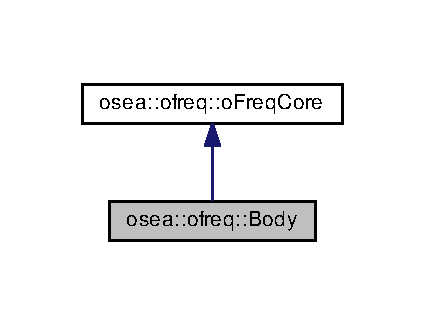
\includegraphics[width=218pt]{classosea_1_1ofreq_1_1_body__inherit__graph}
\end{center}
\end{figure}
\subsection*{Public Member Functions}
\begin{DoxyCompactItemize}
\item 
\hyperlink{classosea_1_1ofreq_1_1_body_a7727b0d8c998bbc2942e4c802e31e2eb}{Body} ()
\item 
\hyperlink{classosea_1_1ofreq_1_1_body_abe1c4da65568cf7978b6247affc461e3}{$\sim$\-Body} ()
\item 
bool \hyperlink{classosea_1_1ofreq_1_1_body_ad4580795d6db4b4ffd23db2a21ace9c7}{operator==} (\hyperlink{classosea_1_1ofreq_1_1_body}{Body} \&bod\-In)
\begin{DoxyCompactList}\small\item\em Overload for operator == to compare two \hyperlink{classosea_1_1ofreq_1_1_body}{Body} objects. Comparison is based on body names. \end{DoxyCompactList}\item 
void \hyperlink{classosea_1_1ofreq_1_1_body_a617bde11c3c42cc2ecbf3d5a7319a904}{set\-Body\-Name} (std\-::string)
\item 
std\-::string \& \hyperlink{classosea_1_1ofreq_1_1_body_ae1f5ffd42ba3b276a056eb56ec6ed5a9}{ref\-Body\-Name} ()
\begin{DoxyCompactList}\small\item\em Exposes the body name property for operation. \end{DoxyCompactList}\item 
std\-::string \& \hyperlink{classosea_1_1ofreq_1_1_body_aef09a9c9b037e1b4e42fbdd1fa61c65d}{ref\-Hydro\-Bod\-Name} ()
\begin{DoxyCompactList}\small\item\em Exposes the hydro body name property for operation. \end{DoxyCompactList}\item 
void \hyperlink{classosea_1_1ofreq_1_1_body_a9fadda19cdff7c41800b5fe3b994b49e}{set\-Hydro\-Bod\-Name} (std\-::string)
\item 
std\-::string \hyperlink{classosea_1_1ofreq_1_1_body_ada5245142768e7b4cdc74504651438bb}{get\-Hydro\-Bod\-Name} ()
\item 
void \hyperlink{classosea_1_1ofreq_1_1_body_a7bba55a8fd4aea7a17ce7bd5f54d6ab8}{set\-Heading} (double)
\item 
double \hyperlink{classosea_1_1ofreq_1_1_body_ac34e65deb4894bd5c2b5d4089be0dcb0}{get\-Heading} ()
\begin{DoxyCompactList}\small\item\em Gets the heading for the body. Heading is measured in radians. Zero heading is True North, proceeding counter clockwise around the compass rose. \end{DoxyCompactList}\item 
double \& \hyperlink{classosea_1_1ofreq_1_1_body_a7aef7cce12d2dbdd3e5ab789ba8fe669}{ref\-Heading} ()
\begin{DoxyCompactList}\small\item\em Exposes the heading property for operations. \end{DoxyCompactList}\item 
void \hyperlink{classosea_1_1ofreq_1_1_body_a896b660a9d001422f5d2b0b4e6d77b98}{set\-Mass} (double)
\item 
double \hyperlink{classosea_1_1ofreq_1_1_body_ac58abb2931cc56f2c0ff85700175a4d9}{get\-Mass} ()
\begin{DoxyCompactList}\small\item\em Returns the mass of the body. \end{DoxyCompactList}\item 
void \hyperlink{classosea_1_1ofreq_1_1_body_a2c9b1a384512fdd3fc5bb017289d1478}{set\-Mom\-Ixx} (double)
\item 
double \hyperlink{classosea_1_1ofreq_1_1_body_ac95aca5c89a30c42db96a8cfacecd89d}{get\-Mom\-Ixx} ()
\begin{DoxyCompactList}\small\item\em Returns the mass moment of inertia on the X\-X axis for the body. \end{DoxyCompactList}\item 
void \hyperlink{classosea_1_1ofreq_1_1_body_a4a92bccc2f40ba7d5fe754428d41195f}{set\-Mom\-Iyy} (double)
\item 
double \hyperlink{classosea_1_1ofreq_1_1_body_ade00f804ca3c40245527f5554580f331}{get\-Mom\-Iyy} ()
\begin{DoxyCompactList}\small\item\em Returns the mass moment of inertia on the Y\-Y axis for the body. \end{DoxyCompactList}\item 
void \hyperlink{classosea_1_1ofreq_1_1_body_a99662066111dcde2dd6fdbf8dd2230dd}{set\-Mom\-Izz} (double)
\item 
double \hyperlink{classosea_1_1ofreq_1_1_body_a00f9b6c0dfc59de42bb4ba6eaa80d707}{get\-Mom\-Izz} ()
\begin{DoxyCompactList}\small\item\em Returns the mass moment of inertia on the Z\-Z axis for the body. \end{DoxyCompactList}\item 
void \hyperlink{classosea_1_1ofreq_1_1_body_ad21041419756e97484ef399181e4b668}{set\-Mom\-Ixy} (double)
\item 
double \hyperlink{classosea_1_1ofreq_1_1_body_a1acaae4a9731de146aabcb9482ff3f0b}{get\-Mom\-Ixy} ()
\begin{DoxyCompactList}\small\item\em Returns the cross product of intertia on the X\-Y axis for the body. \end{DoxyCompactList}\item 
void \hyperlink{classosea_1_1ofreq_1_1_body_ab76083304777794dd27769e1a35955b5}{set\-Mom\-Ixz} (double)
\item 
double \hyperlink{classosea_1_1ofreq_1_1_body_a946ad48ed4493008f4afbc5e89690bb5}{get\-Mom\-Ixz} ()
\begin{DoxyCompactList}\small\item\em Returns the cross product of intertia on the X\-Z axis for the body. \end{DoxyCompactList}\item 
void \hyperlink{classosea_1_1ofreq_1_1_body_a21a26c218ddbb7ee5b20e9ccdb0736f7}{set\-Mom\-Iyz} (double)
\item 
double \hyperlink{classosea_1_1ofreq_1_1_body_a5178058d29b5eaac87f21f26d5e935f6}{get\-Mom\-Iyz} ()
\begin{DoxyCompactList}\small\item\em Returns the cross product of intertia on the Y\-Z axis for the body. \end{DoxyCompactList}\item 
void \hyperlink{classosea_1_1ofreq_1_1_body_aeaacc5db3052196de8a6f7f61a8b6278}{set\-Cen\-X} (double)
\item 
arma\-::\-Mat$<$ double $>$ \hyperlink{classosea_1_1ofreq_1_1_body_a4201150aa57d9d6f3aa245d8eca231d3}{get\-Mass\-Matrix} ()
\begin{DoxyCompactList}\small\item\em Gets the mass matrix for the body. \end{DoxyCompactList}\item 
arma\-::\-Mat$<$ double $>$ \& \hyperlink{classosea_1_1ofreq_1_1_body_acb2895e81a595c7d168db48ff5dc766c}{Mass\-Matrix} ()
\begin{DoxyCompactList}\small\item\em Implements the method \hyperlink{classosea_1_1ofreq_1_1_body_a4201150aa57d9d6f3aa245d8eca231d3}{get\-Mass\-Matrix()}, just under a different name. \end{DoxyCompactList}\item 
void \hyperlink{classosea_1_1ofreq_1_1_body_a8c0801af29b02fa9890ad078368844e8}{set\-Mass\-Matrix} (arma\-::\-Mat$<$ double $>$ Mass\-Mat\-In)
\begin{DoxyCompactList}\small\item\em Set the mass matrix for the body. \end{DoxyCompactList}\item 
double \hyperlink{classosea_1_1ofreq_1_1_body_a7723a89d7d4b893a82dd693571a9449a}{get\-Cen\-X} ()
\begin{DoxyCompactList}\small\item\em Returns the centroid of the body mass, X-\/axis. \end{DoxyCompactList}\item 
void \hyperlink{classosea_1_1ofreq_1_1_body_abebc4472a354ea0d6307ccaff75714db}{set\-Cen\-Y} (double)
\item 
double \hyperlink{classosea_1_1ofreq_1_1_body_a5bafecfaa43dd1cf5deef6ada9d03858}{get\-Cen\-Y} ()
\begin{DoxyCompactList}\small\item\em Returns the centroid of the body mass, Y-\/axis. \end{DoxyCompactList}\item 
void \hyperlink{classosea_1_1ofreq_1_1_body_a866a9f5959854435e8efb688a3d09af7}{set\-Cen\-Z} (double)
\item 
double \hyperlink{classosea_1_1ofreq_1_1_body_aeab53e414035366be2094485ef72c3b7}{get\-Cen\-Z} ()
\begin{DoxyCompactList}\small\item\em Returns the centroid of the body mass, Z-\/axis. \end{DoxyCompactList}\item 
arma\-::\-Mat$<$ double $>$ \hyperlink{classosea_1_1ofreq_1_1_body_a4e48c171b46972f1348fdf140876210e}{get\-Cen} ()
\begin{DoxyCompactList}\small\item\em Returns the entire mass centroid matrix. \end{DoxyCompactList}\item 
void \hyperlink{classosea_1_1ofreq_1_1_body_af507be7e52f44404e7664dd623585780}{set\-Posn\-X} (double input)
\begin{DoxyCompactList}\small\item\em Sets the body position in the X-\/axis. \end{DoxyCompactList}\item 
double \hyperlink{classosea_1_1ofreq_1_1_body_ad649f4405ae4b8e91f69e5e54ff68dcd}{get\-Posn\-X} ()
\begin{DoxyCompactList}\small\item\em Gets the body position in the X-\/axis. \end{DoxyCompactList}\item 
void \hyperlink{classosea_1_1ofreq_1_1_body_a782d1cf6280cebe6857a1aef764d2572}{set\-Posn\-Y} (double input)
\begin{DoxyCompactList}\small\item\em Sets the body position in the Y-\/axis. \end{DoxyCompactList}\item 
double \hyperlink{classosea_1_1ofreq_1_1_body_ad4b9a74035b9fcb1af31d2ce300911c4}{get\-Posn\-Y} ()
\begin{DoxyCompactList}\small\item\em Gets the body position in the Y-\/axis. \end{DoxyCompactList}\item 
void \hyperlink{classosea_1_1ofreq_1_1_body_a36a7e543c0bdad30bb16eda563543ac4}{set\-Posn\-Z} (double input)
\begin{DoxyCompactList}\small\item\em Sets the body position in the Z-\/axis. \end{DoxyCompactList}\item 
double \hyperlink{classosea_1_1ofreq_1_1_body_aaeddfd614683a8bc7fe81383667314a9}{get\-Posn\-Z} ()
\begin{DoxyCompactList}\small\item\em Gets the body position in the Z-\/axis. \end{DoxyCompactList}\item 
arma\-::\-Mat$<$ double $>$ \hyperlink{classosea_1_1ofreq_1_1_body_a09987e449c77ba11fb66cf81de88220a}{get\-Posn} ()
\begin{DoxyCompactList}\small\item\em Returns the entire matrix for position of the body. \end{DoxyCompactList}\item 
arma\-::\-Mat$<$ double $>$ \& \hyperlink{classosea_1_1ofreq_1_1_body_ad34f38992e14d5bda02c481c311b66b3}{ref\-Posn} ()
\begin{DoxyCompactList}\small\item\em Exposes the position property for operation. The entire matrix for position of the body. \end{DoxyCompactList}\item 
std\-::string \hyperlink{classosea_1_1ofreq_1_1_body_aab63febbe35984d8551a188b40ee3c3f}{get\-Body\-Name} ()
\item 
void \hyperlink{classosea_1_1ofreq_1_1_body_a4131658e5b392e8a5cd6475b69fae06d}{set\-Soln\-Mat} (arma\-::cx\-\_\-mat input)
\begin{DoxyCompactList}\small\item\em Set the solution matrix for the body. \end{DoxyCompactList}\item 
arma\-::cx\-\_\-mat \hyperlink{classosea_1_1ofreq_1_1_body_a5153b4cfad5bf12ae6f279a5e7190c31}{get\-Solution} ()
\begin{DoxyCompactList}\small\item\em Get the solution matrix for the body. \end{DoxyCompactList}\item 
arma\-::cx\-\_\-mat \& \hyperlink{classosea_1_1ofreq_1_1_body_ae799af5531c35381830061f6abc0bb17}{ref\-Solution} ()
\begin{DoxyCompactList}\small\item\em Get the solution matrix for the body. \end{DoxyCompactList}\item 
arma\-::cx\-\_\-mat \& \hyperlink{classosea_1_1ofreq_1_1_body_af22d8750d2ce8a85c4896a0261569f63}{ref\-Data\-Solution} ()
\begin{DoxyCompactList}\small\item\em The same things as the \hyperlink{classosea_1_1ofreq_1_1_body_ae799af5531c35381830061f6abc0bb17}{ref\-Solution()} function, just under a different name. \end{DoxyCompactList}\item 
\hyperlink{namespaceosea_1_1ofreq_a40cad4695a41123a7ae6ab0b6e8b1664}{complex\-Double} \& \hyperlink{classosea_1_1ofreq_1_1_body_a5459de639385a8a5dd32a5591aabeee9}{ref\-Data\-Solution} (int var\-Index\-In)
\begin{DoxyCompactList}\small\item\em Returns a single solution value, based on the variable requested. \end{DoxyCompactList}\item 
\hyperlink{classosea_1_1ofreq_1_1_body}{Body} \hyperlink{classosea_1_1ofreq_1_1_body_a370dc9a5702d93d9295a9618ebdef456}{Copy} ()
\begin{DoxyCompactList}\small\item\em Copies the body object, complete with all current data. \end{DoxyCompactList}\item 
std\-::vector$<$ \hyperlink{classosea_1_1ofreq_1_1_force_active}{Force\-Active} $\ast$ $>$ \& \hyperlink{classosea_1_1ofreq_1_1_body_ab9373ca18d09e89a2ba535c66fa92760}{list\-Force\-Active\-\_\-user} ()
\begin{DoxyCompactList}\small\item\em The list of active user forces. \end{DoxyCompactList}\item 
\hyperlink{classosea_1_1ofreq_1_1_force_active}{Force\-Active} $\ast$ \hyperlink{classosea_1_1ofreq_1_1_body_ad55994a87e95520959a2d236e02168ea}{list\-Force\-Active\-\_\-user} (int force\-In)
\begin{DoxyCompactList}\small\item\em A single active user force. \end{DoxyCompactList}\item 
std\-::vector$<$ \hyperlink{classosea_1_1ofreq_1_1_force_active}{Force\-Active} $\ast$ $>$ \& \hyperlink{classosea_1_1ofreq_1_1_body_a2169495533eebe0f4f05d9e2cb71f42b}{list\-Force\-Active\-\_\-hydro} ()
\begin{DoxyCompactList}\small\item\em The list of active hydrodynamic forces. \end{DoxyCompactList}\item 
\hyperlink{classosea_1_1ofreq_1_1_force_active}{Force\-Active} $\ast$ \hyperlink{classosea_1_1ofreq_1_1_body_aa83129940f0eb3a27686b35292bf3339}{list\-Force\-Active\-\_\-hydro} (int force\-In)
\begin{DoxyCompactList}\small\item\em A single active hydrodynamic force. \end{DoxyCompactList}\item 
std\-::vector$<$ \hyperlink{classosea_1_1ofreq_1_1_force_react}{Force\-React} $\ast$ $>$ \& \hyperlink{classosea_1_1ofreq_1_1_body_afc1e6e0018dd26cc3702b74aea12ed9b}{list\-Force\-React\-\_\-user} ()
\begin{DoxyCompactList}\small\item\em The list of reactive user forces. \end{DoxyCompactList}\item 
\hyperlink{classosea_1_1ofreq_1_1_force_react}{Force\-React} $\ast$ \hyperlink{classosea_1_1ofreq_1_1_body_a8afe32e16a7869395083de6cb0aca63e}{list\-Force\-React\-\_\-user} (int force\-In)
\begin{DoxyCompactList}\small\item\em A single reactive user force. \end{DoxyCompactList}\item 
std\-::vector$<$ \hyperlink{classosea_1_1ofreq_1_1_force_react}{Force\-React} $\ast$ $>$ \& \hyperlink{classosea_1_1ofreq_1_1_body_ad68893d21ecf337242d68936132ad25a}{list\-Force\-React\-\_\-hydro} ()
\begin{DoxyCompactList}\small\item\em The list of reactive hydrodynamic forces. \end{DoxyCompactList}\item 
\hyperlink{classosea_1_1ofreq_1_1_force_react}{Force\-React} $\ast$ \hyperlink{classosea_1_1ofreq_1_1_body_a774fe4681465ee5a8ea344f4ec7c18e2}{list\-Force\-React\-\_\-hydro} (int force\-In)
\begin{DoxyCompactList}\small\item\em A single reactive hydrodynamic force. \end{DoxyCompactList}\item 
std\-::vector$<$ \hyperlink{classosea_1_1ofreq_1_1_force_cross}{Force\-Cross} $\ast$ $>$ \& \hyperlink{classosea_1_1ofreq_1_1_body_ac428c19730346a51bde800e0cbc2e281}{list\-Force\-Cross\-\_\-user} ()
\begin{DoxyCompactList}\small\item\em The list of user cross-\/body forces. \end{DoxyCompactList}\item 
\hyperlink{classosea_1_1ofreq_1_1_force_cross}{Force\-Cross} $\ast$ \hyperlink{classosea_1_1ofreq_1_1_body_af01cd5dc37ebd7969f4f2bc10ba3d76b}{list\-Force\-Cross\-\_\-user} (int force\-In)
\begin{DoxyCompactList}\small\item\em A single cross-\/body user force. \end{DoxyCompactList}\item 
std\-::vector$<$ \hyperlink{classosea_1_1ofreq_1_1_force_cross}{Force\-Cross} $\ast$ $>$ \& \hyperlink{classosea_1_1ofreq_1_1_body_a0dc70d3a67ad921a022f48a2fdf37526}{list\-Force\-Cross\-\_\-hydro} ()
\begin{DoxyCompactList}\small\item\em The list of hydrodynamic cross-\/body forces. \end{DoxyCompactList}\item 
\hyperlink{classosea_1_1ofreq_1_1_force_cross}{Force\-Cross} $\ast$ \hyperlink{classosea_1_1ofreq_1_1_body_ab814600b31abd49c0a8de29a0fb597b4}{list\-Force\-Cross\-\_\-hydro} (int force\-In)
\begin{DoxyCompactList}\small\item\em A single cross-\/body hydrodynamic force. \end{DoxyCompactList}\item 
std\-::vector$<$ \hyperlink{classosea_1_1ofreq_1_1_body}{Body} $\ast$ $>$ \& \hyperlink{classosea_1_1ofreq_1_1_body_a56ad2b60555f24df3feb5889974b27b2}{list\-Cross\-Body\-\_\-user} ()
\begin{DoxyCompactList}\small\item\em The list of linked bodies for user cross-\/body forces. \end{DoxyCompactList}\item 
\hyperlink{classosea_1_1ofreq_1_1_body}{Body} \& \hyperlink{classosea_1_1ofreq_1_1_body_afaf64ab1b477ff157f31e6824be1b767}{list\-Cross\-Body\-\_\-user} (int index)
\begin{DoxyCompactList}\small\item\em Returns reference to individual linked \hyperlink{classosea_1_1ofreq_1_1_body}{Body} for the user cross-\/body force. \end{DoxyCompactList}\item 
std\-::vector$<$ \hyperlink{classosea_1_1ofreq_1_1_body}{Body} $\ast$ $>$ \& \hyperlink{classosea_1_1ofreq_1_1_body_a7c930213d83962d4248068c38c589113}{list\-Cross\-Body\-\_\-hydro} ()
\begin{DoxyCompactList}\small\item\em The list of linked bodies for hydrodynamic cross-\/body forces. \end{DoxyCompactList}\item 
\hyperlink{classosea_1_1ofreq_1_1_body}{Body} \& \hyperlink{classosea_1_1ofreq_1_1_body_a9aaac9391781c67198f7b8b5785d4745}{list\-Cross\-Body\-\_\-hydro} (int index)
\begin{DoxyCompactList}\small\item\em Returns reference to individual linked \hyperlink{classosea_1_1ofreq_1_1_body}{Body} for the hydro cross-\/body force. \end{DoxyCompactList}\item 
std\-::vector$<$ std\-::string $>$ \& \hyperlink{classosea_1_1ofreq_1_1_body_a07d8ed6fdf5a4c6ef73b2d39b58403ce}{list\-Named\-Link\-\_\-user} ()
\begin{DoxyCompactList}\small\item\em The list of names of linked bodies for user cross-\/body forces. This is a list of names of other bodies that a cross-\/body force references. This corresponds to the vector list\-Force\-Cross\-\_\-usr. The indices of the two vectors should match. So that when a force gets added at index 5 in the list\-Force\-Cross\-\_\-user, it should have a matching entry at index 5 in list\-Named\-Link\-\_\-usr. The list of names only is a temporary list used during the input stage of bodies. This is required because the linked body may name a body which is not yet read from the input file. Thus, the body is not currently defined. Once all Bodies are defined, the \hyperlink{classosea_1_1ofreq_1_1_system}{System} object calls a function to read through each name in the list and assign corresponding pointers in the list\-Linked\-Body\-\_\-usr. \end{DoxyCompactList}\item 
std\-::string \& \hyperlink{classosea_1_1ofreq_1_1_body_a1fd7e672b9768351f9a53523d7b5c798}{list\-Named\-Link\-\_\-user} (unsigned int var\-In)
\begin{DoxyCompactList}\small\item\em The list of names of linked bodies for user cross-\/body forces. This is a list of names of other bodies that a cross-\/body force references. This corresponds to the vector list\-Force\-Cross\-\_\-usr. The indices of the two vectors should match. So that when a force gets added at index 5 in the list\-Force\-Cross\-\_\-user, it should have a matching entry at index 5 in list\-Named\-Link\-\_\-usr. The list of names only is a temporary list used during the input stage of bodies. This is required because the linked body may name a body which is not yet read from the input file. Thus, the body is not currently defined. Once all Bodies are defined, the \hyperlink{classosea_1_1ofreq_1_1_system}{System} object calls a function to read through each name in the list and assign corresponding pointers in the list\-Linked\-Body\-\_\-usr. \end{DoxyCompactList}\item 
std\-::vector$<$ std\-::string $>$ \& \hyperlink{classosea_1_1ofreq_1_1_body_abc4abd052a3776123df114c6faf34bae}{list\-Named\-Link\-\_\-hydro} ()
\begin{DoxyCompactList}\small\item\em The list of names of linked bodies for hydro cross-\/body forces. This is a list of names of other bodies that a cross-\/body force references. This corresponds to the vector list\-Force\-Cross\-\_\-hydro. The indices of the two vectors should match. So that when a force gets added at index 5 in the list\-Force\-Cross\-\_\-hydro, it should have a matching entry at index 5 in list\-Named\-Link\-\_\-hydro. The list of names only is a temporary list used during the input stage of bodies. This is required because the linked body may name a body which is not yet read from the input file. Thus, the body is not currently defined. Once all Bodies are defined, the \hyperlink{classosea_1_1ofreq_1_1_system}{System} object calls a function to read through each name in the list and assign corresponding pointers in the list\-Linked\-Body\-\_\-hydro. \end{DoxyCompactList}\item 
std\-::string \& \hyperlink{classosea_1_1ofreq_1_1_body_ad01b96bf575dde9f75f489c7118ca574}{list\-Named\-Link\-\_\-hydro} (unsigned int var\-In)
\begin{DoxyCompactList}\small\item\em The list of names of linked bodies for hydro cross-\/body forces. This is a list of names of other bodies that a cross-\/body force references. This corresponds to the vector list\-Force\-Cross\-\_\-hydro. The indices of the two vectors should match. So that when a force gets added at index 5 in the list\-Force\-Cross\-\_\-hydro, it should have a matching entry at index 5 in list\-Named\-Link\-\_\-hydro. The list of names only is a temporary list used during the input stage of bodies. This is required because the linked body may name a body which is not yet read from the input file. Thus, the body is not currently defined. Once all Bodies are defined, the \hyperlink{classosea_1_1ofreq_1_1_system}{System} object calls a function to read through each name in the list and assign corresponding pointers in the list\-Linked\-Body\-\_\-hydro. \end{DoxyCompactList}\item 
void \hyperlink{classosea_1_1ofreq_1_1_body_a25b6fa24ac6237272494a7f74a348145}{set\-Motion\-Model} (\hyperlink{classosea_1_1ofreq_1_1_motion_model}{ofreq\-::\-Motion\-Model} \&model\-In)
\begin{DoxyCompactList}\small\item\em Sets the motion model for lookup later. \end{DoxyCompactList}\item 
\hyperlink{classosea_1_1ofreq_1_1_motion_model}{ofreq\-::\-Motion\-Model} \& \hyperlink{classosea_1_1ofreq_1_1_body_a00aa77588d908d6df47a923dc8bf8331}{get\-Motion\-Model} ()
\begin{DoxyCompactList}\small\item\em Gets the motion model. \end{DoxyCompactList}\item 
int \hyperlink{classosea_1_1ofreq_1_1_body_a07a8f186c02f0d5bad4beded83949571}{get\-Equation\-Count} ()
\begin{DoxyCompactList}\small\item\em Gets the number of equations used in the body. \end{DoxyCompactList}\item 
void \hyperlink{classosea_1_1ofreq_1_1_body_a1d5dfa0c6db92dd1d4cf3cd7bafbef34}{init\-Mass\-Mat} ()
\begin{DoxyCompactList}\small\item\em Initializes the mass matrix. Resizes it to the correct value. Only acts if the motion model is already set. And does not override any current values of the mass matrix. \end{DoxyCompactList}\end{DoxyCompactItemize}
\subsection*{Additional Inherited Members}


\subsection{Detailed Description}
This class holds all of the data for the \hyperlink{classosea_1_1ofreq_1_1_body}{Body} Input File. 

Definition at line 103 of file body.\-h.



\subsection{Constructor \& Destructor Documentation}
\hypertarget{classosea_1_1ofreq_1_1_body_a7727b0d8c998bbc2942e4c802e31e2eb}{\index{osea\-::ofreq\-::\-Body@{osea\-::ofreq\-::\-Body}!Body@{Body}}
\index{Body@{Body}!osea::ofreq::Body@{osea\-::ofreq\-::\-Body}}
\subsubsection[{Body}]{\setlength{\rightskip}{0pt plus 5cm}Body\-::\-Body (
\begin{DoxyParamCaption}
{}
\end{DoxyParamCaption}
)}}\label{classosea_1_1ofreq_1_1_body_a7727b0d8c998bbc2942e4c802e31e2eb}
The default constructor 

Definition at line 44 of file body.\-cpp.

\hypertarget{classosea_1_1ofreq_1_1_body_abe1c4da65568cf7978b6247affc461e3}{\index{osea\-::ofreq\-::\-Body@{osea\-::ofreq\-::\-Body}!$\sim$\-Body@{$\sim$\-Body}}
\index{$\sim$\-Body@{$\sim$\-Body}!osea::ofreq::Body@{osea\-::ofreq\-::\-Body}}
\subsubsection[{$\sim$\-Body}]{\setlength{\rightskip}{0pt plus 5cm}Body\-::$\sim$\-Body (
\begin{DoxyParamCaption}
{}
\end{DoxyParamCaption}
)}}\label{classosea_1_1ofreq_1_1_body_abe1c4da65568cf7978b6247affc461e3}
The default destructor, nothing happens here. 

Definition at line 53 of file body.\-cpp.



\subsection{Member Function Documentation}
\hypertarget{classosea_1_1ofreq_1_1_body_a370dc9a5702d93d9295a9618ebdef456}{\index{osea\-::ofreq\-::\-Body@{osea\-::ofreq\-::\-Body}!Copy@{Copy}}
\index{Copy@{Copy}!osea::ofreq::Body@{osea\-::ofreq\-::\-Body}}
\subsubsection[{Copy}]{\setlength{\rightskip}{0pt plus 5cm}{\bf Body} Body\-::\-Copy (
\begin{DoxyParamCaption}
{}
\end{DoxyParamCaption}
)}}\label{classosea_1_1ofreq_1_1_body_a370dc9a5702d93d9295a9618ebdef456}


Copies the body object, complete with all current data. 

\begin{DoxyReturn}{Returns}
Returns a copy of the body object, complete with all current data. Passed by value, not reference. 
\end{DoxyReturn}


Definition at line 730 of file body.\-cpp.

\hypertarget{classosea_1_1ofreq_1_1_body_aab63febbe35984d8551a188b40ee3c3f}{\index{osea\-::ofreq\-::\-Body@{osea\-::ofreq\-::\-Body}!get\-Body\-Name@{get\-Body\-Name}}
\index{get\-Body\-Name@{get\-Body\-Name}!osea::ofreq::Body@{osea\-::ofreq\-::\-Body}}
\subsubsection[{get\-Body\-Name}]{\setlength{\rightskip}{0pt plus 5cm}string Body\-::get\-Body\-Name (
\begin{DoxyParamCaption}
{}
\end{DoxyParamCaption}
)}}\label{classosea_1_1ofreq_1_1_body_aab63febbe35984d8551a188b40ee3c3f}
Get the name of the body. \begin{DoxyReturn}{Returns}
The name of the body. 
\end{DoxyReturn}


Definition at line 690 of file body.\-cpp.

\hypertarget{classosea_1_1ofreq_1_1_body_a4e48c171b46972f1348fdf140876210e}{\index{osea\-::ofreq\-::\-Body@{osea\-::ofreq\-::\-Body}!get\-Cen@{get\-Cen}}
\index{get\-Cen@{get\-Cen}!osea::ofreq::Body@{osea\-::ofreq\-::\-Body}}
\subsubsection[{get\-Cen}]{\setlength{\rightskip}{0pt plus 5cm}Mat$<$ double $>$ Body\-::get\-Cen (
\begin{DoxyParamCaption}
{}
\end{DoxyParamCaption}
)}}\label{classosea_1_1ofreq_1_1_body_a4e48c171b46972f1348fdf140876210e}


Returns the entire mass centroid matrix. 

\begin{DoxyReturn}{Returns}
Returns the entire mass centroid matrix. Output is a 3x1 matrix of the body centroid, relative to body coordinate system. 
\end{DoxyReturn}


Definition at line 623 of file body.\-cpp.

\hypertarget{classosea_1_1ofreq_1_1_body_a7723a89d7d4b893a82dd693571a9449a}{\index{osea\-::ofreq\-::\-Body@{osea\-::ofreq\-::\-Body}!get\-Cen\-X@{get\-Cen\-X}}
\index{get\-Cen\-X@{get\-Cen\-X}!osea::ofreq::Body@{osea\-::ofreq\-::\-Body}}
\subsubsection[{get\-Cen\-X}]{\setlength{\rightskip}{0pt plus 5cm}double Body\-::get\-Cen\-X (
\begin{DoxyParamCaption}
{}
\end{DoxyParamCaption}
)}}\label{classosea_1_1ofreq_1_1_body_a7723a89d7d4b893a82dd693571a9449a}


Returns the centroid of the body mass, X-\/axis. 

Returns the centroid of the body mass, X-\/axis. Centroid is relative to body coordinates. This includes body rotation and translation. \begin{DoxyReturn}{Returns}
Returns the centroid of the body mass, X-\/axis. Centroid is relative to body coordinates. This includes body rotation and translation. 
\end{DoxyReturn}


Definition at line 587 of file body.\-cpp.

\hypertarget{classosea_1_1ofreq_1_1_body_a5bafecfaa43dd1cf5deef6ada9d03858}{\index{osea\-::ofreq\-::\-Body@{osea\-::ofreq\-::\-Body}!get\-Cen\-Y@{get\-Cen\-Y}}
\index{get\-Cen\-Y@{get\-Cen\-Y}!osea::ofreq::Body@{osea\-::ofreq\-::\-Body}}
\subsubsection[{get\-Cen\-Y}]{\setlength{\rightskip}{0pt plus 5cm}double Body\-::get\-Cen\-Y (
\begin{DoxyParamCaption}
{}
\end{DoxyParamCaption}
)}}\label{classosea_1_1ofreq_1_1_body_a5bafecfaa43dd1cf5deef6ada9d03858}


Returns the centroid of the body mass, Y-\/axis. 

Returns the centroid of the body mass, Y-\/axis. Centroid is relative to body coordinates. This includes body rotation and translation. \begin{DoxyReturn}{Returns}
Returns the centroid of the body mass, Y-\/axis. Centroid is relative to body coordinates. This includes body rotation and translation. 
\end{DoxyReturn}


Definition at line 602 of file body.\-cpp.

\hypertarget{classosea_1_1ofreq_1_1_body_aeab53e414035366be2094485ef72c3b7}{\index{osea\-::ofreq\-::\-Body@{osea\-::ofreq\-::\-Body}!get\-Cen\-Z@{get\-Cen\-Z}}
\index{get\-Cen\-Z@{get\-Cen\-Z}!osea::ofreq::Body@{osea\-::ofreq\-::\-Body}}
\subsubsection[{get\-Cen\-Z}]{\setlength{\rightskip}{0pt plus 5cm}double Body\-::get\-Cen\-Z (
\begin{DoxyParamCaption}
{}
\end{DoxyParamCaption}
)}}\label{classosea_1_1ofreq_1_1_body_aeab53e414035366be2094485ef72c3b7}


Returns the centroid of the body mass, Z-\/axis. 

Returns the centroid of the body mass, Z-\/axis. Centroid is relative to body coordinates. This includes body rotation and translation. \begin{DoxyReturn}{Returns}
Returns the centroid of the body mass, Z-\/axis. Centroid is relative to body coordinates. This includes body rotation and translation. 
\end{DoxyReturn}


Definition at line 617 of file body.\-cpp.

\hypertarget{classosea_1_1ofreq_1_1_body_a07a8f186c02f0d5bad4beded83949571}{\index{osea\-::ofreq\-::\-Body@{osea\-::ofreq\-::\-Body}!get\-Equation\-Count@{get\-Equation\-Count}}
\index{get\-Equation\-Count@{get\-Equation\-Count}!osea::ofreq::Body@{osea\-::ofreq\-::\-Body}}
\subsubsection[{get\-Equation\-Count}]{\setlength{\rightskip}{0pt plus 5cm}int Body\-::get\-Equation\-Count (
\begin{DoxyParamCaption}
{}
\end{DoxyParamCaption}
)}}\label{classosea_1_1ofreq_1_1_body_a07a8f186c02f0d5bad4beded83949571}


Gets the number of equations used in the body. 

Gets the number of equations used in the body. \begin{DoxyReturn}{Returns}
Integer number representing the number of equations used in the body. 
\end{DoxyReturn}


Definition at line 999 of file body.\-cpp.



Here is the call graph for this function\-:\nopagebreak
\begin{figure}[H]
\begin{center}
\leavevmode
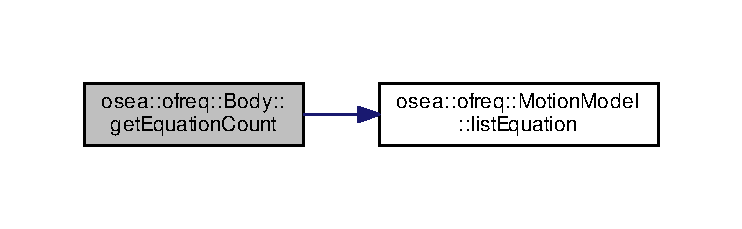
\includegraphics[width=350pt]{classosea_1_1ofreq_1_1_body_a07a8f186c02f0d5bad4beded83949571_cgraph}
\end{center}
\end{figure}


\hypertarget{classosea_1_1ofreq_1_1_body_ac34e65deb4894bd5c2b5d4089be0dcb0}{\index{osea\-::ofreq\-::\-Body@{osea\-::ofreq\-::\-Body}!get\-Heading@{get\-Heading}}
\index{get\-Heading@{get\-Heading}!osea::ofreq::Body@{osea\-::ofreq\-::\-Body}}
\subsubsection[{get\-Heading}]{\setlength{\rightskip}{0pt plus 5cm}double Body\-::get\-Heading (
\begin{DoxyParamCaption}
{}
\end{DoxyParamCaption}
)}}\label{classosea_1_1ofreq_1_1_body_ac34e65deb4894bd5c2b5d4089be0dcb0}


Gets the heading for the body. Heading is measured in radians. Zero heading is True North, proceeding counter clockwise around the compass rose. 

\begin{DoxyReturn}{Returns}
Returns double variable. Heading of the \hyperlink{classosea_1_1ofreq_1_1_body}{Body} object. Variable passed by value. 
\end{DoxyReturn}


Definition at line 193 of file body.\-cpp.

\hypertarget{classosea_1_1ofreq_1_1_body_ada5245142768e7b4cdc74504651438bb}{\index{osea\-::ofreq\-::\-Body@{osea\-::ofreq\-::\-Body}!get\-Hydro\-Bod\-Name@{get\-Hydro\-Bod\-Name}}
\index{get\-Hydro\-Bod\-Name@{get\-Hydro\-Bod\-Name}!osea::ofreq::Body@{osea\-::ofreq\-::\-Body}}
\subsubsection[{get\-Hydro\-Bod\-Name}]{\setlength{\rightskip}{0pt plus 5cm}string Body\-::get\-Hydro\-Bod\-Name (
\begin{DoxyParamCaption}
{}
\end{DoxyParamCaption}
)}}\label{classosea_1_1ofreq_1_1_body_ada5245142768e7b4cdc74504651438bb}
Gets the name of the hydro body. \begin{DoxyReturn}{Returns}
Returns std\-::string. The name of the hydrobody object associated with the body. Variable passed by value. 
\end{DoxyReturn}


Definition at line 181 of file body.\-cpp.

\hypertarget{classosea_1_1ofreq_1_1_body_ac58abb2931cc56f2c0ff85700175a4d9}{\index{osea\-::ofreq\-::\-Body@{osea\-::ofreq\-::\-Body}!get\-Mass@{get\-Mass}}
\index{get\-Mass@{get\-Mass}!osea::ofreq::Body@{osea\-::ofreq\-::\-Body}}
\subsubsection[{get\-Mass}]{\setlength{\rightskip}{0pt plus 5cm}double Body\-::get\-Mass (
\begin{DoxyParamCaption}
{}
\end{DoxyParamCaption}
)}}\label{classosea_1_1ofreq_1_1_body_ac58abb2931cc56f2c0ff85700175a4d9}


Returns the mass of the body. 

\begin{DoxyReturn}{Returns}
Returns the mass of the body. Output is in units of kilograms. 
\end{DoxyReturn}


Definition at line 253 of file body.\-cpp.

\hypertarget{classosea_1_1ofreq_1_1_body_a4201150aa57d9d6f3aa245d8eca231d3}{\index{osea\-::ofreq\-::\-Body@{osea\-::ofreq\-::\-Body}!get\-Mass\-Matrix@{get\-Mass\-Matrix}}
\index{get\-Mass\-Matrix@{get\-Mass\-Matrix}!osea::ofreq::Body@{osea\-::ofreq\-::\-Body}}
\subsubsection[{get\-Mass\-Matrix}]{\setlength{\rightskip}{0pt plus 5cm}Mat$<$ double $>$ Body\-::get\-Mass\-Matrix (
\begin{DoxyParamCaption}
{}
\end{DoxyParamCaption}
)}}\label{classosea_1_1ofreq_1_1_body_a4201150aa57d9d6f3aa245d8eca231d3}


Gets the mass matrix for the body. 

\begin{DoxyReturn}{Returns}
Returns the mass matrix for the body, as a single matrix. Returned by value. 
\end{DoxyReturn}


Definition at line 548 of file body.\-cpp.

\hypertarget{classosea_1_1ofreq_1_1_body_ac95aca5c89a30c42db96a8cfacecd89d}{\index{osea\-::ofreq\-::\-Body@{osea\-::ofreq\-::\-Body}!get\-Mom\-Ixx@{get\-Mom\-Ixx}}
\index{get\-Mom\-Ixx@{get\-Mom\-Ixx}!osea::ofreq::Body@{osea\-::ofreq\-::\-Body}}
\subsubsection[{get\-Mom\-Ixx}]{\setlength{\rightskip}{0pt plus 5cm}double Body\-::get\-Mom\-Ixx (
\begin{DoxyParamCaption}
{}
\end{DoxyParamCaption}
)}}\label{classosea_1_1ofreq_1_1_body_ac95aca5c89a30c42db96a8cfacecd89d}


Returns the mass moment of inertia on the X\-X axis for the body. 

\begin{DoxyReturn}{Returns}
Returns the mass moment of inertia on the X\-X axis for the body. Output is in units of kilogram-\/m$^\wedge$2. 
\end{DoxyReturn}


Definition at line 311 of file body.\-cpp.

\hypertarget{classosea_1_1ofreq_1_1_body_a1acaae4a9731de146aabcb9482ff3f0b}{\index{osea\-::ofreq\-::\-Body@{osea\-::ofreq\-::\-Body}!get\-Mom\-Ixy@{get\-Mom\-Ixy}}
\index{get\-Mom\-Ixy@{get\-Mom\-Ixy}!osea::ofreq::Body@{osea\-::ofreq\-::\-Body}}
\subsubsection[{get\-Mom\-Ixy}]{\setlength{\rightskip}{0pt plus 5cm}double Body\-::get\-Mom\-Ixy (
\begin{DoxyParamCaption}
{}
\end{DoxyParamCaption}
)}}\label{classosea_1_1ofreq_1_1_body_a1acaae4a9731de146aabcb9482ff3f0b}


Returns the cross product of intertia on the X\-Y axis for the body. 

\begin{DoxyReturn}{Returns}
Returns the cross product of intertia on the X\-Y axis for the body. O\-Utput is in units of kilogram-\/m$^\wedge$2. 
\end{DoxyReturn}


Definition at line 438 of file body.\-cpp.

\hypertarget{classosea_1_1ofreq_1_1_body_a946ad48ed4493008f4afbc5e89690bb5}{\index{osea\-::ofreq\-::\-Body@{osea\-::ofreq\-::\-Body}!get\-Mom\-Ixz@{get\-Mom\-Ixz}}
\index{get\-Mom\-Ixz@{get\-Mom\-Ixz}!osea::ofreq::Body@{osea\-::ofreq\-::\-Body}}
\subsubsection[{get\-Mom\-Ixz}]{\setlength{\rightskip}{0pt plus 5cm}double Body\-::get\-Mom\-Ixz (
\begin{DoxyParamCaption}
{}
\end{DoxyParamCaption}
)}}\label{classosea_1_1ofreq_1_1_body_a946ad48ed4493008f4afbc5e89690bb5}


Returns the cross product of intertia on the X\-Z axis for the body. 

\begin{DoxyReturn}{Returns}
Returns the cross product of intertia on the X\-Z axis for the body. O\-Utput is in units of kilogram-\/m$^\wedge$2. 
\end{DoxyReturn}


Definition at line 482 of file body.\-cpp.

\hypertarget{classosea_1_1ofreq_1_1_body_ade00f804ca3c40245527f5554580f331}{\index{osea\-::ofreq\-::\-Body@{osea\-::ofreq\-::\-Body}!get\-Mom\-Iyy@{get\-Mom\-Iyy}}
\index{get\-Mom\-Iyy@{get\-Mom\-Iyy}!osea::ofreq::Body@{osea\-::ofreq\-::\-Body}}
\subsubsection[{get\-Mom\-Iyy}]{\setlength{\rightskip}{0pt plus 5cm}double Body\-::get\-Mom\-Iyy (
\begin{DoxyParamCaption}
{}
\end{DoxyParamCaption}
)}}\label{classosea_1_1ofreq_1_1_body_ade00f804ca3c40245527f5554580f331}


Returns the mass moment of inertia on the Y\-Y axis for the body. 

\begin{DoxyReturn}{Returns}
Returns the mass moment of inertia on the Y\-Y axis for the body. Output is in units of kilogram-\/m$^\wedge$2. 
\end{DoxyReturn}


Definition at line 353 of file body.\-cpp.

\hypertarget{classosea_1_1ofreq_1_1_body_a5178058d29b5eaac87f21f26d5e935f6}{\index{osea\-::ofreq\-::\-Body@{osea\-::ofreq\-::\-Body}!get\-Mom\-Iyz@{get\-Mom\-Iyz}}
\index{get\-Mom\-Iyz@{get\-Mom\-Iyz}!osea::ofreq::Body@{osea\-::ofreq\-::\-Body}}
\subsubsection[{get\-Mom\-Iyz}]{\setlength{\rightskip}{0pt plus 5cm}double Body\-::get\-Mom\-Iyz (
\begin{DoxyParamCaption}
{}
\end{DoxyParamCaption}
)}}\label{classosea_1_1ofreq_1_1_body_a5178058d29b5eaac87f21f26d5e935f6}


Returns the cross product of intertia on the Y\-Z axis for the body. 

\begin{DoxyReturn}{Returns}
Returns the cross product of intertia on the Y\-Z axis for the body. O\-Utput is in units of kilogram-\/m$^\wedge$2. 
\end{DoxyReturn}


Definition at line 526 of file body.\-cpp.

\hypertarget{classosea_1_1ofreq_1_1_body_a00f9b6c0dfc59de42bb4ba6eaa80d707}{\index{osea\-::ofreq\-::\-Body@{osea\-::ofreq\-::\-Body}!get\-Mom\-Izz@{get\-Mom\-Izz}}
\index{get\-Mom\-Izz@{get\-Mom\-Izz}!osea::ofreq::Body@{osea\-::ofreq\-::\-Body}}
\subsubsection[{get\-Mom\-Izz}]{\setlength{\rightskip}{0pt plus 5cm}double Body\-::get\-Mom\-Izz (
\begin{DoxyParamCaption}
{}
\end{DoxyParamCaption}
)}}\label{classosea_1_1ofreq_1_1_body_a00f9b6c0dfc59de42bb4ba6eaa80d707}


Returns the mass moment of inertia on the Z\-Z axis for the body. 

\begin{DoxyReturn}{Returns}
Returns the mass moment of inertia on the Z\-Z axis for the body. Output is in units of kilogram-\/m$^\wedge$2. 
\end{DoxyReturn}


Definition at line 395 of file body.\-cpp.

\hypertarget{classosea_1_1ofreq_1_1_body_a00aa77588d908d6df47a923dc8bf8331}{\index{osea\-::ofreq\-::\-Body@{osea\-::ofreq\-::\-Body}!get\-Motion\-Model@{get\-Motion\-Model}}
\index{get\-Motion\-Model@{get\-Motion\-Model}!osea::ofreq::Body@{osea\-::ofreq\-::\-Body}}
\subsubsection[{get\-Motion\-Model}]{\setlength{\rightskip}{0pt plus 5cm}{\bf Motion\-Model} \& Body\-::get\-Motion\-Model (
\begin{DoxyParamCaption}
{}
\end{DoxyParamCaption}
)}}\label{classosea_1_1ofreq_1_1_body_a00aa77588d908d6df47a923dc8bf8331}


Gets the motion model. 

Returns the motion model object used by this body object. \begin{DoxyReturn}{Returns}
Returns Motin\-Model object. Variable passed by reference. 
\end{DoxyReturn}


Definition at line 993 of file body.\-cpp.

\hypertarget{classosea_1_1ofreq_1_1_body_a09987e449c77ba11fb66cf81de88220a}{\index{osea\-::ofreq\-::\-Body@{osea\-::ofreq\-::\-Body}!get\-Posn@{get\-Posn}}
\index{get\-Posn@{get\-Posn}!osea::ofreq::Body@{osea\-::ofreq\-::\-Body}}
\subsubsection[{get\-Posn}]{\setlength{\rightskip}{0pt plus 5cm}Mat$<$ double $>$ Body\-::get\-Posn (
\begin{DoxyParamCaption}
{}
\end{DoxyParamCaption}
)}}\label{classosea_1_1ofreq_1_1_body_a09987e449c77ba11fb66cf81de88220a}


Returns the entire matrix for position of the body. 

Returns the entire matrix for the position of the body. Output is a 3x1 matrix with double point precision. First entry (1,1) = Position in X-\/axis. Second entry (2,1) = Position in Y-\/axis. Third entry (3,1) = Position in Z-\/axis. Units are in meters. Position is relative to the orientation of the world coordinate system. \begin{DoxyReturn}{Returns}
Returns the entire matrix for the position of the body. Output is a 3x1 matrix with double point precision. First entry (1,1) = Position in X-\/axis. Second entry (2,1) = Position in Y-\/axis. Third entry (3,1) = Position in Z-\/axis. Units are in meters. Position is relative to the orientation of the world coordinate system. 
\end{DoxyReturn}


Definition at line 674 of file body.\-cpp.

\hypertarget{classosea_1_1ofreq_1_1_body_ad649f4405ae4b8e91f69e5e54ff68dcd}{\index{osea\-::ofreq\-::\-Body@{osea\-::ofreq\-::\-Body}!get\-Posn\-X@{get\-Posn\-X}}
\index{get\-Posn\-X@{get\-Posn\-X}!osea::ofreq::Body@{osea\-::ofreq\-::\-Body}}
\subsubsection[{get\-Posn\-X}]{\setlength{\rightskip}{0pt plus 5cm}double Body\-::get\-Posn\-X (
\begin{DoxyParamCaption}
{}
\end{DoxyParamCaption}
)}}\label{classosea_1_1ofreq_1_1_body_ad649f4405ae4b8e91f69e5e54ff68dcd}


Gets the body position in the X-\/axis. 

Gets the body position in the X-\/axis. Position is set relative to the world coordinate system. Units are in meters. \begin{DoxyReturn}{Returns}
Double precision floating number specifying the position on the X-\/axis, units of meters. 
\end{DoxyReturn}


Definition at line 638 of file body.\-cpp.

\hypertarget{classosea_1_1ofreq_1_1_body_ad4b9a74035b9fcb1af31d2ce300911c4}{\index{osea\-::ofreq\-::\-Body@{osea\-::ofreq\-::\-Body}!get\-Posn\-Y@{get\-Posn\-Y}}
\index{get\-Posn\-Y@{get\-Posn\-Y}!osea::ofreq::Body@{osea\-::ofreq\-::\-Body}}
\subsubsection[{get\-Posn\-Y}]{\setlength{\rightskip}{0pt plus 5cm}double Body\-::get\-Posn\-Y (
\begin{DoxyParamCaption}
{}
\end{DoxyParamCaption}
)}}\label{classosea_1_1ofreq_1_1_body_ad4b9a74035b9fcb1af31d2ce300911c4}


Gets the body position in the Y-\/axis. 

Gets the body position in the Y-\/axis. Position is set relative to the world coordinate system. Units are in meters. \begin{DoxyReturn}{Returns}
Double precision floating number specifying the position on the Y-\/axis, units of meters. 
\end{DoxyReturn}


Definition at line 653 of file body.\-cpp.

\hypertarget{classosea_1_1ofreq_1_1_body_aaeddfd614683a8bc7fe81383667314a9}{\index{osea\-::ofreq\-::\-Body@{osea\-::ofreq\-::\-Body}!get\-Posn\-Z@{get\-Posn\-Z}}
\index{get\-Posn\-Z@{get\-Posn\-Z}!osea::ofreq::Body@{osea\-::ofreq\-::\-Body}}
\subsubsection[{get\-Posn\-Z}]{\setlength{\rightskip}{0pt plus 5cm}double Body\-::get\-Posn\-Z (
\begin{DoxyParamCaption}
{}
\end{DoxyParamCaption}
)}}\label{classosea_1_1ofreq_1_1_body_aaeddfd614683a8bc7fe81383667314a9}


Gets the body position in the Z-\/axis. 

Gets the body position in the Z-\/axis. Position is set relative to the world coordinate system. Units are in meters. \begin{DoxyReturn}{Returns}
Double precision floating number specifying the position on the Z-\/axis, units of meters. 
\end{DoxyReturn}


Definition at line 668 of file body.\-cpp.

\hypertarget{classosea_1_1ofreq_1_1_body_a5153b4cfad5bf12ae6f279a5e7190c31}{\index{osea\-::ofreq\-::\-Body@{osea\-::ofreq\-::\-Body}!get\-Solution@{get\-Solution}}
\index{get\-Solution@{get\-Solution}!osea::ofreq::Body@{osea\-::ofreq\-::\-Body}}
\subsubsection[{get\-Solution}]{\setlength{\rightskip}{0pt plus 5cm}cx\-\_\-mat Body\-::get\-Solution (
\begin{DoxyParamCaption}
{}
\end{DoxyParamCaption}
)}}\label{classosea_1_1ofreq_1_1_body_a5153b4cfad5bf12ae6f279a5e7190c31}


Get the solution matrix for the body. 

Gets the solution matrix for the body. Used to store the solution from the motion solver. This variable is initially empty on body creation. It gets filled with the output from the motion solver. Output is a column matrix (n by 1) of complex numbers. Output is in units of meters. \begin{DoxyReturn}{Returns}
Column matrix of complex numbers. Matrix size is not hard coded. Number of rows in matrix must match number of equations for body property. 
\end{DoxyReturn}


Definition at line 702 of file body.\-cpp.

\hypertarget{classosea_1_1ofreq_1_1_body_a1d5dfa0c6db92dd1d4cf3cd7bafbef34}{\index{osea\-::ofreq\-::\-Body@{osea\-::ofreq\-::\-Body}!init\-Mass\-Mat@{init\-Mass\-Mat}}
\index{init\-Mass\-Mat@{init\-Mass\-Mat}!osea::ofreq::Body@{osea\-::ofreq\-::\-Body}}
\subsubsection[{init\-Mass\-Mat}]{\setlength{\rightskip}{0pt plus 5cm}void Body\-::init\-Mass\-Mat (
\begin{DoxyParamCaption}
{}
\end{DoxyParamCaption}
)}}\label{classosea_1_1ofreq_1_1_body_a1d5dfa0c6db92dd1d4cf3cd7bafbef34}


Initializes the mass matrix. Resizes it to the correct value. Only acts if the motion model is already set. And does not override any current values of the mass matrix. 



Definition at line 736 of file body.\-cpp.

\hypertarget{classosea_1_1ofreq_1_1_body_a7c930213d83962d4248068c38c589113}{\index{osea\-::ofreq\-::\-Body@{osea\-::ofreq\-::\-Body}!list\-Cross\-Body\-\_\-hydro@{list\-Cross\-Body\-\_\-hydro}}
\index{list\-Cross\-Body\-\_\-hydro@{list\-Cross\-Body\-\_\-hydro}!osea::ofreq::Body@{osea\-::ofreq\-::\-Body}}
\subsubsection[{list\-Cross\-Body\-\_\-hydro}]{\setlength{\rightskip}{0pt plus 5cm}vector$<$ {\bf Body} $\ast$ $>$ \& Body\-::list\-Cross\-Body\-\_\-hydro (
\begin{DoxyParamCaption}
{}
\end{DoxyParamCaption}
)}}\label{classosea_1_1ofreq_1_1_body_a7c930213d83962d4248068c38c589113}


The list of linked bodies for hydrodynamic cross-\/body forces. 

The list of linked bodies for hydrodynamic cross-\/body forces. This is a list of pointers to the other bodies. This corresponds with the vector list\-Force\-Cross\-\_\-usr. The indices of the two vectors should match. The indices of the two lists should match. So that when a force gets added at index 5 in the list\-Force\-Cross\-\_\-hydro, it should have a matching entry at index 5 in the list\-Linked\-Body\-\_\-hydro. \begin{DoxyReturn}{Returns}
A list of pointers to various linked bodies for hydro cross-\/body forces. 
\end{DoxyReturn}


Definition at line 939 of file body.\-cpp.

\hypertarget{classosea_1_1ofreq_1_1_body_a9aaac9391781c67198f7b8b5785d4745}{\index{osea\-::ofreq\-::\-Body@{osea\-::ofreq\-::\-Body}!list\-Cross\-Body\-\_\-hydro@{list\-Cross\-Body\-\_\-hydro}}
\index{list\-Cross\-Body\-\_\-hydro@{list\-Cross\-Body\-\_\-hydro}!osea::ofreq::Body@{osea\-::ofreq\-::\-Body}}
\subsubsection[{list\-Cross\-Body\-\_\-hydro}]{\setlength{\rightskip}{0pt plus 5cm}{\bf Body} \& Body\-::list\-Cross\-Body\-\_\-hydro (
\begin{DoxyParamCaption}
\item[{int}]{index}
\end{DoxyParamCaption}
)}}\label{classosea_1_1ofreq_1_1_body_a9aaac9391781c67198f7b8b5785d4745}


Returns reference to individual linked \hyperlink{classosea_1_1ofreq_1_1_body}{Body} for the hydro cross-\/body force. 

Returns reference for linked \hyperlink{classosea_1_1ofreq_1_1_body}{Body} specified by the index. The index corresponds to the index of the cross-\/body force. So that when a cross-\/body force is stored in its list at index 5, the linked \hyperlink{classosea_1_1ofreq_1_1_body}{Body} can be retrieved from this method with index 5. \hyperlink{classosea_1_1ofreq_1_1_body}{Body} stored internally as a pointer to the \hyperlink{classosea_1_1ofreq_1_1_body}{Body} object. 
\begin{DoxyParams}{Parameters}
{\em index} & Integer. The index of the linked \hyperlink{classosea_1_1ofreq_1_1_body}{Body} to return. \\
\hline
\end{DoxyParams}
\begin{DoxyReturn}{Returns}
Returns reference to a \hyperlink{classosea_1_1ofreq_1_1_body}{Body} object. The reference points to the linked \hyperlink{classosea_1_1ofreq_1_1_body}{Body} object that corresponds to the \hyperlink{classosea_1_1ofreq_1_1_force_cross}{Force\-Cross} object at the same index. 
\end{DoxyReturn}


Definition at line 945 of file body.\-cpp.

\hypertarget{classosea_1_1ofreq_1_1_body_a56ad2b60555f24df3feb5889974b27b2}{\index{osea\-::ofreq\-::\-Body@{osea\-::ofreq\-::\-Body}!list\-Cross\-Body\-\_\-user@{list\-Cross\-Body\-\_\-user}}
\index{list\-Cross\-Body\-\_\-user@{list\-Cross\-Body\-\_\-user}!osea::ofreq::Body@{osea\-::ofreq\-::\-Body}}
\subsubsection[{list\-Cross\-Body\-\_\-user}]{\setlength{\rightskip}{0pt plus 5cm}vector$<$ {\bf Body} $\ast$ $>$ \& Body\-::list\-Cross\-Body\-\_\-user (
\begin{DoxyParamCaption}
{}
\end{DoxyParamCaption}
)}}\label{classosea_1_1ofreq_1_1_body_a56ad2b60555f24df3feb5889974b27b2}


The list of linked bodies for user cross-\/body forces. 

The list of linked bodies for user cross-\/body forces. This is a list of pointers to the other bodies. This corresponds with the vector list\-Force\-Cross\-\_\-usr. The indices of the two vectors should match. The indices of the two lists should match. So that when a force gets added at index 5 in the list\-Force\-Cross\-\_\-usr, it should have a matching entry at index 5 in the list\-Linked\-Body\-\_\-usr. \begin{DoxyReturn}{Returns}
A list of pointers to various linked bodies for user cross-\/body forces. 
\end{DoxyReturn}


Definition at line 927 of file body.\-cpp.

\hypertarget{classosea_1_1ofreq_1_1_body_afaf64ab1b477ff157f31e6824be1b767}{\index{osea\-::ofreq\-::\-Body@{osea\-::ofreq\-::\-Body}!list\-Cross\-Body\-\_\-user@{list\-Cross\-Body\-\_\-user}}
\index{list\-Cross\-Body\-\_\-user@{list\-Cross\-Body\-\_\-user}!osea::ofreq::Body@{osea\-::ofreq\-::\-Body}}
\subsubsection[{list\-Cross\-Body\-\_\-user}]{\setlength{\rightskip}{0pt plus 5cm}{\bf Body} \& Body\-::list\-Cross\-Body\-\_\-user (
\begin{DoxyParamCaption}
\item[{int}]{index}
\end{DoxyParamCaption}
)}}\label{classosea_1_1ofreq_1_1_body_afaf64ab1b477ff157f31e6824be1b767}


Returns reference to individual linked \hyperlink{classosea_1_1ofreq_1_1_body}{Body} for the user cross-\/body force. 

Returns reference for linked \hyperlink{classosea_1_1ofreq_1_1_body}{Body} specified by the index. The index corresponds to the index of the cross-\/body force. So that when a cross-\/body force is stored in its list at index 5, the linked \hyperlink{classosea_1_1ofreq_1_1_body}{Body} can be retrieved from this method with index 5. \hyperlink{classosea_1_1ofreq_1_1_body}{Body} stored internally as a pointer to the \hyperlink{classosea_1_1ofreq_1_1_body}{Body} object. 
\begin{DoxyParams}{Parameters}
{\em index} & Integer. The index of the linked \hyperlink{classosea_1_1ofreq_1_1_body}{Body} to return. \\
\hline
\end{DoxyParams}
\begin{DoxyReturn}{Returns}
Returns reference to a \hyperlink{classosea_1_1ofreq_1_1_body}{Body} object. The reference points to the linked \hyperlink{classosea_1_1ofreq_1_1_body}{Body} object that corresponds to the \hyperlink{classosea_1_1ofreq_1_1_force_cross}{Force\-Cross} object at the same index. 
\end{DoxyReturn}


Definition at line 933 of file body.\-cpp.

\hypertarget{classosea_1_1ofreq_1_1_body_a2169495533eebe0f4f05d9e2cb71f42b}{\index{osea\-::ofreq\-::\-Body@{osea\-::ofreq\-::\-Body}!list\-Force\-Active\-\_\-hydro@{list\-Force\-Active\-\_\-hydro}}
\index{list\-Force\-Active\-\_\-hydro@{list\-Force\-Active\-\_\-hydro}!osea::ofreq::Body@{osea\-::ofreq\-::\-Body}}
\subsubsection[{list\-Force\-Active\-\_\-hydro}]{\setlength{\rightskip}{0pt plus 5cm}vector$<$ {\bf Force\-Active} $\ast$ $>$ \& Body\-::list\-Force\-Active\-\_\-hydro (
\begin{DoxyParamCaption}
{}
\end{DoxyParamCaption}
)}}\label{classosea_1_1ofreq_1_1_body_a2169495533eebe0f4f05d9e2cb71f42b}


The list of active hydrodynamic forces. 

The list of active hydrodynamic forces. A vector of pointers directing to the active hydrodynamic forces. Warning that these forces may be linked to other bodies as well and should not be changed. \begin{DoxyReturn}{Returns}
A vector of pointes to various hydrodynamic active forces. 
\end{DoxyReturn}


Definition at line 793 of file body.\-cpp.

\hypertarget{classosea_1_1ofreq_1_1_body_aa83129940f0eb3a27686b35292bf3339}{\index{osea\-::ofreq\-::\-Body@{osea\-::ofreq\-::\-Body}!list\-Force\-Active\-\_\-hydro@{list\-Force\-Active\-\_\-hydro}}
\index{list\-Force\-Active\-\_\-hydro@{list\-Force\-Active\-\_\-hydro}!osea::ofreq::Body@{osea\-::ofreq\-::\-Body}}
\subsubsection[{list\-Force\-Active\-\_\-hydro}]{\setlength{\rightskip}{0pt plus 5cm}{\bf Force\-Active} $\ast$ Body\-::list\-Force\-Active\-\_\-hydro (
\begin{DoxyParamCaption}
\item[{int}]{force\-In}
\end{DoxyParamCaption}
)}}\label{classosea_1_1ofreq_1_1_body_aa83129940f0eb3a27686b35292bf3339}


A single active hydrodynamic force. 

A single active hydrodynamic force. A pointer directing to the active hydrodynamic force. Warning that these forces may be linked to other bodies as well and should not be changed. 
\begin{DoxyParams}{Parameters}
{\em force\-In} & Integer. Index of the \hyperlink{classosea_1_1ofreq_1_1_force_active}{Force\-Active} object requested. \\
\hline
\end{DoxyParams}
\begin{DoxyReturn}{Returns}
A single pointer to the user active forces requested by parameter force\-In. Pointer passed by value. 
\end{DoxyReturn}


Definition at line 799 of file body.\-cpp.

\hypertarget{classosea_1_1ofreq_1_1_body_ab9373ca18d09e89a2ba535c66fa92760}{\index{osea\-::ofreq\-::\-Body@{osea\-::ofreq\-::\-Body}!list\-Force\-Active\-\_\-user@{list\-Force\-Active\-\_\-user}}
\index{list\-Force\-Active\-\_\-user@{list\-Force\-Active\-\_\-user}!osea::ofreq::Body@{osea\-::ofreq\-::\-Body}}
\subsubsection[{list\-Force\-Active\-\_\-user}]{\setlength{\rightskip}{0pt plus 5cm}vector$<$ {\bf Force\-Active} $\ast$ $>$ \& Body\-::list\-Force\-Active\-\_\-user (
\begin{DoxyParamCaption}
{}
\end{DoxyParamCaption}
)}}\label{classosea_1_1ofreq_1_1_body_ab9373ca18d09e89a2ba535c66fa92760}


The list of active user forces. 

The list of active user forces. A vector of pointers directing to the active user forces. Warning that these forces may be linked to other bodies as well and should not be changed. \begin{DoxyReturn}{Returns}
A vector of pointers to various user active forces. 
\end{DoxyReturn}


Definition at line 767 of file body.\-cpp.

\hypertarget{classosea_1_1ofreq_1_1_body_ad55994a87e95520959a2d236e02168ea}{\index{osea\-::ofreq\-::\-Body@{osea\-::ofreq\-::\-Body}!list\-Force\-Active\-\_\-user@{list\-Force\-Active\-\_\-user}}
\index{list\-Force\-Active\-\_\-user@{list\-Force\-Active\-\_\-user}!osea::ofreq::Body@{osea\-::ofreq\-::\-Body}}
\subsubsection[{list\-Force\-Active\-\_\-user}]{\setlength{\rightskip}{0pt plus 5cm}{\bf Force\-Active} $\ast$ Body\-::list\-Force\-Active\-\_\-user (
\begin{DoxyParamCaption}
\item[{int}]{force\-In}
\end{DoxyParamCaption}
)}}\label{classosea_1_1ofreq_1_1_body_ad55994a87e95520959a2d236e02168ea}


A single active user force. 

A single active user force. A pointer directing to the active user force. Warning that these forces may be linked to other bodies as well and should not be changed. 
\begin{DoxyParams}{Parameters}
{\em force\-In} & Integer. Index of the \hyperlink{classosea_1_1ofreq_1_1_force_active}{Force\-Active} object requested. \\
\hline
\end{DoxyParams}
\begin{DoxyReturn}{Returns}
A single pointer to the user active forces requested by parameter force\-In. Pointer passed by value. 
\end{DoxyReturn}


Definition at line 773 of file body.\-cpp.

\hypertarget{classosea_1_1ofreq_1_1_body_a0dc70d3a67ad921a022f48a2fdf37526}{\index{osea\-::ofreq\-::\-Body@{osea\-::ofreq\-::\-Body}!list\-Force\-Cross\-\_\-hydro@{list\-Force\-Cross\-\_\-hydro}}
\index{list\-Force\-Cross\-\_\-hydro@{list\-Force\-Cross\-\_\-hydro}!osea::ofreq::Body@{osea\-::ofreq\-::\-Body}}
\subsubsection[{list\-Force\-Cross\-\_\-hydro}]{\setlength{\rightskip}{0pt plus 5cm}vector$<$ {\bf Force\-Cross} $\ast$ $>$ \& Body\-::list\-Force\-Cross\-\_\-hydro (
\begin{DoxyParamCaption}
{}
\end{DoxyParamCaption}
)}}\label{classosea_1_1ofreq_1_1_body_a0dc70d3a67ad921a022f48a2fdf37526}


The list of hydrodynamic cross-\/body forces. 

The list of hydrodynamic cross-\/body forces. A vector of pointers directing to the hydrodynamic cross-\/body forces. Warning that these forces may be linked to other bodies as well and should not be changed. There is another vector\-: the list\-Linked\-Body\-\_\-usr. That determines which body each cross-\/body force links to. The indices of the two lists should match. So that when a force gets added at index 5 in the list\-Force\-Cross\-\_\-hydro, it should have a matching entry at index 5 in the list\-Linked\-Body\-\_\-hydro. \begin{DoxyReturn}{Returns}
A list of pointers to various hydrodynamic cross-\/body forces. 
\end{DoxyReturn}


Definition at line 897 of file body.\-cpp.

\hypertarget{classosea_1_1ofreq_1_1_body_ab814600b31abd49c0a8de29a0fb597b4}{\index{osea\-::ofreq\-::\-Body@{osea\-::ofreq\-::\-Body}!list\-Force\-Cross\-\_\-hydro@{list\-Force\-Cross\-\_\-hydro}}
\index{list\-Force\-Cross\-\_\-hydro@{list\-Force\-Cross\-\_\-hydro}!osea::ofreq::Body@{osea\-::ofreq\-::\-Body}}
\subsubsection[{list\-Force\-Cross\-\_\-hydro}]{\setlength{\rightskip}{0pt plus 5cm}{\bf Force\-Cross} $\ast$ Body\-::list\-Force\-Cross\-\_\-hydro (
\begin{DoxyParamCaption}
\item[{int}]{force\-In}
\end{DoxyParamCaption}
)}}\label{classosea_1_1ofreq_1_1_body_ab814600b31abd49c0a8de29a0fb597b4}


A single cross-\/body hydrodynamic force. 

A single cross-\/body hydrodynamic force. A pointer directing to the cross-\/body hydrodynamic force. Warning that these forces may be linked to other bodies as well and should not be changed. 
\begin{DoxyParams}{Parameters}
{\em force\-In} & Integer. Index of the \hyperlink{classosea_1_1ofreq_1_1_force_cross}{Force\-Cross} object requested. \\
\hline
\end{DoxyParams}
\begin{DoxyReturn}{Returns}
A single pointer to the user cross-\/body forces requested by parameter force\-In. Pointer passed by value. 
\end{DoxyReturn}


Definition at line 903 of file body.\-cpp.

\hypertarget{classosea_1_1ofreq_1_1_body_ac428c19730346a51bde800e0cbc2e281}{\index{osea\-::ofreq\-::\-Body@{osea\-::ofreq\-::\-Body}!list\-Force\-Cross\-\_\-user@{list\-Force\-Cross\-\_\-user}}
\index{list\-Force\-Cross\-\_\-user@{list\-Force\-Cross\-\_\-user}!osea::ofreq::Body@{osea\-::ofreq\-::\-Body}}
\subsubsection[{list\-Force\-Cross\-\_\-user}]{\setlength{\rightskip}{0pt plus 5cm}vector$<$ {\bf Force\-Cross} $\ast$ $>$ \& Body\-::list\-Force\-Cross\-\_\-user (
\begin{DoxyParamCaption}
{}
\end{DoxyParamCaption}
)}}\label{classosea_1_1ofreq_1_1_body_ac428c19730346a51bde800e0cbc2e281}


The list of user cross-\/body forces. 

The list of user cross-\/body forces. A vector of pointers directing to the user cross-\/body forces. Warning that these forces may be linked to other bodies as well and should not be changed. There is another vector\-: the list\-Linked\-Body\-\_\-usr. That determines which body each cross-\/body force links to. The indices of the two lists should match. So that when a force gets added at index 5 in the list\-Force\-Cross\-\_\-usr, it should have a matching entry at index 5 in the list\-Linked\-Body\-\_\-usr. \begin{DoxyReturn}{Returns}
A list of pointers to various user cross-\/body forces. 
\end{DoxyReturn}


Definition at line 871 of file body.\-cpp.

\hypertarget{classosea_1_1ofreq_1_1_body_af01cd5dc37ebd7969f4f2bc10ba3d76b}{\index{osea\-::ofreq\-::\-Body@{osea\-::ofreq\-::\-Body}!list\-Force\-Cross\-\_\-user@{list\-Force\-Cross\-\_\-user}}
\index{list\-Force\-Cross\-\_\-user@{list\-Force\-Cross\-\_\-user}!osea::ofreq::Body@{osea\-::ofreq\-::\-Body}}
\subsubsection[{list\-Force\-Cross\-\_\-user}]{\setlength{\rightskip}{0pt plus 5cm}{\bf Force\-Cross} $\ast$ Body\-::list\-Force\-Cross\-\_\-user (
\begin{DoxyParamCaption}
\item[{int}]{force\-In}
\end{DoxyParamCaption}
)}}\label{classosea_1_1ofreq_1_1_body_af01cd5dc37ebd7969f4f2bc10ba3d76b}


A single cross-\/body user force. 

A single cross-\/body user force. A pointer directing to the cross-\/body user force. Warning that these forces may be linked to other bodies as well and should not be changed. 
\begin{DoxyParams}{Parameters}
{\em force\-In} & Integer. Index of the \hyperlink{classosea_1_1ofreq_1_1_force_cross}{Force\-Cross} object requested. \\
\hline
\end{DoxyParams}
\begin{DoxyReturn}{Returns}
A single pointer to the user cross-\/body forces requested by parameter force\-In. Pointer passed by value. 
\end{DoxyReturn}


Definition at line 877 of file body.\-cpp.

\hypertarget{classosea_1_1ofreq_1_1_body_ad68893d21ecf337242d68936132ad25a}{\index{osea\-::ofreq\-::\-Body@{osea\-::ofreq\-::\-Body}!list\-Force\-React\-\_\-hydro@{list\-Force\-React\-\_\-hydro}}
\index{list\-Force\-React\-\_\-hydro@{list\-Force\-React\-\_\-hydro}!osea::ofreq::Body@{osea\-::ofreq\-::\-Body}}
\subsubsection[{list\-Force\-React\-\_\-hydro}]{\setlength{\rightskip}{0pt plus 5cm}vector$<$ {\bf Force\-React} $\ast$ $>$ \& Body\-::list\-Force\-React\-\_\-hydro (
\begin{DoxyParamCaption}
{}
\end{DoxyParamCaption}
)}}\label{classosea_1_1ofreq_1_1_body_ad68893d21ecf337242d68936132ad25a}


The list of reactive hydrodynamic forces. 

The list of reactive hydrodynamic forces. A vector of pointers directing to the reactive hydrodynamic forces. Warning that these forces may be linked to other bodies as well and should not be changed. \begin{DoxyReturn}{Returns}
A vector of pointers to various hydrodynamic reactive forces. 
\end{DoxyReturn}


Definition at line 865 of file body.\-cpp.

\hypertarget{classosea_1_1ofreq_1_1_body_a774fe4681465ee5a8ea344f4ec7c18e2}{\index{osea\-::ofreq\-::\-Body@{osea\-::ofreq\-::\-Body}!list\-Force\-React\-\_\-hydro@{list\-Force\-React\-\_\-hydro}}
\index{list\-Force\-React\-\_\-hydro@{list\-Force\-React\-\_\-hydro}!osea::ofreq::Body@{osea\-::ofreq\-::\-Body}}
\subsubsection[{list\-Force\-React\-\_\-hydro}]{\setlength{\rightskip}{0pt plus 5cm}{\bf Force\-React} $\ast$ Body\-::list\-Force\-React\-\_\-hydro (
\begin{DoxyParamCaption}
\item[{int}]{force\-In}
\end{DoxyParamCaption}
)}}\label{classosea_1_1ofreq_1_1_body_a774fe4681465ee5a8ea344f4ec7c18e2}


A single reactive hydrodynamic force. 

A single reactive hydrodynamic force. A pointer directing to the reactive hydrodynamic force. Warning that these forces may be linked to other bodies as well and should not be changed. 
\begin{DoxyParams}{Parameters}
{\em force\-In} & Integer. Index of the \hyperlink{classosea_1_1ofreq_1_1_force_react}{Force\-React} object requested. \\
\hline
\end{DoxyParams}
\begin{DoxyReturn}{Returns}
A single pointer to the user reactive forces requested by parameter force\-In. Pointer passed by value. 
\end{DoxyReturn}


Definition at line 845 of file body.\-cpp.

\hypertarget{classosea_1_1ofreq_1_1_body_afc1e6e0018dd26cc3702b74aea12ed9b}{\index{osea\-::ofreq\-::\-Body@{osea\-::ofreq\-::\-Body}!list\-Force\-React\-\_\-user@{list\-Force\-React\-\_\-user}}
\index{list\-Force\-React\-\_\-user@{list\-Force\-React\-\_\-user}!osea::ofreq::Body@{osea\-::ofreq\-::\-Body}}
\subsubsection[{list\-Force\-React\-\_\-user}]{\setlength{\rightskip}{0pt plus 5cm}vector$<$ {\bf Force\-React} $\ast$ $>$ \& Body\-::list\-Force\-React\-\_\-user (
\begin{DoxyParamCaption}
{}
\end{DoxyParamCaption}
)}}\label{classosea_1_1ofreq_1_1_body_afc1e6e0018dd26cc3702b74aea12ed9b}


The list of reactive user forces. 

The list of reactive user forces. A vector of pointers directing to the reactive user forces. Warning that these forces may be linked to other bodies as well and should not be changed. \begin{DoxyReturn}{Returns}
A vector of pointers to various user reactive forces. 
\end{DoxyReturn}


Definition at line 819 of file body.\-cpp.

\hypertarget{classosea_1_1ofreq_1_1_body_a8afe32e16a7869395083de6cb0aca63e}{\index{osea\-::ofreq\-::\-Body@{osea\-::ofreq\-::\-Body}!list\-Force\-React\-\_\-user@{list\-Force\-React\-\_\-user}}
\index{list\-Force\-React\-\_\-user@{list\-Force\-React\-\_\-user}!osea::ofreq::Body@{osea\-::ofreq\-::\-Body}}
\subsubsection[{list\-Force\-React\-\_\-user}]{\setlength{\rightskip}{0pt plus 5cm}{\bf Force\-React} $\ast$ Body\-::list\-Force\-React\-\_\-user (
\begin{DoxyParamCaption}
\item[{int}]{force\-In}
\end{DoxyParamCaption}
)}}\label{classosea_1_1ofreq_1_1_body_a8afe32e16a7869395083de6cb0aca63e}


A single reactive user force. 

A single reactive user force. A pointer directing to the reactive user force. Warning that these forces may be linked to other bodies as well and should not be changed. 
\begin{DoxyParams}{Parameters}
{\em force\-In} & Integer. Index of the \hyperlink{classosea_1_1ofreq_1_1_force_react}{Force\-React} object requested. \\
\hline
\end{DoxyParams}
\begin{DoxyReturn}{Returns}
A single pointer to the user reactive forces requested by parameter force\-In. Pointer passed by value. 
\end{DoxyReturn}


Definition at line 825 of file body.\-cpp.

\hypertarget{classosea_1_1ofreq_1_1_body_abc4abd052a3776123df114c6faf34bae}{\index{osea\-::ofreq\-::\-Body@{osea\-::ofreq\-::\-Body}!list\-Named\-Link\-\_\-hydro@{list\-Named\-Link\-\_\-hydro}}
\index{list\-Named\-Link\-\_\-hydro@{list\-Named\-Link\-\_\-hydro}!osea::ofreq::Body@{osea\-::ofreq\-::\-Body}}
\subsubsection[{list\-Named\-Link\-\_\-hydro}]{\setlength{\rightskip}{0pt plus 5cm}vector$<$ string $>$ \& Body\-::list\-Named\-Link\-\_\-hydro (
\begin{DoxyParamCaption}
{}
\end{DoxyParamCaption}
)}}\label{classosea_1_1ofreq_1_1_body_abc4abd052a3776123df114c6faf34bae}


The list of names of linked bodies for hydro cross-\/body forces. This is a list of names of other bodies that a cross-\/body force references. This corresponds to the vector list\-Force\-Cross\-\_\-hydro. The indices of the two vectors should match. So that when a force gets added at index 5 in the list\-Force\-Cross\-\_\-hydro, it should have a matching entry at index 5 in list\-Named\-Link\-\_\-hydro. The list of names only is a temporary list used during the input stage of bodies. This is required because the linked body may name a body which is not yet read from the input file. Thus, the body is not currently defined. Once all Bodies are defined, the \hyperlink{classosea_1_1ofreq_1_1_system}{System} object calls a function to read through each name in the list and assign corresponding pointers in the list\-Linked\-Body\-\_\-hydro. 

\begin{DoxyReturn}{Returns}
Returns the list of named bodies linked to the Cross-\/\-Body forces. Returned object is a vector of std\-::string objects. Returned variable passed by reference. 
\end{DoxyReturn}
\begin{DoxySeeAlso}{See Also}
list\-Linked\-Body\-\_\-hydro() 

\hyperlink{classosea_1_1ofreq_1_1_system}{System} 
\end{DoxySeeAlso}


Definition at line 969 of file body.\-cpp.

\hypertarget{classosea_1_1ofreq_1_1_body_ad01b96bf575dde9f75f489c7118ca574}{\index{osea\-::ofreq\-::\-Body@{osea\-::ofreq\-::\-Body}!list\-Named\-Link\-\_\-hydro@{list\-Named\-Link\-\_\-hydro}}
\index{list\-Named\-Link\-\_\-hydro@{list\-Named\-Link\-\_\-hydro}!osea::ofreq::Body@{osea\-::ofreq\-::\-Body}}
\subsubsection[{list\-Named\-Link\-\_\-hydro}]{\setlength{\rightskip}{0pt plus 5cm}string \& Body\-::list\-Named\-Link\-\_\-hydro (
\begin{DoxyParamCaption}
\item[{unsigned int}]{var\-In}
\end{DoxyParamCaption}
)}}\label{classosea_1_1ofreq_1_1_body_ad01b96bf575dde9f75f489c7118ca574}


The list of names of linked bodies for hydro cross-\/body forces. This is a list of names of other bodies that a cross-\/body force references. This corresponds to the vector list\-Force\-Cross\-\_\-hydro. The indices of the two vectors should match. So that when a force gets added at index 5 in the list\-Force\-Cross\-\_\-hydro, it should have a matching entry at index 5 in list\-Named\-Link\-\_\-hydro. The list of names only is a temporary list used during the input stage of bodies. This is required because the linked body may name a body which is not yet read from the input file. Thus, the body is not currently defined. Once all Bodies are defined, the \hyperlink{classosea_1_1ofreq_1_1_system}{System} object calls a function to read through each name in the list and assign corresponding pointers in the list\-Linked\-Body\-\_\-hydro. 


\begin{DoxyParams}{Parameters}
{\em var\-In} & Integer input specifying exactly which item in the list to return. \\
\hline
\end{DoxyParams}
\begin{DoxyReturn}{Returns}
Returns the named body linked to the Cross-\/\-Body forces. Returned object is a std\-::string object. Returned variable passed by reference. 
\end{DoxyReturn}
\begin{DoxySeeAlso}{See Also}
list\-Linked\-Body\-\_\-hydro() 

\hyperlink{classosea_1_1ofreq_1_1_system}{System} 
\end{DoxySeeAlso}


Definition at line 975 of file body.\-cpp.

\hypertarget{classosea_1_1ofreq_1_1_body_a07d8ed6fdf5a4c6ef73b2d39b58403ce}{\index{osea\-::ofreq\-::\-Body@{osea\-::ofreq\-::\-Body}!list\-Named\-Link\-\_\-user@{list\-Named\-Link\-\_\-user}}
\index{list\-Named\-Link\-\_\-user@{list\-Named\-Link\-\_\-user}!osea::ofreq::Body@{osea\-::ofreq\-::\-Body}}
\subsubsection[{list\-Named\-Link\-\_\-user}]{\setlength{\rightskip}{0pt plus 5cm}vector$<$ string $>$ \& Body\-::list\-Named\-Link\-\_\-user (
\begin{DoxyParamCaption}
{}
\end{DoxyParamCaption}
)}}\label{classosea_1_1ofreq_1_1_body_a07d8ed6fdf5a4c6ef73b2d39b58403ce}


The list of names of linked bodies for user cross-\/body forces. This is a list of names of other bodies that a cross-\/body force references. This corresponds to the vector list\-Force\-Cross\-\_\-usr. The indices of the two vectors should match. So that when a force gets added at index 5 in the list\-Force\-Cross\-\_\-user, it should have a matching entry at index 5 in list\-Named\-Link\-\_\-usr. The list of names only is a temporary list used during the input stage of bodies. This is required because the linked body may name a body which is not yet read from the input file. Thus, the body is not currently defined. Once all Bodies are defined, the \hyperlink{classosea_1_1ofreq_1_1_system}{System} object calls a function to read through each name in the list and assign corresponding pointers in the list\-Linked\-Body\-\_\-usr. 

\begin{DoxyReturn}{Returns}
Returns the list of named bodies linked to the Cross-\/\-Body forces. Returned object is a vector of std\-::string objects. Returned variable passed by reference. 
\end{DoxyReturn}
\begin{DoxySeeAlso}{See Also}
list\-Linked\-Body\-\_\-user() 

\hyperlink{classosea_1_1ofreq_1_1_system}{System} 
\end{DoxySeeAlso}


Definition at line 951 of file body.\-cpp.

\hypertarget{classosea_1_1ofreq_1_1_body_a1fd7e672b9768351f9a53523d7b5c798}{\index{osea\-::ofreq\-::\-Body@{osea\-::ofreq\-::\-Body}!list\-Named\-Link\-\_\-user@{list\-Named\-Link\-\_\-user}}
\index{list\-Named\-Link\-\_\-user@{list\-Named\-Link\-\_\-user}!osea::ofreq::Body@{osea\-::ofreq\-::\-Body}}
\subsubsection[{list\-Named\-Link\-\_\-user}]{\setlength{\rightskip}{0pt plus 5cm}string \& Body\-::list\-Named\-Link\-\_\-user (
\begin{DoxyParamCaption}
\item[{unsigned int}]{var\-In}
\end{DoxyParamCaption}
)}}\label{classosea_1_1ofreq_1_1_body_a1fd7e672b9768351f9a53523d7b5c798}


The list of names of linked bodies for user cross-\/body forces. This is a list of names of other bodies that a cross-\/body force references. This corresponds to the vector list\-Force\-Cross\-\_\-usr. The indices of the two vectors should match. So that when a force gets added at index 5 in the list\-Force\-Cross\-\_\-user, it should have a matching entry at index 5 in list\-Named\-Link\-\_\-usr. The list of names only is a temporary list used during the input stage of bodies. This is required because the linked body may name a body which is not yet read from the input file. Thus, the body is not currently defined. Once all Bodies are defined, the \hyperlink{classosea_1_1ofreq_1_1_system}{System} object calls a function to read through each name in the list and assign corresponding pointers in the list\-Linked\-Body\-\_\-usr. 


\begin{DoxyParams}{Parameters}
{\em var\-In} & Integer input specifying exactly which item in the list to return. \\
\hline
\end{DoxyParams}
\begin{DoxyReturn}{Returns}
Returns the named body linked to the Cross-\/\-Body forces. Returned object is a std\-::string object. Returned variable passed by reference. 
\end{DoxyReturn}
\begin{DoxySeeAlso}{See Also}
list\-Linked\-Body\-\_\-user() 

\hyperlink{classosea_1_1ofreq_1_1_system}{System} 
\end{DoxySeeAlso}


Definition at line 957 of file body.\-cpp.

\hypertarget{classosea_1_1ofreq_1_1_body_acb2895e81a595c7d168db48ff5dc766c}{\index{osea\-::ofreq\-::\-Body@{osea\-::ofreq\-::\-Body}!Mass\-Matrix@{Mass\-Matrix}}
\index{Mass\-Matrix@{Mass\-Matrix}!osea::ofreq::Body@{osea\-::ofreq\-::\-Body}}
\subsubsection[{Mass\-Matrix}]{\setlength{\rightskip}{0pt plus 5cm}Mat$<$ double $>$ \& Body\-::\-Mass\-Matrix (
\begin{DoxyParamCaption}
{}
\end{DoxyParamCaption}
)}}\label{classosea_1_1ofreq_1_1_body_acb2895e81a595c7d168db48ff5dc766c}


Implements the method \hyperlink{classosea_1_1ofreq_1_1_body_a4201150aa57d9d6f3aa245d8eca231d3}{get\-Mass\-Matrix()}, just under a different name. 

\begin{DoxyReturn}{Returns}
Returns the mass matrix for the body, as a single matrix. 
\end{DoxyReturn}


Definition at line 557 of file body.\-cpp.

\hypertarget{classosea_1_1ofreq_1_1_body_ad4580795d6db4b4ffd23db2a21ace9c7}{\index{osea\-::ofreq\-::\-Body@{osea\-::ofreq\-::\-Body}!operator==@{operator==}}
\index{operator==@{operator==}!osea::ofreq::Body@{osea\-::ofreq\-::\-Body}}
\subsubsection[{operator==}]{\setlength{\rightskip}{0pt plus 5cm}bool Body\-::operator== (
\begin{DoxyParamCaption}
\item[{{\bf Body} \&}]{bod\-In}
\end{DoxyParamCaption}
)}}\label{classosea_1_1ofreq_1_1_body_ad4580795d6db4b4ffd23db2a21ace9c7}


Overload for operator == to compare two \hyperlink{classosea_1_1ofreq_1_1_body}{Body} objects. Comparison is based on body names. 


\begin{DoxyParams}{Parameters}
{\em bod\-In} & The other body to compare to. \\
\hline
\end{DoxyParams}
\begin{DoxyReturn}{Returns}
Returns true if the body names are equal. Returned variable is passed by value. 
\end{DoxyReturn}


Definition at line 58 of file body.\-cpp.

\hypertarget{classosea_1_1ofreq_1_1_body_ae1f5ffd42ba3b276a056eb56ec6ed5a9}{\index{osea\-::ofreq\-::\-Body@{osea\-::ofreq\-::\-Body}!ref\-Body\-Name@{ref\-Body\-Name}}
\index{ref\-Body\-Name@{ref\-Body\-Name}!osea::ofreq::Body@{osea\-::ofreq\-::\-Body}}
\subsubsection[{ref\-Body\-Name}]{\setlength{\rightskip}{0pt plus 5cm}string \& Body\-::ref\-Body\-Name (
\begin{DoxyParamCaption}
{}
\end{DoxyParamCaption}
)}}\label{classosea_1_1ofreq_1_1_body_ae1f5ffd42ba3b276a056eb56ec6ed5a9}


Exposes the body name property for operation. 

\begin{DoxyReturn}{Returns}
Pointer to the body name property. 
\end{DoxyReturn}


Definition at line 163 of file body.\-cpp.

\hypertarget{classosea_1_1ofreq_1_1_body_af22d8750d2ce8a85c4896a0261569f63}{\index{osea\-::ofreq\-::\-Body@{osea\-::ofreq\-::\-Body}!ref\-Data\-Solution@{ref\-Data\-Solution}}
\index{ref\-Data\-Solution@{ref\-Data\-Solution}!osea::ofreq::Body@{osea\-::ofreq\-::\-Body}}
\subsubsection[{ref\-Data\-Solution}]{\setlength{\rightskip}{0pt plus 5cm}cx\-\_\-mat \& Body\-::ref\-Data\-Solution (
\begin{DoxyParamCaption}
{}
\end{DoxyParamCaption}
)}}\label{classosea_1_1ofreq_1_1_body_af22d8750d2ce8a85c4896a0261569f63}


The same things as the \hyperlink{classosea_1_1ofreq_1_1_body_ae799af5531c35381830061f6abc0bb17}{ref\-Solution()} function, just under a different name. 

\begin{DoxyReturn}{Returns}
Reference to column matrix of complex numbers. Value returned by reference. Matrix size is not hard coded. Number of rows in matrix must match number of equations for body property. 
\end{DoxyReturn}
\begin{DoxySeeAlso}{See Also}
body\-::ref\-Solution() 
\end{DoxySeeAlso}


Definition at line 714 of file body.\-cpp.

\hypertarget{classosea_1_1ofreq_1_1_body_a5459de639385a8a5dd32a5591aabeee9}{\index{osea\-::ofreq\-::\-Body@{osea\-::ofreq\-::\-Body}!ref\-Data\-Solution@{ref\-Data\-Solution}}
\index{ref\-Data\-Solution@{ref\-Data\-Solution}!osea::ofreq::Body@{osea\-::ofreq\-::\-Body}}
\subsubsection[{ref\-Data\-Solution}]{\setlength{\rightskip}{0pt plus 5cm}std\-::complex$<$ double $>$ \& Body\-::ref\-Data\-Solution (
\begin{DoxyParamCaption}
\item[{int}]{var\-Index\-In}
\end{DoxyParamCaption}
)}}\label{classosea_1_1ofreq_1_1_body_a5459de639385a8a5dd32a5591aabeee9}


Returns a single solution value, based on the variable requested. 

Variable is requested by the data index, not vector occurrence index. 
\begin{DoxyParams}{Parameters}
{\em var\-Index\-In} & Integer. The variable's data index \\
\hline
\end{DoxyParams}
\begin{DoxyReturn}{Returns}
Returns a complex$<$double$>$ variable. This is the value of the solution object for the variable requested Returned variable passed by reference. 
\end{DoxyReturn}


Definition at line 720 of file body.\-cpp.

\hypertarget{classosea_1_1ofreq_1_1_body_a7aef7cce12d2dbdd3e5ab789ba8fe669}{\index{osea\-::ofreq\-::\-Body@{osea\-::ofreq\-::\-Body}!ref\-Heading@{ref\-Heading}}
\index{ref\-Heading@{ref\-Heading}!osea::ofreq::Body@{osea\-::ofreq\-::\-Body}}
\subsubsection[{ref\-Heading}]{\setlength{\rightskip}{0pt plus 5cm}double \& Body\-::ref\-Heading (
\begin{DoxyParamCaption}
{}
\end{DoxyParamCaption}
)}}\label{classosea_1_1ofreq_1_1_body_a7aef7cce12d2dbdd3e5ab789ba8fe669}


Exposes the heading property for operations. 

\begin{DoxyReturn}{Returns}
Pointer to the heading property. 
\end{DoxyReturn}


Definition at line 199 of file body.\-cpp.

\hypertarget{classosea_1_1ofreq_1_1_body_aef09a9c9b037e1b4e42fbdd1fa61c65d}{\index{osea\-::ofreq\-::\-Body@{osea\-::ofreq\-::\-Body}!ref\-Hydro\-Bod\-Name@{ref\-Hydro\-Bod\-Name}}
\index{ref\-Hydro\-Bod\-Name@{ref\-Hydro\-Bod\-Name}!osea::ofreq::Body@{osea\-::ofreq\-::\-Body}}
\subsubsection[{ref\-Hydro\-Bod\-Name}]{\setlength{\rightskip}{0pt plus 5cm}string \& Body\-::ref\-Hydro\-Bod\-Name (
\begin{DoxyParamCaption}
{}
\end{DoxyParamCaption}
)}}\label{classosea_1_1ofreq_1_1_body_aef09a9c9b037e1b4e42fbdd1fa61c65d}


Exposes the hydro body name property for operation. 

\begin{DoxyReturn}{Returns}
Pointer to the hydro body name property. 
\end{DoxyReturn}


Definition at line 169 of file body.\-cpp.

\hypertarget{classosea_1_1ofreq_1_1_body_ad34f38992e14d5bda02c481c311b66b3}{\index{osea\-::ofreq\-::\-Body@{osea\-::ofreq\-::\-Body}!ref\-Posn@{ref\-Posn}}
\index{ref\-Posn@{ref\-Posn}!osea::ofreq::Body@{osea\-::ofreq\-::\-Body}}
\subsubsection[{ref\-Posn}]{\setlength{\rightskip}{0pt plus 5cm}Mat$<$ double $>$ \& Body\-::ref\-Posn (
\begin{DoxyParamCaption}
{}
\end{DoxyParamCaption}
)}}\label{classosea_1_1ofreq_1_1_body_ad34f38992e14d5bda02c481c311b66b3}


Exposes the position property for operation. The entire matrix for position of the body. 

Returns the entire matrix for the position of the body. Output is a 3x1 matrix with double point precision. First entry (1,1) = Position in X-\/axis. Second entry (2,1) = Position in Y-\/axis. Third entry (3,1) = Position in Z-\/axis. Units are in meters. Position is relative to the orientation of the world coordinate system. \begin{DoxyReturn}{Returns}
Returns a pointer to the the entire matrix for the position of the body. Output is a 3x1 matrix with double point precision. First entry (1,1) = Position in X-\/axis. Second entry (2,1) = Position in Y-\/axis. Third entry (3,1) = Position in Z-\/axis. Units are in meters. Position is relative to the orientation of the world coordinate system. 
\end{DoxyReturn}


Definition at line 680 of file body.\-cpp.

\hypertarget{classosea_1_1ofreq_1_1_body_ae799af5531c35381830061f6abc0bb17}{\index{osea\-::ofreq\-::\-Body@{osea\-::ofreq\-::\-Body}!ref\-Solution@{ref\-Solution}}
\index{ref\-Solution@{ref\-Solution}!osea::ofreq::Body@{osea\-::ofreq\-::\-Body}}
\subsubsection[{ref\-Solution}]{\setlength{\rightskip}{0pt plus 5cm}cx\-\_\-mat \& Body\-::ref\-Solution (
\begin{DoxyParamCaption}
{}
\end{DoxyParamCaption}
)}}\label{classosea_1_1ofreq_1_1_body_ae799af5531c35381830061f6abc0bb17}


Get the solution matrix for the body. 

Gets the solution matrix for the body. Used to store the solution from the motion solver. This variable is initially empty on body creation. It gets filled with the output from the motion solver. Output is a column matrix (n by 1) of complex numbers. Output is in units of meters. \begin{DoxyReturn}{Returns}
Reference to column matrix of complex numbers. Value returned by reference. Matrix size is not hard coded. Number of rows in matrix must match number of equations for body property. 
\end{DoxyReturn}


Definition at line 708 of file body.\-cpp.

\hypertarget{classosea_1_1ofreq_1_1_body_a617bde11c3c42cc2ecbf3d5a7319a904}{\index{osea\-::ofreq\-::\-Body@{osea\-::ofreq\-::\-Body}!set\-Body\-Name@{set\-Body\-Name}}
\index{set\-Body\-Name@{set\-Body\-Name}!osea::ofreq::Body@{osea\-::ofreq\-::\-Body}}
\subsubsection[{set\-Body\-Name}]{\setlength{\rightskip}{0pt plus 5cm}void Body\-::set\-Body\-Name (
\begin{DoxyParamCaption}
\item[{std\-::string}]{}
\end{DoxyParamCaption}
)}}\label{classosea_1_1ofreq_1_1_body_a617bde11c3c42cc2ecbf3d5a7319a904}
Sets the body\-Name. 
\begin{DoxyParams}{Parameters}
{\em new\-Name} & The std\-::string passed in sets body\-Name. \\
\hline
\end{DoxyParams}


Definition at line 157 of file body.\-cpp.

\hypertarget{classosea_1_1ofreq_1_1_body_aeaacc5db3052196de8a6f7f61a8b6278}{\index{osea\-::ofreq\-::\-Body@{osea\-::ofreq\-::\-Body}!set\-Cen\-X@{set\-Cen\-X}}
\index{set\-Cen\-X@{set\-Cen\-X}!osea::ofreq::Body@{osea\-::ofreq\-::\-Body}}
\subsubsection[{set\-Cen\-X}]{\setlength{\rightskip}{0pt plus 5cm}void Body\-::set\-Cen\-X (
\begin{DoxyParamCaption}
\item[{double}]{new\-Cen\-X}
\end{DoxyParamCaption}
)}}\label{classosea_1_1ofreq_1_1_body_aeaacc5db3052196de8a6f7f61a8b6278}
Sets the Centroid X. 
\begin{DoxyParams}{Parameters}
{\em new\-Cen\-X} & The double passed in sets centroid\-X. \\
\hline
\end{DoxyParams}


Definition at line 578 of file body.\-cpp.

\hypertarget{classosea_1_1ofreq_1_1_body_abebc4472a354ea0d6307ccaff75714db}{\index{osea\-::ofreq\-::\-Body@{osea\-::ofreq\-::\-Body}!set\-Cen\-Y@{set\-Cen\-Y}}
\index{set\-Cen\-Y@{set\-Cen\-Y}!osea::ofreq::Body@{osea\-::ofreq\-::\-Body}}
\subsubsection[{set\-Cen\-Y}]{\setlength{\rightskip}{0pt plus 5cm}void Body\-::set\-Cen\-Y (
\begin{DoxyParamCaption}
\item[{double}]{new\-Cen\-Y}
\end{DoxyParamCaption}
)}}\label{classosea_1_1ofreq_1_1_body_abebc4472a354ea0d6307ccaff75714db}
Sets the Centroid Y. 
\begin{DoxyParams}{Parameters}
{\em new\-Cen\-Y} & The double passed in sets centroid\-Y. \\
\hline
\end{DoxyParams}


Definition at line 593 of file body.\-cpp.

\hypertarget{classosea_1_1ofreq_1_1_body_a866a9f5959854435e8efb688a3d09af7}{\index{osea\-::ofreq\-::\-Body@{osea\-::ofreq\-::\-Body}!set\-Cen\-Z@{set\-Cen\-Z}}
\index{set\-Cen\-Z@{set\-Cen\-Z}!osea::ofreq::Body@{osea\-::ofreq\-::\-Body}}
\subsubsection[{set\-Cen\-Z}]{\setlength{\rightskip}{0pt plus 5cm}void Body\-::set\-Cen\-Z (
\begin{DoxyParamCaption}
\item[{double}]{new\-Cen\-Z}
\end{DoxyParamCaption}
)}}\label{classosea_1_1ofreq_1_1_body_a866a9f5959854435e8efb688a3d09af7}
Sets the Centroid Z. 
\begin{DoxyParams}{Parameters}
{\em new\-Cen\-Z} & The double passed in sets centroid\-Z. \\
\hline
\end{DoxyParams}


Definition at line 608 of file body.\-cpp.

\hypertarget{classosea_1_1ofreq_1_1_body_a7bba55a8fd4aea7a17ce7bd5f54d6ab8}{\index{osea\-::ofreq\-::\-Body@{osea\-::ofreq\-::\-Body}!set\-Heading@{set\-Heading}}
\index{set\-Heading@{set\-Heading}!osea::ofreq::Body@{osea\-::ofreq\-::\-Body}}
\subsubsection[{set\-Heading}]{\setlength{\rightskip}{0pt plus 5cm}void Body\-::set\-Heading (
\begin{DoxyParamCaption}
\item[{double}]{new\-Heading}
\end{DoxyParamCaption}
)}}\label{classosea_1_1ofreq_1_1_body_a7bba55a8fd4aea7a17ce7bd5f54d6ab8}
Sets the heading. 
\begin{DoxyParams}{Parameters}
{\em new\-Heading} & The double passed in sets the heading. \\
\hline
\end{DoxyParams}


Definition at line 187 of file body.\-cpp.

\hypertarget{classosea_1_1ofreq_1_1_body_a9fadda19cdff7c41800b5fe3b994b49e}{\index{osea\-::ofreq\-::\-Body@{osea\-::ofreq\-::\-Body}!set\-Hydro\-Bod\-Name@{set\-Hydro\-Bod\-Name}}
\index{set\-Hydro\-Bod\-Name@{set\-Hydro\-Bod\-Name}!osea::ofreq::Body@{osea\-::ofreq\-::\-Body}}
\subsubsection[{set\-Hydro\-Bod\-Name}]{\setlength{\rightskip}{0pt plus 5cm}void Body\-::set\-Hydro\-Bod\-Name (
\begin{DoxyParamCaption}
\item[{std\-::string}]{}
\end{DoxyParamCaption}
)}}\label{classosea_1_1ofreq_1_1_body_a9fadda19cdff7c41800b5fe3b994b49e}
Sets the hydro\-Body. 
\begin{DoxyParams}{Parameters}
{\em new\-Name} & The std\-::string passed in sets the hydro\-Body. \\
\hline
\end{DoxyParams}


Definition at line 175 of file body.\-cpp.

\hypertarget{classosea_1_1ofreq_1_1_body_a896b660a9d001422f5d2b0b4e6d77b98}{\index{osea\-::ofreq\-::\-Body@{osea\-::ofreq\-::\-Body}!set\-Mass@{set\-Mass}}
\index{set\-Mass@{set\-Mass}!osea::ofreq::Body@{osea\-::ofreq\-::\-Body}}
\subsubsection[{set\-Mass}]{\setlength{\rightskip}{0pt plus 5cm}void Body\-::set\-Mass (
\begin{DoxyParamCaption}
\item[{double}]{new\-Mass}
\end{DoxyParamCaption}
)}}\label{classosea_1_1ofreq_1_1_body_a896b660a9d001422f5d2b0b4e6d77b98}
Sets the mass. 
\begin{DoxyParams}{Parameters}
{\em new\-Mass} & The double passed in sets the mass. \\
\hline
\end{DoxyParams}


Definition at line 208 of file body.\-cpp.

\hypertarget{classosea_1_1ofreq_1_1_body_a8c0801af29b02fa9890ad078368844e8}{\index{osea\-::ofreq\-::\-Body@{osea\-::ofreq\-::\-Body}!set\-Mass\-Matrix@{set\-Mass\-Matrix}}
\index{set\-Mass\-Matrix@{set\-Mass\-Matrix}!osea::ofreq::Body@{osea\-::ofreq\-::\-Body}}
\subsubsection[{set\-Mass\-Matrix}]{\setlength{\rightskip}{0pt plus 5cm}void Body\-::set\-Mass\-Matrix (
\begin{DoxyParamCaption}
\item[{arma\-::\-Mat$<$ double $>$}]{Mass\-Mat\-In}
\end{DoxyParamCaption}
)}}\label{classosea_1_1ofreq_1_1_body_a8c0801af29b02fa9890ad078368844e8}


Set the mass matrix for the body. 


\begin{DoxyParams}{Parameters}
{\em Mass\-Mat\-In} & The input mass matrix for the body. A 6x6 matrix. \\
\hline
\end{DoxyParams}


Definition at line 566 of file body.\-cpp.

\hypertarget{classosea_1_1ofreq_1_1_body_a2c9b1a384512fdd3fc5bb017289d1478}{\index{osea\-::ofreq\-::\-Body@{osea\-::ofreq\-::\-Body}!set\-Mom\-Ixx@{set\-Mom\-Ixx}}
\index{set\-Mom\-Ixx@{set\-Mom\-Ixx}!osea::ofreq::Body@{osea\-::ofreq\-::\-Body}}
\subsubsection[{set\-Mom\-Ixx}]{\setlength{\rightskip}{0pt plus 5cm}void Body\-::set\-Mom\-Ixx (
\begin{DoxyParamCaption}
\item[{double}]{new\-X\-X}
\end{DoxyParamCaption}
)}}\label{classosea_1_1ofreq_1_1_body_a2c9b1a384512fdd3fc5bb017289d1478}
Sets the Moment of Inertia X\-X (Ixx) 
\begin{DoxyParams}{Parameters}
{\em new\-X\-X} & The double passed in sets moment\-Of\-Inertia\-X\-X. \\
\hline
\end{DoxyParams}


Definition at line 291 of file body.\-cpp.

\hypertarget{classosea_1_1ofreq_1_1_body_ad21041419756e97484ef399181e4b668}{\index{osea\-::ofreq\-::\-Body@{osea\-::ofreq\-::\-Body}!set\-Mom\-Ixy@{set\-Mom\-Ixy}}
\index{set\-Mom\-Ixy@{set\-Mom\-Ixy}!osea::ofreq::Body@{osea\-::ofreq\-::\-Body}}
\subsubsection[{set\-Mom\-Ixy}]{\setlength{\rightskip}{0pt plus 5cm}void Body\-::set\-Mom\-Ixy (
\begin{DoxyParamCaption}
\item[{double}]{new\-X\-Y}
\end{DoxyParamCaption}
)}}\label{classosea_1_1ofreq_1_1_body_ad21041419756e97484ef399181e4b668}
Sets the Product of Inertia X\-Y (Ixy) 
\begin{DoxyParams}{Parameters}
{\em new\-X\-Y} & The double passed in sets set\-Cross\-Moment\-X\-Y. \\
\hline
\end{DoxyParams}


Definition at line 416 of file body.\-cpp.

\hypertarget{classosea_1_1ofreq_1_1_body_ab76083304777794dd27769e1a35955b5}{\index{osea\-::ofreq\-::\-Body@{osea\-::ofreq\-::\-Body}!set\-Mom\-Ixz@{set\-Mom\-Ixz}}
\index{set\-Mom\-Ixz@{set\-Mom\-Ixz}!osea::ofreq::Body@{osea\-::ofreq\-::\-Body}}
\subsubsection[{set\-Mom\-Ixz}]{\setlength{\rightskip}{0pt plus 5cm}void Body\-::set\-Mom\-Ixz (
\begin{DoxyParamCaption}
\item[{double}]{new\-X\-Z}
\end{DoxyParamCaption}
)}}\label{classosea_1_1ofreq_1_1_body_ab76083304777794dd27769e1a35955b5}
Sets the Product of Inertia X\-Z (Ixz) 
\begin{DoxyParams}{Parameters}
{\em new\-X\-Z} & The double passed in sets set\-Cross\-Moment\-X\-Z. \\
\hline
\end{DoxyParams}


Definition at line 460 of file body.\-cpp.

\hypertarget{classosea_1_1ofreq_1_1_body_a4a92bccc2f40ba7d5fe754428d41195f}{\index{osea\-::ofreq\-::\-Body@{osea\-::ofreq\-::\-Body}!set\-Mom\-Iyy@{set\-Mom\-Iyy}}
\index{set\-Mom\-Iyy@{set\-Mom\-Iyy}!osea::ofreq::Body@{osea\-::ofreq\-::\-Body}}
\subsubsection[{set\-Mom\-Iyy}]{\setlength{\rightskip}{0pt plus 5cm}void Body\-::set\-Mom\-Iyy (
\begin{DoxyParamCaption}
\item[{double}]{new\-Y\-Y}
\end{DoxyParamCaption}
)}}\label{classosea_1_1ofreq_1_1_body_a4a92bccc2f40ba7d5fe754428d41195f}
Sets the Moment of Inertia Y\-Y (Iyy) 
\begin{DoxyParams}{Parameters}
{\em new\-Y\-Y} & The double passed in sets moment\-Of\-Inertia\-Y\-Y. \\
\hline
\end{DoxyParams}


Definition at line 332 of file body.\-cpp.

\hypertarget{classosea_1_1ofreq_1_1_body_a21a26c218ddbb7ee5b20e9ccdb0736f7}{\index{osea\-::ofreq\-::\-Body@{osea\-::ofreq\-::\-Body}!set\-Mom\-Iyz@{set\-Mom\-Iyz}}
\index{set\-Mom\-Iyz@{set\-Mom\-Iyz}!osea::ofreq::Body@{osea\-::ofreq\-::\-Body}}
\subsubsection[{set\-Mom\-Iyz}]{\setlength{\rightskip}{0pt plus 5cm}void Body\-::set\-Mom\-Iyz (
\begin{DoxyParamCaption}
\item[{double}]{new\-Y\-Z}
\end{DoxyParamCaption}
)}}\label{classosea_1_1ofreq_1_1_body_a21a26c218ddbb7ee5b20e9ccdb0736f7}
Sets the Product of Inertia Y\-Z (Iyz) 
\begin{DoxyParams}{Parameters}
{\em new\-Y\-Z} & The double passed in sets set\-Cross\-Moment\-Y\-Z. \\
\hline
\end{DoxyParams}


Definition at line 504 of file body.\-cpp.

\hypertarget{classosea_1_1ofreq_1_1_body_a99662066111dcde2dd6fdbf8dd2230dd}{\index{osea\-::ofreq\-::\-Body@{osea\-::ofreq\-::\-Body}!set\-Mom\-Izz@{set\-Mom\-Izz}}
\index{set\-Mom\-Izz@{set\-Mom\-Izz}!osea::ofreq::Body@{osea\-::ofreq\-::\-Body}}
\subsubsection[{set\-Mom\-Izz}]{\setlength{\rightskip}{0pt plus 5cm}void Body\-::set\-Mom\-Izz (
\begin{DoxyParamCaption}
\item[{double}]{new\-Z\-Z}
\end{DoxyParamCaption}
)}}\label{classosea_1_1ofreq_1_1_body_a99662066111dcde2dd6fdbf8dd2230dd}
Sets the Moment of Inertia Z\-Z (Izz) 
\begin{DoxyParams}{Parameters}
{\em new\-Z\-Z} & The double passed in sets moment\-Of\-Inertia\-Z\-Z. \\
\hline
\end{DoxyParams}


Definition at line 374 of file body.\-cpp.

\hypertarget{classosea_1_1ofreq_1_1_body_a25b6fa24ac6237272494a7f74a348145}{\index{osea\-::ofreq\-::\-Body@{osea\-::ofreq\-::\-Body}!set\-Motion\-Model@{set\-Motion\-Model}}
\index{set\-Motion\-Model@{set\-Motion\-Model}!osea::ofreq::Body@{osea\-::ofreq\-::\-Body}}
\subsubsection[{set\-Motion\-Model}]{\setlength{\rightskip}{0pt plus 5cm}void Body\-::set\-Motion\-Model (
\begin{DoxyParamCaption}
\item[{{\bf ofreq\-::\-Motion\-Model} \&}]{model\-In}
\end{DoxyParamCaption}
)}}\label{classosea_1_1ofreq_1_1_body_a25b6fa24ac6237272494a7f74a348145}


Sets the motion model for lookup later. 


\begin{DoxyParams}{Parameters}
{\em model\-In} & Variable input that is the motion model object. Variable passed by reference. Stored internally as a pointer. \\
\hline
\end{DoxyParams}


Definition at line 987 of file body.\-cpp.

\hypertarget{classosea_1_1ofreq_1_1_body_af507be7e52f44404e7664dd623585780}{\index{osea\-::ofreq\-::\-Body@{osea\-::ofreq\-::\-Body}!set\-Posn\-X@{set\-Posn\-X}}
\index{set\-Posn\-X@{set\-Posn\-X}!osea::ofreq::Body@{osea\-::ofreq\-::\-Body}}
\subsubsection[{set\-Posn\-X}]{\setlength{\rightskip}{0pt plus 5cm}void Body\-::set\-Posn\-X (
\begin{DoxyParamCaption}
\item[{double}]{input}
\end{DoxyParamCaption}
)}}\label{classosea_1_1ofreq_1_1_body_af507be7e52f44404e7664dd623585780}


Sets the body position in the X-\/axis. 

Sets the body position in the X-\/axis. Position is set relative to the world coordinate system. Units are in meters. 
\begin{DoxyParams}{Parameters}
{\em input} & Double input specifying the position on the X-\/axis, units of meters. \\
\hline
\end{DoxyParams}


Definition at line 629 of file body.\-cpp.

\hypertarget{classosea_1_1ofreq_1_1_body_a782d1cf6280cebe6857a1aef764d2572}{\index{osea\-::ofreq\-::\-Body@{osea\-::ofreq\-::\-Body}!set\-Posn\-Y@{set\-Posn\-Y}}
\index{set\-Posn\-Y@{set\-Posn\-Y}!osea::ofreq::Body@{osea\-::ofreq\-::\-Body}}
\subsubsection[{set\-Posn\-Y}]{\setlength{\rightskip}{0pt plus 5cm}void Body\-::set\-Posn\-Y (
\begin{DoxyParamCaption}
\item[{double}]{input}
\end{DoxyParamCaption}
)}}\label{classosea_1_1ofreq_1_1_body_a782d1cf6280cebe6857a1aef764d2572}


Sets the body position in the Y-\/axis. 

Sets the body position in the Y-\/axis. Position is set relative to the world coordinate system. Units are in meters. 
\begin{DoxyParams}{Parameters}
{\em input} & Double input specifying the position on the Y-\/axis, units of meters. \\
\hline
\end{DoxyParams}


Definition at line 644 of file body.\-cpp.

\hypertarget{classosea_1_1ofreq_1_1_body_a36a7e543c0bdad30bb16eda563543ac4}{\index{osea\-::ofreq\-::\-Body@{osea\-::ofreq\-::\-Body}!set\-Posn\-Z@{set\-Posn\-Z}}
\index{set\-Posn\-Z@{set\-Posn\-Z}!osea::ofreq::Body@{osea\-::ofreq\-::\-Body}}
\subsubsection[{set\-Posn\-Z}]{\setlength{\rightskip}{0pt plus 5cm}void Body\-::set\-Posn\-Z (
\begin{DoxyParamCaption}
\item[{double}]{input}
\end{DoxyParamCaption}
)}}\label{classosea_1_1ofreq_1_1_body_a36a7e543c0bdad30bb16eda563543ac4}


Sets the body position in the Z-\/axis. 

Sets the body position in the Z-\/axis. Position is set relative to the world coordinate system. Units are in meters. 
\begin{DoxyParams}{Parameters}
{\em input} & Double input specifying the position on the Z-\/axis, units of meters. \\
\hline
\end{DoxyParams}


Definition at line 659 of file body.\-cpp.

\hypertarget{classosea_1_1ofreq_1_1_body_a4131658e5b392e8a5cd6475b69fae06d}{\index{osea\-::ofreq\-::\-Body@{osea\-::ofreq\-::\-Body}!set\-Soln\-Mat@{set\-Soln\-Mat}}
\index{set\-Soln\-Mat@{set\-Soln\-Mat}!osea::ofreq::Body@{osea\-::ofreq\-::\-Body}}
\subsubsection[{set\-Soln\-Mat}]{\setlength{\rightskip}{0pt plus 5cm}void Body\-::set\-Soln\-Mat (
\begin{DoxyParamCaption}
\item[{arma\-::cx\-\_\-mat}]{input}
\end{DoxyParamCaption}
)}}\label{classosea_1_1ofreq_1_1_body_a4131658e5b392e8a5cd6475b69fae06d}


Set the solution matrix for the body. 

Sets the solution matrix for the body. Used to store the solution from the motion solver. This variable is initially empty on body creation. It gets filled with the output from the motion solver. Output is a column matrix (n by 1) of complex numbers. Output is in units of meters. 
\begin{DoxyParams}{Parameters}
{\em input} & Column matrix of complex numbers. Matrix size is not hard coded. Number of rows in matrix must match number of equations for body property. \\
\hline
\end{DoxyParams}


Definition at line 696 of file body.\-cpp.



The documentation for this class was generated from the following files\-:\begin{DoxyCompactItemize}
\item 
/home/\-Ship\-\_\-\-Design/\-Projects/\-D\-M\-S1305 Open\-S\-E\-A/master/200\-\_\-src/bin/ofreq/global\-\_\-objects/\hyperlink{body_8h}{body.\-h}\item 
/home/\-Ship\-\_\-\-Design/\-Projects/\-D\-M\-S1305 Open\-S\-E\-A/master/200\-\_\-src/bin/ofreq/global\-\_\-objects/\hyperlink{body_8cpp}{body.\-cpp}\end{DoxyCompactItemize}

\hypertarget{classosea_1_1ofreq_1_1_derivative}{\section{osea\-:\-:ofreq\-:\-:Derivative Class Reference}
\label{classosea_1_1ofreq_1_1_derivative}\index{osea\-::ofreq\-::\-Derivative@{osea\-::ofreq\-::\-Derivative}}
}


{\ttfamily \#include $<$derivative.\-h$>$}



Inheritance diagram for osea\-:\-:ofreq\-:\-:Derivative\-:
\nopagebreak
\begin{figure}[H]
\begin{center}
\leavevmode
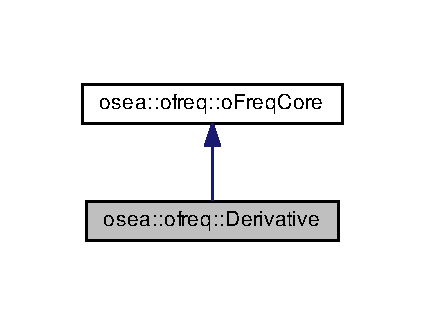
\includegraphics[width=204pt]{classosea_1_1ofreq_1_1_derivative__inherit__graph}
\end{center}
\end{figure}


Collaboration diagram for osea\-:\-:ofreq\-:\-:Derivative\-:
\nopagebreak
\begin{figure}[H]
\begin{center}
\leavevmode
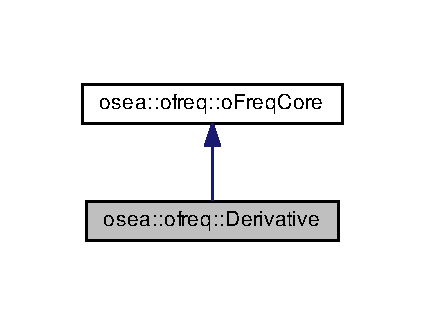
\includegraphics[width=204pt]{classosea_1_1ofreq_1_1_derivative__coll__graph}
\end{center}
\end{figure}
\subsection*{Public Member Functions}
\begin{DoxyCompactItemize}
\item 
\hyperlink{classosea_1_1ofreq_1_1_derivative_adc03ec3ad150bc0de66a3e7200cd368f}{Derivative} ()
\item 
\hyperlink{classosea_1_1ofreq_1_1_derivative_a7fc4ee53f460dfb98b3db2e9c9830cf9}{$\sim$\-Derivative} ()
\item 
std\-::vector$<$ \hyperlink{classosea_1_1ofreq_1_1_equation}{Equation} $>$ \& \hyperlink{classosea_1_1ofreq_1_1_derivative_a7fa63ee738fcafcf3fccb796da095946}{list\-Equation} ()
\begin{DoxyCompactList}\small\item\em The list of equations. \end{DoxyCompactList}\item 
\hyperlink{classosea_1_1ofreq_1_1_equation}{Equation} \& \hyperlink{classosea_1_1ofreq_1_1_derivative_a432dcf928635e6f77801ae7b546656fe}{ref\-Index\-Equation} (int index\-In)
\begin{DoxyCompactList}\small\item\em Returns the equation requested. Only specified by the data index property of the equation object. \end{DoxyCompactList}\item 
\hyperlink{classosea_1_1ofreq_1_1_equation}{Equation} \hyperlink{classosea_1_1ofreq_1_1_derivative_af9b75e66d998bc3ad82250c6667d0c17}{get\-Index\-Equation} (int index\-In)
\begin{DoxyCompactList}\small\item\em Returns the equation requested. Only specified by the data index property of the equation object. \end{DoxyCompactList}\item 
\hyperlink{classosea_1_1ofreq_1_1_equation}{Equation} \& \hyperlink{classosea_1_1ofreq_1_1_derivative_a57fc9f8fc2bb6b416b9ade4f79f2bf1d}{list\-Equation} (unsigned int number)
\begin{DoxyCompactList}\small\item\em Retrieve the equation specified by the number. \end{DoxyCompactList}\item 
int \hyperlink{classosea_1_1ofreq_1_1_derivative_ac95af6fb993314a578b3f0d3cd57a9cc}{get\-Equation\-List\-Size} ()
\end{DoxyCompactItemize}
\subsection*{Additional Inherited Members}


\subsection{Detailed Description}
This class holds data for a derivative. 

\subsection{Constructor \& Destructor Documentation}
\hypertarget{classosea_1_1ofreq_1_1_derivative_adc03ec3ad150bc0de66a3e7200cd368f}{\index{osea\-::ofreq\-::\-Derivative@{osea\-::ofreq\-::\-Derivative}!Derivative@{Derivative}}
\index{Derivative@{Derivative}!osea::ofreq::Derivative@{osea\-::ofreq\-::\-Derivative}}
\subsubsection[{Derivative}]{\setlength{\rightskip}{0pt plus 5cm}Derivative\-::\-Derivative (
\begin{DoxyParamCaption}
{}
\end{DoxyParamCaption}
)}}\label{classosea_1_1ofreq_1_1_derivative_adc03ec3ad150bc0de66a3e7200cd368f}
This default constructor creates a \hyperlink{classosea_1_1ofreq_1_1_body}{Body} object. \hypertarget{classosea_1_1ofreq_1_1_derivative_a7fc4ee53f460dfb98b3db2e9c9830cf9}{\index{osea\-::ofreq\-::\-Derivative@{osea\-::ofreq\-::\-Derivative}!$\sim$\-Derivative@{$\sim$\-Derivative}}
\index{$\sim$\-Derivative@{$\sim$\-Derivative}!osea::ofreq::Derivative@{osea\-::ofreq\-::\-Derivative}}
\subsubsection[{$\sim$\-Derivative}]{\setlength{\rightskip}{0pt plus 5cm}Derivative\-::$\sim$\-Derivative (
\begin{DoxyParamCaption}
{}
\end{DoxyParamCaption}
)}}\label{classosea_1_1ofreq_1_1_derivative_a7fc4ee53f460dfb98b3db2e9c9830cf9}
The default destructor, nothing happens here. 

\subsection{Member Function Documentation}
\hypertarget{classosea_1_1ofreq_1_1_derivative_ac95af6fb993314a578b3f0d3cd57a9cc}{\index{osea\-::ofreq\-::\-Derivative@{osea\-::ofreq\-::\-Derivative}!get\-Equation\-List\-Size@{get\-Equation\-List\-Size}}
\index{get\-Equation\-List\-Size@{get\-Equation\-List\-Size}!osea::ofreq::Derivative@{osea\-::ofreq\-::\-Derivative}}
\subsubsection[{get\-Equation\-List\-Size}]{\setlength{\rightskip}{0pt plus 5cm}int Derivative\-::get\-Equation\-List\-Size (
\begin{DoxyParamCaption}
{}
\end{DoxyParamCaption}
)}}\label{classosea_1_1ofreq_1_1_derivative_ac95af6fb993314a578b3f0d3cd57a9cc}
Retrieve the size of the equation list. \begin{DoxyReturn}{Returns}
The size of the equation list. 
\end{DoxyReturn}
\hypertarget{classosea_1_1ofreq_1_1_derivative_af9b75e66d998bc3ad82250c6667d0c17}{\index{osea\-::ofreq\-::\-Derivative@{osea\-::ofreq\-::\-Derivative}!get\-Index\-Equation@{get\-Index\-Equation}}
\index{get\-Index\-Equation@{get\-Index\-Equation}!osea::ofreq::Derivative@{osea\-::ofreq\-::\-Derivative}}
\subsubsection[{get\-Index\-Equation}]{\setlength{\rightskip}{0pt plus 5cm}{\bf Equation} Derivative\-::get\-Index\-Equation (
\begin{DoxyParamCaption}
\item[{int}]{index\-In}
\end{DoxyParamCaption}
)}}\label{classosea_1_1ofreq_1_1_derivative_af9b75e66d998bc3ad82250c6667d0c17}


Returns the equation requested. Only specified by the data index property of the equation object. 

Returns the equation requested. Only specified by the data index property of the equation object. 
\begin{DoxyParams}{Parameters}
{\em index\-In} & The integer describing the data index for the equation requested. \\
\hline
\end{DoxyParams}
\begin{DoxyReturn}{Returns}
\hyperlink{classosea_1_1ofreq_1_1_equation}{Equation} object specified by the Data\-Index of index\-In. Value returned is by value. 
\end{DoxyReturn}
\hypertarget{classosea_1_1ofreq_1_1_derivative_a7fa63ee738fcafcf3fccb796da095946}{\index{osea\-::ofreq\-::\-Derivative@{osea\-::ofreq\-::\-Derivative}!list\-Equation@{list\-Equation}}
\index{list\-Equation@{list\-Equation}!osea::ofreq::Derivative@{osea\-::ofreq\-::\-Derivative}}
\subsubsection[{list\-Equation}]{\setlength{\rightskip}{0pt plus 5cm}vector$<$ {\bf Equation} $>$ \& Derivative\-::list\-Equation (
\begin{DoxyParamCaption}
{}
\end{DoxyParamCaption}
)}}\label{classosea_1_1ofreq_1_1_derivative_a7fa63ee738fcafcf3fccb796da095946}


The list of equations. 

Pointer to the list vector list of equations. Value returned by reference. \hypertarget{classosea_1_1ofreq_1_1_derivative_a57fc9f8fc2bb6b416b9ade4f79f2bf1d}{\index{osea\-::ofreq\-::\-Derivative@{osea\-::ofreq\-::\-Derivative}!list\-Equation@{list\-Equation}}
\index{list\-Equation@{list\-Equation}!osea::ofreq::Derivative@{osea\-::ofreq\-::\-Derivative}}
\subsubsection[{list\-Equation}]{\setlength{\rightskip}{0pt plus 5cm}{\bf Equation} \& Derivative\-::list\-Equation (
\begin{DoxyParamCaption}
\item[{unsigned int}]{number}
\end{DoxyParamCaption}
)}}\label{classosea_1_1ofreq_1_1_derivative_a57fc9f8fc2bb6b416b9ade4f79f2bf1d}


Retrieve the equation specified by the number. 

Retrieves the equation specified by the number. Value returned is a reference to the equation object. Allows editting of the equation object, or just data access. 
\begin{DoxyParams}{Parameters}
{\em number} & Integer representing which equation number should be returned. \\
\hline
\end{DoxyParams}
\begin{DoxyReturn}{Returns}
Value returned is a reference to the equation object. Allows editting of the equation object, or just data access. 
\end{DoxyReturn}
\hypertarget{classosea_1_1ofreq_1_1_derivative_a432dcf928635e6f77801ae7b546656fe}{\index{osea\-::ofreq\-::\-Derivative@{osea\-::ofreq\-::\-Derivative}!ref\-Index\-Equation@{ref\-Index\-Equation}}
\index{ref\-Index\-Equation@{ref\-Index\-Equation}!osea::ofreq::Derivative@{osea\-::ofreq\-::\-Derivative}}
\subsubsection[{ref\-Index\-Equation}]{\setlength{\rightskip}{0pt plus 5cm}{\bf Equation} \& Derivative\-::ref\-Index\-Equation (
\begin{DoxyParamCaption}
\item[{int}]{index\-In}
\end{DoxyParamCaption}
)}}\label{classosea_1_1ofreq_1_1_derivative_a432dcf928635e6f77801ae7b546656fe}


Returns the equation requested. Only specified by the data index property of the equation object. 

Returns the equation requested. Only specified by the data index property of the equation object. 
\begin{DoxyParams}{Parameters}
{\em index\-In} & The integer describing the data index for the equation requested. \\
\hline
\end{DoxyParams}
\begin{DoxyReturn}{Returns}
Pointer to the \hyperlink{classosea_1_1ofreq_1_1_equation}{Equation} object specified by the Data\-Index of index\-In. Value returned is by reference. 
\end{DoxyReturn}


The documentation for this class was generated from the following files\-:\begin{DoxyCompactItemize}
\item 
derivative.\-h\item 
derivative.\-cpp\end{DoxyCompactItemize}

\hypertarget{classosea_1_1ofreq_1_1dict_bodies}{\section{osea\-:\-:ofreq\-:\-:dict\-Bodies Class Reference}
\label{classosea_1_1ofreq_1_1dict_bodies}\index{osea\-::ofreq\-::dict\-Bodies@{osea\-::ofreq\-::dict\-Bodies}}
}


{\ttfamily \#include $<$dictbodies.\-h$>$}



Inheritance diagram for osea\-:\-:ofreq\-:\-:dict\-Bodies\-:
\nopagebreak
\begin{figure}[H]
\begin{center}
\leavevmode
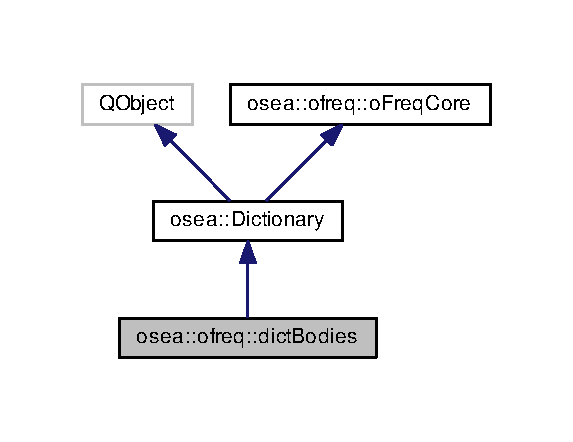
\includegraphics[width=275pt]{classosea_1_1ofreq_1_1dict_bodies__inherit__graph}
\end{center}
\end{figure}


Collaboration diagram for osea\-:\-:ofreq\-:\-:dict\-Bodies\-:
\nopagebreak
\begin{figure}[H]
\begin{center}
\leavevmode
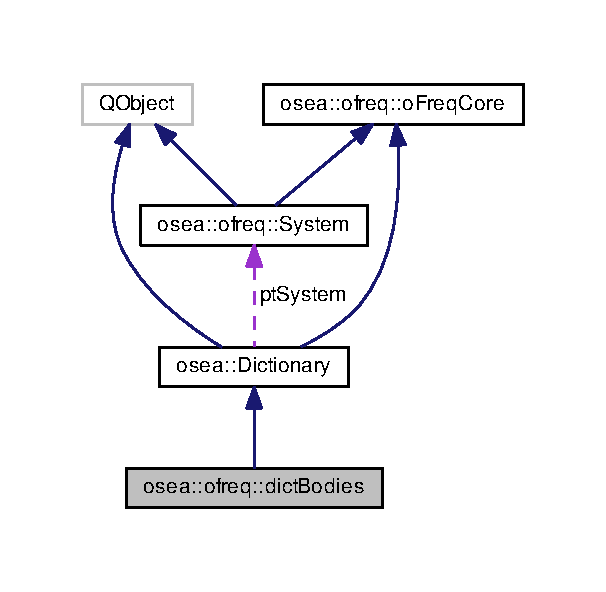
\includegraphics[width=291pt]{classosea_1_1ofreq_1_1dict_bodies__coll__graph}
\end{center}
\end{figure}
\subsection*{Protected Member Functions}
\begin{DoxyCompactItemize}
\item 
int \hyperlink{classosea_1_1ofreq_1_1dict_bodies_aff461cb5ceda5eee1a12da69aca94e1e}{define\-Key} (std\-::string key\-In, std\-::vector$<$ std\-::string $>$ val\-In)
\begin{DoxyCompactList}\small\item\em Function that defines how to interpret the key values. Contains a list of key names and corresponding actions to take for interpretting each key value. \end{DoxyCompactList}\item 
int \hyperlink{classosea_1_1ofreq_1_1dict_bodies_a3c00a8e8b6d24304cef35bcc50e7699b}{define\-Class} (std\-::string name\-In)
\begin{DoxyCompactList}\small\item\em Function that defines how to interpret the class name. Class name implies declaration of a new object of the class named by the class name. This is a separate set of definitions to handle class declarations. \end{DoxyCompactList}\end{DoxyCompactItemize}
\subsection*{Additional Inherited Members}


\subsection{Detailed Description}
The \hyperlink{classosea_1_1ofreq_1_1dict_bodies}{dict\-Bodies} class defines the key-\/word value pairs associated with the Bodies.\-in input file. Just as a normal dictionary defines the meaning of words, the \hyperlink{classosea_1_1ofreq_1_1dict_bodies}{dict\-Bodies} class works in the same way. The \hyperlink{classosea_1_1ofreq_1_1dict_bodies}{dict\-Bodies} class takes individual pairs of keywords and values. It has a definition for each of these keywords. The definition is whatever actions are necessary to process the value of key-\/pair and apply it to the program. This may include variable type conversions. It will also use slots and signals to retrieve pointers to any appropriate objects that the \hyperlink{classosea_1_1ofreq_1_1dict_bodies}{dict\-Bodies} object needs to interact with. It will use the properties of those objects to apply the values it finds in the key-\/value pair. Any objects created in the \hyperlink{classosea_1_1ofreq_1_1dict_bodies}{dict\-Bodies} class can be safely deleted once all file reading is done.

Note\-: The code for the \hyperlink{classosea_1_1ofreq_1_1dict_bodies}{dict\-Bodies} object always references the last object in the list. This assumes that no other commands get issued in the input file between the creation of an object and the definition of key-\/value pairs associated with that object. Currently, I can not imagine any situation where this assumption would be violated. But do consider this when planning error recovery methods. \begin{DoxySeeAlso}{See Also}
\hyperlink{classosea_1_1_dictionary}{Dictionary} 

\hyperlink{classosea_1_1_file_reader}{File\-Reader} 
\end{DoxySeeAlso}


\subsection{Member Function Documentation}
\hypertarget{classosea_1_1ofreq_1_1dict_bodies_a3c00a8e8b6d24304cef35bcc50e7699b}{\index{osea\-::ofreq\-::dict\-Bodies@{osea\-::ofreq\-::dict\-Bodies}!define\-Class@{define\-Class}}
\index{define\-Class@{define\-Class}!osea::ofreq::dictBodies@{osea\-::ofreq\-::dict\-Bodies}}
\subsubsection[{define\-Class}]{\setlength{\rightskip}{0pt plus 5cm}int dict\-Bodies\-::define\-Class (
\begin{DoxyParamCaption}
\item[{std\-::string}]{name\-In}
\end{DoxyParamCaption}
)\hspace{0.3cm}{\ttfamily [protected]}, {\ttfamily [virtual]}}}\label{classosea_1_1ofreq_1_1dict_bodies_a3c00a8e8b6d24304cef35bcc50e7699b}


Function that defines how to interpret the class name. Class name implies declaration of a new object of the class named by the class name. This is a separate set of definitions to handle class declarations. 


\begin{DoxyParams}{Parameters}
{\em name\-In} & std\-::string, variable passed by value. The name of the class name. \\
\hline
\end{DoxyParams}
\begin{DoxyReturn}{Returns}
Returns status of assigning key. Returned value is an integer, passed by value. See list of return codes below\-: 0\-: Key definition found. Success. 1\-: No key found. / General error message. 2\-: Key is invalid within current active object. 99\-: Function virtual definition only. Not currently defined. 
\end{DoxyReturn}


Reimplemented from \hyperlink{classosea_1_1_dictionary_a42843f64aa966b8c686d9e3750cbdb4b}{osea\-::\-Dictionary}.

\hypertarget{classosea_1_1ofreq_1_1dict_bodies_aff461cb5ceda5eee1a12da69aca94e1e}{\index{osea\-::ofreq\-::dict\-Bodies@{osea\-::ofreq\-::dict\-Bodies}!define\-Key@{define\-Key}}
\index{define\-Key@{define\-Key}!osea::ofreq::dictBodies@{osea\-::ofreq\-::dict\-Bodies}}
\subsubsection[{define\-Key}]{\setlength{\rightskip}{0pt plus 5cm}int dict\-Bodies\-::define\-Key (
\begin{DoxyParamCaption}
\item[{std\-::string}]{key\-In, }
\item[{std\-::vector$<$ std\-::string $>$}]{val\-In}
\end{DoxyParamCaption}
)\hspace{0.3cm}{\ttfamily [protected]}, {\ttfamily [virtual]}}}\label{classosea_1_1ofreq_1_1dict_bodies_aff461cb5ceda5eee1a12da69aca94e1e}


Function that defines how to interpret the key values. Contains a list of key names and corresponding actions to take for interpretting each key value. 


\begin{DoxyParams}{Parameters}
{\em key\-In} & std\-::string containing the key name. Variable passed by value. \\
\hline
{\em val\-In} & Vector of strings containing the key values. Variable passed by value. \\
\hline
\end{DoxyParams}
\begin{DoxyReturn}{Returns}
Returns status of assigning key. Returned value is an integer, passed by value. See list of return codes below\-: 0\-: Key definition found. Success. 1\-: No key found. / General error message. 2\-: Key is invalid within current active object. 99\-: Function virtual definition only. Not currently defined. 
\end{DoxyReturn}


Reimplemented from \hyperlink{classosea_1_1_dictionary_ae96470181c8b1762204493fa45e96d7c}{osea\-::\-Dictionary}.



The documentation for this class was generated from the following files\-:\begin{DoxyCompactItemize}
\item 
dictbodies.\-h\item 
dictbodies.\-cpp\end{DoxyCompactItemize}

\hypertarget{classosea_1_1ofreq_1_1dict_control}{\section{osea\-:\-:ofreq\-:\-:dict\-Control Class Reference}
\label{classosea_1_1ofreq_1_1dict_control}\index{osea\-::ofreq\-::dict\-Control@{osea\-::ofreq\-::dict\-Control}}
}


{\ttfamily \#include $<$dictcontrol.\-h$>$}



Inheritance diagram for osea\-:\-:ofreq\-:\-:dict\-Control\-:\nopagebreak
\begin{figure}[H]
\begin{center}
\leavevmode
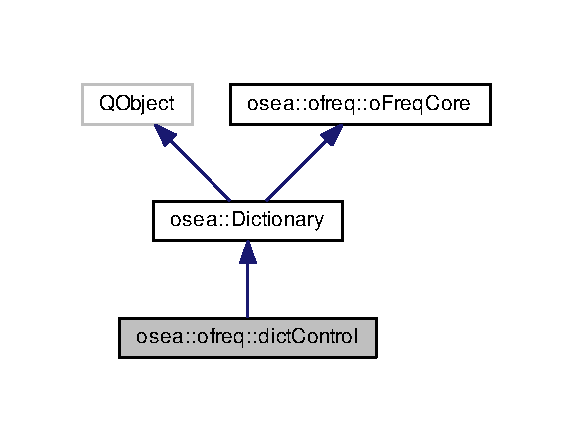
\includegraphics[width=275pt]{classosea_1_1ofreq_1_1dict_control__inherit__graph}
\end{center}
\end{figure}


Collaboration diagram for osea\-:\-:ofreq\-:\-:dict\-Control\-:\nopagebreak
\begin{figure}[H]
\begin{center}
\leavevmode
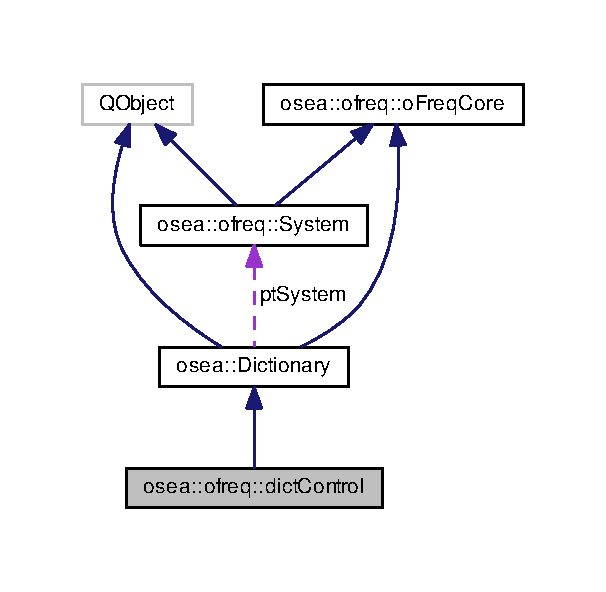
\includegraphics[width=291pt]{classosea_1_1ofreq_1_1dict_control__coll__graph}
\end{center}
\end{figure}
\subsection*{Protected Member Functions}
\begin{DoxyCompactItemize}
\item 
int \hyperlink{classosea_1_1ofreq_1_1dict_control_a048421f7c1bc9b8a023a159c59407bb9}{define\-Key} (std\-::string key\-In, std\-::vector$<$ std\-::string $>$ val\-In)
\begin{DoxyCompactList}\small\item\em Function that defines how to interpret the key values. Contains a list of key names and corresponding actions to take for interpretting each key value. \end{DoxyCompactList}\item 
int \hyperlink{classosea_1_1ofreq_1_1dict_control_a8c9cbaf3a2d4601dca4ad74667594a9e}{define\-Class} (std\-::string name\-In)
\begin{DoxyCompactList}\small\item\em Function that defines how to interpret the class name. Class name implies declaration of a new object of the class named by the class name. This is a separate set of definitions to handle class declarations. \end{DoxyCompactList}\end{DoxyCompactItemize}
\subsection*{Additional Inherited Members}


\subsection{Detailed Description}
The \hyperlink{classosea_1_1ofreq_1_1dict_control}{dict\-Control} class defines the key-\/word value pairs associated with the Control.\-in input file. Just as a normal dictionary defines the meaning of words, the \hyperlink{classosea_1_1ofreq_1_1dict_control}{dict\-Control} class works in the same way. The \hyperlink{classosea_1_1ofreq_1_1dict_control}{dict\-Control} class takes individual pairs of keywords and values. It has a definition for each of these keywords. The definition is whatever actions are necessary to process the value of key-\/pair and apply it to the program. This may include variable type conversions. It will also use slots and signals to retrieve pointers to any appropriate objects that the \hyperlink{classosea_1_1ofreq_1_1dict_control}{dict\-Control} object needs to interact with. It will use the properties of those objects to apply the values it finds in the key-\/value pair. Any objects created in the \hyperlink{classosea_1_1ofreq_1_1dict_control}{dict\-Control} object can be safely deleted once all file reading is done. \begin{DoxySeeAlso}{See Also}
\hyperlink{classosea_1_1_dictionary}{Dictionary} 

\hyperlink{classosea_1_1_file_reader}{File\-Reader} 
\end{DoxySeeAlso}


\subsection{Member Function Documentation}
\hypertarget{classosea_1_1ofreq_1_1dict_control_a8c9cbaf3a2d4601dca4ad74667594a9e}{\index{osea\-::ofreq\-::dict\-Control@{osea\-::ofreq\-::dict\-Control}!define\-Class@{define\-Class}}
\index{define\-Class@{define\-Class}!osea::ofreq::dictControl@{osea\-::ofreq\-::dict\-Control}}
\subsubsection[{define\-Class}]{\setlength{\rightskip}{0pt plus 5cm}int dict\-Control\-::define\-Class (
\begin{DoxyParamCaption}
\item[{std\-::string}]{name\-In}
\end{DoxyParamCaption}
)\hspace{0.3cm}{\ttfamily [protected]}, {\ttfamily [virtual]}}}\label{classosea_1_1ofreq_1_1dict_control_a8c9cbaf3a2d4601dca4ad74667594a9e}


Function that defines how to interpret the class name. Class name implies declaration of a new object of the class named by the class name. This is a separate set of definitions to handle class declarations. 


\begin{DoxyParams}{Parameters}
{\em name\-In} & std\-::string, variable passed by value. The name of the class name. \\
\hline
\end{DoxyParams}
\begin{DoxyReturn}{Returns}
Returns status of assigning key. Returned value is an integer, passed by value. See list of return codes below\-: 0\-: Key definition found. Success. 1\-: No key found. / General error message. 2\-: Key is invalid within current active object. 99\-: Function virtual definition only. Not currently defined. 
\end{DoxyReturn}


Reimplemented from \hyperlink{classosea_1_1_dictionary_a42843f64aa966b8c686d9e3750cbdb4b}{osea\-::\-Dictionary}.

\hypertarget{classosea_1_1ofreq_1_1dict_control_a048421f7c1bc9b8a023a159c59407bb9}{\index{osea\-::ofreq\-::dict\-Control@{osea\-::ofreq\-::dict\-Control}!define\-Key@{define\-Key}}
\index{define\-Key@{define\-Key}!osea::ofreq::dictControl@{osea\-::ofreq\-::dict\-Control}}
\subsubsection[{define\-Key}]{\setlength{\rightskip}{0pt plus 5cm}int dict\-Control\-::define\-Key (
\begin{DoxyParamCaption}
\item[{std\-::string}]{key\-In, }
\item[{std\-::vector$<$ std\-::string $>$}]{val\-In}
\end{DoxyParamCaption}
)\hspace{0.3cm}{\ttfamily [protected]}, {\ttfamily [virtual]}}}\label{classosea_1_1ofreq_1_1dict_control_a048421f7c1bc9b8a023a159c59407bb9}


Function that defines how to interpret the key values. Contains a list of key names and corresponding actions to take for interpretting each key value. 


\begin{DoxyParams}{Parameters}
{\em key\-In} & std\-::string containing the key name. Variable passed by value. \\
\hline
{\em val\-In} & Vector of strings containing the key values. Variable passed by value. \\
\hline
\end{DoxyParams}
\begin{DoxyReturn}{Returns}
Returns status of assigning key. Returned value is an integer, passed by value. See list of return codes below\-: 0\-: Key definition found. Success. 1\-: No key found. / General error message. 2\-: Key is invalid within current active object. 99\-: Function virtual definition only. Not currently defined. 
\end{DoxyReturn}


Reimplemented from \hyperlink{classosea_1_1_dictionary_ae96470181c8b1762204493fa45e96d7c}{osea\-::\-Dictionary}.



Here is the call graph for this function\-:\nopagebreak
\begin{figure}[H]
\begin{center}
\leavevmode
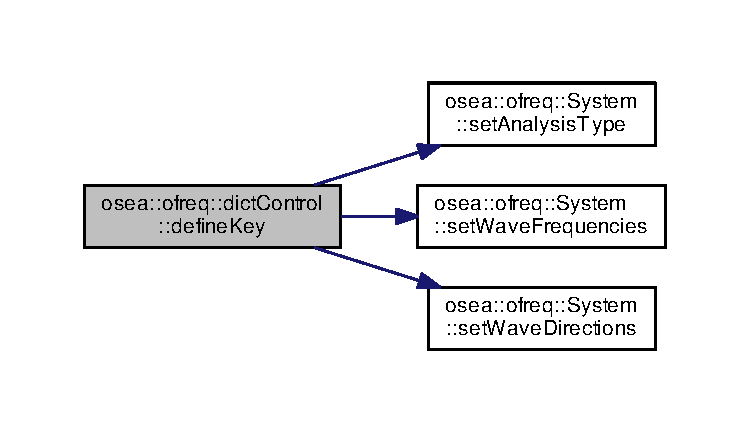
\includegraphics[width=350pt]{classosea_1_1ofreq_1_1dict_control_a048421f7c1bc9b8a023a159c59407bb9_cgraph}
\end{center}
\end{figure}




The documentation for this class was generated from the following files\-:\begin{DoxyCompactItemize}
\item 
dictcontrol.\-h\item 
dictcontrol.\-cpp\end{DoxyCompactItemize}

\hypertarget{classosea_1_1ofreq_1_1dict_forces}{\section{osea\-:\-:ofreq\-:\-:dict\-Forces Class Reference}
\label{classosea_1_1ofreq_1_1dict_forces}\index{osea\-::ofreq\-::dict\-Forces@{osea\-::ofreq\-::dict\-Forces}}
}


{\ttfamily \#include $<$dictforces.\-h$>$}



Inheritance diagram for osea\-:\-:ofreq\-:\-:dict\-Forces\-:
\nopagebreak
\begin{figure}[H]
\begin{center}
\leavevmode
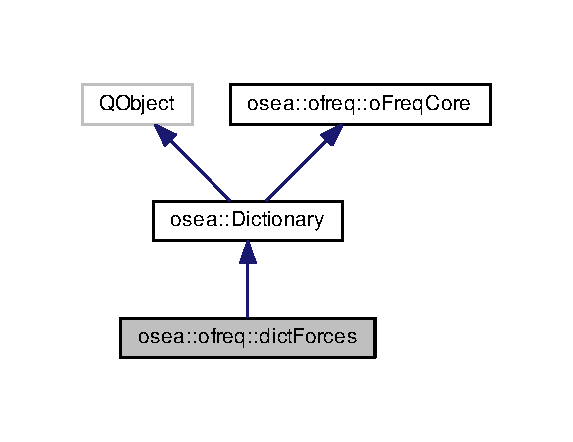
\includegraphics[width=286pt]{classosea_1_1ofreq_1_1dict_forces__inherit__graph}
\end{center}
\end{figure}
\subsection*{Public Member Functions}
\begin{DoxyCompactItemize}
\item 
\hyperlink{classosea_1_1ofreq_1_1dict_forces_ae9af9b8247c5b69d3041167ff1f898c6}{dict\-Forces} ()
\end{DoxyCompactItemize}
\subsection*{Protected Member Functions}
\begin{DoxyCompactItemize}
\item 
int \hyperlink{classosea_1_1ofreq_1_1dict_forces_ad2aef64f85e81b8b070ae732d757237e}{define\-Key} (std\-::string key\-In, std\-::vector$<$ std\-::string $>$ val\-In)
\begin{DoxyCompactList}\small\item\em Function that defines how to interpret the key values. Contains a list of key names and corresponding actions to take for interpretting each key value. \end{DoxyCompactList}\item 
int \hyperlink{classosea_1_1ofreq_1_1dict_forces_a4e1fd8cea0c9c689daf6eed864073485}{define\-Class} (std\-::string name\-In)
\begin{DoxyCompactList}\small\item\em Function that defines how to interpret the class name. Class name implies declaration of a new object of the class named by the class name. This is a separate set of definitions to handle class declarations. \end{DoxyCompactList}\end{DoxyCompactItemize}
\subsection*{Additional Inherited Members}


\subsection{Detailed Description}
The \hyperlink{classosea_1_1ofreq_1_1dict_forces}{dict\-Forces} class defines the key-\/word value pairs associated with the Forces.\-in input file. Just as a normal dictionary defines the meaning of words, the \hyperlink{classosea_1_1ofreq_1_1dict_forces}{dict\-Forces} class works in the same way. The \hyperlink{classosea_1_1ofreq_1_1dict_forces}{dict\-Forces} class takes individual pairs of keywords and values. It has a definition for each of these keywords. The definition is whatever actions are necessary to process the value of key-\/pair and apply it to the program. This may include variable type conversions. It will also use slots and signals to retrieve pointers to any appropriate objects that the \hyperlink{classosea_1_1ofreq_1_1dict_forces}{dict\-Forces} object needs to interact with. It will use the properties of those objects to apply the values it finds in the key-\/value pair. Any objects created in the \hyperlink{classosea_1_1ofreq_1_1dict_forces}{dict\-Forces} class can be safely deleted once all file reading is done.

Note\-: The code for the \hyperlink{classosea_1_1ofreq_1_1dict_forces}{dict\-Forces} object always references the last object in the list. This assumes that no other commands get issued in the input file between the creation of an object and the definition of key-\/value pairs associated with that object. Currently, I can not imagine any situation where this assumption would be violated. But do consider this when planning error recovery methods. \begin{DoxySeeAlso}{See Also}
\hyperlink{classosea_1_1_dictionary}{Dictionary} 

\hyperlink{classosea_1_1_file_reader}{File\-Reader} 
\end{DoxySeeAlso}


Definition at line 98 of file dictforces.\-h.



\subsection{Constructor \& Destructor Documentation}
\hypertarget{classosea_1_1ofreq_1_1dict_forces_ae9af9b8247c5b69d3041167ff1f898c6}{\index{osea\-::ofreq\-::dict\-Forces@{osea\-::ofreq\-::dict\-Forces}!dict\-Forces@{dict\-Forces}}
\index{dict\-Forces@{dict\-Forces}!osea::ofreq::dictForces@{osea\-::ofreq\-::dict\-Forces}}
\subsubsection[{dict\-Forces}]{\setlength{\rightskip}{0pt plus 5cm}dict\-Forces\-::dict\-Forces (
\begin{DoxyParamCaption}
{}
\end{DoxyParamCaption}
)}}\label{classosea_1_1ofreq_1_1dict_forces_ae9af9b8247c5b69d3041167ff1f898c6}


Definition at line 57 of file dictforces.\-cpp.



\subsection{Member Function Documentation}
\hypertarget{classosea_1_1ofreq_1_1dict_forces_a4e1fd8cea0c9c689daf6eed864073485}{\index{osea\-::ofreq\-::dict\-Forces@{osea\-::ofreq\-::dict\-Forces}!define\-Class@{define\-Class}}
\index{define\-Class@{define\-Class}!osea::ofreq::dictForces@{osea\-::ofreq\-::dict\-Forces}}
\subsubsection[{define\-Class}]{\setlength{\rightskip}{0pt plus 5cm}int dict\-Forces\-::define\-Class (
\begin{DoxyParamCaption}
\item[{std\-::string}]{name\-In}
\end{DoxyParamCaption}
)\hspace{0.3cm}{\ttfamily [protected]}, {\ttfamily [virtual]}}}\label{classosea_1_1ofreq_1_1dict_forces_a4e1fd8cea0c9c689daf6eed864073485}


Function that defines how to interpret the class name. Class name implies declaration of a new object of the class named by the class name. This is a separate set of definitions to handle class declarations. 


\begin{DoxyParams}{Parameters}
{\em name\-In} & std\-::string, variable passed by value. The name of the class name. \\
\hline
\end{DoxyParams}
\begin{DoxyReturn}{Returns}
Returns status of assigning key. Returned value is an integer, passed by value. See list of return codes below\-: 0\-: Key definition found. Success. 1\-: No key found. / General error message. 2\-: Key is invalid within current active object. 99\-: Function virtual definition only. Not currently defined. 
\end{DoxyReturn}


Reimplemented from \hyperlink{classosea_1_1_dictionary_a42843f64aa966b8c686d9e3750cbdb4b}{osea\-::\-Dictionary}.



Definition at line 203 of file dictforces.\-cpp.

\hypertarget{classosea_1_1ofreq_1_1dict_forces_ad2aef64f85e81b8b070ae732d757237e}{\index{osea\-::ofreq\-::dict\-Forces@{osea\-::ofreq\-::dict\-Forces}!define\-Key@{define\-Key}}
\index{define\-Key@{define\-Key}!osea::ofreq::dictForces@{osea\-::ofreq\-::dict\-Forces}}
\subsubsection[{define\-Key}]{\setlength{\rightskip}{0pt plus 5cm}int dict\-Forces\-::define\-Key (
\begin{DoxyParamCaption}
\item[{std\-::string}]{key\-In, }
\item[{std\-::vector$<$ std\-::string $>$}]{val\-In}
\end{DoxyParamCaption}
)\hspace{0.3cm}{\ttfamily [protected]}, {\ttfamily [virtual]}}}\label{classosea_1_1ofreq_1_1dict_forces_ad2aef64f85e81b8b070ae732d757237e}


Function that defines how to interpret the key values. Contains a list of key names and corresponding actions to take for interpretting each key value. 


\begin{DoxyParams}{Parameters}
{\em key\-In} & std\-::string containing the key name. Variable passed by value. \\
\hline
{\em val\-In} & Vector of strings containing the key values. Variable passed by value. \\
\hline
\end{DoxyParams}
\begin{DoxyReturn}{Returns}
Returns status of assigning key. Returned value is an integer, passed by value. See list of return codes below\-: 0\-: Key definition found. Success. 1\-: No key found. / General error message. 2\-: Key is invalid within current active object. 99\-: Function virtual definition only. Not currently defined. 
\end{DoxyReturn}


Reimplemented from \hyperlink{classosea_1_1_dictionary_ae96470181c8b1762204493fa45e96d7c}{osea\-::\-Dictionary}.



Definition at line 71 of file dictforces.\-cpp.



The documentation for this class was generated from the following files\-:\begin{DoxyCompactItemize}
\item 
/home/\-Ship\-\_\-\-Design/\-Projects/\-D\-M\-S1305 Open\-S\-E\-A/master/200\-\_\-src/bin/ofreq/file\-\_\-reader/\hyperlink{dictforces_8h}{dictforces.\-h}\item 
/home/\-Ship\-\_\-\-Design/\-Projects/\-D\-M\-S1305 Open\-S\-E\-A/master/200\-\_\-src/bin/ofreq/file\-\_\-reader/\hyperlink{dictforces_8cpp}{dictforces.\-cpp}\end{DoxyCompactItemize}

\hypertarget{classosea_1_1_dictionary}{\section{osea\-:\-:Dictionary Class Reference}
\label{classosea_1_1_dictionary}\index{osea\-::\-Dictionary@{osea\-::\-Dictionary}}
}


{\ttfamily \#include $<$dictionary.\-h$>$}



Inheritance diagram for osea\-:\-:Dictionary\-:\nopagebreak
\begin{figure}[H]
\begin{center}
\leavevmode
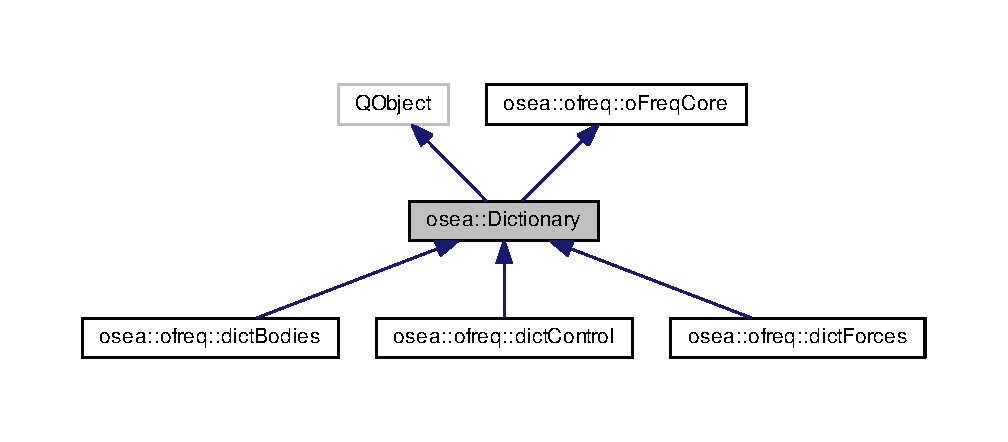
\includegraphics[width=350pt]{classosea_1_1_dictionary__inherit__graph}
\end{center}
\end{figure}
\subsection*{Public Slots}
\begin{DoxyCompactItemize}
\item 
virtual void \hyperlink{classosea_1_1_dictionary_a900221a385d133644aedcadbae90c2be}{set\-Object} (\hyperlink{classosea_1_1_object_group}{Object\-Group} input)
\begin{DoxyCompactList}\small\item\em Public signal for the \hyperlink{classosea_1_1_object_group}{Object\-Group} object that is sent to the \hyperlink{classosea_1_1_dictionary}{Dictionary} object for procesing. \end{DoxyCompactList}\item 
virtual void \hyperlink{classosea_1_1_dictionary_a4f5b4ce990794a633ff8b69b8c021b66}{set\-System} (\hyperlink{classosea_1_1ofreq_1_1_system}{ofreq\-::\-System} $\ast$pt\-Input)
\begin{DoxyCompactList}\small\item\em Sets the system object for the dictionary to reference. \end{DoxyCompactList}\end{DoxyCompactItemize}
\subsection*{Public Member Functions}
\begin{DoxyCompactItemize}
\item 
\hyperlink{classosea_1_1_dictionary_a6ff9dd5005c8796e0cc13a8bc4cb2288}{Dictionary} (Q\-Object $\ast$parent)
\item 
\hyperlink{classosea_1_1_dictionary_aee8d612bc9d323c38faba045ba384b8b}{Dictionary} ()
\end{DoxyCompactItemize}
\subsection*{Protected Member Functions}
\begin{DoxyCompactItemize}
\item 
virtual int \hyperlink{classosea_1_1_dictionary_ae96470181c8b1762204493fa45e96d7c}{define\-Key} (std\-::string key\-In, std\-::vector$<$ std\-::string $>$ val\-In)
\begin{DoxyCompactList}\small\item\em Pure virtual function that defines how to interpret the key values. Contains a list of key names and corresponding actions to take for interpretting each key value. \end{DoxyCompactList}\item 
virtual int \hyperlink{classosea_1_1_dictionary_a42843f64aa966b8c686d9e3750cbdb4b}{define\-Class} (std\-::string name\-In)
\begin{DoxyCompactList}\small\item\em Pure virtual function that defines how to interpret the class name. Class name implies declaration of a new object of the class named by the class name. This is a separate set of definitions to handle class declarations. \end{DoxyCompactList}\item 
std\-::complex$<$ double $>$ \hyperlink{classosea_1_1_dictionary_ac714952a7fcf99ab69de015c606322ad}{convert\-Complex} (std\-::string input)
\begin{DoxyCompactList}\small\item\em Converts a std\-::string of a complex number into a complex object (double base type) i.\-e. std\-::complex$<$double$>$. \end{DoxyCompactList}\end{DoxyCompactItemize}
\subsection*{Protected Attributes}
\begin{DoxyCompactItemize}
\item 
\hyperlink{classosea_1_1ofreq_1_1_system}{ofreq\-::\-System} $\ast$ \hyperlink{classosea_1_1_dictionary_a72bf4127a7ee1fb2b784abb6df020fed}{pt\-System}
\begin{DoxyCompactList}\small\item\em Pointer to the System object. Used to reference any important variables in the System object. \end{DoxyCompactList}\end{DoxyCompactItemize}
\subsection*{Additional Inherited Members}


\subsection{Detailed Description}
This is a virtual class definition, inheritted by each file\-Dictionary object. Contains the basic functions for how to recursively progress through the definitions for an \hyperlink{classosea_1_1_object_group}{Object\-Group} object that is fed in. \begin{DoxySeeAlso}{See Also}
\hyperlink{classosea_1_1_object_group}{Object\-Group} 
\end{DoxySeeAlso}


Definition at line 84 of file dictionary.\-h.



\subsection{Constructor \& Destructor Documentation}
\hypertarget{classosea_1_1_dictionary_a6ff9dd5005c8796e0cc13a8bc4cb2288}{\index{osea\-::\-Dictionary@{osea\-::\-Dictionary}!Dictionary@{Dictionary}}
\index{Dictionary@{Dictionary}!osea::Dictionary@{osea\-::\-Dictionary}}
\subsubsection[{Dictionary}]{\setlength{\rightskip}{0pt plus 5cm}Dictionary\-::\-Dictionary (
\begin{DoxyParamCaption}
\item[{Q\-Object $\ast$}]{parent}
\end{DoxyParamCaption}
)\hspace{0.3cm}{\ttfamily [explicit]}}}\label{classosea_1_1_dictionary_a6ff9dd5005c8796e0cc13a8bc4cb2288}


Definition at line 36 of file dictionary.\-cpp.

\hypertarget{classosea_1_1_dictionary_aee8d612bc9d323c38faba045ba384b8b}{\index{osea\-::\-Dictionary@{osea\-::\-Dictionary}!Dictionary@{Dictionary}}
\index{Dictionary@{Dictionary}!osea::Dictionary@{osea\-::\-Dictionary}}
\subsubsection[{Dictionary}]{\setlength{\rightskip}{0pt plus 5cm}Dictionary\-::\-Dictionary (
\begin{DoxyParamCaption}
{}
\end{DoxyParamCaption}
)}}\label{classosea_1_1_dictionary_aee8d612bc9d323c38faba045ba384b8b}


Definition at line 42 of file dictionary.\-cpp.



\subsection{Member Function Documentation}
\hypertarget{classosea_1_1_dictionary_ac714952a7fcf99ab69de015c606322ad}{\index{osea\-::\-Dictionary@{osea\-::\-Dictionary}!convert\-Complex@{convert\-Complex}}
\index{convert\-Complex@{convert\-Complex}!osea::Dictionary@{osea\-::\-Dictionary}}
\subsubsection[{convert\-Complex}]{\setlength{\rightskip}{0pt plus 5cm}complex$<$ double $>$ Dictionary\-::convert\-Complex (
\begin{DoxyParamCaption}
\item[{std\-::string}]{input}
\end{DoxyParamCaption}
)\hspace{0.3cm}{\ttfamily [protected]}}}\label{classosea_1_1_dictionary_ac714952a7fcf99ab69de015c606322ad}


Converts a std\-::string of a complex number into a complex object (double base type) i.\-e. std\-::complex$<$double$>$. 


\begin{DoxyParams}{Parameters}
{\em input} & The std\-::string which holds the complex number. Valid input formats are\-: 1.\-00+1.00i 1.\-00-\/1.\-00i 1.\-00+i1.00 1.\-00-\/i1.\-00 1.\-414$<$0.\-785398 (angle must be in radians) 1.\-414$<$-\/0.\-785398 (angle must be in radians) \\
\hline
\end{DoxyParams}
\begin{DoxyReturn}{Returns}
Returns a std\-::complex$<$double$>$ object. Variable passed by value. 
\end{DoxyReturn}


Definition at line 105 of file dictionary.\-cpp.

\hypertarget{classosea_1_1_dictionary_a42843f64aa966b8c686d9e3750cbdb4b}{\index{osea\-::\-Dictionary@{osea\-::\-Dictionary}!define\-Class@{define\-Class}}
\index{define\-Class@{define\-Class}!osea::Dictionary@{osea\-::\-Dictionary}}
\subsubsection[{define\-Class}]{\setlength{\rightskip}{0pt plus 5cm}int Dictionary\-::define\-Class (
\begin{DoxyParamCaption}
\item[{std\-::string}]{name\-In}
\end{DoxyParamCaption}
)\hspace{0.3cm}{\ttfamily [protected]}, {\ttfamily [virtual]}}}\label{classosea_1_1_dictionary_a42843f64aa966b8c686d9e3750cbdb4b}


Pure virtual function that defines how to interpret the class name. Class name implies declaration of a new object of the class named by the class name. This is a separate set of definitions to handle class declarations. 


\begin{DoxyParams}{Parameters}
{\em name\-In} & std\-::string, variable passed by value. The name of the class name. \\
\hline
\end{DoxyParams}
\begin{DoxyReturn}{Returns}
Returns status of assigning key. Returned value is an integer, passed by value. See list of return codes below\-: 0\-: Key definition found. Success. 1\-: No key found. / General error message. 2\-: Key is invalid within current active object. 99\-: Function virtual definition only. Not currently defined. 
\end{DoxyReturn}


Reimplemented in \hyperlink{classosea_1_1ofreq_1_1dict_bodies_a3c00a8e8b6d24304cef35bcc50e7699b}{osea\-::ofreq\-::dict\-Bodies}, \hyperlink{classosea_1_1ofreq_1_1dict_forces_a4e1fd8cea0c9c689daf6eed864073485}{osea\-::ofreq\-::dict\-Forces}, and \hyperlink{classosea_1_1ofreq_1_1dict_control_a8c9cbaf3a2d4601dca4ad74667594a9e}{osea\-::ofreq\-::dict\-Control}.



Definition at line 97 of file dictionary.\-cpp.

\hypertarget{classosea_1_1_dictionary_ae96470181c8b1762204493fa45e96d7c}{\index{osea\-::\-Dictionary@{osea\-::\-Dictionary}!define\-Key@{define\-Key}}
\index{define\-Key@{define\-Key}!osea::Dictionary@{osea\-::\-Dictionary}}
\subsubsection[{define\-Key}]{\setlength{\rightskip}{0pt plus 5cm}int Dictionary\-::define\-Key (
\begin{DoxyParamCaption}
\item[{std\-::string}]{key\-In, }
\item[{std\-::vector$<$ std\-::string $>$}]{val\-In}
\end{DoxyParamCaption}
)\hspace{0.3cm}{\ttfamily [protected]}, {\ttfamily [virtual]}}}\label{classosea_1_1_dictionary_ae96470181c8b1762204493fa45e96d7c}


Pure virtual function that defines how to interpret the key values. Contains a list of key names and corresponding actions to take for interpretting each key value. 


\begin{DoxyParams}{Parameters}
{\em key\-In} & std\-::string containing the key name. Variable passed by value. \\
\hline
{\em val\-In} & Vector of strings containing the key values. Variable passed by value. \\
\hline
\end{DoxyParams}
\begin{DoxyReturn}{Returns}
Returns status of assigning key. Returned value is an integer, passed by value. See list of return codes below\-: 0\-: Key definition found. Success. 1\-: No key found. / General error message. 2\-: Key is invalid within current active object. 99\-: Function virtual definition only. Not currently defined. 
\end{DoxyReturn}


Reimplemented in \hyperlink{classosea_1_1ofreq_1_1dict_bodies_aff461cb5ceda5eee1a12da69aca94e1e}{osea\-::ofreq\-::dict\-Bodies}, \hyperlink{classosea_1_1ofreq_1_1dict_forces_ad2aef64f85e81b8b070ae732d757237e}{osea\-::ofreq\-::dict\-Forces}, and \hyperlink{classosea_1_1ofreq_1_1dict_control_a048421f7c1bc9b8a023a159c59407bb9}{osea\-::ofreq\-::dict\-Control}.



Definition at line 89 of file dictionary.\-cpp.

\hypertarget{classosea_1_1_dictionary_a900221a385d133644aedcadbae90c2be}{\index{osea\-::\-Dictionary@{osea\-::\-Dictionary}!set\-Object@{set\-Object}}
\index{set\-Object@{set\-Object}!osea::Dictionary@{osea\-::\-Dictionary}}
\subsubsection[{set\-Object}]{\setlength{\rightskip}{0pt plus 5cm}void Dictionary\-::set\-Object (
\begin{DoxyParamCaption}
\item[{{\bf Object\-Group}}]{input}
\end{DoxyParamCaption}
)\hspace{0.3cm}{\ttfamily [virtual]}, {\ttfamily [slot]}}}\label{classosea_1_1_dictionary_a900221a385d133644aedcadbae90c2be}


Public signal for the \hyperlink{classosea_1_1_object_group}{Object\-Group} object that is sent to the \hyperlink{classosea_1_1_dictionary}{Dictionary} object for procesing. 


\begin{DoxyParams}{Parameters}
{\em input} & The \hyperlink{classosea_1_1_object_group}{Object\-Group} object that contains the class definitions. Variable passed by value. \\
\hline
\end{DoxyParams}


Definition at line 54 of file dictionary.\-cpp.



Here is the call graph for this function\-:\nopagebreak
\begin{figure}[H]
\begin{center}
\leavevmode
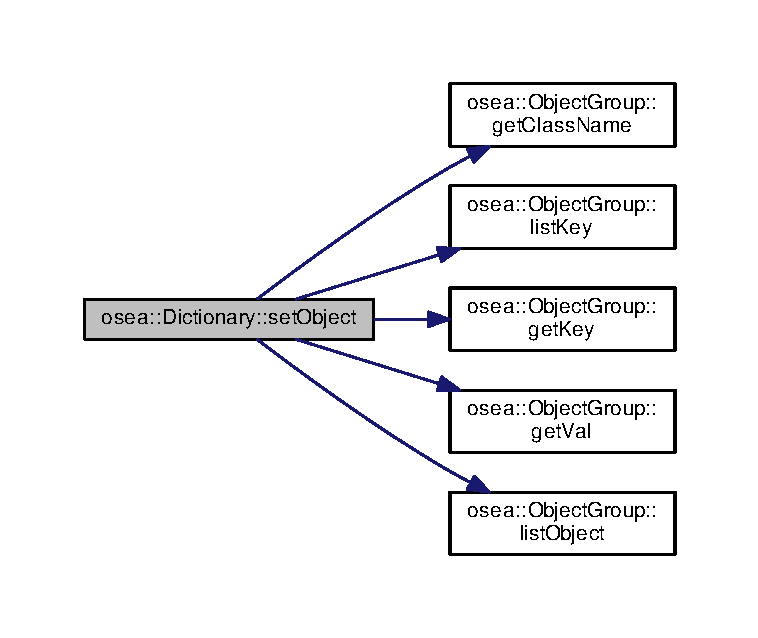
\includegraphics[width=350pt]{classosea_1_1_dictionary_a900221a385d133644aedcadbae90c2be_cgraph}
\end{center}
\end{figure}


\hypertarget{classosea_1_1_dictionary_a4f5b4ce990794a633ff8b69b8c021b66}{\index{osea\-::\-Dictionary@{osea\-::\-Dictionary}!set\-System@{set\-System}}
\index{set\-System@{set\-System}!osea::Dictionary@{osea\-::\-Dictionary}}
\subsubsection[{set\-System}]{\setlength{\rightskip}{0pt plus 5cm}void Dictionary\-::set\-System (
\begin{DoxyParamCaption}
\item[{{\bf ofreq\-::\-System} $\ast$}]{pt\-Input}
\end{DoxyParamCaption}
)\hspace{0.3cm}{\ttfamily [virtual]}, {\ttfamily [slot]}}}\label{classosea_1_1_dictionary_a4f5b4ce990794a633ff8b69b8c021b66}


Sets the system object for the dictionary to reference. 


\begin{DoxyParams}{Parameters}
{\em pt\-System} & Pointer to the System object. Variable passed by value. \\
\hline
\end{DoxyParams}


Definition at line 80 of file dictionary.\-cpp.



\subsection{Member Data Documentation}
\hypertarget{classosea_1_1_dictionary_a72bf4127a7ee1fb2b784abb6df020fed}{\index{osea\-::\-Dictionary@{osea\-::\-Dictionary}!pt\-System@{pt\-System}}
\index{pt\-System@{pt\-System}!osea::Dictionary@{osea\-::\-Dictionary}}
\subsubsection[{pt\-System}]{\setlength{\rightskip}{0pt plus 5cm}{\bf ofreq\-::\-System}$\ast$ osea\-::\-Dictionary\-::pt\-System\hspace{0.3cm}{\ttfamily [protected]}}}\label{classosea_1_1_dictionary_a72bf4127a7ee1fb2b784abb6df020fed}


Pointer to the System object. Used to reference any important variables in the System object. 



Definition at line 166 of file dictionary.\-h.



The documentation for this class was generated from the following files\-:\begin{DoxyCompactItemize}
\item 
/home/\-Ship\-\_\-\-Design/\-Projects/\-D\-M\-S1305 Open\-S\-E\-A/master/200\-\_\-src/bin/ofreq/file\-\_\-reader/\hyperlink{dictionary_8h}{dictionary.\-h}\item 
/home/\-Ship\-\_\-\-Design/\-Projects/\-D\-M\-S1305 Open\-S\-E\-A/master/200\-\_\-src/bin/ofreq/file\-\_\-reader/\hyperlink{dictionary_8cpp}{dictionary.\-cpp}\end{DoxyCompactItemize}

\hypertarget{classosea_1_1ofreq_1_1_equation}{\section{osea\-:\-:ofreq\-:\-:Equation Class Reference}
\label{classosea_1_1ofreq_1_1_equation}\index{osea\-::ofreq\-::\-Equation@{osea\-::ofreq\-::\-Equation}}
}


{\ttfamily \#include $<$equation.\-h$>$}



Inheritance diagram for osea\-:\-:ofreq\-:\-:Equation\-:\nopagebreak
\begin{figure}[H]
\begin{center}
\leavevmode
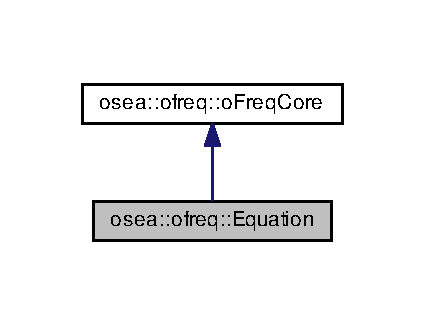
\includegraphics[width=204pt]{classosea_1_1ofreq_1_1_equation__inherit__graph}
\end{center}
\end{figure}


Collaboration diagram for osea\-:\-:ofreq\-:\-:Equation\-:\nopagebreak
\begin{figure}[H]
\begin{center}
\leavevmode
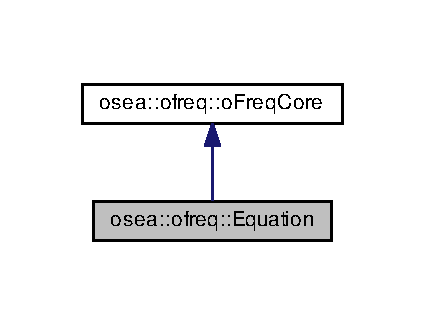
\includegraphics[width=204pt]{classosea_1_1ofreq_1_1_equation__coll__graph}
\end{center}
\end{figure}
\subsection*{Public Member Functions}
\begin{DoxyCompactItemize}
\item 
\hyperlink{classosea_1_1ofreq_1_1_equation_a68511fc719250ed80f86c50de9136733}{Equation} ()
\item 
\hyperlink{classosea_1_1ofreq_1_1_equation_a37fec641aec75302c37590d191421790}{Equation} (int Index\-In)
\begin{DoxyCompactList}\small\item\em Constructor with setting the data index. \end{DoxyCompactList}\item 
\hyperlink{classosea_1_1ofreq_1_1_equation_a097243d0dfd608330fc91f115a0d15bb}{$\sim$\-Equation} ()
\item 
std\-::vector$<$ double $>$ \& \hyperlink{classosea_1_1ofreq_1_1_equation_a40be3415ddc7ebc7aa93829f3eb750f0}{list\-Coefficient} ()
\begin{DoxyCompactList}\small\item\em Direct access to the list of coefficients. \end{DoxyCompactList}\item 
double \& \hyperlink{classosea_1_1ofreq_1_1_equation_acce479a17f90df340bcf9cabf06258a2}{list\-Coefficient} (unsigned int index)
\begin{DoxyCompactList}\small\item\em Provides direct access to a coefficient from the list of coefficients. \end{DoxyCompactList}\item 
std\-::vector$<$ double $>$ \& \hyperlink{classosea_1_1ofreq_1_1_equation_a736b8cff2908ad73abad4ca4533b830d}{list\-Variable} ()
\begin{DoxyCompactList}\small\item\em Provides direct access to the list of coefficients. This is the same as the \hyperlink{classosea_1_1ofreq_1_1_equation_a40be3415ddc7ebc7aa93829f3eb750f0}{list\-Coefficient()} method, just under a different name. \end{DoxyCompactList}\item 
double \& \hyperlink{classosea_1_1ofreq_1_1_equation_a9d969fd44848f29f135213aaa520fabe}{list\-Variable} (unsigned int index)
\begin{DoxyCompactList}\small\item\em Provides direct access to a coefficient from the list of coefficients. \end{DoxyCompactList}\item 
double \hyperlink{classosea_1_1ofreq_1_1_equation_a6aa77458d50e80de2a31708756c7925b}{get\-Coefficient} (int number)
\begin{DoxyCompactList}\small\item\em Get the coefficient at the specified number. \end{DoxyCompactList}\item 
void \hyperlink{classosea_1_1ofreq_1_1_equation_a96dd6f24624703a1ff3ffb4d19a76582}{set\-Coefficient} (int number, double coeff\-In)
\begin{DoxyCompactList}\small\item\em Set the coefficient value at the specified index number. \end{DoxyCompactList}\item 
unsigned int \hyperlink{classosea_1_1ofreq_1_1_equation_aa3ceaac689d9cfef1a1b3123d8ec4027}{get\-Coefficient\-List\-Size} ()
\item 
void \hyperlink{classosea_1_1ofreq_1_1_equation_aa9e40c1cc6fb3cb030e9956663025a87}{set\-Data\-Index} (int index)
\begin{DoxyCompactList}\small\item\em Set the index number of any equation data that should be retrieved. \end{DoxyCompactList}\item 
int \hyperlink{classosea_1_1ofreq_1_1_equation_ac5fd13eba76ddbbf4813823fad4166e2}{get\-Data\-Index} ()
\begin{DoxyCompactList}\small\item\em Get the index number of any equation data that should be retrieved. \end{DoxyCompactList}\item 
int \& \hyperlink{classosea_1_1ofreq_1_1_equation_a5964477a42f3941a968f249b89742d73}{ref\-Data\-Index} ()
\begin{DoxyCompactList}\small\item\em Exposed access to the data access variable. \end{DoxyCompactList}\end{DoxyCompactItemize}
\subsection*{Additional Inherited Members}


\subsection{Detailed Description}
This class holds data for an equation. 

\subsection{Constructor \& Destructor Documentation}
\hypertarget{classosea_1_1ofreq_1_1_equation_a68511fc719250ed80f86c50de9136733}{\index{osea\-::ofreq\-::\-Equation@{osea\-::ofreq\-::\-Equation}!Equation@{Equation}}
\index{Equation@{Equation}!osea::ofreq::Equation@{osea\-::ofreq\-::\-Equation}}
\subsubsection[{Equation}]{\setlength{\rightskip}{0pt plus 5cm}Equation\-::\-Equation (
\begin{DoxyParamCaption}
{}
\end{DoxyParamCaption}
)}}\label{classosea_1_1ofreq_1_1_equation_a68511fc719250ed80f86c50de9136733}
This default constructor. \hypertarget{classosea_1_1ofreq_1_1_equation_a37fec641aec75302c37590d191421790}{\index{osea\-::ofreq\-::\-Equation@{osea\-::ofreq\-::\-Equation}!Equation@{Equation}}
\index{Equation@{Equation}!osea::ofreq::Equation@{osea\-::ofreq\-::\-Equation}}
\subsubsection[{Equation}]{\setlength{\rightskip}{0pt plus 5cm}Equation\-::\-Equation (
\begin{DoxyParamCaption}
\item[{int}]{Index\-In}
\end{DoxyParamCaption}
)}}\label{classosea_1_1ofreq_1_1_equation_a37fec641aec75302c37590d191421790}


Constructor with setting the data index. 

Constructor with setting the data index. 
\begin{DoxyParams}{Parameters}
{\em Index\-In} & The integer specifying the data index number. \\
\hline
\end{DoxyParams}
\hypertarget{classosea_1_1ofreq_1_1_equation_a097243d0dfd608330fc91f115a0d15bb}{\index{osea\-::ofreq\-::\-Equation@{osea\-::ofreq\-::\-Equation}!$\sim$\-Equation@{$\sim$\-Equation}}
\index{$\sim$\-Equation@{$\sim$\-Equation}!osea::ofreq::Equation@{osea\-::ofreq\-::\-Equation}}
\subsubsection[{$\sim$\-Equation}]{\setlength{\rightskip}{0pt plus 5cm}Equation\-::$\sim$\-Equation (
\begin{DoxyParamCaption}
{}
\end{DoxyParamCaption}
)}}\label{classosea_1_1ofreq_1_1_equation_a097243d0dfd608330fc91f115a0d15bb}
The default destructor, nothing happens here. 

\subsection{Member Function Documentation}
\hypertarget{classosea_1_1ofreq_1_1_equation_a6aa77458d50e80de2a31708756c7925b}{\index{osea\-::ofreq\-::\-Equation@{osea\-::ofreq\-::\-Equation}!get\-Coefficient@{get\-Coefficient}}
\index{get\-Coefficient@{get\-Coefficient}!osea::ofreq::Equation@{osea\-::ofreq\-::\-Equation}}
\subsubsection[{get\-Coefficient}]{\setlength{\rightskip}{0pt plus 5cm}double Equation\-::get\-Coefficient (
\begin{DoxyParamCaption}
\item[{int}]{number}
\end{DoxyParamCaption}
)}}\label{classosea_1_1ofreq_1_1_equation_a6aa77458d50e80de2a31708756c7925b}


Get the coefficient at the specified number. 


\begin{DoxyParams}{Parameters}
{\em number} & The index number of the coefficient to retrieve. \\
\hline
\end{DoxyParams}
\begin{DoxyReturn}{Returns}
Returns a double precision floating point number of the coefficient at the index specified by number. 
\end{DoxyReturn}
\hypertarget{classosea_1_1ofreq_1_1_equation_aa3ceaac689d9cfef1a1b3123d8ec4027}{\index{osea\-::ofreq\-::\-Equation@{osea\-::ofreq\-::\-Equation}!get\-Coefficient\-List\-Size@{get\-Coefficient\-List\-Size}}
\index{get\-Coefficient\-List\-Size@{get\-Coefficient\-List\-Size}!osea::ofreq::Equation@{osea\-::ofreq\-::\-Equation}}
\subsubsection[{get\-Coefficient\-List\-Size}]{\setlength{\rightskip}{0pt plus 5cm}unsigned int Equation\-::get\-Coefficient\-List\-Size (
\begin{DoxyParamCaption}
{}
\end{DoxyParamCaption}
)}}\label{classosea_1_1ofreq_1_1_equation_aa3ceaac689d9cfef1a1b3123d8ec4027}
Retrieve the size of the coefficient list. \begin{DoxyReturn}{Returns}
The size of the coefficient list. 
\end{DoxyReturn}
\hypertarget{classosea_1_1ofreq_1_1_equation_ac5fd13eba76ddbbf4813823fad4166e2}{\index{osea\-::ofreq\-::\-Equation@{osea\-::ofreq\-::\-Equation}!get\-Data\-Index@{get\-Data\-Index}}
\index{get\-Data\-Index@{get\-Data\-Index}!osea::ofreq::Equation@{osea\-::ofreq\-::\-Equation}}
\subsubsection[{get\-Data\-Index}]{\setlength{\rightskip}{0pt plus 5cm}int Equation\-::get\-Data\-Index (
\begin{DoxyParamCaption}
{}
\end{DoxyParamCaption}
)}}\label{classosea_1_1ofreq_1_1_equation_ac5fd13eba76ddbbf4813823fad4166e2}


Get the index number of any equation data that should be retrieved. 

Get the index number of any equation data that should be retrieved. Because the first six values in the index are reserved for 6\-D\-O\-F, it is necessary that equation objects should be able to specify their index as something other than their place in a containing vector. The default initialization value for this is -\/1, which indicates the index is not set. Any number less than zero indicates the index is not set. 
\begin{DoxyParams}{Parameters}
{\em index} & Integer. The index number that should be retrieved. Any number less than zero indicates the index is not set. \\
\hline
\end{DoxyParams}
\hypertarget{classosea_1_1ofreq_1_1_equation_a40be3415ddc7ebc7aa93829f3eb750f0}{\index{osea\-::ofreq\-::\-Equation@{osea\-::ofreq\-::\-Equation}!list\-Coefficient@{list\-Coefficient}}
\index{list\-Coefficient@{list\-Coefficient}!osea::ofreq::Equation@{osea\-::ofreq\-::\-Equation}}
\subsubsection[{list\-Coefficient}]{\setlength{\rightskip}{0pt plus 5cm}vector$<$ double $>$ \& Equation\-::list\-Coefficient (
\begin{DoxyParamCaption}
{}
\end{DoxyParamCaption}
)}}\label{classosea_1_1ofreq_1_1_equation_a40be3415ddc7ebc7aa93829f3eb750f0}


Direct access to the list of coefficients. 

\begin{DoxyReturn}{Returns}
The list of coefficients. Returned variable passed by reference. 
\end{DoxyReturn}
\hypertarget{classosea_1_1ofreq_1_1_equation_acce479a17f90df340bcf9cabf06258a2}{\index{osea\-::ofreq\-::\-Equation@{osea\-::ofreq\-::\-Equation}!list\-Coefficient@{list\-Coefficient}}
\index{list\-Coefficient@{list\-Coefficient}!osea::ofreq::Equation@{osea\-::ofreq\-::\-Equation}}
\subsubsection[{list\-Coefficient}]{\setlength{\rightskip}{0pt plus 5cm}double \& Equation\-::list\-Coefficient (
\begin{DoxyParamCaption}
\item[{unsigned int}]{index}
\end{DoxyParamCaption}
)}}\label{classosea_1_1ofreq_1_1_equation_acce479a17f90df340bcf9cabf06258a2}


Provides direct access to a coefficient from the list of coefficients. 

Returns a value from the list of coefficents. Which value to return is specified by the input index. 
\begin{DoxyParams}{Parameters}
{\em index} & Unsigned integer. Specifies which value to return from the list of coefficients. \\
\hline
\end{DoxyParams}
\begin{DoxyReturn}{Returns}
Returns a double. Returned variable is a value from the list of coefficients. Returned variable is passed by reference. 
\end{DoxyReturn}
\hypertarget{classosea_1_1ofreq_1_1_equation_a736b8cff2908ad73abad4ca4533b830d}{\index{osea\-::ofreq\-::\-Equation@{osea\-::ofreq\-::\-Equation}!list\-Variable@{list\-Variable}}
\index{list\-Variable@{list\-Variable}!osea::ofreq::Equation@{osea\-::ofreq\-::\-Equation}}
\subsubsection[{list\-Variable}]{\setlength{\rightskip}{0pt plus 5cm}std\-::vector$<$ double $>$ \& Equation\-::list\-Variable (
\begin{DoxyParamCaption}
{}
\end{DoxyParamCaption}
)}}\label{classosea_1_1ofreq_1_1_equation_a736b8cff2908ad73abad4ca4533b830d}


Provides direct access to the list of coefficients. This is the same as the \hyperlink{classosea_1_1ofreq_1_1_equation_a40be3415ddc7ebc7aa93829f3eb750f0}{list\-Coefficient()} method, just under a different name. 

\begin{DoxyReturn}{Returns}
The list of coefficients. Returned variable passed by reference. 
\end{DoxyReturn}
\begin{DoxySeeAlso}{See Also}
\hyperlink{classosea_1_1ofreq_1_1_equation_a40be3415ddc7ebc7aa93829f3eb750f0}{list\-Coefficient()} 
\end{DoxySeeAlso}
\hypertarget{classosea_1_1ofreq_1_1_equation_a9d969fd44848f29f135213aaa520fabe}{\index{osea\-::ofreq\-::\-Equation@{osea\-::ofreq\-::\-Equation}!list\-Variable@{list\-Variable}}
\index{list\-Variable@{list\-Variable}!osea::ofreq::Equation@{osea\-::ofreq\-::\-Equation}}
\subsubsection[{list\-Variable}]{\setlength{\rightskip}{0pt plus 5cm}double \& Equation\-::list\-Variable (
\begin{DoxyParamCaption}
\item[{unsigned int}]{index}
\end{DoxyParamCaption}
)}}\label{classosea_1_1ofreq_1_1_equation_a9d969fd44848f29f135213aaa520fabe}


Provides direct access to a coefficient from the list of coefficients. 

Returns a value from the list of coefficents. Which value to return is specified by the input index. This is the same as the list\-Coefficient(index) method, just under a different name. 
\begin{DoxyParams}{Parameters}
{\em index} & Unsigned integer. Specifies which value to return from the list of coefficients. \\
\hline
\end{DoxyParams}
\begin{DoxyReturn}{Returns}
Returns a double. Returned variable is a value from the list of coefficients. Returned variable is passed by reference. 
\end{DoxyReturn}
\begin{DoxySeeAlso}{See Also}
list\-Coefficient(index) 
\end{DoxySeeAlso}
\hypertarget{classosea_1_1ofreq_1_1_equation_a5964477a42f3941a968f249b89742d73}{\index{osea\-::ofreq\-::\-Equation@{osea\-::ofreq\-::\-Equation}!ref\-Data\-Index@{ref\-Data\-Index}}
\index{ref\-Data\-Index@{ref\-Data\-Index}!osea::ofreq::Equation@{osea\-::ofreq\-::\-Equation}}
\subsubsection[{ref\-Data\-Index}]{\setlength{\rightskip}{0pt plus 5cm}int \& Equation\-::ref\-Data\-Index (
\begin{DoxyParamCaption}
{}
\end{DoxyParamCaption}
)}}\label{classosea_1_1ofreq_1_1_equation_a5964477a42f3941a968f249b89742d73}


Exposed access to the data access variable. 

\begin{DoxyReturn}{Returns}
Returns the data access variable. Return passed by reference. 
\end{DoxyReturn}
\hypertarget{classosea_1_1ofreq_1_1_equation_a96dd6f24624703a1ff3ffb4d19a76582}{\index{osea\-::ofreq\-::\-Equation@{osea\-::ofreq\-::\-Equation}!set\-Coefficient@{set\-Coefficient}}
\index{set\-Coefficient@{set\-Coefficient}!osea::ofreq::Equation@{osea\-::ofreq\-::\-Equation}}
\subsubsection[{set\-Coefficient}]{\setlength{\rightskip}{0pt plus 5cm}void Equation\-::set\-Coefficient (
\begin{DoxyParamCaption}
\item[{int}]{number, }
\item[{double}]{coeff\-In}
\end{DoxyParamCaption}
)}}\label{classosea_1_1ofreq_1_1_equation_a96dd6f24624703a1ff3ffb4d19a76582}


Set the coefficient value at the specified index number. 

Set the coefficient value at the specified index number. 
\begin{DoxyParams}{Parameters}
{\em number} & Integer. The index number of the coefficient to set. \\
\hline
{\em coeff\-In} & Double precision floating number. The value of the coefficient to set at the specified index. \\
\hline
\end{DoxyParams}
\hypertarget{classosea_1_1ofreq_1_1_equation_aa9e40c1cc6fb3cb030e9956663025a87}{\index{osea\-::ofreq\-::\-Equation@{osea\-::ofreq\-::\-Equation}!set\-Data\-Index@{set\-Data\-Index}}
\index{set\-Data\-Index@{set\-Data\-Index}!osea::ofreq::Equation@{osea\-::ofreq\-::\-Equation}}
\subsubsection[{set\-Data\-Index}]{\setlength{\rightskip}{0pt plus 5cm}void Equation\-::set\-Data\-Index (
\begin{DoxyParamCaption}
\item[{int}]{index}
\end{DoxyParamCaption}
)}}\label{classosea_1_1ofreq_1_1_equation_aa9e40c1cc6fb3cb030e9956663025a87}


Set the index number of any equation data that should be retrieved. 

Set the index number of any equation data that should be retrieved. Because the first six values in the index are reserved for 6\-D\-O\-F, it is necessary that equation objects should be able to specify their index as something other than their place in a containing vector. The default initialization value for this is -\/1, which indicates the index is not set. Any number less than zero indicates the index is not set. 
\begin{DoxyParams}{Parameters}
{\em index} & The index number that should be set. Any number less than zero indicates the index is not set. \\
\hline
\end{DoxyParams}


The documentation for this class was generated from the following files\-:\begin{DoxyCompactItemize}
\item 
equation.\-h\item 
equation.\-cpp\end{DoxyCompactItemize}

\hypertarget{classosea_1_1ofreq_1_1_equationof_motion}{\section{osea\-:\-:ofreq\-:\-:Equationof\-Motion Class Reference}
\label{classosea_1_1ofreq_1_1_equationof_motion}\index{osea\-::ofreq\-::\-Equationof\-Motion@{osea\-::ofreq\-::\-Equationof\-Motion}}
}


{\ttfamily \#include $<$equationofmotion.\-h$>$}



Inheritance diagram for osea\-:\-:ofreq\-:\-:Equationof\-Motion\-:\nopagebreak
\begin{figure}[H]
\begin{center}
\leavevmode
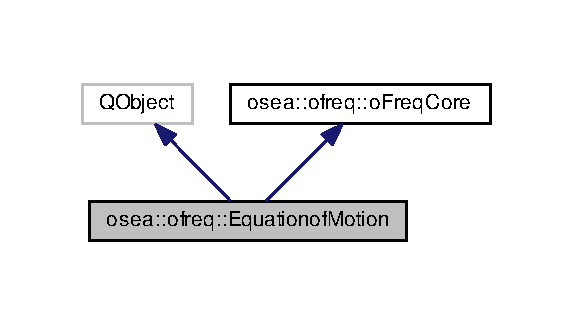
\includegraphics[height=550pt]{classosea_1_1ofreq_1_1_equationof_motion__inherit__graph}
\end{center}
\end{figure}
\subsection*{Public Member Functions}
\begin{DoxyCompactItemize}
\item 
\hyperlink{classosea_1_1ofreq_1_1_equationof_motion_a61c6e25419cf9c5402a4e30496ef6b19}{Equationof\-Motion} (\hyperlink{classosea_1_1ofreq_1_1_motion_model}{Motion\-Model} $\ast$model\-In)
\begin{DoxyCompactList}\small\item\em Default contrustor. Contains a reference to the motion model class which constructs it. \end{DoxyCompactList}\item 
\hyperlink{classosea_1_1ofreq_1_1_equationof_motion_adb22faa7fbb72f4ee01931fe6b9571ee}{Equationof\-Motion} (\hyperlink{classosea_1_1ofreq_1_1_motion_model}{Motion\-Model} $\ast$model\-In, std\-::string Name\-In)
\begin{DoxyCompactList}\small\item\em Contrustor with name. Contains a reference to the motion model class which constructs it. \end{DoxyCompactList}\item 
\hyperlink{classosea_1_1ofreq_1_1_equationof_motion_a334a999be59f6cba06cbbb2cf3134ad9}{Equationof\-Motion} (\hyperlink{classosea_1_1ofreq_1_1_motion_model}{Motion\-Model} $\ast$model\-In, std\-::string Name\-In, int Index\-In)
\begin{DoxyCompactList}\small\item\em Contrustor with name and index. Contains a reference to the motion model class which constructs it. \end{DoxyCompactList}\item 
virtual \hyperlink{classosea_1_1ofreq_1_1_equationof_motion_ab06097df1a54719d7a5682babbd9f233}{$\sim$\-Equationof\-Motion} ()
\begin{DoxyCompactList}\small\item\em Default destructor. \end{DoxyCompactList}\item 
virtual std\-::complex$<$ double $>$ \hyperlink{classosea_1_1ofreq_1_1_equationof_motion_a7198b4661f6c0a4c1f280863228bd63c}{Evaluate} ()
\begin{DoxyCompactList}\small\item\em Triggers evaluation of the equation of motion object. \end{DoxyCompactList}\item 
void \hyperlink{classosea_1_1ofreq_1_1_equationof_motion_a5a8674f3d8715973fa0affc162ae677c}{set\-Data\-Index} (int Data\-In)
\begin{DoxyCompactList}\small\item\em Sets the index for the equation of motion. \end{DoxyCompactList}\item 
int \hyperlink{classosea_1_1ofreq_1_1_equationof_motion_a45052d6a9814ffa899d1824f5d8e8cee}{get\-Data\-Index} ()
\begin{DoxyCompactList}\small\item\em Gets the index for the equation of motion. \end{DoxyCompactList}\item 
int \& \hyperlink{classosea_1_1ofreq_1_1_equationof_motion_ae16051cbf725210aa44941d41d8800e2}{ref\-Data\-Index} ()
\begin{DoxyCompactList}\small\item\em Gets the index for the equation of motion. \end{DoxyCompactList}\item 
void \hyperlink{classosea_1_1ofreq_1_1_equationof_motion_a154640d80a23348fa9183b6c4ebe3f37}{set\-Arguments} (int argn, std\-::vector$<$ double $>$ argv)
\begin{DoxyCompactList}\small\item\em Sets any values for arguments that may be used by the equation of motion. \end{DoxyCompactList}\item 
std\-::string \& \hyperlink{classosea_1_1ofreq_1_1_equationof_motion_abb7b1a4295e8406ea4f155b1f03689f6}{ref\-Name} ()
\begin{DoxyCompactList}\small\item\em The name for the equation object. \end{DoxyCompactList}\item 
void \hyperlink{classosea_1_1ofreq_1_1_equationof_motion_a1dba2d5b5a3d8c156c010ccb39c3bbe0}{set\-Name} (std\-::string name\-In)
\begin{DoxyCompactList}\small\item\em The name for the equation object. \end{DoxyCompactList}\item 
std\-::string \& \hyperlink{classosea_1_1ofreq_1_1_equationof_motion_a5be5a333dd1a5a65eaadec4b32c68fb5}{ref\-Description} ()
\begin{DoxyCompactList}\small\item\em The description for the equation object. \end{DoxyCompactList}\item 
void \hyperlink{classosea_1_1ofreq_1_1_equationof_motion_a307e0f8ada534f1fb17c06073101f8ab}{set\-Description} (std\-::string desc\-In)
\begin{DoxyCompactList}\small\item\em The description for the equation object. \end{DoxyCompactList}\item 
void \hyperlink{classosea_1_1ofreq_1_1_equationof_motion_a91bffb1d1129135369d6120033232b5c}{set\-Debug\-Data} (double freq\-In, std\-::complex$<$ double $>$ soln\-In, bool coeff\-In=false)
\begin{DoxyCompactList}\small\item\em Sets debugging data to use when creating fictional inputs purely for debugging this function. Allows the programmer to debug the function independent of the other functions which depend on it. \end{DoxyCompactList}\end{DoxyCompactItemize}
\subsection*{Protected Member Functions}
\begin{DoxyCompactItemize}
\item 
virtual std\-::complex$<$ double $>$ \hyperlink{classosea_1_1ofreq_1_1_equationof_motion_a1d8614b11de9396f3795e4b560e6c368}{set\-Formula} ()
\begin{DoxyCompactList}\small\item\em The formula used by the equation of motion. \end{DoxyCompactList}\item 
std\-::complex$<$ double $>$ \hyperlink{classosea_1_1ofreq_1_1_equationof_motion_ad4ba6707460a9db7f8103157af0cae65}{Kronecker} (int var1, int var2, bool anti=false)
\begin{DoxyCompactList}\small\item\em The mathematical Kronecker delta function. \end{DoxyCompactList}\item 
std\-::complex$<$ double $>$ \hyperlink{classosea_1_1ofreq_1_1_equationof_motion_af12570e012041ea91d81820735b14c74}{Ddt} (int \hyperlink{classosea_1_1ofreq_1_1_equationof_motion_ab69511cc5037376cf7da80ce30d9eaab}{var}, int \hyperlink{classosea_1_1ofreq_1_1_equationof_motion_a31f904818ce75c9e2a2b5cff9fc707a5}{ord}, int bod\-In=-\/1)
\begin{DoxyCompactList}\small\item\em Time differential function. \end{DoxyCompactList}\item 
std\-::complex$<$ double $>$ \hyperlink{classosea_1_1ofreq_1_1_equationof_motion_a61f33c3fd47ae2b66db1982b9c973ec1}{Force\-Active\-\_\-hydro} ()
\begin{DoxyCompactList}\small\item\em A reference to the data set of the Force\-Active\-\_\-hydro. \end{DoxyCompactList}\item 
std\-::complex$<$ double $>$ \hyperlink{classosea_1_1ofreq_1_1_equationof_motion_a238df115825cbe08522bdc10b84880b9}{Force\-Active\-\_\-user} ()
\begin{DoxyCompactList}\small\item\em A reference to the data set of the Force\-Active\-\_\-user. \end{DoxyCompactList}\item 
std\-::complex$<$ double $>$ \hyperlink{classosea_1_1ofreq_1_1_equationof_motion_a4962df48c786fced4e953e50f1d82a3a}{Force\-React\-\_\-hydro} (unsigned int ord\-In, unsigned int var\-In)
\begin{DoxyCompactList}\small\item\em A reference to the data set of the Force\-React\-\_\-hydro. \end{DoxyCompactList}\item 
std\-::complex$<$ double $>$ \hyperlink{classosea_1_1ofreq_1_1_equationof_motion_ac1f572e423c09b9e9fa955f52434a8f7}{Force\-React\-\_\-user} (unsigned int ord\-In, unsigned int var\-In)
\begin{DoxyCompactList}\small\item\em A reference to the data set of the Force\-React\-\_\-user. \end{DoxyCompactList}\item 
std\-::complex$<$ double $>$ \hyperlink{classosea_1_1ofreq_1_1_equationof_motion_af1d1f42b77561e9f1c4110e16af309da}{Force\-Cross\-\_\-hydro} (unsigned int bod\-In, unsigned int ord\-In, unsigned int var\-In)
\begin{DoxyCompactList}\small\item\em A reference to the data set of the Force\-Cross\-\_\-hydro. \end{DoxyCompactList}\item 
std\-::complex$<$ double $>$ \hyperlink{classosea_1_1ofreq_1_1_equationof_motion_a3b06b1ff4b792ad3a3d3c0274426d5ed}{Force\-Cross\-\_\-user} (unsigned int bod\-In, unsigned int ord\-In, unsigned int var\-In)
\begin{DoxyCompactList}\small\item\em A reference to the data set of the Force\-Cross\-\_\-user. \end{DoxyCompactList}\item 
std\-::complex$<$ double $>$ \hyperlink{classosea_1_1ofreq_1_1_equationof_motion_a848b45b70d29d793b86a7c1ca8f97ed6}{Force\-Mass} (int var\-In)
\begin{DoxyCompactList}\small\item\em A reference to the data set of the Force\-Mass. \end{DoxyCompactList}\item 
int \hyperlink{classosea_1_1ofreq_1_1_equationof_motion_ab69511cc5037376cf7da80ce30d9eaab}{var} ()
\begin{DoxyCompactList}\small\item\em Returns the index integer for iteration on variable. \end{DoxyCompactList}\item 
int \hyperlink{classosea_1_1ofreq_1_1_equationof_motion_a31f904818ce75c9e2a2b5cff9fc707a5}{ord} ()
\begin{DoxyCompactList}\small\item\em Returns the index integer for iteration on order of derviative. \end{DoxyCompactList}\item 
int \hyperlink{classosea_1_1ofreq_1_1_equationof_motion_ac87fe1d5112f5b42f9afd5f1c3b9002c}{body} ()
\begin{DoxyCompactList}\small\item\em Retuns the index integer for the body in the list of bodies. \end{DoxyCompactList}\item 
int \hyperlink{classosea_1_1ofreq_1_1_equationof_motion_a2fd7f9778dced5bba0d362841cf182a7}{curbody} ()
\begin{DoxyCompactList}\small\item\em Returns the index integer for the current body used by the motion model that created this equation of motion. \end{DoxyCompactList}\item 
std\-::complex$<$ double $>$ \hyperlink{classosea_1_1ofreq_1_1_equationof_motion_a5907d782ee639d5ec24515ed21050851}{Sum} (std\-::string Func\-Name, std\-::string index, int from=-\/1, int to=-\/1)
\begin{DoxyCompactList}\small\item\em Sums across a variable. \end{DoxyCompactList}\item 
std\-::complex$<$ double $>$ \hyperlink{classosea_1_1ofreq_1_1_equationof_motion_ab255de5deaef7394c788bb68a432aec0}{Sum} (std\-::complex$<$ double $>$($\ast$force)(void), int from, int to)
\begin{DoxyCompactList}\small\item\em Sums a function multiple times. \end{DoxyCompactList}\item 
std\-::complex$<$ double $>$ \hyperlink{classosea_1_1ofreq_1_1_equationof_motion_a44797e6d9ebed0de563ac08d15f8035f}{Sum} (std\-::complex$<$ double $>$ force, int from, int to)
\begin{DoxyCompactList}\small\item\em Sums a constant value multiple times. \end{DoxyCompactList}\item 
virtual std\-::complex$<$ double $>$ \hyperlink{classosea_1_1ofreq_1_1_equationof_motion_af83fcd0f9089a49f0b36e1af79b66922}{Func1} ()
\begin{DoxyCompactList}\small\item\em Func1 through Func50 provide user custom defined functions. \end{DoxyCompactList}\item 
virtual std\-::complex$<$ double $>$ \hyperlink{classosea_1_1ofreq_1_1_equationof_motion_accd87271595a2eac0dc116285479ecff}{Func2} ()
\item 
virtual std\-::complex$<$ double $>$ \hyperlink{classosea_1_1ofreq_1_1_equationof_motion_ad63157443d3a7b67ec961a8642f895e4}{Func3} ()
\item 
virtual std\-::complex$<$ double $>$ \hyperlink{classosea_1_1ofreq_1_1_equationof_motion_a6e604ceb9f5147327d51099ca9cc862b}{Func4} ()
\item 
virtual std\-::complex$<$ double $>$ \hyperlink{classosea_1_1ofreq_1_1_equationof_motion_af8950ca2b293588b39b169bc18f6864d}{Func5} ()
\item 
virtual std\-::complex$<$ double $>$ \hyperlink{classosea_1_1ofreq_1_1_equationof_motion_aecb9d2662b2fc77143649ebbeaddb5af}{Func6} ()
\item 
virtual std\-::complex$<$ double $>$ \hyperlink{classosea_1_1ofreq_1_1_equationof_motion_a99c266e01afc3f20b7154db38344a050}{Func7} ()
\item 
virtual std\-::complex$<$ double $>$ \hyperlink{classosea_1_1ofreq_1_1_equationof_motion_a20b071061e22794f809e8e4a711385a9}{Func8} ()
\item 
virtual std\-::complex$<$ double $>$ \hyperlink{classosea_1_1ofreq_1_1_equationof_motion_aa5544ff6b4afe0982124ba173392cde6}{Func9} ()
\item 
virtual std\-::complex$<$ double $>$ \hyperlink{classosea_1_1ofreq_1_1_equationof_motion_a9d087d68b0af5a5c923cf624ba2ca25d}{Func10} ()
\item 
virtual std\-::complex$<$ double $>$ \hyperlink{classosea_1_1ofreq_1_1_equationof_motion_a93650f458441e585dbe6bae34934a5ca}{Func11} ()
\item 
virtual std\-::complex$<$ double $>$ \hyperlink{classosea_1_1ofreq_1_1_equationof_motion_a73499ca765a883d14483f0894cb99d6b}{Func12} ()
\item 
virtual std\-::complex$<$ double $>$ \hyperlink{classosea_1_1ofreq_1_1_equationof_motion_ab0a6e7f35c1ee774c67c348f63218161}{Func13} ()
\item 
virtual std\-::complex$<$ double $>$ \hyperlink{classosea_1_1ofreq_1_1_equationof_motion_a95dd987ce8564fc96f3c4dfd1b00da72}{Func14} ()
\item 
virtual std\-::complex$<$ double $>$ \hyperlink{classosea_1_1ofreq_1_1_equationof_motion_a6fb116fda50fff5f6a551033809866bc}{Func15} ()
\item 
virtual std\-::complex$<$ double $>$ \hyperlink{classosea_1_1ofreq_1_1_equationof_motion_aad2958f7e57f06d5b7a9f807d565bbc7}{Func16} ()
\item 
virtual std\-::complex$<$ double $>$ \hyperlink{classosea_1_1ofreq_1_1_equationof_motion_a9b2c9a471dbc0d48ddf025a8a0c55f1f}{Func17} ()
\item 
virtual std\-::complex$<$ double $>$ \hyperlink{classosea_1_1ofreq_1_1_equationof_motion_a3cbd356ecdd5bc045dc98421d6283170}{Func18} ()
\item 
virtual std\-::complex$<$ double $>$ \hyperlink{classosea_1_1ofreq_1_1_equationof_motion_a27e79b31834844a40c870436ac62ae73}{Func19} ()
\item 
virtual std\-::complex$<$ double $>$ \hyperlink{classosea_1_1ofreq_1_1_equationof_motion_a7232042c946e1e2fd2c5d6e9e5929300}{Func20} ()
\item 
virtual std\-::complex$<$ double $>$ \hyperlink{classosea_1_1ofreq_1_1_equationof_motion_a771493c65f06e5085e3b0c9150aa0427}{Func21} ()
\item 
virtual std\-::complex$<$ double $>$ \hyperlink{classosea_1_1ofreq_1_1_equationof_motion_aa9924875622062551456bab5ea3ecb20}{Func22} ()
\item 
virtual std\-::complex$<$ double $>$ \hyperlink{classosea_1_1ofreq_1_1_equationof_motion_ac5cf42463f4da9f251436e80da15499a}{Func23} ()
\item 
virtual std\-::complex$<$ double $>$ \hyperlink{classosea_1_1ofreq_1_1_equationof_motion_abe255c1e5217273f9adfc3c4c5f83727}{Func24} ()
\item 
virtual std\-::complex$<$ double $>$ \hyperlink{classosea_1_1ofreq_1_1_equationof_motion_a22e70f9d370ce2bd8d10621d6b686da8}{Func25} ()
\item 
virtual std\-::complex$<$ double $>$ \hyperlink{classosea_1_1ofreq_1_1_equationof_motion_aef40214a54959ffffd9b4c45e3fa0648}{Func26} ()
\item 
virtual std\-::complex$<$ double $>$ \hyperlink{classosea_1_1ofreq_1_1_equationof_motion_af534561eec5a3d27212076a60043a23c}{Func27} ()
\item 
virtual std\-::complex$<$ double $>$ \hyperlink{classosea_1_1ofreq_1_1_equationof_motion_a6d12f67c42964bef80db4268b8033c6d}{Func28} ()
\item 
virtual std\-::complex$<$ double $>$ \hyperlink{classosea_1_1ofreq_1_1_equationof_motion_a9e62ab3a3096c28a578367332d5846da}{Func29} ()
\item 
virtual std\-::complex$<$ double $>$ \hyperlink{classosea_1_1ofreq_1_1_equationof_motion_a172d2920a71a1b24f467994f6fea8f99}{Func30} ()
\item 
virtual std\-::complex$<$ double $>$ \hyperlink{classosea_1_1ofreq_1_1_equationof_motion_a5b020264aabe3cdaf95c04e9e7ca1874}{Func31} ()
\item 
virtual std\-::complex$<$ double $>$ \hyperlink{classosea_1_1ofreq_1_1_equationof_motion_a240b245630cd6751721233de8560200a}{Func32} ()
\item 
virtual std\-::complex$<$ double $>$ \hyperlink{classosea_1_1ofreq_1_1_equationof_motion_a9f12298af512bf091c3b8a57c1e5f96c}{Func33} ()
\item 
virtual std\-::complex$<$ double $>$ \hyperlink{classosea_1_1ofreq_1_1_equationof_motion_aa162c47e961c0e3064bd0d57e5c60764}{Func34} ()
\item 
virtual std\-::complex$<$ double $>$ \hyperlink{classosea_1_1ofreq_1_1_equationof_motion_ac658169efe42c44bb5e14c5f9131478c}{Func35} ()
\item 
virtual std\-::complex$<$ double $>$ \hyperlink{classosea_1_1ofreq_1_1_equationof_motion_a51a0d7c4447833b5d26cf3624623bd33}{Func36} ()
\item 
virtual std\-::complex$<$ double $>$ \hyperlink{classosea_1_1ofreq_1_1_equationof_motion_a80f3f61eaded9b475fbb47aaf335183f}{Func37} ()
\item 
virtual std\-::complex$<$ double $>$ \hyperlink{classosea_1_1ofreq_1_1_equationof_motion_a01727a601ff0281f16591ef4d1b5bbf0}{Func38} ()
\item 
virtual std\-::complex$<$ double $>$ \hyperlink{classosea_1_1ofreq_1_1_equationof_motion_a5e986c0952ec3c25426bba62737633f1}{Func39} ()
\item 
virtual std\-::complex$<$ double $>$ \hyperlink{classosea_1_1ofreq_1_1_equationof_motion_aeefb90327b72c61c09a22d2bed6ebd60}{Func40} ()
\item 
virtual std\-::complex$<$ double $>$ \hyperlink{classosea_1_1ofreq_1_1_equationof_motion_af6ac5c3c8cfd7ae351693bb349d6f28a}{Func41} ()
\item 
virtual std\-::complex$<$ double $>$ \hyperlink{classosea_1_1ofreq_1_1_equationof_motion_a8a7b456c14cbbf5a284bc6438eedaec9}{Func42} ()
\item 
virtual std\-::complex$<$ double $>$ \hyperlink{classosea_1_1ofreq_1_1_equationof_motion_a9b70e7f90d34a774a4a19b77b759a7d5}{Func43} ()
\item 
virtual std\-::complex$<$ double $>$ \hyperlink{classosea_1_1ofreq_1_1_equationof_motion_aa85ed6fe8cee4a23ed82947b32aa8afd}{Func44} ()
\item 
virtual std\-::complex$<$ double $>$ \hyperlink{classosea_1_1ofreq_1_1_equationof_motion_af447cb3b12a7dd0667a2e1ebf95b9012}{Func45} ()
\item 
virtual std\-::complex$<$ double $>$ \hyperlink{classosea_1_1ofreq_1_1_equationof_motion_ae26b7d1ec3c7ac4d8e16188e46cc3350}{Func46} ()
\item 
virtual std\-::complex$<$ double $>$ \hyperlink{classosea_1_1ofreq_1_1_equationof_motion_a63049815de6897a3e981939434e2435c}{Func47} ()
\item 
virtual std\-::complex$<$ double $>$ \hyperlink{classosea_1_1ofreq_1_1_equationof_motion_ae6eb5b8e68ea3ea44cecc4a528e61d1c}{Func48} ()
\item 
virtual std\-::complex$<$ double $>$ \hyperlink{classosea_1_1ofreq_1_1_equationof_motion_af5fc7d0ef4f09f546779bbab205603e8}{Func49} ()
\item 
virtual std\-::complex$<$ double $>$ \hyperlink{classosea_1_1ofreq_1_1_equationof_motion_acb2bacacd96cf28600678e1a5a0ae397}{Func50} ()
\end{DoxyCompactItemize}
\subsection*{Protected Attributes}
\begin{DoxyCompactItemize}
\item 
int \hyperlink{classosea_1_1ofreq_1_1_equationof_motion_a13a15811fd575ac0fccf0d463218657b}{argcount}
\begin{DoxyCompactList}\small\item\em Used to supply arguments to the equation of motion. Recods the number of arguments. \end{DoxyCompactList}\item 
std\-::vector$<$ double $>$ \hyperlink{classosea_1_1ofreq_1_1_equationof_motion_a1a9bf7f3460368c102aa8d4edec9b500}{argvalue}
\begin{DoxyCompactList}\small\item\em Used to supply arguments to the equation of motion. Uknown, arbitrary double precision values. A vector of uknown size. \end{DoxyCompactList}\item 
std\-::string \hyperlink{classosea_1_1ofreq_1_1_equationof_motion_a5848a1ad14d31556fd1b62b4e3de3643}{p\-Name}
\begin{DoxyCompactList}\small\item\em The name for the equation object. \end{DoxyCompactList}\item 
std\-::string \hyperlink{classosea_1_1ofreq_1_1_equationof_motion_aa6ce10dacd47441d445a9170bd355792}{p\-Description}
\begin{DoxyCompactList}\small\item\em The description for the equation object. \end{DoxyCompactList}\item 
unsigned int \hyperlink{classosea_1_1ofreq_1_1_equationof_motion_a88a53c5688c07a1cb90cdf5755782fcf}{p\-Cur\-Var}
\begin{DoxyCompactList}\small\item\em The integer of the current value of \hyperlink{classosea_1_1ofreq_1_1_equationof_motion_ab69511cc5037376cf7da80ce30d9eaab}{var()} index. Used for iteration and summation functions. \end{DoxyCompactList}\item 
unsigned int \hyperlink{classosea_1_1ofreq_1_1_equationof_motion_a39d41e27dcf84f163ef794a9287a0ef1}{p\-Cur\-Ord}
\begin{DoxyCompactList}\small\item\em The integer of the current value of \hyperlink{classosea_1_1ofreq_1_1_equationof_motion_a31f904818ce75c9e2a2b5cff9fc707a5}{ord()} index. Used for iteration and summation functions. \end{DoxyCompactList}\item 
unsigned int \hyperlink{classosea_1_1ofreq_1_1_equationof_motion_a5a1c11c4c4a827494a7772af0d0dddc6}{p\-Bod}
\begin{DoxyCompactList}\small\item\em The integer of the current body. Used for iteration and summation functions. \end{DoxyCompactList}\end{DoxyCompactItemize}
\subsection*{Static Protected Attributes}
\begin{DoxyCompactItemize}
\item 
static int \hyperlink{classosea_1_1ofreq_1_1_equationof_motion_ad00063eabf1b5075b04c6d2507acebd4}{undef\-Arg} = -\/1
\end{DoxyCompactItemize}
\subsection*{Additional Inherited Members}


\subsection{Detailed Description}
The \hyperlink{classosea_1_1ofreq_1_1_equation}{Equation} of motion class defines a single equation of motion. Each object of the class represents a new instance. This is the base class, which gets inheritted by any custom class. The only major definition added to any inherrited class is the actual formula definition for the equation. It may be that the equation are repetitions of the same sequence, just with a different equation index. In that case, multiple instances of the same class can be created and the equation index changed. This can save on typing. Or, if the equations are truly different for each equation, you can create a separate equation of motion class for each equation, and initiate with just one object from each class.

In addition to the regular object entries, the class also has provision for a list of arbitrary arguments. 

Definition at line 101 of file equationofmotion.\-h.



\subsection{Constructor \& Destructor Documentation}
\hypertarget{classosea_1_1ofreq_1_1_equationof_motion_a61c6e25419cf9c5402a4e30496ef6b19}{\index{osea\-::ofreq\-::\-Equationof\-Motion@{osea\-::ofreq\-::\-Equationof\-Motion}!Equationof\-Motion@{Equationof\-Motion}}
\index{Equationof\-Motion@{Equationof\-Motion}!osea::ofreq::EquationofMotion@{osea\-::ofreq\-::\-Equationof\-Motion}}
\subsubsection[{Equationof\-Motion}]{\setlength{\rightskip}{0pt plus 5cm}Equationof\-Motion\-::\-Equationof\-Motion (
\begin{DoxyParamCaption}
\item[{{\bf Motion\-Model} $\ast$}]{model\-In}
\end{DoxyParamCaption}
)}}\label{classosea_1_1ofreq_1_1_equationof_motion_a61c6e25419cf9c5402a4e30496ef6b19}


Default contrustor. Contains a reference to the motion model class which constructs it. 

Default contrustor. Contains a reference to the motion model class which constructs it. The constructing class is necessary because several functions in the Equation\-Of\-Motion class use data in the constructing class, the motion model class. 
\begin{DoxyParams}{Parameters}
{\em model\-In} & A pointer to the motion model object that created the equation of motion. \\
\hline
\end{DoxyParams}


Definition at line 46 of file equationofmotion.\-cpp.

\hypertarget{classosea_1_1ofreq_1_1_equationof_motion_adb22faa7fbb72f4ee01931fe6b9571ee}{\index{osea\-::ofreq\-::\-Equationof\-Motion@{osea\-::ofreq\-::\-Equationof\-Motion}!Equationof\-Motion@{Equationof\-Motion}}
\index{Equationof\-Motion@{Equationof\-Motion}!osea::ofreq::EquationofMotion@{osea\-::ofreq\-::\-Equationof\-Motion}}
\subsubsection[{Equationof\-Motion}]{\setlength{\rightskip}{0pt plus 5cm}osea\-::ofreq\-::\-Equationof\-Motion\-::\-Equationof\-Motion (
\begin{DoxyParamCaption}
\item[{{\bf Motion\-Model} $\ast$}]{model\-In, }
\item[{std\-::string}]{Name\-In}
\end{DoxyParamCaption}
)}}\label{classosea_1_1ofreq_1_1_equationof_motion_adb22faa7fbb72f4ee01931fe6b9571ee}


Contrustor with name. Contains a reference to the motion model class which constructs it. 

Default contrustor. Contains a reference to the motion model class which constructs it. The constructing class is necessary because several functions in the Equation\-Of\-Motion class use data in the constructing class, the motion model class. 
\begin{DoxyParams}{Parameters}
{\em model\-In} & A pointer to the motion model object that created the equation of motion. \\
\hline
{\em Name\-In} & A name for what physical property the equation solves for. Used for user output. Not critical to program execution. \\
\hline
\end{DoxyParams}
\hypertarget{classosea_1_1ofreq_1_1_equationof_motion_a334a999be59f6cba06cbbb2cf3134ad9}{\index{osea\-::ofreq\-::\-Equationof\-Motion@{osea\-::ofreq\-::\-Equationof\-Motion}!Equationof\-Motion@{Equationof\-Motion}}
\index{Equationof\-Motion@{Equationof\-Motion}!osea::ofreq::EquationofMotion@{osea\-::ofreq\-::\-Equationof\-Motion}}
\subsubsection[{Equationof\-Motion}]{\setlength{\rightskip}{0pt plus 5cm}osea\-::ofreq\-::\-Equationof\-Motion\-::\-Equationof\-Motion (
\begin{DoxyParamCaption}
\item[{{\bf Motion\-Model} $\ast$}]{model\-In, }
\item[{std\-::string}]{Name\-In, }
\item[{int}]{Index\-In}
\end{DoxyParamCaption}
)}}\label{classosea_1_1ofreq_1_1_equationof_motion_a334a999be59f6cba06cbbb2cf3134ad9}


Contrustor with name and index. Contains a reference to the motion model class which constructs it. 

Default contrustor. Contains a reference to the motion model class which constructs it. The constructing class is necessary because several functions in the Equation\-Of\-Motion class use data in the constructing class, the motion model class. 
\begin{DoxyParams}{Parameters}
{\em model\-In} & A pointer to the motion model object that created the equation of motion. \\
\hline
{\em Name\-In} & A name for what physical property the equation solves for. Used for user output. Not critical to program execution. \\
\hline
{\em Index\-In} & Sets the index for the \hyperlink{classosea_1_1ofreq_1_1_equation}{Equation} of Motion. The index is how the equation determines which numbers to access on the data. The following indices are used. Any higher indices can extend beyond this range, and the program easily adapts. But the following three are reserved. Unused indices are not transferred to the matrices when solved. So unused indices to not negatively impact calculation performance. However, using excessively large indices (say 500 when you only have 3 equations) will result in large matrices and unecessary memory requirements. T\-He following index reservations apply. 1\-: Translation in x-\/direction. Specific to rigid body motion. 2\-: Translation in y-\/direction. Specific to rigid body motion. 3\-: Translation in z-\/direction. Specific to rigid body motion. 4\-: Rotation about x-\/direction. Specific to rigid body motion. 5\-: Rotation about y-\/direction. Specific to rigid body motion. 6\-: Rotation about z-\/direction. Specific to rigid body motion. \\
\hline
\end{DoxyParams}
\hypertarget{classosea_1_1ofreq_1_1_equationof_motion_ab06097df1a54719d7a5682babbd9f233}{\index{osea\-::ofreq\-::\-Equationof\-Motion@{osea\-::ofreq\-::\-Equationof\-Motion}!$\sim$\-Equationof\-Motion@{$\sim$\-Equationof\-Motion}}
\index{$\sim$\-Equationof\-Motion@{$\sim$\-Equationof\-Motion}!osea::ofreq::EquationofMotion@{osea\-::ofreq\-::\-Equationof\-Motion}}
\subsubsection[{$\sim$\-Equationof\-Motion}]{\setlength{\rightskip}{0pt plus 5cm}Equationof\-Motion\-::$\sim$\-Equationof\-Motion (
\begin{DoxyParamCaption}
{}
\end{DoxyParamCaption}
)\hspace{0.3cm}{\ttfamily [virtual]}}}\label{classosea_1_1ofreq_1_1_equationof_motion_ab06097df1a54719d7a5682babbd9f233}


Default destructor. 



Definition at line 81 of file equationofmotion.\-cpp.



\subsection{Member Function Documentation}
\hypertarget{classosea_1_1ofreq_1_1_equationof_motion_ac87fe1d5112f5b42f9afd5f1c3b9002c}{\index{osea\-::ofreq\-::\-Equationof\-Motion@{osea\-::ofreq\-::\-Equationof\-Motion}!body@{body}}
\index{body@{body}!osea::ofreq::EquationofMotion@{osea\-::ofreq\-::\-Equationof\-Motion}}
\subsubsection[{body}]{\setlength{\rightskip}{0pt plus 5cm}int Equationof\-Motion\-::body (
\begin{DoxyParamCaption}
{}
\end{DoxyParamCaption}
)\hspace{0.3cm}{\ttfamily [protected]}}}\label{classosea_1_1ofreq_1_1_equationof_motion_ac87fe1d5112f5b42f9afd5f1c3b9002c}


Retuns the index integer for the body in the list of bodies. 

This is used for summation functions when iterating through each body in the list of bodies. This index cannot be modified through this function. It is purely meant for access to the variable. \begin{DoxyReturn}{Returns}
Returns the index integer for each body in the list of bodies. 
\end{DoxyReturn}


Definition at line 717 of file equationofmotion.\-cpp.

\hypertarget{classosea_1_1ofreq_1_1_equationof_motion_a2fd7f9778dced5bba0d362841cf182a7}{\index{osea\-::ofreq\-::\-Equationof\-Motion@{osea\-::ofreq\-::\-Equationof\-Motion}!curbody@{curbody}}
\index{curbody@{curbody}!osea::ofreq::EquationofMotion@{osea\-::ofreq\-::\-Equationof\-Motion}}
\subsubsection[{curbody}]{\setlength{\rightskip}{0pt plus 5cm}int Equationof\-Motion\-::curbody (
\begin{DoxyParamCaption}
{}
\end{DoxyParamCaption}
)\hspace{0.3cm}{\ttfamily [protected]}}}\label{classosea_1_1ofreq_1_1_equationof_motion_a2fd7f9778dced5bba0d362841cf182a7}


Returns the index integer for the current body used by the motion model that created this equation of motion. 

This index cannot be modified through this function. It is purely meant for access of the variable. \begin{DoxyReturn}{Returns}
Returns the index integer for the current body used by the motion model that created this equation of motions. 
\end{DoxyReturn}


Definition at line 724 of file equationofmotion.\-cpp.

\hypertarget{classosea_1_1ofreq_1_1_equationof_motion_af12570e012041ea91d81820735b14c74}{\index{osea\-::ofreq\-::\-Equationof\-Motion@{osea\-::ofreq\-::\-Equationof\-Motion}!Ddt@{Ddt}}
\index{Ddt@{Ddt}!osea::ofreq::EquationofMotion@{osea\-::ofreq\-::\-Equationof\-Motion}}
\subsubsection[{Ddt}]{\setlength{\rightskip}{0pt plus 5cm}complex$<$ double $>$ Equationof\-Motion\-::\-Ddt (
\begin{DoxyParamCaption}
\item[{int}]{var, }
\item[{int}]{ord, }
\item[{int}]{bod\-In = {\ttfamily -\/1}}
\end{DoxyParamCaption}
)\hspace{0.3cm}{\ttfamily [protected]}}}\label{classosea_1_1ofreq_1_1_equationof_motion_af12570e012041ea91d81820735b14c74}


Time differential function. 

Time differential function. Used to calculate the time derivative of a reponse. Can convert from response amplitude to velocity to acceleration, and further. Used to calculated amplitude of response. 
\begin{DoxyParams}{Parameters}
{\em var} & Index of the variable to use for the time differential. If included with the function \hyperlink{classosea_1_1ofreq_1_1_equationof_motion_ab69511cc5037376cf7da80ce30d9eaab}{var()}, the index is automatically determined by the summation functions that you include \hyperlink{classosea_1_1ofreq_1_1_equationof_motion_af12570e012041ea91d81820735b14c74}{Ddt()} into. \\
\hline
{\em ord} & Integer. The order of the differential. If the function \hyperlink{classosea_1_1ofreq_1_1_equationof_motion_a31f904818ce75c9e2a2b5cff9fc707a5}{ord()} is used, the order is automatically determined by the summation function that you include \hyperlink{classosea_1_1ofreq_1_1_equationof_motion_af12570e012041ea91d81820735b14c74}{Ddt()} into. \\
\hline
{\em bod\-In} & The body to retrieve variable data for. \\
\hline
\end{DoxyParams}
\begin{DoxyReturn}{Returns}
Returns a complex value that is the time differential, transposed into a frequency domain. If absolute values of response were desired, the function will include the effects of response amplitude. 
\end{DoxyReturn}


Definition at line 219 of file equationofmotion.\-cpp.

\hypertarget{classosea_1_1ofreq_1_1_equationof_motion_a7198b4661f6c0a4c1f280863228bd63c}{\index{osea\-::ofreq\-::\-Equationof\-Motion@{osea\-::ofreq\-::\-Equationof\-Motion}!Evaluate@{Evaluate}}
\index{Evaluate@{Evaluate}!osea::ofreq::EquationofMotion@{osea\-::ofreq\-::\-Equationof\-Motion}}
\subsubsection[{Evaluate}]{\setlength{\rightskip}{0pt plus 5cm}complex$<$ double $>$ Equationof\-Motion\-::\-Evaluate (
\begin{DoxyParamCaption}
{}
\end{DoxyParamCaption}
)\hspace{0.3cm}{\ttfamily [virtual]}}}\label{classosea_1_1ofreq_1_1_equationof_motion_a7198b4661f6c0a4c1f280863228bd63c}


Triggers evaluation of the equation of motion object. 

\begin{DoxyReturn}{Returns}
Returns a complex number that is the result of evaluating the equation of motion object. 
\end{DoxyReturn}


Definition at line 87 of file equationofmotion.\-cpp.

\hypertarget{classosea_1_1ofreq_1_1_equationof_motion_a61f33c3fd47ae2b66db1982b9c973ec1}{\index{osea\-::ofreq\-::\-Equationof\-Motion@{osea\-::ofreq\-::\-Equationof\-Motion}!Force\-Active\-\_\-hydro@{Force\-Active\-\_\-hydro}}
\index{Force\-Active\-\_\-hydro@{Force\-Active\-\_\-hydro}!osea::ofreq::EquationofMotion@{osea\-::ofreq\-::\-Equationof\-Motion}}
\subsubsection[{Force\-Active\-\_\-hydro}]{\setlength{\rightskip}{0pt plus 5cm}complex$<$ double $>$ Equationof\-Motion\-::\-Force\-Active\-\_\-hydro (
\begin{DoxyParamCaption}
{}
\end{DoxyParamCaption}
)\hspace{0.3cm}{\ttfamily [protected]}}}\label{classosea_1_1ofreq_1_1_equationof_motion_a61f33c3fd47ae2b66db1982b9c973ec1}


A reference to the data set of the Force\-Active\-\_\-hydro. 

\begin{DoxyReturn}{Returns}
Returns the data set for the Force\-Active\-\_\-hydro. Indices can be specified to access individual elements. 
\end{DoxyReturn}


Definition at line 282 of file equationofmotion.\-cpp.

\hypertarget{classosea_1_1ofreq_1_1_equationof_motion_a238df115825cbe08522bdc10b84880b9}{\index{osea\-::ofreq\-::\-Equationof\-Motion@{osea\-::ofreq\-::\-Equationof\-Motion}!Force\-Active\-\_\-user@{Force\-Active\-\_\-user}}
\index{Force\-Active\-\_\-user@{Force\-Active\-\_\-user}!osea::ofreq::EquationofMotion@{osea\-::ofreq\-::\-Equationof\-Motion}}
\subsubsection[{Force\-Active\-\_\-user}]{\setlength{\rightskip}{0pt plus 5cm}complex$<$ double $>$ Equationof\-Motion\-::\-Force\-Active\-\_\-user (
\begin{DoxyParamCaption}
{}
\end{DoxyParamCaption}
)\hspace{0.3cm}{\ttfamily [protected]}}}\label{classosea_1_1ofreq_1_1_equationof_motion_a238df115825cbe08522bdc10b84880b9}


A reference to the data set of the Force\-Active\-\_\-user. 

\begin{DoxyReturn}{Returns}
Returns the data set for the Force\-Active\-\_\-user. Indices can be specified to access individual elements. 
\end{DoxyReturn}


Definition at line 328 of file equationofmotion.\-cpp.

\hypertarget{classosea_1_1ofreq_1_1_equationof_motion_af1d1f42b77561e9f1c4110e16af309da}{\index{osea\-::ofreq\-::\-Equationof\-Motion@{osea\-::ofreq\-::\-Equationof\-Motion}!Force\-Cross\-\_\-hydro@{Force\-Cross\-\_\-hydro}}
\index{Force\-Cross\-\_\-hydro@{Force\-Cross\-\_\-hydro}!osea::ofreq::EquationofMotion@{osea\-::ofreq\-::\-Equationof\-Motion}}
\subsubsection[{Force\-Cross\-\_\-hydro}]{\setlength{\rightskip}{0pt plus 5cm}complex$<$ double $>$ Equationof\-Motion\-::\-Force\-Cross\-\_\-hydro (
\begin{DoxyParamCaption}
\item[{unsigned int}]{bod\-In, }
\item[{unsigned int}]{ord\-In, }
\item[{unsigned int}]{var\-In}
\end{DoxyParamCaption}
)\hspace{0.3cm}{\ttfamily [protected]}}}\label{classosea_1_1ofreq_1_1_equationof_motion_af1d1f42b77561e9f1c4110e16af309da}


A reference to the data set of the Force\-Cross\-\_\-hydro. 


\begin{DoxyParams}{Parameters}
{\em bod\-In} & Integer. Represents the input variable for the body that the cross body force is linked to. \\
\hline
{\em ord\-In} & Integer. Represents the input variable for the order of derivative. \\
\hline
{\em var\-In} & Integer. Represents the input varaible for the variable. \\
\hline
\end{DoxyParams}
\begin{DoxyReturn}{Returns}
Returns the data set for the Force\-Cross\-\_\-hydro. Indices can be specified to access individual elements. 
\end{DoxyReturn}


Definition at line 492 of file equationofmotion.\-cpp.

\hypertarget{classosea_1_1ofreq_1_1_equationof_motion_a3b06b1ff4b792ad3a3d3c0274426d5ed}{\index{osea\-::ofreq\-::\-Equationof\-Motion@{osea\-::ofreq\-::\-Equationof\-Motion}!Force\-Cross\-\_\-user@{Force\-Cross\-\_\-user}}
\index{Force\-Cross\-\_\-user@{Force\-Cross\-\_\-user}!osea::ofreq::EquationofMotion@{osea\-::ofreq\-::\-Equationof\-Motion}}
\subsubsection[{Force\-Cross\-\_\-user}]{\setlength{\rightskip}{0pt plus 5cm}complex$<$ double $>$ Equationof\-Motion\-::\-Force\-Cross\-\_\-user (
\begin{DoxyParamCaption}
\item[{unsigned int}]{bod\-In, }
\item[{unsigned int}]{ord\-In, }
\item[{unsigned int}]{var\-In}
\end{DoxyParamCaption}
)\hspace{0.3cm}{\ttfamily [protected]}}}\label{classosea_1_1ofreq_1_1_equationof_motion_a3b06b1ff4b792ad3a3d3c0274426d5ed}


A reference to the data set of the Force\-Cross\-\_\-user. 


\begin{DoxyParams}{Parameters}
{\em bod\-In} & Integer. Represents the input variable for the body that the cross body force is linked to. \\
\hline
{\em ord\-In} & Integer. Represents the input variable for the order of derivative. \\
\hline
{\em var\-In} & Integer. Represents the input varaible for the variable. \\
\hline
\end{DoxyParams}
\begin{DoxyReturn}{Returns}
Returns the data set for the Force\-Cross\-\_\-user. Indices can be specified to access individual elements. 
\end{DoxyReturn}


Definition at line 556 of file equationofmotion.\-cpp.

\hypertarget{classosea_1_1ofreq_1_1_equationof_motion_a848b45b70d29d793b86a7c1ca8f97ed6}{\index{osea\-::ofreq\-::\-Equationof\-Motion@{osea\-::ofreq\-::\-Equationof\-Motion}!Force\-Mass@{Force\-Mass}}
\index{Force\-Mass@{Force\-Mass}!osea::ofreq::EquationofMotion@{osea\-::ofreq\-::\-Equationof\-Motion}}
\subsubsection[{Force\-Mass}]{\setlength{\rightskip}{0pt plus 5cm}complex$<$ double $>$ Equationof\-Motion\-::\-Force\-Mass (
\begin{DoxyParamCaption}
\item[{int}]{var\-In}
\end{DoxyParamCaption}
)\hspace{0.3cm}{\ttfamily [protected]}}}\label{classosea_1_1ofreq_1_1_equationof_motion_a848b45b70d29d793b86a7c1ca8f97ed6}


A reference to the data set of the Force\-Mass. 


\begin{DoxyParams}{Parameters}
{\em var\-In} & Integer. Represents the input index for the variable. \\
\hline
\end{DoxyParams}
\begin{DoxyReturn}{Returns}
Returns the data set for the Force\-Mass. Indices can be specified to access individual elements. 
\end{DoxyReturn}


Definition at line 619 of file equationofmotion.\-cpp.

\hypertarget{classosea_1_1ofreq_1_1_equationof_motion_a4962df48c786fced4e953e50f1d82a3a}{\index{osea\-::ofreq\-::\-Equationof\-Motion@{osea\-::ofreq\-::\-Equationof\-Motion}!Force\-React\-\_\-hydro@{Force\-React\-\_\-hydro}}
\index{Force\-React\-\_\-hydro@{Force\-React\-\_\-hydro}!osea::ofreq::EquationofMotion@{osea\-::ofreq\-::\-Equationof\-Motion}}
\subsubsection[{Force\-React\-\_\-hydro}]{\setlength{\rightskip}{0pt plus 5cm}complex$<$ double $>$ Equationof\-Motion\-::\-Force\-React\-\_\-hydro (
\begin{DoxyParamCaption}
\item[{unsigned int}]{ord\-In, }
\item[{unsigned int}]{var\-In}
\end{DoxyParamCaption}
)\hspace{0.3cm}{\ttfamily [protected]}}}\label{classosea_1_1ofreq_1_1_equationof_motion_a4962df48c786fced4e953e50f1d82a3a}


A reference to the data set of the Force\-React\-\_\-hydro. 


\begin{DoxyParams}{Parameters}
{\em ord\-In} & Integer. Represents the input variable for the order of derivative. \\
\hline
{\em var\-In} & Integer. Represents the input varaible for the variable. \\
\hline
\end{DoxyParams}
\begin{DoxyReturn}{Returns}
Returns the data set for the Force\-React\-\_\-hydro. Indices can be specified to access individual elements. 
\end{DoxyReturn}


Definition at line 378 of file equationofmotion.\-cpp.

\hypertarget{classosea_1_1ofreq_1_1_equationof_motion_ac1f572e423c09b9e9fa955f52434a8f7}{\index{osea\-::ofreq\-::\-Equationof\-Motion@{osea\-::ofreq\-::\-Equationof\-Motion}!Force\-React\-\_\-user@{Force\-React\-\_\-user}}
\index{Force\-React\-\_\-user@{Force\-React\-\_\-user}!osea::ofreq::EquationofMotion@{osea\-::ofreq\-::\-Equationof\-Motion}}
\subsubsection[{Force\-React\-\_\-user}]{\setlength{\rightskip}{0pt plus 5cm}complex$<$ double $>$ Equationof\-Motion\-::\-Force\-React\-\_\-user (
\begin{DoxyParamCaption}
\item[{unsigned int}]{ord\-In, }
\item[{unsigned int}]{var\-In}
\end{DoxyParamCaption}
)\hspace{0.3cm}{\ttfamily [protected]}}}\label{classosea_1_1ofreq_1_1_equationof_motion_ac1f572e423c09b9e9fa955f52434a8f7}


A reference to the data set of the Force\-React\-\_\-user. 


\begin{DoxyParams}{Parameters}
{\em ord\-In} & Integer. Represents the input variable for the order of derivative. \\
\hline
{\em var\-In} & Integer. Represents the input varaible for the variable. \\
\hline
\end{DoxyParams}
\begin{DoxyReturn}{Returns}
Returns the data set for the Force\-React\-\_\-user. Indices can be specified to access individual elements. 
\end{DoxyReturn}


Definition at line 435 of file equationofmotion.\-cpp.

\hypertarget{classosea_1_1ofreq_1_1_equationof_motion_af83fcd0f9089a49f0b36e1af79b66922}{\index{osea\-::ofreq\-::\-Equationof\-Motion@{osea\-::ofreq\-::\-Equationof\-Motion}!Func1@{Func1}}
\index{Func1@{Func1}!osea::ofreq::EquationofMotion@{osea\-::ofreq\-::\-Equationof\-Motion}}
\subsubsection[{Func1}]{\setlength{\rightskip}{0pt plus 5cm}std\-::complex$<$ double $>$ Equationof\-Motion\-::\-Func1 (
\begin{DoxyParamCaption}
{}
\end{DoxyParamCaption}
)\hspace{0.3cm}{\ttfamily [protected]}, {\ttfamily [virtual]}}}\label{classosea_1_1ofreq_1_1_equationof_motion_af83fcd0f9089a49f0b36e1af79b66922}


Func1 through Func50 provide user custom defined functions. 

These are custom functions that the user may need to create to define their equations of motion. The only restriction is that the functions can not take any arguments. Any arguments required must be supplied through a set of global variables. Sorry, that's just a restriction of how the code is written and the use of the C++ language. \begin{DoxyReturn}{Returns}
Returns a complex$<$double$>$ variable. Returned variabled passed by value. 
\end{DoxyReturn}


Reimplemented in \hyperlink{classosea_1_1ofreq_1_1_eqn_translation_a147be15e86663c1af76ca2ecaeece82d}{osea\-::ofreq\-::\-Eqn\-Translation}, and \hyperlink{classosea_1_1ofreq_1_1_eqn_rotation_aac7de76e4a8da885b4c06f9e694afff1}{osea\-::ofreq\-::\-Eqn\-Rotation}.



Definition at line 884 of file equationofmotion.\-cpp.

\hypertarget{classosea_1_1ofreq_1_1_equationof_motion_a9d087d68b0af5a5c923cf624ba2ca25d}{\index{osea\-::ofreq\-::\-Equationof\-Motion@{osea\-::ofreq\-::\-Equationof\-Motion}!Func10@{Func10}}
\index{Func10@{Func10}!osea::ofreq::EquationofMotion@{osea\-::ofreq\-::\-Equationof\-Motion}}
\subsubsection[{Func10}]{\setlength{\rightskip}{0pt plus 5cm}std\-::complex$<$ double $>$ Equationof\-Motion\-::\-Func10 (
\begin{DoxyParamCaption}
{}
\end{DoxyParamCaption}
)\hspace{0.3cm}{\ttfamily [protected]}, {\ttfamily [virtual]}}}\label{classosea_1_1ofreq_1_1_equationof_motion_a9d087d68b0af5a5c923cf624ba2ca25d}


Reimplemented in \hyperlink{classosea_1_1ofreq_1_1_eqn_translation_ad096f9fa00ae7cc9bd031d0d170343d7}{osea\-::ofreq\-::\-Eqn\-Translation}, and \hyperlink{classosea_1_1ofreq_1_1_eqn_rotation_afa4e9d5dc8a1ca68e9e081207a68a985}{osea\-::ofreq\-::\-Eqn\-Rotation}.



Definition at line 938 of file equationofmotion.\-cpp.

\hypertarget{classosea_1_1ofreq_1_1_equationof_motion_a93650f458441e585dbe6bae34934a5ca}{\index{osea\-::ofreq\-::\-Equationof\-Motion@{osea\-::ofreq\-::\-Equationof\-Motion}!Func11@{Func11}}
\index{Func11@{Func11}!osea::ofreq::EquationofMotion@{osea\-::ofreq\-::\-Equationof\-Motion}}
\subsubsection[{Func11}]{\setlength{\rightskip}{0pt plus 5cm}std\-::complex$<$ double $>$ Equationof\-Motion\-::\-Func11 (
\begin{DoxyParamCaption}
{}
\end{DoxyParamCaption}
)\hspace{0.3cm}{\ttfamily [protected]}, {\ttfamily [virtual]}}}\label{classosea_1_1ofreq_1_1_equationof_motion_a93650f458441e585dbe6bae34934a5ca}


Reimplemented in \hyperlink{classosea_1_1ofreq_1_1_eqn_translation_ace18b862c56308ef2c7f3243cb35b163}{osea\-::ofreq\-::\-Eqn\-Translation}, and \hyperlink{classosea_1_1ofreq_1_1_eqn_rotation_a09824152fde4753f92c43b3e5349945f}{osea\-::ofreq\-::\-Eqn\-Rotation}.



Definition at line 944 of file equationofmotion.\-cpp.

\hypertarget{classosea_1_1ofreq_1_1_equationof_motion_a73499ca765a883d14483f0894cb99d6b}{\index{osea\-::ofreq\-::\-Equationof\-Motion@{osea\-::ofreq\-::\-Equationof\-Motion}!Func12@{Func12}}
\index{Func12@{Func12}!osea::ofreq::EquationofMotion@{osea\-::ofreq\-::\-Equationof\-Motion}}
\subsubsection[{Func12}]{\setlength{\rightskip}{0pt plus 5cm}std\-::complex$<$ double $>$ Equationof\-Motion\-::\-Func12 (
\begin{DoxyParamCaption}
{}
\end{DoxyParamCaption}
)\hspace{0.3cm}{\ttfamily [protected]}, {\ttfamily [virtual]}}}\label{classosea_1_1ofreq_1_1_equationof_motion_a73499ca765a883d14483f0894cb99d6b}


Reimplemented in \hyperlink{classosea_1_1ofreq_1_1_eqn_translation_a45e21f1422abebefdfa62d99a9967a63}{osea\-::ofreq\-::\-Eqn\-Translation}, and \hyperlink{classosea_1_1ofreq_1_1_eqn_rotation_a2e33b2550ba59540fc51bb7a7b14571a}{osea\-::ofreq\-::\-Eqn\-Rotation}.



Definition at line 950 of file equationofmotion.\-cpp.

\hypertarget{classosea_1_1ofreq_1_1_equationof_motion_ab0a6e7f35c1ee774c67c348f63218161}{\index{osea\-::ofreq\-::\-Equationof\-Motion@{osea\-::ofreq\-::\-Equationof\-Motion}!Func13@{Func13}}
\index{Func13@{Func13}!osea::ofreq::EquationofMotion@{osea\-::ofreq\-::\-Equationof\-Motion}}
\subsubsection[{Func13}]{\setlength{\rightskip}{0pt plus 5cm}std\-::complex$<$ double $>$ Equationof\-Motion\-::\-Func13 (
\begin{DoxyParamCaption}
{}
\end{DoxyParamCaption}
)\hspace{0.3cm}{\ttfamily [protected]}, {\ttfamily [virtual]}}}\label{classosea_1_1ofreq_1_1_equationof_motion_ab0a6e7f35c1ee774c67c348f63218161}


Reimplemented in \hyperlink{classosea_1_1ofreq_1_1_eqn_translation_a3c5e3eb3826e4920d8b8c4568e00705a}{osea\-::ofreq\-::\-Eqn\-Translation}, and \hyperlink{classosea_1_1ofreq_1_1_eqn_rotation_add172711c06e6d1005abb189c8aadb73}{osea\-::ofreq\-::\-Eqn\-Rotation}.



Definition at line 956 of file equationofmotion.\-cpp.

\hypertarget{classosea_1_1ofreq_1_1_equationof_motion_a95dd987ce8564fc96f3c4dfd1b00da72}{\index{osea\-::ofreq\-::\-Equationof\-Motion@{osea\-::ofreq\-::\-Equationof\-Motion}!Func14@{Func14}}
\index{Func14@{Func14}!osea::ofreq::EquationofMotion@{osea\-::ofreq\-::\-Equationof\-Motion}}
\subsubsection[{Func14}]{\setlength{\rightskip}{0pt plus 5cm}std\-::complex$<$ double $>$ Equationof\-Motion\-::\-Func14 (
\begin{DoxyParamCaption}
{}
\end{DoxyParamCaption}
)\hspace{0.3cm}{\ttfamily [protected]}, {\ttfamily [virtual]}}}\label{classosea_1_1ofreq_1_1_equationof_motion_a95dd987ce8564fc96f3c4dfd1b00da72}


Reimplemented in \hyperlink{classosea_1_1ofreq_1_1_eqn_translation_a8bd3f1a3758e840b1acc6574fc14f8ed}{osea\-::ofreq\-::\-Eqn\-Translation}, and \hyperlink{classosea_1_1ofreq_1_1_eqn_rotation_ab4cd991007cee1378db58ea5d97f9d1a}{osea\-::ofreq\-::\-Eqn\-Rotation}.



Definition at line 962 of file equationofmotion.\-cpp.

\hypertarget{classosea_1_1ofreq_1_1_equationof_motion_a6fb116fda50fff5f6a551033809866bc}{\index{osea\-::ofreq\-::\-Equationof\-Motion@{osea\-::ofreq\-::\-Equationof\-Motion}!Func15@{Func15}}
\index{Func15@{Func15}!osea::ofreq::EquationofMotion@{osea\-::ofreq\-::\-Equationof\-Motion}}
\subsubsection[{Func15}]{\setlength{\rightskip}{0pt plus 5cm}std\-::complex$<$ double $>$ Equationof\-Motion\-::\-Func15 (
\begin{DoxyParamCaption}
{}
\end{DoxyParamCaption}
)\hspace{0.3cm}{\ttfamily [protected]}, {\ttfamily [virtual]}}}\label{classosea_1_1ofreq_1_1_equationof_motion_a6fb116fda50fff5f6a551033809866bc}


Reimplemented in \hyperlink{classosea_1_1ofreq_1_1_eqn_translation_aeddc8ce8ccb1988c3ad8b9216e18016e}{osea\-::ofreq\-::\-Eqn\-Translation}, and \hyperlink{classosea_1_1ofreq_1_1_eqn_rotation_a9c56e18a6c7c21295a005c2da44b0cec}{osea\-::ofreq\-::\-Eqn\-Rotation}.



Definition at line 968 of file equationofmotion.\-cpp.

\hypertarget{classosea_1_1ofreq_1_1_equationof_motion_aad2958f7e57f06d5b7a9f807d565bbc7}{\index{osea\-::ofreq\-::\-Equationof\-Motion@{osea\-::ofreq\-::\-Equationof\-Motion}!Func16@{Func16}}
\index{Func16@{Func16}!osea::ofreq::EquationofMotion@{osea\-::ofreq\-::\-Equationof\-Motion}}
\subsubsection[{Func16}]{\setlength{\rightskip}{0pt plus 5cm}std\-::complex$<$ double $>$ Equationof\-Motion\-::\-Func16 (
\begin{DoxyParamCaption}
{}
\end{DoxyParamCaption}
)\hspace{0.3cm}{\ttfamily [protected]}, {\ttfamily [virtual]}}}\label{classosea_1_1ofreq_1_1_equationof_motion_aad2958f7e57f06d5b7a9f807d565bbc7}


Reimplemented in \hyperlink{classosea_1_1ofreq_1_1_eqn_translation_a8a118c276691f4511744ecda468132c8}{osea\-::ofreq\-::\-Eqn\-Translation}, and \hyperlink{classosea_1_1ofreq_1_1_eqn_rotation_a4a6c181a7c9dffc1d6d987f47d859485}{osea\-::ofreq\-::\-Eqn\-Rotation}.



Definition at line 974 of file equationofmotion.\-cpp.

\hypertarget{classosea_1_1ofreq_1_1_equationof_motion_a9b2c9a471dbc0d48ddf025a8a0c55f1f}{\index{osea\-::ofreq\-::\-Equationof\-Motion@{osea\-::ofreq\-::\-Equationof\-Motion}!Func17@{Func17}}
\index{Func17@{Func17}!osea::ofreq::EquationofMotion@{osea\-::ofreq\-::\-Equationof\-Motion}}
\subsubsection[{Func17}]{\setlength{\rightskip}{0pt plus 5cm}std\-::complex$<$ double $>$ Equationof\-Motion\-::\-Func17 (
\begin{DoxyParamCaption}
{}
\end{DoxyParamCaption}
)\hspace{0.3cm}{\ttfamily [protected]}, {\ttfamily [virtual]}}}\label{classosea_1_1ofreq_1_1_equationof_motion_a9b2c9a471dbc0d48ddf025a8a0c55f1f}


Reimplemented in \hyperlink{classosea_1_1ofreq_1_1_eqn_translation_aa949901c744cfbec9d7d164123554374}{osea\-::ofreq\-::\-Eqn\-Translation}, and \hyperlink{classosea_1_1ofreq_1_1_eqn_rotation_ad9d03b176d6793189ac15f195fd2074e}{osea\-::ofreq\-::\-Eqn\-Rotation}.



Definition at line 980 of file equationofmotion.\-cpp.

\hypertarget{classosea_1_1ofreq_1_1_equationof_motion_a3cbd356ecdd5bc045dc98421d6283170}{\index{osea\-::ofreq\-::\-Equationof\-Motion@{osea\-::ofreq\-::\-Equationof\-Motion}!Func18@{Func18}}
\index{Func18@{Func18}!osea::ofreq::EquationofMotion@{osea\-::ofreq\-::\-Equationof\-Motion}}
\subsubsection[{Func18}]{\setlength{\rightskip}{0pt plus 5cm}std\-::complex$<$ double $>$ Equationof\-Motion\-::\-Func18 (
\begin{DoxyParamCaption}
{}
\end{DoxyParamCaption}
)\hspace{0.3cm}{\ttfamily [protected]}, {\ttfamily [virtual]}}}\label{classosea_1_1ofreq_1_1_equationof_motion_a3cbd356ecdd5bc045dc98421d6283170}


Reimplemented in \hyperlink{classosea_1_1ofreq_1_1_eqn_translation_a7a1a7c79deb8f73a08b8b4dc243dd6ce}{osea\-::ofreq\-::\-Eqn\-Translation}, and \hyperlink{classosea_1_1ofreq_1_1_eqn_rotation_a0165c15c3668d5149e397643a3cc12a3}{osea\-::ofreq\-::\-Eqn\-Rotation}.



Definition at line 986 of file equationofmotion.\-cpp.

\hypertarget{classosea_1_1ofreq_1_1_equationof_motion_a27e79b31834844a40c870436ac62ae73}{\index{osea\-::ofreq\-::\-Equationof\-Motion@{osea\-::ofreq\-::\-Equationof\-Motion}!Func19@{Func19}}
\index{Func19@{Func19}!osea::ofreq::EquationofMotion@{osea\-::ofreq\-::\-Equationof\-Motion}}
\subsubsection[{Func19}]{\setlength{\rightskip}{0pt plus 5cm}std\-::complex$<$ double $>$ Equationof\-Motion\-::\-Func19 (
\begin{DoxyParamCaption}
{}
\end{DoxyParamCaption}
)\hspace{0.3cm}{\ttfamily [protected]}, {\ttfamily [virtual]}}}\label{classosea_1_1ofreq_1_1_equationof_motion_a27e79b31834844a40c870436ac62ae73}


Reimplemented in \hyperlink{classosea_1_1ofreq_1_1_eqn_translation_adaf792010aee1424bee32fcba30a4114}{osea\-::ofreq\-::\-Eqn\-Translation}, and \hyperlink{classosea_1_1ofreq_1_1_eqn_rotation_a79edd634079a32c31a49251dbd4eff9e}{osea\-::ofreq\-::\-Eqn\-Rotation}.



Definition at line 992 of file equationofmotion.\-cpp.

\hypertarget{classosea_1_1ofreq_1_1_equationof_motion_accd87271595a2eac0dc116285479ecff}{\index{osea\-::ofreq\-::\-Equationof\-Motion@{osea\-::ofreq\-::\-Equationof\-Motion}!Func2@{Func2}}
\index{Func2@{Func2}!osea::ofreq::EquationofMotion@{osea\-::ofreq\-::\-Equationof\-Motion}}
\subsubsection[{Func2}]{\setlength{\rightskip}{0pt plus 5cm}std\-::complex$<$ double $>$ Equationof\-Motion\-::\-Func2 (
\begin{DoxyParamCaption}
{}
\end{DoxyParamCaption}
)\hspace{0.3cm}{\ttfamily [protected]}, {\ttfamily [virtual]}}}\label{classosea_1_1ofreq_1_1_equationof_motion_accd87271595a2eac0dc116285479ecff}


Reimplemented in \hyperlink{classosea_1_1ofreq_1_1_eqn_translation_ac2bdafda8b9be19c5b7432a4bd47dcf0}{osea\-::ofreq\-::\-Eqn\-Translation}, and \hyperlink{classosea_1_1ofreq_1_1_eqn_rotation_a6287a211f6758d536848dab92d18e081}{osea\-::ofreq\-::\-Eqn\-Rotation}.



Definition at line 890 of file equationofmotion.\-cpp.

\hypertarget{classosea_1_1ofreq_1_1_equationof_motion_a7232042c946e1e2fd2c5d6e9e5929300}{\index{osea\-::ofreq\-::\-Equationof\-Motion@{osea\-::ofreq\-::\-Equationof\-Motion}!Func20@{Func20}}
\index{Func20@{Func20}!osea::ofreq::EquationofMotion@{osea\-::ofreq\-::\-Equationof\-Motion}}
\subsubsection[{Func20}]{\setlength{\rightskip}{0pt plus 5cm}std\-::complex$<$ double $>$ Equationof\-Motion\-::\-Func20 (
\begin{DoxyParamCaption}
{}
\end{DoxyParamCaption}
)\hspace{0.3cm}{\ttfamily [protected]}, {\ttfamily [virtual]}}}\label{classosea_1_1ofreq_1_1_equationof_motion_a7232042c946e1e2fd2c5d6e9e5929300}


Reimplemented in \hyperlink{classosea_1_1ofreq_1_1_eqn_translation_adebc5be96e968b8b4828e934bba67620}{osea\-::ofreq\-::\-Eqn\-Translation}, and \hyperlink{classosea_1_1ofreq_1_1_eqn_rotation_ae8a8ccd30556b2f0efe423fbac0c9801}{osea\-::ofreq\-::\-Eqn\-Rotation}.



Definition at line 998 of file equationofmotion.\-cpp.

\hypertarget{classosea_1_1ofreq_1_1_equationof_motion_a771493c65f06e5085e3b0c9150aa0427}{\index{osea\-::ofreq\-::\-Equationof\-Motion@{osea\-::ofreq\-::\-Equationof\-Motion}!Func21@{Func21}}
\index{Func21@{Func21}!osea::ofreq::EquationofMotion@{osea\-::ofreq\-::\-Equationof\-Motion}}
\subsubsection[{Func21}]{\setlength{\rightskip}{0pt plus 5cm}std\-::complex$<$ double $>$ Equationof\-Motion\-::\-Func21 (
\begin{DoxyParamCaption}
{}
\end{DoxyParamCaption}
)\hspace{0.3cm}{\ttfamily [protected]}, {\ttfamily [virtual]}}}\label{classosea_1_1ofreq_1_1_equationof_motion_a771493c65f06e5085e3b0c9150aa0427}


Reimplemented in \hyperlink{classosea_1_1ofreq_1_1_eqn_translation_a92400de004748784067aa0ab67d09bca}{osea\-::ofreq\-::\-Eqn\-Translation}, and \hyperlink{classosea_1_1ofreq_1_1_eqn_rotation_a2d0eadf459134a4e08be4d02b21a1cda}{osea\-::ofreq\-::\-Eqn\-Rotation}.



Definition at line 1004 of file equationofmotion.\-cpp.

\hypertarget{classosea_1_1ofreq_1_1_equationof_motion_aa9924875622062551456bab5ea3ecb20}{\index{osea\-::ofreq\-::\-Equationof\-Motion@{osea\-::ofreq\-::\-Equationof\-Motion}!Func22@{Func22}}
\index{Func22@{Func22}!osea::ofreq::EquationofMotion@{osea\-::ofreq\-::\-Equationof\-Motion}}
\subsubsection[{Func22}]{\setlength{\rightskip}{0pt plus 5cm}std\-::complex$<$ double $>$ Equationof\-Motion\-::\-Func22 (
\begin{DoxyParamCaption}
{}
\end{DoxyParamCaption}
)\hspace{0.3cm}{\ttfamily [protected]}, {\ttfamily [virtual]}}}\label{classosea_1_1ofreq_1_1_equationof_motion_aa9924875622062551456bab5ea3ecb20}


Reimplemented in \hyperlink{classosea_1_1ofreq_1_1_eqn_translation_ac79bd87a679d5e366ee7baf80a9b98b6}{osea\-::ofreq\-::\-Eqn\-Translation}, and \hyperlink{classosea_1_1ofreq_1_1_eqn_rotation_a0b1508fc9d41d813122e55c3b1514c1d}{osea\-::ofreq\-::\-Eqn\-Rotation}.



Definition at line 1010 of file equationofmotion.\-cpp.

\hypertarget{classosea_1_1ofreq_1_1_equationof_motion_ac5cf42463f4da9f251436e80da15499a}{\index{osea\-::ofreq\-::\-Equationof\-Motion@{osea\-::ofreq\-::\-Equationof\-Motion}!Func23@{Func23}}
\index{Func23@{Func23}!osea::ofreq::EquationofMotion@{osea\-::ofreq\-::\-Equationof\-Motion}}
\subsubsection[{Func23}]{\setlength{\rightskip}{0pt plus 5cm}std\-::complex$<$ double $>$ Equationof\-Motion\-::\-Func23 (
\begin{DoxyParamCaption}
{}
\end{DoxyParamCaption}
)\hspace{0.3cm}{\ttfamily [protected]}, {\ttfamily [virtual]}}}\label{classosea_1_1ofreq_1_1_equationof_motion_ac5cf42463f4da9f251436e80da15499a}


Reimplemented in \hyperlink{classosea_1_1ofreq_1_1_eqn_translation_a5be4c031857623713004dfa644b93a0d}{osea\-::ofreq\-::\-Eqn\-Translation}, and \hyperlink{classosea_1_1ofreq_1_1_eqn_rotation_af65a4aac860fcb92951fb2e8b1f7d35a}{osea\-::ofreq\-::\-Eqn\-Rotation}.



Definition at line 1016 of file equationofmotion.\-cpp.

\hypertarget{classosea_1_1ofreq_1_1_equationof_motion_abe255c1e5217273f9adfc3c4c5f83727}{\index{osea\-::ofreq\-::\-Equationof\-Motion@{osea\-::ofreq\-::\-Equationof\-Motion}!Func24@{Func24}}
\index{Func24@{Func24}!osea::ofreq::EquationofMotion@{osea\-::ofreq\-::\-Equationof\-Motion}}
\subsubsection[{Func24}]{\setlength{\rightskip}{0pt plus 5cm}std\-::complex$<$ double $>$ Equationof\-Motion\-::\-Func24 (
\begin{DoxyParamCaption}
{}
\end{DoxyParamCaption}
)\hspace{0.3cm}{\ttfamily [protected]}, {\ttfamily [virtual]}}}\label{classosea_1_1ofreq_1_1_equationof_motion_abe255c1e5217273f9adfc3c4c5f83727}


Reimplemented in \hyperlink{classosea_1_1ofreq_1_1_eqn_translation_aa093ee40bb9b381f15c8b7ee1c005915}{osea\-::ofreq\-::\-Eqn\-Translation}, and \hyperlink{classosea_1_1ofreq_1_1_eqn_rotation_a9d41c3f9c2a0d1dc652c6e0e9d13c4c7}{osea\-::ofreq\-::\-Eqn\-Rotation}.



Definition at line 1022 of file equationofmotion.\-cpp.

\hypertarget{classosea_1_1ofreq_1_1_equationof_motion_a22e70f9d370ce2bd8d10621d6b686da8}{\index{osea\-::ofreq\-::\-Equationof\-Motion@{osea\-::ofreq\-::\-Equationof\-Motion}!Func25@{Func25}}
\index{Func25@{Func25}!osea::ofreq::EquationofMotion@{osea\-::ofreq\-::\-Equationof\-Motion}}
\subsubsection[{Func25}]{\setlength{\rightskip}{0pt plus 5cm}std\-::complex$<$ double $>$ Equationof\-Motion\-::\-Func25 (
\begin{DoxyParamCaption}
{}
\end{DoxyParamCaption}
)\hspace{0.3cm}{\ttfamily [protected]}, {\ttfamily [virtual]}}}\label{classosea_1_1ofreq_1_1_equationof_motion_a22e70f9d370ce2bd8d10621d6b686da8}


Reimplemented in \hyperlink{classosea_1_1ofreq_1_1_eqn_translation_a6bb996ef238c2b8183b7a3cdc7c15540}{osea\-::ofreq\-::\-Eqn\-Translation}, and \hyperlink{classosea_1_1ofreq_1_1_eqn_rotation_adcffa3c7b830fb1ca3fe0c08c4eaf016}{osea\-::ofreq\-::\-Eqn\-Rotation}.



Definition at line 1028 of file equationofmotion.\-cpp.

\hypertarget{classosea_1_1ofreq_1_1_equationof_motion_aef40214a54959ffffd9b4c45e3fa0648}{\index{osea\-::ofreq\-::\-Equationof\-Motion@{osea\-::ofreq\-::\-Equationof\-Motion}!Func26@{Func26}}
\index{Func26@{Func26}!osea::ofreq::EquationofMotion@{osea\-::ofreq\-::\-Equationof\-Motion}}
\subsubsection[{Func26}]{\setlength{\rightskip}{0pt plus 5cm}std\-::complex$<$ double $>$ Equationof\-Motion\-::\-Func26 (
\begin{DoxyParamCaption}
{}
\end{DoxyParamCaption}
)\hspace{0.3cm}{\ttfamily [protected]}, {\ttfamily [virtual]}}}\label{classosea_1_1ofreq_1_1_equationof_motion_aef40214a54959ffffd9b4c45e3fa0648}


Reimplemented in \hyperlink{classosea_1_1ofreq_1_1_eqn_translation_a07a7b67628d547d98af313703306deb4}{osea\-::ofreq\-::\-Eqn\-Translation}, and \hyperlink{classosea_1_1ofreq_1_1_eqn_rotation_a5f1c2121e3a9738ec1d4629d30b151e9}{osea\-::ofreq\-::\-Eqn\-Rotation}.



Definition at line 1034 of file equationofmotion.\-cpp.

\hypertarget{classosea_1_1ofreq_1_1_equationof_motion_af534561eec5a3d27212076a60043a23c}{\index{osea\-::ofreq\-::\-Equationof\-Motion@{osea\-::ofreq\-::\-Equationof\-Motion}!Func27@{Func27}}
\index{Func27@{Func27}!osea::ofreq::EquationofMotion@{osea\-::ofreq\-::\-Equationof\-Motion}}
\subsubsection[{Func27}]{\setlength{\rightskip}{0pt plus 5cm}std\-::complex$<$ double $>$ Equationof\-Motion\-::\-Func27 (
\begin{DoxyParamCaption}
{}
\end{DoxyParamCaption}
)\hspace{0.3cm}{\ttfamily [protected]}, {\ttfamily [virtual]}}}\label{classosea_1_1ofreq_1_1_equationof_motion_af534561eec5a3d27212076a60043a23c}


Reimplemented in \hyperlink{classosea_1_1ofreq_1_1_eqn_translation_a1e4917c1414996569c68665818b16195}{osea\-::ofreq\-::\-Eqn\-Translation}, and \hyperlink{classosea_1_1ofreq_1_1_eqn_rotation_a36e192f8dde729d8d87f4652ff734476}{osea\-::ofreq\-::\-Eqn\-Rotation}.



Definition at line 1040 of file equationofmotion.\-cpp.

\hypertarget{classosea_1_1ofreq_1_1_equationof_motion_a6d12f67c42964bef80db4268b8033c6d}{\index{osea\-::ofreq\-::\-Equationof\-Motion@{osea\-::ofreq\-::\-Equationof\-Motion}!Func28@{Func28}}
\index{Func28@{Func28}!osea::ofreq::EquationofMotion@{osea\-::ofreq\-::\-Equationof\-Motion}}
\subsubsection[{Func28}]{\setlength{\rightskip}{0pt plus 5cm}std\-::complex$<$ double $>$ Equationof\-Motion\-::\-Func28 (
\begin{DoxyParamCaption}
{}
\end{DoxyParamCaption}
)\hspace{0.3cm}{\ttfamily [protected]}, {\ttfamily [virtual]}}}\label{classosea_1_1ofreq_1_1_equationof_motion_a6d12f67c42964bef80db4268b8033c6d}


Reimplemented in \hyperlink{classosea_1_1ofreq_1_1_eqn_translation_ab6ffd78499c97c165fff37ed2d761a5a}{osea\-::ofreq\-::\-Eqn\-Translation}, and \hyperlink{classosea_1_1ofreq_1_1_eqn_rotation_aa3805d0928e956605a1eb23782896abb}{osea\-::ofreq\-::\-Eqn\-Rotation}.



Definition at line 1046 of file equationofmotion.\-cpp.

\hypertarget{classosea_1_1ofreq_1_1_equationof_motion_a9e62ab3a3096c28a578367332d5846da}{\index{osea\-::ofreq\-::\-Equationof\-Motion@{osea\-::ofreq\-::\-Equationof\-Motion}!Func29@{Func29}}
\index{Func29@{Func29}!osea::ofreq::EquationofMotion@{osea\-::ofreq\-::\-Equationof\-Motion}}
\subsubsection[{Func29}]{\setlength{\rightskip}{0pt plus 5cm}std\-::complex$<$ double $>$ Equationof\-Motion\-::\-Func29 (
\begin{DoxyParamCaption}
{}
\end{DoxyParamCaption}
)\hspace{0.3cm}{\ttfamily [protected]}, {\ttfamily [virtual]}}}\label{classosea_1_1ofreq_1_1_equationof_motion_a9e62ab3a3096c28a578367332d5846da}


Reimplemented in \hyperlink{classosea_1_1ofreq_1_1_eqn_translation_ab3699d1ca6d714f71071b91f51968ac3}{osea\-::ofreq\-::\-Eqn\-Translation}, and \hyperlink{classosea_1_1ofreq_1_1_eqn_rotation_a5b285daab569e0df299c8785b7b5c196}{osea\-::ofreq\-::\-Eqn\-Rotation}.



Definition at line 1052 of file equationofmotion.\-cpp.

\hypertarget{classosea_1_1ofreq_1_1_equationof_motion_ad63157443d3a7b67ec961a8642f895e4}{\index{osea\-::ofreq\-::\-Equationof\-Motion@{osea\-::ofreq\-::\-Equationof\-Motion}!Func3@{Func3}}
\index{Func3@{Func3}!osea::ofreq::EquationofMotion@{osea\-::ofreq\-::\-Equationof\-Motion}}
\subsubsection[{Func3}]{\setlength{\rightskip}{0pt plus 5cm}std\-::complex$<$ double $>$ Equationof\-Motion\-::\-Func3 (
\begin{DoxyParamCaption}
{}
\end{DoxyParamCaption}
)\hspace{0.3cm}{\ttfamily [protected]}, {\ttfamily [virtual]}}}\label{classosea_1_1ofreq_1_1_equationof_motion_ad63157443d3a7b67ec961a8642f895e4}


Reimplemented in \hyperlink{classosea_1_1ofreq_1_1_eqn_translation_acf2fcd62e136144499258d4ec5bfb6f5}{osea\-::ofreq\-::\-Eqn\-Translation}, and \hyperlink{classosea_1_1ofreq_1_1_eqn_rotation_abfad91e6b9cffc60a6e85ea6a46ff64d}{osea\-::ofreq\-::\-Eqn\-Rotation}.



Definition at line 896 of file equationofmotion.\-cpp.

\hypertarget{classosea_1_1ofreq_1_1_equationof_motion_a172d2920a71a1b24f467994f6fea8f99}{\index{osea\-::ofreq\-::\-Equationof\-Motion@{osea\-::ofreq\-::\-Equationof\-Motion}!Func30@{Func30}}
\index{Func30@{Func30}!osea::ofreq::EquationofMotion@{osea\-::ofreq\-::\-Equationof\-Motion}}
\subsubsection[{Func30}]{\setlength{\rightskip}{0pt plus 5cm}std\-::complex$<$ double $>$ Equationof\-Motion\-::\-Func30 (
\begin{DoxyParamCaption}
{}
\end{DoxyParamCaption}
)\hspace{0.3cm}{\ttfamily [protected]}, {\ttfamily [virtual]}}}\label{classosea_1_1ofreq_1_1_equationof_motion_a172d2920a71a1b24f467994f6fea8f99}


Reimplemented in \hyperlink{classosea_1_1ofreq_1_1_eqn_translation_a6e3aa3b692596de5004daad5eaabde54}{osea\-::ofreq\-::\-Eqn\-Translation}, and \hyperlink{classosea_1_1ofreq_1_1_eqn_rotation_ad161dda2f5dbce69e09d76254b7acff1}{osea\-::ofreq\-::\-Eqn\-Rotation}.



Definition at line 1058 of file equationofmotion.\-cpp.

\hypertarget{classosea_1_1ofreq_1_1_equationof_motion_a5b020264aabe3cdaf95c04e9e7ca1874}{\index{osea\-::ofreq\-::\-Equationof\-Motion@{osea\-::ofreq\-::\-Equationof\-Motion}!Func31@{Func31}}
\index{Func31@{Func31}!osea::ofreq::EquationofMotion@{osea\-::ofreq\-::\-Equationof\-Motion}}
\subsubsection[{Func31}]{\setlength{\rightskip}{0pt plus 5cm}std\-::complex$<$ double $>$ Equationof\-Motion\-::\-Func31 (
\begin{DoxyParamCaption}
{}
\end{DoxyParamCaption}
)\hspace{0.3cm}{\ttfamily [protected]}, {\ttfamily [virtual]}}}\label{classosea_1_1ofreq_1_1_equationof_motion_a5b020264aabe3cdaf95c04e9e7ca1874}


Reimplemented in \hyperlink{classosea_1_1ofreq_1_1_eqn_translation_a8343276916003bd905cb2bbcad5e705c}{osea\-::ofreq\-::\-Eqn\-Translation}, and \hyperlink{classosea_1_1ofreq_1_1_eqn_rotation_ac77925b7ba17fe5815623aea207157f3}{osea\-::ofreq\-::\-Eqn\-Rotation}.



Definition at line 1064 of file equationofmotion.\-cpp.

\hypertarget{classosea_1_1ofreq_1_1_equationof_motion_a240b245630cd6751721233de8560200a}{\index{osea\-::ofreq\-::\-Equationof\-Motion@{osea\-::ofreq\-::\-Equationof\-Motion}!Func32@{Func32}}
\index{Func32@{Func32}!osea::ofreq::EquationofMotion@{osea\-::ofreq\-::\-Equationof\-Motion}}
\subsubsection[{Func32}]{\setlength{\rightskip}{0pt plus 5cm}std\-::complex$<$ double $>$ Equationof\-Motion\-::\-Func32 (
\begin{DoxyParamCaption}
{}
\end{DoxyParamCaption}
)\hspace{0.3cm}{\ttfamily [protected]}, {\ttfamily [virtual]}}}\label{classosea_1_1ofreq_1_1_equationof_motion_a240b245630cd6751721233de8560200a}


Reimplemented in \hyperlink{classosea_1_1ofreq_1_1_eqn_translation_afe1a6927cddcc56a4b81ba7623c9d798}{osea\-::ofreq\-::\-Eqn\-Translation}, and \hyperlink{classosea_1_1ofreq_1_1_eqn_rotation_ae4b35cf8026345a83e13b741d83296ad}{osea\-::ofreq\-::\-Eqn\-Rotation}.



Definition at line 1070 of file equationofmotion.\-cpp.

\hypertarget{classosea_1_1ofreq_1_1_equationof_motion_a9f12298af512bf091c3b8a57c1e5f96c}{\index{osea\-::ofreq\-::\-Equationof\-Motion@{osea\-::ofreq\-::\-Equationof\-Motion}!Func33@{Func33}}
\index{Func33@{Func33}!osea::ofreq::EquationofMotion@{osea\-::ofreq\-::\-Equationof\-Motion}}
\subsubsection[{Func33}]{\setlength{\rightskip}{0pt plus 5cm}std\-::complex$<$ double $>$ Equationof\-Motion\-::\-Func33 (
\begin{DoxyParamCaption}
{}
\end{DoxyParamCaption}
)\hspace{0.3cm}{\ttfamily [protected]}, {\ttfamily [virtual]}}}\label{classosea_1_1ofreq_1_1_equationof_motion_a9f12298af512bf091c3b8a57c1e5f96c}


Reimplemented in \hyperlink{classosea_1_1ofreq_1_1_eqn_translation_aa50fb32d7c423b3501fcb01e5797225e}{osea\-::ofreq\-::\-Eqn\-Translation}, and \hyperlink{classosea_1_1ofreq_1_1_eqn_rotation_a08c103713ef069bef3a3dbde86880002}{osea\-::ofreq\-::\-Eqn\-Rotation}.



Definition at line 1076 of file equationofmotion.\-cpp.

\hypertarget{classosea_1_1ofreq_1_1_equationof_motion_aa162c47e961c0e3064bd0d57e5c60764}{\index{osea\-::ofreq\-::\-Equationof\-Motion@{osea\-::ofreq\-::\-Equationof\-Motion}!Func34@{Func34}}
\index{Func34@{Func34}!osea::ofreq::EquationofMotion@{osea\-::ofreq\-::\-Equationof\-Motion}}
\subsubsection[{Func34}]{\setlength{\rightskip}{0pt plus 5cm}std\-::complex$<$ double $>$ Equationof\-Motion\-::\-Func34 (
\begin{DoxyParamCaption}
{}
\end{DoxyParamCaption}
)\hspace{0.3cm}{\ttfamily [protected]}, {\ttfamily [virtual]}}}\label{classosea_1_1ofreq_1_1_equationof_motion_aa162c47e961c0e3064bd0d57e5c60764}


Reimplemented in \hyperlink{classosea_1_1ofreq_1_1_eqn_translation_ae6da4b1c392f2bbf88d14e890bb5e63c}{osea\-::ofreq\-::\-Eqn\-Translation}, and \hyperlink{classosea_1_1ofreq_1_1_eqn_rotation_aad660fc66128d3ea7fe98c3664ca0a9d}{osea\-::ofreq\-::\-Eqn\-Rotation}.



Definition at line 1082 of file equationofmotion.\-cpp.

\hypertarget{classosea_1_1ofreq_1_1_equationof_motion_ac658169efe42c44bb5e14c5f9131478c}{\index{osea\-::ofreq\-::\-Equationof\-Motion@{osea\-::ofreq\-::\-Equationof\-Motion}!Func35@{Func35}}
\index{Func35@{Func35}!osea::ofreq::EquationofMotion@{osea\-::ofreq\-::\-Equationof\-Motion}}
\subsubsection[{Func35}]{\setlength{\rightskip}{0pt plus 5cm}std\-::complex$<$ double $>$ Equationof\-Motion\-::\-Func35 (
\begin{DoxyParamCaption}
{}
\end{DoxyParamCaption}
)\hspace{0.3cm}{\ttfamily [protected]}, {\ttfamily [virtual]}}}\label{classosea_1_1ofreq_1_1_equationof_motion_ac658169efe42c44bb5e14c5f9131478c}


Reimplemented in \hyperlink{classosea_1_1ofreq_1_1_eqn_translation_ae8c88d445bfef665bc7c66863a84ca14}{osea\-::ofreq\-::\-Eqn\-Translation}, and \hyperlink{classosea_1_1ofreq_1_1_eqn_rotation_a4aaf7d3f70512054c26b97a536cd7350}{osea\-::ofreq\-::\-Eqn\-Rotation}.



Definition at line 1088 of file equationofmotion.\-cpp.

\hypertarget{classosea_1_1ofreq_1_1_equationof_motion_a51a0d7c4447833b5d26cf3624623bd33}{\index{osea\-::ofreq\-::\-Equationof\-Motion@{osea\-::ofreq\-::\-Equationof\-Motion}!Func36@{Func36}}
\index{Func36@{Func36}!osea::ofreq::EquationofMotion@{osea\-::ofreq\-::\-Equationof\-Motion}}
\subsubsection[{Func36}]{\setlength{\rightskip}{0pt plus 5cm}std\-::complex$<$ double $>$ Equationof\-Motion\-::\-Func36 (
\begin{DoxyParamCaption}
{}
\end{DoxyParamCaption}
)\hspace{0.3cm}{\ttfamily [protected]}, {\ttfamily [virtual]}}}\label{classosea_1_1ofreq_1_1_equationof_motion_a51a0d7c4447833b5d26cf3624623bd33}


Reimplemented in \hyperlink{classosea_1_1ofreq_1_1_eqn_translation_ad63fc823e7dd2cf8f46a47c8aea927e3}{osea\-::ofreq\-::\-Eqn\-Translation}, and \hyperlink{classosea_1_1ofreq_1_1_eqn_rotation_ac69f0afdf8909091d194aa18794befb9}{osea\-::ofreq\-::\-Eqn\-Rotation}.



Definition at line 1094 of file equationofmotion.\-cpp.

\hypertarget{classosea_1_1ofreq_1_1_equationof_motion_a80f3f61eaded9b475fbb47aaf335183f}{\index{osea\-::ofreq\-::\-Equationof\-Motion@{osea\-::ofreq\-::\-Equationof\-Motion}!Func37@{Func37}}
\index{Func37@{Func37}!osea::ofreq::EquationofMotion@{osea\-::ofreq\-::\-Equationof\-Motion}}
\subsubsection[{Func37}]{\setlength{\rightskip}{0pt plus 5cm}std\-::complex$<$ double $>$ Equationof\-Motion\-::\-Func37 (
\begin{DoxyParamCaption}
{}
\end{DoxyParamCaption}
)\hspace{0.3cm}{\ttfamily [protected]}, {\ttfamily [virtual]}}}\label{classosea_1_1ofreq_1_1_equationof_motion_a80f3f61eaded9b475fbb47aaf335183f}


Reimplemented in \hyperlink{classosea_1_1ofreq_1_1_eqn_translation_a4b65b618b6af6c3c8ab31d261e38e19d}{osea\-::ofreq\-::\-Eqn\-Translation}, and \hyperlink{classosea_1_1ofreq_1_1_eqn_rotation_af68e73dbe1bc25da22ce7cf7a7fe8a01}{osea\-::ofreq\-::\-Eqn\-Rotation}.



Definition at line 1100 of file equationofmotion.\-cpp.

\hypertarget{classosea_1_1ofreq_1_1_equationof_motion_a01727a601ff0281f16591ef4d1b5bbf0}{\index{osea\-::ofreq\-::\-Equationof\-Motion@{osea\-::ofreq\-::\-Equationof\-Motion}!Func38@{Func38}}
\index{Func38@{Func38}!osea::ofreq::EquationofMotion@{osea\-::ofreq\-::\-Equationof\-Motion}}
\subsubsection[{Func38}]{\setlength{\rightskip}{0pt plus 5cm}std\-::complex$<$ double $>$ Equationof\-Motion\-::\-Func38 (
\begin{DoxyParamCaption}
{}
\end{DoxyParamCaption}
)\hspace{0.3cm}{\ttfamily [protected]}, {\ttfamily [virtual]}}}\label{classosea_1_1ofreq_1_1_equationof_motion_a01727a601ff0281f16591ef4d1b5bbf0}


Reimplemented in \hyperlink{classosea_1_1ofreq_1_1_eqn_translation_a5160cffb1f2b661cba71b5592f5a9a16}{osea\-::ofreq\-::\-Eqn\-Translation}, and \hyperlink{classosea_1_1ofreq_1_1_eqn_rotation_a9a2e00507824c40c91ea0d8ca573fdfb}{osea\-::ofreq\-::\-Eqn\-Rotation}.



Definition at line 1106 of file equationofmotion.\-cpp.

\hypertarget{classosea_1_1ofreq_1_1_equationof_motion_a5e986c0952ec3c25426bba62737633f1}{\index{osea\-::ofreq\-::\-Equationof\-Motion@{osea\-::ofreq\-::\-Equationof\-Motion}!Func39@{Func39}}
\index{Func39@{Func39}!osea::ofreq::EquationofMotion@{osea\-::ofreq\-::\-Equationof\-Motion}}
\subsubsection[{Func39}]{\setlength{\rightskip}{0pt plus 5cm}std\-::complex$<$ double $>$ Equationof\-Motion\-::\-Func39 (
\begin{DoxyParamCaption}
{}
\end{DoxyParamCaption}
)\hspace{0.3cm}{\ttfamily [protected]}, {\ttfamily [virtual]}}}\label{classosea_1_1ofreq_1_1_equationof_motion_a5e986c0952ec3c25426bba62737633f1}


Reimplemented in \hyperlink{classosea_1_1ofreq_1_1_eqn_translation_a55c38e39a6f7356938d8a37f61693a22}{osea\-::ofreq\-::\-Eqn\-Translation}, and \hyperlink{classosea_1_1ofreq_1_1_eqn_rotation_a6459d16f3c0a4597c8be5fea8bd81283}{osea\-::ofreq\-::\-Eqn\-Rotation}.



Definition at line 1112 of file equationofmotion.\-cpp.

\hypertarget{classosea_1_1ofreq_1_1_equationof_motion_a6e604ceb9f5147327d51099ca9cc862b}{\index{osea\-::ofreq\-::\-Equationof\-Motion@{osea\-::ofreq\-::\-Equationof\-Motion}!Func4@{Func4}}
\index{Func4@{Func4}!osea::ofreq::EquationofMotion@{osea\-::ofreq\-::\-Equationof\-Motion}}
\subsubsection[{Func4}]{\setlength{\rightskip}{0pt plus 5cm}std\-::complex$<$ double $>$ Equationof\-Motion\-::\-Func4 (
\begin{DoxyParamCaption}
{}
\end{DoxyParamCaption}
)\hspace{0.3cm}{\ttfamily [protected]}, {\ttfamily [virtual]}}}\label{classosea_1_1ofreq_1_1_equationof_motion_a6e604ceb9f5147327d51099ca9cc862b}


Reimplemented in \hyperlink{classosea_1_1ofreq_1_1_eqn_translation_a1db00d610095489d2a06d69692a0dc48}{osea\-::ofreq\-::\-Eqn\-Translation}, and \hyperlink{classosea_1_1ofreq_1_1_eqn_rotation_a93e98c20eda7e3f040c4ac354ec82a74}{osea\-::ofreq\-::\-Eqn\-Rotation}.



Definition at line 902 of file equationofmotion.\-cpp.

\hypertarget{classosea_1_1ofreq_1_1_equationof_motion_aeefb90327b72c61c09a22d2bed6ebd60}{\index{osea\-::ofreq\-::\-Equationof\-Motion@{osea\-::ofreq\-::\-Equationof\-Motion}!Func40@{Func40}}
\index{Func40@{Func40}!osea::ofreq::EquationofMotion@{osea\-::ofreq\-::\-Equationof\-Motion}}
\subsubsection[{Func40}]{\setlength{\rightskip}{0pt plus 5cm}std\-::complex$<$ double $>$ Equationof\-Motion\-::\-Func40 (
\begin{DoxyParamCaption}
{}
\end{DoxyParamCaption}
)\hspace{0.3cm}{\ttfamily [protected]}, {\ttfamily [virtual]}}}\label{classosea_1_1ofreq_1_1_equationof_motion_aeefb90327b72c61c09a22d2bed6ebd60}


Reimplemented in \hyperlink{classosea_1_1ofreq_1_1_eqn_translation_a522fe9bb0b2f04d6a3d25f066fe2e2fe}{osea\-::ofreq\-::\-Eqn\-Translation}, and \hyperlink{classosea_1_1ofreq_1_1_eqn_rotation_a232e034c66d9d143b9879a60207b7437}{osea\-::ofreq\-::\-Eqn\-Rotation}.



Definition at line 1118 of file equationofmotion.\-cpp.

\hypertarget{classosea_1_1ofreq_1_1_equationof_motion_af6ac5c3c8cfd7ae351693bb349d6f28a}{\index{osea\-::ofreq\-::\-Equationof\-Motion@{osea\-::ofreq\-::\-Equationof\-Motion}!Func41@{Func41}}
\index{Func41@{Func41}!osea::ofreq::EquationofMotion@{osea\-::ofreq\-::\-Equationof\-Motion}}
\subsubsection[{Func41}]{\setlength{\rightskip}{0pt plus 5cm}std\-::complex$<$ double $>$ Equationof\-Motion\-::\-Func41 (
\begin{DoxyParamCaption}
{}
\end{DoxyParamCaption}
)\hspace{0.3cm}{\ttfamily [protected]}, {\ttfamily [virtual]}}}\label{classosea_1_1ofreq_1_1_equationof_motion_af6ac5c3c8cfd7ae351693bb349d6f28a}


Reimplemented in \hyperlink{classosea_1_1ofreq_1_1_eqn_translation_aaa7f11a34e8b326b1cc042d915b518cf}{osea\-::ofreq\-::\-Eqn\-Translation}, and \hyperlink{classosea_1_1ofreq_1_1_eqn_rotation_a6798d30551f1e7a19401991e0939c2d1}{osea\-::ofreq\-::\-Eqn\-Rotation}.



Definition at line 1124 of file equationofmotion.\-cpp.

\hypertarget{classosea_1_1ofreq_1_1_equationof_motion_a8a7b456c14cbbf5a284bc6438eedaec9}{\index{osea\-::ofreq\-::\-Equationof\-Motion@{osea\-::ofreq\-::\-Equationof\-Motion}!Func42@{Func42}}
\index{Func42@{Func42}!osea::ofreq::EquationofMotion@{osea\-::ofreq\-::\-Equationof\-Motion}}
\subsubsection[{Func42}]{\setlength{\rightskip}{0pt plus 5cm}std\-::complex$<$ double $>$ Equationof\-Motion\-::\-Func42 (
\begin{DoxyParamCaption}
{}
\end{DoxyParamCaption}
)\hspace{0.3cm}{\ttfamily [protected]}, {\ttfamily [virtual]}}}\label{classosea_1_1ofreq_1_1_equationof_motion_a8a7b456c14cbbf5a284bc6438eedaec9}


Reimplemented in \hyperlink{classosea_1_1ofreq_1_1_eqn_translation_a2ab1137a5120dda368403b315f86da9a}{osea\-::ofreq\-::\-Eqn\-Translation}, and \hyperlink{classosea_1_1ofreq_1_1_eqn_rotation_a64ac7e509a83668e26fe93d1caf96f70}{osea\-::ofreq\-::\-Eqn\-Rotation}.



Definition at line 1130 of file equationofmotion.\-cpp.

\hypertarget{classosea_1_1ofreq_1_1_equationof_motion_a9b70e7f90d34a774a4a19b77b759a7d5}{\index{osea\-::ofreq\-::\-Equationof\-Motion@{osea\-::ofreq\-::\-Equationof\-Motion}!Func43@{Func43}}
\index{Func43@{Func43}!osea::ofreq::EquationofMotion@{osea\-::ofreq\-::\-Equationof\-Motion}}
\subsubsection[{Func43}]{\setlength{\rightskip}{0pt plus 5cm}std\-::complex$<$ double $>$ Equationof\-Motion\-::\-Func43 (
\begin{DoxyParamCaption}
{}
\end{DoxyParamCaption}
)\hspace{0.3cm}{\ttfamily [protected]}, {\ttfamily [virtual]}}}\label{classosea_1_1ofreq_1_1_equationof_motion_a9b70e7f90d34a774a4a19b77b759a7d5}


Reimplemented in \hyperlink{classosea_1_1ofreq_1_1_eqn_translation_a916d10d7c56ae92d98de3986f2a131ef}{osea\-::ofreq\-::\-Eqn\-Translation}, and \hyperlink{classosea_1_1ofreq_1_1_eqn_rotation_a608753b6196be411749399dfe6c564b4}{osea\-::ofreq\-::\-Eqn\-Rotation}.



Definition at line 1136 of file equationofmotion.\-cpp.

\hypertarget{classosea_1_1ofreq_1_1_equationof_motion_aa85ed6fe8cee4a23ed82947b32aa8afd}{\index{osea\-::ofreq\-::\-Equationof\-Motion@{osea\-::ofreq\-::\-Equationof\-Motion}!Func44@{Func44}}
\index{Func44@{Func44}!osea::ofreq::EquationofMotion@{osea\-::ofreq\-::\-Equationof\-Motion}}
\subsubsection[{Func44}]{\setlength{\rightskip}{0pt plus 5cm}std\-::complex$<$ double $>$ Equationof\-Motion\-::\-Func44 (
\begin{DoxyParamCaption}
{}
\end{DoxyParamCaption}
)\hspace{0.3cm}{\ttfamily [protected]}, {\ttfamily [virtual]}}}\label{classosea_1_1ofreq_1_1_equationof_motion_aa85ed6fe8cee4a23ed82947b32aa8afd}


Reimplemented in \hyperlink{classosea_1_1ofreq_1_1_eqn_translation_a0ce24a5b1db03adcffd51e97ace09326}{osea\-::ofreq\-::\-Eqn\-Translation}, and \hyperlink{classosea_1_1ofreq_1_1_eqn_rotation_af67a3200196199215bbce93c9efc50cf}{osea\-::ofreq\-::\-Eqn\-Rotation}.



Definition at line 1142 of file equationofmotion.\-cpp.

\hypertarget{classosea_1_1ofreq_1_1_equationof_motion_af447cb3b12a7dd0667a2e1ebf95b9012}{\index{osea\-::ofreq\-::\-Equationof\-Motion@{osea\-::ofreq\-::\-Equationof\-Motion}!Func45@{Func45}}
\index{Func45@{Func45}!osea::ofreq::EquationofMotion@{osea\-::ofreq\-::\-Equationof\-Motion}}
\subsubsection[{Func45}]{\setlength{\rightskip}{0pt plus 5cm}std\-::complex$<$ double $>$ Equationof\-Motion\-::\-Func45 (
\begin{DoxyParamCaption}
{}
\end{DoxyParamCaption}
)\hspace{0.3cm}{\ttfamily [protected]}, {\ttfamily [virtual]}}}\label{classosea_1_1ofreq_1_1_equationof_motion_af447cb3b12a7dd0667a2e1ebf95b9012}


Reimplemented in \hyperlink{classosea_1_1ofreq_1_1_eqn_translation_aaa3e94d3c1f99a3642a5747446b26ddc}{osea\-::ofreq\-::\-Eqn\-Translation}, and \hyperlink{classosea_1_1ofreq_1_1_eqn_rotation_aa1a15e9f3c3dcf38147d8f097b89d4b2}{osea\-::ofreq\-::\-Eqn\-Rotation}.



Definition at line 1148 of file equationofmotion.\-cpp.

\hypertarget{classosea_1_1ofreq_1_1_equationof_motion_ae26b7d1ec3c7ac4d8e16188e46cc3350}{\index{osea\-::ofreq\-::\-Equationof\-Motion@{osea\-::ofreq\-::\-Equationof\-Motion}!Func46@{Func46}}
\index{Func46@{Func46}!osea::ofreq::EquationofMotion@{osea\-::ofreq\-::\-Equationof\-Motion}}
\subsubsection[{Func46}]{\setlength{\rightskip}{0pt plus 5cm}std\-::complex$<$ double $>$ Equationof\-Motion\-::\-Func46 (
\begin{DoxyParamCaption}
{}
\end{DoxyParamCaption}
)\hspace{0.3cm}{\ttfamily [protected]}, {\ttfamily [virtual]}}}\label{classosea_1_1ofreq_1_1_equationof_motion_ae26b7d1ec3c7ac4d8e16188e46cc3350}


Reimplemented in \hyperlink{classosea_1_1ofreq_1_1_eqn_translation_a84705a29bca50a273c8e18d8775e5a48}{osea\-::ofreq\-::\-Eqn\-Translation}, and \hyperlink{classosea_1_1ofreq_1_1_eqn_rotation_a4d3309b35331f3eb0e1838694e501283}{osea\-::ofreq\-::\-Eqn\-Rotation}.



Definition at line 1154 of file equationofmotion.\-cpp.

\hypertarget{classosea_1_1ofreq_1_1_equationof_motion_a63049815de6897a3e981939434e2435c}{\index{osea\-::ofreq\-::\-Equationof\-Motion@{osea\-::ofreq\-::\-Equationof\-Motion}!Func47@{Func47}}
\index{Func47@{Func47}!osea::ofreq::EquationofMotion@{osea\-::ofreq\-::\-Equationof\-Motion}}
\subsubsection[{Func47}]{\setlength{\rightskip}{0pt plus 5cm}std\-::complex$<$ double $>$ Equationof\-Motion\-::\-Func47 (
\begin{DoxyParamCaption}
{}
\end{DoxyParamCaption}
)\hspace{0.3cm}{\ttfamily [protected]}, {\ttfamily [virtual]}}}\label{classosea_1_1ofreq_1_1_equationof_motion_a63049815de6897a3e981939434e2435c}


Reimplemented in \hyperlink{classosea_1_1ofreq_1_1_eqn_translation_ab213b139add2e6fb33a4b7ab27d0bce0}{osea\-::ofreq\-::\-Eqn\-Translation}, and \hyperlink{classosea_1_1ofreq_1_1_eqn_rotation_a8d7d1b3cceb79509f52352aa88d2780d}{osea\-::ofreq\-::\-Eqn\-Rotation}.



Definition at line 1160 of file equationofmotion.\-cpp.

\hypertarget{classosea_1_1ofreq_1_1_equationof_motion_ae6eb5b8e68ea3ea44cecc4a528e61d1c}{\index{osea\-::ofreq\-::\-Equationof\-Motion@{osea\-::ofreq\-::\-Equationof\-Motion}!Func48@{Func48}}
\index{Func48@{Func48}!osea::ofreq::EquationofMotion@{osea\-::ofreq\-::\-Equationof\-Motion}}
\subsubsection[{Func48}]{\setlength{\rightskip}{0pt plus 5cm}std\-::complex$<$ double $>$ Equationof\-Motion\-::\-Func48 (
\begin{DoxyParamCaption}
{}
\end{DoxyParamCaption}
)\hspace{0.3cm}{\ttfamily [protected]}, {\ttfamily [virtual]}}}\label{classosea_1_1ofreq_1_1_equationof_motion_ae6eb5b8e68ea3ea44cecc4a528e61d1c}


Reimplemented in \hyperlink{classosea_1_1ofreq_1_1_eqn_translation_a7783f7d20c62ef93424a84595bddda74}{osea\-::ofreq\-::\-Eqn\-Translation}, and \hyperlink{classosea_1_1ofreq_1_1_eqn_rotation_aab3be2b71a3aaeea29ce704bace8a6a1}{osea\-::ofreq\-::\-Eqn\-Rotation}.



Definition at line 1166 of file equationofmotion.\-cpp.

\hypertarget{classosea_1_1ofreq_1_1_equationof_motion_af5fc7d0ef4f09f546779bbab205603e8}{\index{osea\-::ofreq\-::\-Equationof\-Motion@{osea\-::ofreq\-::\-Equationof\-Motion}!Func49@{Func49}}
\index{Func49@{Func49}!osea::ofreq::EquationofMotion@{osea\-::ofreq\-::\-Equationof\-Motion}}
\subsubsection[{Func49}]{\setlength{\rightskip}{0pt plus 5cm}std\-::complex$<$ double $>$ Equationof\-Motion\-::\-Func49 (
\begin{DoxyParamCaption}
{}
\end{DoxyParamCaption}
)\hspace{0.3cm}{\ttfamily [protected]}, {\ttfamily [virtual]}}}\label{classosea_1_1ofreq_1_1_equationof_motion_af5fc7d0ef4f09f546779bbab205603e8}


Reimplemented in \hyperlink{classosea_1_1ofreq_1_1_eqn_translation_a0ed9b4791abf0024f09508c588612490}{osea\-::ofreq\-::\-Eqn\-Translation}, and \hyperlink{classosea_1_1ofreq_1_1_eqn_rotation_aa671d1bfbbc58ffd0fac10313fba487c}{osea\-::ofreq\-::\-Eqn\-Rotation}.



Definition at line 1172 of file equationofmotion.\-cpp.

\hypertarget{classosea_1_1ofreq_1_1_equationof_motion_af8950ca2b293588b39b169bc18f6864d}{\index{osea\-::ofreq\-::\-Equationof\-Motion@{osea\-::ofreq\-::\-Equationof\-Motion}!Func5@{Func5}}
\index{Func5@{Func5}!osea::ofreq::EquationofMotion@{osea\-::ofreq\-::\-Equationof\-Motion}}
\subsubsection[{Func5}]{\setlength{\rightskip}{0pt plus 5cm}std\-::complex$<$ double $>$ Equationof\-Motion\-::\-Func5 (
\begin{DoxyParamCaption}
{}
\end{DoxyParamCaption}
)\hspace{0.3cm}{\ttfamily [protected]}, {\ttfamily [virtual]}}}\label{classosea_1_1ofreq_1_1_equationof_motion_af8950ca2b293588b39b169bc18f6864d}


Reimplemented in \hyperlink{classosea_1_1ofreq_1_1_eqn_translation_a37eb73b4fed858ff008c0ba4d333b1f8}{osea\-::ofreq\-::\-Eqn\-Translation}, and \hyperlink{classosea_1_1ofreq_1_1_eqn_rotation_a67b54733dbeed8cc6ec5a18ebc4115f8}{osea\-::ofreq\-::\-Eqn\-Rotation}.



Definition at line 908 of file equationofmotion.\-cpp.

\hypertarget{classosea_1_1ofreq_1_1_equationof_motion_acb2bacacd96cf28600678e1a5a0ae397}{\index{osea\-::ofreq\-::\-Equationof\-Motion@{osea\-::ofreq\-::\-Equationof\-Motion}!Func50@{Func50}}
\index{Func50@{Func50}!osea::ofreq::EquationofMotion@{osea\-::ofreq\-::\-Equationof\-Motion}}
\subsubsection[{Func50}]{\setlength{\rightskip}{0pt plus 5cm}std\-::complex$<$ double $>$ Equationof\-Motion\-::\-Func50 (
\begin{DoxyParamCaption}
{}
\end{DoxyParamCaption}
)\hspace{0.3cm}{\ttfamily [protected]}, {\ttfamily [virtual]}}}\label{classosea_1_1ofreq_1_1_equationof_motion_acb2bacacd96cf28600678e1a5a0ae397}


Reimplemented in \hyperlink{classosea_1_1ofreq_1_1_eqn_translation_a138a4372b52ad6e1ef924084a4d760bd}{osea\-::ofreq\-::\-Eqn\-Translation}, and \hyperlink{classosea_1_1ofreq_1_1_eqn_rotation_a701980d976bf59b9765f73834cd54e80}{osea\-::ofreq\-::\-Eqn\-Rotation}.



Definition at line 1178 of file equationofmotion.\-cpp.

\hypertarget{classosea_1_1ofreq_1_1_equationof_motion_aecb9d2662b2fc77143649ebbeaddb5af}{\index{osea\-::ofreq\-::\-Equationof\-Motion@{osea\-::ofreq\-::\-Equationof\-Motion}!Func6@{Func6}}
\index{Func6@{Func6}!osea::ofreq::EquationofMotion@{osea\-::ofreq\-::\-Equationof\-Motion}}
\subsubsection[{Func6}]{\setlength{\rightskip}{0pt plus 5cm}std\-::complex$<$ double $>$ Equationof\-Motion\-::\-Func6 (
\begin{DoxyParamCaption}
{}
\end{DoxyParamCaption}
)\hspace{0.3cm}{\ttfamily [protected]}, {\ttfamily [virtual]}}}\label{classosea_1_1ofreq_1_1_equationof_motion_aecb9d2662b2fc77143649ebbeaddb5af}


Reimplemented in \hyperlink{classosea_1_1ofreq_1_1_eqn_translation_aa094532bc1384cabaf532573e8ab3db7}{osea\-::ofreq\-::\-Eqn\-Translation}, and \hyperlink{classosea_1_1ofreq_1_1_eqn_rotation_acb3797b3ec3fb5d2fdccfe6ee800e470}{osea\-::ofreq\-::\-Eqn\-Rotation}.



Definition at line 914 of file equationofmotion.\-cpp.

\hypertarget{classosea_1_1ofreq_1_1_equationof_motion_a99c266e01afc3f20b7154db38344a050}{\index{osea\-::ofreq\-::\-Equationof\-Motion@{osea\-::ofreq\-::\-Equationof\-Motion}!Func7@{Func7}}
\index{Func7@{Func7}!osea::ofreq::EquationofMotion@{osea\-::ofreq\-::\-Equationof\-Motion}}
\subsubsection[{Func7}]{\setlength{\rightskip}{0pt plus 5cm}std\-::complex$<$ double $>$ Equationof\-Motion\-::\-Func7 (
\begin{DoxyParamCaption}
{}
\end{DoxyParamCaption}
)\hspace{0.3cm}{\ttfamily [protected]}, {\ttfamily [virtual]}}}\label{classosea_1_1ofreq_1_1_equationof_motion_a99c266e01afc3f20b7154db38344a050}


Reimplemented in \hyperlink{classosea_1_1ofreq_1_1_eqn_translation_a606323f2a3caab467e05e76b987bce19}{osea\-::ofreq\-::\-Eqn\-Translation}, and \hyperlink{classosea_1_1ofreq_1_1_eqn_rotation_a39df2d7a20142545d67b95bc73c7f477}{osea\-::ofreq\-::\-Eqn\-Rotation}.



Definition at line 920 of file equationofmotion.\-cpp.

\hypertarget{classosea_1_1ofreq_1_1_equationof_motion_a20b071061e22794f809e8e4a711385a9}{\index{osea\-::ofreq\-::\-Equationof\-Motion@{osea\-::ofreq\-::\-Equationof\-Motion}!Func8@{Func8}}
\index{Func8@{Func8}!osea::ofreq::EquationofMotion@{osea\-::ofreq\-::\-Equationof\-Motion}}
\subsubsection[{Func8}]{\setlength{\rightskip}{0pt plus 5cm}std\-::complex$<$ double $>$ Equationof\-Motion\-::\-Func8 (
\begin{DoxyParamCaption}
{}
\end{DoxyParamCaption}
)\hspace{0.3cm}{\ttfamily [protected]}, {\ttfamily [virtual]}}}\label{classosea_1_1ofreq_1_1_equationof_motion_a20b071061e22794f809e8e4a711385a9}


Reimplemented in \hyperlink{classosea_1_1ofreq_1_1_eqn_translation_a1b622a723ceade1afb98c238d4dfc4c6}{osea\-::ofreq\-::\-Eqn\-Translation}, and \hyperlink{classosea_1_1ofreq_1_1_eqn_rotation_aa4983c923f72cec31dd00d3bdf81a1c9}{osea\-::ofreq\-::\-Eqn\-Rotation}.



Definition at line 926 of file equationofmotion.\-cpp.

\hypertarget{classosea_1_1ofreq_1_1_equationof_motion_aa5544ff6b4afe0982124ba173392cde6}{\index{osea\-::ofreq\-::\-Equationof\-Motion@{osea\-::ofreq\-::\-Equationof\-Motion}!Func9@{Func9}}
\index{Func9@{Func9}!osea::ofreq::EquationofMotion@{osea\-::ofreq\-::\-Equationof\-Motion}}
\subsubsection[{Func9}]{\setlength{\rightskip}{0pt plus 5cm}std\-::complex$<$ double $>$ Equationof\-Motion\-::\-Func9 (
\begin{DoxyParamCaption}
{}
\end{DoxyParamCaption}
)\hspace{0.3cm}{\ttfamily [protected]}, {\ttfamily [virtual]}}}\label{classosea_1_1ofreq_1_1_equationof_motion_aa5544ff6b4afe0982124ba173392cde6}


Reimplemented in \hyperlink{classosea_1_1ofreq_1_1_eqn_translation_aca66c64f6ad96f40a73349d47cc141fc}{osea\-::ofreq\-::\-Eqn\-Translation}, and \hyperlink{classosea_1_1ofreq_1_1_eqn_rotation_a47de6dace20f98dbfe8559f8e4acb19e}{osea\-::ofreq\-::\-Eqn\-Rotation}.



Definition at line 932 of file equationofmotion.\-cpp.

\hypertarget{classosea_1_1ofreq_1_1_equationof_motion_a45052d6a9814ffa899d1824f5d8e8cee}{\index{osea\-::ofreq\-::\-Equationof\-Motion@{osea\-::ofreq\-::\-Equationof\-Motion}!get\-Data\-Index@{get\-Data\-Index}}
\index{get\-Data\-Index@{get\-Data\-Index}!osea::ofreq::EquationofMotion@{osea\-::ofreq\-::\-Equationof\-Motion}}
\subsubsection[{get\-Data\-Index}]{\setlength{\rightskip}{0pt plus 5cm}int Equationof\-Motion\-::get\-Data\-Index (
\begin{DoxyParamCaption}
{}
\end{DoxyParamCaption}
)}}\label{classosea_1_1ofreq_1_1_equationof_motion_a45052d6a9814ffa899d1824f5d8e8cee}


Gets the index for the equation of motion. 

Gets the index for the equation of motion. The index is how the equation determines which numbers to access on the data. The following indices are used. Any higher indices can extend beyond this range, and the program easily adapts. But the following three are reserved. Unused indices are not transferred to the matrices when solved. So unused indices to not negatively impact calculation performance. However, using excessively large indices (say 500 when you only have 3 equations) will result in large matrices and unecessary memory requirements. T\-He following index reservations apply. 1\-: Translation in x-\/direction. Specific to rigid body motion. 2\-: Translation in y-\/direction. Specific to rigid body motion. 3\-: Translation in z-\/direction. Specific to rigid body motion. 4\-: Rotation about x-\/direction. Specific to rigid body motion. 5\-: Rotation about y-\/direction. Specific to rigid body motion. 6\-: Rotation about z-\/direction. Specific to rigid body motion. \begin{DoxyReturn}{Returns}
Returns an integer number representing the data index used by the equation. 
\end{DoxyReturn}


Definition at line 109 of file equationofmotion.\-cpp.

\hypertarget{classosea_1_1ofreq_1_1_equationof_motion_ad4ba6707460a9db7f8103157af0cae65}{\index{osea\-::ofreq\-::\-Equationof\-Motion@{osea\-::ofreq\-::\-Equationof\-Motion}!Kronecker@{Kronecker}}
\index{Kronecker@{Kronecker}!osea::ofreq::EquationofMotion@{osea\-::ofreq\-::\-Equationof\-Motion}}
\subsubsection[{Kronecker}]{\setlength{\rightskip}{0pt plus 5cm}complex$<$ double $>$ Equationof\-Motion\-::\-Kronecker (
\begin{DoxyParamCaption}
\item[{int}]{var1, }
\item[{int}]{var2, }
\item[{bool}]{anti = {\ttfamily false}}
\end{DoxyParamCaption}
)\hspace{0.3cm}{\ttfamily [protected]}}}\label{classosea_1_1ofreq_1_1_equationof_motion_ad4ba6707460a9db7f8103157af0cae65}


The mathematical Kronecker delta function. 

The mathematical Kronecker-\/delta function. Used to filter out terms when doing a double summation between two indices. The function evaluates to one when the two indices are equal, and evaluates to zero any other time. Multiplying a term by the Kronecker delta ensures that the results will be filtered to only have terms of equal indices. If this relates back to a matrix, the kronecked delta filters the deta to only include diagonal terms. 
\begin{DoxyParams}{Parameters}
{\em var1} & Integer variable. The first index that is being summed across. \\
\hline
{\em var2} & Integer variable. The second index that is being summed across. \\
\hline
{\em anti} & Boolean variable. Sometimes the researcher may be interested in the off diagonal terms. Cases when var1 does not equatl var2. In those cases, the Kronecker delta function should work in reverse and filter out the diagonal terms in a matrix. The anti variable is a trigger for the Kronecker delta function to work in reverse of its normal method. The default setting for this variable is false. By default, the Kronecker delta function evaluates with one when var1 = var2. \\
\hline
\end{DoxyParams}
\begin{DoxyReturn}{Returns}
Complex number. Evaluates to either zero (0 + 0j), or one (1 + 0j). 
\end{DoxyReturn}


Definition at line 192 of file equationofmotion.\-cpp.

\hypertarget{classosea_1_1ofreq_1_1_equationof_motion_a31f904818ce75c9e2a2b5cff9fc707a5}{\index{osea\-::ofreq\-::\-Equationof\-Motion@{osea\-::ofreq\-::\-Equationof\-Motion}!ord@{ord}}
\index{ord@{ord}!osea::ofreq::EquationofMotion@{osea\-::ofreq\-::\-Equationof\-Motion}}
\subsubsection[{ord}]{\setlength{\rightskip}{0pt plus 5cm}int Equationof\-Motion\-::ord (
\begin{DoxyParamCaption}
{}
\end{DoxyParamCaption}
)\hspace{0.3cm}{\ttfamily [protected]}}}\label{classosea_1_1ofreq_1_1_equationof_motion_a31f904818ce75c9e2a2b5cff9fc707a5}


Returns the index integer for iteration on order of derviative. 

Returned variable is expressed in human numbering. But in this case, the order of 0 is a valid number. So numbering starts from zero (0). \begin{DoxyReturn}{Returns}
Returns the index integer for iteration on order of derviative. 
\end{DoxyReturn}


Definition at line 709 of file equationofmotion.\-cpp.

\hypertarget{classosea_1_1ofreq_1_1_equationof_motion_ae16051cbf725210aa44941d41d8800e2}{\index{osea\-::ofreq\-::\-Equationof\-Motion@{osea\-::ofreq\-::\-Equationof\-Motion}!ref\-Data\-Index@{ref\-Data\-Index}}
\index{ref\-Data\-Index@{ref\-Data\-Index}!osea::ofreq::EquationofMotion@{osea\-::ofreq\-::\-Equationof\-Motion}}
\subsubsection[{ref\-Data\-Index}]{\setlength{\rightskip}{0pt plus 5cm}int \& Equationof\-Motion\-::ref\-Data\-Index (
\begin{DoxyParamCaption}
{}
\end{DoxyParamCaption}
)}}\label{classosea_1_1ofreq_1_1_equationof_motion_ae16051cbf725210aa44941d41d8800e2}


Gets the index for the equation of motion. 

Gets the index for the equation of motion. The index is how the equation determines which numbers to access on the data. The following indices are used. Any higher indices can extend beyond this range, and the program easily adapts. But the following three are reserved. Unused indices are not transferred to the matrices when solved. So unused indices to not negatively impact calculation performance. However, using excessively large indices (say 500 when you only have 3 equations) will result in large matrices and unecessary memory requirements. T\-He following index reservations apply. 1\-: Translation in x-\/direction. Specific to rigid body motion. 2\-: Translation in y-\/direction. Specific to rigid body motion. 3\-: Translation in z-\/direction. Specific to rigid body motion. 4\-: Rotation about x-\/direction. Specific to rigid body motion. 5\-: Rotation about y-\/direction. Specific to rigid body motion. 6\-: Rotation about z-\/direction. Specific to rigid body motion. \begin{DoxyReturn}{Returns}
Returns a reference to the protected data index variable contained in the class. 
\end{DoxyReturn}


Definition at line 117 of file equationofmotion.\-cpp.

\hypertarget{classosea_1_1ofreq_1_1_equationof_motion_a5be5a333dd1a5a65eaadec4b32c68fb5}{\index{osea\-::ofreq\-::\-Equationof\-Motion@{osea\-::ofreq\-::\-Equationof\-Motion}!ref\-Description@{ref\-Description}}
\index{ref\-Description@{ref\-Description}!osea::ofreq::EquationofMotion@{osea\-::ofreq\-::\-Equationof\-Motion}}
\subsubsection[{ref\-Description}]{\setlength{\rightskip}{0pt plus 5cm}string \& Equationof\-Motion\-::ref\-Description (
\begin{DoxyParamCaption}
{}
\end{DoxyParamCaption}
)}}\label{classosea_1_1ofreq_1_1_equationof_motion_a5be5a333dd1a5a65eaadec4b32c68fb5}


The description for the equation object. 

The description for the equation object. This is an expanded version of the name. Again, purely for user identification of the \hyperlink{classosea_1_1ofreq_1_1_equationof_motion}{Equationof\-Motion} object. Brief names go under the Name property. More extensive descriptions go under this property. These would be useful to the user for describing the physical meaning behind the equation of motion. \begin{DoxyReturn}{Returns}
Returns reference to the protected p\-Description variable. 
\end{DoxyReturn}


Definition at line 157 of file equationofmotion.\-cpp.

\hypertarget{classosea_1_1ofreq_1_1_equationof_motion_abb7b1a4295e8406ea4f155b1f03689f6}{\index{osea\-::ofreq\-::\-Equationof\-Motion@{osea\-::ofreq\-::\-Equationof\-Motion}!ref\-Name@{ref\-Name}}
\index{ref\-Name@{ref\-Name}!osea::ofreq::EquationofMotion@{osea\-::ofreq\-::\-Equationof\-Motion}}
\subsubsection[{ref\-Name}]{\setlength{\rightskip}{0pt plus 5cm}string \& Equationof\-Motion\-::ref\-Name (
\begin{DoxyParamCaption}
{}
\end{DoxyParamCaption}
)}}\label{classosea_1_1ofreq_1_1_equationof_motion_abb7b1a4295e8406ea4f155b1f03689f6}


The name for the equation object. 

The name for the equation object. This is the short name that user will use to identify the meaning of the equation. \begin{DoxyReturn}{Returns}
Returns reference to the protected p\-Name variable. 
\end{DoxyReturn}


Definition at line 144 of file equationofmotion.\-cpp.

\hypertarget{classosea_1_1ofreq_1_1_equationof_motion_a154640d80a23348fa9183b6c4ebe3f37}{\index{osea\-::ofreq\-::\-Equationof\-Motion@{osea\-::ofreq\-::\-Equationof\-Motion}!set\-Arguments@{set\-Arguments}}
\index{set\-Arguments@{set\-Arguments}!osea::ofreq::EquationofMotion@{osea\-::ofreq\-::\-Equationof\-Motion}}
\subsubsection[{set\-Arguments}]{\setlength{\rightskip}{0pt plus 5cm}void Equationof\-Motion\-::set\-Arguments (
\begin{DoxyParamCaption}
\item[{int}]{argn, }
\item[{std\-::vector$<$ double $>$}]{argv}
\end{DoxyParamCaption}
)}}\label{classosea_1_1ofreq_1_1_equationof_motion_a154640d80a23348fa9183b6c4ebe3f37}


Sets any values for arguments that may be used by the equation of motion. 

Sets any values for arguments that may be used by the equation of motion. These can be any numerical value as needed by the equation of motion. 
\begin{DoxyParams}{Parameters}
{\em argn} & The number of arguments to expect. \\
\hline
{\em argv} & The vector containing the argument values. \\
\hline
\end{DoxyParams}


Definition at line 136 of file equationofmotion.\-cpp.

\hypertarget{classosea_1_1ofreq_1_1_equationof_motion_a5a8674f3d8715973fa0affc162ae677c}{\index{osea\-::ofreq\-::\-Equationof\-Motion@{osea\-::ofreq\-::\-Equationof\-Motion}!set\-Data\-Index@{set\-Data\-Index}}
\index{set\-Data\-Index@{set\-Data\-Index}!osea::ofreq::EquationofMotion@{osea\-::ofreq\-::\-Equationof\-Motion}}
\subsubsection[{set\-Data\-Index}]{\setlength{\rightskip}{0pt plus 5cm}void Equationof\-Motion\-::set\-Data\-Index (
\begin{DoxyParamCaption}
\item[{int}]{Data\-In}
\end{DoxyParamCaption}
)}}\label{classosea_1_1ofreq_1_1_equationof_motion_a5a8674f3d8715973fa0affc162ae677c}


Sets the index for the equation of motion. 

Sets the index for the equation of motion. The index is how the equation determines which numbers to access on the data. The following indices are used. Any higher indices can extend beyond this range, and the program easily adapts. But the following three are reserved. Unused indices are not transferred to the matrices when solved. So unused indices to not negatively impact calculation performance. However, using excessively large indices (say 500 when you only have 3 equations) will result in large matrices and unecessary memory requirements. T\-He following index reservations apply. 1\-: Translation in x-\/direction. Specific to rigid body motion. 2\-: Translation in y-\/direction. Specific to rigid body motion. 3\-: Translation in z-\/direction. Specific to rigid body motion. 4\-: Rotation about x-\/direction. Specific to rigid body motion. 5\-: Rotation about y-\/direction. Specific to rigid body motion. 6\-: Rotation about z-\/direction. Specific to rigid body motion. 
\begin{DoxyParams}{Parameters}
{\em Data\-In} & The integer of the data index to use. \\
\hline
\end{DoxyParams}


Definition at line 102 of file equationofmotion.\-cpp.

\hypertarget{classosea_1_1ofreq_1_1_equationof_motion_a91bffb1d1129135369d6120033232b5c}{\index{osea\-::ofreq\-::\-Equationof\-Motion@{osea\-::ofreq\-::\-Equationof\-Motion}!set\-Debug\-Data@{set\-Debug\-Data}}
\index{set\-Debug\-Data@{set\-Debug\-Data}!osea::ofreq::EquationofMotion@{osea\-::ofreq\-::\-Equationof\-Motion}}
\subsubsection[{set\-Debug\-Data}]{\setlength{\rightskip}{0pt plus 5cm}void Equationof\-Motion\-::set\-Debug\-Data (
\begin{DoxyParamCaption}
\item[{double}]{freq\-In, }
\item[{std\-::complex$<$ double $>$}]{soln\-In, }
\item[{bool}]{coeff\-In = {\ttfamily false}}
\end{DoxyParamCaption}
)}}\label{classosea_1_1ofreq_1_1_equationof_motion_a91bffb1d1129135369d6120033232b5c}


Sets debugging data to use when creating fictional inputs purely for debugging this function. Allows the programmer to debug the function independent of the other functions which depend on it. 


\begin{DoxyParams}{Parameters}
{\em freq\-In} & Wave Frequency. Double. Variable passed by value. \\
\hline
{\em soln\-In} & \hyperlink{classosea_1_1ofreq_1_1_solution}{Solution} of motion. Complex, double variable. Variable passed by value. \\
\hline
{\em coeff\-In} & Boolean to describe if Ddt should calculate coefficients only. False by default. \\
\hline
\end{DoxyParams}


Definition at line 170 of file equationofmotion.\-cpp.

\hypertarget{classosea_1_1ofreq_1_1_equationof_motion_a307e0f8ada534f1fb17c06073101f8ab}{\index{osea\-::ofreq\-::\-Equationof\-Motion@{osea\-::ofreq\-::\-Equationof\-Motion}!set\-Description@{set\-Description}}
\index{set\-Description@{set\-Description}!osea::ofreq::EquationofMotion@{osea\-::ofreq\-::\-Equationof\-Motion}}
\subsubsection[{set\-Description}]{\setlength{\rightskip}{0pt plus 5cm}void Equationof\-Motion\-::set\-Description (
\begin{DoxyParamCaption}
\item[{std\-::string}]{desc\-In}
\end{DoxyParamCaption}
)}}\label{classosea_1_1ofreq_1_1_equationof_motion_a307e0f8ada534f1fb17c06073101f8ab}


The description for the equation object. 

This is an expanded version of the name. Again, purely for user identification of the \hyperlink{classosea_1_1ofreq_1_1_equationof_motion}{Equationof\-Motion} object. Brief names go under the Name property. More extensive descriptions go under this property. These would be useful to the user for describing the physical meaning behind the equation of motion. 
\begin{DoxyParams}{Parameters}
{\em desc\-In} & String. The variable used to specify the description for the equation of motion. Variable passed by value. \\
\hline
\end{DoxyParams}


Definition at line 164 of file equationofmotion.\-cpp.

\hypertarget{classosea_1_1ofreq_1_1_equationof_motion_a1d8614b11de9396f3795e4b560e6c368}{\index{osea\-::ofreq\-::\-Equationof\-Motion@{osea\-::ofreq\-::\-Equationof\-Motion}!set\-Formula@{set\-Formula}}
\index{set\-Formula@{set\-Formula}!osea::ofreq::EquationofMotion@{osea\-::ofreq\-::\-Equationof\-Motion}}
\subsubsection[{set\-Formula}]{\setlength{\rightskip}{0pt plus 5cm}complex$<$ double $>$ Equationof\-Motion\-::set\-Formula (
\begin{DoxyParamCaption}
{}
\end{DoxyParamCaption}
)\hspace{0.3cm}{\ttfamily [protected]}, {\ttfamily [virtual]}}}\label{classosea_1_1ofreq_1_1_equationof_motion_a1d8614b11de9396f3795e4b560e6c368}


The formula used by the equation of motion. 

The formula used by the equation of motion. The formula gets rewritten in a unique form. Rearrange any equations so that they have zero on the right hand size.

Example\-: If the formula were Ax + By = F, it must be rearranged to\-: Ax + By -\/ F = 0

The formula can also make use of several math functions provided by the equation of motion object. 

Reimplemented in \hyperlink{classosea_1_1ofreq_1_1_eqn_translation_af2681a6f73df8e8518d81eba5ac9152e}{osea\-::ofreq\-::\-Eqn\-Translation}, and \hyperlink{classosea_1_1ofreq_1_1_eqn_rotation_a910975e9e2e8d438853a4e7d658850a8}{osea\-::ofreq\-::\-Eqn\-Rotation}.



Definition at line 181 of file equationofmotion.\-cpp.

\hypertarget{classosea_1_1ofreq_1_1_equationof_motion_a1dba2d5b5a3d8c156c010ccb39c3bbe0}{\index{osea\-::ofreq\-::\-Equationof\-Motion@{osea\-::ofreq\-::\-Equationof\-Motion}!set\-Name@{set\-Name}}
\index{set\-Name@{set\-Name}!osea::ofreq::EquationofMotion@{osea\-::ofreq\-::\-Equationof\-Motion}}
\subsubsection[{set\-Name}]{\setlength{\rightskip}{0pt plus 5cm}void Equationof\-Motion\-::set\-Name (
\begin{DoxyParamCaption}
\item[{std\-::string}]{name\-In}
\end{DoxyParamCaption}
)}}\label{classosea_1_1ofreq_1_1_equationof_motion_a1dba2d5b5a3d8c156c010ccb39c3bbe0}


The name for the equation object. 

This is the short name that user will use to identify the meaning of the equation. 
\begin{DoxyParams}{Parameters}
{\em name\-In} & String. The variable which specifies the short name for the equation of motion. Variable passed by value. \\
\hline
\end{DoxyParams}


Definition at line 151 of file equationofmotion.\-cpp.

\hypertarget{classosea_1_1ofreq_1_1_equationof_motion_a5907d782ee639d5ec24515ed21050851}{\index{osea\-::ofreq\-::\-Equationof\-Motion@{osea\-::ofreq\-::\-Equationof\-Motion}!Sum@{Sum}}
\index{Sum@{Sum}!osea::ofreq::EquationofMotion@{osea\-::ofreq\-::\-Equationof\-Motion}}
\subsubsection[{Sum}]{\setlength{\rightskip}{0pt plus 5cm}std\-::complex$<$ double $>$ Equationof\-Motion\-::\-Sum (
\begin{DoxyParamCaption}
\item[{std\-::string}]{Func\-Name, }
\item[{std\-::string}]{index, }
\item[{int}]{from = {\ttfamily -\/1}, }
\item[{int}]{to = {\ttfamily -\/1}}
\end{DoxyParamCaption}
)\hspace{0.3cm}{\ttfamily [protected]}}}\label{classosea_1_1ofreq_1_1_equationof_motion_a5907d782ee639d5ec24515ed21050851}


Sums across a variable. 

Sums across a variable. The index limits can be specified. Or the keyword functions can be used to automatically Sum across the entire index range. This implementation accepts the name which specifies one of 50 available functions. The functions are not defined. The user must define the function and then specify the function name to use that function in the Sum function. Sum functions can be nested within other function definitions. 
\begin{DoxyParams}{Parameters}
{\em Func\-Name} & String which specifies the name of the function you wish to use as input to the summation. Example\-: Sum(\char`\"{}\-Func1()\char`\"{}, ...). The specified function name must be one of the available functions. (\char`\"{}\-Func1(),
\char`\"{}\hyperlink{classosea_1_1ofreq_1_1_equationof_motion_accd87271595a2eac0dc116285479ecff}{Func2()}\char`\"{}, ... \char`\"{}\hyperlink{classosea_1_1ofreq_1_1_equationof_motion_acb2bacacd96cf28600678e1a5a0ae397}{Func50()}") None of the functions can accept input parameters. But you can use the input parameters already defined within the class. Output for any function definition must always be data type of std\-::complex$<$double$>$. \\
\hline
{\em index} & std\-::string specifying which variable should be summed on. This may be any one of these options\-: Order of derivative = \char`\"{}ord\char`\"{} Variable = \char`\"{}var\char`\"{} \hyperlink{classosea_1_1ofreq_1_1_body}{Body} = \char`\"{}bod\char`\"{} \\
\hline
{\em from} & Integer for the beginning value of the summation. Default value of negative one (-\/1) indicates that the summation will happen at the lowest value of the variable index specified. \\
\hline
{\em to} & Integer for the ending value of the summation. Default value of negative one (-\/1) indicates that the summation will happen at the highest value of the variable index specified. \\
\hline
\end{DoxyParams}
\begin{DoxyReturn}{Returns}
Returns a complex value that is the summation of the index and limits specified. 
\end{DoxyReturn}


Definition at line 750 of file equationofmotion.\-cpp.

\hypertarget{classosea_1_1ofreq_1_1_equationof_motion_ab255de5deaef7394c788bb68a432aec0}{\index{osea\-::ofreq\-::\-Equationof\-Motion@{osea\-::ofreq\-::\-Equationof\-Motion}!Sum@{Sum}}
\index{Sum@{Sum}!osea::ofreq::EquationofMotion@{osea\-::ofreq\-::\-Equationof\-Motion}}
\subsubsection[{Sum}]{\setlength{\rightskip}{0pt plus 5cm}std\-::complex$<$ double $>$ Equationof\-Motion\-::\-Sum (
\begin{DoxyParamCaption}
\item[{std\-::complex$<$ double $>$($\ast$)(void)}]{force, }
\item[{int}]{from, }
\item[{int}]{to}
\end{DoxyParamCaption}
)\hspace{0.3cm}{\ttfamily [protected]}}}\label{classosea_1_1ofreq_1_1_equationof_motion_ab255de5deaef7394c788bb68a432aec0}


Sums a function multiple times. 

The index limits can be specified. Or the keyword functions can be used to automatically Sum across the entire index range. This implementation accepts a function pointer with no parameters. 
\begin{DoxyParams}{Parameters}
{\em force} & Input to specify which items the results should Sum across. Typically, this is one of the built-\/in force functions. However, it can be any function, any item, any calculation. The only catch is that the input value must be a std\-::complex$<$double$>$ data type. Input format is a function pointer. This allows the Sum function to update as it performs iterations. The only catch is that you can not combine multiple values into one. You must define a single function for each input argument you want. \\
\hline
{\em from} & Integer for the beginning value of the summation. \\
\hline
{\em to} & Integer for the ending value of the summation. \\
\hline
\end{DoxyParams}
\begin{DoxyReturn}{Returns}
Returns a complex value that is the summation of the index and limits specified. 
\end{DoxyReturn}


Definition at line 854 of file equationofmotion.\-cpp.

\hypertarget{classosea_1_1ofreq_1_1_equationof_motion_a44797e6d9ebed0de563ac08d15f8035f}{\index{osea\-::ofreq\-::\-Equationof\-Motion@{osea\-::ofreq\-::\-Equationof\-Motion}!Sum@{Sum}}
\index{Sum@{Sum}!osea::ofreq::EquationofMotion@{osea\-::ofreq\-::\-Equationof\-Motion}}
\subsubsection[{Sum}]{\setlength{\rightskip}{0pt plus 5cm}std\-::complex$<$ double $>$ Equationof\-Motion\-::\-Sum (
\begin{DoxyParamCaption}
\item[{std\-::complex$<$ double $>$}]{force, }
\item[{int}]{from, }
\item[{int}]{to}
\end{DoxyParamCaption}
)\hspace{0.3cm}{\ttfamily [protected]}}}\label{classosea_1_1ofreq_1_1_equationof_motion_a44797e6d9ebed0de563ac08d15f8035f}


Sums a constant value multiple times. 

The index limits can be specified. Or the keyword functions can be used to automatically Sum across the entire index range. 
\begin{DoxyParams}{Parameters}
{\em force} & Input to specify constant value that Sum should add. The only catch is that the input value must be a std\-::complex$<$double$>$ data type. Input format is a variabled passed by value. \\
\hline
{\em from} & Integer for the beginning value of the summation. \\
\hline
{\em to} & Integer for the ending value of the summation. \\
\hline
\end{DoxyParams}
\begin{DoxyReturn}{Returns}
Returns a complex value that is the summation of the index and limits specified. 
\end{DoxyReturn}


Definition at line 869 of file equationofmotion.\-cpp.

\hypertarget{classosea_1_1ofreq_1_1_equationof_motion_ab69511cc5037376cf7da80ce30d9eaab}{\index{osea\-::ofreq\-::\-Equationof\-Motion@{osea\-::ofreq\-::\-Equationof\-Motion}!var@{var}}
\index{var@{var}!osea::ofreq::EquationofMotion@{osea\-::ofreq\-::\-Equationof\-Motion}}
\subsubsection[{var}]{\setlength{\rightskip}{0pt plus 5cm}int Equationof\-Motion\-::var (
\begin{DoxyParamCaption}
{}
\end{DoxyParamCaption}
)\hspace{0.3cm}{\ttfamily [protected]}}}\label{classosea_1_1ofreq_1_1_equationof_motion_ab69511cc5037376cf7da80ce30d9eaab}


Returns the index integer for iteration on variable. 

Returned value is expressed in human numbering. So numbering starts from 1. \begin{DoxyReturn}{Returns}
Returns the index integer for iteration on variable. 
\end{DoxyReturn}


Definition at line 669 of file equationofmotion.\-cpp.



\subsection{Member Data Documentation}
\hypertarget{classosea_1_1ofreq_1_1_equationof_motion_a13a15811fd575ac0fccf0d463218657b}{\index{osea\-::ofreq\-::\-Equationof\-Motion@{osea\-::ofreq\-::\-Equationof\-Motion}!argcount@{argcount}}
\index{argcount@{argcount}!osea::ofreq::EquationofMotion@{osea\-::ofreq\-::\-Equationof\-Motion}}
\subsubsection[{argcount}]{\setlength{\rightskip}{0pt plus 5cm}int osea\-::ofreq\-::\-Equationof\-Motion\-::argcount\hspace{0.3cm}{\ttfamily [protected]}}}\label{classosea_1_1ofreq_1_1_equationof_motion_a13a15811fd575ac0fccf0d463218657b}


Used to supply arguments to the equation of motion. Recods the number of arguments. 

Used to supply arguments to the equation of motion. Recods the number of arguments. Not required for use of the equation of motion object. 

Definition at line 411 of file equationofmotion.\-h.

\hypertarget{classosea_1_1ofreq_1_1_equationof_motion_a1a9bf7f3460368c102aa8d4edec9b500}{\index{osea\-::ofreq\-::\-Equationof\-Motion@{osea\-::ofreq\-::\-Equationof\-Motion}!argvalue@{argvalue}}
\index{argvalue@{argvalue}!osea::ofreq::EquationofMotion@{osea\-::ofreq\-::\-Equationof\-Motion}}
\subsubsection[{argvalue}]{\setlength{\rightskip}{0pt plus 5cm}std\-::vector$<$double$>$ osea\-::ofreq\-::\-Equationof\-Motion\-::argvalue\hspace{0.3cm}{\ttfamily [protected]}}}\label{classosea_1_1ofreq_1_1_equationof_motion_a1a9bf7f3460368c102aa8d4edec9b500}


Used to supply arguments to the equation of motion. Uknown, arbitrary double precision values. A vector of uknown size. 

Used to supply arguments to the equation of motion. Uknown, arbitrary double precision values. A vector of uknown size. Not required for use fo the equation of motion object. 

Definition at line 421 of file equationofmotion.\-h.

\hypertarget{classosea_1_1ofreq_1_1_equationof_motion_a5a1c11c4c4a827494a7772af0d0dddc6}{\index{osea\-::ofreq\-::\-Equationof\-Motion@{osea\-::ofreq\-::\-Equationof\-Motion}!p\-Bod@{p\-Bod}}
\index{p\-Bod@{p\-Bod}!osea::ofreq::EquationofMotion@{osea\-::ofreq\-::\-Equationof\-Motion}}
\subsubsection[{p\-Bod}]{\setlength{\rightskip}{0pt plus 5cm}unsigned int osea\-::ofreq\-::\-Equationof\-Motion\-::p\-Bod\hspace{0.3cm}{\ttfamily [protected]}}}\label{classosea_1_1ofreq_1_1_equationof_motion_a5a1c11c4c4a827494a7772af0d0dddc6}


The integer of the current body. Used for iteration and summation functions. 



Definition at line 557 of file equationofmotion.\-h.

\hypertarget{classosea_1_1ofreq_1_1_equationof_motion_a39d41e27dcf84f163ef794a9287a0ef1}{\index{osea\-::ofreq\-::\-Equationof\-Motion@{osea\-::ofreq\-::\-Equationof\-Motion}!p\-Cur\-Ord@{p\-Cur\-Ord}}
\index{p\-Cur\-Ord@{p\-Cur\-Ord}!osea::ofreq::EquationofMotion@{osea\-::ofreq\-::\-Equationof\-Motion}}
\subsubsection[{p\-Cur\-Ord}]{\setlength{\rightskip}{0pt plus 5cm}unsigned int osea\-::ofreq\-::\-Equationof\-Motion\-::p\-Cur\-Ord\hspace{0.3cm}{\ttfamily [protected]}}}\label{classosea_1_1ofreq_1_1_equationof_motion_a39d41e27dcf84f163ef794a9287a0ef1}


The integer of the current value of \hyperlink{classosea_1_1ofreq_1_1_equationof_motion_a31f904818ce75c9e2a2b5cff9fc707a5}{ord()} index. Used for iteration and summation functions. 



Definition at line 551 of file equationofmotion.\-h.

\hypertarget{classosea_1_1ofreq_1_1_equationof_motion_a88a53c5688c07a1cb90cdf5755782fcf}{\index{osea\-::ofreq\-::\-Equationof\-Motion@{osea\-::ofreq\-::\-Equationof\-Motion}!p\-Cur\-Var@{p\-Cur\-Var}}
\index{p\-Cur\-Var@{p\-Cur\-Var}!osea::ofreq::EquationofMotion@{osea\-::ofreq\-::\-Equationof\-Motion}}
\subsubsection[{p\-Cur\-Var}]{\setlength{\rightskip}{0pt plus 5cm}unsigned int osea\-::ofreq\-::\-Equationof\-Motion\-::p\-Cur\-Var\hspace{0.3cm}{\ttfamily [protected]}}}\label{classosea_1_1ofreq_1_1_equationof_motion_a88a53c5688c07a1cb90cdf5755782fcf}


The integer of the current value of \hyperlink{classosea_1_1ofreq_1_1_equationof_motion_ab69511cc5037376cf7da80ce30d9eaab}{var()} index. Used for iteration and summation functions. 



Definition at line 545 of file equationofmotion.\-h.

\hypertarget{classosea_1_1ofreq_1_1_equationof_motion_aa6ce10dacd47441d445a9170bd355792}{\index{osea\-::ofreq\-::\-Equationof\-Motion@{osea\-::ofreq\-::\-Equationof\-Motion}!p\-Description@{p\-Description}}
\index{p\-Description@{p\-Description}!osea::ofreq::EquationofMotion@{osea\-::ofreq\-::\-Equationof\-Motion}}
\subsubsection[{p\-Description}]{\setlength{\rightskip}{0pt plus 5cm}std\-::string osea\-::ofreq\-::\-Equationof\-Motion\-::p\-Description\hspace{0.3cm}{\ttfamily [protected]}}}\label{classosea_1_1ofreq_1_1_equationof_motion_aa6ce10dacd47441d445a9170bd355792}


The description for the equation object. 

The description for the equation object. This is an expanded version of the name. Again, purely for user identification of the \hyperlink{classosea_1_1ofreq_1_1_equationof_motion}{Equationof\-Motion} object. Brief names go under the Name property. More extensive descriptions go under this property. These would be useful to the user for describing the physical meaning behind the equation of motion. 

Definition at line 481 of file equationofmotion.\-h.

\hypertarget{classosea_1_1ofreq_1_1_equationof_motion_a5848a1ad14d31556fd1b62b4e3de3643}{\index{osea\-::ofreq\-::\-Equationof\-Motion@{osea\-::ofreq\-::\-Equationof\-Motion}!p\-Name@{p\-Name}}
\index{p\-Name@{p\-Name}!osea::ofreq::EquationofMotion@{osea\-::ofreq\-::\-Equationof\-Motion}}
\subsubsection[{p\-Name}]{\setlength{\rightskip}{0pt plus 5cm}std\-::string osea\-::ofreq\-::\-Equationof\-Motion\-::p\-Name\hspace{0.3cm}{\ttfamily [protected]}}}\label{classosea_1_1ofreq_1_1_equationof_motion_a5848a1ad14d31556fd1b62b4e3de3643}


The name for the equation object. 

The name for the equation object. This is the short name that user will use to identify the meaning of the equation. 

Definition at line 470 of file equationofmotion.\-h.

\hypertarget{classosea_1_1ofreq_1_1_equationof_motion_ad00063eabf1b5075b04c6d2507acebd4}{\index{osea\-::ofreq\-::\-Equationof\-Motion@{osea\-::ofreq\-::\-Equationof\-Motion}!undef\-Arg@{undef\-Arg}}
\index{undef\-Arg@{undef\-Arg}!osea::ofreq::EquationofMotion@{osea\-::ofreq\-::\-Equationof\-Motion}}
\subsubsection[{undef\-Arg}]{\setlength{\rightskip}{0pt plus 5cm}int Equationof\-Motion\-::undef\-Arg = -\/1\hspace{0.3cm}{\ttfamily [static]}, {\ttfamily [protected]}}}\label{classosea_1_1ofreq_1_1_equationof_motion_ad00063eabf1b5075b04c6d2507acebd4}
Integer value for undefined argument in the summation function. 

Definition at line 561 of file equationofmotion.\-h.



The documentation for this class was generated from the following files\-:\begin{DoxyCompactItemize}
\item 
/home/\-Ship\-\_\-\-Design/\-Projects/\-D\-M\-S1305 Open\-S\-E\-A/master/200\-\_\-src/bin/ofreq/motion\-\_\-model/\hyperlink{equationofmotion_8h}{equationofmotion.\-h}\item 
/home/\-Ship\-\_\-\-Design/\-Projects/\-D\-M\-S1305 Open\-S\-E\-A/master/200\-\_\-src/bin/ofreq/motion\-\_\-model/\hyperlink{equationofmotion_8cpp}{equationofmotion.\-cpp}\end{DoxyCompactItemize}

\hypertarget{classosea_1_1_file_reader}{\section{osea\-:\-:File\-Reader Class Reference}
\label{classosea_1_1_file_reader}\index{osea\-::\-File\-Reader@{osea\-::\-File\-Reader}}
}


{\ttfamily \#include $<$filereader.\-h$>$}



Inheritance diagram for osea\-:\-:File\-Reader\-:
\nopagebreak
\begin{figure}[H]
\begin{center}
\leavevmode
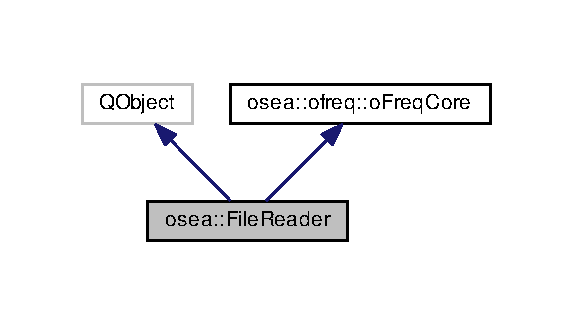
\includegraphics[width=297pt]{classosea_1_1_file_reader__inherit__graph}
\end{center}
\end{figure}
\subsection*{Public Slots}
\begin{DoxyCompactItemize}
\item 
int \hyperlink{classosea_1_1_file_reader_aafe1acb27e25c2774c04c21a808748a4}{read\-Hydro\-File} (std\-::string path)
\begin{DoxyCompactList}\small\item\em Reads hydrodynamic input files. \end{DoxyCompactList}\item 
void \hyperlink{classosea_1_1_file_reader_a54b42892f8c4de66ad1f7bfd1e8e0a27}{set\-System} (\hyperlink{classosea_1_1ofreq_1_1_system}{ofreq\-::\-System} $\ast$pt\-Input)
\begin{DoxyCompactList}\small\item\em Sets the system object for the dictionary to reference. \end{DoxyCompactList}\end{DoxyCompactItemize}
\subsection*{Signals}
\begin{DoxyCompactItemize}
\item 
void \hyperlink{classosea_1_1_file_reader_a705af41cd541f983951b6988082c632c}{output\-Control\-File} (\hyperlink{classosea_1_1_object_group}{Object\-Group} output)
\begin{DoxyCompactList}\small\item\em Sends output of objects discovered when reading the Control file. Top level objects can include\-: \end{DoxyCompactList}\item 
void \hyperlink{classosea_1_1_file_reader_a79f10f1fd00fac75e83152980e34a6ea}{output\-Bodies\-File} (\hyperlink{classosea_1_1_object_group}{Object\-Group} output)
\begin{DoxyCompactList}\small\item\em Sends output of objects discovered when reading the Bodies file. Top level objects can include\-: \end{DoxyCompactList}\item 
void \hyperlink{classosea_1_1_file_reader_a7f061059a96d02e453890e3b6874c17c}{output\-Data\-File} (\hyperlink{classosea_1_1_object_group}{Object\-Group} output)
\begin{DoxyCompactList}\small\item\em Sends output of objects discovered when reading the Data file. Top level objects can include\-: \end{DoxyCompactList}\item 
void \hyperlink{classosea_1_1_file_reader_a02f58d7d0c309a7de4599d5220c3ac65}{output\-Forces\-File} (\hyperlink{classosea_1_1_object_group}{Object\-Group} output)
\begin{DoxyCompactList}\small\item\em Sends output of objects discovered when reading the Forces file. Top level objects can include\-: \end{DoxyCompactList}\item 
void \hyperlink{classosea_1_1_file_reader_a25198e57b3c7f8fbca043ecce848d008}{output\-Sea\-Env\-File} (\hyperlink{classosea_1_1_object_group}{Object\-Group} output)
\begin{DoxyCompactList}\small\item\em Sends output of objects discovered when reading the Sea\-Env file. Top level objects can include\-: \end{DoxyCompactList}\end{DoxyCompactItemize}
\subsection*{Public Member Functions}
\begin{DoxyCompactItemize}
\item 
\hyperlink{classosea_1_1_file_reader_a615dcb2443cad1f2ca123c7c0c334480}{File\-Reader} ()
\begin{DoxyCompactList}\small\item\em Default constructor. \end{DoxyCompactList}\item 
\hyperlink{classosea_1_1_file_reader_a518fc07a4da5ff10374302fd253d3f45}{File\-Reader} (std\-::string Path)
\begin{DoxyCompactList}\small\item\em Constructor with input for file path that holds input files. \end{DoxyCompactList}\item 
\hyperlink{classosea_1_1_file_reader_a1382969e8f1468f3b04ad4b44ab39dee}{$\sim$\-File\-Reader} ()
\item 
void \hyperlink{classosea_1_1_file_reader_a0b12de2af52dc0cdfae5ab337bf494dc}{set\-Path} (std\-::string input)
\begin{DoxyCompactList}\small\item\em Sets the path to the working directory that all control files are located in. \end{DoxyCompactList}\item 
int \hyperlink{classosea_1_1_file_reader_a967cab6ec0822fd8bcf392873a8a82b1}{read\-Control} ()
\begin{DoxyCompactList}\small\item\em Reads in the control file and parses its inputs. \end{DoxyCompactList}\item 
int \hyperlink{classosea_1_1_file_reader_a44770836db4ab430139118727ace6547}{read\-Bodies} ()
\begin{DoxyCompactList}\small\item\em Reads in the Bodies file and parses its inputs. \end{DoxyCompactList}\item 
int \hyperlink{classosea_1_1_file_reader_ab78d2f631eb8e64b0a68d25eeca80be5}{read\-Forces} ()
\begin{DoxyCompactList}\small\item\em Reads in the Forces file and parses its inputs. \end{DoxyCompactList}\item 
int \hyperlink{classosea_1_1_file_reader_a1f8a6bd4b5c53f80cc94d64d6dd1f2da}{read\-Sea\-Env} ()
\begin{DoxyCompactList}\small\item\em Reads in the Sea Environment input file and parses its inputs. \end{DoxyCompactList}\item 
int \hyperlink{classosea_1_1_file_reader_a814f8b06adcc190d4042509797eef6d2}{read\-Data} ()
\begin{DoxyCompactList}\small\item\em Reads in the Data input file and parses its inputs. \end{DoxyCompactList}\item 
void \hyperlink{classosea_1_1_file_reader_a3cbdb7eab632abafcfd055aa92f47b73}{set\-Dictionary} (\hyperlink{classosea_1_1_dictionary}{osea\-::\-Dictionary} \&dict\-In)
\begin{DoxyCompactList}\small\item\em Sets the dictionary object to be used for processing any data read from the input files. \end{DoxyCompactList}\end{DoxyCompactItemize}
\subsection*{Protected Member Functions}
\begin{DoxyCompactItemize}
\item 
void \hyperlink{classosea_1_1_file_reader_aa57b483154b47ad0126d97debb53c638}{send\-Output} (int index)
\begin{DoxyCompactList}\small\item\em Sends the results of parsing the input file onto the dictionary object. Use for processing the input file. \end{DoxyCompactList}\end{DoxyCompactItemize}
\subsection*{Additional Inherited Members}


\subsection{Detailed Description}
\hyperlink{classosea_1_1_file_reader}{File\-Reader} is the next generation of superseded class\-: Read\-Input\-File. \hyperlink{classosea_1_1_file_reader}{File\-Reader} simply reads the text file and parses it into keword value pairs. \hyperlink{classosea_1_1_file_reader}{File\-Reader} reads in the input files. It then passes those input files to the \hyperlink{classosea_1_1_parser}{Parser} object. \hyperlink{classosea_1_1_parser}{Parser} then segments the file in a series of object groupings with a vector list of keyword value pairs. The file reader interprets a limited number of those keywords to recognize new object declarations. It creates the new objects. It then parses the information in that object into a series of keyword-\/value pairs. Each pair is sent to a \hyperlink{classosea_1_1_dictionary}{Dictionary} object that interprets the information. Information is sent using Qt Slots and Signals.

To use this class, the following sequence must be followed. 1.) Create \hyperlink{classosea_1_1_file_reader}{File\-Reader} object. 2.) Create \hyperlink{classosea_1_1_dictionary}{Dictionary} objects for each file type you will read. 3.) Satisfy any follow on dependencies for \hyperlink{classosea_1_1_dictionary}{Dictionary} objects. 4.) Qt Connect \hyperlink{classosea_1_1_file_reader}{File\-Reader} to \hyperlink{classosea_1_1_dictionary}{Dictionary} objects. 5.) Qt Connect \hyperlink{classosea_1_1_file_reader}{File\-Reader} to System object. 6.) Feed in the target path to the \hyperlink{classosea_1_1_file_reader}{File\-Reader} object. 7.) Read each file type in turn. The \hyperlink{classosea_1_1_file_reader}{File\-Reader} object will automatically find the file with the correct filename, read it, parse it, and send the resulting keyword-\/value pairs to the appropriate \hyperlink{classosea_1_1_dictionary}{Dictionary} object. 

Definition at line 105 of file filereader.\-h.



\subsection{Constructor \& Destructor Documentation}
\hypertarget{classosea_1_1_file_reader_a615dcb2443cad1f2ca123c7c0c334480}{\index{osea\-::\-File\-Reader@{osea\-::\-File\-Reader}!File\-Reader@{File\-Reader}}
\index{File\-Reader@{File\-Reader}!osea::FileReader@{osea\-::\-File\-Reader}}
\subsubsection[{File\-Reader}]{\setlength{\rightskip}{0pt plus 5cm}File\-Reader\-::\-File\-Reader (
\begin{DoxyParamCaption}
{}
\end{DoxyParamCaption}
)}}\label{classosea_1_1_file_reader_a615dcb2443cad1f2ca123c7c0c334480}


Default constructor. 



Definition at line 71 of file filereader.\-cpp.

\hypertarget{classosea_1_1_file_reader_a518fc07a4da5ff10374302fd253d3f45}{\index{osea\-::\-File\-Reader@{osea\-::\-File\-Reader}!File\-Reader@{File\-Reader}}
\index{File\-Reader@{File\-Reader}!osea::FileReader@{osea\-::\-File\-Reader}}
\subsubsection[{File\-Reader}]{\setlength{\rightskip}{0pt plus 5cm}osea\-::\-File\-Reader\-::\-File\-Reader (
\begin{DoxyParamCaption}
\item[{std\-::string}]{Path}
\end{DoxyParamCaption}
)}}\label{classosea_1_1_file_reader_a518fc07a4da5ff10374302fd253d3f45}


Constructor with input for file path that holds input files. 


\begin{DoxyParams}{Parameters}
{\em Path} & The full path to the working directory. Variable passed by value. \\
\hline
\end{DoxyParams}
\hypertarget{classosea_1_1_file_reader_a1382969e8f1468f3b04ad4b44ab39dee}{\index{osea\-::\-File\-Reader@{osea\-::\-File\-Reader}!$\sim$\-File\-Reader@{$\sim$\-File\-Reader}}
\index{$\sim$\-File\-Reader@{$\sim$\-File\-Reader}!osea::FileReader@{osea\-::\-File\-Reader}}
\subsubsection[{$\sim$\-File\-Reader}]{\setlength{\rightskip}{0pt plus 5cm}File\-Reader\-::$\sim$\-File\-Reader (
\begin{DoxyParamCaption}
{}
\end{DoxyParamCaption}
)}}\label{classosea_1_1_file_reader_a1382969e8f1468f3b04ad4b44ab39dee}
Default destructor. Nothing happens here. 

Definition at line 84 of file filereader.\-cpp.



\subsection{Member Function Documentation}
\hypertarget{classosea_1_1_file_reader_a79f10f1fd00fac75e83152980e34a6ea}{\index{osea\-::\-File\-Reader@{osea\-::\-File\-Reader}!output\-Bodies\-File@{output\-Bodies\-File}}
\index{output\-Bodies\-File@{output\-Bodies\-File}!osea::FileReader@{osea\-::\-File\-Reader}}
\subsubsection[{output\-Bodies\-File}]{\setlength{\rightskip}{0pt plus 5cm}void osea\-::\-File\-Reader\-::output\-Bodies\-File (
\begin{DoxyParamCaption}
\item[{{\bf Object\-Group}}]{output}
\end{DoxyParamCaption}
)\hspace{0.3cm}{\ttfamily [signal]}}}\label{classosea_1_1_file_reader_a79f10f1fd00fac75e83152980e34a6ea}


Sends output of objects discovered when reading the Bodies file. Top level objects can include\-: 


\begin{DoxyEnumerate}
\item Body object. \begin{DoxySeeAlso}{See Also}
Body 
\end{DoxySeeAlso}

\begin{DoxyParams}{Parameters}
{\em output} & The \hyperlink{classosea_1_1_object_group}{Object\-Group} object parsed out of the file. Variable passed by value. \\
\hline
\end{DoxyParams}

\end{DoxyEnumerate}\hypertarget{classosea_1_1_file_reader_a705af41cd541f983951b6988082c632c}{\index{osea\-::\-File\-Reader@{osea\-::\-File\-Reader}!output\-Control\-File@{output\-Control\-File}}
\index{output\-Control\-File@{output\-Control\-File}!osea::FileReader@{osea\-::\-File\-Reader}}
\subsubsection[{output\-Control\-File}]{\setlength{\rightskip}{0pt plus 5cm}void osea\-::\-File\-Reader\-::output\-Control\-File (
\begin{DoxyParamCaption}
\item[{{\bf Object\-Group}}]{output}
\end{DoxyParamCaption}
)\hspace{0.3cm}{\ttfamily [signal]}}}\label{classosea_1_1_file_reader_a705af41cd541f983951b6988082c632c}


Sends output of objects discovered when reading the Control file. Top level objects can include\-: 


\begin{DoxyEnumerate}
\item System object. \begin{DoxySeeAlso}{See Also}
System 
\end{DoxySeeAlso}

\begin{DoxyParams}{Parameters}
{\em output} & The \hyperlink{classosea_1_1_object_group}{Object\-Group} object parsed out of the file. Variable passed by value. \\
\hline
\end{DoxyParams}

\end{DoxyEnumerate}\hypertarget{classosea_1_1_file_reader_a7f061059a96d02e453890e3b6874c17c}{\index{osea\-::\-File\-Reader@{osea\-::\-File\-Reader}!output\-Data\-File@{output\-Data\-File}}
\index{output\-Data\-File@{output\-Data\-File}!osea::FileReader@{osea\-::\-File\-Reader}}
\subsubsection[{output\-Data\-File}]{\setlength{\rightskip}{0pt plus 5cm}void osea\-::\-File\-Reader\-::output\-Data\-File (
\begin{DoxyParamCaption}
\item[{{\bf Object\-Group}}]{output}
\end{DoxyParamCaption}
)\hspace{0.3cm}{\ttfamily [signal]}}}\label{classosea_1_1_file_reader_a7f061059a96d02e453890e3b6874c17c}


Sends output of objects discovered when reading the Data file. Top level objects can include\-: 


\begin{DoxyEnumerate}
\item hydrofiles 
\begin{DoxyParams}{Parameters}
{\em output} & The \hyperlink{classosea_1_1_object_group}{Object\-Group} object parsed out of the file. Variable passed by value. \\
\hline
\end{DoxyParams}

\end{DoxyEnumerate}\hypertarget{classosea_1_1_file_reader_a02f58d7d0c309a7de4599d5220c3ac65}{\index{osea\-::\-File\-Reader@{osea\-::\-File\-Reader}!output\-Forces\-File@{output\-Forces\-File}}
\index{output\-Forces\-File@{output\-Forces\-File}!osea::FileReader@{osea\-::\-File\-Reader}}
\subsubsection[{output\-Forces\-File}]{\setlength{\rightskip}{0pt plus 5cm}void osea\-::\-File\-Reader\-::output\-Forces\-File (
\begin{DoxyParamCaption}
\item[{{\bf Object\-Group}}]{output}
\end{DoxyParamCaption}
)\hspace{0.3cm}{\ttfamily [signal]}}}\label{classosea_1_1_file_reader_a02f58d7d0c309a7de4599d5220c3ac65}


Sends output of objects discovered when reading the Forces file. Top level objects can include\-: 


\begin{DoxyEnumerate}
\item Force\-Active
\item Force\-Reactive
\item Force\-Cross\-Body \begin{DoxySeeAlso}{See Also}
Force\-Active 

Force\-Cross 

Force\-React 
\end{DoxySeeAlso}

\begin{DoxyParams}{Parameters}
{\em output} & The \hyperlink{classosea_1_1_object_group}{Object\-Group} object parsed out of the file. Variable passed by value. \\
\hline
\end{DoxyParams}

\end{DoxyEnumerate}\hypertarget{classosea_1_1_file_reader_a25198e57b3c7f8fbca043ecce848d008}{\index{osea\-::\-File\-Reader@{osea\-::\-File\-Reader}!output\-Sea\-Env\-File@{output\-Sea\-Env\-File}}
\index{output\-Sea\-Env\-File@{output\-Sea\-Env\-File}!osea::FileReader@{osea\-::\-File\-Reader}}
\subsubsection[{output\-Sea\-Env\-File}]{\setlength{\rightskip}{0pt plus 5cm}void osea\-::\-File\-Reader\-::output\-Sea\-Env\-File (
\begin{DoxyParamCaption}
\item[{{\bf Object\-Group}}]{output}
\end{DoxyParamCaption}
)\hspace{0.3cm}{\ttfamily [signal]}}}\label{classosea_1_1_file_reader_a25198e57b3c7f8fbca043ecce848d008}


Sends output of objects discovered when reading the Sea\-Env file. Top level objects can include\-: 


\begin{DoxyEnumerate}
\item Wave\-\_\-\-Custom
\item Sea\-\_\-\-Custom 
\begin{DoxyParams}{Parameters}
{\em output} & The \hyperlink{classosea_1_1_object_group}{Object\-Group} object parsed out of the file. Variable passed by value. \\
\hline
\end{DoxyParams}

\end{DoxyEnumerate}\hypertarget{classosea_1_1_file_reader_a44770836db4ab430139118727ace6547}{\index{osea\-::\-File\-Reader@{osea\-::\-File\-Reader}!read\-Bodies@{read\-Bodies}}
\index{read\-Bodies@{read\-Bodies}!osea::FileReader@{osea\-::\-File\-Reader}}
\subsubsection[{read\-Bodies}]{\setlength{\rightskip}{0pt plus 5cm}int File\-Reader\-::read\-Bodies (
\begin{DoxyParamCaption}
{}
\end{DoxyParamCaption}
)}}\label{classosea_1_1_file_reader_a44770836db4ab430139118727ace6547}


Reads in the Bodies file and parses its inputs. 

\begin{DoxyReturn}{Returns}
Returns integer to report success or failure of file parsing. Returns 0 for success. Returns 1 for file does not exist. 
\end{DoxyReturn}


Definition at line 124 of file filereader.\-cpp.

\hypertarget{classosea_1_1_file_reader_a967cab6ec0822fd8bcf392873a8a82b1}{\index{osea\-::\-File\-Reader@{osea\-::\-File\-Reader}!read\-Control@{read\-Control}}
\index{read\-Control@{read\-Control}!osea::FileReader@{osea\-::\-File\-Reader}}
\subsubsection[{read\-Control}]{\setlength{\rightskip}{0pt plus 5cm}int File\-Reader\-::read\-Control (
\begin{DoxyParamCaption}
{}
\end{DoxyParamCaption}
)}}\label{classosea_1_1_file_reader_a967cab6ec0822fd8bcf392873a8a82b1}


Reads in the control file and parses its inputs. 

\begin{DoxyReturn}{Returns}
Returns integer to report success or failure of file parsing. Returns 0 for success. Returns 1 for file does not exist. 
\end{DoxyReturn}


Definition at line 104 of file filereader.\-cpp.

\hypertarget{classosea_1_1_file_reader_a814f8b06adcc190d4042509797eef6d2}{\index{osea\-::\-File\-Reader@{osea\-::\-File\-Reader}!read\-Data@{read\-Data}}
\index{read\-Data@{read\-Data}!osea::FileReader@{osea\-::\-File\-Reader}}
\subsubsection[{read\-Data}]{\setlength{\rightskip}{0pt plus 5cm}int File\-Reader\-::read\-Data (
\begin{DoxyParamCaption}
{}
\end{DoxyParamCaption}
)}}\label{classosea_1_1_file_reader_a814f8b06adcc190d4042509797eef6d2}


Reads in the Data input file and parses its inputs. 

\begin{DoxyReturn}{Returns}
Returns integer to report success or failure of file parsing. Returns 0 for success. Returns 1 for file does not exist. 
\end{DoxyReturn}


Definition at line 190 of file filereader.\-cpp.

\hypertarget{classosea_1_1_file_reader_ab78d2f631eb8e64b0a68d25eeca80be5}{\index{osea\-::\-File\-Reader@{osea\-::\-File\-Reader}!read\-Forces@{read\-Forces}}
\index{read\-Forces@{read\-Forces}!osea::FileReader@{osea\-::\-File\-Reader}}
\subsubsection[{read\-Forces}]{\setlength{\rightskip}{0pt plus 5cm}int File\-Reader\-::read\-Forces (
\begin{DoxyParamCaption}
{}
\end{DoxyParamCaption}
)}}\label{classosea_1_1_file_reader_ab78d2f631eb8e64b0a68d25eeca80be5}


Reads in the Forces file and parses its inputs. 

\begin{DoxyReturn}{Returns}
Returns integer to report success or failure of file parsing. Returns 0 for success. Returns 1 for file does not exist. 
\end{DoxyReturn}


Definition at line 150 of file filereader.\-cpp.

\hypertarget{classosea_1_1_file_reader_aafe1acb27e25c2774c04c21a808748a4}{\index{osea\-::\-File\-Reader@{osea\-::\-File\-Reader}!read\-Hydro\-File@{read\-Hydro\-File}}
\index{read\-Hydro\-File@{read\-Hydro\-File}!osea::FileReader@{osea\-::\-File\-Reader}}
\subsubsection[{read\-Hydro\-File}]{\setlength{\rightskip}{0pt plus 5cm}int File\-Reader\-::read\-Hydro\-File (
\begin{DoxyParamCaption}
\item[{std\-::string}]{path}
\end{DoxyParamCaption}
)\hspace{0.3cm}{\ttfamily [slot]}}}\label{classosea_1_1_file_reader_aafe1acb27e25c2774c04c21a808748a4}


Reads hydrodynamic input files. 


\begin{DoxyParams}{Parameters}
{\em path} & The full path to the hydrodynamic input file to read. \\
\hline
\end{DoxyParams}
\begin{DoxyReturn}{Returns}
Returns integer to report success or failure of file parsing. Returns 0 for success. Returns 1 for file does not exist. 
\end{DoxyReturn}


Definition at line 222 of file filereader.\-cpp.

\hypertarget{classosea_1_1_file_reader_a1f8a6bd4b5c53f80cc94d64d6dd1f2da}{\index{osea\-::\-File\-Reader@{osea\-::\-File\-Reader}!read\-Sea\-Env@{read\-Sea\-Env}}
\index{read\-Sea\-Env@{read\-Sea\-Env}!osea::FileReader@{osea\-::\-File\-Reader}}
\subsubsection[{read\-Sea\-Env}]{\setlength{\rightskip}{0pt plus 5cm}int File\-Reader\-::read\-Sea\-Env (
\begin{DoxyParamCaption}
{}
\end{DoxyParamCaption}
)}}\label{classosea_1_1_file_reader_a1f8a6bd4b5c53f80cc94d64d6dd1f2da}


Reads in the Sea Environment input file and parses its inputs. 

\begin{DoxyReturn}{Returns}
Returns integer to report success or failure of file parsing. Returns 0 for success. Returns 1 for file does not exist. 
\end{DoxyReturn}


Definition at line 170 of file filereader.\-cpp.

\hypertarget{classosea_1_1_file_reader_aa57b483154b47ad0126d97debb53c638}{\index{osea\-::\-File\-Reader@{osea\-::\-File\-Reader}!send\-Output@{send\-Output}}
\index{send\-Output@{send\-Output}!osea::FileReader@{osea\-::\-File\-Reader}}
\subsubsection[{send\-Output}]{\setlength{\rightskip}{0pt plus 5cm}void File\-Reader\-::send\-Output (
\begin{DoxyParamCaption}
\item[{int}]{index}
\end{DoxyParamCaption}
)\hspace{0.3cm}{\ttfamily [protected]}}}\label{classosea_1_1_file_reader_aa57b483154b47ad0126d97debb53c638}


Sends the results of parsing the input file onto the dictionary object. Use for processing the input file. 


\begin{DoxyParams}{Parameters}
{\em index} & Integer. The index which specifies which object in the list of recognized objects to use. Variable passed by value. \\
\hline
\end{DoxyParams}


Definition at line 238 of file filereader.\-cpp.

\hypertarget{classosea_1_1_file_reader_a3cbdb7eab632abafcfd055aa92f47b73}{\index{osea\-::\-File\-Reader@{osea\-::\-File\-Reader}!set\-Dictionary@{set\-Dictionary}}
\index{set\-Dictionary@{set\-Dictionary}!osea::FileReader@{osea\-::\-File\-Reader}}
\subsubsection[{set\-Dictionary}]{\setlength{\rightskip}{0pt plus 5cm}void File\-Reader\-::set\-Dictionary (
\begin{DoxyParamCaption}
\item[{{\bf osea\-::\-Dictionary} \&}]{dict\-In}
\end{DoxyParamCaption}
)}}\label{classosea_1_1_file_reader_a3cbdb7eab632abafcfd055aa92f47b73}


Sets the dictionary object to be used for processing any data read from the input files. 


\begin{DoxyParams}{Parameters}
{\em dict\-In} & The dictionary object that you want to use for processing the file. This can change between reading individual files. Variable is passed by reference and stored as a pointer in the object. \\
\hline
\end{DoxyParams}


Definition at line 210 of file filereader.\-cpp.

\hypertarget{classosea_1_1_file_reader_a0b12de2af52dc0cdfae5ab337bf494dc}{\index{osea\-::\-File\-Reader@{osea\-::\-File\-Reader}!set\-Path@{set\-Path}}
\index{set\-Path@{set\-Path}!osea::FileReader@{osea\-::\-File\-Reader}}
\subsubsection[{set\-Path}]{\setlength{\rightskip}{0pt plus 5cm}void File\-Reader\-::set\-Path (
\begin{DoxyParamCaption}
\item[{std\-::string}]{input}
\end{DoxyParamCaption}
)}}\label{classosea_1_1_file_reader_a0b12de2af52dc0cdfae5ab337bf494dc}


Sets the path to the working directory that all control files are located in. 


\begin{DoxyParams}{Parameters}
{\em input} & The full path to the working directory. Do not include directory separator (S\-L\-A\-S\-H, \char`\"{}/\char`\"{}) at end of std\-::string. Variable passed by value. \\
\hline
\end{DoxyParams}


Definition at line 90 of file filereader.\-cpp.

\hypertarget{classosea_1_1_file_reader_a54b42892f8c4de66ad1f7bfd1e8e0a27}{\index{osea\-::\-File\-Reader@{osea\-::\-File\-Reader}!set\-System@{set\-System}}
\index{set\-System@{set\-System}!osea::FileReader@{osea\-::\-File\-Reader}}
\subsubsection[{set\-System}]{\setlength{\rightskip}{0pt plus 5cm}void File\-Reader\-::set\-System (
\begin{DoxyParamCaption}
\item[{{\bf ofreq\-::\-System} $\ast$}]{pt\-Input}
\end{DoxyParamCaption}
)\hspace{0.3cm}{\ttfamily [slot]}}}\label{classosea_1_1_file_reader_a54b42892f8c4de66ad1f7bfd1e8e0a27}


Sets the system object for the dictionary to reference. 


\begin{DoxyParams}{Parameters}
{\em pt\-System} & Pointer to the System object. Variable passed by value. \\
\hline
\end{DoxyParams}


Definition at line 229 of file filereader.\-cpp.



The documentation for this class was generated from the following files\-:\begin{DoxyCompactItemize}
\item 
/home/\-Ship\-\_\-\-Design/\-Projects/\-D\-M\-S1305 Open\-S\-E\-A/master/200\-\_\-src/bin/ofreq/file\-\_\-reader/\hyperlink{filereader_8h}{filereader.\-h}\item 
/home/\-Ship\-\_\-\-Design/\-Projects/\-D\-M\-S1305 Open\-S\-E\-A/master/200\-\_\-src/bin/ofreq/file\-\_\-reader/\hyperlink{filereader_8cpp}{filereader.\-cpp}\end{DoxyCompactItemize}

\hypertarget{classosea_1_1ofreq_1_1_file_writer}{\section{osea\-:\-:ofreq\-:\-:File\-Writer Class Reference}
\label{classosea_1_1ofreq_1_1_file_writer}\index{osea\-::ofreq\-::\-File\-Writer@{osea\-::ofreq\-::\-File\-Writer}}
}


{\ttfamily \#include $<$filewriter.\-h$>$}



Inheritance diagram for osea\-:\-:ofreq\-:\-:File\-Writer\-:
\nopagebreak
\begin{figure}[H]
\begin{center}
\leavevmode
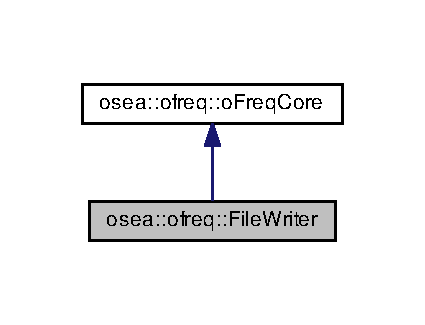
\includegraphics[width=218pt]{classosea_1_1ofreq_1_1_file_writer__inherit__graph}
\end{center}
\end{figure}
\subsection*{Public Member Functions}
\begin{DoxyCompactItemize}
\item 
\hyperlink{classosea_1_1ofreq_1_1_file_writer_aa6b362f5b306dd3409af81a463e97f40}{File\-Writer} ()
\begin{DoxyCompactList}\small\item\em The default constructor. \end{DoxyCompactList}\item 
\hyperlink{classosea_1_1ofreq_1_1_file_writer_aa99ec25b5ed26ad1542eb94104fef1ce}{File\-Writer} (std\-::string root\-Path, \hyperlink{classosea_1_1ofreq_1_1_outputs_body}{Outputs\-Body} \&Body\-In)
\begin{DoxyCompactList}\small\item\em Constructor that includes the two important properties that must be declared for \hyperlink{classosea_1_1ofreq_1_1_file_writer}{File\-Writer} to work correctly. The root path for the project must be declared. And the pointer to the \hyperlink{classosea_1_1ofreq_1_1_outputs_body}{Outputs\-Body} object must be declared. \end{DoxyCompactList}\item 
\hyperlink{classosea_1_1ofreq_1_1_file_writer_ae5490307dcaf9237f4c1b8b8df433e03}{$\sim$\-File\-Writer} ()
\item 
void \hyperlink{classosea_1_1ofreq_1_1_file_writer_aa1dbf0e1a54a78fb62d799187752b002}{set\-Project\-Dir} (std\-::string dir\-In)
\begin{DoxyCompactList}\small\item\em Sets the path to the project directory. Assumes the std\-::string specifying the path does not end with a slash mark. The class will automatically add the slash mark. If a slash mark is present, the function will automatically remove it. \end{DoxyCompactList}\item 
bool \hyperlink{classosea_1_1ofreq_1_1_file_writer_a74a40c3c47b4d12582a2aa44c38d9d07}{clear\-Files} ()
\item 
\hyperlink{classosea_1_1ofreq_1_1_outputs_body}{Outputs\-Body} \& \hyperlink{classosea_1_1ofreq_1_1_file_writer_a77da1b41e1332209f39243fcca4d1287}{ref\-Outputs\-Body} ()
\begin{DoxyCompactList}\small\item\em Provides direct access to the \hyperlink{classosea_1_1ofreq_1_1_outputs_body}{Outputs\-Body} object. The \hyperlink{classosea_1_1ofreq_1_1_outputs_body}{Outputs\-Body} object must be set for the file\-Writer to work. All file data comes from the \hyperlink{classosea_1_1ofreq_1_1_file_writer}{File\-Writer} object. \end{DoxyCompactList}\item 
void \hyperlink{classosea_1_1ofreq_1_1_file_writer_af0234f3573308ca6f5b7178f662b3993}{set\-Outputs\-Body} (\hyperlink{classosea_1_1ofreq_1_1_outputs_body}{Outputs\-Body} $\ast$input)
\begin{DoxyCompactList}\small\item\em Sets the outputs body object, pointer input. \end{DoxyCompactList}\item 
\hyperlink{classosea_1_1ofreq_1_1_outputs_body}{Outputs\-Body} $\ast$ \hyperlink{classosea_1_1ofreq_1_1_file_writer_a2794a9410be184745cd98f26df801ab2}{get\-Outputs\-Body} ()
\begin{DoxyCompactList}\small\item\em Returns a pointer to the Outputs \hyperlink{classosea_1_1ofreq_1_1_body}{Body} object. \end{DoxyCompactList}\item 
bool \hyperlink{classosea_1_1ofreq_1_1_file_writer_afc22f7afcd30f676e5385133247ed84d}{file\-Exists} (std\-::string filename)
\begin{DoxyCompactList}\small\item\em Test is a file exists. Function automatically assumes that the file is located in the directory associated with the \hyperlink{classosea_1_1ofreq_1_1_file_writer_a9748d987475a225b49e14f48b8be0cd6}{get\-Cur\-Wave\-Ind()} function. Returns true if the file exists and is valid. Returns false if the file does not exist or the directory does not exist. \end{DoxyCompactList}\item 
void \hyperlink{classosea_1_1ofreq_1_1_file_writer_a310daaf404e9a0ef1f609eaea85e1bb0}{set\-Header} (std\-::string file\-Path\-In)
\begin{DoxyCompactList}\small\item\em Reads in from input file the header to be used in all files. This is a basic header text that should be at the top of all Open\-S\-E\-A output files. Simple identification of the program. Nothing specific for output. \end{DoxyCompactList}\item 
int \hyperlink{classosea_1_1ofreq_1_1_file_writer_af8b7b6236b90e1734161f6158f64482b}{write\-Wave\-Direction} ()
\begin{DoxyCompactList}\small\item\em Writes the directions list to file. \end{DoxyCompactList}\item 
int \hyperlink{classosea_1_1ofreq_1_1_file_writer_a99e8d1ffb93b50966735bb90d0f4e082}{write\-Frequency} ()
\item 
int \hyperlink{classosea_1_1ofreq_1_1_file_writer_ada34dffe391a0daeac192bd4b7ed0ce5}{write\-Global\-Motion} ()
\begin{DoxyCompactList}\small\item\em Writes the output file of global motions. If file exists, appends to the file, assuming the appended file is a new body object. \end{DoxyCompactList}\item 
int \hyperlink{classosea_1_1ofreq_1_1_file_writer_a9887a28316fca1417da81c95b04c2208}{write\-Global\-Velocity} ()
\begin{DoxyCompactList}\small\item\em Writes the output file of global velocities. If file exists, appends to the file, assuming the appended file is a new body object. \end{DoxyCompactList}\item 
int \hyperlink{classosea_1_1ofreq_1_1_file_writer_a1c49975afb40d028c42027e5239bcdaa}{write\-Global\-Acceleration} ()
\begin{DoxyCompactList}\small\item\em Writes the output file of global accelerations. If file exists, appends to the file, assuming the appended file is a new body object. \end{DoxyCompactList}\item 
int \hyperlink{classosea_1_1ofreq_1_1_file_writer_ae5977c7303f36b1ae0b71bf9251c8a59}{write\-Global\-Solution} ()
\begin{DoxyCompactList}\small\item\em Writes the output file of global solutions. If file exists, appends to the file, assuming the appended file is a new body object. \end{DoxyCompactList}\end{DoxyCompactItemize}
\subsection*{Protected Member Functions}
\begin{DoxyCompactItemize}
\item 
int \hyperlink{classosea_1_1ofreq_1_1_file_writer_a9748d987475a225b49e14f48b8be0cd6}{get\-Cur\-Wave\-Ind} ()
\begin{DoxyCompactList}\small\item\em Gets the index of the current wave direction. The index is used to specify which directory to write the file into. \end{DoxyCompactList}\item 
std\-::string \hyperlink{classosea_1_1ofreq_1_1_file_writer_a82a3acb66bd5c0396836386258608a40}{get\-Cur\-Wave\-Dir} ()
\begin{DoxyCompactList}\small\item\em Returns the std\-::string containing the folder path for the current wave direction. Path name includes the slash mark. For example, if using wave index 0, the std\-::string output would be\-: \char`\"{}d0/\char`\"{}. \end{DoxyCompactList}\item 
bool \hyperlink{classosea_1_1ofreq_1_1_file_writer_ae8deeb9fc4323edf326fb0dadc4f9380}{create\-Dir} (std\-::string path)
\begin{DoxyCompactList}\small\item\em Creates the directory specified by the std\-::string path. Assumes any specified directory is under the root project directory. \end{DoxyCompactList}\item 
std\-::string \hyperlink{classosea_1_1ofreq_1_1_file_writer_a8b2b109105916979fe152960bbadcf7f}{get\-Info\-Block} (std\-::string name\-In)
\end{DoxyCompactItemize}
\subsection*{Additional Inherited Members}


\subsection{Detailed Description}
This class write all outputs to files. All output data is based on the attached \hyperlink{classosea_1_1ofreq_1_1_outputs_body}{Outputs\-Body} object. To use the filewriter object, follow this sequence of steps\-: 1.) Create object. 2.) Set \hyperlink{classosea_1_1ofreq_1_1_outputs_body}{Outputs\-Body} object associated with the file. 3.) Set the filesystem path to the root directory for the current run of ofreq. 4.) Run the \hyperlink{classosea_1_1ofreq_1_1_file_writer_a74a40c3c47b4d12582a2aa44c38d9d07}{clear\-Files()} function, which will clear out any pre-\/existing files. 5.) Run the write\-File function for the specified file that you want to write out.

Note that the \hyperlink{classosea_1_1ofreq_1_1_outputs_body}{Outputs\-Body} object also provides the information on the current wave direction. And the \hyperlink{classosea_1_1ofreq_1_1_file_writer}{File\-Writer} changes its directory to write to depending on the current wave direction. So the \hyperlink{classosea_1_1ofreq_1_1_outputs_body}{Outputs\-Body} object must be updated before writing a new wave direction. 

Definition at line 103 of file filewriter.\-h.



\subsection{Constructor \& Destructor Documentation}
\hypertarget{classosea_1_1ofreq_1_1_file_writer_aa6b362f5b306dd3409af81a463e97f40}{\index{osea\-::ofreq\-::\-File\-Writer@{osea\-::ofreq\-::\-File\-Writer}!File\-Writer@{File\-Writer}}
\index{File\-Writer@{File\-Writer}!osea::ofreq::FileWriter@{osea\-::ofreq\-::\-File\-Writer}}
\subsubsection[{File\-Writer}]{\setlength{\rightskip}{0pt plus 5cm}File\-Writer\-::\-File\-Writer (
\begin{DoxyParamCaption}
{}
\end{DoxyParamCaption}
)}}\label{classosea_1_1ofreq_1_1_file_writer_aa6b362f5b306dd3409af81a463e97f40}


The default constructor. 



Definition at line 89 of file filewriter.\-cpp.

\hypertarget{classosea_1_1ofreq_1_1_file_writer_aa99ec25b5ed26ad1542eb94104fef1ce}{\index{osea\-::ofreq\-::\-File\-Writer@{osea\-::ofreq\-::\-File\-Writer}!File\-Writer@{File\-Writer}}
\index{File\-Writer@{File\-Writer}!osea::ofreq::FileWriter@{osea\-::ofreq\-::\-File\-Writer}}
\subsubsection[{File\-Writer}]{\setlength{\rightskip}{0pt plus 5cm}osea\-::ofreq\-::\-File\-Writer\-::\-File\-Writer (
\begin{DoxyParamCaption}
\item[{std\-::string}]{root\-Path, }
\item[{{\bf Outputs\-Body} \&}]{Body\-In}
\end{DoxyParamCaption}
)}}\label{classosea_1_1ofreq_1_1_file_writer_aa99ec25b5ed26ad1542eb94104fef1ce}


Constructor that includes the two important properties that must be declared for \hyperlink{classosea_1_1ofreq_1_1_file_writer}{File\-Writer} to work correctly. The root path for the project must be declared. And the pointer to the \hyperlink{classosea_1_1ofreq_1_1_outputs_body}{Outputs\-Body} object must be declared. 


\begin{DoxyParams}{Parameters}
{\em root\-Path} & The full fule system path to the root directory of the currently running o\-Freq project. Not the path to the o\-Freq executable files. This is the path to the directory containing input and output files. \\
\hline
{\em Body\-In} & The \hyperlink{classosea_1_1ofreq_1_1_outputs_body}{Outputs\-Body} object that will be used to write out data for the \hyperlink{classosea_1_1ofreq_1_1_file_writer}{File\-Writer}. The \hyperlink{classosea_1_1ofreq_1_1_outputs_body}{Outputs\-Body} object supplies the data, and the \hyperlink{classosea_1_1ofreq_1_1_file_writer}{File\-Writer} writes that data to the A\-S\-C\-I\-I text file. The \hyperlink{classosea_1_1ofreq_1_1_outputs_body}{Outputs\-Body} object also provides the information on the current wave direction. So the \hyperlink{classosea_1_1ofreq_1_1_outputs_body}{Outputs\-Body} object must be updated before writing a new wave direction. \\
\hline
\end{DoxyParams}
\begin{DoxySeeAlso}{See Also}
\hyperlink{classosea_1_1ofreq_1_1_outputs_body}{Outputs\-Body} 
\end{DoxySeeAlso}
\hypertarget{classosea_1_1ofreq_1_1_file_writer_ae5490307dcaf9237f4c1b8b8df433e03}{\index{osea\-::ofreq\-::\-File\-Writer@{osea\-::ofreq\-::\-File\-Writer}!$\sim$\-File\-Writer@{$\sim$\-File\-Writer}}
\index{$\sim$\-File\-Writer@{$\sim$\-File\-Writer}!osea::ofreq::FileWriter@{osea\-::ofreq\-::\-File\-Writer}}
\subsubsection[{$\sim$\-File\-Writer}]{\setlength{\rightskip}{0pt plus 5cm}File\-Writer\-::$\sim$\-File\-Writer (
\begin{DoxyParamCaption}
{}
\end{DoxyParamCaption}
)}}\label{classosea_1_1ofreq_1_1_file_writer_ae5490307dcaf9237f4c1b8b8df433e03}
The default destructor, nothing happens here. 

Definition at line 104 of file filewriter.\-cpp.



\subsection{Member Function Documentation}
\hypertarget{classosea_1_1ofreq_1_1_file_writer_a74a40c3c47b4d12582a2aa44c38d9d07}{\index{osea\-::ofreq\-::\-File\-Writer@{osea\-::ofreq\-::\-File\-Writer}!clear\-Files@{clear\-Files}}
\index{clear\-Files@{clear\-Files}!osea::ofreq::FileWriter@{osea\-::ofreq\-::\-File\-Writer}}
\subsubsection[{clear\-Files}]{\setlength{\rightskip}{0pt plus 5cm}bool File\-Writer\-::clear\-Files (
\begin{DoxyParamCaption}
{}
\end{DoxyParamCaption}
)}}\label{classosea_1_1ofreq_1_1_file_writer_a74a40c3c47b4d12582a2aa44c38d9d07}
Remove all old directiories \& files written by o\-Freq previous run. \begin{DoxyReturn}{Returns}
Return true if all files \& directories were successfully deleted. 
\end{DoxyReturn}


Definition at line 124 of file filewriter.\-cpp.

\hypertarget{classosea_1_1ofreq_1_1_file_writer_ae8deeb9fc4323edf326fb0dadc4f9380}{\index{osea\-::ofreq\-::\-File\-Writer@{osea\-::ofreq\-::\-File\-Writer}!create\-Dir@{create\-Dir}}
\index{create\-Dir@{create\-Dir}!osea::ofreq::FileWriter@{osea\-::ofreq\-::\-File\-Writer}}
\subsubsection[{create\-Dir}]{\setlength{\rightskip}{0pt plus 5cm}bool File\-Writer\-::create\-Dir (
\begin{DoxyParamCaption}
\item[{std\-::string}]{path}
\end{DoxyParamCaption}
)\hspace{0.3cm}{\ttfamily [protected]}}}\label{classosea_1_1ofreq_1_1_file_writer_ae8deeb9fc4323edf326fb0dadc4f9380}


Creates the directory specified by the std\-::string path. Assumes any specified directory is under the root project directory. 


\begin{DoxyParams}{Parameters}
{\em path} & std\-::string. The path of the directory to create. \\
\hline
\end{DoxyParams}
\begin{DoxyReturn}{Returns}
Returns true if creation sucessful. 
\end{DoxyReturn}


Definition at line 858 of file filewriter.\-cpp.

\hypertarget{classosea_1_1ofreq_1_1_file_writer_afc22f7afcd30f676e5385133247ed84d}{\index{osea\-::ofreq\-::\-File\-Writer@{osea\-::ofreq\-::\-File\-Writer}!file\-Exists@{file\-Exists}}
\index{file\-Exists@{file\-Exists}!osea::ofreq::FileWriter@{osea\-::ofreq\-::\-File\-Writer}}
\subsubsection[{file\-Exists}]{\setlength{\rightskip}{0pt plus 5cm}bool File\-Writer\-::file\-Exists (
\begin{DoxyParamCaption}
\item[{std\-::string}]{filename}
\end{DoxyParamCaption}
)}}\label{classosea_1_1ofreq_1_1_file_writer_afc22f7afcd30f676e5385133247ed84d}


Test is a file exists. Function automatically assumes that the file is located in the directory associated with the \hyperlink{classosea_1_1ofreq_1_1_file_writer_a9748d987475a225b49e14f48b8be0cd6}{get\-Cur\-Wave\-Ind()} function. Returns true if the file exists and is valid. Returns false if the file does not exist or the directory does not exist. 


\begin{DoxyParams}{Parameters}
{\em filename} & std\-::string. Specifies the filename to search for. Only needs to specify local filename. Directory information is already inferred from previous settings with the \hyperlink{classosea_1_1ofreq_1_1_outputs_body}{Outputs\-Body} object. \\
\hline
\end{DoxyParams}
\begin{DoxyReturn}{Returns}
Returns boolean variable. True if the file exists. False if the file or any required directories do not exist. 
\end{DoxyReturn}
\begin{DoxySeeAlso}{See Also}
\hyperlink{classosea_1_1ofreq_1_1_file_writer_a9748d987475a225b49e14f48b8be0cd6}{File\-Writer\-::get\-Cur\-Wave\-Ind()} 
\end{DoxySeeAlso}


Definition at line 173 of file filewriter.\-cpp.

\hypertarget{classosea_1_1ofreq_1_1_file_writer_a82a3acb66bd5c0396836386258608a40}{\index{osea\-::ofreq\-::\-File\-Writer@{osea\-::ofreq\-::\-File\-Writer}!get\-Cur\-Wave\-Dir@{get\-Cur\-Wave\-Dir}}
\index{get\-Cur\-Wave\-Dir@{get\-Cur\-Wave\-Dir}!osea::ofreq::FileWriter@{osea\-::ofreq\-::\-File\-Writer}}
\subsubsection[{get\-Cur\-Wave\-Dir}]{\setlength{\rightskip}{0pt plus 5cm}string File\-Writer\-::get\-Cur\-Wave\-Dir (
\begin{DoxyParamCaption}
{}
\end{DoxyParamCaption}
)\hspace{0.3cm}{\ttfamily [protected]}}}\label{classosea_1_1ofreq_1_1_file_writer_a82a3acb66bd5c0396836386258608a40}


Returns the std\-::string containing the folder path for the current wave direction. Path name includes the slash mark. For example, if using wave index 0, the std\-::string output would be\-: \char`\"{}d0/\char`\"{}. 

\begin{DoxyReturn}{Returns}
std\-::string output. Has the path name for the current wave directory. 
\end{DoxyReturn}


Definition at line 848 of file filewriter.\-cpp.

\hypertarget{classosea_1_1ofreq_1_1_file_writer_a9748d987475a225b49e14f48b8be0cd6}{\index{osea\-::ofreq\-::\-File\-Writer@{osea\-::ofreq\-::\-File\-Writer}!get\-Cur\-Wave\-Ind@{get\-Cur\-Wave\-Ind}}
\index{get\-Cur\-Wave\-Ind@{get\-Cur\-Wave\-Ind}!osea::ofreq::FileWriter@{osea\-::ofreq\-::\-File\-Writer}}
\subsubsection[{get\-Cur\-Wave\-Ind}]{\setlength{\rightskip}{0pt plus 5cm}int File\-Writer\-::get\-Cur\-Wave\-Ind (
\begin{DoxyParamCaption}
{}
\end{DoxyParamCaption}
)\hspace{0.3cm}{\ttfamily [protected]}}}\label{classosea_1_1ofreq_1_1_file_writer_a9748d987475a225b49e14f48b8be0cd6}


Gets the index of the current wave direction. The index is used to specify which directory to write the file into. 

\begin{DoxyReturn}{Returns}
Returns integer which specifies the index of the current wave direction. Index specifies the wave direction in the list of wave directions. Valid values are any integer from 0 or greater. 
\end{DoxyReturn}


Definition at line 842 of file filewriter.\-cpp.

\hypertarget{classosea_1_1ofreq_1_1_file_writer_a8b2b109105916979fe152960bbadcf7f}{\index{osea\-::ofreq\-::\-File\-Writer@{osea\-::ofreq\-::\-File\-Writer}!get\-Info\-Block@{get\-Info\-Block}}
\index{get\-Info\-Block@{get\-Info\-Block}!osea::ofreq::FileWriter@{osea\-::ofreq\-::\-File\-Writer}}
\subsubsection[{get\-Info\-Block}]{\setlength{\rightskip}{0pt plus 5cm}string File\-Writer\-::get\-Info\-Block (
\begin{DoxyParamCaption}
\item[{std\-::string}]{name\-In}
\end{DoxyParamCaption}
)\hspace{0.3cm}{\ttfamily [protected]}}}\label{classosea_1_1ofreq_1_1_file_writer_a8b2b109105916979fe152960bbadcf7f}
Set information about the file to be written after header and above data, included in the seafile block. 
\begin{DoxyParams}{Parameters}
{\em name\-In} & The name of the object. \\
\hline
\end{DoxyParams}
\begin{DoxyReturn}{Returns}
Returns std\-::string. std\-::string contains the file info for the output file. Everything written into the seafile block. Variable passed by value. 
\end{DoxyReturn}


Definition at line 873 of file filewriter.\-cpp.

\hypertarget{classosea_1_1ofreq_1_1_file_writer_a2794a9410be184745cd98f26df801ab2}{\index{osea\-::ofreq\-::\-File\-Writer@{osea\-::ofreq\-::\-File\-Writer}!get\-Outputs\-Body@{get\-Outputs\-Body}}
\index{get\-Outputs\-Body@{get\-Outputs\-Body}!osea::ofreq::FileWriter@{osea\-::ofreq\-::\-File\-Writer}}
\subsubsection[{get\-Outputs\-Body}]{\setlength{\rightskip}{0pt plus 5cm}{\bf Outputs\-Body} $\ast$ File\-Writer\-::get\-Outputs\-Body (
\begin{DoxyParamCaption}
{}
\end{DoxyParamCaption}
)}}\label{classosea_1_1ofreq_1_1_file_writer_a2794a9410be184745cd98f26df801ab2}


Returns a pointer to the Outputs \hyperlink{classosea_1_1ofreq_1_1_body}{Body} object. 

\begin{DoxyReturn}{Returns}
Returns a pointer to the Outputs \hyperlink{classosea_1_1ofreq_1_1_body}{Body} object. Returned pointer passed by value. 
\end{DoxyReturn}


Definition at line 167 of file filewriter.\-cpp.

\hypertarget{classosea_1_1ofreq_1_1_file_writer_a77da1b41e1332209f39243fcca4d1287}{\index{osea\-::ofreq\-::\-File\-Writer@{osea\-::ofreq\-::\-File\-Writer}!ref\-Outputs\-Body@{ref\-Outputs\-Body}}
\index{ref\-Outputs\-Body@{ref\-Outputs\-Body}!osea::ofreq::FileWriter@{osea\-::ofreq\-::\-File\-Writer}}
\subsubsection[{ref\-Outputs\-Body}]{\setlength{\rightskip}{0pt plus 5cm}{\bf Outputs\-Body} \& File\-Writer\-::ref\-Outputs\-Body (
\begin{DoxyParamCaption}
{}
\end{DoxyParamCaption}
)}}\label{classosea_1_1ofreq_1_1_file_writer_a77da1b41e1332209f39243fcca4d1287}


Provides direct access to the \hyperlink{classosea_1_1ofreq_1_1_outputs_body}{Outputs\-Body} object. The \hyperlink{classosea_1_1ofreq_1_1_outputs_body}{Outputs\-Body} object must be set for the file\-Writer to work. All file data comes from the \hyperlink{classosea_1_1ofreq_1_1_file_writer}{File\-Writer} object. 

\begin{DoxyReturn}{Returns}
Returns reference to the \hyperlink{classosea_1_1ofreq_1_1_outputs_body}{Outputs\-Body} object. Variable passed by reference. 
\end{DoxyReturn}


Definition at line 155 of file filewriter.\-cpp.

\hypertarget{classosea_1_1ofreq_1_1_file_writer_a310daaf404e9a0ef1f609eaea85e1bb0}{\index{osea\-::ofreq\-::\-File\-Writer@{osea\-::ofreq\-::\-File\-Writer}!set\-Header@{set\-Header}}
\index{set\-Header@{set\-Header}!osea::ofreq::FileWriter@{osea\-::ofreq\-::\-File\-Writer}}
\subsubsection[{set\-Header}]{\setlength{\rightskip}{0pt plus 5cm}void File\-Writer\-::set\-Header (
\begin{DoxyParamCaption}
\item[{std\-::string}]{file\-Path\-In}
\end{DoxyParamCaption}
)}}\label{classosea_1_1ofreq_1_1_file_writer_a310daaf404e9a0ef1f609eaea85e1bb0}


Reads in from input file the header to be used in all files. This is a basic header text that should be at the top of all Open\-S\-E\-A output files. Simple identification of the program. Nothing specific for output. 


\begin{DoxyParams}{Parameters}
{\em file\-Path\-In} & String variable specifying the full location of the folder which has the text for the header file. Header file must be a simple A\-S\-C\-I\-I text file. \\
\hline
\end{DoxyParams}


Definition at line 193 of file filewriter.\-cpp.

\hypertarget{classosea_1_1ofreq_1_1_file_writer_af0234f3573308ca6f5b7178f662b3993}{\index{osea\-::ofreq\-::\-File\-Writer@{osea\-::ofreq\-::\-File\-Writer}!set\-Outputs\-Body@{set\-Outputs\-Body}}
\index{set\-Outputs\-Body@{set\-Outputs\-Body}!osea::ofreq::FileWriter@{osea\-::ofreq\-::\-File\-Writer}}
\subsubsection[{set\-Outputs\-Body}]{\setlength{\rightskip}{0pt plus 5cm}void File\-Writer\-::set\-Outputs\-Body (
\begin{DoxyParamCaption}
\item[{{\bf Outputs\-Body} $\ast$}]{input}
\end{DoxyParamCaption}
)}}\label{classosea_1_1ofreq_1_1_file_writer_af0234f3573308ca6f5b7178f662b3993}


Sets the outputs body object, pointer input. 

Takes a pointer to the Outputs body object as input and stores that pointer for future use. 
\begin{DoxyParams}{Parameters}
{\em input} & Pointer to the Outputs \hyperlink{classosea_1_1ofreq_1_1_body}{Body} object. Pointer variable passed by value. \\
\hline
\end{DoxyParams}


Definition at line 161 of file filewriter.\-cpp.

\hypertarget{classosea_1_1ofreq_1_1_file_writer_aa1dbf0e1a54a78fb62d799187752b002}{\index{osea\-::ofreq\-::\-File\-Writer@{osea\-::ofreq\-::\-File\-Writer}!set\-Project\-Dir@{set\-Project\-Dir}}
\index{set\-Project\-Dir@{set\-Project\-Dir}!osea::ofreq::FileWriter@{osea\-::ofreq\-::\-File\-Writer}}
\subsubsection[{set\-Project\-Dir}]{\setlength{\rightskip}{0pt plus 5cm}void File\-Writer\-::set\-Project\-Dir (
\begin{DoxyParamCaption}
\item[{std\-::string}]{dir\-In}
\end{DoxyParamCaption}
)}}\label{classosea_1_1ofreq_1_1_file_writer_aa1dbf0e1a54a78fb62d799187752b002}


Sets the path to the project directory. Assumes the std\-::string specifying the path does not end with a slash mark. The class will automatically add the slash mark. If a slash mark is present, the function will automatically remove it. 


\begin{DoxyParams}{Parameters}
{\em dir\-In} & std\-::string specifying the path to the project directory. Variable passed by value. \\
\hline
\end{DoxyParams}


Definition at line 110 of file filewriter.\-cpp.

\hypertarget{classosea_1_1ofreq_1_1_file_writer_a99e8d1ffb93b50966735bb90d0f4e082}{\index{osea\-::ofreq\-::\-File\-Writer@{osea\-::ofreq\-::\-File\-Writer}!write\-Frequency@{write\-Frequency}}
\index{write\-Frequency@{write\-Frequency}!osea::ofreq::FileWriter@{osea\-::ofreq\-::\-File\-Writer}}
\subsubsection[{write\-Frequency}]{\setlength{\rightskip}{0pt plus 5cm}int File\-Writer\-::write\-Frequency (
\begin{DoxyParamCaption}
{}
\end{DoxyParamCaption}
)}}\label{classosea_1_1ofreq_1_1_file_writer_a99e8d1ffb93b50966735bb90d0f4e082}
Writes the frequencies list to file. \begin{DoxyReturn}{Returns}
Integer reports status of file writing. Returns of succesful. Otherwise returns a non-\/zero value that is the error code. Returned variable passed by value. 
\end{DoxyReturn}


Definition at line 286 of file filewriter.\-cpp.

\hypertarget{classosea_1_1ofreq_1_1_file_writer_a1c49975afb40d028c42027e5239bcdaa}{\index{osea\-::ofreq\-::\-File\-Writer@{osea\-::ofreq\-::\-File\-Writer}!write\-Global\-Acceleration@{write\-Global\-Acceleration}}
\index{write\-Global\-Acceleration@{write\-Global\-Acceleration}!osea::ofreq::FileWriter@{osea\-::ofreq\-::\-File\-Writer}}
\subsubsection[{write\-Global\-Acceleration}]{\setlength{\rightskip}{0pt plus 5cm}int File\-Writer\-::write\-Global\-Acceleration (
\begin{DoxyParamCaption}
{}
\end{DoxyParamCaption}
)}}\label{classosea_1_1ofreq_1_1_file_writer_a1c49975afb40d028c42027e5239bcdaa}


Writes the output file of global accelerations. If file exists, appends to the file, assuming the appended file is a new body object. 

\begin{DoxyReturn}{Returns}
Integer reports status of file writing. Returns of succesful. Otherwise returns a non-\/zero value that is the error code. Returned variable passed by value. 
\end{DoxyReturn}


Definition at line 589 of file filewriter.\-cpp.

\hypertarget{classosea_1_1ofreq_1_1_file_writer_ada34dffe391a0daeac192bd4b7ed0ce5}{\index{osea\-::ofreq\-::\-File\-Writer@{osea\-::ofreq\-::\-File\-Writer}!write\-Global\-Motion@{write\-Global\-Motion}}
\index{write\-Global\-Motion@{write\-Global\-Motion}!osea::ofreq::FileWriter@{osea\-::ofreq\-::\-File\-Writer}}
\subsubsection[{write\-Global\-Motion}]{\setlength{\rightskip}{0pt plus 5cm}int File\-Writer\-::write\-Global\-Motion (
\begin{DoxyParamCaption}
{}
\end{DoxyParamCaption}
)}}\label{classosea_1_1ofreq_1_1_file_writer_ada34dffe391a0daeac192bd4b7ed0ce5}


Writes the output file of global motions. If file exists, appends to the file, assuming the appended file is a new body object. 

\begin{DoxyReturn}{Returns}
Integer reports status of file writing. Returns of succesful. Otherwise returns a non-\/zero value that is the error code. Returned variable passed by value. 
\end{DoxyReturn}


Definition at line 336 of file filewriter.\-cpp.

\hypertarget{classosea_1_1ofreq_1_1_file_writer_ae5977c7303f36b1ae0b71bf9251c8a59}{\index{osea\-::ofreq\-::\-File\-Writer@{osea\-::ofreq\-::\-File\-Writer}!write\-Global\-Solution@{write\-Global\-Solution}}
\index{write\-Global\-Solution@{write\-Global\-Solution}!osea::ofreq::FileWriter@{osea\-::ofreq\-::\-File\-Writer}}
\subsubsection[{write\-Global\-Solution}]{\setlength{\rightskip}{0pt plus 5cm}int File\-Writer\-::write\-Global\-Solution (
\begin{DoxyParamCaption}
{}
\end{DoxyParamCaption}
)}}\label{classosea_1_1ofreq_1_1_file_writer_ae5977c7303f36b1ae0b71bf9251c8a59}


Writes the output file of global solutions. If file exists, appends to the file, assuming the appended file is a new body object. 

\begin{DoxyReturn}{Returns}
Integer reports status of file writing. Returns of succesful. Otherwise returns a non-\/zero value that is the error code. Returned variable passed by value. 
\end{DoxyReturn}


Definition at line 714 of file filewriter.\-cpp.

\hypertarget{classosea_1_1ofreq_1_1_file_writer_a9887a28316fca1417da81c95b04c2208}{\index{osea\-::ofreq\-::\-File\-Writer@{osea\-::ofreq\-::\-File\-Writer}!write\-Global\-Velocity@{write\-Global\-Velocity}}
\index{write\-Global\-Velocity@{write\-Global\-Velocity}!osea::ofreq::FileWriter@{osea\-::ofreq\-::\-File\-Writer}}
\subsubsection[{write\-Global\-Velocity}]{\setlength{\rightskip}{0pt plus 5cm}int File\-Writer\-::write\-Global\-Velocity (
\begin{DoxyParamCaption}
{}
\end{DoxyParamCaption}
)}}\label{classosea_1_1ofreq_1_1_file_writer_a9887a28316fca1417da81c95b04c2208}


Writes the output file of global velocities. If file exists, appends to the file, assuming the appended file is a new body object. 

\begin{DoxyReturn}{Returns}
Integer reports status of file writing. Returns of succesful. Otherwise returns a non-\/zero value that is the error code. Returned variable passed by value. 
\end{DoxyReturn}


Definition at line 464 of file filewriter.\-cpp.

\hypertarget{classosea_1_1ofreq_1_1_file_writer_af8b7b6236b90e1734161f6158f64482b}{\index{osea\-::ofreq\-::\-File\-Writer@{osea\-::ofreq\-::\-File\-Writer}!write\-Wave\-Direction@{write\-Wave\-Direction}}
\index{write\-Wave\-Direction@{write\-Wave\-Direction}!osea::ofreq::FileWriter@{osea\-::ofreq\-::\-File\-Writer}}
\subsubsection[{write\-Wave\-Direction}]{\setlength{\rightskip}{0pt plus 5cm}int File\-Writer\-::write\-Wave\-Direction (
\begin{DoxyParamCaption}
{}
\end{DoxyParamCaption}
)}}\label{classosea_1_1ofreq_1_1_file_writer_af8b7b6236b90e1734161f6158f64482b}


Writes the directions list to file. 

\begin{DoxyReturn}{Returns}
Integer reports status of file writing. Returns of succesful. Otherwise returns a non-\/zero value that is the error code. Returned variable passed by value. 
\end{DoxyReturn}


Definition at line 236 of file filewriter.\-cpp.



The documentation for this class was generated from the following files\-:\begin{DoxyCompactItemize}
\item 
/home/\-Ship\-\_\-\-Design/\-Projects/\-D\-M\-S1305 Open\-S\-E\-A/master/200\-\_\-src/bin/ofreq/file\-\_\-writer/\hyperlink{filewriter_8h}{filewriter.\-h}\item 
/home/\-Ship\-\_\-\-Design/\-Projects/\-D\-M\-S1305 Open\-S\-E\-A/master/200\-\_\-src/bin/ofreq/file\-\_\-writer/\hyperlink{filewriter_8cpp}{filewriter.\-cpp}\end{DoxyCompactItemize}

\hypertarget{classosea_1_1ofreq_1_1_force}{\section{osea\-:\-:ofreq\-:\-:Force Class Reference}
\label{classosea_1_1ofreq_1_1_force}\index{osea\-::ofreq\-::\-Force@{osea\-::ofreq\-::\-Force}}
}


{\ttfamily \#include $<$force.\-h$>$}



Inheritance diagram for osea\-:\-:ofreq\-:\-:Force\-:
\nopagebreak
\begin{figure}[H]
\begin{center}
\leavevmode
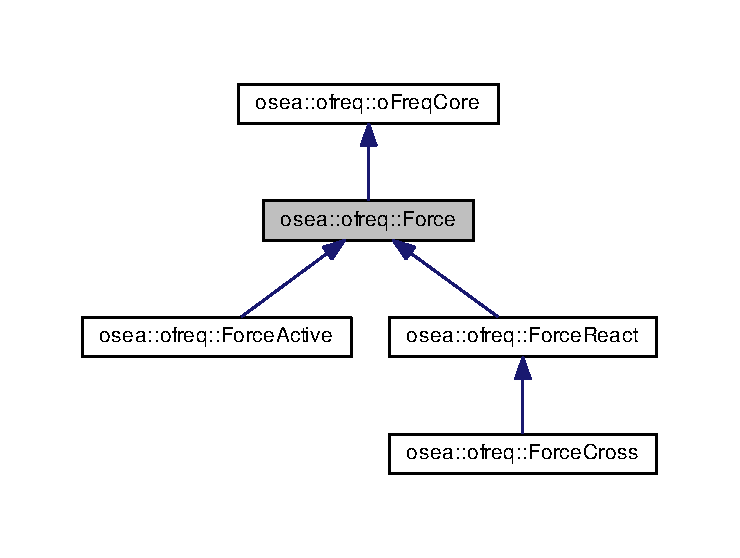
\includegraphics[width=350pt]{classosea_1_1ofreq_1_1_force__inherit__graph}
\end{center}
\end{figure}


Collaboration diagram for osea\-:\-:ofreq\-:\-:Force\-:
\nopagebreak
\begin{figure}[H]
\begin{center}
\leavevmode
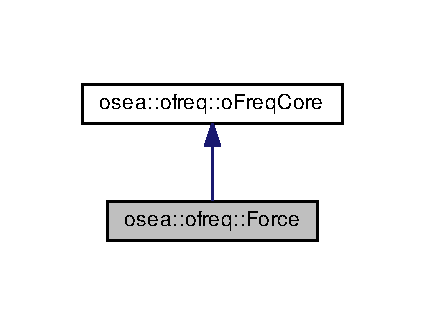
\includegraphics[width=204pt]{classosea_1_1ofreq_1_1_force__coll__graph}
\end{center}
\end{figure}
\subsection*{Public Member Functions}
\begin{DoxyCompactItemize}
\item 
\hyperlink{classosea_1_1ofreq_1_1_force_a00983e3bbc206a00bb9253deafc4e424}{Force} ()
\item 
\hyperlink{classosea_1_1ofreq_1_1_force_a17b130fe437ef6c78162f6d4fb7fc909}{Force} (int index\-In)
\begin{DoxyCompactList}\small\item\em Overloaded constructor for \hyperlink{classosea_1_1ofreq_1_1_force}{Force} object. Allows the \hyperlink{classosea_1_1ofreq_1_1_system}{System} object to pass the index of the newly created \hyperlink{classosea_1_1ofreq_1_1_force}{Force} object in the list of other similar \hyperlink{classosea_1_1ofreq_1_1_force}{Force} objects. Used during object creation for proper association with \hyperlink{classosea_1_1ofreq_1_1_body}{Body} object. \end{DoxyCompactList}\item 
virtual \hyperlink{classosea_1_1ofreq_1_1_force_a8767ca332cee738a462befe1bfbfa454}{$\sim$\-Force} ()
\item 
void \hyperlink{classosea_1_1ofreq_1_1_force_afda991c33f4b65e82b246b24c39f0923}{set\-Force\-Name} (std\-::string)
\item 
std\-::string \hyperlink{classosea_1_1ofreq_1_1_force_a8431fcc0edd27e3edb77f8176bec6908}{get\-Force\-Name} ()
\item 
void \hyperlink{classosea_1_1ofreq_1_1_force_aee052df1c632a6dfb323b5deac443684}{set\-System\-Index} (int index\-In)
\begin{DoxyCompactList}\small\item\em Sets the system index. The index of the \hyperlink{classosea_1_1ofreq_1_1_force}{Force} object as it exists in the list of other similar \hyperlink{classosea_1_1ofreq_1_1_force}{Force} objects contained under the \hyperlink{classosea_1_1ofreq_1_1_system}{System} object. \end{DoxyCompactList}\item 
int \hyperlink{classosea_1_1ofreq_1_1_force_a8cce0e20d734d02c5c52c8ca1f1bde54}{get\-System\-Index} ()
\begin{DoxyCompactList}\small\item\em Gets the system index. The index of the \hyperlink{classosea_1_1ofreq_1_1_force}{Force} object as it exists in the list of other similar \hyperlink{classosea_1_1ofreq_1_1_force}{Force} objects contained under the \hyperlink{classosea_1_1ofreq_1_1_system}{System} object. \end{DoxyCompactList}\end{DoxyCompactItemize}
\subsection*{Protected Attributes}
\begin{DoxyCompactItemize}
\item 
std\-::string \hyperlink{classosea_1_1ofreq_1_1_force_af7cab6c2ebbe013f407570136a5cb8e7}{force\-Name}
\item 
\hypertarget{classosea_1_1ofreq_1_1_force_ae93d98d3c25ed841450d2a839b936aad}{int \hyperlink{classosea_1_1ofreq_1_1_force_ae93d98d3c25ed841450d2a839b936aad}{p\-Sys\-Index}}\label{classosea_1_1ofreq_1_1_force_ae93d98d3c25ed841450d2a839b936aad}

\begin{DoxyCompactList}\small\item\em The index of the \hyperlink{classosea_1_1ofreq_1_1_force}{Force} object as it exists in the list of other similar \hyperlink{classosea_1_1ofreq_1_1_force}{Force} objects contained under the \hyperlink{classosea_1_1ofreq_1_1_system}{System} object. \end{DoxyCompactList}\end{DoxyCompactItemize}
\subsection*{Additional Inherited Members}


\subsection{Detailed Description}
This (base) class holds data for a force object. 

\subsection{Constructor \& Destructor Documentation}
\hypertarget{classosea_1_1ofreq_1_1_force_a00983e3bbc206a00bb9253deafc4e424}{\index{osea\-::ofreq\-::\-Force@{osea\-::ofreq\-::\-Force}!Force@{Force}}
\index{Force@{Force}!osea::ofreq::Force@{osea\-::ofreq\-::\-Force}}
\subsubsection[{Force}]{\setlength{\rightskip}{0pt plus 5cm}Force\-::\-Force (
\begin{DoxyParamCaption}
{}
\end{DoxyParamCaption}
)}}\label{classosea_1_1ofreq_1_1_force_a00983e3bbc206a00bb9253deafc4e424}
The default constructor. \hypertarget{classosea_1_1ofreq_1_1_force_a17b130fe437ef6c78162f6d4fb7fc909}{\index{osea\-::ofreq\-::\-Force@{osea\-::ofreq\-::\-Force}!Force@{Force}}
\index{Force@{Force}!osea::ofreq::Force@{osea\-::ofreq\-::\-Force}}
\subsubsection[{Force}]{\setlength{\rightskip}{0pt plus 5cm}Force\-::\-Force (
\begin{DoxyParamCaption}
\item[{int}]{index\-In}
\end{DoxyParamCaption}
)}}\label{classosea_1_1ofreq_1_1_force_a17b130fe437ef6c78162f6d4fb7fc909}


Overloaded constructor for \hyperlink{classosea_1_1ofreq_1_1_force}{Force} object. Allows the \hyperlink{classosea_1_1ofreq_1_1_system}{System} object to pass the index of the newly created \hyperlink{classosea_1_1ofreq_1_1_force}{Force} object in the list of other similar \hyperlink{classosea_1_1ofreq_1_1_force}{Force} objects. Used during object creation for proper association with \hyperlink{classosea_1_1ofreq_1_1_body}{Body} object. 


\begin{DoxyParams}{Parameters}
{\em index\-In} & Integer. The index of the \hyperlink{classosea_1_1ofreq_1_1_force}{Force} object as it exists in the list of other similar \hyperlink{classosea_1_1ofreq_1_1_force}{Force} objects contained under the \hyperlink{classosea_1_1ofreq_1_1_system}{System} object. Variable passed by value. \\
\hline
\end{DoxyParams}
\begin{DoxySeeAlso}{See Also}
\hyperlink{classosea_1_1ofreq_1_1dict_bodies}{dict\-Bodies} 

\hyperlink{classosea_1_1ofreq_1_1_system}{System} 

\hyperlink{classosea_1_1ofreq_1_1_body}{Body} 
\end{DoxySeeAlso}
\hypertarget{classosea_1_1ofreq_1_1_force_a8767ca332cee738a462befe1bfbfa454}{\index{osea\-::ofreq\-::\-Force@{osea\-::ofreq\-::\-Force}!$\sim$\-Force@{$\sim$\-Force}}
\index{$\sim$\-Force@{$\sim$\-Force}!osea::ofreq::Force@{osea\-::ofreq\-::\-Force}}
\subsubsection[{$\sim$\-Force}]{\setlength{\rightskip}{0pt plus 5cm}Force\-::$\sim$\-Force (
\begin{DoxyParamCaption}
{}
\end{DoxyParamCaption}
)\hspace{0.3cm}{\ttfamily [virtual]}}}\label{classosea_1_1ofreq_1_1_force_a8767ca332cee738a462befe1bfbfa454}
The default destructor, nothing happens here. 

\subsection{Member Function Documentation}
\hypertarget{classosea_1_1ofreq_1_1_force_a8431fcc0edd27e3edb77f8176bec6908}{\index{osea\-::ofreq\-::\-Force@{osea\-::ofreq\-::\-Force}!get\-Force\-Name@{get\-Force\-Name}}
\index{get\-Force\-Name@{get\-Force\-Name}!osea::ofreq::Force@{osea\-::ofreq\-::\-Force}}
\subsubsection[{get\-Force\-Name}]{\setlength{\rightskip}{0pt plus 5cm}string Force\-::get\-Force\-Name (
\begin{DoxyParamCaption}
{}
\end{DoxyParamCaption}
)}}\label{classosea_1_1ofreq_1_1_force_a8431fcc0edd27e3edb77f8176bec6908}
Retrieve the name of the force. \begin{DoxyReturn}{Returns}
new\-Name The name of the force. 
\end{DoxyReturn}
\hypertarget{classosea_1_1ofreq_1_1_force_a8cce0e20d734d02c5c52c8ca1f1bde54}{\index{osea\-::ofreq\-::\-Force@{osea\-::ofreq\-::\-Force}!get\-System\-Index@{get\-System\-Index}}
\index{get\-System\-Index@{get\-System\-Index}!osea::ofreq::Force@{osea\-::ofreq\-::\-Force}}
\subsubsection[{get\-System\-Index}]{\setlength{\rightskip}{0pt plus 5cm}int Force\-::get\-System\-Index (
\begin{DoxyParamCaption}
{}
\end{DoxyParamCaption}
)}}\label{classosea_1_1ofreq_1_1_force_a8cce0e20d734d02c5c52c8ca1f1bde54}


Gets the system index. The index of the \hyperlink{classosea_1_1ofreq_1_1_force}{Force} object as it exists in the list of other similar \hyperlink{classosea_1_1ofreq_1_1_force}{Force} objects contained under the \hyperlink{classosea_1_1ofreq_1_1_system}{System} object. 

\begin{DoxyReturn}{Returns}
Integer. The index of the \hyperlink{classosea_1_1ofreq_1_1_force}{Force} object as it exists in the list of other similar \hyperlink{classosea_1_1ofreq_1_1_force}{Force} objects contained under the \hyperlink{classosea_1_1ofreq_1_1_system}{System} object. Variable passed by value. 
\end{DoxyReturn}
\hypertarget{classosea_1_1ofreq_1_1_force_afda991c33f4b65e82b246b24c39f0923}{\index{osea\-::ofreq\-::\-Force@{osea\-::ofreq\-::\-Force}!set\-Force\-Name@{set\-Force\-Name}}
\index{set\-Force\-Name@{set\-Force\-Name}!osea::ofreq::Force@{osea\-::ofreq\-::\-Force}}
\subsubsection[{set\-Force\-Name}]{\setlength{\rightskip}{0pt plus 5cm}void Force\-::set\-Force\-Name (
\begin{DoxyParamCaption}
\item[{std\-::string}]{}
\end{DoxyParamCaption}
)}}\label{classosea_1_1ofreq_1_1_force_afda991c33f4b65e82b246b24c39f0923}
Sets the name of the force. 
\begin{DoxyParams}{Parameters}
{\em new\-Name} & The name of the force. \\
\hline
\end{DoxyParams}
\hypertarget{classosea_1_1ofreq_1_1_force_aee052df1c632a6dfb323b5deac443684}{\index{osea\-::ofreq\-::\-Force@{osea\-::ofreq\-::\-Force}!set\-System\-Index@{set\-System\-Index}}
\index{set\-System\-Index@{set\-System\-Index}!osea::ofreq::Force@{osea\-::ofreq\-::\-Force}}
\subsubsection[{set\-System\-Index}]{\setlength{\rightskip}{0pt plus 5cm}void Force\-::set\-System\-Index (
\begin{DoxyParamCaption}
\item[{int}]{index\-In}
\end{DoxyParamCaption}
)}}\label{classosea_1_1ofreq_1_1_force_aee052df1c632a6dfb323b5deac443684}


Sets the system index. The index of the \hyperlink{classosea_1_1ofreq_1_1_force}{Force} object as it exists in the list of other similar \hyperlink{classosea_1_1ofreq_1_1_force}{Force} objects contained under the \hyperlink{classosea_1_1ofreq_1_1_system}{System} object. 


\begin{DoxyParams}{Parameters}
{\em index\-In} & Integer. The index of the \hyperlink{classosea_1_1ofreq_1_1_force}{Force} object as it exists in the list of other similar \hyperlink{classosea_1_1ofreq_1_1_force}{Force} objects contained under the \hyperlink{classosea_1_1ofreq_1_1_system}{System} object. Variable passed by value. \\
\hline
\end{DoxyParams}


\subsection{Member Data Documentation}
\hypertarget{classosea_1_1ofreq_1_1_force_af7cab6c2ebbe013f407570136a5cb8e7}{\index{osea\-::ofreq\-::\-Force@{osea\-::ofreq\-::\-Force}!force\-Name@{force\-Name}}
\index{force\-Name@{force\-Name}!osea::ofreq::Force@{osea\-::ofreq\-::\-Force}}
\subsubsection[{force\-Name}]{\setlength{\rightskip}{0pt plus 5cm}std\-::string osea\-::ofreq\-::\-Force\-::force\-Name\hspace{0.3cm}{\ttfamily [protected]}}}\label{classosea_1_1ofreq_1_1_force_af7cab6c2ebbe013f407570136a5cb8e7}
The force name. 

The documentation for this class was generated from the following files\-:\begin{DoxyCompactItemize}
\item 
force.\-h\item 
force.\-cpp\end{DoxyCompactItemize}

\hypertarget{classosea_1_1ofreq_1_1_force_active}{\section{osea\-:\-:ofreq\-:\-:Force\-Active Class Reference}
\label{classosea_1_1ofreq_1_1_force_active}\index{osea\-::ofreq\-::\-Force\-Active@{osea\-::ofreq\-::\-Force\-Active}}
}


{\ttfamily \#include $<$forceactive.\-h$>$}



Inheritance diagram for osea\-:\-:ofreq\-:\-:Force\-Active\-:
\nopagebreak
\begin{figure}[H]
\begin{center}
\leavevmode
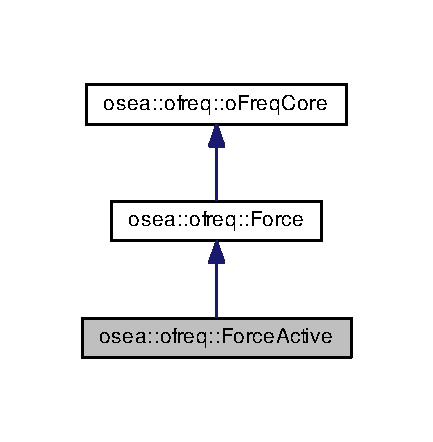
\includegraphics[height=550pt]{classosea_1_1ofreq_1_1_force_active__inherit__graph}
\end{center}
\end{figure}
\subsection*{Public Member Functions}
\begin{DoxyCompactItemize}
\item 
\hyperlink{classosea_1_1ofreq_1_1_force_active_ae006e3394f8c925c6a3218686c5cc8ae}{Force\-Active} ()
\item 
virtual \hyperlink{classosea_1_1ofreq_1_1_force_active_aa2db4bc1fb74ecb6e0ee46c59a40dd2a}{$\sim$\-Force\-Active} ()
\item 
void \hyperlink{classosea_1_1ofreq_1_1_force_active_a488373dc9f5d8f5b07cee3615a2390fe}{set\-Coeff} (std\-::complex$<$ double $>$ coeff\-In, unsigned int index=-\/1)
\begin{DoxyCompactList}\small\item\em Sets the coefficient for the specified index. \end{DoxyCompactList}\item 
void \hyperlink{classosea_1_1ofreq_1_1_force_active_a6c63d2be73033f1c061fd71ce9d58065}{add\-Equation} (std\-::complex$<$ double $>$ eq\-In, int data\-Index=-\/1)
\begin{DoxyCompactList}\small\item\em Adds an equation to the list of equations / coefficients stored in the force\-Active object. \end{DoxyCompactList}\item 
std\-::vector$<$ \hyperlink{namespaceosea_1_1ofreq_a40cad4695a41123a7ae6ab0b6e8b1664}{complex\-Double} $>$ \& \hyperlink{classosea_1_1ofreq_1_1_force_active_a6cc1157859625b457b82ff745f0b5ff4}{list\-Coefficient} ()
\item 
\hyperlink{namespaceosea_1_1ofreq_a40cad4695a41123a7ae6ab0b6e8b1664}{complex\-Double} \& \hyperlink{classosea_1_1ofreq_1_1_force_active_aac0948404f2f21b013b9a02b38087191}{list\-Coefficient} (unsigned int index)
\begin{DoxyCompactList}\small\item\em Provides direct access to a coefficient from the list of coefficients. \end{DoxyCompactList}\item 
std\-::vector$<$ \hyperlink{namespaceosea_1_1ofreq_a40cad4695a41123a7ae6ab0b6e8b1664}{complex\-Double} $>$ \& \hyperlink{classosea_1_1ofreq_1_1_force_active_a6c41c64d60a90442ab2caffcefe703f1}{list\-Data\-Equation} ()
\begin{DoxyCompactList}\small\item\em Another implementation of function list\-Coefficient. But this one uses the Data index. \end{DoxyCompactList}\item 
\hyperlink{namespaceosea_1_1ofreq_a40cad4695a41123a7ae6ab0b6e8b1664}{complex\-Double} \& \hyperlink{classosea_1_1ofreq_1_1_force_active_aa05812dcc8b83df534134888015f75e6}{list\-Data\-Equation} (int index)
\begin{DoxyCompactList}\small\item\em Another implementation of function list\-Coefficient(index). \end{DoxyCompactList}\item 
\hyperlink{namespaceosea_1_1ofreq_a40cad4695a41123a7ae6ab0b6e8b1664}{complex\-Double} \hyperlink{classosea_1_1ofreq_1_1_force_active_a2e01f54c3071d2f8831fb7763cf14500}{get\-Equation} (int number)
\begin{DoxyCompactList}\small\item\em Get a specific number from the list of coefficients. \end{DoxyCompactList}\end{DoxyCompactItemize}
\subsection*{Protected Attributes}
\begin{DoxyCompactItemize}
\item 
std\-::vector$<$ \hyperlink{namespaceosea_1_1ofreq_a40cad4695a41123a7ae6ab0b6e8b1664}{complex\-Double} $>$ \hyperlink{classosea_1_1ofreq_1_1_force_active_af5731f3a699256f0b0b61b77701b236a}{p\-Coefficients}
\item 
std\-::vector$<$ int $>$ \hyperlink{classosea_1_1ofreq_1_1_force_active_a5fe90d49624efff55c2cc641f394f8f4}{p\-Data\-Index}
\begin{DoxyCompactList}\small\item\em The list of data indices for each coefficient. The \hyperlink{classosea_1_1ofreq_1_1_force_active_a6c41c64d60a90442ab2caffcefe703f1}{list\-Data\-Equation()} method will lookup items by their data index, instead of their occurance index in the container vector. This vector contains those data indices used for that search by data\-Index. \end{DoxyCompactList}\end{DoxyCompactItemize}
\subsection*{Additional Inherited Members}


\subsection{Detailed Description}
This class holds data for an active force. 

Definition at line 87 of file forceactive.\-h.



\subsection{Constructor \& Destructor Documentation}
\hypertarget{classosea_1_1ofreq_1_1_force_active_ae006e3394f8c925c6a3218686c5cc8ae}{\index{osea\-::ofreq\-::\-Force\-Active@{osea\-::ofreq\-::\-Force\-Active}!Force\-Active@{Force\-Active}}
\index{Force\-Active@{Force\-Active}!osea::ofreq::ForceActive@{osea\-::ofreq\-::\-Force\-Active}}
\subsubsection[{Force\-Active}]{\setlength{\rightskip}{0pt plus 5cm}Force\-Active\-::\-Force\-Active (
\begin{DoxyParamCaption}
{}
\end{DoxyParamCaption}
)}}\label{classosea_1_1ofreq_1_1_force_active_ae006e3394f8c925c6a3218686c5cc8ae}
The default constructor. 

Definition at line 36 of file forceactive.\-cpp.

\hypertarget{classosea_1_1ofreq_1_1_force_active_aa2db4bc1fb74ecb6e0ee46c59a40dd2a}{\index{osea\-::ofreq\-::\-Force\-Active@{osea\-::ofreq\-::\-Force\-Active}!$\sim$\-Force\-Active@{$\sim$\-Force\-Active}}
\index{$\sim$\-Force\-Active@{$\sim$\-Force\-Active}!osea::ofreq::ForceActive@{osea\-::ofreq\-::\-Force\-Active}}
\subsubsection[{$\sim$\-Force\-Active}]{\setlength{\rightskip}{0pt plus 5cm}Force\-Active\-::$\sim$\-Force\-Active (
\begin{DoxyParamCaption}
{}
\end{DoxyParamCaption}
)\hspace{0.3cm}{\ttfamily [virtual]}}}\label{classosea_1_1ofreq_1_1_force_active_aa2db4bc1fb74ecb6e0ee46c59a40dd2a}
The default destructor, nothing happens here. 

Definition at line 41 of file forceactive.\-cpp.



\subsection{Member Function Documentation}
\hypertarget{classosea_1_1ofreq_1_1_force_active_a6c63d2be73033f1c061fd71ce9d58065}{\index{osea\-::ofreq\-::\-Force\-Active@{osea\-::ofreq\-::\-Force\-Active}!add\-Equation@{add\-Equation}}
\index{add\-Equation@{add\-Equation}!osea::ofreq::ForceActive@{osea\-::ofreq\-::\-Force\-Active}}
\subsubsection[{add\-Equation}]{\setlength{\rightskip}{0pt plus 5cm}void Force\-Active\-::add\-Equation (
\begin{DoxyParamCaption}
\item[{std\-::complex$<$ double $>$}]{eq\-In, }
\item[{int}]{data\-Index = {\ttfamily -\/1}}
\end{DoxyParamCaption}
)}}\label{classosea_1_1ofreq_1_1_force_active_a6c63d2be73033f1c061fd71ce9d58065}


Adds an equation to the list of equations / coefficients stored in the force\-Active object. 

Expands the current list of equations / coefficients by adding the inputs to the end of the list. Adds both the coefficient specified, and the corresponding equation data index. 
\begin{DoxyParams}{Parameters}
{\em eq\-In} & Complex double input. This is the coefficient value stored for the specified equation. Variable passed by value. \\
\hline
{\em data\-Index} & Integer input. This is the data index specified. When objects are retrieved by their data index, they will lookup this value. \\
\hline
\end{DoxyParams}


Definition at line 60 of file forceactive.\-cpp.

\hypertarget{classosea_1_1ofreq_1_1_force_active_a2e01f54c3071d2f8831fb7763cf14500}{\index{osea\-::ofreq\-::\-Force\-Active@{osea\-::ofreq\-::\-Force\-Active}!get\-Equation@{get\-Equation}}
\index{get\-Equation@{get\-Equation}!osea::ofreq::ForceActive@{osea\-::ofreq\-::\-Force\-Active}}
\subsubsection[{get\-Equation}]{\setlength{\rightskip}{0pt plus 5cm}{\bf complex\-Double} Force\-Active\-::get\-Equation (
\begin{DoxyParamCaption}
\item[{int}]{number}
\end{DoxyParamCaption}
)}}\label{classosea_1_1ofreq_1_1_force_active_a2e01f54c3071d2f8831fb7763cf14500}


Get a specific number from the list of coefficients. 

Get a specific number from the list of coefficients. Similar to get\-Coefficients(), only instead of returning the entire vector of coefficients, this only returns a single value in the list. 
\begin{DoxyParams}{Parameters}
{\em number} & Integer specifying which number should be retrieved from the list. \\
\hline
\end{DoxyParams}
\begin{DoxyReturn}{Returns}
Complex Double which is the input coefficient for the active force on the equation specified by number. Returns by value, not by reference. 
\end{DoxyReturn}


Definition at line 123 of file forceactive.\-cpp.

\hypertarget{classosea_1_1ofreq_1_1_force_active_a6cc1157859625b457b82ff745f0b5ff4}{\index{osea\-::ofreq\-::\-Force\-Active@{osea\-::ofreq\-::\-Force\-Active}!list\-Coefficient@{list\-Coefficient}}
\index{list\-Coefficient@{list\-Coefficient}!osea::ofreq::ForceActive@{osea\-::ofreq\-::\-Force\-Active}}
\subsubsection[{list\-Coefficient}]{\setlength{\rightskip}{0pt plus 5cm}vector$<$ {\bf complex\-Double} $>$ \& Force\-Active\-::list\-Coefficient (
\begin{DoxyParamCaption}
{}
\end{DoxyParamCaption}
)}}\label{classosea_1_1ofreq_1_1_force_active_a6cc1157859625b457b82ff745f0b5ff4}
Retrieve the list of coefficients. \begin{DoxyReturn}{Returns}
The list of coefficients. 
\end{DoxyReturn}


Definition at line 77 of file forceactive.\-cpp.

\hypertarget{classosea_1_1ofreq_1_1_force_active_aac0948404f2f21b013b9a02b38087191}{\index{osea\-::ofreq\-::\-Force\-Active@{osea\-::ofreq\-::\-Force\-Active}!list\-Coefficient@{list\-Coefficient}}
\index{list\-Coefficient@{list\-Coefficient}!osea::ofreq::ForceActive@{osea\-::ofreq\-::\-Force\-Active}}
\subsubsection[{list\-Coefficient}]{\setlength{\rightskip}{0pt plus 5cm}{\bf complex\-Double} \& Force\-Active\-::list\-Coefficient (
\begin{DoxyParamCaption}
\item[{unsigned int}]{index}
\end{DoxyParamCaption}
)}}\label{classosea_1_1ofreq_1_1_force_active_aac0948404f2f21b013b9a02b38087191}


Provides direct access to a coefficient from the list of coefficients. 

Returns a value from the list of coefficents. Which value to return is specified by the input index. 
\begin{DoxyParams}{Parameters}
{\em index} & Unsigned integer. Specifies which value to return from the list of coefficients. \\
\hline
\end{DoxyParams}
\begin{DoxyReturn}{Returns}
Returns a complex double. Returned variable is a value from the list of coefficients. Returned variable is passed by reference. 
\end{DoxyReturn}


Definition at line 83 of file forceactive.\-cpp.

\hypertarget{classosea_1_1ofreq_1_1_force_active_a6c41c64d60a90442ab2caffcefe703f1}{\index{osea\-::ofreq\-::\-Force\-Active@{osea\-::ofreq\-::\-Force\-Active}!list\-Data\-Equation@{list\-Data\-Equation}}
\index{list\-Data\-Equation@{list\-Data\-Equation}!osea::ofreq::ForceActive@{osea\-::ofreq\-::\-Force\-Active}}
\subsubsection[{list\-Data\-Equation}]{\setlength{\rightskip}{0pt plus 5cm}vector$<$ {\bf complex\-Double} $>$ \& Force\-Active\-::list\-Data\-Equation (
\begin{DoxyParamCaption}
{}
\end{DoxyParamCaption}
)}}\label{classosea_1_1ofreq_1_1_force_active_a6c41c64d60a90442ab2caffcefe703f1}


Another implementation of function list\-Coefficient. But this one uses the Data index. 

\begin{DoxyReturn}{Returns}
Vector containing the list of coefficients. Argument passed by reference. 
\end{DoxyReturn}


Definition at line 89 of file forceactive.\-cpp.



Here is the call graph for this function\-:\nopagebreak
\begin{figure}[H]
\begin{center}
\leavevmode
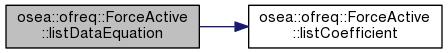
\includegraphics[width=350pt]{classosea_1_1ofreq_1_1_force_active_a6c41c64d60a90442ab2caffcefe703f1_cgraph}
\end{center}
\end{figure}


\hypertarget{classosea_1_1ofreq_1_1_force_active_aa05812dcc8b83df534134888015f75e6}{\index{osea\-::ofreq\-::\-Force\-Active@{osea\-::ofreq\-::\-Force\-Active}!list\-Data\-Equation@{list\-Data\-Equation}}
\index{list\-Data\-Equation@{list\-Data\-Equation}!osea::ofreq::ForceActive@{osea\-::ofreq\-::\-Force\-Active}}
\subsubsection[{list\-Data\-Equation}]{\setlength{\rightskip}{0pt plus 5cm}{\bf complex\-Double} \& Force\-Active\-::list\-Data\-Equation (
\begin{DoxyParamCaption}
\item[{int}]{index}
\end{DoxyParamCaption}
)}}\label{classosea_1_1ofreq_1_1_force_active_aa05812dcc8b83df534134888015f75e6}


Another implementation of function list\-Coefficient(index). 

Provides direct access to items in the list of equations. Returns a single variable from the list of coefficients. Variable is accessed by data index, and not by vector occurrence index. 
\begin{DoxyParams}{Parameters}
{\em index} & Integer. Specifies which value to return from the list of coefficients. \\
\hline
\end{DoxyParams}
\begin{DoxyReturn}{Returns}
Returns a complex double. Returned variable is a value from the list of coefficients. Returned variable is passed by reference. 
\end{DoxyReturn}


Definition at line 95 of file forceactive.\-cpp.

\hypertarget{classosea_1_1ofreq_1_1_force_active_a488373dc9f5d8f5b07cee3615a2390fe}{\index{osea\-::ofreq\-::\-Force\-Active@{osea\-::ofreq\-::\-Force\-Active}!set\-Coeff@{set\-Coeff}}
\index{set\-Coeff@{set\-Coeff}!osea::ofreq::ForceActive@{osea\-::ofreq\-::\-Force\-Active}}
\subsubsection[{set\-Coeff}]{\setlength{\rightskip}{0pt plus 5cm}void Force\-Active\-::set\-Coeff (
\begin{DoxyParamCaption}
\item[{std\-::complex$<$ double $>$}]{coeff\-In, }
\item[{unsigned int}]{index = {\ttfamily -\/1}}
\end{DoxyParamCaption}
)}}\label{classosea_1_1ofreq_1_1_force_active_a488373dc9f5d8f5b07cee3615a2390fe}


Sets the coefficient for the specified index. 


\begin{DoxyParams}{Parameters}
{\em coeff\-In} & The value of the coefficient to specify. Added as a complex number. Variable passed by value. \\
\hline
{\em index} & The equation index of the coefficient to specify. \\
\hline
\end{DoxyParams}


Definition at line 46 of file forceactive.\-cpp.



\subsection{Member Data Documentation}
\hypertarget{classosea_1_1ofreq_1_1_force_active_af5731f3a699256f0b0b61b77701b236a}{\index{osea\-::ofreq\-::\-Force\-Active@{osea\-::ofreq\-::\-Force\-Active}!p\-Coefficients@{p\-Coefficients}}
\index{p\-Coefficients@{p\-Coefficients}!osea::ofreq::ForceActive@{osea\-::ofreq\-::\-Force\-Active}}
\subsubsection[{p\-Coefficients}]{\setlength{\rightskip}{0pt plus 5cm}std\-::vector$<${\bf complex\-Double}$>$ osea\-::ofreq\-::\-Force\-Active\-::p\-Coefficients\hspace{0.3cm}{\ttfamily [protected]}}}\label{classosea_1_1ofreq_1_1_force_active_af5731f3a699256f0b0b61b77701b236a}
The list of force coeffients. 

Definition at line 170 of file forceactive.\-h.

\hypertarget{classosea_1_1ofreq_1_1_force_active_a5fe90d49624efff55c2cc641f394f8f4}{\index{osea\-::ofreq\-::\-Force\-Active@{osea\-::ofreq\-::\-Force\-Active}!p\-Data\-Index@{p\-Data\-Index}}
\index{p\-Data\-Index@{p\-Data\-Index}!osea::ofreq::ForceActive@{osea\-::ofreq\-::\-Force\-Active}}
\subsubsection[{p\-Data\-Index}]{\setlength{\rightskip}{0pt plus 5cm}std\-::vector$<$int$>$ osea\-::ofreq\-::\-Force\-Active\-::p\-Data\-Index\hspace{0.3cm}{\ttfamily [protected]}}}\label{classosea_1_1ofreq_1_1_force_active_a5fe90d49624efff55c2cc641f394f8f4}


The list of data indices for each coefficient. The \hyperlink{classosea_1_1ofreq_1_1_force_active_a6c41c64d60a90442ab2caffcefe703f1}{list\-Data\-Equation()} method will lookup items by their data index, instead of their occurance index in the container vector. This vector contains those data indices used for that search by data\-Index. 



Definition at line 178 of file forceactive.\-h.



The documentation for this class was generated from the following files\-:\begin{DoxyCompactItemize}
\item 
/home/\-Ship\-\_\-\-Design/\-Projects/\-D\-M\-S1305 Open\-S\-E\-A/master/200\-\_\-src/bin/ofreq/global\-\_\-objects/\hyperlink{forceactive_8h}{forceactive.\-h}\item 
/home/\-Ship\-\_\-\-Design/\-Projects/\-D\-M\-S1305 Open\-S\-E\-A/master/200\-\_\-src/bin/ofreq/global\-\_\-objects/\hyperlink{forceactive_8cpp}{forceactive.\-cpp}\end{DoxyCompactItemize}

\hypertarget{classosea_1_1ofreq_1_1_force_cross}{\section{osea\-:\-:ofreq\-:\-:Force\-Cross Class Reference}
\label{classosea_1_1ofreq_1_1_force_cross}\index{osea\-::ofreq\-::\-Force\-Cross@{osea\-::ofreq\-::\-Force\-Cross}}
}


{\ttfamily \#include $<$forcecross.\-h$>$}



Inheritance diagram for osea\-:\-:ofreq\-:\-:Force\-Cross\-:
\nopagebreak
\begin{figure}[H]
\begin{center}
\leavevmode
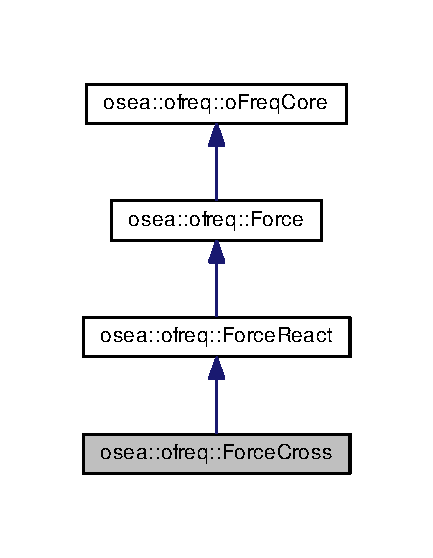
\includegraphics[width=224pt]{classosea_1_1ofreq_1_1_force_cross__inherit__graph}
\end{center}
\end{figure}
\subsection*{Public Member Functions}
\begin{DoxyCompactItemize}
\item 
\hyperlink{classosea_1_1ofreq_1_1_force_cross_a0dd29488051709ddbb950ee75565c53a}{Force\-Cross} ()
\item 
\hyperlink{classosea_1_1ofreq_1_1_force_cross_ad5fc44b9a9d71823f80467f560cfdecc}{$\sim$\-Force\-Cross} ()
\end{DoxyCompactItemize}
\subsection*{Additional Inherited Members}


\subsection{Detailed Description}
This class holds data for a cross body force. A cross body force is very closely related to a reactive force object and they behave almost exactly the same. The only difference is that the force within a reactive force object which is owned by \hyperlink{classosea_1_1ofreq_1_1_body}{Body} A, they are dependant on the motions of that \hyperlink{classosea_1_1ofreq_1_1_body}{Body}. But for a cross-\/body force object\-: The forces from the Cross-\/body force owned by \hyperlink{classosea_1_1ofreq_1_1_body}{Body} A are dependant on the motions of another body. 

Definition at line 85 of file forcecross.\-h.



\subsection{Constructor \& Destructor Documentation}
\hypertarget{classosea_1_1ofreq_1_1_force_cross_a0dd29488051709ddbb950ee75565c53a}{\index{osea\-::ofreq\-::\-Force\-Cross@{osea\-::ofreq\-::\-Force\-Cross}!Force\-Cross@{Force\-Cross}}
\index{Force\-Cross@{Force\-Cross}!osea::ofreq::ForceCross@{osea\-::ofreq\-::\-Force\-Cross}}
\subsubsection[{Force\-Cross}]{\setlength{\rightskip}{0pt plus 5cm}Force\-Cross\-::\-Force\-Cross (
\begin{DoxyParamCaption}
{}
\end{DoxyParamCaption}
)}}\label{classosea_1_1ofreq_1_1_force_cross_a0dd29488051709ddbb950ee75565c53a}
This default constructor creates a \hyperlink{classosea_1_1ofreq_1_1_body}{Body} object. 

Definition at line 32 of file forcecross.\-cpp.

\hypertarget{classosea_1_1ofreq_1_1_force_cross_ad5fc44b9a9d71823f80467f560cfdecc}{\index{osea\-::ofreq\-::\-Force\-Cross@{osea\-::ofreq\-::\-Force\-Cross}!$\sim$\-Force\-Cross@{$\sim$\-Force\-Cross}}
\index{$\sim$\-Force\-Cross@{$\sim$\-Force\-Cross}!osea::ofreq::ForceCross@{osea\-::ofreq\-::\-Force\-Cross}}
\subsubsection[{$\sim$\-Force\-Cross}]{\setlength{\rightskip}{0pt plus 5cm}Force\-Cross\-::$\sim$\-Force\-Cross (
\begin{DoxyParamCaption}
{}
\end{DoxyParamCaption}
)}}\label{classosea_1_1ofreq_1_1_force_cross_ad5fc44b9a9d71823f80467f560cfdecc}
The default destructor, nothing happens here. 

Definition at line 37 of file forcecross.\-cpp.



The documentation for this class was generated from the following files\-:\begin{DoxyCompactItemize}
\item 
/home/\-Ship\-\_\-\-Design/\-Projects/\-D\-M\-S1305 Open\-S\-E\-A/master/200\-\_\-src/bin/ofreq/global\-\_\-objects/\hyperlink{forcecross_8h}{forcecross.\-h}\item 
/home/\-Ship\-\_\-\-Design/\-Projects/\-D\-M\-S1305 Open\-S\-E\-A/master/200\-\_\-src/bin/ofreq/global\-\_\-objects/\hyperlink{forcecross_8cpp}{forcecross.\-cpp}\end{DoxyCompactItemize}

\hypertarget{classosea_1_1ofreq_1_1_force_react}{\section{osea\-:\-:ofreq\-:\-:Force\-React Class Reference}
\label{classosea_1_1ofreq_1_1_force_react}\index{osea\-::ofreq\-::\-Force\-React@{osea\-::ofreq\-::\-Force\-React}}
}


{\ttfamily \#include $<$forcereact.\-h$>$}



Inheritance diagram for osea\-:\-:ofreq\-:\-:Force\-React\-:
\nopagebreak
\begin{figure}[H]
\begin{center}
\leavevmode
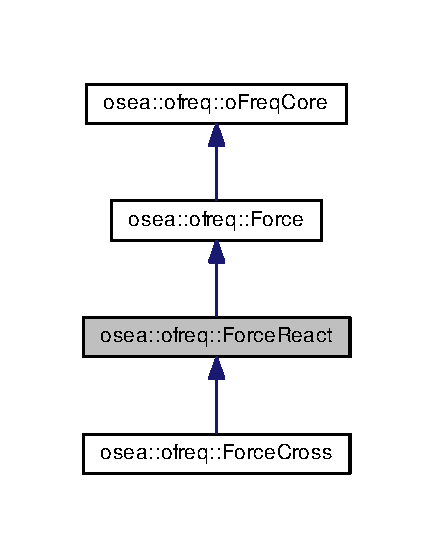
\includegraphics[height=550pt]{classosea_1_1ofreq_1_1_force_react__inherit__graph}
\end{center}
\end{figure}
\subsection*{Public Member Functions}
\begin{DoxyCompactItemize}
\item 
\hyperlink{classosea_1_1ofreq_1_1_force_react_ac8f8b24f67f93f43ae1bb9c464a2d8d4}{Force\-React} ()
\item 
\hyperlink{classosea_1_1ofreq_1_1_force_react_a585f55d5c31c4951824bce98b6582afb}{$\sim$\-Force\-React} ()
\item 
void \hyperlink{classosea_1_1ofreq_1_1_force_react_ac387126f0628a06b24f53012725e384f}{set\-Cur\-Derivative} (int)
\item 
void \hyperlink{classosea_1_1ofreq_1_1_force_react_aca5dc15ce68dd63183aced244c13992c}{set\-Cur\-Equation\-Num} (int)
\item 
std\-::vector$<$ \hyperlink{classosea_1_1ofreq_1_1_derivative}{Derivative} $>$ \& \hyperlink{classosea_1_1ofreq_1_1_force_react_a3c399af8c10b2dbf374c13d85917275e}{list\-Derivative} ()
\begin{DoxyCompactList}\small\item\em Another implementation of get\-Derivatives, under a different name. \end{DoxyCompactList}\item 
\hyperlink{classosea_1_1ofreq_1_1_derivative}{Derivative} \hyperlink{classosea_1_1ofreq_1_1_force_react_aaa5876da8ade31366fc75e3bb5d6ba42}{get\-Derivative} (unsigned int num)
\begin{DoxyCompactList}\small\item\em Retrieve the derivative object specified by the index number. \end{DoxyCompactList}\item 
\hyperlink{classosea_1_1ofreq_1_1_derivative}{Derivative} \& \hyperlink{classosea_1_1ofreq_1_1_force_react_a9966751cff2a417cfe04658a0038aa1b}{list\-Derivative} (unsigned int num)
\begin{DoxyCompactList}\small\item\em Retrieve the derivative object specified by the index number. \end{DoxyCompactList}\item 
void \hyperlink{classosea_1_1ofreq_1_1_force_react_a1aad01d74720d18fd21dd9f70a8b6702}{add\-Derivative} ()
\begin{DoxyCompactList}\small\item\em Adds a \hyperlink{classosea_1_1ofreq_1_1_derivative}{Derivative} object to the list of derivatives. Creates a blank derivative object. Assumed to be the latest order of derivative in the list. \end{DoxyCompactList}\item 
void \hyperlink{classosea_1_1ofreq_1_1_force_react_a7f860f5726f2f9f9baba9775dc72f1ff}{add\-Derivative} (\hyperlink{classosea_1_1ofreq_1_1_derivative}{Derivative} deriv\-In, unsigned int ord\-In)
\begin{DoxyCompactList}\small\item\em Adds a \hyperlink{classosea_1_1ofreq_1_1_derivative}{Derivative} object in the list of derivatives. Sets the new objects as the input for the new derivative object. Uses the properties of the \hyperlink{classosea_1_1ofreq_1_1_derivative}{Derivative} object to set the correct index. \end{DoxyCompactList}\item 
int \hyperlink{classosea_1_1ofreq_1_1_force_react_ae11cdc98d818ca97f710ed13e584c53f}{get\-Max\-Ord} ()
\begin{DoxyCompactList}\small\item\em Returns the maximum order of the derivatives included in the force object. \end{DoxyCompactList}\end{DoxyCompactItemize}
\subsection*{Protected Attributes}
\begin{DoxyCompactItemize}
\item 
std\-::vector$<$ \hyperlink{classosea_1_1ofreq_1_1_derivative}{Derivative} $>$ \hyperlink{classosea_1_1ofreq_1_1_force_react_a28d2bfdc97809181be4d21713cc52181}{p\-Derivative}
\item 
int \hyperlink{classosea_1_1ofreq_1_1_force_react_a56c47ef95ad9ac1876b832dbf75297dd}{current\-Derivative}
\item 
int \hyperlink{classosea_1_1ofreq_1_1_force_react_a35b2a5464dd0135961e04a8389f5967f}{current\-Equation}
\end{DoxyCompactItemize}
\subsection*{Additional Inherited Members}


\subsection{Detailed Description}
This class holds all of the data for a reactive force. 

Definition at line 84 of file forcereact.\-h.



\subsection{Constructor \& Destructor Documentation}
\hypertarget{classosea_1_1ofreq_1_1_force_react_ac8f8b24f67f93f43ae1bb9c464a2d8d4}{\index{osea\-::ofreq\-::\-Force\-React@{osea\-::ofreq\-::\-Force\-React}!Force\-React@{Force\-React}}
\index{Force\-React@{Force\-React}!osea::ofreq::ForceReact@{osea\-::ofreq\-::\-Force\-React}}
\subsubsection[{Force\-React}]{\setlength{\rightskip}{0pt plus 5cm}Force\-React\-::\-Force\-React (
\begin{DoxyParamCaption}
{}
\end{DoxyParamCaption}
)}}\label{classosea_1_1ofreq_1_1_force_react_ac8f8b24f67f93f43ae1bb9c464a2d8d4}
This default constructor. 

Definition at line 33 of file forcereact.\-cpp.

\hypertarget{classosea_1_1ofreq_1_1_force_react_a585f55d5c31c4951824bce98b6582afb}{\index{osea\-::ofreq\-::\-Force\-React@{osea\-::ofreq\-::\-Force\-React}!$\sim$\-Force\-React@{$\sim$\-Force\-React}}
\index{$\sim$\-Force\-React@{$\sim$\-Force\-React}!osea::ofreq::ForceReact@{osea\-::ofreq\-::\-Force\-React}}
\subsubsection[{$\sim$\-Force\-React}]{\setlength{\rightskip}{0pt plus 5cm}Force\-React\-::$\sim$\-Force\-React (
\begin{DoxyParamCaption}
{}
\end{DoxyParamCaption}
)}}\label{classosea_1_1ofreq_1_1_force_react_a585f55d5c31c4951824bce98b6582afb}
The default destructor, nothing happens here. 

Definition at line 37 of file forcereact.\-cpp.



\subsection{Member Function Documentation}
\hypertarget{classosea_1_1ofreq_1_1_force_react_a1aad01d74720d18fd21dd9f70a8b6702}{\index{osea\-::ofreq\-::\-Force\-React@{osea\-::ofreq\-::\-Force\-React}!add\-Derivative@{add\-Derivative}}
\index{add\-Derivative@{add\-Derivative}!osea::ofreq::ForceReact@{osea\-::ofreq\-::\-Force\-React}}
\subsubsection[{add\-Derivative}]{\setlength{\rightskip}{0pt plus 5cm}void Force\-React\-::add\-Derivative (
\begin{DoxyParamCaption}
{}
\end{DoxyParamCaption}
)}}\label{classosea_1_1ofreq_1_1_force_react_a1aad01d74720d18fd21dd9f70a8b6702}


Adds a \hyperlink{classosea_1_1ofreq_1_1_derivative}{Derivative} object to the list of derivatives. Creates a blank derivative object. Assumed to be the latest order of derivative in the list. 



Definition at line 92 of file forcereact.\-cpp.

\hypertarget{classosea_1_1ofreq_1_1_force_react_a7f860f5726f2f9f9baba9775dc72f1ff}{\index{osea\-::ofreq\-::\-Force\-React@{osea\-::ofreq\-::\-Force\-React}!add\-Derivative@{add\-Derivative}}
\index{add\-Derivative@{add\-Derivative}!osea::ofreq::ForceReact@{osea\-::ofreq\-::\-Force\-React}}
\subsubsection[{add\-Derivative}]{\setlength{\rightskip}{0pt plus 5cm}void Force\-React\-::add\-Derivative (
\begin{DoxyParamCaption}
\item[{{\bf Derivative}}]{deriv\-In, }
\item[{unsigned int}]{ord\-In}
\end{DoxyParamCaption}
)}}\label{classosea_1_1ofreq_1_1_force_react_a7f860f5726f2f9f9baba9775dc72f1ff}


Adds a \hyperlink{classosea_1_1ofreq_1_1_derivative}{Derivative} object in the list of derivatives. Sets the new objects as the input for the new derivative object. Uses the properties of the \hyperlink{classosea_1_1ofreq_1_1_derivative}{Derivative} object to set the correct index. 


\begin{DoxyParams}{Parameters}
{\em deriv\-In} & The derivative object to add to the list of derivatives. \\
\hline
{\em ord\-In} & The order of the derivative. \\
\hline
\end{DoxyParams}


Definition at line 99 of file forcereact.\-cpp.

\hypertarget{classosea_1_1ofreq_1_1_force_react_aaa5876da8ade31366fc75e3bb5d6ba42}{\index{osea\-::ofreq\-::\-Force\-React@{osea\-::ofreq\-::\-Force\-React}!get\-Derivative@{get\-Derivative}}
\index{get\-Derivative@{get\-Derivative}!osea::ofreq::ForceReact@{osea\-::ofreq\-::\-Force\-React}}
\subsubsection[{get\-Derivative}]{\setlength{\rightskip}{0pt plus 5cm}{\bf Derivative} Force\-React\-::get\-Derivative (
\begin{DoxyParamCaption}
\item[{unsigned int}]{num}
\end{DoxyParamCaption}
)}}\label{classosea_1_1ofreq_1_1_force_react_aaa5876da8ade31366fc75e3bb5d6ba42}


Retrieve the derivative object specified by the index number. 

Retrieve the derivative object specified by the index number. 
\begin{DoxyParams}{Parameters}
{\em num} & The index number of the derivative object. \\
\hline
\end{DoxyParams}
\begin{DoxyReturn}{Returns}
Returns the derivative object specified by integer num. Returned value is by value. 
\end{DoxyReturn}


Definition at line 59 of file forcereact.\-cpp.

\hypertarget{classosea_1_1ofreq_1_1_force_react_ae11cdc98d818ca97f710ed13e584c53f}{\index{osea\-::ofreq\-::\-Force\-React@{osea\-::ofreq\-::\-Force\-React}!get\-Max\-Ord@{get\-Max\-Ord}}
\index{get\-Max\-Ord@{get\-Max\-Ord}!osea::ofreq::ForceReact@{osea\-::ofreq\-::\-Force\-React}}
\subsubsection[{get\-Max\-Ord}]{\setlength{\rightskip}{0pt plus 5cm}int Force\-React\-::get\-Max\-Ord (
\begin{DoxyParamCaption}
{}
\end{DoxyParamCaption}
)}}\label{classosea_1_1ofreq_1_1_force_react_ae11cdc98d818ca97f710ed13e584c53f}


Returns the maximum order of the derivatives included in the force object. 

Returns the maximum order of the derivatives included in the force object. \begin{DoxyReturn}{Returns}
Returns integer. Returns the maximum order of the derivatives included in the force object. Returned result passed by value. 
\end{DoxyReturn}


Definition at line 115 of file forcereact.\-cpp.

\hypertarget{classosea_1_1ofreq_1_1_force_react_a3c399af8c10b2dbf374c13d85917275e}{\index{osea\-::ofreq\-::\-Force\-React@{osea\-::ofreq\-::\-Force\-React}!list\-Derivative@{list\-Derivative}}
\index{list\-Derivative@{list\-Derivative}!osea::ofreq::ForceReact@{osea\-::ofreq\-::\-Force\-React}}
\subsubsection[{list\-Derivative}]{\setlength{\rightskip}{0pt plus 5cm}vector$<$ {\bf Derivative} $>$ \& Force\-React\-::list\-Derivative (
\begin{DoxyParamCaption}
{}
\end{DoxyParamCaption}
)}}\label{classosea_1_1ofreq_1_1_force_react_a3c399af8c10b2dbf374c13d85917275e}


Another implementation of get\-Derivatives, under a different name. 

\begin{DoxyReturn}{Returns}
Returns the vector of derviative objects. Returned object is by reference. 
\end{DoxyReturn}


Definition at line 53 of file forcereact.\-cpp.

\hypertarget{classosea_1_1ofreq_1_1_force_react_a9966751cff2a417cfe04658a0038aa1b}{\index{osea\-::ofreq\-::\-Force\-React@{osea\-::ofreq\-::\-Force\-React}!list\-Derivative@{list\-Derivative}}
\index{list\-Derivative@{list\-Derivative}!osea::ofreq::ForceReact@{osea\-::ofreq\-::\-Force\-React}}
\subsubsection[{list\-Derivative}]{\setlength{\rightskip}{0pt plus 5cm}{\bf Derivative} \& Force\-React\-::list\-Derivative (
\begin{DoxyParamCaption}
\item[{unsigned int}]{num}
\end{DoxyParamCaption}
)}}\label{classosea_1_1ofreq_1_1_force_react_a9966751cff2a417cfe04658a0038aa1b}


Retrieve the derivative object specified by the index number. 

Retrieve the derivative object specified by the index number. Retrieves a pointer to the derivative object. 
\begin{DoxyParams}{Parameters}
{\em num} & The index number of the derivative object. \\
\hline
\end{DoxyParams}
\begin{DoxyReturn}{Returns}
Returns a pointer to the derivative object specified by integer num. Returned value is by reference. 
\end{DoxyReturn}


Definition at line 75 of file forcereact.\-cpp.

\hypertarget{classosea_1_1ofreq_1_1_force_react_ac387126f0628a06b24f53012725e384f}{\index{osea\-::ofreq\-::\-Force\-React@{osea\-::ofreq\-::\-Force\-React}!set\-Cur\-Derivative@{set\-Cur\-Derivative}}
\index{set\-Cur\-Derivative@{set\-Cur\-Derivative}!osea::ofreq::ForceReact@{osea\-::ofreq\-::\-Force\-React}}
\subsubsection[{set\-Cur\-Derivative}]{\setlength{\rightskip}{0pt plus 5cm}void Force\-React\-::set\-Cur\-Derivative (
\begin{DoxyParamCaption}
\item[{int}]{new\-Order}
\end{DoxyParamCaption}
)}}\label{classosea_1_1ofreq_1_1_force_react_ac387126f0628a06b24f53012725e384f}
Sets the current derivative. 
\begin{DoxyParams}{Parameters}
{\em neworder} & The order of derivative. \\
\hline
\end{DoxyParams}


Definition at line 41 of file forcereact.\-cpp.

\hypertarget{classosea_1_1ofreq_1_1_force_react_aca5dc15ce68dd63183aced244c13992c}{\index{osea\-::ofreq\-::\-Force\-React@{osea\-::ofreq\-::\-Force\-React}!set\-Cur\-Equation\-Num@{set\-Cur\-Equation\-Num}}
\index{set\-Cur\-Equation\-Num@{set\-Cur\-Equation\-Num}!osea::ofreq::ForceReact@{osea\-::ofreq\-::\-Force\-React}}
\subsubsection[{set\-Cur\-Equation\-Num}]{\setlength{\rightskip}{0pt plus 5cm}void Force\-React\-::set\-Cur\-Equation\-Num (
\begin{DoxyParamCaption}
\item[{int}]{new\-Equation\-Num}
\end{DoxyParamCaption}
)}}\label{classosea_1_1ofreq_1_1_force_react_aca5dc15ce68dd63183aced244c13992c}
Sets the current number of the equation. 
\begin{DoxyParams}{Parameters}
{\em new\-Equation\-Num} & The number of the equation. \\
\hline
\end{DoxyParams}


Definition at line 47 of file forcereact.\-cpp.



\subsection{Member Data Documentation}
\hypertarget{classosea_1_1ofreq_1_1_force_react_a56c47ef95ad9ac1876b832dbf75297dd}{\index{osea\-::ofreq\-::\-Force\-React@{osea\-::ofreq\-::\-Force\-React}!current\-Derivative@{current\-Derivative}}
\index{current\-Derivative@{current\-Derivative}!osea::ofreq::ForceReact@{osea\-::ofreq\-::\-Force\-React}}
\subsubsection[{current\-Derivative}]{\setlength{\rightskip}{0pt plus 5cm}int osea\-::ofreq\-::\-Force\-React\-::current\-Derivative\hspace{0.3cm}{\ttfamily [protected]}}}\label{classosea_1_1ofreq_1_1_force_react_a56c47ef95ad9ac1876b832dbf75297dd}
The current order derivative. 

Definition at line 166 of file forcereact.\-h.

\hypertarget{classosea_1_1ofreq_1_1_force_react_a35b2a5464dd0135961e04a8389f5967f}{\index{osea\-::ofreq\-::\-Force\-React@{osea\-::ofreq\-::\-Force\-React}!current\-Equation@{current\-Equation}}
\index{current\-Equation@{current\-Equation}!osea::ofreq::ForceReact@{osea\-::ofreq\-::\-Force\-React}}
\subsubsection[{current\-Equation}]{\setlength{\rightskip}{0pt plus 5cm}int osea\-::ofreq\-::\-Force\-React\-::current\-Equation\hspace{0.3cm}{\ttfamily [protected]}}}\label{classosea_1_1ofreq_1_1_force_react_a35b2a5464dd0135961e04a8389f5967f}
This current equation number. 

Definition at line 167 of file forcereact.\-h.

\hypertarget{classosea_1_1ofreq_1_1_force_react_a28d2bfdc97809181be4d21713cc52181}{\index{osea\-::ofreq\-::\-Force\-React@{osea\-::ofreq\-::\-Force\-React}!p\-Derivative@{p\-Derivative}}
\index{p\-Derivative@{p\-Derivative}!osea::ofreq::ForceReact@{osea\-::ofreq\-::\-Force\-React}}
\subsubsection[{p\-Derivative}]{\setlength{\rightskip}{0pt plus 5cm}std\-::vector$<${\bf Derivative}$>$ osea\-::ofreq\-::\-Force\-React\-::p\-Derivative\hspace{0.3cm}{\ttfamily [protected]}}}\label{classosea_1_1ofreq_1_1_force_react_a28d2bfdc97809181be4d21713cc52181}
This list of derivatives. 

Definition at line 165 of file forcereact.\-h.



The documentation for this class was generated from the following files\-:\begin{DoxyCompactItemize}
\item 
/home/\-Ship\-\_\-\-Design/\-Projects/\-D\-M\-S1305 Open\-S\-E\-A/master/200\-\_\-src/bin/ofreq/global\-\_\-objects/\hyperlink{forcereact_8h}{forcereact.\-h}\item 
/home/\-Ship\-\_\-\-Design/\-Projects/\-D\-M\-S1305 Open\-S\-E\-A/master/200\-\_\-src/bin/ofreq/global\-\_\-objects/\hyperlink{forcereact_8cpp}{forcereact.\-cpp}\end{DoxyCompactItemize}

\hypertarget{classosea_1_1ofreq_1_1_global_acceleration}{\section{osea\-:\-:ofreq\-:\-:Global\-Acceleration Class Reference}
\label{classosea_1_1ofreq_1_1_global_acceleration}\index{osea\-::ofreq\-::\-Global\-Acceleration@{osea\-::ofreq\-::\-Global\-Acceleration}}
}


{\ttfamily \#include $<$globalacceleration.\-h$>$}



Inheritance diagram for osea\-:\-:ofreq\-:\-:Global\-Acceleration\-:
\nopagebreak
\begin{figure}[H]
\begin{center}
\leavevmode
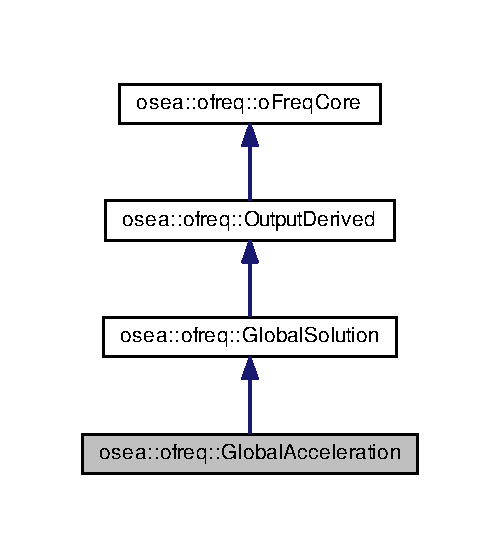
\includegraphics[width=240pt]{classosea_1_1ofreq_1_1_global_acceleration__inherit__graph}
\end{center}
\end{figure}


Collaboration diagram for osea\-:\-:ofreq\-:\-:Global\-Acceleration\-:
\nopagebreak
\begin{figure}[H]
\begin{center}
\leavevmode
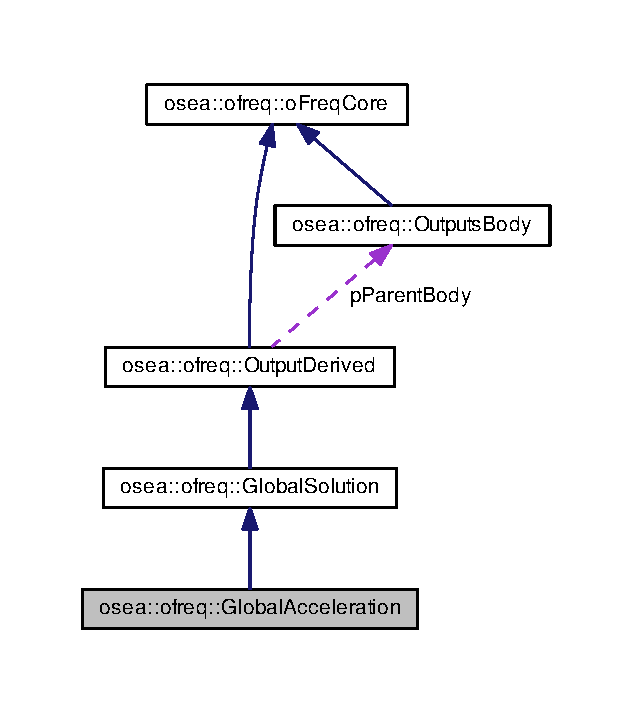
\includegraphics[width=240pt]{classosea_1_1ofreq_1_1_global_acceleration__coll__graph}
\end{center}
\end{figure}
\subsection*{Public Member Functions}
\begin{DoxyCompactItemize}
\item 
\hyperlink{classosea_1_1ofreq_1_1_global_acceleration_a37a05fcecd06641847388428a3f43fb8}{Global\-Acceleration} ()
\item 
\hyperlink{classosea_1_1ofreq_1_1_global_acceleration_aafb7853a1923f0e06b96f2ef4eca03d3}{$\sim$\-Global\-Acceleration} ()
\item 
void \hyperlink{classosea_1_1ofreq_1_1_global_acceleration_a14a041ea42d4c1bc10211c9a44aa3431}{set\-Derivative} (int ord)
\begin{DoxyCompactList}\small\item\em Sets the order of the derivative for the object. \end{DoxyCompactList}\end{DoxyCompactItemize}
\subsection*{Additional Inherited Members}


\subsection{Detailed Description}
This class represents the Global Acceleraion \hyperlink{classosea_1_1ofreq_1_1_solution}{Solution}. 

\subsection{Constructor \& Destructor Documentation}
\hypertarget{classosea_1_1ofreq_1_1_global_acceleration_a37a05fcecd06641847388428a3f43fb8}{\index{osea\-::ofreq\-::\-Global\-Acceleration@{osea\-::ofreq\-::\-Global\-Acceleration}!Global\-Acceleration@{Global\-Acceleration}}
\index{Global\-Acceleration@{Global\-Acceleration}!osea::ofreq::GlobalAcceleration@{osea\-::ofreq\-::\-Global\-Acceleration}}
\subsubsection[{Global\-Acceleration}]{\setlength{\rightskip}{0pt plus 5cm}Global\-Acceleration\-::\-Global\-Acceleration (
\begin{DoxyParamCaption}
{}
\end{DoxyParamCaption}
)}}\label{classosea_1_1ofreq_1_1_global_acceleration_a37a05fcecd06641847388428a3f43fb8}
This default constructor creates a Global Acceleration object. \hypertarget{classosea_1_1ofreq_1_1_global_acceleration_aafb7853a1923f0e06b96f2ef4eca03d3}{\index{osea\-::ofreq\-::\-Global\-Acceleration@{osea\-::ofreq\-::\-Global\-Acceleration}!$\sim$\-Global\-Acceleration@{$\sim$\-Global\-Acceleration}}
\index{$\sim$\-Global\-Acceleration@{$\sim$\-Global\-Acceleration}!osea::ofreq::GlobalAcceleration@{osea\-::ofreq\-::\-Global\-Acceleration}}
\subsubsection[{$\sim$\-Global\-Acceleration}]{\setlength{\rightskip}{0pt plus 5cm}Global\-Acceleration\-::$\sim$\-Global\-Acceleration (
\begin{DoxyParamCaption}
{}
\end{DoxyParamCaption}
)}}\label{classosea_1_1ofreq_1_1_global_acceleration_aafb7853a1923f0e06b96f2ef4eca03d3}
The default destructor, nothing happens here. 

\subsection{Member Function Documentation}
\hypertarget{classosea_1_1ofreq_1_1_global_acceleration_a14a041ea42d4c1bc10211c9a44aa3431}{\index{osea\-::ofreq\-::\-Global\-Acceleration@{osea\-::ofreq\-::\-Global\-Acceleration}!set\-Derivative@{set\-Derivative}}
\index{set\-Derivative@{set\-Derivative}!osea::ofreq::GlobalAcceleration@{osea\-::ofreq\-::\-Global\-Acceleration}}
\subsubsection[{set\-Derivative}]{\setlength{\rightskip}{0pt plus 5cm}void Global\-Acceleration\-::set\-Derivative (
\begin{DoxyParamCaption}
\item[{int}]{ord}
\end{DoxyParamCaption}
)\hspace{0.3cm}{\ttfamily [virtual]}}}\label{classosea_1_1ofreq_1_1_global_acceleration_a14a041ea42d4c1bc10211c9a44aa3431}


Sets the order of the derivative for the object. 


\begin{DoxyParams}{Parameters}
{\em ord} & Integer input that specifies the order of the derivative. Value can be anything from 0 or larger. Variable is passed by value. \\
\hline
\end{DoxyParams}


Reimplemented from \hyperlink{classosea_1_1ofreq_1_1_global_solution_a537163391f1f55d073720b20f69acfa5}{osea\-::ofreq\-::\-Global\-Solution}.



Here is the call graph for this function\-:\nopagebreak
\begin{figure}[H]
\begin{center}
\leavevmode
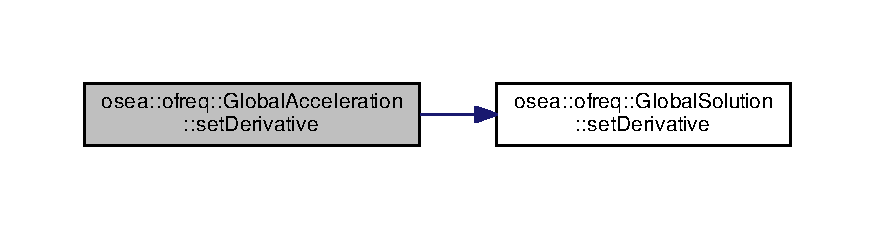
\includegraphics[width=350pt]{classosea_1_1ofreq_1_1_global_acceleration_a14a041ea42d4c1bc10211c9a44aa3431_cgraph}
\end{center}
\end{figure}




The documentation for this class was generated from the following files\-:\begin{DoxyCompactItemize}
\item 
globalacceleration.\-h\item 
globalacceleration.\-cpp\end{DoxyCompactItemize}

\hypertarget{classosea_1_1ofreq_1_1_global_motion}{\section{osea\-:\-:ofreq\-:\-:Global\-Motion Class Reference}
\label{classosea_1_1ofreq_1_1_global_motion}\index{osea\-::ofreq\-::\-Global\-Motion@{osea\-::ofreq\-::\-Global\-Motion}}
}


{\ttfamily \#include $<$globalmotion.\-h$>$}



Inheritance diagram for osea\-:\-:ofreq\-:\-:Global\-Motion\-:\nopagebreak
\begin{figure}[H]
\begin{center}
\leavevmode
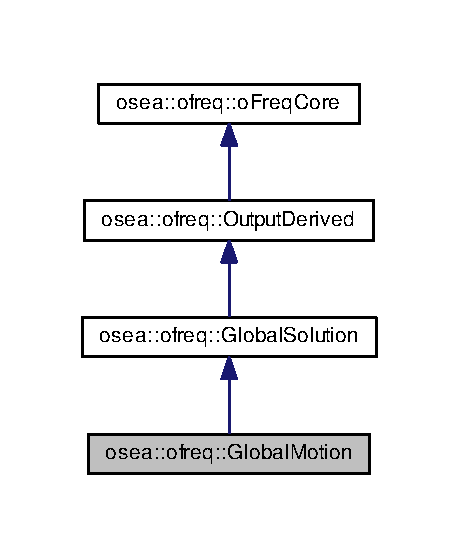
\includegraphics[width=220pt]{classosea_1_1ofreq_1_1_global_motion__inherit__graph}
\end{center}
\end{figure}


Collaboration diagram for osea\-:\-:ofreq\-:\-:Global\-Motion\-:
\nopagebreak
\begin{figure}[H]
\begin{center}
\leavevmode
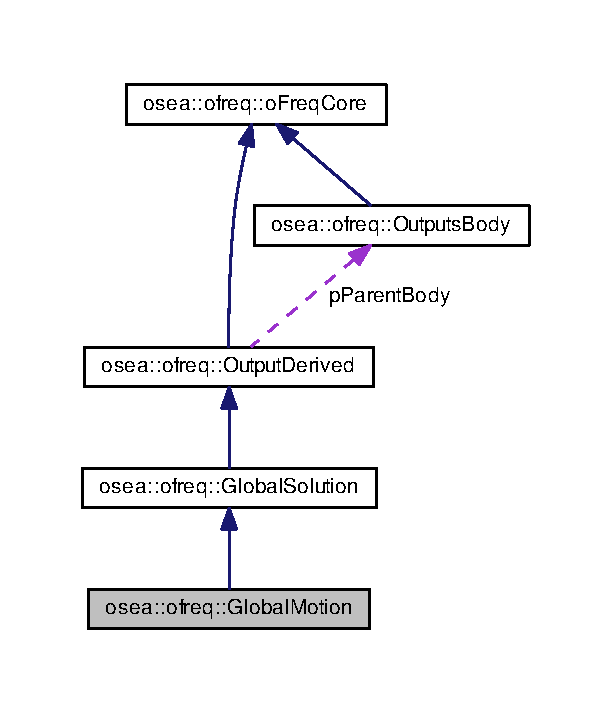
\includegraphics[width=294pt]{classosea_1_1ofreq_1_1_global_motion__coll__graph}
\end{center}
\end{figure}
\subsection*{Public Member Functions}
\begin{DoxyCompactItemize}
\item 
\hyperlink{classosea_1_1ofreq_1_1_global_motion_afe0b801895608782addf27d231bce572}{Global\-Motion} ()
\item 
\hyperlink{classosea_1_1ofreq_1_1_global_motion_ae7155de9b1cb90cbd1d36e7714c1a3ce}{Global\-Motion} (\hyperlink{classosea_1_1ofreq_1_1_outputs_body}{Outputs\-Body} $\ast$input)
\begin{DoxyCompactList}\small\item\em Constructor that also sets the pointer to the \hyperlink{classosea_1_1ofreq_1_1_outputs_body}{Outputs\-Body} object which contains the \hyperlink{classosea_1_1ofreq_1_1_output_derived}{Output\-Derived} object. \end{DoxyCompactList}\item 
\hyperlink{classosea_1_1ofreq_1_1_global_motion_aee21eade3de9cb666a6b8fa42cf1e9e1}{$\sim$\-Global\-Motion} ()
\item 
void \hyperlink{classosea_1_1ofreq_1_1_global_motion_a15a8c0d57ffedf65a1cd84154cdaa6ae}{set\-Derivative} (int ord)
\begin{DoxyCompactList}\small\item\em Sets the order of the derivative for the object. \end{DoxyCompactList}\end{DoxyCompactItemize}
\subsection*{Additional Inherited Members}


\subsection{Detailed Description}
This class represents the Global Motion \hyperlink{classosea_1_1ofreq_1_1_solution}{Solution}. 

\subsection{Constructor \& Destructor Documentation}
\hypertarget{classosea_1_1ofreq_1_1_global_motion_afe0b801895608782addf27d231bce572}{\index{osea\-::ofreq\-::\-Global\-Motion@{osea\-::ofreq\-::\-Global\-Motion}!Global\-Motion@{Global\-Motion}}
\index{Global\-Motion@{Global\-Motion}!osea::ofreq::GlobalMotion@{osea\-::ofreq\-::\-Global\-Motion}}
\subsubsection[{Global\-Motion}]{\setlength{\rightskip}{0pt plus 5cm}Global\-Motion\-::\-Global\-Motion (
\begin{DoxyParamCaption}
{}
\end{DoxyParamCaption}
)}}\label{classosea_1_1ofreq_1_1_global_motion_afe0b801895608782addf27d231bce572}
This default constructor creates a Global Motion object. \hypertarget{classosea_1_1ofreq_1_1_global_motion_ae7155de9b1cb90cbd1d36e7714c1a3ce}{\index{osea\-::ofreq\-::\-Global\-Motion@{osea\-::ofreq\-::\-Global\-Motion}!Global\-Motion@{Global\-Motion}}
\index{Global\-Motion@{Global\-Motion}!osea::ofreq::GlobalMotion@{osea\-::ofreq\-::\-Global\-Motion}}
\subsubsection[{Global\-Motion}]{\setlength{\rightskip}{0pt plus 5cm}Global\-Motion\-::\-Global\-Motion (
\begin{DoxyParamCaption}
\item[{{\bf Outputs\-Body} $\ast$}]{input}
\end{DoxyParamCaption}
)}}\label{classosea_1_1ofreq_1_1_global_motion_ae7155de9b1cb90cbd1d36e7714c1a3ce}


Constructor that also sets the pointer to the \hyperlink{classosea_1_1ofreq_1_1_outputs_body}{Outputs\-Body} object which contains the \hyperlink{classosea_1_1ofreq_1_1_output_derived}{Output\-Derived} object. 


\begin{DoxyParams}{Parameters}
{\em input} & Pointer to the \hyperlink{classosea_1_1ofreq_1_1_outputs_body}{Outputs\-Body} objec that contains this \hyperlink{classosea_1_1ofreq_1_1_output_derived}{Output\-Derived} object. Pointer passed by value.\\
\hline
\end{DoxyParams}
\begin{DoxySeeAlso}{See Also}
set\-Outputs\-Body() 
\end{DoxySeeAlso}
\hypertarget{classosea_1_1ofreq_1_1_global_motion_aee21eade3de9cb666a6b8fa42cf1e9e1}{\index{osea\-::ofreq\-::\-Global\-Motion@{osea\-::ofreq\-::\-Global\-Motion}!$\sim$\-Global\-Motion@{$\sim$\-Global\-Motion}}
\index{$\sim$\-Global\-Motion@{$\sim$\-Global\-Motion}!osea::ofreq::GlobalMotion@{osea\-::ofreq\-::\-Global\-Motion}}
\subsubsection[{$\sim$\-Global\-Motion}]{\setlength{\rightskip}{0pt plus 5cm}Global\-Motion\-::$\sim$\-Global\-Motion (
\begin{DoxyParamCaption}
{}
\end{DoxyParamCaption}
)}}\label{classosea_1_1ofreq_1_1_global_motion_aee21eade3de9cb666a6b8fa42cf1e9e1}
The default destructor, nothing happens here. 

\subsection{Member Function Documentation}
\hypertarget{classosea_1_1ofreq_1_1_global_motion_a15a8c0d57ffedf65a1cd84154cdaa6ae}{\index{osea\-::ofreq\-::\-Global\-Motion@{osea\-::ofreq\-::\-Global\-Motion}!set\-Derivative@{set\-Derivative}}
\index{set\-Derivative@{set\-Derivative}!osea::ofreq::GlobalMotion@{osea\-::ofreq\-::\-Global\-Motion}}
\subsubsection[{set\-Derivative}]{\setlength{\rightskip}{0pt plus 5cm}void Global\-Motion\-::set\-Derivative (
\begin{DoxyParamCaption}
\item[{int}]{ord}
\end{DoxyParamCaption}
)\hspace{0.3cm}{\ttfamily [virtual]}}}\label{classosea_1_1ofreq_1_1_global_motion_a15a8c0d57ffedf65a1cd84154cdaa6ae}


Sets the order of the derivative for the object. 


\begin{DoxyParams}{Parameters}
{\em ord} & Integer input that specifies the order of the derivative. Value can be anything from 0 or larger. Variable is passed by value. \\
\hline
\end{DoxyParams}


Reimplemented from \hyperlink{classosea_1_1ofreq_1_1_global_solution_a537163391f1f55d073720b20f69acfa5}{osea\-::ofreq\-::\-Global\-Solution}.



Here is the call graph for this function\-:\nopagebreak
\begin{figure}[H]
\begin{center}
\leavevmode
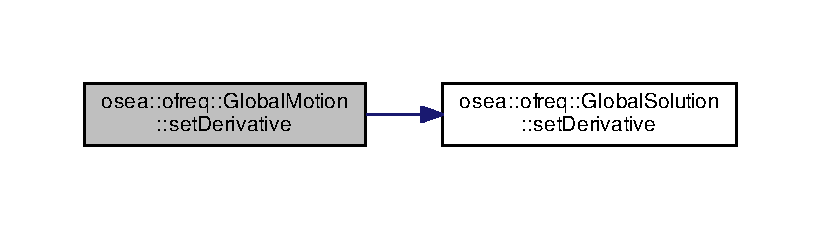
\includegraphics[width=350pt]{classosea_1_1ofreq_1_1_global_motion_a15a8c0d57ffedf65a1cd84154cdaa6ae_cgraph}
\end{center}
\end{figure}




The documentation for this class was generated from the following files\-:\begin{DoxyCompactItemize}
\item 
globalmotion.\-h\item 
globalmotion.\-cpp\end{DoxyCompactItemize}

\hypertarget{classosea_1_1ofreq_1_1_global_solution}{\section{osea\-:\-:ofreq\-:\-:Global\-Solution Class Reference}
\label{classosea_1_1ofreq_1_1_global_solution}\index{osea\-::ofreq\-::\-Global\-Solution@{osea\-::ofreq\-::\-Global\-Solution}}
}


{\ttfamily \#include $<$globalsolution.\-h$>$}



Inheritance diagram for osea\-:\-:ofreq\-:\-:Global\-Solution\-:\nopagebreak
\begin{figure}[H]
\begin{center}
\leavevmode
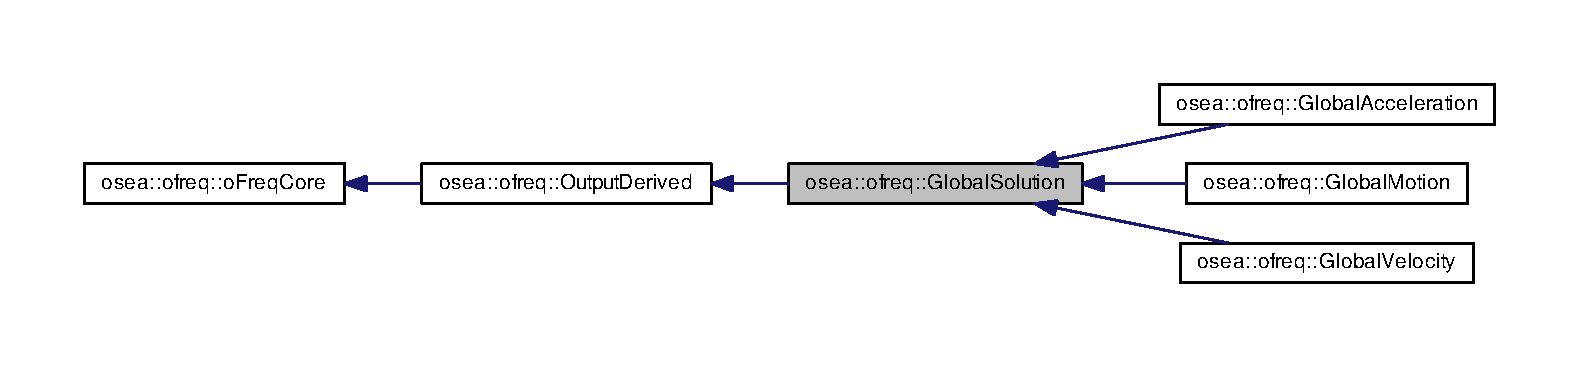
\includegraphics[width=350pt]{classosea_1_1ofreq_1_1_global_solution__inherit__graph}
\end{center}
\end{figure}


Collaboration diagram for osea\-:\-:ofreq\-:\-:Global\-Solution\-:
\nopagebreak
\begin{figure}[H]
\begin{center}
\leavevmode
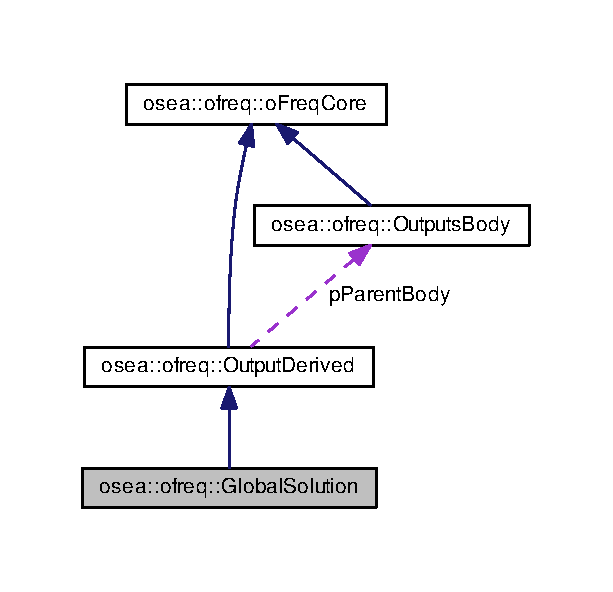
\includegraphics[width=294pt]{classosea_1_1ofreq_1_1_global_solution__coll__graph}
\end{center}
\end{figure}
\subsection*{Public Member Functions}
\begin{DoxyCompactItemize}
\item 
\hyperlink{classosea_1_1ofreq_1_1_global_solution_a27fcfb056c30fc07f8937bc71ec677e6}{Global\-Solution} ()
\item 
\hyperlink{classosea_1_1ofreq_1_1_global_solution_a6ccda8e9eddaddbef8b1fa88f84d42aa}{Global\-Solution} (\hyperlink{classosea_1_1ofreq_1_1_outputs_body}{Outputs\-Body} $\ast$input)
\begin{DoxyCompactList}\small\item\em Constructor that also sets the pointer to the \hyperlink{classosea_1_1ofreq_1_1_outputs_body}{Outputs\-Body} object which contains the \hyperlink{classosea_1_1ofreq_1_1_output_derived}{Output\-Derived} object. \end{DoxyCompactList}\item 
\hyperlink{classosea_1_1ofreq_1_1_global_solution_aea630b237ced06e04c5ea00bf1bb9398}{$\sim$\-Global\-Solution} ()
\item 
virtual void \hyperlink{classosea_1_1ofreq_1_1_global_solution_a537163391f1f55d073720b20f69acfa5}{set\-Derivative} (int ord)
\begin{DoxyCompactList}\small\item\em Sets the order of the derivative for the object. \end{DoxyCompactList}\item 
int \hyperlink{classosea_1_1ofreq_1_1_global_solution_abf8fa956895f2728820d65fda2f5304d}{get\-Derivative} ()
\begin{DoxyCompactList}\small\item\em Gets the order of derivative set for the object. \end{DoxyCompactList}\item 
int \hyperlink{classosea_1_1ofreq_1_1_global_solution_ac9e36cb3ec2beb4a308466fab0263714}{calc\-Output} (int freq\-In)
\begin{DoxyCompactList}\small\item\em Calculates the \hyperlink{classosea_1_1ofreq_1_1_global_solution}{Global\-Solution} output. \hyperlink{classosea_1_1ofreq_1_1_global_solution}{Global\-Solution} is the direct output of the solution for each body, translated into body coordinates. The output is modified to provide the specified order of derivative for the solution. \end{DoxyCompactList}\end{DoxyCompactItemize}
\subsection*{Protected Member Functions}
\begin{DoxyCompactItemize}
\item 
\hyperlink{classosea_1_1ofreq_1_1_solution}{Solution} \& \hyperlink{classosea_1_1ofreq_1_1_global_solution_a43a8caad9f88e3b468c3e9a364b45500}{get\-Solution} (double freq\-In)
\begin{DoxyCompactList}\small\item\em Gets the solution matrix to perform operations on. Accesses the solution matrix from the parent body. \end{DoxyCompactList}\end{DoxyCompactItemize}
\subsection*{Protected Attributes}
\begin{DoxyCompactItemize}
\item 
\hypertarget{classosea_1_1ofreq_1_1_global_solution_a935843ad9f4fd2de2a2ec407de45a20d}{int \hyperlink{classosea_1_1ofreq_1_1_global_solution_a935843ad9f4fd2de2a2ec407de45a20d}{order\-Derivative}}\label{classosea_1_1ofreq_1_1_global_solution_a935843ad9f4fd2de2a2ec407de45a20d}

\begin{DoxyCompactList}\small\item\em The order of derivative to use for calculating output. Set by child classes for specifying specific outputs. \end{DoxyCompactList}\end{DoxyCompactItemize}
\subsection*{Additional Inherited Members}


\subsection{Detailed Description}
This class represents the Global \hyperlink{classosea_1_1ofreq_1_1_solution}{Solution}. The Global \hyperlink{classosea_1_1ofreq_1_1_solution}{Solution} is the direct output of the solved values for each body. It provides the motions calculated for each body, translated back to body coordinate system. The \hyperlink{classosea_1_1ofreq_1_1_global_solution}{Global\-Solution} can output any desired derivative of the solved motions. Several other child classes are derived from this class. The only difference is that for those other classes, the order of derivative is predefined. \begin{DoxySeeAlso}{See Also}
\hyperlink{classosea_1_1ofreq_1_1_global_motion}{Global\-Motion} 

\hyperlink{classosea_1_1ofreq_1_1_global_velocity}{Global\-Velocity} 

\hyperlink{classosea_1_1ofreq_1_1_global_acceleration}{Global\-Acceleration} 
\end{DoxySeeAlso}


\subsection{Constructor \& Destructor Documentation}
\hypertarget{classosea_1_1ofreq_1_1_global_solution_a27fcfb056c30fc07f8937bc71ec677e6}{\index{osea\-::ofreq\-::\-Global\-Solution@{osea\-::ofreq\-::\-Global\-Solution}!Global\-Solution@{Global\-Solution}}
\index{Global\-Solution@{Global\-Solution}!osea::ofreq::GlobalSolution@{osea\-::ofreq\-::\-Global\-Solution}}
\subsubsection[{Global\-Solution}]{\setlength{\rightskip}{0pt plus 5cm}Global\-Solution\-::\-Global\-Solution (
\begin{DoxyParamCaption}
{}
\end{DoxyParamCaption}
)}}\label{classosea_1_1ofreq_1_1_global_solution_a27fcfb056c30fc07f8937bc71ec677e6}
This default constructor creates a Global \hyperlink{classosea_1_1ofreq_1_1_solution}{Solution} object. \hypertarget{classosea_1_1ofreq_1_1_global_solution_a6ccda8e9eddaddbef8b1fa88f84d42aa}{\index{osea\-::ofreq\-::\-Global\-Solution@{osea\-::ofreq\-::\-Global\-Solution}!Global\-Solution@{Global\-Solution}}
\index{Global\-Solution@{Global\-Solution}!osea::ofreq::GlobalSolution@{osea\-::ofreq\-::\-Global\-Solution}}
\subsubsection[{Global\-Solution}]{\setlength{\rightskip}{0pt plus 5cm}Global\-Solution\-::\-Global\-Solution (
\begin{DoxyParamCaption}
\item[{{\bf Outputs\-Body} $\ast$}]{input}
\end{DoxyParamCaption}
)}}\label{classosea_1_1ofreq_1_1_global_solution_a6ccda8e9eddaddbef8b1fa88f84d42aa}


Constructor that also sets the pointer to the \hyperlink{classosea_1_1ofreq_1_1_outputs_body}{Outputs\-Body} object which contains the \hyperlink{classosea_1_1ofreq_1_1_output_derived}{Output\-Derived} object. 


\begin{DoxyParams}{Parameters}
{\em input} & Pointer to the \hyperlink{classosea_1_1ofreq_1_1_outputs_body}{Outputs\-Body} objec that contains this \hyperlink{classosea_1_1ofreq_1_1_output_derived}{Output\-Derived} object. Pointer passed by value.\\
\hline
\end{DoxyParams}
\begin{DoxySeeAlso}{See Also}
set\-Outputs\-Body() 
\end{DoxySeeAlso}
\hypertarget{classosea_1_1ofreq_1_1_global_solution_aea630b237ced06e04c5ea00bf1bb9398}{\index{osea\-::ofreq\-::\-Global\-Solution@{osea\-::ofreq\-::\-Global\-Solution}!$\sim$\-Global\-Solution@{$\sim$\-Global\-Solution}}
\index{$\sim$\-Global\-Solution@{$\sim$\-Global\-Solution}!osea::ofreq::GlobalSolution@{osea\-::ofreq\-::\-Global\-Solution}}
\subsubsection[{$\sim$\-Global\-Solution}]{\setlength{\rightskip}{0pt plus 5cm}Global\-Solution\-::$\sim$\-Global\-Solution (
\begin{DoxyParamCaption}
{}
\end{DoxyParamCaption}
)}}\label{classosea_1_1ofreq_1_1_global_solution_aea630b237ced06e04c5ea00bf1bb9398}
The default destructor, nothing happens here. 

\subsection{Member Function Documentation}
\hypertarget{classosea_1_1ofreq_1_1_global_solution_ac9e36cb3ec2beb4a308466fab0263714}{\index{osea\-::ofreq\-::\-Global\-Solution@{osea\-::ofreq\-::\-Global\-Solution}!calc\-Output@{calc\-Output}}
\index{calc\-Output@{calc\-Output}!osea::ofreq::GlobalSolution@{osea\-::ofreq\-::\-Global\-Solution}}
\subsubsection[{calc\-Output}]{\setlength{\rightskip}{0pt plus 5cm}int Global\-Solution\-::calc\-Output (
\begin{DoxyParamCaption}
\item[{int}]{freq\-In}
\end{DoxyParamCaption}
)\hspace{0.3cm}{\ttfamily [virtual]}}}\label{classosea_1_1ofreq_1_1_global_solution_ac9e36cb3ec2beb4a308466fab0263714}


Calculates the \hyperlink{classosea_1_1ofreq_1_1_global_solution}{Global\-Solution} output. \hyperlink{classosea_1_1ofreq_1_1_global_solution}{Global\-Solution} is the direct output of the solution for each body, translated into body coordinates. The output is modified to provide the specified order of derivative for the solution. 


\begin{DoxyParams}{Parameters}
{\em freq\-In} & The wave frequency to use for calculating the \hyperlink{classosea_1_1ofreq_1_1_output_derived}{Output\-Derived} object. Most outputs will depend on the wave frequency. \\
\hline
\end{DoxyParams}
\begin{DoxyReturn}{Returns}
Returns a complex matrix that is the \hyperlink{classosea_1_1ofreq_1_1_global_solution}{Global\-Solution} object. The complex matrix is a single column matrix. Each rows in the matrix represents a new degree of freedom variable. 
\end{DoxyReturn}


Implements \hyperlink{classosea_1_1ofreq_1_1_output_derived_a0958c43739fc778d0141e806dafbf46c}{osea\-::ofreq\-::\-Output\-Derived}.

\hypertarget{classosea_1_1ofreq_1_1_global_solution_abf8fa956895f2728820d65fda2f5304d}{\index{osea\-::ofreq\-::\-Global\-Solution@{osea\-::ofreq\-::\-Global\-Solution}!get\-Derivative@{get\-Derivative}}
\index{get\-Derivative@{get\-Derivative}!osea::ofreq::GlobalSolution@{osea\-::ofreq\-::\-Global\-Solution}}
\subsubsection[{get\-Derivative}]{\setlength{\rightskip}{0pt plus 5cm}int Global\-Solution\-::get\-Derivative (
\begin{DoxyParamCaption}
{}
\end{DoxyParamCaption}
)}}\label{classosea_1_1ofreq_1_1_global_solution_abf8fa956895f2728820d65fda2f5304d}


Gets the order of derivative set for the object. 

\begin{DoxyReturn}{Returns}
Integer that specifies the order of the derivative. Value can be anything from 0 or larger. Variable is passed by value. 
\end{DoxyReturn}
\hypertarget{classosea_1_1ofreq_1_1_global_solution_a43a8caad9f88e3b468c3e9a364b45500}{\index{osea\-::ofreq\-::\-Global\-Solution@{osea\-::ofreq\-::\-Global\-Solution}!get\-Solution@{get\-Solution}}
\index{get\-Solution@{get\-Solution}!osea::ofreq::GlobalSolution@{osea\-::ofreq\-::\-Global\-Solution}}
\subsubsection[{get\-Solution}]{\setlength{\rightskip}{0pt plus 5cm}{\bf Solution} \& Global\-Solution\-::get\-Solution (
\begin{DoxyParamCaption}
\item[{double}]{freq\-In}
\end{DoxyParamCaption}
)\hspace{0.3cm}{\ttfamily [protected]}}}\label{classosea_1_1ofreq_1_1_global_solution_a43a8caad9f88e3b468c3e9a364b45500}


Gets the solution matrix to perform operations on. Accesses the solution matrix from the parent body. 


\begin{DoxyParams}{Parameters}
{\em freq\-In} & The wave frequency. Used to identify which variable to access in the solution matrix. \\
\hline
\end{DoxyParams}
\begin{DoxyReturn}{Returns}
Returns the \hyperlink{classosea_1_1ofreq_1_1_solution}{Solution} object to use for calculations. Variable is passed by reference. 
\end{DoxyReturn}
\hypertarget{classosea_1_1ofreq_1_1_global_solution_a537163391f1f55d073720b20f69acfa5}{\index{osea\-::ofreq\-::\-Global\-Solution@{osea\-::ofreq\-::\-Global\-Solution}!set\-Derivative@{set\-Derivative}}
\index{set\-Derivative@{set\-Derivative}!osea::ofreq::GlobalSolution@{osea\-::ofreq\-::\-Global\-Solution}}
\subsubsection[{set\-Derivative}]{\setlength{\rightskip}{0pt plus 5cm}void Global\-Solution\-::set\-Derivative (
\begin{DoxyParamCaption}
\item[{int}]{ord}
\end{DoxyParamCaption}
)\hspace{0.3cm}{\ttfamily [virtual]}}}\label{classosea_1_1ofreq_1_1_global_solution_a537163391f1f55d073720b20f69acfa5}


Sets the order of the derivative for the object. 


\begin{DoxyParams}{Parameters}
{\em ord} & Integer input that specifies the order of the derivative. Value can be anything from 0 or larger. Variable is passed by value. \\
\hline
\end{DoxyParams}


Reimplemented in \hyperlink{classosea_1_1ofreq_1_1_global_acceleration_a14a041ea42d4c1bc10211c9a44aa3431}{osea\-::ofreq\-::\-Global\-Acceleration}, \hyperlink{classosea_1_1ofreq_1_1_global_motion_a15a8c0d57ffedf65a1cd84154cdaa6ae}{osea\-::ofreq\-::\-Global\-Motion}, and \hyperlink{classosea_1_1ofreq_1_1_global_velocity_a11229a6dbc7f85f3c321b5eddb127f10}{osea\-::ofreq\-::\-Global\-Velocity}.



Here is the caller graph for this function\-:\nopagebreak
\begin{figure}[H]
\begin{center}
\leavevmode
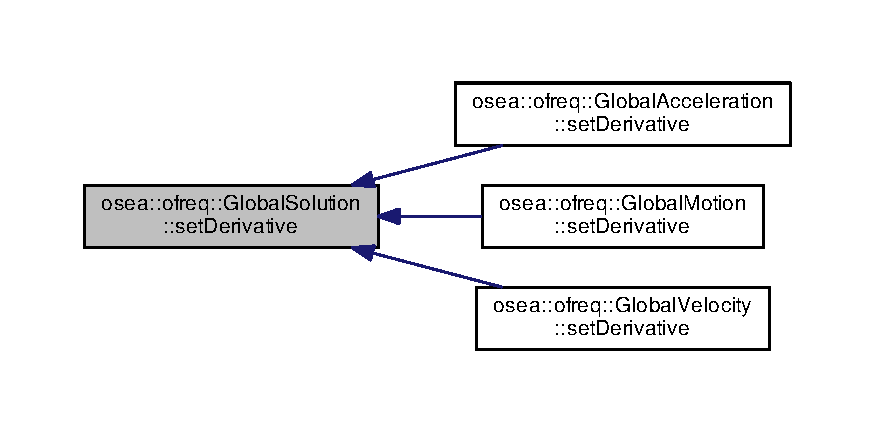
\includegraphics[width=350pt]{classosea_1_1ofreq_1_1_global_solution_a537163391f1f55d073720b20f69acfa5_icgraph}
\end{center}
\end{figure}




The documentation for this class was generated from the following files\-:\begin{DoxyCompactItemize}
\item 
globalsolution.\-h\item 
globalsolution.\-cpp\end{DoxyCompactItemize}

\hypertarget{classosea_1_1ofreq_1_1_global_velocity}{\section{osea\-:\-:ofreq\-:\-:Global\-Velocity Class Reference}
\label{classosea_1_1ofreq_1_1_global_velocity}\index{osea\-::ofreq\-::\-Global\-Velocity@{osea\-::ofreq\-::\-Global\-Velocity}}
}


{\ttfamily \#include $<$globalvelocity.\-h$>$}



Inheritance diagram for osea\-:\-:ofreq\-:\-:Global\-Velocity\-:
\nopagebreak
\begin{figure}[H]
\begin{center}
\leavevmode
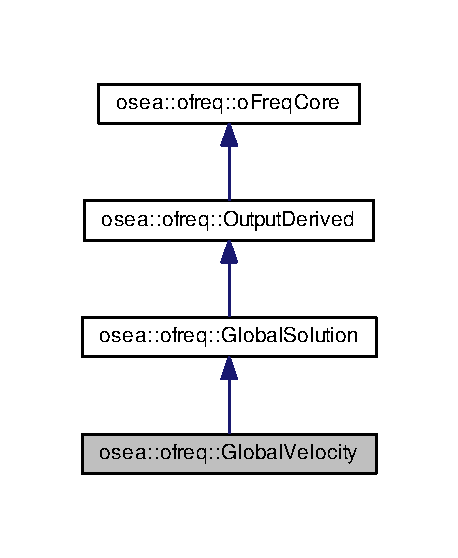
\includegraphics[height=550pt]{classosea_1_1ofreq_1_1_global_velocity__inherit__graph}
\end{center}
\end{figure}
\subsection*{Public Member Functions}
\begin{DoxyCompactItemize}
\item 
\hyperlink{classosea_1_1ofreq_1_1_global_velocity_a444ab39b351acd4e6ca7dc8088e2a9b8}{Global\-Velocity} ()
\item 
\hyperlink{classosea_1_1ofreq_1_1_global_velocity_a7992180d42ae3558cdcccfe56550ed94}{Global\-Velocity} (\hyperlink{classosea_1_1ofreq_1_1_outputs_body}{Outputs\-Body} $\ast$input)
\begin{DoxyCompactList}\small\item\em Constructor that also sets the pointer to the \hyperlink{classosea_1_1ofreq_1_1_outputs_body}{Outputs\-Body} object which contains the \hyperlink{classosea_1_1ofreq_1_1_output_derived}{Output\-Derived} object. \end{DoxyCompactList}\item 
\hyperlink{classosea_1_1ofreq_1_1_global_velocity_a2b8f719180b1786a582d90603db8f2d8}{$\sim$\-Global\-Velocity} ()
\item 
void \hyperlink{classosea_1_1ofreq_1_1_global_velocity_a11229a6dbc7f85f3c321b5eddb127f10}{set\-Derivative} (int ord)
\begin{DoxyCompactList}\small\item\em Sets the order of the derivative for the object. \end{DoxyCompactList}\end{DoxyCompactItemize}
\subsection*{Additional Inherited Members}


\subsection{Detailed Description}
This class represents the Global Velocity \hyperlink{classosea_1_1ofreq_1_1_solution}{Solution}. 

Definition at line 85 of file globalvelocity.\-h.



\subsection{Constructor \& Destructor Documentation}
\hypertarget{classosea_1_1ofreq_1_1_global_velocity_a444ab39b351acd4e6ca7dc8088e2a9b8}{\index{osea\-::ofreq\-::\-Global\-Velocity@{osea\-::ofreq\-::\-Global\-Velocity}!Global\-Velocity@{Global\-Velocity}}
\index{Global\-Velocity@{Global\-Velocity}!osea::ofreq::GlobalVelocity@{osea\-::ofreq\-::\-Global\-Velocity}}
\subsubsection[{Global\-Velocity}]{\setlength{\rightskip}{0pt plus 5cm}Global\-Velocity\-::\-Global\-Velocity (
\begin{DoxyParamCaption}
{}
\end{DoxyParamCaption}
)}}\label{classosea_1_1ofreq_1_1_global_velocity_a444ab39b351acd4e6ca7dc8088e2a9b8}
This default constructor creates a Global Velocity object. 

Definition at line 41 of file globalvelocity.\-cpp.

\hypertarget{classosea_1_1ofreq_1_1_global_velocity_a7992180d42ae3558cdcccfe56550ed94}{\index{osea\-::ofreq\-::\-Global\-Velocity@{osea\-::ofreq\-::\-Global\-Velocity}!Global\-Velocity@{Global\-Velocity}}
\index{Global\-Velocity@{Global\-Velocity}!osea::ofreq::GlobalVelocity@{osea\-::ofreq\-::\-Global\-Velocity}}
\subsubsection[{Global\-Velocity}]{\setlength{\rightskip}{0pt plus 5cm}Global\-Velocity\-::\-Global\-Velocity (
\begin{DoxyParamCaption}
\item[{{\bf Outputs\-Body} $\ast$}]{input}
\end{DoxyParamCaption}
)}}\label{classosea_1_1ofreq_1_1_global_velocity_a7992180d42ae3558cdcccfe56550ed94}


Constructor that also sets the pointer to the \hyperlink{classosea_1_1ofreq_1_1_outputs_body}{Outputs\-Body} object which contains the \hyperlink{classosea_1_1ofreq_1_1_output_derived}{Output\-Derived} object. 


\begin{DoxyParams}{Parameters}
{\em input} & Pointer to the \hyperlink{classosea_1_1ofreq_1_1_outputs_body}{Outputs\-Body} objec that contains this \hyperlink{classosea_1_1ofreq_1_1_output_derived}{Output\-Derived} object. Pointer passed by value.\\
\hline
\end{DoxyParams}
\begin{DoxySeeAlso}{See Also}
set\-Outputs\-Body() 
\end{DoxySeeAlso}


Definition at line 50 of file globalvelocity.\-cpp.

\hypertarget{classosea_1_1ofreq_1_1_global_velocity_a2b8f719180b1786a582d90603db8f2d8}{\index{osea\-::ofreq\-::\-Global\-Velocity@{osea\-::ofreq\-::\-Global\-Velocity}!$\sim$\-Global\-Velocity@{$\sim$\-Global\-Velocity}}
\index{$\sim$\-Global\-Velocity@{$\sim$\-Global\-Velocity}!osea::ofreq::GlobalVelocity@{osea\-::ofreq\-::\-Global\-Velocity}}
\subsubsection[{$\sim$\-Global\-Velocity}]{\setlength{\rightskip}{0pt plus 5cm}Global\-Velocity\-::$\sim$\-Global\-Velocity (
\begin{DoxyParamCaption}
{}
\end{DoxyParamCaption}
)}}\label{classosea_1_1ofreq_1_1_global_velocity_a2b8f719180b1786a582d90603db8f2d8}
The default destructor, nothing happens here. 

Definition at line 59 of file globalvelocity.\-cpp.



\subsection{Member Function Documentation}
\hypertarget{classosea_1_1ofreq_1_1_global_velocity_a11229a6dbc7f85f3c321b5eddb127f10}{\index{osea\-::ofreq\-::\-Global\-Velocity@{osea\-::ofreq\-::\-Global\-Velocity}!set\-Derivative@{set\-Derivative}}
\index{set\-Derivative@{set\-Derivative}!osea::ofreq::GlobalVelocity@{osea\-::ofreq\-::\-Global\-Velocity}}
\subsubsection[{set\-Derivative}]{\setlength{\rightskip}{0pt plus 5cm}void Global\-Velocity\-::set\-Derivative (
\begin{DoxyParamCaption}
\item[{int}]{ord}
\end{DoxyParamCaption}
)\hspace{0.3cm}{\ttfamily [virtual]}}}\label{classosea_1_1ofreq_1_1_global_velocity_a11229a6dbc7f85f3c321b5eddb127f10}


Sets the order of the derivative for the object. 


\begin{DoxyParams}{Parameters}
{\em ord} & Integer input that specifies the order of the derivative. Value can be anything from 0 or larger. Variable is passed by value. \\
\hline
\end{DoxyParams}


Reimplemented from \hyperlink{classosea_1_1ofreq_1_1_global_solution_a537163391f1f55d073720b20f69acfa5}{osea\-::ofreq\-::\-Global\-Solution}.



Definition at line 64 of file globalvelocity.\-cpp.



Here is the call graph for this function\-:
\nopagebreak
\begin{figure}[H]
\begin{center}
\leavevmode
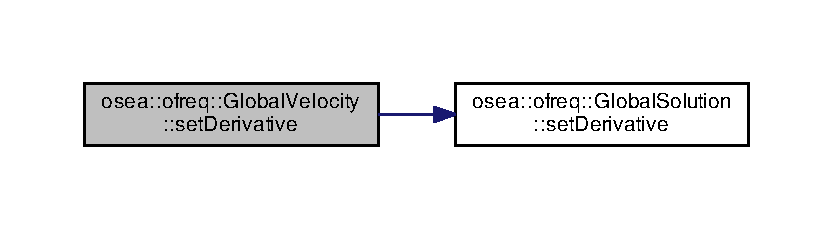
\includegraphics[width=350pt]{classosea_1_1ofreq_1_1_global_velocity_a11229a6dbc7f85f3c321b5eddb127f10_cgraph}
\end{center}
\end{figure}




The documentation for this class was generated from the following files\-:\begin{DoxyCompactItemize}
\item 
/home/\-Ship\-\_\-\-Design/\-Projects/\-D\-M\-S1305 Open\-S\-E\-A/master/200\-\_\-src/bin/ofreq/derived\-\_\-outputs/\hyperlink{globalvelocity_8h}{globalvelocity.\-h}\item 
/home/\-Ship\-\_\-\-Design/\-Projects/\-D\-M\-S1305 Open\-S\-E\-A/master/200\-\_\-src/bin/ofreq/derived\-\_\-outputs/\hyperlink{globalvelocity_8cpp}{globalvelocity.\-cpp}\end{DoxyCompactItemize}

\hypertarget{classosea_1_1ofreq_1_1mat_body}{\section{osea\-:\-:ofreq\-:\-:mat\-Body Class Reference}
\label{classosea_1_1ofreq_1_1mat_body}\index{osea\-::ofreq\-::mat\-Body@{osea\-::ofreq\-::mat\-Body}}
}


{\ttfamily \#include $<$matbody.\-h$>$}



Inheritance diagram for osea\-:\-:ofreq\-:\-:mat\-Body\-:\nopagebreak
\begin{figure}[H]
\begin{center}
\leavevmode
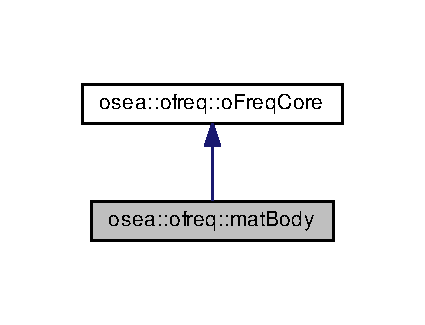
\includegraphics[width=204pt]{classosea_1_1ofreq_1_1mat_body__inherit__graph}
\end{center}
\end{figure}


Collaboration diagram for osea\-:\-:ofreq\-:\-:mat\-Body\-:\nopagebreak
\begin{figure}[H]
\begin{center}
\leavevmode
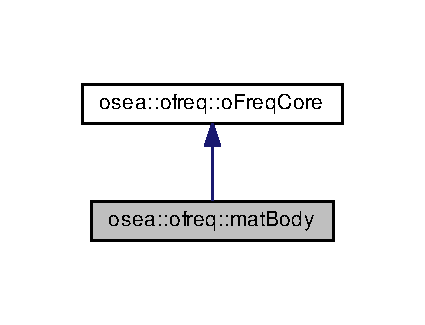
\includegraphics[width=204pt]{classosea_1_1ofreq_1_1mat_body__coll__graph}
\end{center}
\end{figure}
\subsection*{Public Member Functions}
\begin{DoxyCompactItemize}
\item 
\hyperlink{classosea_1_1ofreq_1_1mat_body_adbcb73fc9873660ca781493b2b2742a2}{mat\-Body} ()
\item 
\hyperlink{classosea_1_1ofreq_1_1mat_body_afcc3a6a87689dfbb5dfa72648a46c355}{$\sim$mat\-Body} ()
\item 
void \hyperlink{classosea_1_1ofreq_1_1mat_body_abb86318fbd7300ed01eae308551f9e96}{set\-Id} (int num)
\begin{DoxyCompactList}\small\item\em Sets the force id number for the object. \end{DoxyCompactList}\item 
int \hyperlink{classosea_1_1ofreq_1_1mat_body_a551183ad56eeba71ea4690574b1841e4}{get\-Id} ()
\begin{DoxyCompactList}\small\item\em Returns the force id number for the object. \end{DoxyCompactList}\item 
void \hyperlink{classosea_1_1ofreq_1_1mat_body_abb8ea32c84153da5dfc53d7b0dc836a5}{set\-Model\-Id} (int num)
\begin{DoxyCompactList}\small\item\em Sets the integer id of the motion model used by the \hyperlink{classosea_1_1ofreq_1_1mat_body}{mat\-Body} object. \end{DoxyCompactList}\item 
int \hyperlink{classosea_1_1ofreq_1_1mat_body_ae4c339b7ce6a93cf6e54bc998cbd5903}{get\-Model\-Id} ()
\begin{DoxyCompactList}\small\item\em Gets the integer id of the motion model used by the \hyperlink{classosea_1_1ofreq_1_1mat_body}{mat\-Body} object. \end{DoxyCompactList}\item 
arma\-::cx\-\_\-mat \& \hyperlink{classosea_1_1ofreq_1_1mat_body_a7c0b44be2aa75ae270168849c06e6067}{ref\-Mass} ()
\begin{DoxyCompactList}\small\item\em Returns a reference to the mass matrix. \end{DoxyCompactList}\item 
std\-::vector$<$ \hyperlink{classosea_1_1ofreq_1_1mat_force_react}{mat\-Force\-React} $>$ \& \hyperlink{classosea_1_1ofreq_1_1mat_body_aeb296f7c56b523b32ca12b58de56ef37}{list\-Force\-React\-\_\-user} ()
\begin{DoxyCompactList}\small\item\em Returns a reference to the Reactive \hyperlink{classosea_1_1ofreq_1_1_force}{Force}, user objects. \end{DoxyCompactList}\item 
\hyperlink{classosea_1_1ofreq_1_1mat_force_react}{mat\-Force\-React} \& \hyperlink{classosea_1_1ofreq_1_1mat_body_a53cbb789ae423084375b024954bf21f0}{list\-Force\-React\-\_\-user} (unsigned int index)
\begin{DoxyCompactList}\small\item\em Returns a reference to the Reactive \hyperlink{classosea_1_1ofreq_1_1_force}{Force}, user object specified by the index. \end{DoxyCompactList}\item 
std\-::vector$<$ \hyperlink{classosea_1_1ofreq_1_1mat_force_cross}{mat\-Force\-Cross} $>$ \& \hyperlink{classosea_1_1ofreq_1_1mat_body_a5dc37a8bb5143f2034ef6491969b2abe}{list\-Force\-Cross\-\_\-user} ()
\begin{DoxyCompactList}\small\item\em Returns a reference to the Cross-\/\-Body \hyperlink{classosea_1_1ofreq_1_1_force}{Force}, user objects. \end{DoxyCompactList}\item 
\hyperlink{classosea_1_1ofreq_1_1mat_force_cross}{mat\-Force\-Cross} \& \hyperlink{classosea_1_1ofreq_1_1mat_body_ae508a1904283a46d1fc5893da4080630}{list\-Force\-Cross\-\_\-user} (unsigned int index)
\begin{DoxyCompactList}\small\item\em Returns a reference to the Cross-\/\-Body \hyperlink{classosea_1_1ofreq_1_1_force}{Force}, user object specified by the index. \end{DoxyCompactList}\item 
std\-::vector$<$ \hyperlink{classosea_1_1ofreq_1_1mat_force_active}{mat\-Force\-Active} $>$ \& \hyperlink{classosea_1_1ofreq_1_1mat_body_a6a51e55baec56037eee824ec53af9b5d}{list\-Force\-Active\-\_\-user} ()
\begin{DoxyCompactList}\small\item\em Returns a reference to the Active \hyperlink{classosea_1_1ofreq_1_1_force}{Force}, user objects. \end{DoxyCompactList}\item 
\hyperlink{classosea_1_1ofreq_1_1mat_force_active}{mat\-Force\-Active} \& \hyperlink{classosea_1_1ofreq_1_1mat_body_a7d79de764dd75ad606a1cc9346b58676}{list\-Force\-Active\-\_\-user} (unsigned int index)
\begin{DoxyCompactList}\small\item\em Returns a reference to the Active \hyperlink{classosea_1_1ofreq_1_1_force}{Force}, user object specified by the index. \end{DoxyCompactList}\item 
std\-::vector$<$ \hyperlink{classosea_1_1ofreq_1_1mat_force_react}{mat\-Force\-React} $>$ \& \hyperlink{classosea_1_1ofreq_1_1mat_body_abead59c1604f4581a977e086874b2e7a}{list\-Force\-React\-\_\-hydro} ()
\begin{DoxyCompactList}\small\item\em Returns a reference to the Reactive \hyperlink{classosea_1_1ofreq_1_1_force}{Force}, hydro objects. \end{DoxyCompactList}\item 
\hyperlink{classosea_1_1ofreq_1_1mat_force_react}{mat\-Force\-React} \& \hyperlink{classosea_1_1ofreq_1_1mat_body_a052f37c59ad093d92e1155e0b300d1aa}{list\-Force\-React\-\_\-hydro} (unsigned int index)
\begin{DoxyCompactList}\small\item\em Returns a reference to the Reactive \hyperlink{classosea_1_1ofreq_1_1_force}{Force}, hydro object specified by the index. \end{DoxyCompactList}\item 
std\-::vector$<$ \hyperlink{classosea_1_1ofreq_1_1mat_force_cross}{mat\-Force\-Cross} $>$ \& \hyperlink{classosea_1_1ofreq_1_1mat_body_a40e3fc33bc7b1685b7f1400312f88f88}{list\-Force\-Cross\-\_\-hydro} ()
\begin{DoxyCompactList}\small\item\em Returns a reference to the Cross-\/\-Body \hyperlink{classosea_1_1ofreq_1_1_force}{Force}, hydro objects. \end{DoxyCompactList}\item 
\hyperlink{classosea_1_1ofreq_1_1mat_force_cross}{mat\-Force\-Cross} \& \hyperlink{classosea_1_1ofreq_1_1mat_body_ad8ce408c1042c080cda0d50a3864fa54}{list\-Force\-Cross\-\_\-hydro} (unsigned int index)
\begin{DoxyCompactList}\small\item\em Returns a reference to the Cross-\/\-Body \hyperlink{classosea_1_1ofreq_1_1_force}{Force}, hydro object specified by the index. \end{DoxyCompactList}\item 
std\-::vector$<$ \hyperlink{classosea_1_1ofreq_1_1mat_force_active}{mat\-Force\-Active} $>$ \& \hyperlink{classosea_1_1ofreq_1_1mat_body_a9733e23db05aac47a42cfca88fc9d679}{list\-Force\-Active\-\_\-hydro} ()
\begin{DoxyCompactList}\small\item\em Returns a reference to the Active \hyperlink{classosea_1_1ofreq_1_1_force}{Force}, hydro objects. \end{DoxyCompactList}\item 
\hyperlink{classosea_1_1ofreq_1_1mat_force_active}{mat\-Force\-Active} \& \hyperlink{classosea_1_1ofreq_1_1mat_body_aa1c0587dc82254db28ff71a9cc3261d7}{list\-Force\-Active\-\_\-hydro} (unsigned int index)
\begin{DoxyCompactList}\small\item\em Returns a reference to the Active \hyperlink{classosea_1_1ofreq_1_1_force}{Force}, hydro object specified by the index. \end{DoxyCompactList}\end{DoxyCompactItemize}
\subsection*{Additional Inherited Members}


\subsection{Detailed Description}
This class holds all data for a body and related force matrices. The \hyperlink{classosea_1_1ofreq_1_1mat_body}{mat\-Body} class contains data defined in a pure mathematical context. It is prepared for combination and solution. User interface items, such as relative coordinates and body names are stripped out. Definitions of equations, derivatives, and variables are replaced by sets of matrices. The body still contains force objects, but the objects are defined in terms of matrices. Each force object contains a vector of matrices, denoted by the derivative property. Each matrix within that vector represents a derivative, starting with order 0 (index 0 in the vector.) Each matrix is organized so that rows = equations, and columns = variables.

The class definition also includes a number and size property. The number denotes the body's position within a vector of bodies. The size denotes the number of equations used. This in turn notes how big the matrices must be to accomodate any forces from the body. 

\subsection{Constructor \& Destructor Documentation}
\hypertarget{classosea_1_1ofreq_1_1mat_body_adbcb73fc9873660ca781493b2b2742a2}{\index{osea\-::ofreq\-::mat\-Body@{osea\-::ofreq\-::mat\-Body}!mat\-Body@{mat\-Body}}
\index{mat\-Body@{mat\-Body}!osea::ofreq::matBody@{osea\-::ofreq\-::mat\-Body}}
\subsubsection[{mat\-Body}]{\setlength{\rightskip}{0pt plus 5cm}mat\-Body\-::mat\-Body (
\begin{DoxyParamCaption}
{}
\end{DoxyParamCaption}
)}}\label{classosea_1_1ofreq_1_1mat_body_adbcb73fc9873660ca781493b2b2742a2}
The default constructor. \hypertarget{classosea_1_1ofreq_1_1mat_body_afcc3a6a87689dfbb5dfa72648a46c355}{\index{osea\-::ofreq\-::mat\-Body@{osea\-::ofreq\-::mat\-Body}!$\sim$mat\-Body@{$\sim$mat\-Body}}
\index{$\sim$mat\-Body@{$\sim$mat\-Body}!osea::ofreq::matBody@{osea\-::ofreq\-::mat\-Body}}
\subsubsection[{$\sim$mat\-Body}]{\setlength{\rightskip}{0pt plus 5cm}mat\-Body\-::$\sim$mat\-Body (
\begin{DoxyParamCaption}
{}
\end{DoxyParamCaption}
)}}\label{classosea_1_1ofreq_1_1mat_body_afcc3a6a87689dfbb5dfa72648a46c355}
The default destructor, nothing happens here. 

\subsection{Member Function Documentation}
\hypertarget{classosea_1_1ofreq_1_1mat_body_a551183ad56eeba71ea4690574b1841e4}{\index{osea\-::ofreq\-::mat\-Body@{osea\-::ofreq\-::mat\-Body}!get\-Id@{get\-Id}}
\index{get\-Id@{get\-Id}!osea::ofreq::matBody@{osea\-::ofreq\-::mat\-Body}}
\subsubsection[{get\-Id}]{\setlength{\rightskip}{0pt plus 5cm}int mat\-Body\-::get\-Id (
\begin{DoxyParamCaption}
{}
\end{DoxyParamCaption}
)}}\label{classosea_1_1ofreq_1_1mat_body_a551183ad56eeba71ea4690574b1841e4}


Returns the force id number for the object. 

This is similar to the name parameter in other force objects. It is an identifier. In this case, a numerical identifier. Normally correlates to the objects index in a vector of other objects of the same class. \begin{DoxyReturn}{Returns}
Returns the force id number, integer data type. 
\end{DoxyReturn}


Here is the caller graph for this function\-:\nopagebreak
\begin{figure}[H]
\begin{center}
\leavevmode
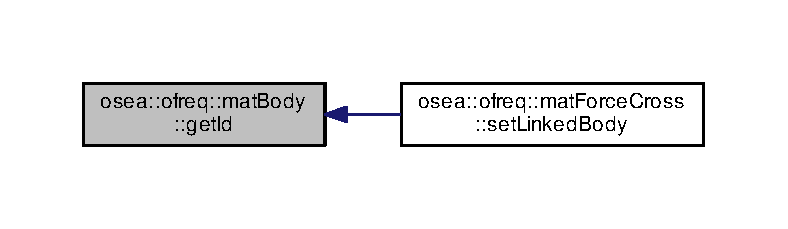
\includegraphics[width=350pt]{classosea_1_1ofreq_1_1mat_body_a551183ad56eeba71ea4690574b1841e4_icgraph}
\end{center}
\end{figure}


\hypertarget{classosea_1_1ofreq_1_1mat_body_ae4c339b7ce6a93cf6e54bc998cbd5903}{\index{osea\-::ofreq\-::mat\-Body@{osea\-::ofreq\-::mat\-Body}!get\-Model\-Id@{get\-Model\-Id}}
\index{get\-Model\-Id@{get\-Model\-Id}!osea::ofreq::matBody@{osea\-::ofreq\-::mat\-Body}}
\subsubsection[{get\-Model\-Id}]{\setlength{\rightskip}{0pt plus 5cm}int mat\-Body\-::get\-Model\-Id (
\begin{DoxyParamCaption}
{}
\end{DoxyParamCaption}
)}}\label{classosea_1_1ofreq_1_1mat_body_ae4c339b7ce6a93cf6e54bc998cbd5903}


Gets the integer id of the motion model used by the \hyperlink{classosea_1_1ofreq_1_1mat_body}{mat\-Body} object. 

Gets the integer id of the motion model used by the \hyperlink{classosea_1_1ofreq_1_1mat_body}{mat\-Body} object. \begin{DoxyReturn}{Returns}
Returns the integer id of the motion model used by the \hyperlink{classosea_1_1ofreq_1_1mat_body}{mat\-Body} object. Variable is passed by value. 
\end{DoxyReturn}
\hypertarget{classosea_1_1ofreq_1_1mat_body_a9733e23db05aac47a42cfca88fc9d679}{\index{osea\-::ofreq\-::mat\-Body@{osea\-::ofreq\-::mat\-Body}!list\-Force\-Active\-\_\-hydro@{list\-Force\-Active\-\_\-hydro}}
\index{list\-Force\-Active\-\_\-hydro@{list\-Force\-Active\-\_\-hydro}!osea::ofreq::matBody@{osea\-::ofreq\-::mat\-Body}}
\subsubsection[{list\-Force\-Active\-\_\-hydro}]{\setlength{\rightskip}{0pt plus 5cm}vector$<$ {\bf mat\-Force\-Active} $>$ \& mat\-Body\-::list\-Force\-Active\-\_\-hydro (
\begin{DoxyParamCaption}
{}
\end{DoxyParamCaption}
)}}\label{classosea_1_1ofreq_1_1mat_body_a9733e23db05aac47a42cfca88fc9d679}


Returns a reference to the Active \hyperlink{classosea_1_1ofreq_1_1_force}{Force}, hydro objects. 

Returns a reference to the Active \hyperlink{classosea_1_1ofreq_1_1_force}{Force}, hydro objects. This is a vector list of the Active \hyperlink{classosea_1_1ofreq_1_1_force}{Force} objects. Provides direct access to the variable and all the member functions of the vector class. \begin{DoxyReturn}{Returns}
This is a vector list of the Active \hyperlink{classosea_1_1ofreq_1_1_force}{Force} objects. Provides direct access to the variable and all the member functions of the vector class. Variable passed by reference. 
\end{DoxyReturn}
\hypertarget{classosea_1_1ofreq_1_1mat_body_aa1c0587dc82254db28ff71a9cc3261d7}{\index{osea\-::ofreq\-::mat\-Body@{osea\-::ofreq\-::mat\-Body}!list\-Force\-Active\-\_\-hydro@{list\-Force\-Active\-\_\-hydro}}
\index{list\-Force\-Active\-\_\-hydro@{list\-Force\-Active\-\_\-hydro}!osea::ofreq::matBody@{osea\-::ofreq\-::mat\-Body}}
\subsubsection[{list\-Force\-Active\-\_\-hydro}]{\setlength{\rightskip}{0pt plus 5cm}{\bf mat\-Force\-Active} \& mat\-Body\-::list\-Force\-Active\-\_\-hydro (
\begin{DoxyParamCaption}
\item[{unsigned int}]{index}
\end{DoxyParamCaption}
)}}\label{classosea_1_1ofreq_1_1mat_body_aa1c0587dc82254db28ff71a9cc3261d7}


Returns a reference to the Active \hyperlink{classosea_1_1ofreq_1_1_force}{Force}, hydro object specified by the index. 

This is a single item from the vector list of the Active \hyperlink{classosea_1_1ofreq_1_1_force}{Force} objects. Provides direct access to the variable. 
\begin{DoxyParams}{Parameters}
{\em index} & Unsigned integer. Index to specify which variable retrieve from the vector. \\
\hline
\end{DoxyParams}
\begin{DoxyReturn}{Returns}
Returns \hyperlink{classosea_1_1ofreq_1_1mat_force_active}{mat\-Force\-Active} object specified by index. Returned variable passed by reference. 
\end{DoxyReturn}
\begin{DoxySeeAlso}{See Also}
\hyperlink{classosea_1_1ofreq_1_1mat_force_active}{mat\-Force\-Active} 
\end{DoxySeeAlso}
\hypertarget{classosea_1_1ofreq_1_1mat_body_a6a51e55baec56037eee824ec53af9b5d}{\index{osea\-::ofreq\-::mat\-Body@{osea\-::ofreq\-::mat\-Body}!list\-Force\-Active\-\_\-user@{list\-Force\-Active\-\_\-user}}
\index{list\-Force\-Active\-\_\-user@{list\-Force\-Active\-\_\-user}!osea::ofreq::matBody@{osea\-::ofreq\-::mat\-Body}}
\subsubsection[{list\-Force\-Active\-\_\-user}]{\setlength{\rightskip}{0pt plus 5cm}vector$<$ {\bf mat\-Force\-Active} $>$ \& mat\-Body\-::list\-Force\-Active\-\_\-user (
\begin{DoxyParamCaption}
{}
\end{DoxyParamCaption}
)}}\label{classosea_1_1ofreq_1_1mat_body_a6a51e55baec56037eee824ec53af9b5d}


Returns a reference to the Active \hyperlink{classosea_1_1ofreq_1_1_force}{Force}, user objects. 

Returns a reference to the Active \hyperlink{classosea_1_1ofreq_1_1_force}{Force}, user objects. This is a vector list of the Active \hyperlink{classosea_1_1ofreq_1_1_force}{Force} objects. Provides direct access to the variable and all the member functions of the vector class. \begin{DoxyReturn}{Returns}
This is a vector list of the Active \hyperlink{classosea_1_1ofreq_1_1_force}{Force} objects. Provides direct access to the variable and all the member functions of the vector class. Variable passed by reference. 
\end{DoxyReturn}
\hypertarget{classosea_1_1ofreq_1_1mat_body_a7d79de764dd75ad606a1cc9346b58676}{\index{osea\-::ofreq\-::mat\-Body@{osea\-::ofreq\-::mat\-Body}!list\-Force\-Active\-\_\-user@{list\-Force\-Active\-\_\-user}}
\index{list\-Force\-Active\-\_\-user@{list\-Force\-Active\-\_\-user}!osea::ofreq::matBody@{osea\-::ofreq\-::mat\-Body}}
\subsubsection[{list\-Force\-Active\-\_\-user}]{\setlength{\rightskip}{0pt plus 5cm}{\bf mat\-Force\-Active} \& mat\-Body\-::list\-Force\-Active\-\_\-user (
\begin{DoxyParamCaption}
\item[{unsigned int}]{index}
\end{DoxyParamCaption}
)}}\label{classosea_1_1ofreq_1_1mat_body_a7d79de764dd75ad606a1cc9346b58676}


Returns a reference to the Active \hyperlink{classosea_1_1ofreq_1_1_force}{Force}, user object specified by the index. 

This is a single item from the vector list of the Active \hyperlink{classosea_1_1ofreq_1_1_force}{Force} objects. Provides direct access to the variable. 
\begin{DoxyParams}{Parameters}
{\em index} & Unsigned integer. Index to specify which variable retrieve from the vector. \\
\hline
\end{DoxyParams}
\begin{DoxyReturn}{Returns}
Returns \hyperlink{classosea_1_1ofreq_1_1mat_force_active}{mat\-Force\-Active} object specified by index. Returned variable passed by reference. 
\end{DoxyReturn}
\begin{DoxySeeAlso}{See Also}
\hyperlink{classosea_1_1ofreq_1_1mat_force_active}{mat\-Force\-Active} 
\end{DoxySeeAlso}
\hypertarget{classosea_1_1ofreq_1_1mat_body_a40e3fc33bc7b1685b7f1400312f88f88}{\index{osea\-::ofreq\-::mat\-Body@{osea\-::ofreq\-::mat\-Body}!list\-Force\-Cross\-\_\-hydro@{list\-Force\-Cross\-\_\-hydro}}
\index{list\-Force\-Cross\-\_\-hydro@{list\-Force\-Cross\-\_\-hydro}!osea::ofreq::matBody@{osea\-::ofreq\-::mat\-Body}}
\subsubsection[{list\-Force\-Cross\-\_\-hydro}]{\setlength{\rightskip}{0pt plus 5cm}vector$<$ {\bf mat\-Force\-Cross} $>$ \& mat\-Body\-::list\-Force\-Cross\-\_\-hydro (
\begin{DoxyParamCaption}
{}
\end{DoxyParamCaption}
)}}\label{classosea_1_1ofreq_1_1mat_body_a40e3fc33bc7b1685b7f1400312f88f88}


Returns a reference to the Cross-\/\-Body \hyperlink{classosea_1_1ofreq_1_1_force}{Force}, hydro objects. 

Returns a reference to the Cross-\/\-Body \hyperlink{classosea_1_1ofreq_1_1_force}{Force}, hydro objects. This is a vector list of the Cross-\/\-Body \hyperlink{classosea_1_1ofreq_1_1_force}{Force} objects. Provides direct access to the variable and all the member functions of the vector class. \begin{DoxyReturn}{Returns}
This is a vector list of the Cross-\/\-Body \hyperlink{classosea_1_1ofreq_1_1_force}{Force} objects. Provides direct access to the variable and all the member functions of the vector class. Variable passed by reference. 
\end{DoxyReturn}
\hypertarget{classosea_1_1ofreq_1_1mat_body_ad8ce408c1042c080cda0d50a3864fa54}{\index{osea\-::ofreq\-::mat\-Body@{osea\-::ofreq\-::mat\-Body}!list\-Force\-Cross\-\_\-hydro@{list\-Force\-Cross\-\_\-hydro}}
\index{list\-Force\-Cross\-\_\-hydro@{list\-Force\-Cross\-\_\-hydro}!osea::ofreq::matBody@{osea\-::ofreq\-::mat\-Body}}
\subsubsection[{list\-Force\-Cross\-\_\-hydro}]{\setlength{\rightskip}{0pt plus 5cm}{\bf mat\-Force\-Cross} \& mat\-Body\-::list\-Force\-Cross\-\_\-hydro (
\begin{DoxyParamCaption}
\item[{unsigned int}]{index}
\end{DoxyParamCaption}
)}}\label{classosea_1_1ofreq_1_1mat_body_ad8ce408c1042c080cda0d50a3864fa54}


Returns a reference to the Cross-\/\-Body \hyperlink{classosea_1_1ofreq_1_1_force}{Force}, hydro object specified by the index. 

This is a single item from the vector list of the Cross-\/\-Body \hyperlink{classosea_1_1ofreq_1_1_force}{Force} objects. Provides direct access to the variable. 
\begin{DoxyParams}{Parameters}
{\em index} & Unsigned integer. Index to specify which variable retrieve from the vector. \\
\hline
\end{DoxyParams}
\begin{DoxyReturn}{Returns}
Returns \hyperlink{classosea_1_1ofreq_1_1mat_force_cross}{mat\-Force\-Cross} object specified by index. Returned variable passed by reference. 
\end{DoxyReturn}
\begin{DoxySeeAlso}{See Also}
\hyperlink{classosea_1_1ofreq_1_1mat_force_cross}{mat\-Force\-Cross} 
\end{DoxySeeAlso}
\hypertarget{classosea_1_1ofreq_1_1mat_body_a5dc37a8bb5143f2034ef6491969b2abe}{\index{osea\-::ofreq\-::mat\-Body@{osea\-::ofreq\-::mat\-Body}!list\-Force\-Cross\-\_\-user@{list\-Force\-Cross\-\_\-user}}
\index{list\-Force\-Cross\-\_\-user@{list\-Force\-Cross\-\_\-user}!osea::ofreq::matBody@{osea\-::ofreq\-::mat\-Body}}
\subsubsection[{list\-Force\-Cross\-\_\-user}]{\setlength{\rightskip}{0pt plus 5cm}vector$<$ {\bf mat\-Force\-Cross} $>$ \& mat\-Body\-::list\-Force\-Cross\-\_\-user (
\begin{DoxyParamCaption}
{}
\end{DoxyParamCaption}
)}}\label{classosea_1_1ofreq_1_1mat_body_a5dc37a8bb5143f2034ef6491969b2abe}


Returns a reference to the Cross-\/\-Body \hyperlink{classosea_1_1ofreq_1_1_force}{Force}, user objects. 

Returns a reference to the Cross-\/\-Body \hyperlink{classosea_1_1ofreq_1_1_force}{Force}, user objects. This is a vector list of the Cross-\/\-Body \hyperlink{classosea_1_1ofreq_1_1_force}{Force} objects. Provides direct access to the variable and all the member functions of the vector class. \begin{DoxyReturn}{Returns}
This is a vector list of the Cross-\/\-Body \hyperlink{classosea_1_1ofreq_1_1_force}{Force} objects. Provides direct access to the variable and all the member functions of the vector class. Variable passed by reference. 
\end{DoxyReturn}
\hypertarget{classosea_1_1ofreq_1_1mat_body_ae508a1904283a46d1fc5893da4080630}{\index{osea\-::ofreq\-::mat\-Body@{osea\-::ofreq\-::mat\-Body}!list\-Force\-Cross\-\_\-user@{list\-Force\-Cross\-\_\-user}}
\index{list\-Force\-Cross\-\_\-user@{list\-Force\-Cross\-\_\-user}!osea::ofreq::matBody@{osea\-::ofreq\-::mat\-Body}}
\subsubsection[{list\-Force\-Cross\-\_\-user}]{\setlength{\rightskip}{0pt plus 5cm}{\bf mat\-Force\-Cross} \& mat\-Body\-::list\-Force\-Cross\-\_\-user (
\begin{DoxyParamCaption}
\item[{unsigned int}]{index}
\end{DoxyParamCaption}
)}}\label{classosea_1_1ofreq_1_1mat_body_ae508a1904283a46d1fc5893da4080630}


Returns a reference to the Cross-\/\-Body \hyperlink{classosea_1_1ofreq_1_1_force}{Force}, user object specified by the index. 

This is a single item from the vector list of the Cross-\/\-Body \hyperlink{classosea_1_1ofreq_1_1_force}{Force} objects. Provides direct access to the variable. 
\begin{DoxyParams}{Parameters}
{\em index} & Unsigned integer. Index to specify which variable retrieve from the vector. \\
\hline
\end{DoxyParams}
\begin{DoxyReturn}{Returns}
Returns \hyperlink{classosea_1_1ofreq_1_1mat_force_cross}{mat\-Force\-Cross} object specified by index. Returned variable passed by reference. 
\end{DoxyReturn}
\begin{DoxySeeAlso}{See Also}
\hyperlink{classosea_1_1ofreq_1_1mat_force_cross}{mat\-Force\-Cross} 
\end{DoxySeeAlso}
\hypertarget{classosea_1_1ofreq_1_1mat_body_abead59c1604f4581a977e086874b2e7a}{\index{osea\-::ofreq\-::mat\-Body@{osea\-::ofreq\-::mat\-Body}!list\-Force\-React\-\_\-hydro@{list\-Force\-React\-\_\-hydro}}
\index{list\-Force\-React\-\_\-hydro@{list\-Force\-React\-\_\-hydro}!osea::ofreq::matBody@{osea\-::ofreq\-::mat\-Body}}
\subsubsection[{list\-Force\-React\-\_\-hydro}]{\setlength{\rightskip}{0pt plus 5cm}vector$<$ {\bf mat\-Force\-React} $>$ \& mat\-Body\-::list\-Force\-React\-\_\-hydro (
\begin{DoxyParamCaption}
{}
\end{DoxyParamCaption}
)}}\label{classosea_1_1ofreq_1_1mat_body_abead59c1604f4581a977e086874b2e7a}


Returns a reference to the Reactive \hyperlink{classosea_1_1ofreq_1_1_force}{Force}, hydro objects. 

Returns a reference to the Reactive \hyperlink{classosea_1_1ofreq_1_1_force}{Force}, hydro objects. This is a vector list of the Reactive \hyperlink{classosea_1_1ofreq_1_1_force}{Force} objects. Provides direct access to the variable and all the member functions of the vector class. \begin{DoxyReturn}{Returns}
This is a vector list of the Reactive \hyperlink{classosea_1_1ofreq_1_1_force}{Force} objects. Provides direct access to the variable and all the member functions of the vector class. Variable passed by reference. 
\end{DoxyReturn}
\hypertarget{classosea_1_1ofreq_1_1mat_body_a052f37c59ad093d92e1155e0b300d1aa}{\index{osea\-::ofreq\-::mat\-Body@{osea\-::ofreq\-::mat\-Body}!list\-Force\-React\-\_\-hydro@{list\-Force\-React\-\_\-hydro}}
\index{list\-Force\-React\-\_\-hydro@{list\-Force\-React\-\_\-hydro}!osea::ofreq::matBody@{osea\-::ofreq\-::mat\-Body}}
\subsubsection[{list\-Force\-React\-\_\-hydro}]{\setlength{\rightskip}{0pt plus 5cm}{\bf mat\-Force\-React} \& mat\-Body\-::list\-Force\-React\-\_\-hydro (
\begin{DoxyParamCaption}
\item[{unsigned int}]{index}
\end{DoxyParamCaption}
)}}\label{classosea_1_1ofreq_1_1mat_body_a052f37c59ad093d92e1155e0b300d1aa}


Returns a reference to the Reactive \hyperlink{classosea_1_1ofreq_1_1_force}{Force}, hydro object specified by the index. 

This is a single item from the vector list of the Reactive \hyperlink{classosea_1_1ofreq_1_1_force}{Force} objects. Provides direct access to the variable. 
\begin{DoxyParams}{Parameters}
{\em index} & Unsigned integer. Index to specify which variable retrieve from the vector. \\
\hline
\end{DoxyParams}
\begin{DoxyReturn}{Returns}
Returns \hyperlink{classosea_1_1ofreq_1_1mat_force_react}{mat\-Force\-React} object specified by index. Returned variable passed by reference. 
\end{DoxyReturn}
\begin{DoxySeeAlso}{See Also}
\hyperlink{classosea_1_1ofreq_1_1mat_force_react}{mat\-Force\-React} 
\end{DoxySeeAlso}
\hypertarget{classosea_1_1ofreq_1_1mat_body_aeb296f7c56b523b32ca12b58de56ef37}{\index{osea\-::ofreq\-::mat\-Body@{osea\-::ofreq\-::mat\-Body}!list\-Force\-React\-\_\-user@{list\-Force\-React\-\_\-user}}
\index{list\-Force\-React\-\_\-user@{list\-Force\-React\-\_\-user}!osea::ofreq::matBody@{osea\-::ofreq\-::mat\-Body}}
\subsubsection[{list\-Force\-React\-\_\-user}]{\setlength{\rightskip}{0pt plus 5cm}vector$<$ {\bf mat\-Force\-React} $>$ \& mat\-Body\-::list\-Force\-React\-\_\-user (
\begin{DoxyParamCaption}
{}
\end{DoxyParamCaption}
)}}\label{classosea_1_1ofreq_1_1mat_body_aeb296f7c56b523b32ca12b58de56ef37}


Returns a reference to the Reactive \hyperlink{classosea_1_1ofreq_1_1_force}{Force}, user objects. 

Returns a reference to the Reactive \hyperlink{classosea_1_1ofreq_1_1_force}{Force}, user objects. This is a vector list of the Reactive \hyperlink{classosea_1_1ofreq_1_1_force}{Force} objects. Provides direct access to the variable and all the member functions of the vector class. \begin{DoxyReturn}{Returns}
This is a vector list of the Reactive \hyperlink{classosea_1_1ofreq_1_1_force}{Force} objects. Provides direct access to the variable and all the member functions of the vector class. Variable passed by reference. 
\end{DoxyReturn}
\hypertarget{classosea_1_1ofreq_1_1mat_body_a53cbb789ae423084375b024954bf21f0}{\index{osea\-::ofreq\-::mat\-Body@{osea\-::ofreq\-::mat\-Body}!list\-Force\-React\-\_\-user@{list\-Force\-React\-\_\-user}}
\index{list\-Force\-React\-\_\-user@{list\-Force\-React\-\_\-user}!osea::ofreq::matBody@{osea\-::ofreq\-::mat\-Body}}
\subsubsection[{list\-Force\-React\-\_\-user}]{\setlength{\rightskip}{0pt plus 5cm}{\bf mat\-Force\-React} \& mat\-Body\-::list\-Force\-React\-\_\-user (
\begin{DoxyParamCaption}
\item[{unsigned int}]{index}
\end{DoxyParamCaption}
)}}\label{classosea_1_1ofreq_1_1mat_body_a53cbb789ae423084375b024954bf21f0}


Returns a reference to the Reactive \hyperlink{classosea_1_1ofreq_1_1_force}{Force}, user object specified by the index. 

This is a single item from the vector list of the Reactive \hyperlink{classosea_1_1ofreq_1_1_force}{Force} objects. Provides direct access to the variable. 
\begin{DoxyParams}{Parameters}
{\em index} & Unsigned integer. Index to specify which variable retrieve from the vector. \\
\hline
\end{DoxyParams}
\begin{DoxyReturn}{Returns}
Returns \hyperlink{classosea_1_1ofreq_1_1mat_force_react}{mat\-Force\-React} object specified by index. Returned variable passed by reference. 
\end{DoxyReturn}
\begin{DoxySeeAlso}{See Also}
\hyperlink{classosea_1_1ofreq_1_1mat_force_react}{mat\-Force\-React} 
\end{DoxySeeAlso}
\hypertarget{classosea_1_1ofreq_1_1mat_body_a7c0b44be2aa75ae270168849c06e6067}{\index{osea\-::ofreq\-::mat\-Body@{osea\-::ofreq\-::mat\-Body}!ref\-Mass@{ref\-Mass}}
\index{ref\-Mass@{ref\-Mass}!osea::ofreq::matBody@{osea\-::ofreq\-::mat\-Body}}
\subsubsection[{ref\-Mass}]{\setlength{\rightskip}{0pt plus 5cm}cx\-\_\-mat \& mat\-Body\-::ref\-Mass (
\begin{DoxyParamCaption}
{}
\end{DoxyParamCaption}
)}}\label{classosea_1_1ofreq_1_1mat_body_a7c0b44be2aa75ae270168849c06e6067}


Returns a reference to the mass matrix. 

Returns a reference to the mass matrix. \begin{DoxyReturn}{Returns}
Returns a reference to the mass matrix. Variable passed by reference. 
\end{DoxyReturn}
\hypertarget{classosea_1_1ofreq_1_1mat_body_abb86318fbd7300ed01eae308551f9e96}{\index{osea\-::ofreq\-::mat\-Body@{osea\-::ofreq\-::mat\-Body}!set\-Id@{set\-Id}}
\index{set\-Id@{set\-Id}!osea::ofreq::matBody@{osea\-::ofreq\-::mat\-Body}}
\subsubsection[{set\-Id}]{\setlength{\rightskip}{0pt plus 5cm}void mat\-Body\-::set\-Id (
\begin{DoxyParamCaption}
\item[{int}]{num}
\end{DoxyParamCaption}
)}}\label{classosea_1_1ofreq_1_1mat_body_abb86318fbd7300ed01eae308551f9e96}


Sets the force id number for the object. 

This is similar to the name parameter in other force objects. It is an identifier. In this case, a numerical identifier. Normally correlates to the objects index in a vector of other objects of the same class. 
\begin{DoxyParams}{Parameters}
{\em num} & The integer number to input as the objects integer id. \\
\hline
\end{DoxyParams}
\hypertarget{classosea_1_1ofreq_1_1mat_body_abb8ea32c84153da5dfc53d7b0dc836a5}{\index{osea\-::ofreq\-::mat\-Body@{osea\-::ofreq\-::mat\-Body}!set\-Model\-Id@{set\-Model\-Id}}
\index{set\-Model\-Id@{set\-Model\-Id}!osea::ofreq::matBody@{osea\-::ofreq\-::mat\-Body}}
\subsubsection[{set\-Model\-Id}]{\setlength{\rightskip}{0pt plus 5cm}void mat\-Body\-::set\-Model\-Id (
\begin{DoxyParamCaption}
\item[{int}]{num}
\end{DoxyParamCaption}
)}}\label{classosea_1_1ofreq_1_1mat_body_abb8ea32c84153da5dfc53d7b0dc836a5}


Sets the integer id of the motion model used by the \hyperlink{classosea_1_1ofreq_1_1mat_body}{mat\-Body} object. 

Sets the integer id of the motion model used by the \hyperlink{classosea_1_1ofreq_1_1mat_body}{mat\-Body} object. 
\begin{DoxyParams}{Parameters}
{\em num} & Integer. The integer id of the motion model used by the \hyperlink{classosea_1_1ofreq_1_1mat_body}{mat\-Body} object. Variable is passed by value. \\
\hline
\end{DoxyParams}


The documentation for this class was generated from the following files\-:\begin{DoxyCompactItemize}
\item 
matbody.\-h\item 
matbody.\-cpp\end{DoxyCompactItemize}

\hypertarget{classosea_1_1ofreq_1_1mat_force_active}{\section{osea\-:\-:ofreq\-:\-:mat\-Force\-Active Class Reference}
\label{classosea_1_1ofreq_1_1mat_force_active}\index{osea\-::ofreq\-::mat\-Force\-Active@{osea\-::ofreq\-::mat\-Force\-Active}}
}


{\ttfamily \#include $<$matforceactive.\-h$>$}



Inheritance diagram for osea\-:\-:ofreq\-:\-:mat\-Force\-Active\-:\nopagebreak
\begin{figure}[H]
\begin{center}
\leavevmode
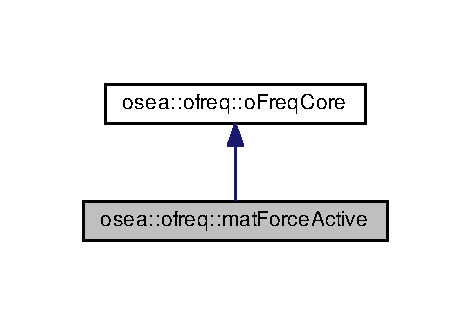
\includegraphics[width=226pt]{classosea_1_1ofreq_1_1mat_force_active__inherit__graph}
\end{center}
\end{figure}


Collaboration diagram for osea\-:\-:ofreq\-:\-:mat\-Force\-Active\-:\nopagebreak
\begin{figure}[H]
\begin{center}
\leavevmode
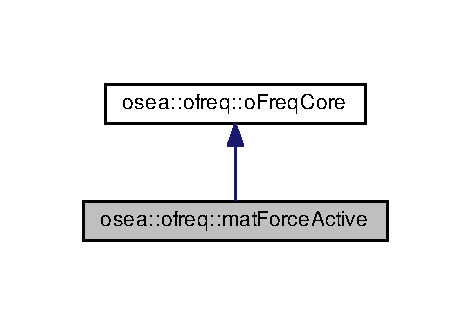
\includegraphics[width=226pt]{classosea_1_1ofreq_1_1mat_force_active__coll__graph}
\end{center}
\end{figure}
\subsection*{Public Member Functions}
\begin{DoxyCompactItemize}
\item 
\hyperlink{classosea_1_1ofreq_1_1mat_force_active_addc507c90f98f3a9bb9bfe57897df3ca}{mat\-Force\-Active} ()
\item 
\hyperlink{classosea_1_1ofreq_1_1mat_force_active_aba1957829e2109f03c6fc03990258210}{$\sim$mat\-Force\-Active} ()
\item 
\hypertarget{classosea_1_1ofreq_1_1mat_force_active_a8bc32fc773bd6c29d8bd7790194a10cf}{\hyperlink{classosea_1_1ofreq_1_1mat_force_active}{mat\-Force\-Active} {\bfseries operator+} (\hyperlink{classosea_1_1ofreq_1_1mat_force_active}{mat\-Force\-Active} \&force\-Other)}\label{classosea_1_1ofreq_1_1mat_force_active_a8bc32fc773bd6c29d8bd7790194a10cf}

\item 
\hypertarget{classosea_1_1ofreq_1_1mat_force_active_a150bda87debf622dacb439e8e983fa3c}{\hyperlink{classosea_1_1ofreq_1_1mat_force_active}{mat\-Force\-Active} {\bfseries operator-\/} (\hyperlink{classosea_1_1ofreq_1_1mat_force_active}{mat\-Force\-Active} \&force\-Other)}\label{classosea_1_1ofreq_1_1mat_force_active_a150bda87debf622dacb439e8e983fa3c}

\item 
arma\-::cx\-\_\-mat \& \hyperlink{classosea_1_1ofreq_1_1mat_force_active_ab2cb4bbd11161f8c2944675815dea81c}{list\-Coefficient} ()
\begin{DoxyCompactList}\small\item\em Returns the coefficients matrix. \end{DoxyCompactList}\item 
void \hyperlink{classosea_1_1ofreq_1_1mat_force_active_a2784051c78388741bf1cf66d18df0b2c}{set\-Id} (int num)
\begin{DoxyCompactList}\small\item\em Sets the force id number for the object. \end{DoxyCompactList}\item 
int \hyperlink{classosea_1_1ofreq_1_1mat_force_active_a48a33b65af2085268a2f03fb212a39d3}{get\-Id} ()
\begin{DoxyCompactList}\small\item\em Returns the force id number for the object. \end{DoxyCompactList}\item 
int \hyperlink{classosea_1_1ofreq_1_1mat_force_active_aa17a21eb9a9ea9e1a36fae4dbc2b09bf}{get\-Mat\-Size} ()
\begin{DoxyCompactList}\small\item\em Returns the size of the matrix in each order of derivative. \end{DoxyCompactList}\end{DoxyCompactItemize}
\subsection*{Additional Inherited Members}


\subsection{Detailed Description}
This class holds all data for an active force matrix. 

\subsection{Constructor \& Destructor Documentation}
\hypertarget{classosea_1_1ofreq_1_1mat_force_active_addc507c90f98f3a9bb9bfe57897df3ca}{\index{osea\-::ofreq\-::mat\-Force\-Active@{osea\-::ofreq\-::mat\-Force\-Active}!mat\-Force\-Active@{mat\-Force\-Active}}
\index{mat\-Force\-Active@{mat\-Force\-Active}!osea::ofreq::matForceActive@{osea\-::ofreq\-::mat\-Force\-Active}}
\subsubsection[{mat\-Force\-Active}]{\setlength{\rightskip}{0pt plus 5cm}mat\-Force\-Active\-::mat\-Force\-Active (
\begin{DoxyParamCaption}
{}
\end{DoxyParamCaption}
)}}\label{classosea_1_1ofreq_1_1mat_force_active_addc507c90f98f3a9bb9bfe57897df3ca}
The default constructor. \hypertarget{classosea_1_1ofreq_1_1mat_force_active_aba1957829e2109f03c6fc03990258210}{\index{osea\-::ofreq\-::mat\-Force\-Active@{osea\-::ofreq\-::mat\-Force\-Active}!$\sim$mat\-Force\-Active@{$\sim$mat\-Force\-Active}}
\index{$\sim$mat\-Force\-Active@{$\sim$mat\-Force\-Active}!osea::ofreq::matForceActive@{osea\-::ofreq\-::mat\-Force\-Active}}
\subsubsection[{$\sim$mat\-Force\-Active}]{\setlength{\rightskip}{0pt plus 5cm}mat\-Force\-Active\-::$\sim$mat\-Force\-Active (
\begin{DoxyParamCaption}
{}
\end{DoxyParamCaption}
)}}\label{classosea_1_1ofreq_1_1mat_force_active_aba1957829e2109f03c6fc03990258210}
The default destructor, nothing happens here. 

\subsection{Member Function Documentation}
\hypertarget{classosea_1_1ofreq_1_1mat_force_active_a48a33b65af2085268a2f03fb212a39d3}{\index{osea\-::ofreq\-::mat\-Force\-Active@{osea\-::ofreq\-::mat\-Force\-Active}!get\-Id@{get\-Id}}
\index{get\-Id@{get\-Id}!osea::ofreq::matForceActive@{osea\-::ofreq\-::mat\-Force\-Active}}
\subsubsection[{get\-Id}]{\setlength{\rightskip}{0pt plus 5cm}int mat\-Force\-Active\-::get\-Id (
\begin{DoxyParamCaption}
{}
\end{DoxyParamCaption}
)}}\label{classosea_1_1ofreq_1_1mat_force_active_a48a33b65af2085268a2f03fb212a39d3}


Returns the force id number for the object. 

This is similar to the name parameter in other force objects. It is an identifier. In this case, a numerical identifier. Normally correlates to the objects index in a vector of other objects of the same class. \begin{DoxyReturn}{Returns}
Returns the force id number, integer data type. 
\end{DoxyReturn}
\hypertarget{classosea_1_1ofreq_1_1mat_force_active_aa17a21eb9a9ea9e1a36fae4dbc2b09bf}{\index{osea\-::ofreq\-::mat\-Force\-Active@{osea\-::ofreq\-::mat\-Force\-Active}!get\-Mat\-Size@{get\-Mat\-Size}}
\index{get\-Mat\-Size@{get\-Mat\-Size}!osea::ofreq::matForceActive@{osea\-::ofreq\-::mat\-Force\-Active}}
\subsubsection[{get\-Mat\-Size}]{\setlength{\rightskip}{0pt plus 5cm}int mat\-Force\-Active\-::get\-Mat\-Size (
\begin{DoxyParamCaption}
{}
\end{DoxyParamCaption}
)}}\label{classosea_1_1ofreq_1_1mat_force_active_aa17a21eb9a9ea9e1a36fae4dbc2b09bf}


Returns the size of the matrix in each order of derivative. 

Returns the size of the matrix in each order of derivative. Integer output type. \begin{DoxyReturn}{Returns}
Returns the size of the matrix in each order of derivative. 
\end{DoxyReturn}
\hypertarget{classosea_1_1ofreq_1_1mat_force_active_ab2cb4bbd11161f8c2944675815dea81c}{\index{osea\-::ofreq\-::mat\-Force\-Active@{osea\-::ofreq\-::mat\-Force\-Active}!list\-Coefficient@{list\-Coefficient}}
\index{list\-Coefficient@{list\-Coefficient}!osea::ofreq::matForceActive@{osea\-::ofreq\-::mat\-Force\-Active}}
\subsubsection[{list\-Coefficient}]{\setlength{\rightskip}{0pt plus 5cm}cx\-\_\-mat \& mat\-Force\-Active\-::list\-Coefficient (
\begin{DoxyParamCaption}
{}
\end{DoxyParamCaption}
)}}\label{classosea_1_1ofreq_1_1mat_force_active_ab2cb4bbd11161f8c2944675815dea81c}


Returns the coefficients matrix. 

Returns the coefficients matrix. \begin{DoxyReturn}{Returns}
Returns the coefficients matrix. 
\end{DoxyReturn}


Here is the caller graph for this function\-:
\nopagebreak
\begin{figure}[H]
\begin{center}
\leavevmode
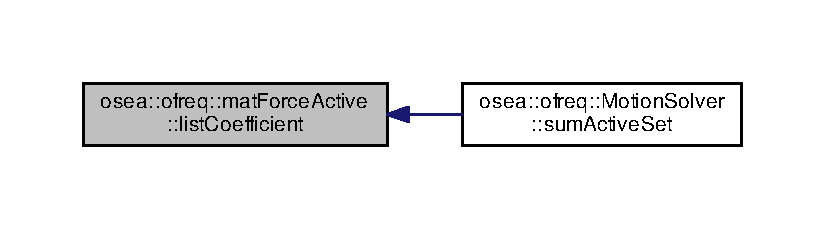
\includegraphics[width=350pt]{classosea_1_1ofreq_1_1mat_force_active_ab2cb4bbd11161f8c2944675815dea81c_icgraph}
\end{center}
\end{figure}


\hypertarget{classosea_1_1ofreq_1_1mat_force_active_a2784051c78388741bf1cf66d18df0b2c}{\index{osea\-::ofreq\-::mat\-Force\-Active@{osea\-::ofreq\-::mat\-Force\-Active}!set\-Id@{set\-Id}}
\index{set\-Id@{set\-Id}!osea::ofreq::matForceActive@{osea\-::ofreq\-::mat\-Force\-Active}}
\subsubsection[{set\-Id}]{\setlength{\rightskip}{0pt plus 5cm}void mat\-Force\-Active\-::set\-Id (
\begin{DoxyParamCaption}
\item[{int}]{num}
\end{DoxyParamCaption}
)}}\label{classosea_1_1ofreq_1_1mat_force_active_a2784051c78388741bf1cf66d18df0b2c}


Sets the force id number for the object. 

This is similar to the name parameter in other force objects. It is an identifier. In this case, a numerical identifier. Normally correlates to the objects index in a vector of other objects of the same class. 
\begin{DoxyParams}{Parameters}
{\em num} & The integer number to input as the objects integer id. \\
\hline
\end{DoxyParams}


The documentation for this class was generated from the following files\-:\begin{DoxyCompactItemize}
\item 
matforceactive.\-h\item 
matforceactive.\-cpp\end{DoxyCompactItemize}

\hypertarget{classosea_1_1ofreq_1_1mat_force_cross}{\section{osea\-:\-:ofreq\-:\-:mat\-Force\-Cross Class Reference}
\label{classosea_1_1ofreq_1_1mat_force_cross}\index{osea\-::ofreq\-::mat\-Force\-Cross@{osea\-::ofreq\-::mat\-Force\-Cross}}
}


{\ttfamily \#include $<$matforcecross.\-h$>$}



Inheritance diagram for osea\-:\-:ofreq\-:\-:mat\-Force\-Cross\-:
\nopagebreak
\begin{figure}[H]
\begin{center}
\leavevmode
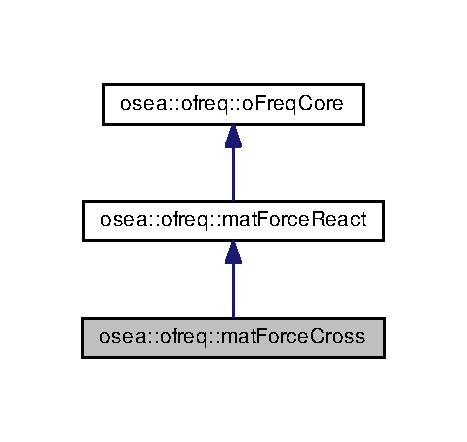
\includegraphics[width=242pt]{classosea_1_1ofreq_1_1mat_force_cross__inherit__graph}
\end{center}
\end{figure}
\subsection*{Public Member Functions}
\begin{DoxyCompactItemize}
\item 
\hyperlink{classosea_1_1ofreq_1_1mat_force_cross_a8ceccb692bece20135f104f2f78dcf20}{mat\-Force\-Cross} ()
\item 
\hyperlink{classosea_1_1ofreq_1_1mat_force_cross_a7887135f4a9ee649d161ca5ca649675f}{mat\-Force\-Cross} (std\-::vector$<$ arma\-::cx\-\_\-mat $>$ force\-In)
\begin{DoxyCompactList}\small\item\em The constructor. Takes a vector of complex matrices and stores them as derivatives. \end{DoxyCompactList}\item 
\hyperlink{classosea_1_1ofreq_1_1mat_force_cross_a2eb0a76db0d4f994287d8368699bb036}{$\sim$mat\-Force\-Cross} ()
\item 
\hyperlink{classosea_1_1ofreq_1_1mat_force_cross}{mat\-Force\-Cross} \hyperlink{classosea_1_1ofreq_1_1mat_force_cross_a9cb8a17edf38bebb728ff47261175614}{operator+} (\hyperlink{classosea_1_1ofreq_1_1mat_force_cross}{mat\-Force\-Cross} \&force\-Other)
\begin{DoxyCompactList}\small\item\em Operator overload to add two \hyperlink{classosea_1_1ofreq_1_1mat_force_cross}{mat\-Force\-Cross} objects together. \end{DoxyCompactList}\item 
\hyperlink{classosea_1_1ofreq_1_1mat_force_cross}{mat\-Force\-Cross} \hyperlink{classosea_1_1ofreq_1_1mat_force_cross_af22b49c1536dc753f99b34a3eba1c8e7}{operator-\/} (\hyperlink{classosea_1_1ofreq_1_1mat_force_cross}{mat\-Force\-Cross} \&force\-Other)
\begin{DoxyCompactList}\small\item\em Operator overload to subtract two \hyperlink{classosea_1_1ofreq_1_1mat_force_cross}{mat\-Force\-Cross} objects together. \end{DoxyCompactList}\item 
void \hyperlink{classosea_1_1ofreq_1_1mat_force_cross_a546ca085994682e1e8160ce3014ffaae}{set\-Linked\-Body} (\hyperlink{classosea_1_1ofreq_1_1mat_body}{mat\-Body} \&Bod\-In)
\item 
\hyperlink{classosea_1_1ofreq_1_1mat_body}{mat\-Body} $\ast$ \hyperlink{classosea_1_1ofreq_1_1mat_force_cross_a240be184a1a56ac5541ea0acfbcb9ec5}{get\-Linked\-Body} ()
\item 
void \hyperlink{classosea_1_1ofreq_1_1mat_force_cross_a285c83c27df6413f90665480d2f3a4ed}{set\-Linked\-Id} (int bod\-Id)
\begin{DoxyCompactList}\small\item\em Sets the id of the linked body. \end{DoxyCompactList}\item 
int \hyperlink{classosea_1_1ofreq_1_1mat_force_cross_a613dfb7f1c2d351df3f0e3ab1efc5bfa}{get\-Linked\-Id} ()
\begin{DoxyCompactList}\small\item\em Gets the id of the linked body. \end{DoxyCompactList}\item 
std\-::vector$<$ int $>$ \hyperlink{classosea_1_1ofreq_1_1mat_force_cross_ae842c91c8c3de5c273b2931577e793b4}{get\-Mat\-Dims} ()
\begin{DoxyCompactList}\small\item\em Returns the size of the matrix in each order of derivative. \end{DoxyCompactList}\end{DoxyCompactItemize}
\subsection*{Additional Inherited Members}


\subsection{Detailed Description}
$\ast$\-This class defines the cross body force matrix. It is an extension of the reactive force matrix class. The main $\ast$difference is that this class includes an additional property for the connected body. 

Definition at line 93 of file matforcecross.\-h.



\subsection{Constructor \& Destructor Documentation}
\hypertarget{classosea_1_1ofreq_1_1mat_force_cross_a8ceccb692bece20135f104f2f78dcf20}{\index{osea\-::ofreq\-::mat\-Force\-Cross@{osea\-::ofreq\-::mat\-Force\-Cross}!mat\-Force\-Cross@{mat\-Force\-Cross}}
\index{mat\-Force\-Cross@{mat\-Force\-Cross}!osea::ofreq::matForceCross@{osea\-::ofreq\-::mat\-Force\-Cross}}
\subsubsection[{mat\-Force\-Cross}]{\setlength{\rightskip}{0pt plus 5cm}mat\-Force\-Cross\-::mat\-Force\-Cross (
\begin{DoxyParamCaption}
{}
\end{DoxyParamCaption}
)}}\label{classosea_1_1ofreq_1_1mat_force_cross_a8ceccb692bece20135f104f2f78dcf20}
The default constructor 

Definition at line 35 of file matforcecross.\-cpp.

\hypertarget{classosea_1_1ofreq_1_1mat_force_cross_a7887135f4a9ee649d161ca5ca649675f}{\index{osea\-::ofreq\-::mat\-Force\-Cross@{osea\-::ofreq\-::mat\-Force\-Cross}!mat\-Force\-Cross@{mat\-Force\-Cross}}
\index{mat\-Force\-Cross@{mat\-Force\-Cross}!osea::ofreq::matForceCross@{osea\-::ofreq\-::mat\-Force\-Cross}}
\subsubsection[{mat\-Force\-Cross}]{\setlength{\rightskip}{0pt plus 5cm}osea\-::ofreq\-::mat\-Force\-Cross\-::mat\-Force\-Cross (
\begin{DoxyParamCaption}
\item[{std\-::vector$<$ arma\-::cx\-\_\-mat $>$}]{force\-In}
\end{DoxyParamCaption}
)}}\label{classosea_1_1ofreq_1_1mat_force_cross_a7887135f4a9ee649d161ca5ca649675f}


The constructor. Takes a vector of complex matrices and stores them as derivatives. 

The constructor. Takes a vector of complex matrices and stores them as derivatives. Assumes that the matrices in the vector are order in sequence of increasing order of derivative. (index 0 = derivative order 0.) 
\begin{DoxyParams}{Parameters}
{\em force\-In} & The list of forces. \\
\hline
\end{DoxyParams}
\hypertarget{classosea_1_1ofreq_1_1mat_force_cross_a2eb0a76db0d4f994287d8368699bb036}{\index{osea\-::ofreq\-::mat\-Force\-Cross@{osea\-::ofreq\-::mat\-Force\-Cross}!$\sim$mat\-Force\-Cross@{$\sim$mat\-Force\-Cross}}
\index{$\sim$mat\-Force\-Cross@{$\sim$mat\-Force\-Cross}!osea::ofreq::matForceCross@{osea\-::ofreq\-::mat\-Force\-Cross}}
\subsubsection[{$\sim$mat\-Force\-Cross}]{\setlength{\rightskip}{0pt plus 5cm}mat\-Force\-Cross\-::$\sim$mat\-Force\-Cross (
\begin{DoxyParamCaption}
{}
\end{DoxyParamCaption}
)}}\label{classosea_1_1ofreq_1_1mat_force_cross_a2eb0a76db0d4f994287d8368699bb036}
The default destructor. Nothing happens here. 

Definition at line 55 of file matforcecross.\-cpp.



\subsection{Member Function Documentation}
\hypertarget{classosea_1_1ofreq_1_1mat_force_cross_a240be184a1a56ac5541ea0acfbcb9ec5}{\index{osea\-::ofreq\-::mat\-Force\-Cross@{osea\-::ofreq\-::mat\-Force\-Cross}!get\-Linked\-Body@{get\-Linked\-Body}}
\index{get\-Linked\-Body@{get\-Linked\-Body}!osea::ofreq::matForceCross@{osea\-::ofreq\-::mat\-Force\-Cross}}
\subsubsection[{get\-Linked\-Body}]{\setlength{\rightskip}{0pt plus 5cm}{\bf mat\-Body} $\ast$ mat\-Force\-Cross\-::get\-Linked\-Body (
\begin{DoxyParamCaption}
{}
\end{DoxyParamCaption}
)}}\label{classosea_1_1ofreq_1_1mat_force_cross_a240be184a1a56ac5541ea0acfbcb9ec5}
Return the linked body for the cross body object \begin{DoxyReturn}{Returns}
Returns a pointer to the \hyperlink{classosea_1_1ofreq_1_1mat_body}{mat\-Body} object that this force relates to. 
\end{DoxyReturn}


Definition at line 239 of file matforcecross.\-cpp.

\hypertarget{classosea_1_1ofreq_1_1mat_force_cross_a613dfb7f1c2d351df3f0e3ab1efc5bfa}{\index{osea\-::ofreq\-::mat\-Force\-Cross@{osea\-::ofreq\-::mat\-Force\-Cross}!get\-Linked\-Id@{get\-Linked\-Id}}
\index{get\-Linked\-Id@{get\-Linked\-Id}!osea::ofreq::matForceCross@{osea\-::ofreq\-::mat\-Force\-Cross}}
\subsubsection[{get\-Linked\-Id}]{\setlength{\rightskip}{0pt plus 5cm}int mat\-Force\-Cross\-::get\-Linked\-Id (
\begin{DoxyParamCaption}
{}
\end{DoxyParamCaption}
)}}\label{classosea_1_1ofreq_1_1mat_force_cross_a613dfb7f1c2d351df3f0e3ab1efc5bfa}


Gets the id of the linked body. 

Gets the id of the linked body. The id is like the body's name. This is normally the index of the body within the vector of other bodies. \begin{DoxyReturn}{Returns}
Integer value which is the body's id. This is normally the index of the body within the vector of other bodies. 
\end{DoxyReturn}


Definition at line 251 of file matforcecross.\-cpp.

\hypertarget{classosea_1_1ofreq_1_1mat_force_cross_ae842c91c8c3de5c273b2931577e793b4}{\index{osea\-::ofreq\-::mat\-Force\-Cross@{osea\-::ofreq\-::mat\-Force\-Cross}!get\-Mat\-Dims@{get\-Mat\-Dims}}
\index{get\-Mat\-Dims@{get\-Mat\-Dims}!osea::ofreq::matForceCross@{osea\-::ofreq\-::mat\-Force\-Cross}}
\subsubsection[{get\-Mat\-Dims}]{\setlength{\rightskip}{0pt plus 5cm}vector$<$ int $>$ mat\-Force\-Cross\-::get\-Mat\-Dims (
\begin{DoxyParamCaption}
{}
\end{DoxyParamCaption}
)}}\label{classosea_1_1ofreq_1_1mat_force_cross_ae842c91c8c3de5c273b2931577e793b4}


Returns the size of the matrix in each order of derivative. 

Returns the size of the matrix in each order of derivative. Integer output type. Reports both number of columns and number of rows. Vector of 2 integers output. \begin{DoxyReturn}{Returns}
Returns a vector of two integers specifying size of matrix. First output is number of rows. Second output is number of columns. 
\end{DoxyReturn}


Definition at line 257 of file matforcecross.\-cpp.

\hypertarget{classosea_1_1ofreq_1_1mat_force_cross_a9cb8a17edf38bebb728ff47261175614}{\index{osea\-::ofreq\-::mat\-Force\-Cross@{osea\-::ofreq\-::mat\-Force\-Cross}!operator+@{operator+}}
\index{operator+@{operator+}!osea::ofreq::matForceCross@{osea\-::ofreq\-::mat\-Force\-Cross}}
\subsubsection[{operator+}]{\setlength{\rightskip}{0pt plus 5cm}{\bf mat\-Force\-Cross} mat\-Force\-Cross\-::operator+ (
\begin{DoxyParamCaption}
\item[{{\bf mat\-Force\-Cross} \&}]{force\-Other}
\end{DoxyParamCaption}
)}}\label{classosea_1_1ofreq_1_1mat_force_cross_a9cb8a17edf38bebb728ff47261175614}


Operator overload to add two \hyperlink{classosea_1_1ofreq_1_1mat_force_cross}{mat\-Force\-Cross} objects together. 

This overloads the + operator to add two \hyperlink{classosea_1_1ofreq_1_1mat_force_cross}{mat\-Force\-Cross} objects together. Functions are added on a per-\/derivative basis. The function recognizes the derivative matrices contained within each object. Only derivatives of the same order are added together. The function also checks the linked body parameter. Only objects with the same linked body are added together. 
\begin{DoxyParams}{Parameters}
{\em force\-Other} & The other objects of type \hyperlink{classosea_1_1ofreq_1_1mat_force_cross}{mat\-Force\-Cross} that will be added. \\
\hline
\end{DoxyParams}
\begin{DoxyReturn}{Returns}
Returns an object of type \hyperlink{classosea_1_1ofreq_1_1mat_force_cross}{mat\-Force\-Cross}. The new object will contain the same order of derivatives as the highest derivative of the two added functions. 
\end{DoxyReturn}


Definition at line 60 of file matforcecross.\-cpp.



Here is the call graph for this function\-:
\nopagebreak
\begin{figure}[H]
\begin{center}
\leavevmode
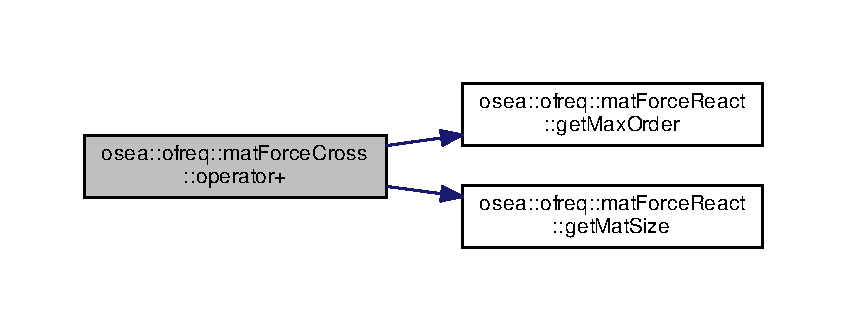
\includegraphics[width=350pt]{classosea_1_1ofreq_1_1mat_force_cross_a9cb8a17edf38bebb728ff47261175614_cgraph}
\end{center}
\end{figure}


\hypertarget{classosea_1_1ofreq_1_1mat_force_cross_af22b49c1536dc753f99b34a3eba1c8e7}{\index{osea\-::ofreq\-::mat\-Force\-Cross@{osea\-::ofreq\-::mat\-Force\-Cross}!operator-\/@{operator-\/}}
\index{operator-\/@{operator-\/}!osea::ofreq::matForceCross@{osea\-::ofreq\-::mat\-Force\-Cross}}
\subsubsection[{operator-\/}]{\setlength{\rightskip}{0pt plus 5cm}{\bf mat\-Force\-Cross} mat\-Force\-Cross\-::operator-\/ (
\begin{DoxyParamCaption}
\item[{{\bf mat\-Force\-Cross} \&}]{force\-Other}
\end{DoxyParamCaption}
)}}\label{classosea_1_1ofreq_1_1mat_force_cross_af22b49c1536dc753f99b34a3eba1c8e7}


Operator overload to subtract two \hyperlink{classosea_1_1ofreq_1_1mat_force_cross}{mat\-Force\-Cross} objects together. 

This overloads the -\/ operator to subtract two \hyperlink{classosea_1_1ofreq_1_1mat_force_cross}{mat\-Force\-Cross} objects together. Functions are subtracted on a per-\/derivative basis. The function recognizes the derivative matrices contained within each object. Only derivatives of the same order are subtracted together. Order of operations does matter. The function also checks the linked body parameter. Only objects with the same linked body are added together. 
\begin{DoxyParams}{Parameters}
{\em force\-Other} & The other objects of type \hyperlink{classosea_1_1ofreq_1_1mat_force_cross}{mat\-Force\-Cross} that will be subtracted. force\-Other is always subtracted from the calling object. \\
\hline
\end{DoxyParams}
\begin{DoxyReturn}{Returns}
Returns an object of type \hyperlink{classosea_1_1ofreq_1_1mat_force_cross}{mat\-Force\-Cross}. The new object will contain the same order of derivatives as the highest derivative of the two subtracted functions. 
\end{DoxyReturn}


Definition at line 145 of file matforcecross.\-cpp.



Here is the call graph for this function\-:
\nopagebreak
\begin{figure}[H]
\begin{center}
\leavevmode
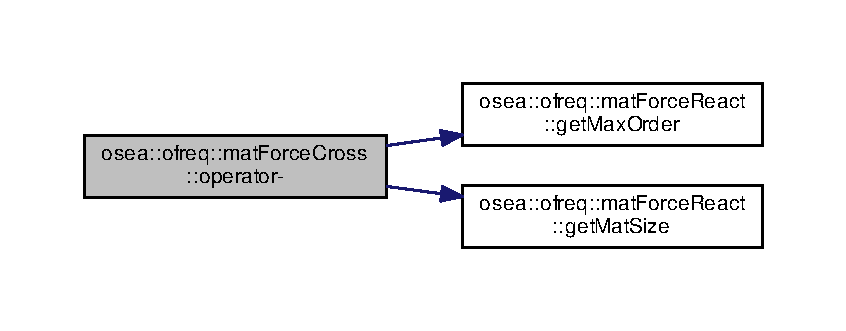
\includegraphics[width=350pt]{classosea_1_1ofreq_1_1mat_force_cross_af22b49c1536dc753f99b34a3eba1c8e7_cgraph}
\end{center}
\end{figure}


\hypertarget{classosea_1_1ofreq_1_1mat_force_cross_a546ca085994682e1e8160ce3014ffaae}{\index{osea\-::ofreq\-::mat\-Force\-Cross@{osea\-::ofreq\-::mat\-Force\-Cross}!set\-Linked\-Body@{set\-Linked\-Body}}
\index{set\-Linked\-Body@{set\-Linked\-Body}!osea::ofreq::matForceCross@{osea\-::ofreq\-::mat\-Force\-Cross}}
\subsubsection[{set\-Linked\-Body}]{\setlength{\rightskip}{0pt plus 5cm}void mat\-Force\-Cross\-::set\-Linked\-Body (
\begin{DoxyParamCaption}
\item[{{\bf mat\-Body} \&}]{Bod\-In}
\end{DoxyParamCaption}
)}}\label{classosea_1_1ofreq_1_1mat_force_cross_a546ca085994682e1e8160ce3014ffaae}
Set linked body for cross body object. 
\begin{DoxyParams}{Parameters}
{\em Bod\-In} & pointer to the \hyperlink{classosea_1_1ofreq_1_1mat_body}{mat\-Body} object that this linked force relates to. \\
\hline
\end{DoxyParams}


Definition at line 230 of file matforcecross.\-cpp.



Here is the call graph for this function\-:
\nopagebreak
\begin{figure}[H]
\begin{center}
\leavevmode
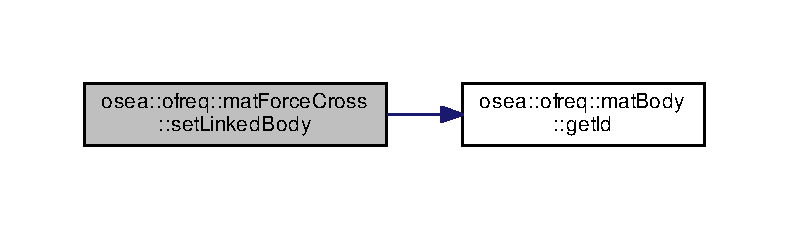
\includegraphics[width=350pt]{classosea_1_1ofreq_1_1mat_force_cross_a546ca085994682e1e8160ce3014ffaae_cgraph}
\end{center}
\end{figure}


\hypertarget{classosea_1_1ofreq_1_1mat_force_cross_a285c83c27df6413f90665480d2f3a4ed}{\index{osea\-::ofreq\-::mat\-Force\-Cross@{osea\-::ofreq\-::mat\-Force\-Cross}!set\-Linked\-Id@{set\-Linked\-Id}}
\index{set\-Linked\-Id@{set\-Linked\-Id}!osea::ofreq::matForceCross@{osea\-::ofreq\-::mat\-Force\-Cross}}
\subsubsection[{set\-Linked\-Id}]{\setlength{\rightskip}{0pt plus 5cm}void mat\-Force\-Cross\-::set\-Linked\-Id (
\begin{DoxyParamCaption}
\item[{int}]{bod\-Id}
\end{DoxyParamCaption}
)}}\label{classosea_1_1ofreq_1_1mat_force_cross_a285c83c27df6413f90665480d2f3a4ed}


Sets the id of the linked body. 

Sets the id of the linked body. The id is like the body's name. This is normally the index of the body within the vector of other bodies. 
\begin{DoxyParams}{Parameters}
{\em bod\-Id} & The integer of the body id. This is normally the index of the body within the vector of other bodies. \\
\hline
\end{DoxyParams}


Definition at line 245 of file matforcecross.\-cpp.



The documentation for this class was generated from the following files\-:\begin{DoxyCompactItemize}
\item 
/home/\-Ship\-\_\-\-Design/\-Projects/\-D\-M\-S1305 Open\-S\-E\-A/master/200\-\_\-src/bin/ofreq/motion\-\_\-solver/\hyperlink{matforcecross_8h}{matforcecross.\-h}\item 
/home/\-Ship\-\_\-\-Design/\-Projects/\-D\-M\-S1305 Open\-S\-E\-A/master/200\-\_\-src/bin/ofreq/motion\-\_\-solver/\hyperlink{matforcecross_8cpp}{matforcecross.\-cpp}\end{DoxyCompactItemize}

\hypertarget{classosea_1_1ofreq_1_1mat_force_react}{\section{osea\-:\-:ofreq\-:\-:mat\-Force\-React Class Reference}
\label{classosea_1_1ofreq_1_1mat_force_react}\index{osea\-::ofreq\-::mat\-Force\-React@{osea\-::ofreq\-::mat\-Force\-React}}
}


{\ttfamily \#include $<$matforcereact.\-h$>$}



Inheritance diagram for osea\-:\-:ofreq\-:\-:mat\-Force\-React\-:
\nopagebreak
\begin{figure}[H]
\begin{center}
\leavevmode
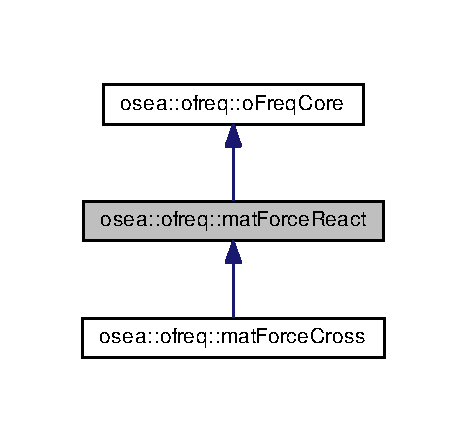
\includegraphics[width=224pt]{classosea_1_1ofreq_1_1mat_force_react__inherit__graph}
\end{center}
\end{figure}


Collaboration diagram for osea\-:\-:ofreq\-:\-:mat\-Force\-React\-:
\nopagebreak
\begin{figure}[H]
\begin{center}
\leavevmode
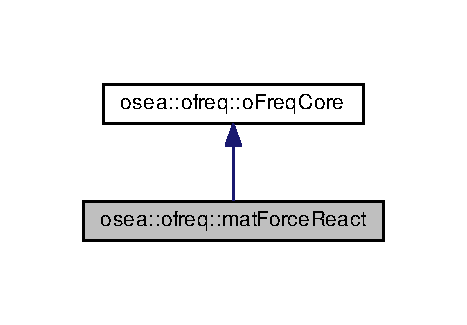
\includegraphics[width=224pt]{classosea_1_1ofreq_1_1mat_force_react__coll__graph}
\end{center}
\end{figure}
\subsection*{Public Member Functions}
\begin{DoxyCompactItemize}
\item 
\hyperlink{classosea_1_1ofreq_1_1mat_force_react_a7ab246a401282eb86db5db5036eedc48}{mat\-Force\-React} ()
\item 
\hyperlink{classosea_1_1ofreq_1_1mat_force_react_a2587d123951b9f092bef18b694a59673}{mat\-Force\-React} (std\-::vector$<$ arma\-::cx\-\_\-mat $>$ force\-In)
\begin{DoxyCompactList}\small\item\em The constructor. Takes a vector of complex matrices and stores them as derivatives. \end{DoxyCompactList}\item 
virtual \hyperlink{classosea_1_1ofreq_1_1mat_force_react_a4c70511a7f49650d56b0a2ed42bf4f8b}{$\sim$mat\-Force\-React} ()
\item 
virtual \hyperlink{classosea_1_1ofreq_1_1mat_force_react}{mat\-Force\-React} \hyperlink{classosea_1_1ofreq_1_1mat_force_react_a8f65b2f67fd6169167cc9735370c99eb}{operator+} (\hyperlink{classosea_1_1ofreq_1_1mat_force_react}{mat\-Force\-React} \&force\-Other)
\begin{DoxyCompactList}\small\item\em Operator overload to add two \hyperlink{classosea_1_1ofreq_1_1mat_force_react}{mat\-Force\-React} objects together. \end{DoxyCompactList}\item 
virtual \hyperlink{classosea_1_1ofreq_1_1mat_force_react}{mat\-Force\-React} \hyperlink{classosea_1_1ofreq_1_1mat_force_react_ad3be4d341c5fdabf28634cf102a8fbc9}{operator-\/} (\hyperlink{classosea_1_1ofreq_1_1mat_force_react}{mat\-Force\-React} \&force\-Other)
\begin{DoxyCompactList}\small\item\em Operator overload to subtract two \hyperlink{classosea_1_1ofreq_1_1mat_force_react}{mat\-Force\-React} objects together. \end{DoxyCompactList}\item 
int \hyperlink{classosea_1_1ofreq_1_1mat_force_react_aa163ad7393a29dc15fc2c490f88ef5cd}{get\-Max\-Order} ()
\begin{DoxyCompactList}\small\item\em The maximum order of the derivatives. \end{DoxyCompactList}\item 
arma\-::cx\-\_\-mat \hyperlink{classosea_1_1ofreq_1_1mat_force_react_a916eb8547f09eb3bf67092f0f64ac59c}{get\-Derivative} (int order)
\begin{DoxyCompactList}\small\item\em \hyperlink{classosea_1_1ofreq_1_1_derivative}{Derivative} Returns the complex matrix for only the order of derivative specified. \end{DoxyCompactList}\item 
void \hyperlink{classosea_1_1ofreq_1_1mat_force_react_ad887dadbcd1dcd2fdf9c78ac39fcacd4}{set\-Derivative} (int order, arma\-::cx\-\_\-mat Coeff)
\begin{DoxyCompactList}\small\item\em Inputs a derivative matrix. \end{DoxyCompactList}\item 
std\-::vector$<$ arma\-::cx\-\_\-mat $>$ \& \hyperlink{classosea_1_1ofreq_1_1mat_force_react_a52f785374b8e9b6e4d33e0eac95c8622}{list\-Derivative} ()
\begin{DoxyCompactList}\small\item\em Provides direct access to the vector of derivatives. \end{DoxyCompactList}\item 
arma\-::cx\-\_\-mat \& \hyperlink{classosea_1_1ofreq_1_1mat_force_react_af05d5675a035a111264a37472e9ba479}{list\-Derivative} (unsigned int index)
\begin{DoxyCompactList}\small\item\em Provides direct access to the derivative specified by the index. \end{DoxyCompactList}\item 
void \hyperlink{classosea_1_1ofreq_1_1mat_force_react_a778765a5296698179dee923397032756}{set\-Id} (int num)
\begin{DoxyCompactList}\small\item\em Sets the force id number for the object. \end{DoxyCompactList}\item 
int \hyperlink{classosea_1_1ofreq_1_1mat_force_react_ad6416ceeafeb1f1852911fce0536b7f0}{get\-Id} ()
\begin{DoxyCompactList}\small\item\em Returns the force id number for the object. \end{DoxyCompactList}\item 
int \hyperlink{classosea_1_1ofreq_1_1mat_force_react_a9e9d9119e2ca2b49d0faea0897f7e300}{get\-Mat\-Size} ()
\begin{DoxyCompactList}\small\item\em Returns the size of the matrix in each order of derivative. \end{DoxyCompactList}\end{DoxyCompactItemize}
\subsection*{Protected Attributes}
\begin{DoxyCompactItemize}
\item 
std\-::vector$<$ arma\-::cx\-\_\-mat $>$ \hyperlink{classosea_1_1ofreq_1_1mat_force_react_a827cccb59204d98738a4d98b78942b45}{pderiv}
\begin{DoxyCompactList}\small\item\em Defines the vector of derivatives. \end{DoxyCompactList}\item 
int \hyperlink{classosea_1_1ofreq_1_1mat_force_react_a890a6fbcf9900d4a37ff05533f350f50}{p\-Id}
\begin{DoxyCompactList}\small\item\em the number of the object in the outside vector that contains it. \end{DoxyCompactList}\end{DoxyCompactItemize}
\subsection*{Additional Inherited Members}


\subsection{Detailed Description}
This class holds data for reactive force matrix whch includes force coefficients. 

\subsection{Constructor \& Destructor Documentation}
\hypertarget{classosea_1_1ofreq_1_1mat_force_react_a7ab246a401282eb86db5db5036eedc48}{\index{osea\-::ofreq\-::mat\-Force\-React@{osea\-::ofreq\-::mat\-Force\-React}!mat\-Force\-React@{mat\-Force\-React}}
\index{mat\-Force\-React@{mat\-Force\-React}!osea::ofreq::matForceReact@{osea\-::ofreq\-::mat\-Force\-React}}
\subsubsection[{mat\-Force\-React}]{\setlength{\rightskip}{0pt plus 5cm}mat\-Force\-React\-::mat\-Force\-React (
\begin{DoxyParamCaption}
{}
\end{DoxyParamCaption}
)}}\label{classosea_1_1ofreq_1_1mat_force_react_a7ab246a401282eb86db5db5036eedc48}
The default constructor. \hypertarget{classosea_1_1ofreq_1_1mat_force_react_a2587d123951b9f092bef18b694a59673}{\index{osea\-::ofreq\-::mat\-Force\-React@{osea\-::ofreq\-::mat\-Force\-React}!mat\-Force\-React@{mat\-Force\-React}}
\index{mat\-Force\-React@{mat\-Force\-React}!osea::ofreq::matForceReact@{osea\-::ofreq\-::mat\-Force\-React}}
\subsubsection[{mat\-Force\-React}]{\setlength{\rightskip}{0pt plus 5cm}osea\-::ofreq\-::mat\-Force\-React\-::mat\-Force\-React (
\begin{DoxyParamCaption}
\item[{std\-::vector$<$ arma\-::cx\-\_\-mat $>$}]{force\-In}
\end{DoxyParamCaption}
)}}\label{classosea_1_1ofreq_1_1mat_force_react_a2587d123951b9f092bef18b694a59673}


The constructor. Takes a vector of complex matrices and stores them as derivatives. 

The constructor. Takes a vector of complex matrices and stores them as derivatives. Assumes that the matrices in the vector are order in sequence of increasing order of derivative. (index 0 = derivative order 0.) 
\begin{DoxyParams}{Parameters}
{\em force\-In} & The list of forces. \\
\hline
\end{DoxyParams}
\hypertarget{classosea_1_1ofreq_1_1mat_force_react_a4c70511a7f49650d56b0a2ed42bf4f8b}{\index{osea\-::ofreq\-::mat\-Force\-React@{osea\-::ofreq\-::mat\-Force\-React}!$\sim$mat\-Force\-React@{$\sim$mat\-Force\-React}}
\index{$\sim$mat\-Force\-React@{$\sim$mat\-Force\-React}!osea::ofreq::matForceReact@{osea\-::ofreq\-::mat\-Force\-React}}
\subsubsection[{$\sim$mat\-Force\-React}]{\setlength{\rightskip}{0pt plus 5cm}mat\-Force\-React\-::$\sim$mat\-Force\-React (
\begin{DoxyParamCaption}
{}
\end{DoxyParamCaption}
)\hspace{0.3cm}{\ttfamily [virtual]}}}\label{classosea_1_1ofreq_1_1mat_force_react_a4c70511a7f49650d56b0a2ed42bf4f8b}
The default destructor, nothing happens here. 

\subsection{Member Function Documentation}
\hypertarget{classosea_1_1ofreq_1_1mat_force_react_a916eb8547f09eb3bf67092f0f64ac59c}{\index{osea\-::ofreq\-::mat\-Force\-React@{osea\-::ofreq\-::mat\-Force\-React}!get\-Derivative@{get\-Derivative}}
\index{get\-Derivative@{get\-Derivative}!osea::ofreq::matForceReact@{osea\-::ofreq\-::mat\-Force\-React}}
\subsubsection[{get\-Derivative}]{\setlength{\rightskip}{0pt plus 5cm}cx\-\_\-mat mat\-Force\-React\-::get\-Derivative (
\begin{DoxyParamCaption}
\item[{int}]{order}
\end{DoxyParamCaption}
)}}\label{classosea_1_1ofreq_1_1mat_force_react_a916eb8547f09eb3bf67092f0f64ac59c}


\hyperlink{classosea_1_1ofreq_1_1_derivative}{Derivative} Returns the complex matrix for only the order of derivative specified. 

\hyperlink{classosea_1_1ofreq_1_1_derivative}{Derivative} Returns the complex matrix for only the order of derivative specified. 
\begin{DoxyParams}{Parameters}
{\em order} & Integer input to specify the order of the derivative. \\
\hline
\end{DoxyParams}
\begin{DoxyReturn}{Returns}
Returns a complex matrix that contains the force coefficients for the given order of derivative. Passed as a value. 
\end{DoxyReturn}


Here is the caller graph for this function\-:
\nopagebreak
\begin{figure}[H]
\begin{center}
\leavevmode
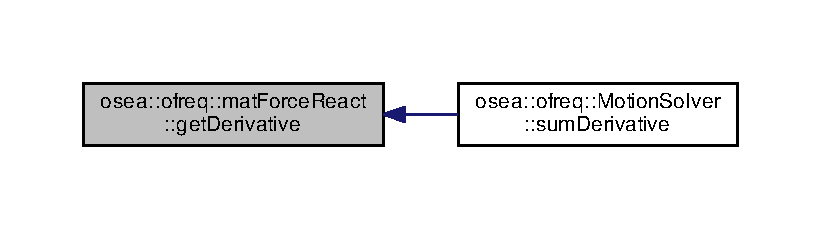
\includegraphics[width=350pt]{classosea_1_1ofreq_1_1mat_force_react_a916eb8547f09eb3bf67092f0f64ac59c_icgraph}
\end{center}
\end{figure}


\hypertarget{classosea_1_1ofreq_1_1mat_force_react_ad6416ceeafeb1f1852911fce0536b7f0}{\index{osea\-::ofreq\-::mat\-Force\-React@{osea\-::ofreq\-::mat\-Force\-React}!get\-Id@{get\-Id}}
\index{get\-Id@{get\-Id}!osea::ofreq::matForceReact@{osea\-::ofreq\-::mat\-Force\-React}}
\subsubsection[{get\-Id}]{\setlength{\rightskip}{0pt plus 5cm}int mat\-Force\-React\-::get\-Id (
\begin{DoxyParamCaption}
{}
\end{DoxyParamCaption}
)}}\label{classosea_1_1ofreq_1_1mat_force_react_ad6416ceeafeb1f1852911fce0536b7f0}


Returns the force id number for the object. 

This is similar to the name parameter in other force objects. It is an identifier. In this case, a numerical identifier. Normally correlates to the objects index in a vector of other objects of the same class. \begin{DoxyReturn}{Returns}
Returns the force id number, integer data type. 
\end{DoxyReturn}
\hypertarget{classosea_1_1ofreq_1_1mat_force_react_a9e9d9119e2ca2b49d0faea0897f7e300}{\index{osea\-::ofreq\-::mat\-Force\-React@{osea\-::ofreq\-::mat\-Force\-React}!get\-Mat\-Size@{get\-Mat\-Size}}
\index{get\-Mat\-Size@{get\-Mat\-Size}!osea::ofreq::matForceReact@{osea\-::ofreq\-::mat\-Force\-React}}
\subsubsection[{get\-Mat\-Size}]{\setlength{\rightskip}{0pt plus 5cm}int mat\-Force\-React\-::get\-Mat\-Size (
\begin{DoxyParamCaption}
{}
\end{DoxyParamCaption}
)}}\label{classosea_1_1ofreq_1_1mat_force_react_a9e9d9119e2ca2b49d0faea0897f7e300}


Returns the size of the matrix in each order of derivative. 

Returns the size of the matrix in each order of derivative. Integer output type. \begin{DoxyReturn}{Returns}
Returns the size of the matrix in each order of derivative. 
\end{DoxyReturn}


Here is the caller graph for this function\-:
\nopagebreak
\begin{figure}[H]
\begin{center}
\leavevmode
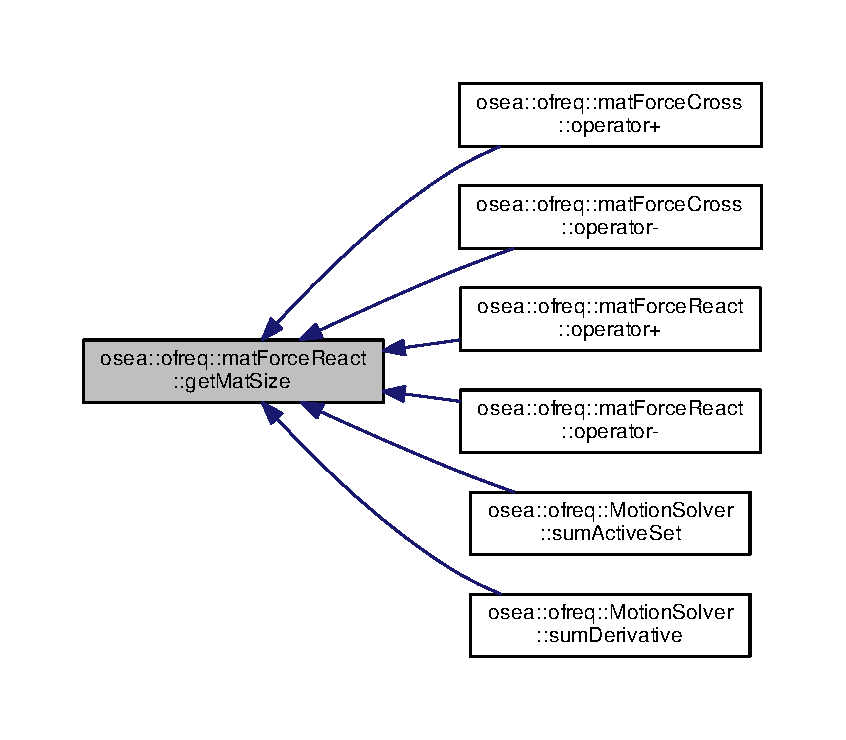
\includegraphics[width=350pt]{classosea_1_1ofreq_1_1mat_force_react_a9e9d9119e2ca2b49d0faea0897f7e300_icgraph}
\end{center}
\end{figure}


\hypertarget{classosea_1_1ofreq_1_1mat_force_react_aa163ad7393a29dc15fc2c490f88ef5cd}{\index{osea\-::ofreq\-::mat\-Force\-React@{osea\-::ofreq\-::mat\-Force\-React}!get\-Max\-Order@{get\-Max\-Order}}
\index{get\-Max\-Order@{get\-Max\-Order}!osea::ofreq::matForceReact@{osea\-::ofreq\-::mat\-Force\-React}}
\subsubsection[{get\-Max\-Order}]{\setlength{\rightskip}{0pt plus 5cm}int mat\-Force\-React\-::get\-Max\-Order (
\begin{DoxyParamCaption}
{}
\end{DoxyParamCaption}
)}}\label{classosea_1_1ofreq_1_1mat_force_react_aa163ad7393a29dc15fc2c490f88ef5cd}


The maximum order of the derivatives. 

The maximum order of the derivatives (Integer). Also the total size of the vector containing the derivatives. \begin{DoxyReturn}{Returns}
Returns the maximum order of derivatives in the force. 
\end{DoxyReturn}


Here is the caller graph for this function\-:
\nopagebreak
\begin{figure}[H]
\begin{center}
\leavevmode
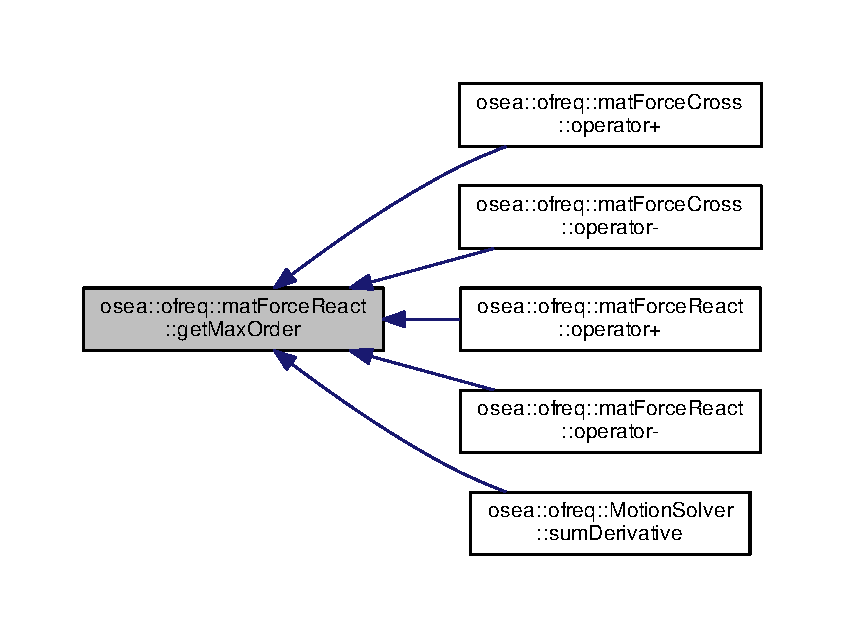
\includegraphics[width=350pt]{classosea_1_1ofreq_1_1mat_force_react_aa163ad7393a29dc15fc2c490f88ef5cd_icgraph}
\end{center}
\end{figure}


\hypertarget{classosea_1_1ofreq_1_1mat_force_react_a52f785374b8e9b6e4d33e0eac95c8622}{\index{osea\-::ofreq\-::mat\-Force\-React@{osea\-::ofreq\-::mat\-Force\-React}!list\-Derivative@{list\-Derivative}}
\index{list\-Derivative@{list\-Derivative}!osea::ofreq::matForceReact@{osea\-::ofreq\-::mat\-Force\-React}}
\subsubsection[{list\-Derivative}]{\setlength{\rightskip}{0pt plus 5cm}vector$<$ cx\-\_\-mat $>$ \& mat\-Force\-React\-::list\-Derivative (
\begin{DoxyParamCaption}
{}
\end{DoxyParamCaption}
)}}\label{classosea_1_1ofreq_1_1mat_force_react_a52f785374b8e9b6e4d33e0eac95c8622}


Provides direct access to the vector of derivatives. 

Provides direct access to the vector of derivatives. Allows for use of vector operations on the derivatives object. \begin{DoxyReturn}{Returns}
Returns reference to the vector of complex matrices which contain the derivatives. Variable passed by reference. 
\end{DoxyReturn}
\hypertarget{classosea_1_1ofreq_1_1mat_force_react_af05d5675a035a111264a37472e9ba479}{\index{osea\-::ofreq\-::mat\-Force\-React@{osea\-::ofreq\-::mat\-Force\-React}!list\-Derivative@{list\-Derivative}}
\index{list\-Derivative@{list\-Derivative}!osea::ofreq::matForceReact@{osea\-::ofreq\-::mat\-Force\-React}}
\subsubsection[{list\-Derivative}]{\setlength{\rightskip}{0pt plus 5cm}cx\-\_\-mat \& mat\-Force\-React\-::list\-Derivative (
\begin{DoxyParamCaption}
\item[{unsigned int}]{index}
\end{DoxyParamCaption}
)}}\label{classosea_1_1ofreq_1_1mat_force_react_af05d5675a035a111264a37472e9ba479}


Provides direct access to the derivative specified by the index. 

Allows for direct access to edit the derivative or just retrieve information from. Index is also the order of the derivative. 
\begin{DoxyParams}{Parameters}
{\em index} & Unsigned integer. Specifies the index of which derivative to retrieve from the list. \\
\hline
\end{DoxyParams}
\begin{DoxyReturn}{Returns}
Complex matrix returned. Returns the complex matrix for the derivative specified by the index. Returned variable is passed by reference. 
\end{DoxyReturn}
\hypertarget{classosea_1_1ofreq_1_1mat_force_react_a8f65b2f67fd6169167cc9735370c99eb}{\index{osea\-::ofreq\-::mat\-Force\-React@{osea\-::ofreq\-::mat\-Force\-React}!operator+@{operator+}}
\index{operator+@{operator+}!osea::ofreq::matForceReact@{osea\-::ofreq\-::mat\-Force\-React}}
\subsubsection[{operator+}]{\setlength{\rightskip}{0pt plus 5cm}{\bf mat\-Force\-React} mat\-Force\-React\-::operator+ (
\begin{DoxyParamCaption}
\item[{{\bf mat\-Force\-React} \&}]{force\-Other}
\end{DoxyParamCaption}
)\hspace{0.3cm}{\ttfamily [virtual]}}}\label{classosea_1_1ofreq_1_1mat_force_react_a8f65b2f67fd6169167cc9735370c99eb}


Operator overload to add two \hyperlink{classosea_1_1ofreq_1_1mat_force_react}{mat\-Force\-React} objects together. 

This overloads the + operator to add two \hyperlink{classosea_1_1ofreq_1_1mat_force_react}{mat\-Force\-React} objects together. Functions are added on a per-\/derivative basis. The function recognizes the derivative matrices contained within each object. Only derivatives of the same order are added together. 
\begin{DoxyParams}{Parameters}
{\em force\-Other} & The other objects of type \hyperlink{classosea_1_1ofreq_1_1mat_force_react}{mat\-Force\-React} that will be added. \\
\hline
\end{DoxyParams}
\begin{DoxyReturn}{Returns}
Returns an object of type \hyperlink{classosea_1_1ofreq_1_1mat_force_react}{mat\-Force\-React}. The new object will contain the same order of derivatives as the highest derivative of the two added functions. 
\end{DoxyReturn}


Here is the call graph for this function\-:
\nopagebreak
\begin{figure}[H]
\begin{center}
\leavevmode
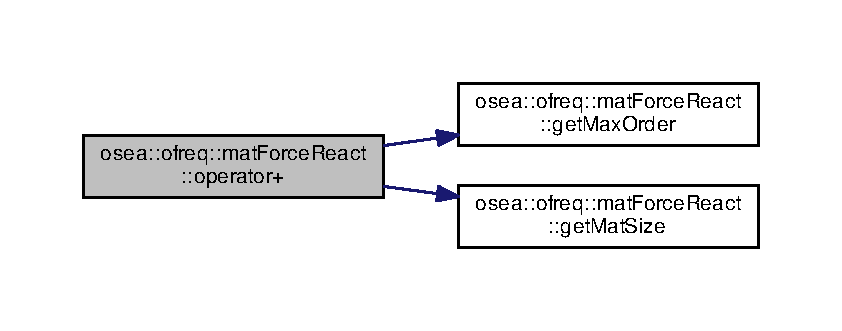
\includegraphics[width=350pt]{classosea_1_1ofreq_1_1mat_force_react_a8f65b2f67fd6169167cc9735370c99eb_cgraph}
\end{center}
\end{figure}


\hypertarget{classosea_1_1ofreq_1_1mat_force_react_ad3be4d341c5fdabf28634cf102a8fbc9}{\index{osea\-::ofreq\-::mat\-Force\-React@{osea\-::ofreq\-::mat\-Force\-React}!operator-\/@{operator-\/}}
\index{operator-\/@{operator-\/}!osea::ofreq::matForceReact@{osea\-::ofreq\-::mat\-Force\-React}}
\subsubsection[{operator-\/}]{\setlength{\rightskip}{0pt plus 5cm}{\bf mat\-Force\-React} mat\-Force\-React\-::operator-\/ (
\begin{DoxyParamCaption}
\item[{{\bf mat\-Force\-React} \&}]{force\-Other}
\end{DoxyParamCaption}
)\hspace{0.3cm}{\ttfamily [virtual]}}}\label{classosea_1_1ofreq_1_1mat_force_react_ad3be4d341c5fdabf28634cf102a8fbc9}


Operator overload to subtract two \hyperlink{classosea_1_1ofreq_1_1mat_force_react}{mat\-Force\-React} objects together. 

This overloads the -\/ operator to subtract two \hyperlink{classosea_1_1ofreq_1_1mat_force_react}{mat\-Force\-React} objects together. Functions are subtracted on a per-\/derivative basis. The function recognizes the derivative matrices contained within each object. Only derivatives of the same order are subtracted together. Order of operations does matter. 
\begin{DoxyParams}{Parameters}
{\em force\-Other} & The other objects of type \hyperlink{classosea_1_1ofreq_1_1mat_force_react}{mat\-Force\-React} that will be subtracted. force\-Other is always subtracted from the calling object. \\
\hline
\end{DoxyParams}
\begin{DoxyReturn}{Returns}
Returns an object of type \hyperlink{classosea_1_1ofreq_1_1mat_force_react}{mat\-Force\-React}. The new object will contain the same order of derivatives as the highest derivative of the two subtracted functions. 
\end{DoxyReturn}


Here is the call graph for this function\-:
\nopagebreak
\begin{figure}[H]
\begin{center}
\leavevmode
\includegraphics[width=350pt]{classosea_1_1ofreq_1_1mat_force_react_ad3be4d341c5fdabf28634cf102a8fbc9_cgraph}
\end{center}
\end{figure}


\hypertarget{classosea_1_1ofreq_1_1mat_force_react_ad887dadbcd1dcd2fdf9c78ac39fcacd4}{\index{osea\-::ofreq\-::mat\-Force\-React@{osea\-::ofreq\-::mat\-Force\-React}!set\-Derivative@{set\-Derivative}}
\index{set\-Derivative@{set\-Derivative}!osea::ofreq::matForceReact@{osea\-::ofreq\-::mat\-Force\-React}}
\subsubsection[{set\-Derivative}]{\setlength{\rightskip}{0pt plus 5cm}void mat\-Force\-React\-::set\-Derivative (
\begin{DoxyParamCaption}
\item[{int}]{order, }
\item[{arma\-::cx\-\_\-mat}]{Coeff}
\end{DoxyParamCaption}
)}}\label{classosea_1_1ofreq_1_1mat_force_react_ad887dadbcd1dcd2fdf9c78ac39fcacd4}


Inputs a derivative matrix. 


\begin{DoxyParams}{Parameters}
{\em order} & The order of the derivative matrix. Also is sequence in the vector that contains the matrices. \\
\hline
{\em Coeff} & The matrix of complex numbers that contains the force coefficients for the derivative. Passed as a value, not a reference. \\
\hline
\end{DoxyParams}
\hypertarget{classosea_1_1ofreq_1_1mat_force_react_a778765a5296698179dee923397032756}{\index{osea\-::ofreq\-::mat\-Force\-React@{osea\-::ofreq\-::mat\-Force\-React}!set\-Id@{set\-Id}}
\index{set\-Id@{set\-Id}!osea::ofreq::matForceReact@{osea\-::ofreq\-::mat\-Force\-React}}
\subsubsection[{set\-Id}]{\setlength{\rightskip}{0pt plus 5cm}void mat\-Force\-React\-::set\-Id (
\begin{DoxyParamCaption}
\item[{int}]{num}
\end{DoxyParamCaption}
)}}\label{classosea_1_1ofreq_1_1mat_force_react_a778765a5296698179dee923397032756}


Sets the force id number for the object. 

This is similar to the name parameter in other force objects. It is an identifier. In this case, a numerical identifier. Normally correlates to the objects index in a vector of other objects of the same class. 
\begin{DoxyParams}{Parameters}
{\em num} & The integer number to input as the objects integer id. \\
\hline
\end{DoxyParams}


\subsection{Member Data Documentation}
\hypertarget{classosea_1_1ofreq_1_1mat_force_react_a827cccb59204d98738a4d98b78942b45}{\index{osea\-::ofreq\-::mat\-Force\-React@{osea\-::ofreq\-::mat\-Force\-React}!pderiv@{pderiv}}
\index{pderiv@{pderiv}!osea::ofreq::matForceReact@{osea\-::ofreq\-::mat\-Force\-React}}
\subsubsection[{pderiv}]{\setlength{\rightskip}{0pt plus 5cm}std\-::vector$<$arma\-::cx\-\_\-mat$>$ osea\-::ofreq\-::mat\-Force\-React\-::pderiv\hspace{0.3cm}{\ttfamily [protected]}}}\label{classosea_1_1ofreq_1_1mat_force_react_a827cccb59204d98738a4d98b78942b45}


Defines the vector of derivatives. 

Defines the vector of derivatives. Each entry in vector represents the order of the derivative. \hypertarget{classosea_1_1ofreq_1_1mat_force_react_a890a6fbcf9900d4a37ff05533f350f50}{\index{osea\-::ofreq\-::mat\-Force\-React@{osea\-::ofreq\-::mat\-Force\-React}!p\-Id@{p\-Id}}
\index{p\-Id@{p\-Id}!osea::ofreq::matForceReact@{osea\-::ofreq\-::mat\-Force\-React}}
\subsubsection[{p\-Id}]{\setlength{\rightskip}{0pt plus 5cm}int osea\-::ofreq\-::mat\-Force\-React\-::p\-Id\hspace{0.3cm}{\ttfamily [protected]}}}\label{classosea_1_1ofreq_1_1mat_force_react_a890a6fbcf9900d4a37ff05533f350f50}


the number of the object in the outside vector that contains it. 

This is similar to the name parameter in other force objects. It is an identifier. In this case, a numerical identifier. Normally correlates to the objects index in a vector of other objects of the same class. 

The documentation for this class was generated from the following files\-:\begin{DoxyCompactItemize}
\item 
matforcereact.\-h\item 
matforcereact.\-cpp\end{DoxyCompactItemize}

\hypertarget{classosea_1_1ofreq_1_1_motion_model}{\section{osea\-:\-:ofreq\-:\-:Motion\-Model Class Reference}
\label{classosea_1_1ofreq_1_1_motion_model}\index{osea\-::ofreq\-::\-Motion\-Model@{osea\-::ofreq\-::\-Motion\-Model}}
}


{\ttfamily \#include $<$motionmodel.\-h$>$}



Inheritance diagram for osea\-:\-:ofreq\-:\-:Motion\-Model\-:
\nopagebreak
\begin{figure}[H]
\begin{center}
\leavevmode
\includegraphics[width=214pt]{classosea_1_1ofreq_1_1_motion_model__inherit__graph}
\end{center}
\end{figure}


Collaboration diagram for osea\-:\-:ofreq\-:\-:Motion\-Model\-:
\nopagebreak
\begin{figure}[H]
\begin{center}
\leavevmode
\includegraphics[width=214pt]{classosea_1_1ofreq_1_1_motion_model__coll__graph}
\end{center}
\end{figure}
\subsection*{Public Member Functions}
\begin{DoxyCompactItemize}
\item 
\hyperlink{classosea_1_1ofreq_1_1_motion_model_a5a5e4bba0f6ca24e1fdd316458f4f824}{Motion\-Model} ()
\item 
\hyperlink{classosea_1_1ofreq_1_1_motion_model_aace42c5711b5486181e986add9a72b8f}{Motion\-Model} (std\-::vector$<$ \hyperlink{classosea_1_1ofreq_1_1_body}{Body} $>$ \&list\-Bod\-In)
\begin{DoxyCompactList}\small\item\em Constructor. This is the preferred constructor as it supplies the body data. \end{DoxyCompactList}\item 
virtual \hyperlink{classosea_1_1ofreq_1_1_motion_model_ac48a359c77d9efe39d4ec8c9e862a1cd}{$\sim$\-Motion\-Model} ()
\item 
void \hyperlink{classosea_1_1ofreq_1_1_motion_model_a92f6b9639a82aef868dbaf8445276d3c}{setlist\-Body} (std\-::vector$<$ \hyperlink{classosea_1_1ofreq_1_1_body}{Body} $>$ \&list\-Bod\-In)
\begin{DoxyCompactList}\small\item\em Inputs the list of body data. \end{DoxyCompactList}\item 
void \hyperlink{classosea_1_1ofreq_1_1_motion_model_a713b903a3e78141fff2af9c045755ffb}{set\-Body} (int bod)
\begin{DoxyCompactList}\small\item\em Sets the index for the body that all calculations are based on. \end{DoxyCompactList}\item 
int \hyperlink{classosea_1_1ofreq_1_1_motion_model_a72ee8cafa92a2dee644124d051856207}{get\-Body} ()
\begin{DoxyCompactList}\small\item\em Gets the index for the body that all calculations are based on. \end{DoxyCompactList}\item 
bool \& \hyperlink{classosea_1_1ofreq_1_1_motion_model_af4d34bfa133e77f1527cee1aa36b02f4}{Coefficient\-Only} ()
\begin{DoxyCompactList}\small\item\em Determines whether the class should calculate force coefficients or actual force values. True = Calculate force coefficients only. False = Calculate force values. Default = (False) Calculate force values. \end{DoxyCompactList}\item 
bool \hyperlink{classosea_1_1ofreq_1_1_motion_model_afc54a14912e56315505ef5dbec28bd39}{get\-Active\-Only} ()
\begin{DoxyCompactList}\small\item\em Boolean to track whether only the active forces are requested. \end{DoxyCompactList}\item 
std\-::vector$<$ int $>$ \& \hyperlink{classosea_1_1ofreq_1_1_motion_model_ac4169ab37ab7d69f5030a0d67cb3dc86}{list\-Comp\-Cross\-Bod\-\_\-hydro} ()
\begin{DoxyCompactList}\small\item\em Records the index of the body object referenced by the cross body. \end{DoxyCompactList}\item 
int \& \hyperlink{classosea_1_1ofreq_1_1_motion_model_abe445279c6f964b5a64e046945249ea9}{list\-Comp\-Cross\-Bod\-\_\-hydro} (int crossbod\-In)
\begin{DoxyCompactList}\small\item\em Records the index of the body object referenced by the cross body. \end{DoxyCompactList}\item 
std\-::vector$<$ int $>$ \& \hyperlink{classosea_1_1ofreq_1_1_motion_model_a873a325f0017d73989cee1cdf8285b3c}{list\-Comp\-Cross\-Bod\-\_\-user} ()
\begin{DoxyCompactList}\small\item\em Records the index of the body object referenced by the cross body. \end{DoxyCompactList}\item 
int \& \hyperlink{classosea_1_1ofreq_1_1_motion_model_a63d9e54f8cbb434f67753fe737a89ee6}{list\-Comp\-Cross\-Bod\-\_\-user} (int crossbod\-In)
\begin{DoxyCompactList}\small\item\em Records the index of the body object referenced by the cross body. \end{DoxyCompactList}\item 
\hypertarget{classosea_1_1ofreq_1_1_motion_model_a27842d2b76ab078534c0626601da446b}{void \hyperlink{classosea_1_1ofreq_1_1_motion_model_a27842d2b76ab078534c0626601da446b}{Reset} ()}\label{classosea_1_1ofreq_1_1_motion_model_a27842d2b76ab078534c0626601da446b}

\begin{DoxyCompactList}\small\item\em Resets the class data to have all input coefficients. Any evaluation after a reset will produce a value of zero. \hyperlink{classosea_1_1ofreq_1_1_force}{Force} coefficients will be zero and force values will be zero. \end{DoxyCompactList}\item 
void \hyperlink{classosea_1_1ofreq_1_1_motion_model_a18e880b4a0b1a1d1c385bc3be3524440}{set\-Freq} (double freq)
\begin{DoxyCompactList}\small\item\em Sets the current operating frequency for the function. Only necessary when calculating true forces and using derivatives defined in the motion model. Otherwise, you can safely ignore this function. \end{DoxyCompactList}\item 
double \hyperlink{classosea_1_1ofreq_1_1_motion_model_a3461ede3739b468b6bab3a05f94093cc}{get\-Freq} ()
\begin{DoxyCompactList}\small\item\em Gets the current operating frequency for the function. Only necessary when calculating true forces and using derivatives defined in the motion model. Otherwise, you can safely ignore this function. \end{DoxyCompactList}\item 
void \hyperlink{classosea_1_1ofreq_1_1_motion_model_aaf761fac4693612a10771e38993431a0}{use\-Force\-Active\-\_\-user} (unsigned int force, unsigned int eqn)
\begin{DoxyCompactList}\small\item\em Passes information to the object to use input coefficients from the entry specified. \end{DoxyCompactList}\item 
void \hyperlink{classosea_1_1ofreq_1_1_motion_model_a6b402b9e9cfab05159732f38035434b5}{use\-Force\-Active\-\_\-user} (unsigned int force)
\begin{DoxyCompactList}\small\item\em Passes information to the object to use input coefficients from the entry specified. \end{DoxyCompactList}\item 
void \hyperlink{classosea_1_1ofreq_1_1_motion_model_a78243e9d9fd197b4675aad8b728de55e}{use\-Force\-Active\-\_\-user} ()
\begin{DoxyCompactList}\small\item\em Passes information to the object to use input coefficients from the entry specified. \end{DoxyCompactList}\item 
void \hyperlink{classosea_1_1ofreq_1_1_motion_model_a4d3e0590135e1a9f7ce954406f99ff44}{use\-Force\-Active\-\_\-hydro} (unsigned int force, unsigned int eqn)
\begin{DoxyCompactList}\small\item\em Passes information to the object to use input coefficients from the entry specified. \end{DoxyCompactList}\item 
void \hyperlink{classosea_1_1ofreq_1_1_motion_model_a59ac49cac82e8214a2e1420e2f02736b}{use\-Force\-Active\-\_\-hydro} (unsigned int force)
\begin{DoxyCompactList}\small\item\em Passes information to the object to use input coefficients from the entry specified. \end{DoxyCompactList}\item 
void \hyperlink{classosea_1_1ofreq_1_1_motion_model_afe1c219c16bd1b3eb63f49065872cec6}{use\-Force\-Active\-\_\-hydro} ()
\begin{DoxyCompactList}\small\item\em Passes information to the object to use input coefficients from the entry specified. \end{DoxyCompactList}\item 
void \hyperlink{classosea_1_1ofreq_1_1_motion_model_a7db1d1ebebe216d17efd7b38f2e9deec}{use\-Force\-React\-\_\-user} (unsigned int force, unsigned int ord, unsigned int eqn, unsigned int var)
\begin{DoxyCompactList}\small\item\em Passes information to the object to use input coefficients from the entry specified. \end{DoxyCompactList}\item 
void \hyperlink{classosea_1_1ofreq_1_1_motion_model_a26352f59cd049a551ff692c5feb0b387}{use\-Force\-React\-\_\-user} (unsigned int force, unsigned int ord, unsigned int eqn)
\begin{DoxyCompactList}\small\item\em Passes information to the object to use input coefficients from the entry specified. \end{DoxyCompactList}\item 
void \hyperlink{classosea_1_1ofreq_1_1_motion_model_afa99c39f1018471c2ce0793f5de6987b}{use\-Force\-React\-\_\-user} (unsigned int force, unsigned int ord)
\begin{DoxyCompactList}\small\item\em Passes information to the object to use input coefficients from the entry specified. \end{DoxyCompactList}\item 
void \hyperlink{classosea_1_1ofreq_1_1_motion_model_a805e8c1ff2fdb767543011b093ec8e86}{use\-Force\-React\-\_\-user} (unsigned int force)
\begin{DoxyCompactList}\small\item\em Passes information to the object to use input coefficients from the entry specified. \end{DoxyCompactList}\item 
void \hyperlink{classosea_1_1ofreq_1_1_motion_model_a6d362d62468bacc57f5be5efe27deb4a}{use\-Force\-React\-\_\-user} ()
\begin{DoxyCompactList}\small\item\em Passes information to the object to use input coefficients from the entry specified. \end{DoxyCompactList}\item 
void \hyperlink{classosea_1_1ofreq_1_1_motion_model_ae3d2c7527ea2daddc6a85b6e02febb45}{use\-Force\-React\-\_\-hydro} (unsigned int force, unsigned int ord, unsigned int eqn, unsigned int var)
\begin{DoxyCompactList}\small\item\em Passes information to the object to use input coefficients from the entry specified. \end{DoxyCompactList}\item 
void \hyperlink{classosea_1_1ofreq_1_1_motion_model_a95f023bebf06d16a31b7b493a46c3ba3}{use\-Force\-React\-\_\-hydro} (unsigned int force, unsigned int ord, unsigned int eqn)
\begin{DoxyCompactList}\small\item\em Passes information to the object to use input coefficients from the entry specified. \end{DoxyCompactList}\item 
void \hyperlink{classosea_1_1ofreq_1_1_motion_model_a51c60631ee1d3546bc1df88c04d50805}{use\-Force\-React\-\_\-hydro} (unsigned int force, unsigned int ord)
\begin{DoxyCompactList}\small\item\em Passes information to the object to use input coefficients from the entry specified. \end{DoxyCompactList}\item 
void \hyperlink{classosea_1_1ofreq_1_1_motion_model_a62b3143f0a56d3cb5d8ffcc7eaf1968e}{use\-Force\-React\-\_\-hydro} (unsigned int force)
\begin{DoxyCompactList}\small\item\em Passes information to the object to use input coefficients from the entry specified. \end{DoxyCompactList}\item 
void \hyperlink{classosea_1_1ofreq_1_1_motion_model_a081dd7c11656da25fafa08f994685e48}{use\-Force\-React\-\_\-hydro} ()
\begin{DoxyCompactList}\small\item\em Passes information to the object to use input coefficients from the entry specified. \end{DoxyCompactList}\item 
void \hyperlink{classosea_1_1ofreq_1_1_motion_model_a1159117995080d2b62e50fceaeb29778}{use\-Force\-Cross\-\_\-user} (unsigned int force, unsigned int ord, unsigned int eqn, unsigned int var)
\begin{DoxyCompactList}\small\item\em Passes information to the object to use input coefficients from the entry specified. \end{DoxyCompactList}\item 
void \hyperlink{classosea_1_1ofreq_1_1_motion_model_a3eabe29c2306d9a36445cfb4b27c4b02}{use\-Force\-Cross\-\_\-user} (unsigned int force, unsigned int ord, unsigned int eqn)
\begin{DoxyCompactList}\small\item\em Passes information to the object to use input coefficients from the entry specified. \end{DoxyCompactList}\item 
void \hyperlink{classosea_1_1ofreq_1_1_motion_model_ac507056503b23bddf1e5fcf5850b7e8b}{use\-Force\-Cross\-\_\-user} (unsigned int force, unsigned int ord)
\begin{DoxyCompactList}\small\item\em Passes information to the object to use input coefficients from the entry specified. \end{DoxyCompactList}\item 
void \hyperlink{classosea_1_1ofreq_1_1_motion_model_af629a294d6f304b0357a514c9cf5dcf9}{use\-Force\-Cross\-\_\-user} (unsigned int force)
\begin{DoxyCompactList}\small\item\em Passes information to the object to use input coefficients from the entry specified. \end{DoxyCompactList}\item 
void \hyperlink{classosea_1_1ofreq_1_1_motion_model_a9858717cea37d004dd02a5906225d765}{use\-Force\-Cross\-\_\-user} ()
\begin{DoxyCompactList}\small\item\em Passes information to the object to use input coefficients from the entry specified. \end{DoxyCompactList}\item 
void \hyperlink{classosea_1_1ofreq_1_1_motion_model_abfd6e4a22ec23d7ee462adb737fab3f2}{use\-Force\-Cross\-\_\-hydro} (unsigned int force, unsigned int ord, unsigned int eqn, unsigned int var)
\begin{DoxyCompactList}\small\item\em Passes information to the object to use input coefficients from the entry specified. \end{DoxyCompactList}\item 
void \hyperlink{classosea_1_1ofreq_1_1_motion_model_a6f745d15ee67cafd2943e016166a7f51}{use\-Force\-Cross\-\_\-hydro} (unsigned int force, unsigned int ord, unsigned int eqn)
\begin{DoxyCompactList}\small\item\em Passes information to the object to use input coefficients from the entry specified. \end{DoxyCompactList}\item 
void \hyperlink{classosea_1_1ofreq_1_1_motion_model_ab85d9879e0af7e035aa90d264a28095e}{use\-Force\-Cross\-\_\-hydro} (unsigned int force, unsigned int ord)
\begin{DoxyCompactList}\small\item\em Passes information to the object to use input coefficients from the entry specified. \end{DoxyCompactList}\item 
void \hyperlink{classosea_1_1ofreq_1_1_motion_model_a642fb3df74231a5ad0c9f068e23f73ca}{use\-Force\-Cross\-\_\-hydro} (unsigned int force)
\begin{DoxyCompactList}\small\item\em Passes information to the object to use input coefficients from the entry specified. \end{DoxyCompactList}\item 
void \hyperlink{classosea_1_1ofreq_1_1_motion_model_a9eec7ca7d497eaff8ae8c4dff24ec5da}{use\-Force\-Cross\-\_\-hydro} ()
\begin{DoxyCompactList}\small\item\em Passes information to the object to use input coefficients from the entry specified. \end{DoxyCompactList}\item 
void \hyperlink{classosea_1_1ofreq_1_1_motion_model_aecaf9f0261355cff2acf602acd728644}{use\-Force\-Mass} (unsigned int eqn, unsigned int var)
\begin{DoxyCompactList}\small\item\em Passes information to the object to use input coefficients from the entry specified. \end{DoxyCompactList}\item 
void \hyperlink{classosea_1_1ofreq_1_1_motion_model_a5c3368c9b82042765c2b542cfa78c200}{use\-Force\-Mass} (unsigned int eqn)
\begin{DoxyCompactList}\small\item\em Passes information to the object to use input coefficients from the entry specified. \end{DoxyCompactList}\item 
void \hyperlink{classosea_1_1ofreq_1_1_motion_model_a1478e13916cc181bbedca771b6c83695}{use\-Force\-Mass} ()
\begin{DoxyCompactList}\small\item\em Passes information to the object to use input coefficients from the entry specified. \end{DoxyCompactList}\item 
arma\-::cx\-\_\-mat \hyperlink{classosea_1_1ofreq_1_1_motion_model_af9d30b6afa16093429fab496d18c5d00}{get\-Mat\-Force\-Active\-\_\-user} (int force)
\begin{DoxyCompactList}\small\item\em Evaluates the motion model for a whole range of equations on the specified force. \end{DoxyCompactList}\item 
arma\-::cx\-\_\-mat \hyperlink{classosea_1_1ofreq_1_1_motion_model_a56059a3d7f37c9dad5f906714ba159de}{get\-Mat\-Force\-Active\-\_\-hydro} (int force)
\begin{DoxyCompactList}\small\item\em Evaluates the motion model for a whole range of equations on the specified force. \end{DoxyCompactList}\item 
arma\-::cx\-\_\-mat \hyperlink{classosea_1_1ofreq_1_1_motion_model_a44e885c0255e74d82664c785499138f0}{get\-Mat\-Force\-React\-\_\-user} (int force, int ord)
\begin{DoxyCompactList}\small\item\em Evaluates the motion model for a whole range of equations and variable on the specified force and order of derivative. \end{DoxyCompactList}\item 
arma\-::cx\-\_\-mat \hyperlink{classosea_1_1ofreq_1_1_motion_model_af239389973af6d198a21ee0c07db19c6}{get\-Mat\-Force\-React\-\_\-hydro} (int force, int ord)
\begin{DoxyCompactList}\small\item\em Evaluates the motion model for a whole range of equations and variable on the specified force and order of derivative. \end{DoxyCompactList}\item 
arma\-::cx\-\_\-mat \hyperlink{classosea_1_1ofreq_1_1_motion_model_addbd875f2fc266823f645fc7f2d207e8}{get\-Mat\-Force\-Cross\-\_\-user} (int force, int ord)
\begin{DoxyCompactList}\small\item\em Evaluates the motion model for a whole range of equations and variable on the specified force and order of derivative. \end{DoxyCompactList}\item 
arma\-::cx\-\_\-mat \hyperlink{classosea_1_1ofreq_1_1_motion_model_a7d661c296c3fe5c97322a62cceabb5d4}{get\-Mat\-Force\-Cross\-\_\-hydro} (int force, int ord)
\begin{DoxyCompactList}\small\item\em Evaluates the motion model for a whole range of equations and variable on the specified force and order of derivative. \end{DoxyCompactList}\item 
arma\-::cx\-\_\-mat \hyperlink{classosea_1_1ofreq_1_1_motion_model_a7215db9f6f0c3e79f4559a4b9eadbcfc}{get\-Mat\-Force\-Mass} ()
\begin{DoxyCompactList}\small\item\em Evaluates the motion model for a whole range of equations and variable on the specified force and order of derivative. \end{DoxyCompactList}\item 
std\-::complex$<$ double $>$ \hyperlink{classosea_1_1ofreq_1_1_motion_model_a331d96a45df8ca0911fc4610705c3a30}{Evaluate} (int eqn)
\begin{DoxyCompactList}\small\item\em Triggers evaluation of the currently activated set of input coefficients. \end{DoxyCompactList}\item 
int \hyperlink{classosea_1_1ofreq_1_1_motion_model_a0a228c24a524e2a1c6636d3121a842be}{num\-Equations} ()
\begin{DoxyCompactList}\small\item\em Reports the number of equations used in the motion model. \end{DoxyCompactList}\item 
std\-::vector$<$ int $>$ \& \hyperlink{classosea_1_1ofreq_1_1_motion_model_af9e72eac109b2d1bff50bb8759f113c3}{list\-Data\-Index} ()
\begin{DoxyCompactList}\small\item\em Returns a vector containing all equation indices. This may be the same as the number of equations. However, if they are custom equations, they must avoid the first six indices, which are reserved for standard 6dof models. This means that the data index may not start at zero, which is why the data index vector is returned. It allows you to see for each entry in the slot, what the index is for that equation. \end{DoxyCompactList}\item 
int \& \hyperlink{classosea_1_1ofreq_1_1_motion_model_ab9c11dbb141ed78daa137d562b4409a7}{list\-Data\-Index} (unsigned int index)
\begin{DoxyCompactList}\small\item\em Returns an enry from a vector containing all equation indices. \end{DoxyCompactList}\item 
std\-::vector$<$ int $>$ \hyperlink{classosea_1_1ofreq_1_1_motion_model_a19f38af161556e9e5b79cdf6a4ff39bb}{get\-Data\-Index} ()
\begin{DoxyCompactList}\small\item\em Assembles and gets the vector of equation indices. \end{DoxyCompactList}\item 
int \hyperlink{classosea_1_1ofreq_1_1_motion_model_a81ed21162a09ffce06043f3a7fb4213d}{Max\-Data\-Index} ()
\begin{DoxyCompactList}\small\item\em Returns the maximum number of the data index. \end{DoxyCompactList}\item 
void \hyperlink{classosea_1_1ofreq_1_1_motion_model_a42d989727028c18c59ba04f958bc7b74}{set\-Name} (std\-::string name\-In)
\begin{DoxyCompactList}\small\item\em Name for the motion model. \end{DoxyCompactList}\item 
std\-::string \hyperlink{classosea_1_1ofreq_1_1_motion_model_af9fd1e58735b7f47bc5d5257bdca9139}{get\-Name} ()
\begin{DoxyCompactList}\small\item\em Name for the motion model. \end{DoxyCompactList}\item 
void \hyperlink{classosea_1_1ofreq_1_1_motion_model_a5097540bb98ad753594d41890e6ef30d}{set\-Description} (std\-::string Desc\-In)
\begin{DoxyCompactList}\small\item\em Description for the motion model. \end{DoxyCompactList}\item 
std\-::string \hyperlink{classosea_1_1ofreq_1_1_motion_model_a8594356137407b25d03927a68a422dc9}{get\-Description} ()
\begin{DoxyCompactList}\small\item\em Description for the motion model. \end{DoxyCompactList}\item 
std\-::vector$<$ \hyperlink{classosea_1_1ofreq_1_1_body}{Body} $>$ \& \hyperlink{classosea_1_1ofreq_1_1_motion_model_a67ad0e6b993a20af61170cdebe8f418f}{list\-Body} ()
\begin{DoxyCompactList}\small\item\em Provides direct access to the list of Bodies referenced by the motion model. \end{DoxyCompactList}\item 
\hyperlink{classosea_1_1ofreq_1_1_body}{Body} \& \hyperlink{classosea_1_1ofreq_1_1_motion_model_a3c08da3c6cb3e959b53f2cf6f614d3c0}{list\-Body} (int bod\-In)
\begin{DoxyCompactList}\small\item\em Direct access to an individual \hyperlink{classosea_1_1ofreq_1_1_body}{Body} from the list of Bodies contained in the motion model. \end{DoxyCompactList}\item 
std\-::vector$<$ \hyperlink{classosea_1_1ofreq_1_1_body}{Body} $>$ \& \hyperlink{classosea_1_1ofreq_1_1_motion_model_ae63712716bcaff9ff263d9728f39323a}{list\-Data} ()
\begin{DoxyCompactList}\small\item\em Provides direct access to the list of Bodies used as data for the motion model. \end{DoxyCompactList}\item 
\hyperlink{classosea_1_1ofreq_1_1_body}{Body} \& \hyperlink{classosea_1_1ofreq_1_1_motion_model_a1d7e2b929c15789259aaf732efd7f752}{list\-Data} (int data\-In)
\begin{DoxyCompactList}\small\item\em Direct access to an individual \hyperlink{classosea_1_1ofreq_1_1_body}{Body} from the list of Data contained in the motion model. \end{DoxyCompactList}\item 
std\-::vector$<$ \hyperlink{classosea_1_1ofreq_1_1_equationof_motion}{Equationof\-Motion} $\ast$ $>$ \& \hyperlink{classosea_1_1ofreq_1_1_motion_model_a998756fbf76a5c65773f5eae7bf9a3e1}{list\-Equation} ()
\begin{DoxyCompactList}\small\item\em Provides direct access to the list of equation of motion objects used in the motion model. \end{DoxyCompactList}\item 
\hyperlink{classosea_1_1ofreq_1_1_equationof_motion}{Equationof\-Motion} \& \hyperlink{classosea_1_1ofreq_1_1_motion_model_a444cd6e6ca1aea0822545b732118aeb9}{list\-Equation} (int eq\-In)
\begin{DoxyCompactList}\small\item\em Direct access to an individual \hyperlink{classosea_1_1ofreq_1_1_equationof_motion}{Equationof\-Motion} object from the list of Equations contained in the motion model. \end{DoxyCompactList}\item 
void \hyperlink{classosea_1_1ofreq_1_1_motion_model_a73489d88c07b26109bbb9bdd0a576b30}{Add\-Equation} (\hyperlink{classosea_1_1ofreq_1_1_equationof_motion}{Equationof\-Motion} $\ast$eq\-In)
\begin{DoxyCompactList}\small\item\em This adds an equation of motion to the motion model. \end{DoxyCompactList}\end{DoxyCompactItemize}
\subsection*{Protected Member Functions}
\begin{DoxyCompactItemize}
\item 
virtual void \hyperlink{classosea_1_1ofreq_1_1_motion_model_a001b525e45be6f6c8f9088dacbb161c6}{Define\-Equations} ()
\begin{DoxyCompactList}\small\item\em The function used to define the equation of motion objects. \end{DoxyCompactList}\end{DoxyCompactItemize}
\subsection*{Additional Inherited Members}


\subsection{Detailed Description}
This class provides the functionality to translate between input coefficients in the body class and the force coefficients in the \hyperlink{classosea_1_1ofreq_1_1mat_body}{mat\-Body} class. Most important, it acts as an interface for advanced users to enter their own equations of motion. This was devised to create a very generic interface that could allow any sort of definition for equations. The use of functions for the class should use the following sequence. 1.) Create class\-: constructor 2.) Set body data (if not already done in constructor)\-: set\-List\-Bodies 3.) Set the current body working with\-: set\-Body 4.) Set the current wave frequency working with\-: set\-Freq 5.) Set whether calculating coefficients or values (default\-: Values)\-: calc\-Coefficient 6.) Reset the forces you wish to use. 7.) Set the new list of forces you wish to use.\-: use\-Force\-Act\-\_\-usr use\-Force\-Act\-\_\-hydro use\-Force\-React\-\_\-usr use\-Force\-React\-\_\-hydro use\-Force\-Cross\-\_\-usr use\-Force\-Cross\-\_\-hydro use\-Force\-Mass 7.) Evaluate the motion model to produce a single complex value result. 

\subsection{Constructor \& Destructor Documentation}
\hypertarget{classosea_1_1ofreq_1_1_motion_model_a5a5e4bba0f6ca24e1fdd316458f4f824}{\index{osea\-::ofreq\-::\-Motion\-Model@{osea\-::ofreq\-::\-Motion\-Model}!Motion\-Model@{Motion\-Model}}
\index{Motion\-Model@{Motion\-Model}!osea::ofreq::MotionModel@{osea\-::ofreq\-::\-Motion\-Model}}
\subsubsection[{Motion\-Model}]{\setlength{\rightskip}{0pt plus 5cm}Motion\-Model\-::\-Motion\-Model (
\begin{DoxyParamCaption}
{}
\end{DoxyParamCaption}
)}}\label{classosea_1_1ofreq_1_1_motion_model_a5a5e4bba0f6ca24e1fdd316458f4f824}
Default constructor. \hypertarget{classosea_1_1ofreq_1_1_motion_model_aace42c5711b5486181e986add9a72b8f}{\index{osea\-::ofreq\-::\-Motion\-Model@{osea\-::ofreq\-::\-Motion\-Model}!Motion\-Model@{Motion\-Model}}
\index{Motion\-Model@{Motion\-Model}!osea::ofreq::MotionModel@{osea\-::ofreq\-::\-Motion\-Model}}
\subsubsection[{Motion\-Model}]{\setlength{\rightskip}{0pt plus 5cm}osea\-::ofreq\-::\-Motion\-Model\-::\-Motion\-Model (
\begin{DoxyParamCaption}
\item[{std\-::vector$<$ {\bf Body} $>$ \&}]{list\-Bod\-In}
\end{DoxyParamCaption}
)}}\label{classosea_1_1ofreq_1_1_motion_model_aace42c5711b5486181e986add9a72b8f}


Constructor. This is the preferred constructor as it supplies the body data. 


\begin{DoxyParams}{Parameters}
{\em list\-Bod\-In} & The vector of the body objects to input. \\
\hline
\end{DoxyParams}
\hypertarget{classosea_1_1ofreq_1_1_motion_model_ac48a359c77d9efe39d4ec8c9e862a1cd}{\index{osea\-::ofreq\-::\-Motion\-Model@{osea\-::ofreq\-::\-Motion\-Model}!$\sim$\-Motion\-Model@{$\sim$\-Motion\-Model}}
\index{$\sim$\-Motion\-Model@{$\sim$\-Motion\-Model}!osea::ofreq::MotionModel@{osea\-::ofreq\-::\-Motion\-Model}}
\subsubsection[{$\sim$\-Motion\-Model}]{\setlength{\rightskip}{0pt plus 5cm}Motion\-Model\-::$\sim$\-Motion\-Model (
\begin{DoxyParamCaption}
{}
\end{DoxyParamCaption}
)\hspace{0.3cm}{\ttfamily [virtual]}}}\label{classosea_1_1ofreq_1_1_motion_model_ac48a359c77d9efe39d4ec8c9e862a1cd}
Default destructor. 

\subsection{Member Function Documentation}
\hypertarget{classosea_1_1ofreq_1_1_motion_model_a73489d88c07b26109bbb9bdd0a576b30}{\index{osea\-::ofreq\-::\-Motion\-Model@{osea\-::ofreq\-::\-Motion\-Model}!Add\-Equation@{Add\-Equation}}
\index{Add\-Equation@{Add\-Equation}!osea::ofreq::MotionModel@{osea\-::ofreq\-::\-Motion\-Model}}
\subsubsection[{Add\-Equation}]{\setlength{\rightskip}{0pt plus 5cm}void Motion\-Model\-::\-Add\-Equation (
\begin{DoxyParamCaption}
\item[{{\bf Equationof\-Motion} $\ast$}]{eq\-In}
\end{DoxyParamCaption}
)}}\label{classosea_1_1ofreq_1_1_motion_model_a73489d88c07b26109bbb9bdd0a576b30}


This adds an equation of motion to the motion model. 

Adds the equation of motion on to the end of the vector of equation of motions. Also works for any objects derived from the \hyperlink{classosea_1_1ofreq_1_1_equationof_motion}{Equationof\-Motion} object, which is how this method should really be used. 
\begin{DoxyParams}{Parameters}
{\em eq\-In} & Equationf\-Motion object. The object that you want to add to the list of equations of motion. Also works for any object classes derived from the Equation\-Of\-Motion. Variable passed by value, so it will make a copy of the input variable. \\
\hline
\end{DoxyParams}
\begin{DoxySeeAlso}{See Also}
\hyperlink{classosea_1_1ofreq_1_1_motion_model_a001b525e45be6f6c8f9088dacbb161c6}{Define\-Equations()} 
\end{DoxySeeAlso}


Here is the caller graph for this function\-:
\nopagebreak
\begin{figure}[H]
\begin{center}
\leavevmode
\includegraphics[width=350pt]{classosea_1_1ofreq_1_1_motion_model_a73489d88c07b26109bbb9bdd0a576b30_icgraph}
\end{center}
\end{figure}


\hypertarget{classosea_1_1ofreq_1_1_motion_model_af4d34bfa133e77f1527cee1aa36b02f4}{\index{osea\-::ofreq\-::\-Motion\-Model@{osea\-::ofreq\-::\-Motion\-Model}!Coefficient\-Only@{Coefficient\-Only}}
\index{Coefficient\-Only@{Coefficient\-Only}!osea::ofreq::MotionModel@{osea\-::ofreq\-::\-Motion\-Model}}
\subsubsection[{Coefficient\-Only}]{\setlength{\rightskip}{0pt plus 5cm}bool \& Motion\-Model\-::\-Coefficient\-Only (
\begin{DoxyParamCaption}
{}
\end{DoxyParamCaption}
)}}\label{classosea_1_1ofreq_1_1_motion_model_af4d34bfa133e77f1527cee1aa36b02f4}


Determines whether the class should calculate force coefficients or actual force values. True = Calculate force coefficients only. False = Calculate force values. Default = (False) Calculate force values. 

\begin{DoxyReturn}{Returns}
Boolean to determine whether should calculate coefficients or values. 
\end{DoxyReturn}
\hypertarget{classosea_1_1ofreq_1_1_motion_model_a001b525e45be6f6c8f9088dacbb161c6}{\index{osea\-::ofreq\-::\-Motion\-Model@{osea\-::ofreq\-::\-Motion\-Model}!Define\-Equations@{Define\-Equations}}
\index{Define\-Equations@{Define\-Equations}!osea::ofreq::MotionModel@{osea\-::ofreq\-::\-Motion\-Model}}
\subsubsection[{Define\-Equations}]{\setlength{\rightskip}{0pt plus 5cm}void Motion\-Model\-::\-Define\-Equations (
\begin{DoxyParamCaption}
{}
\end{DoxyParamCaption}
)\hspace{0.3cm}{\ttfamily [protected]}, {\ttfamily [virtual]}}}\label{classosea_1_1ofreq_1_1_motion_model_a001b525e45be6f6c8f9088dacbb161c6}


The function used to define the equation of motion objects. 

This function gets executed when the Motion model is first created. It contains all the statements to add the appropriate equations to the motion model. This is where each \hyperlink{classosea_1_1ofreq_1_1_equationof_motion}{Equationof\-Motion} object is created. Can also be any object from a class that is derived from the \hyperlink{classosea_1_1ofreq_1_1_equationof_motion}{Equationof\-Motion} object. Before definining equations within this motion model, the individual equation must be defined. These will be new objects inheritted from the \hyperlink{classosea_1_1ofreq_1_1_equationof_motion}{Equationof\-Motion} object. Once those new equation clases are defined, they can be used in the motion model.

Using an \hyperlink{classosea_1_1ofreq_1_1_equationof_motion}{Equationof\-Motion} in the motion model will generally follow the following sequence. All step are executed within the Define\-Equations function. 1.) Create a new object from the appropriate class which is derived from the \hyperlink{classosea_1_1ofreq_1_1_equationof_motion}{Equationof\-Motion}. When creating the equation of motion, you must include the pointer to the existing motion model. Use the keyword this when creating the new object. 2.) Set the data index for the equation. This is probably the most important step. Regardless of what name you give the equation, the program ofreq only sees the equation as one in a list of equations, and refers to it by its index within that list. Any input data (such as hydrodynamic or user coefficients) is similarly referenced by that index. When you set the data index, you tell ofreq which index in the list of data is has available should correspond to this specific equation. (Set the data index using the function set\-Data\-Index(). 3.) Set the name for the new object. This is just the short name or equation symbol. (Use the function \hyperlink{classosea_1_1ofreq_1_1_motion_model_a42d989727028c18c59ba04f958bc7b74}{set\-Name()} to set it.) 4.) Set the description for the new object. This is the more extensive name for the equation. (Use the function \hyperlink{classosea_1_1ofreq_1_1_motion_model_a5097540bb98ad753594d41890e6ef30d}{set\-Description()} to set it.) 5.) Now that you set all the appropriate information, add the equation of motion into the list of equations used by this motion model. (Use the function \hyperlink{classosea_1_1ofreq_1_1_motion_model_a73489d88c07b26109bbb9bdd0a576b30}{Add\-Equation()}).

\begin{DoxySeeAlso}{See Also}
\hyperlink{classosea_1_1ofreq_1_1_motion_model_a73489d88c07b26109bbb9bdd0a576b30}{Add\-Equation()} 

\hyperlink{classosea_1_1ofreq_1_1_equationof_motion}{Equationof\-Motion} 
\end{DoxySeeAlso}


Reimplemented in \hyperlink{classosea_1_1ofreq_1_1_model6_d_o_f_a0048de3d40838c93e2130ebb5130f3a1}{osea\-::ofreq\-::\-Model6\-D\-O\-F}.

\hypertarget{classosea_1_1ofreq_1_1_motion_model_a331d96a45df8ca0911fc4610705c3a30}{\index{osea\-::ofreq\-::\-Motion\-Model@{osea\-::ofreq\-::\-Motion\-Model}!Evaluate@{Evaluate}}
\index{Evaluate@{Evaluate}!osea::ofreq::MotionModel@{osea\-::ofreq\-::\-Motion\-Model}}
\subsubsection[{Evaluate}]{\setlength{\rightskip}{0pt plus 5cm}complex$<$ double $>$ Motion\-Model\-::\-Evaluate (
\begin{DoxyParamCaption}
\item[{int}]{eqn}
\end{DoxyParamCaption}
)}}\label{classosea_1_1ofreq_1_1_motion_model_a331d96a45df8ca0911fc4610705c3a30}


Triggers evaluation of the currently activated set of input coefficients. 

Triggers evaluation of the currently activated set of input coefficients. If Calc\-\_\-\-Coeff is set to True, then evaluation will only generate the force coefficients from the resulting evaluation. Otherwise, the evaluation will use the currently defined solution data and evaluate for force values. 
\begin{DoxyParams}{Parameters}
{\em eqn} & Integer representing which equation object to evaluate. \\
\hline
\end{DoxyParams}
\begin{DoxyReturn}{Returns}
Returns a complex number representing the force under the currently set conditions. 
\end{DoxyReturn}
\hypertarget{classosea_1_1ofreq_1_1_motion_model_afc54a14912e56315505ef5dbec28bd39}{\index{osea\-::ofreq\-::\-Motion\-Model@{osea\-::ofreq\-::\-Motion\-Model}!get\-Active\-Only@{get\-Active\-Only}}
\index{get\-Active\-Only@{get\-Active\-Only}!osea::ofreq::MotionModel@{osea\-::ofreq\-::\-Motion\-Model}}
\subsubsection[{get\-Active\-Only}]{\setlength{\rightskip}{0pt plus 5cm}bool Motion\-Model\-::get\-Active\-Only (
\begin{DoxyParamCaption}
{}
\end{DoxyParamCaption}
)}}\label{classosea_1_1ofreq_1_1_motion_model_afc54a14912e56315505ef5dbec28bd39}


Boolean to track whether only the active forces are requested. 

Boolean to track whether only the active forces are requested. The active forces are included negatively in the equation of motion. They should be on the opposite side of the equation and included as a positive constant. The final matrix body accomplishes this. And when only active forces are requested, they should be sent out as positive values. However, when pulling the information out, the signs must be reversed. The boolean variable triggers to determine if this should happen. If any reactive or cross-\/body forces are activated as well, this variable is set false. \begin{DoxyReturn}{Returns}
Returns boolean variable. Variable passed by value. Returns true if only active forces are used in the equation of motion. Returns false if any reactive or cross-\/body forces are used in the equation of motion. 
\end{DoxyReturn}
\hypertarget{classosea_1_1ofreq_1_1_motion_model_a72ee8cafa92a2dee644124d051856207}{\index{osea\-::ofreq\-::\-Motion\-Model@{osea\-::ofreq\-::\-Motion\-Model}!get\-Body@{get\-Body}}
\index{get\-Body@{get\-Body}!osea::ofreq::MotionModel@{osea\-::ofreq\-::\-Motion\-Model}}
\subsubsection[{get\-Body}]{\setlength{\rightskip}{0pt plus 5cm}int Motion\-Model\-::get\-Body (
\begin{DoxyParamCaption}
{}
\end{DoxyParamCaption}
)}}\label{classosea_1_1ofreq_1_1_motion_model_a72ee8cafa92a2dee644124d051856207}


Gets the index for the body that all calculations are based on. 

\begin{DoxyReturn}{Returns}
Returns integer specifying the number of the body currently in use. Integer corresponds to the sequence of bodies in the vector supplied with the body. If no \hyperlink{classosea_1_1ofreq_1_1_body}{Body} is currently set, the function returns -\/1. 
\end{DoxyReturn}
\hypertarget{classosea_1_1ofreq_1_1_motion_model_a19f38af161556e9e5b79cdf6a4ff39bb}{\index{osea\-::ofreq\-::\-Motion\-Model@{osea\-::ofreq\-::\-Motion\-Model}!get\-Data\-Index@{get\-Data\-Index}}
\index{get\-Data\-Index@{get\-Data\-Index}!osea::ofreq::MotionModel@{osea\-::ofreq\-::\-Motion\-Model}}
\subsubsection[{get\-Data\-Index}]{\setlength{\rightskip}{0pt plus 5cm}std\-::vector$<$ int $>$ Motion\-Model\-::get\-Data\-Index (
\begin{DoxyParamCaption}
{}
\end{DoxyParamCaption}
)}}\label{classosea_1_1ofreq_1_1_motion_model_a19f38af161556e9e5b79cdf6a4ff39bb}


Assembles and gets the vector of equation indices. 

The list of equation indices may be the same as the number of equations. However, if they are custom equations, they must avoid the first six indices, which are reserved for standard 6dof models. This means that the data index may not start at zero, which is why the data index vector is returned. It allows you to see for each entry in the slot, what the index is for that equation. This method also searches through all the included equation objects to retrieve their data index automatically. So if you have an imcomplete list, this method will automatically complete the list before returning the vector of the complete list of data indices. \begin{DoxyReturn}{Returns}
Returns a vector containing all the equation indices currently in use. 
\end{DoxyReturn}
\hypertarget{classosea_1_1ofreq_1_1_motion_model_a8594356137407b25d03927a68a422dc9}{\index{osea\-::ofreq\-::\-Motion\-Model@{osea\-::ofreq\-::\-Motion\-Model}!get\-Description@{get\-Description}}
\index{get\-Description@{get\-Description}!osea::ofreq::MotionModel@{osea\-::ofreq\-::\-Motion\-Model}}
\subsubsection[{get\-Description}]{\setlength{\rightskip}{0pt plus 5cm}string Motion\-Model\-::get\-Description (
\begin{DoxyParamCaption}
{}
\end{DoxyParamCaption}
)}}\label{classosea_1_1ofreq_1_1_motion_model_a8594356137407b25d03927a68a422dc9}


Description for the motion model. 

Description for the motion model. Used by the user to provide a more extensive description of the motion model. Used purely for user information. Not used for model identification. \begin{DoxyReturn}{Returns}
std\-::string. The description for the motion model. Variable passed by value. 
\end{DoxyReturn}
\hypertarget{classosea_1_1ofreq_1_1_motion_model_a3461ede3739b468b6bab3a05f94093cc}{\index{osea\-::ofreq\-::\-Motion\-Model@{osea\-::ofreq\-::\-Motion\-Model}!get\-Freq@{get\-Freq}}
\index{get\-Freq@{get\-Freq}!osea::ofreq::MotionModel@{osea\-::ofreq\-::\-Motion\-Model}}
\subsubsection[{get\-Freq}]{\setlength{\rightskip}{0pt plus 5cm}double Motion\-Model\-::get\-Freq (
\begin{DoxyParamCaption}
{}
\end{DoxyParamCaption}
)}}\label{classosea_1_1ofreq_1_1_motion_model_a3461ede3739b468b6bab3a05f94093cc}


Gets the current operating frequency for the function. Only necessary when calculating true forces and using derivatives defined in the motion model. Otherwise, you can safely ignore this function. 

\begin{DoxyReturn}{Returns}
Double precision variable that is the current wave frequency value. Variable returned by value. 
\end{DoxyReturn}
\hypertarget{classosea_1_1ofreq_1_1_motion_model_a56059a3d7f37c9dad5f906714ba159de}{\index{osea\-::ofreq\-::\-Motion\-Model@{osea\-::ofreq\-::\-Motion\-Model}!get\-Mat\-Force\-Active\-\_\-hydro@{get\-Mat\-Force\-Active\-\_\-hydro}}
\index{get\-Mat\-Force\-Active\-\_\-hydro@{get\-Mat\-Force\-Active\-\_\-hydro}!osea::ofreq::MotionModel@{osea\-::ofreq\-::\-Motion\-Model}}
\subsubsection[{get\-Mat\-Force\-Active\-\_\-hydro}]{\setlength{\rightskip}{0pt plus 5cm}cx\-\_\-mat Motion\-Model\-::get\-Mat\-Force\-Active\-\_\-hydro (
\begin{DoxyParamCaption}
\item[{int}]{force}
\end{DoxyParamCaption}
)}}\label{classosea_1_1ofreq_1_1_motion_model_a56059a3d7f37c9dad5f906714ba159de}


Evaluates the motion model for a whole range of equations on the specified force. 

Evaluates the motion model for a whole range of equations on the specified force. Returns a complex matrix that contains the results of the entire evaluation. 
\begin{DoxyParams}{Parameters}
{\em force} & Integer specifying which force object to evaluate. \\
\hline
\end{DoxyParams}
\begin{DoxyReturn}{Returns}
Returns a complex matrix that contains the results of the entire evaluation. Returned argument passed by value. 
\end{DoxyReturn}
\hypertarget{classosea_1_1ofreq_1_1_motion_model_af9d30b6afa16093429fab496d18c5d00}{\index{osea\-::ofreq\-::\-Motion\-Model@{osea\-::ofreq\-::\-Motion\-Model}!get\-Mat\-Force\-Active\-\_\-user@{get\-Mat\-Force\-Active\-\_\-user}}
\index{get\-Mat\-Force\-Active\-\_\-user@{get\-Mat\-Force\-Active\-\_\-user}!osea::ofreq::MotionModel@{osea\-::ofreq\-::\-Motion\-Model}}
\subsubsection[{get\-Mat\-Force\-Active\-\_\-user}]{\setlength{\rightskip}{0pt plus 5cm}cx\-\_\-mat Motion\-Model\-::get\-Mat\-Force\-Active\-\_\-user (
\begin{DoxyParamCaption}
\item[{int}]{force}
\end{DoxyParamCaption}
)}}\label{classosea_1_1ofreq_1_1_motion_model_af9d30b6afa16093429fab496d18c5d00}


Evaluates the motion model for a whole range of equations on the specified force. 

Evaluates the motion model for a whole range of equations on the specified force. Returns a complex matrix that contains the results of the entire evaluation. 
\begin{DoxyParams}{Parameters}
{\em force} & Integer specifying which force object to evaluate. \\
\hline
\end{DoxyParams}
\begin{DoxyReturn}{Returns}
Returns a complex matrix that contains the results of the entire evaluation. Returned argument passed by value. 
\end{DoxyReturn}
\hypertarget{classosea_1_1ofreq_1_1_motion_model_a7d661c296c3fe5c97322a62cceabb5d4}{\index{osea\-::ofreq\-::\-Motion\-Model@{osea\-::ofreq\-::\-Motion\-Model}!get\-Mat\-Force\-Cross\-\_\-hydro@{get\-Mat\-Force\-Cross\-\_\-hydro}}
\index{get\-Mat\-Force\-Cross\-\_\-hydro@{get\-Mat\-Force\-Cross\-\_\-hydro}!osea::ofreq::MotionModel@{osea\-::ofreq\-::\-Motion\-Model}}
\subsubsection[{get\-Mat\-Force\-Cross\-\_\-hydro}]{\setlength{\rightskip}{0pt plus 5cm}cx\-\_\-mat Motion\-Model\-::get\-Mat\-Force\-Cross\-\_\-hydro (
\begin{DoxyParamCaption}
\item[{int}]{force, }
\item[{int}]{ord}
\end{DoxyParamCaption}
)}}\label{classosea_1_1ofreq_1_1_motion_model_a7d661c296c3fe5c97322a62cceabb5d4}


Evaluates the motion model for a whole range of equations and variable on the specified force and order of derivative. 

Evaluates the motion model for a whole range of equations and variable on the specified force and order of derivative. Returns a complex matrix that contains the results of the entire evaluation. Saves some time on computing effort. 
\begin{DoxyParams}{Parameters}
{\em force} & Integer specifying the force object to use. \\
\hline
{\em ord} & Integer specifying which order of derivative to use on the specified force object. \\
\hline
\end{DoxyParams}
\begin{DoxyReturn}{Returns}
Returns a complex matrix that contains the results of the entire evaluation. Saves some time on computing effort. 
\end{DoxyReturn}
\hypertarget{classosea_1_1ofreq_1_1_motion_model_addbd875f2fc266823f645fc7f2d207e8}{\index{osea\-::ofreq\-::\-Motion\-Model@{osea\-::ofreq\-::\-Motion\-Model}!get\-Mat\-Force\-Cross\-\_\-user@{get\-Mat\-Force\-Cross\-\_\-user}}
\index{get\-Mat\-Force\-Cross\-\_\-user@{get\-Mat\-Force\-Cross\-\_\-user}!osea::ofreq::MotionModel@{osea\-::ofreq\-::\-Motion\-Model}}
\subsubsection[{get\-Mat\-Force\-Cross\-\_\-user}]{\setlength{\rightskip}{0pt plus 5cm}cx\-\_\-mat Motion\-Model\-::get\-Mat\-Force\-Cross\-\_\-user (
\begin{DoxyParamCaption}
\item[{int}]{force, }
\item[{int}]{ord}
\end{DoxyParamCaption}
)}}\label{classosea_1_1ofreq_1_1_motion_model_addbd875f2fc266823f645fc7f2d207e8}


Evaluates the motion model for a whole range of equations and variable on the specified force and order of derivative. 

Evaluates the motion model for a whole range of equations and variable on the specified force and order of derivative. Returns a complex matrix that contains the results of the entire evaluation. Saves some time on computing effort. 
\begin{DoxyParams}{Parameters}
{\em force} & Integer specifying the force object to use. \\
\hline
{\em ord} & Integer specifying which order of derivative to use on the specified force object. \\
\hline
\end{DoxyParams}
\begin{DoxyReturn}{Returns}
Returns a complex matrix that contains the results of the entire evaluation. Saves some time on computing effort. 
\end{DoxyReturn}
\hypertarget{classosea_1_1ofreq_1_1_motion_model_a7215db9f6f0c3e79f4559a4b9eadbcfc}{\index{osea\-::ofreq\-::\-Motion\-Model@{osea\-::ofreq\-::\-Motion\-Model}!get\-Mat\-Force\-Mass@{get\-Mat\-Force\-Mass}}
\index{get\-Mat\-Force\-Mass@{get\-Mat\-Force\-Mass}!osea::ofreq::MotionModel@{osea\-::ofreq\-::\-Motion\-Model}}
\subsubsection[{get\-Mat\-Force\-Mass}]{\setlength{\rightskip}{0pt plus 5cm}cx\-\_\-mat Motion\-Model\-::get\-Mat\-Force\-Mass (
\begin{DoxyParamCaption}
{}
\end{DoxyParamCaption}
)}}\label{classosea_1_1ofreq_1_1_motion_model_a7215db9f6f0c3e79f4559a4b9eadbcfc}


Evaluates the motion model for a whole range of equations and variable on the specified force and order of derivative. 

Evaluates the motion model for a whole range of equations and variable on the specified force and order of derivative. Returns a complex matrix that contains the results of the entire evaluation. Saves some time on computing effort. \begin{DoxyReturn}{Returns}
Returns a complex matrix that contains the results of the entire evaluation. Saves some time on computing effort. 
\end{DoxyReturn}
\hypertarget{classosea_1_1ofreq_1_1_motion_model_af239389973af6d198a21ee0c07db19c6}{\index{osea\-::ofreq\-::\-Motion\-Model@{osea\-::ofreq\-::\-Motion\-Model}!get\-Mat\-Force\-React\-\_\-hydro@{get\-Mat\-Force\-React\-\_\-hydro}}
\index{get\-Mat\-Force\-React\-\_\-hydro@{get\-Mat\-Force\-React\-\_\-hydro}!osea::ofreq::MotionModel@{osea\-::ofreq\-::\-Motion\-Model}}
\subsubsection[{get\-Mat\-Force\-React\-\_\-hydro}]{\setlength{\rightskip}{0pt plus 5cm}cx\-\_\-mat Motion\-Model\-::get\-Mat\-Force\-React\-\_\-hydro (
\begin{DoxyParamCaption}
\item[{int}]{force, }
\item[{int}]{ord}
\end{DoxyParamCaption}
)}}\label{classosea_1_1ofreq_1_1_motion_model_af239389973af6d198a21ee0c07db19c6}


Evaluates the motion model for a whole range of equations and variable on the specified force and order of derivative. 

Evaluates the motion model for a whole range of equations and variable on the specified force and order of derivative. Returns a complex matrix that contains the results of the entire evaluation. Saves some time on computing effort. 
\begin{DoxyParams}{Parameters}
{\em force} & Integer specifying the force object to use. \\
\hline
{\em ord} & Integer specifying which order of derivative to use on the specified force object. \\
\hline
\end{DoxyParams}
\begin{DoxyReturn}{Returns}
Returns a complex matrix that contains the results of the entire evaluation. Saves some time on computing effort. 
\end{DoxyReturn}
\hypertarget{classosea_1_1ofreq_1_1_motion_model_a44e885c0255e74d82664c785499138f0}{\index{osea\-::ofreq\-::\-Motion\-Model@{osea\-::ofreq\-::\-Motion\-Model}!get\-Mat\-Force\-React\-\_\-user@{get\-Mat\-Force\-React\-\_\-user}}
\index{get\-Mat\-Force\-React\-\_\-user@{get\-Mat\-Force\-React\-\_\-user}!osea::ofreq::MotionModel@{osea\-::ofreq\-::\-Motion\-Model}}
\subsubsection[{get\-Mat\-Force\-React\-\_\-user}]{\setlength{\rightskip}{0pt plus 5cm}cx\-\_\-mat Motion\-Model\-::get\-Mat\-Force\-React\-\_\-user (
\begin{DoxyParamCaption}
\item[{int}]{force, }
\item[{int}]{ord}
\end{DoxyParamCaption}
)}}\label{classosea_1_1ofreq_1_1_motion_model_a44e885c0255e74d82664c785499138f0}


Evaluates the motion model for a whole range of equations and variable on the specified force and order of derivative. 

Evaluates the motion model for a whole range of equations and variable on the specified force and order of derivative. Returns a complex matrix that contains the results of the entire evaluation. Saves some time on computing effort. 
\begin{DoxyParams}{Parameters}
{\em force} & Integer specifying the force object to use. \\
\hline
{\em ord} & Integer specifying which order of derivative to use on the specified force object. \\
\hline
\end{DoxyParams}
\begin{DoxyReturn}{Returns}
Returns a complex matrix that contains the results of the entire evaluation. Saves some time on computing effort. 
\end{DoxyReturn}
\hypertarget{classosea_1_1ofreq_1_1_motion_model_af9fd1e58735b7f47bc5d5257bdca9139}{\index{osea\-::ofreq\-::\-Motion\-Model@{osea\-::ofreq\-::\-Motion\-Model}!get\-Name@{get\-Name}}
\index{get\-Name@{get\-Name}!osea::ofreq::MotionModel@{osea\-::ofreq\-::\-Motion\-Model}}
\subsubsection[{get\-Name}]{\setlength{\rightskip}{0pt plus 5cm}string Motion\-Model\-::get\-Name (
\begin{DoxyParamCaption}
{}
\end{DoxyParamCaption}
)}}\label{classosea_1_1ofreq_1_1_motion_model_af9fd1e58735b7f47bc5d5257bdca9139}


Name for the motion model. 

Name for the motion model. Used by the user to identify the motion model. \begin{DoxyReturn}{Returns}
The name to set for the motion model. std\-::string variable. Variable passed by value. 
\end{DoxyReturn}
\hypertarget{classosea_1_1ofreq_1_1_motion_model_a67ad0e6b993a20af61170cdebe8f418f}{\index{osea\-::ofreq\-::\-Motion\-Model@{osea\-::ofreq\-::\-Motion\-Model}!list\-Body@{list\-Body}}
\index{list\-Body@{list\-Body}!osea::ofreq::MotionModel@{osea\-::ofreq\-::\-Motion\-Model}}
\subsubsection[{list\-Body}]{\setlength{\rightskip}{0pt plus 5cm}vector$<$ {\bf Body} $>$ \& Motion\-Model\-::list\-Body (
\begin{DoxyParamCaption}
{}
\end{DoxyParamCaption}
)}}\label{classosea_1_1ofreq_1_1_motion_model_a67ad0e6b993a20af61170cdebe8f418f}


Provides direct access to the list of Bodies referenced by the motion model. 

\begin{DoxyReturn}{Returns}
Reference to vector of \hyperlink{classosea_1_1ofreq_1_1_body}{Body} objects. Variable passed by reference. 
\end{DoxyReturn}
\begin{DoxySeeAlso}{See Also}
\hyperlink{classosea_1_1ofreq_1_1_body}{Body} 
\end{DoxySeeAlso}
\hypertarget{classosea_1_1ofreq_1_1_motion_model_a3c08da3c6cb3e959b53f2cf6f614d3c0}{\index{osea\-::ofreq\-::\-Motion\-Model@{osea\-::ofreq\-::\-Motion\-Model}!list\-Body@{list\-Body}}
\index{list\-Body@{list\-Body}!osea::ofreq::MotionModel@{osea\-::ofreq\-::\-Motion\-Model}}
\subsubsection[{list\-Body}]{\setlength{\rightskip}{0pt plus 5cm}{\bf Body} \& Motion\-Model\-::list\-Body (
\begin{DoxyParamCaption}
\item[{int}]{bod\-In}
\end{DoxyParamCaption}
)}}\label{classosea_1_1ofreq_1_1_motion_model_a3c08da3c6cb3e959b53f2cf6f614d3c0}


Direct access to an individual \hyperlink{classosea_1_1ofreq_1_1_body}{Body} from the list of Bodies contained in the motion model. 


\begin{DoxyParams}{Parameters}
{\em bod\-In} & Integer specifying which \hyperlink{classosea_1_1ofreq_1_1_body}{Body} object to access in the list of Bodies. \\
\hline
\end{DoxyParams}
\begin{DoxyReturn}{Returns}
Returns reference to the \hyperlink{classosea_1_1ofreq_1_1_body}{Body} object specified by input bod\-In. 
\end{DoxyReturn}
\begin{DoxySeeAlso}{See Also}
\hyperlink{classosea_1_1ofreq_1_1_motion_model_a67ad0e6b993a20af61170cdebe8f418f}{list\-Body()} 
\end{DoxySeeAlso}
\hypertarget{classosea_1_1ofreq_1_1_motion_model_ac4169ab37ab7d69f5030a0d67cb3dc86}{\index{osea\-::ofreq\-::\-Motion\-Model@{osea\-::ofreq\-::\-Motion\-Model}!list\-Comp\-Cross\-Bod\-\_\-hydro@{list\-Comp\-Cross\-Bod\-\_\-hydro}}
\index{list\-Comp\-Cross\-Bod\-\_\-hydro@{list\-Comp\-Cross\-Bod\-\_\-hydro}!osea::ofreq::MotionModel@{osea\-::ofreq\-::\-Motion\-Model}}
\subsubsection[{list\-Comp\-Cross\-Bod\-\_\-hydro}]{\setlength{\rightskip}{0pt plus 5cm}vector$<$ int $>$ \& Motion\-Model\-::list\-Comp\-Cross\-Bod\-\_\-hydro (
\begin{DoxyParamCaption}
{}
\end{DoxyParamCaption}
)}}\label{classosea_1_1ofreq_1_1_motion_model_ac4169ab37ab7d69f5030a0d67cb3dc86}


Records the index of the body object referenced by the cross body. 

Records the index of the body object referenced by the cross body. Each body object contains a list of pointers for the cross-\/body objects. Each cross-\/body force has a pointer associated with it. This pointer points to another body object. This allows comparison between memory addresses of different body objects. However, when the body objects are copied over, the pointers are now pointing to different, invalid memory addresses. to eliminate this problem in the motion model, the model will record the position of the body object in the vector of body objects. This forms a vector. Each entry in the vector represents one cross-\/body force for the current body. The integer entry in the vector is the integer index of the body that the cross-\/body force is linked to. \begin{DoxyReturn}{Returns}
Returns a vector of integers. Returned variable is passed by reference. Each entry in the vector represents one cross-\/body force for the current body. The integer entry in the vector is the integer index of the body that the cross-\/body force is linked to. 
\end{DoxyReturn}
\hypertarget{classosea_1_1ofreq_1_1_motion_model_abe445279c6f964b5a64e046945249ea9}{\index{osea\-::ofreq\-::\-Motion\-Model@{osea\-::ofreq\-::\-Motion\-Model}!list\-Comp\-Cross\-Bod\-\_\-hydro@{list\-Comp\-Cross\-Bod\-\_\-hydro}}
\index{list\-Comp\-Cross\-Bod\-\_\-hydro@{list\-Comp\-Cross\-Bod\-\_\-hydro}!osea::ofreq::MotionModel@{osea\-::ofreq\-::\-Motion\-Model}}
\subsubsection[{list\-Comp\-Cross\-Bod\-\_\-hydro}]{\setlength{\rightskip}{0pt plus 5cm}int \& Motion\-Model\-::list\-Comp\-Cross\-Bod\-\_\-hydro (
\begin{DoxyParamCaption}
\item[{int}]{crossbod\-In}
\end{DoxyParamCaption}
)}}\label{classosea_1_1ofreq_1_1_motion_model_abe445279c6f964b5a64e046945249ea9}


Records the index of the body object referenced by the cross body. 

Records the index of the body object referenced by the cross body. Each body object contains a list of pointers for the cross-\/body objects. Each cross-\/body force has a pointer associated with it. This pointer points to another body object. This allows comparison between memory addresses of different body objects. However, when the body objects are copied over, the pointers are now pointing to different, invalid memory addresses. to eliminate this problem in the motion model, the model will record the position of the body object in the vector of body objects. This forms a vector. Each entry in the vector represents one cross-\/body force for the current body. The integer entry in the vector is the integer index of the body that the cross-\/body force is linked to. 
\begin{DoxyParams}{Parameters}
{\em crossbod\-In} & Integer parameter. Specified the index of which value to retrieve from the list of values for the Cross\-Bod indices. \\
\hline
\end{DoxyParams}
\begin{DoxyReturn}{Returns}
Returns an integer. Variable passed by reference. Returned integer is the index of the \hyperlink{classosea_1_1ofreq_1_1_body}{Body} object referenced by the cross-\/body force located at the index specified by Cross\-Bod. Example\-: Cross\-Bod (index) -\/$>$ (vector of cross body forces) -\/$>$ Index of \hyperlink{classosea_1_1ofreq_1_1_body}{Body} object that cross-\/body force points to. 
\end{DoxyReturn}
\hypertarget{classosea_1_1ofreq_1_1_motion_model_a873a325f0017d73989cee1cdf8285b3c}{\index{osea\-::ofreq\-::\-Motion\-Model@{osea\-::ofreq\-::\-Motion\-Model}!list\-Comp\-Cross\-Bod\-\_\-user@{list\-Comp\-Cross\-Bod\-\_\-user}}
\index{list\-Comp\-Cross\-Bod\-\_\-user@{list\-Comp\-Cross\-Bod\-\_\-user}!osea::ofreq::MotionModel@{osea\-::ofreq\-::\-Motion\-Model}}
\subsubsection[{list\-Comp\-Cross\-Bod\-\_\-user}]{\setlength{\rightskip}{0pt plus 5cm}vector$<$ int $>$ \& Motion\-Model\-::list\-Comp\-Cross\-Bod\-\_\-user (
\begin{DoxyParamCaption}
{}
\end{DoxyParamCaption}
)}}\label{classosea_1_1ofreq_1_1_motion_model_a873a325f0017d73989cee1cdf8285b3c}


Records the index of the body object referenced by the cross body. 

Records the index of the body object referenced by the cross body. Each body object contains a list of pointers for the cross-\/body objects. Each cross-\/body force has a pointer associated with it. This pointer points to another body object. This allows comparison between memory addresses of different body objects. However, when the body objects are copied over, the pointers are now pointing to different, invalid memory addresses. to eliminate this problem in the motion model, the model will record the position of the body object in the vector of body objects. This forms a vector. Each entry in the vector represents one cross-\/body force for the current body. The integer entry in the vector is the integer index of the body that the cross-\/body force is linked to. \begin{DoxyReturn}{Returns}
Returns a vector of integers. Returned variable is passed by reference. Each entry in the vector represents one cross-\/body force for the current body. The integer entry in the vector is the integer index of the body that the cross-\/body force is linked to. 
\end{DoxyReturn}
\hypertarget{classosea_1_1ofreq_1_1_motion_model_a63d9e54f8cbb434f67753fe737a89ee6}{\index{osea\-::ofreq\-::\-Motion\-Model@{osea\-::ofreq\-::\-Motion\-Model}!list\-Comp\-Cross\-Bod\-\_\-user@{list\-Comp\-Cross\-Bod\-\_\-user}}
\index{list\-Comp\-Cross\-Bod\-\_\-user@{list\-Comp\-Cross\-Bod\-\_\-user}!osea::ofreq::MotionModel@{osea\-::ofreq\-::\-Motion\-Model}}
\subsubsection[{list\-Comp\-Cross\-Bod\-\_\-user}]{\setlength{\rightskip}{0pt plus 5cm}int \& Motion\-Model\-::list\-Comp\-Cross\-Bod\-\_\-user (
\begin{DoxyParamCaption}
\item[{int}]{crossbod\-In}
\end{DoxyParamCaption}
)}}\label{classosea_1_1ofreq_1_1_motion_model_a63d9e54f8cbb434f67753fe737a89ee6}


Records the index of the body object referenced by the cross body. 

Records the index of the body object referenced by the cross body. Each body object contains a list of pointers for the cross-\/body objects. Each cross-\/body force has a pointer associated with it. This pointer points to another body object. This allows comparison between memory addresses of different body objects. However, when the body objects are copied over, the pointers are now pointing to different, invalid memory addresses. to eliminate this problem in the motion model, the model will record the position of the body object in the vector of body objects. This forms a vector. Each entry in the vector represents one cross-\/body force for the current body. The integer entry in the vector is the integer index of the body that the cross-\/body force is linked to. 
\begin{DoxyParams}{Parameters}
{\em crossbod\-In} & Integer parameter. Specified the index of which value to retrieve from the list of values for the Cross\-Bod indices. \\
\hline
\end{DoxyParams}
\begin{DoxyReturn}{Returns}
Returns an integer. Variable passed by reference. Returned integer is the index of the \hyperlink{classosea_1_1ofreq_1_1_body}{Body} object referenced by the cross-\/body force located at the index specified by Cross\-Bod. Example\-: Cross\-Bod (index) -\/$>$ (vector of cross body forces) -\/$>$ Index of \hyperlink{classosea_1_1ofreq_1_1_body}{Body} object that cross-\/body force points to. 
\end{DoxyReturn}
\hypertarget{classosea_1_1ofreq_1_1_motion_model_ae63712716bcaff9ff263d9728f39323a}{\index{osea\-::ofreq\-::\-Motion\-Model@{osea\-::ofreq\-::\-Motion\-Model}!list\-Data@{list\-Data}}
\index{list\-Data@{list\-Data}!osea::ofreq::MotionModel@{osea\-::ofreq\-::\-Motion\-Model}}
\subsubsection[{list\-Data}]{\setlength{\rightskip}{0pt plus 5cm}vector$<$ {\bf Body} $>$ \& Motion\-Model\-::list\-Data (
\begin{DoxyParamCaption}
{}
\end{DoxyParamCaption}
)}}\label{classosea_1_1ofreq_1_1_motion_model_ae63712716bcaff9ff263d9728f39323a}


Provides direct access to the list of Bodies used as data for the motion model. 

\begin{DoxyReturn}{Returns}
Reference to the vector of \hyperlink{classosea_1_1ofreq_1_1_body}{Body} objects used as data. Variable passed by reference. 
\end{DoxyReturn}
\begin{DoxySeeAlso}{See Also}
Bodyy 
\end{DoxySeeAlso}
\hypertarget{classosea_1_1ofreq_1_1_motion_model_a1d7e2b929c15789259aaf732efd7f752}{\index{osea\-::ofreq\-::\-Motion\-Model@{osea\-::ofreq\-::\-Motion\-Model}!list\-Data@{list\-Data}}
\index{list\-Data@{list\-Data}!osea::ofreq::MotionModel@{osea\-::ofreq\-::\-Motion\-Model}}
\subsubsection[{list\-Data}]{\setlength{\rightskip}{0pt plus 5cm}{\bf Body} \& Motion\-Model\-::list\-Data (
\begin{DoxyParamCaption}
\item[{int}]{data\-In}
\end{DoxyParamCaption}
)}}\label{classosea_1_1ofreq_1_1_motion_model_a1d7e2b929c15789259aaf732efd7f752}


Direct access to an individual \hyperlink{classosea_1_1ofreq_1_1_body}{Body} from the list of Data contained in the motion model. 


\begin{DoxyParams}{Parameters}
{\em data\-In} & Integer specifying which \hyperlink{classosea_1_1ofreq_1_1_body}{Body} object to access from the list of Data. \\
\hline
\end{DoxyParams}
\begin{DoxyReturn}{Returns}
Returns reference to the \hyperlink{classosea_1_1ofreq_1_1_body}{Body} object specified by data\-In. 
\end{DoxyReturn}
\begin{DoxySeeAlso}{See Also}
\hyperlink{classosea_1_1ofreq_1_1_motion_model_ae63712716bcaff9ff263d9728f39323a}{list\-Data()} 
\end{DoxySeeAlso}
\hypertarget{classosea_1_1ofreq_1_1_motion_model_af9e72eac109b2d1bff50bb8759f113c3}{\index{osea\-::ofreq\-::\-Motion\-Model@{osea\-::ofreq\-::\-Motion\-Model}!list\-Data\-Index@{list\-Data\-Index}}
\index{list\-Data\-Index@{list\-Data\-Index}!osea::ofreq::MotionModel@{osea\-::ofreq\-::\-Motion\-Model}}
\subsubsection[{list\-Data\-Index}]{\setlength{\rightskip}{0pt plus 5cm}vector$<$ int $>$ \& Motion\-Model\-::list\-Data\-Index (
\begin{DoxyParamCaption}
{}
\end{DoxyParamCaption}
)}}\label{classosea_1_1ofreq_1_1_motion_model_af9e72eac109b2d1bff50bb8759f113c3}


Returns a vector containing all equation indices. This may be the same as the number of equations. However, if they are custom equations, they must avoid the first six indices, which are reserved for standard 6dof models. This means that the data index may not start at zero, which is why the data index vector is returned. It allows you to see for each entry in the slot, what the index is for that equation. 

\begin{DoxyReturn}{Returns}
Returns a vector containing all the equation indices currently in use. Returned vector is passed by reference. 
\end{DoxyReturn}
\hypertarget{classosea_1_1ofreq_1_1_motion_model_ab9c11dbb141ed78daa137d562b4409a7}{\index{osea\-::ofreq\-::\-Motion\-Model@{osea\-::ofreq\-::\-Motion\-Model}!list\-Data\-Index@{list\-Data\-Index}}
\index{list\-Data\-Index@{list\-Data\-Index}!osea::ofreq::MotionModel@{osea\-::ofreq\-::\-Motion\-Model}}
\subsubsection[{list\-Data\-Index}]{\setlength{\rightskip}{0pt plus 5cm}int \& Motion\-Model\-::list\-Data\-Index (
\begin{DoxyParamCaption}
\item[{unsigned int}]{index}
\end{DoxyParamCaption}
)}}\label{classosea_1_1ofreq_1_1_motion_model_ab9c11dbb141ed78daa137d562b4409a7}


Returns an enry from a vector containing all equation indices. 

The requested entry is specified by the input variable index. The list of equation data indices may be the same as the number of equations. However, if they are custom equations, they must avoid the first six indices, which are reeserved for standard 6dof models. This means that the data index may not start at zero, which is why the entries of the data index vector are exposed for retrieval and manipulation. It allows you to see for each entry in the slot, which the data index is for that equation. 
\begin{DoxyParams}{Parameters}
{\em index} & Integer variable. Passed by value. Specified the index of which entry in the data index you want to see. If the requested index is beyond the current limits of the vectors, the vector is automatically resized, but never larger than the number of current equations. Each entry in the index represents an equation. \\
\hline
\end{DoxyParams}
\begin{DoxyReturn}{Returns}
Returns an integer variable. Variable passed by value. The returned variable is an entry from the vector of all equation data indices currently in use. 
\end{DoxyReturn}
\hypertarget{classosea_1_1ofreq_1_1_motion_model_a998756fbf76a5c65773f5eae7bf9a3e1}{\index{osea\-::ofreq\-::\-Motion\-Model@{osea\-::ofreq\-::\-Motion\-Model}!list\-Equation@{list\-Equation}}
\index{list\-Equation@{list\-Equation}!osea::ofreq::MotionModel@{osea\-::ofreq\-::\-Motion\-Model}}
\subsubsection[{list\-Equation}]{\setlength{\rightskip}{0pt plus 5cm}vector$<$ {\bf Equationof\-Motion} $\ast$ $>$ \& Motion\-Model\-::list\-Equation (
\begin{DoxyParamCaption}
{}
\end{DoxyParamCaption}
)}}\label{classosea_1_1ofreq_1_1_motion_model_a998756fbf76a5c65773f5eae7bf9a3e1}


Provides direct access to the list of equation of motion objects used in the motion model. 

\begin{DoxyReturn}{Returns}
Reference to the vector of \hyperlink{classosea_1_1ofreq_1_1_equationof_motion}{Equationof\-Motion} objects. Variable passed by reference. 
\end{DoxyReturn}
\begin{DoxySeeAlso}{See Also}
\hyperlink{classosea_1_1ofreq_1_1_equationof_motion}{Equationof\-Motion} 
\end{DoxySeeAlso}


Here is the caller graph for this function\-:
\nopagebreak
\begin{figure}[H]
\begin{center}
\leavevmode
\includegraphics[width=350pt]{classosea_1_1ofreq_1_1_motion_model_a998756fbf76a5c65773f5eae7bf9a3e1_icgraph}
\end{center}
\end{figure}


\hypertarget{classosea_1_1ofreq_1_1_motion_model_a444cd6e6ca1aea0822545b732118aeb9}{\index{osea\-::ofreq\-::\-Motion\-Model@{osea\-::ofreq\-::\-Motion\-Model}!list\-Equation@{list\-Equation}}
\index{list\-Equation@{list\-Equation}!osea::ofreq::MotionModel@{osea\-::ofreq\-::\-Motion\-Model}}
\subsubsection[{list\-Equation}]{\setlength{\rightskip}{0pt plus 5cm}{\bf Equationof\-Motion} \& Motion\-Model\-::list\-Equation (
\begin{DoxyParamCaption}
\item[{int}]{eq\-In}
\end{DoxyParamCaption}
)}}\label{classosea_1_1ofreq_1_1_motion_model_a444cd6e6ca1aea0822545b732118aeb9}


Direct access to an individual \hyperlink{classosea_1_1ofreq_1_1_equationof_motion}{Equationof\-Motion} object from the list of Equations contained in the motion model. 


\begin{DoxyParams}{Parameters}
{\em eq\-In} & Integer specifying which \hyperlink{classosea_1_1ofreq_1_1_equationof_motion}{Equationof\-Motion} object to access from the list of Equations \\
\hline
\end{DoxyParams}
\begin{DoxyReturn}{Returns}
Returns reference to the \hyperlink{classosea_1_1ofreq_1_1_equationof_motion}{Equationof\-Motion} object specified by eq\-In. 
\end{DoxyReturn}
\hypertarget{classosea_1_1ofreq_1_1_motion_model_a81ed21162a09ffce06043f3a7fb4213d}{\index{osea\-::ofreq\-::\-Motion\-Model@{osea\-::ofreq\-::\-Motion\-Model}!Max\-Data\-Index@{Max\-Data\-Index}}
\index{Max\-Data\-Index@{Max\-Data\-Index}!osea::ofreq::MotionModel@{osea\-::ofreq\-::\-Motion\-Model}}
\subsubsection[{Max\-Data\-Index}]{\setlength{\rightskip}{0pt plus 5cm}int Motion\-Model\-::\-Max\-Data\-Index (
\begin{DoxyParamCaption}
{}
\end{DoxyParamCaption}
)}}\label{classosea_1_1ofreq_1_1_motion_model_a81ed21162a09ffce06043f3a7fb4213d}


Returns the maximum number of the data index. 

Returns the maximum number of the data index. This may be the same as the number of equations. Very few equations may be used. However, if they are custom equations, they must avoid the first six indices, which are reserved for standard 6dof models. \begin{DoxyReturn}{Returns}
Returns integer number representing the maximum number of the data index found from all equations. 
\end{DoxyReturn}
\hypertarget{classosea_1_1ofreq_1_1_motion_model_a0a228c24a524e2a1c6636d3121a842be}{\index{osea\-::ofreq\-::\-Motion\-Model@{osea\-::ofreq\-::\-Motion\-Model}!num\-Equations@{num\-Equations}}
\index{num\-Equations@{num\-Equations}!osea::ofreq::MotionModel@{osea\-::ofreq\-::\-Motion\-Model}}
\subsubsection[{num\-Equations}]{\setlength{\rightskip}{0pt plus 5cm}int Motion\-Model\-::num\-Equations (
\begin{DoxyParamCaption}
{}
\end{DoxyParamCaption}
)}}\label{classosea_1_1ofreq_1_1_motion_model_a0a228c24a524e2a1c6636d3121a842be}


Reports the number of equations used in the motion model. 

Reports the number of equations used in the motion model. This lets the \hyperlink{classosea_1_1ofreq_1_1mat_body}{mat\-Body} object know how many equations to prepare for. \begin{DoxyReturn}{Returns}
Returns the number of equations used in the motion model. 
\end{DoxyReturn}
\hypertarget{classosea_1_1ofreq_1_1_motion_model_a713b903a3e78141fff2af9c045755ffb}{\index{osea\-::ofreq\-::\-Motion\-Model@{osea\-::ofreq\-::\-Motion\-Model}!set\-Body@{set\-Body}}
\index{set\-Body@{set\-Body}!osea::ofreq::MotionModel@{osea\-::ofreq\-::\-Motion\-Model}}
\subsubsection[{set\-Body}]{\setlength{\rightskip}{0pt plus 5cm}void Motion\-Model\-::set\-Body (
\begin{DoxyParamCaption}
\item[{int}]{bod}
\end{DoxyParamCaption}
)}}\label{classosea_1_1ofreq_1_1_motion_model_a713b903a3e78141fff2af9c045755ffb}


Sets the index for the body that all calculations are based on. 


\begin{DoxyParams}{Parameters}
{\em Integer} & input specifying the number of the body to use. Integer corresponds to the sequence of bodies in the vector supplied with the body. \\
\hline
\end{DoxyParams}
\hypertarget{classosea_1_1ofreq_1_1_motion_model_a5097540bb98ad753594d41890e6ef30d}{\index{osea\-::ofreq\-::\-Motion\-Model@{osea\-::ofreq\-::\-Motion\-Model}!set\-Description@{set\-Description}}
\index{set\-Description@{set\-Description}!osea::ofreq::MotionModel@{osea\-::ofreq\-::\-Motion\-Model}}
\subsubsection[{set\-Description}]{\setlength{\rightskip}{0pt plus 5cm}void Motion\-Model\-::set\-Description (
\begin{DoxyParamCaption}
\item[{std\-::string}]{Desc\-In}
\end{DoxyParamCaption}
)}}\label{classosea_1_1ofreq_1_1_motion_model_a5097540bb98ad753594d41890e6ef30d}


Description for the motion model. 

Description for the motion model. Used by the user to provide a more extensive description of the motion model. Used purely for user information. Not used for model identification. 
\begin{DoxyParams}{Parameters}
{\em Desc\-In} & std\-::string. The description for the motion model. Variable passed by value. \\
\hline
\end{DoxyParams}


Here is the caller graph for this function\-:
\nopagebreak
\begin{figure}[H]
\begin{center}
\leavevmode
\includegraphics[width=350pt]{classosea_1_1ofreq_1_1_motion_model_a5097540bb98ad753594d41890e6ef30d_icgraph}
\end{center}
\end{figure}


\hypertarget{classosea_1_1ofreq_1_1_motion_model_a18e880b4a0b1a1d1c385bc3be3524440}{\index{osea\-::ofreq\-::\-Motion\-Model@{osea\-::ofreq\-::\-Motion\-Model}!set\-Freq@{set\-Freq}}
\index{set\-Freq@{set\-Freq}!osea::ofreq::MotionModel@{osea\-::ofreq\-::\-Motion\-Model}}
\subsubsection[{set\-Freq}]{\setlength{\rightskip}{0pt plus 5cm}void Motion\-Model\-::set\-Freq (
\begin{DoxyParamCaption}
\item[{double}]{freq}
\end{DoxyParamCaption}
)}}\label{classosea_1_1ofreq_1_1_motion_model_a18e880b4a0b1a1d1c385bc3be3524440}


Sets the current operating frequency for the function. Only necessary when calculating true forces and using derivatives defined in the motion model. Otherwise, you can safely ignore this function. 


\begin{DoxyParams}{Parameters}
{\em Double} & precision value that sets the current wave frequency value. \\
\hline
\end{DoxyParams}
\hypertarget{classosea_1_1ofreq_1_1_motion_model_a92f6b9639a82aef868dbaf8445276d3c}{\index{osea\-::ofreq\-::\-Motion\-Model@{osea\-::ofreq\-::\-Motion\-Model}!setlist\-Body@{setlist\-Body}}
\index{setlist\-Body@{setlist\-Body}!osea::ofreq::MotionModel@{osea\-::ofreq\-::\-Motion\-Model}}
\subsubsection[{setlist\-Body}]{\setlength{\rightskip}{0pt plus 5cm}void Motion\-Model\-::setlist\-Body (
\begin{DoxyParamCaption}
\item[{std\-::vector$<$ {\bf Body} $>$ \&}]{list\-Bod\-In}
\end{DoxyParamCaption}
)}}\label{classosea_1_1ofreq_1_1_motion_model_a92f6b9639a82aef868dbaf8445276d3c}


Inputs the list of body data. 


\begin{DoxyParams}{Parameters}
{\em list\-Bod\-In} & The vector of body objects to input. \\
\hline
\end{DoxyParams}
\hypertarget{classosea_1_1ofreq_1_1_motion_model_a42d989727028c18c59ba04f958bc7b74}{\index{osea\-::ofreq\-::\-Motion\-Model@{osea\-::ofreq\-::\-Motion\-Model}!set\-Name@{set\-Name}}
\index{set\-Name@{set\-Name}!osea::ofreq::MotionModel@{osea\-::ofreq\-::\-Motion\-Model}}
\subsubsection[{set\-Name}]{\setlength{\rightskip}{0pt plus 5cm}void Motion\-Model\-::set\-Name (
\begin{DoxyParamCaption}
\item[{std\-::string}]{name\-In}
\end{DoxyParamCaption}
)}}\label{classosea_1_1ofreq_1_1_motion_model_a42d989727028c18c59ba04f958bc7b74}


Name for the motion model. 

Name for the motion model. Used by the user to identify the motion model. 
\begin{DoxyParams}{Parameters}
{\em name\-In} & The name to set for the motion model. std\-::string variable. Variable passed by value. \\
\hline
\end{DoxyParams}


Here is the caller graph for this function\-:
\nopagebreak
\begin{figure}[H]
\begin{center}
\leavevmode
\includegraphics[width=350pt]{classosea_1_1ofreq_1_1_motion_model_a42d989727028c18c59ba04f958bc7b74_icgraph}
\end{center}
\end{figure}


\hypertarget{classosea_1_1ofreq_1_1_motion_model_a4d3e0590135e1a9f7ce954406f99ff44}{\index{osea\-::ofreq\-::\-Motion\-Model@{osea\-::ofreq\-::\-Motion\-Model}!use\-Force\-Active\-\_\-hydro@{use\-Force\-Active\-\_\-hydro}}
\index{use\-Force\-Active\-\_\-hydro@{use\-Force\-Active\-\_\-hydro}!osea::ofreq::MotionModel@{osea\-::ofreq\-::\-Motion\-Model}}
\subsubsection[{use\-Force\-Active\-\_\-hydro}]{\setlength{\rightskip}{0pt plus 5cm}void Motion\-Model\-::use\-Force\-Active\-\_\-hydro (
\begin{DoxyParamCaption}
\item[{unsigned int}]{force, }
\item[{unsigned int}]{eqn}
\end{DoxyParamCaption}
)}}\label{classosea_1_1ofreq_1_1_motion_model_a4d3e0590135e1a9f7ce954406f99ff44}


Passes information to the object to use input coefficients from the entry specified. 

Passes information to the object to use input coefficients from the entry specified. Limits inputs to only the force object type specified by the method. Calls to use\-Force methods are cumulative. Sucessive calls to different entries in the same force sequence will add their coefficients to the sets for evaluation. Can be combined with other use\-Force methods. Multiple calls to the same use\-Force method with the same index coordinates are not cumulative. An input coefficient can either be on or off, not multiple instances of the exact same coefficient. 
\begin{DoxyParams}{Parameters}
{\em force} & Integer specifying which force to use in the set of forces for the given force type. \\
\hline
{\em eqn} & Integer specifying which equation to use in the selected force. \\
\hline
\end{DoxyParams}


Here is the call graph for this function\-:
\nopagebreak
\begin{figure}[H]
\begin{center}
\leavevmode
\includegraphics[width=350pt]{classosea_1_1ofreq_1_1_motion_model_a4d3e0590135e1a9f7ce954406f99ff44_cgraph}
\end{center}
\end{figure}


\hypertarget{classosea_1_1ofreq_1_1_motion_model_a59ac49cac82e8214a2e1420e2f02736b}{\index{osea\-::ofreq\-::\-Motion\-Model@{osea\-::ofreq\-::\-Motion\-Model}!use\-Force\-Active\-\_\-hydro@{use\-Force\-Active\-\_\-hydro}}
\index{use\-Force\-Active\-\_\-hydro@{use\-Force\-Active\-\_\-hydro}!osea::ofreq::MotionModel@{osea\-::ofreq\-::\-Motion\-Model}}
\subsubsection[{use\-Force\-Active\-\_\-hydro}]{\setlength{\rightskip}{0pt plus 5cm}void Motion\-Model\-::use\-Force\-Active\-\_\-hydro (
\begin{DoxyParamCaption}
\item[{unsigned int}]{force}
\end{DoxyParamCaption}
)}}\label{classosea_1_1ofreq_1_1_motion_model_a59ac49cac82e8214a2e1420e2f02736b}


Passes information to the object to use input coefficients from the entry specified. 

Passes information to the object to use input coefficients from the entry specified. Limits inputs to only the force object type specified by the method. Calls to use\-Force methods are cumulative. Sucessive calls to different entries in the same force sequence will add their coefficients to the sets for evaluation. Can be combined with other use\-Force methods. Multiple calls to the same use\-Force method with the same index coordinates are not cumulative. An input coefficient can either be on or off, not multiple instances of the exact same coefficient. With only the force number specified, all equations are used as coefficients. 
\begin{DoxyParams}{Parameters}
{\em force} & Integer specifying which force to use in the set of forces for the given force type. \\
\hline
\end{DoxyParams}


Here is the call graph for this function\-:
\nopagebreak
\begin{figure}[H]
\begin{center}
\leavevmode
\includegraphics[width=350pt]{classosea_1_1ofreq_1_1_motion_model_a59ac49cac82e8214a2e1420e2f02736b_cgraph}
\end{center}
\end{figure}


\hypertarget{classosea_1_1ofreq_1_1_motion_model_afe1c219c16bd1b3eb63f49065872cec6}{\index{osea\-::ofreq\-::\-Motion\-Model@{osea\-::ofreq\-::\-Motion\-Model}!use\-Force\-Active\-\_\-hydro@{use\-Force\-Active\-\_\-hydro}}
\index{use\-Force\-Active\-\_\-hydro@{use\-Force\-Active\-\_\-hydro}!osea::ofreq::MotionModel@{osea\-::ofreq\-::\-Motion\-Model}}
\subsubsection[{use\-Force\-Active\-\_\-hydro}]{\setlength{\rightskip}{0pt plus 5cm}void Motion\-Model\-::use\-Force\-Active\-\_\-hydro (
\begin{DoxyParamCaption}
{}
\end{DoxyParamCaption}
)}}\label{classosea_1_1ofreq_1_1_motion_model_afe1c219c16bd1b3eb63f49065872cec6}


Passes information to the object to use input coefficients from the entry specified. 

Passes information to the object to use input coefficients from the entry specified. Limits inputs to only the force object type specified by the method. Calls to use\-Force methods are cumulative. Sucessive calls to different entries in the same force sequence will add their coefficients to the sets for evaluation. Can be combined with other use\-Force methods. Multiple calls to the same use\-Force method with the same index coordinates are not cumulative. An input coefficient can either be on or off, not multiple instances of the exact same coefficient. All forces and all coefficients are used. 
\begin{DoxyParams}{Parameters}
{\em force} & Integer specifying which force to use in the set of forces for the given force type. \\
\hline
\end{DoxyParams}
\hypertarget{classosea_1_1ofreq_1_1_motion_model_aaf761fac4693612a10771e38993431a0}{\index{osea\-::ofreq\-::\-Motion\-Model@{osea\-::ofreq\-::\-Motion\-Model}!use\-Force\-Active\-\_\-user@{use\-Force\-Active\-\_\-user}}
\index{use\-Force\-Active\-\_\-user@{use\-Force\-Active\-\_\-user}!osea::ofreq::MotionModel@{osea\-::ofreq\-::\-Motion\-Model}}
\subsubsection[{use\-Force\-Active\-\_\-user}]{\setlength{\rightskip}{0pt plus 5cm}void Motion\-Model\-::use\-Force\-Active\-\_\-user (
\begin{DoxyParamCaption}
\item[{unsigned int}]{force, }
\item[{unsigned int}]{eqn}
\end{DoxyParamCaption}
)}}\label{classosea_1_1ofreq_1_1_motion_model_aaf761fac4693612a10771e38993431a0}


Passes information to the object to use input coefficients from the entry specified. 

Passes information to the object to use input coefficients from the entry specified. Limits inputs to only the force object type specified by the method. Calls to use\-Force methods are cumulative. Sucessive calls to different entries in the same force sequence will add their coefficients to the sets for evaluation. Can be combined with other use\-Force methods. Multiple calls to the same use\-Force method with the same index coordinates are not cumulative. An input coefficient can either be on or off, not multiple instances of the exact same coefficient. 
\begin{DoxyParams}{Parameters}
{\em force} & Integer specifying which force to use in the set of forces for the given force type. \\
\hline
{\em eqn} & Integer specifying which equation to use in the selected force. \\
\hline
\end{DoxyParams}


Here is the call graph for this function\-:
\nopagebreak
\begin{figure}[H]
\begin{center}
\leavevmode
\includegraphics[width=350pt]{classosea_1_1ofreq_1_1_motion_model_aaf761fac4693612a10771e38993431a0_cgraph}
\end{center}
\end{figure}


\hypertarget{classosea_1_1ofreq_1_1_motion_model_a6b402b9e9cfab05159732f38035434b5}{\index{osea\-::ofreq\-::\-Motion\-Model@{osea\-::ofreq\-::\-Motion\-Model}!use\-Force\-Active\-\_\-user@{use\-Force\-Active\-\_\-user}}
\index{use\-Force\-Active\-\_\-user@{use\-Force\-Active\-\_\-user}!osea::ofreq::MotionModel@{osea\-::ofreq\-::\-Motion\-Model}}
\subsubsection[{use\-Force\-Active\-\_\-user}]{\setlength{\rightskip}{0pt plus 5cm}void Motion\-Model\-::use\-Force\-Active\-\_\-user (
\begin{DoxyParamCaption}
\item[{unsigned int}]{force}
\end{DoxyParamCaption}
)}}\label{classosea_1_1ofreq_1_1_motion_model_a6b402b9e9cfab05159732f38035434b5}


Passes information to the object to use input coefficients from the entry specified. 

Passes information to the object to use input coefficients from the entry specified. Limits inputs to only the force object type specified by the method. Calls to use\-Force methods are cumulative. Sucessive calls to different entries in the same force sequence will add their coefficients to the sets for evaluation. Can be combined with other use\-Force methods. Multiple calls to the same use\-Force method with the same index coordinates are not cumulative. An input coefficient can either be on or off, not multiple instances of the exact same coefficient. With only the force number specified, all equations are used as coefficients. 
\begin{DoxyParams}{Parameters}
{\em force} & Integer specifying which force to use in the set of forces for the given force type. \\
\hline
\end{DoxyParams}


Here is the call graph for this function\-:
\nopagebreak
\begin{figure}[H]
\begin{center}
\leavevmode
\includegraphics[width=350pt]{classosea_1_1ofreq_1_1_motion_model_a6b402b9e9cfab05159732f38035434b5_cgraph}
\end{center}
\end{figure}


\hypertarget{classosea_1_1ofreq_1_1_motion_model_a78243e9d9fd197b4675aad8b728de55e}{\index{osea\-::ofreq\-::\-Motion\-Model@{osea\-::ofreq\-::\-Motion\-Model}!use\-Force\-Active\-\_\-user@{use\-Force\-Active\-\_\-user}}
\index{use\-Force\-Active\-\_\-user@{use\-Force\-Active\-\_\-user}!osea::ofreq::MotionModel@{osea\-::ofreq\-::\-Motion\-Model}}
\subsubsection[{use\-Force\-Active\-\_\-user}]{\setlength{\rightskip}{0pt plus 5cm}void Motion\-Model\-::use\-Force\-Active\-\_\-user (
\begin{DoxyParamCaption}
{}
\end{DoxyParamCaption}
)}}\label{classosea_1_1ofreq_1_1_motion_model_a78243e9d9fd197b4675aad8b728de55e}


Passes information to the object to use input coefficients from the entry specified. 

Passes information to the object to use input coefficients from the entry specified. Limits inputs to only the force object type specified by the method. Calls to use\-Force methods are cumulative. Sucessive calls to different entries in the same force sequence will add their coefficients to the sets for evaluation. Can be combined with other use\-Force methods. Multiple calls to the same use\-Force method with the same index coordinates are not cumulative. An input coefficient can either be on or off, not multiple instances of the exact same coefficient. All forces and all coefficients are used. 
\begin{DoxyParams}{Parameters}
{\em force} & Integer specifying which force to use in the set of forces for the given force type. \\
\hline
\end{DoxyParams}
\hypertarget{classosea_1_1ofreq_1_1_motion_model_abfd6e4a22ec23d7ee462adb737fab3f2}{\index{osea\-::ofreq\-::\-Motion\-Model@{osea\-::ofreq\-::\-Motion\-Model}!use\-Force\-Cross\-\_\-hydro@{use\-Force\-Cross\-\_\-hydro}}
\index{use\-Force\-Cross\-\_\-hydro@{use\-Force\-Cross\-\_\-hydro}!osea::ofreq::MotionModel@{osea\-::ofreq\-::\-Motion\-Model}}
\subsubsection[{use\-Force\-Cross\-\_\-hydro}]{\setlength{\rightskip}{0pt plus 5cm}void Motion\-Model\-::use\-Force\-Cross\-\_\-hydro (
\begin{DoxyParamCaption}
\item[{unsigned int}]{force, }
\item[{unsigned int}]{ord, }
\item[{unsigned int}]{eqn, }
\item[{unsigned int}]{var}
\end{DoxyParamCaption}
)}}\label{classosea_1_1ofreq_1_1_motion_model_abfd6e4a22ec23d7ee462adb737fab3f2}


Passes information to the object to use input coefficients from the entry specified. 

Passes information to the object to use input coefficients from the entry specified. Limits inputs to only the force object type specified by the method. Calls to use\-Force methods are cumulative. Sucessive calls to different entries in the same force sequence will add their coefficients to the sets for evaluation. Can be combined with other use\-Force methods. Multiple calls to the same use\-Force method with the same index coordinates are not cumulative. An input coefficient can either be on or off, not multiple instances of the exact same coefficient. 
\begin{DoxyParams}{Parameters}
{\em force} & Integer specifying which force to use in the set of forces for the given force type. \\
\hline
{\em ord} & Integer specifying which order of derviative to use for the selected force. \\
\hline
{\em eqn} & Integer specifying which equation to use in the selected force. \\
\hline
{\em var} & Integer specifying which variable to use from the selected equation. \\
\hline
\end{DoxyParams}


Here is the call graph for this function\-:
\nopagebreak
\begin{figure}[H]
\begin{center}
\leavevmode
\includegraphics[width=350pt]{classosea_1_1ofreq_1_1_motion_model_abfd6e4a22ec23d7ee462adb737fab3f2_cgraph}
\end{center}
\end{figure}


\hypertarget{classosea_1_1ofreq_1_1_motion_model_a6f745d15ee67cafd2943e016166a7f51}{\index{osea\-::ofreq\-::\-Motion\-Model@{osea\-::ofreq\-::\-Motion\-Model}!use\-Force\-Cross\-\_\-hydro@{use\-Force\-Cross\-\_\-hydro}}
\index{use\-Force\-Cross\-\_\-hydro@{use\-Force\-Cross\-\_\-hydro}!osea::ofreq::MotionModel@{osea\-::ofreq\-::\-Motion\-Model}}
\subsubsection[{use\-Force\-Cross\-\_\-hydro}]{\setlength{\rightskip}{0pt plus 5cm}void Motion\-Model\-::use\-Force\-Cross\-\_\-hydro (
\begin{DoxyParamCaption}
\item[{unsigned int}]{force, }
\item[{unsigned int}]{ord, }
\item[{unsigned int}]{eqn}
\end{DoxyParamCaption}
)}}\label{classosea_1_1ofreq_1_1_motion_model_a6f745d15ee67cafd2943e016166a7f51}


Passes information to the object to use input coefficients from the entry specified. 

Passes information to the object to use input coefficients from the entry specified. Limits inputs to only the force object type specified by the method. Calls to use\-Force methods are cumulative. Sucessive calls to different entries in the same force sequence will add their coefficients to the sets for evaluation. Can be combined with other use\-Force methods. Multiple calls to the same use\-Force method with the same index coordinates are not cumulative. An input coefficient can either be on or off, not multiple instances of the exact same coefficient. This method uses all coefficients for all variables within the specified equation, derivative, and force. 
\begin{DoxyParams}{Parameters}
{\em force} & Integer specifying which force to use in the set of forces for the given force type. \\
\hline
{\em ord} & Integer specifying which order of derviative to use for the selected force. \\
\hline
{\em eqn} & Integer specifying which equation to use in the selected force. \\
\hline
\end{DoxyParams}


Here is the call graph for this function\-:
\nopagebreak
\begin{figure}[H]
\begin{center}
\leavevmode
\includegraphics[width=350pt]{classosea_1_1ofreq_1_1_motion_model_a6f745d15ee67cafd2943e016166a7f51_cgraph}
\end{center}
\end{figure}


\hypertarget{classosea_1_1ofreq_1_1_motion_model_ab85d9879e0af7e035aa90d264a28095e}{\index{osea\-::ofreq\-::\-Motion\-Model@{osea\-::ofreq\-::\-Motion\-Model}!use\-Force\-Cross\-\_\-hydro@{use\-Force\-Cross\-\_\-hydro}}
\index{use\-Force\-Cross\-\_\-hydro@{use\-Force\-Cross\-\_\-hydro}!osea::ofreq::MotionModel@{osea\-::ofreq\-::\-Motion\-Model}}
\subsubsection[{use\-Force\-Cross\-\_\-hydro}]{\setlength{\rightskip}{0pt plus 5cm}void Motion\-Model\-::use\-Force\-Cross\-\_\-hydro (
\begin{DoxyParamCaption}
\item[{unsigned int}]{force, }
\item[{unsigned int}]{ord}
\end{DoxyParamCaption}
)}}\label{classosea_1_1ofreq_1_1_motion_model_ab85d9879e0af7e035aa90d264a28095e}


Passes information to the object to use input coefficients from the entry specified. 

Passes information to the object to use input coefficients from the entry specified. Limits inputs to only the force object type specified by the method. Calls to use\-Force methods are cumulative. Sucessive calls to different entries in the same force sequence will add their coefficients to the sets for evaluation. Can be combined with other use\-Force methods. Multiple calls to the same use\-Force method with the same index coordinates are not cumulative. An input coefficient can either be on or off, not multiple instances of the exact same coefficient. This method uses all coefficients for all variables and all equations within the specified derivative and force. 
\begin{DoxyParams}{Parameters}
{\em force} & Integer specifying which force to use in the set of forces for the given force type. \\
\hline
{\em ord} & Integer specifying which order of derviative to use for the selected force. \\
\hline
\end{DoxyParams}


Here is the call graph for this function\-:
\nopagebreak
\begin{figure}[H]
\begin{center}
\leavevmode
\includegraphics[width=350pt]{classosea_1_1ofreq_1_1_motion_model_ab85d9879e0af7e035aa90d264a28095e_cgraph}
\end{center}
\end{figure}


\hypertarget{classosea_1_1ofreq_1_1_motion_model_a642fb3df74231a5ad0c9f068e23f73ca}{\index{osea\-::ofreq\-::\-Motion\-Model@{osea\-::ofreq\-::\-Motion\-Model}!use\-Force\-Cross\-\_\-hydro@{use\-Force\-Cross\-\_\-hydro}}
\index{use\-Force\-Cross\-\_\-hydro@{use\-Force\-Cross\-\_\-hydro}!osea::ofreq::MotionModel@{osea\-::ofreq\-::\-Motion\-Model}}
\subsubsection[{use\-Force\-Cross\-\_\-hydro}]{\setlength{\rightskip}{0pt plus 5cm}void Motion\-Model\-::use\-Force\-Cross\-\_\-hydro (
\begin{DoxyParamCaption}
\item[{unsigned int}]{force}
\end{DoxyParamCaption}
)}}\label{classosea_1_1ofreq_1_1_motion_model_a642fb3df74231a5ad0c9f068e23f73ca}


Passes information to the object to use input coefficients from the entry specified. 

Passes information to the object to use input coefficients from the entry specified. Limits inputs to only the force object type specified by the method. Calls to use\-Force methods are cumulative. Sucessive calls to different entries in the same force sequence will add their coefficients to the sets for evaluation. Can be combined with other use\-Force methods. Multiple calls to the same use\-Force method with the same index coordinates are not cumulative. An input coefficient can either be on or off, not multiple instances of the exact same coefficient. This method uses all coefficients for all variables and all equations within all derivatives within the specified force 
\begin{DoxyParams}{Parameters}
{\em force} & Integer specifying which force to use in the set of forces for the given force type. \\
\hline
\end{DoxyParams}
\hypertarget{classosea_1_1ofreq_1_1_motion_model_a9eec7ca7d497eaff8ae8c4dff24ec5da}{\index{osea\-::ofreq\-::\-Motion\-Model@{osea\-::ofreq\-::\-Motion\-Model}!use\-Force\-Cross\-\_\-hydro@{use\-Force\-Cross\-\_\-hydro}}
\index{use\-Force\-Cross\-\_\-hydro@{use\-Force\-Cross\-\_\-hydro}!osea::ofreq::MotionModel@{osea\-::ofreq\-::\-Motion\-Model}}
\subsubsection[{use\-Force\-Cross\-\_\-hydro}]{\setlength{\rightskip}{0pt plus 5cm}void Motion\-Model\-::use\-Force\-Cross\-\_\-hydro (
\begin{DoxyParamCaption}
{}
\end{DoxyParamCaption}
)}}\label{classosea_1_1ofreq_1_1_motion_model_a9eec7ca7d497eaff8ae8c4dff24ec5da}


Passes information to the object to use input coefficients from the entry specified. 

Passes information to the object to use input coefficients from the entry specified. Limits inputs to only the force object type specified by the method. Calls to use\-Force methods are cumulative. Sucessive calls to different entries in the same force sequence will add their coefficients to the sets for evaluation. Can be combined with other use\-Force methods. Multiple calls to the same use\-Force method with the same index coordinates are not cumulative. An input coefficient can either be on or off, not multiple instances of the exact same coefficient. This method uses all coefficients for all variables and all equations within all derivatives within all forces available. \hypertarget{classosea_1_1ofreq_1_1_motion_model_a1159117995080d2b62e50fceaeb29778}{\index{osea\-::ofreq\-::\-Motion\-Model@{osea\-::ofreq\-::\-Motion\-Model}!use\-Force\-Cross\-\_\-user@{use\-Force\-Cross\-\_\-user}}
\index{use\-Force\-Cross\-\_\-user@{use\-Force\-Cross\-\_\-user}!osea::ofreq::MotionModel@{osea\-::ofreq\-::\-Motion\-Model}}
\subsubsection[{use\-Force\-Cross\-\_\-user}]{\setlength{\rightskip}{0pt plus 5cm}void Motion\-Model\-::use\-Force\-Cross\-\_\-user (
\begin{DoxyParamCaption}
\item[{unsigned int}]{force, }
\item[{unsigned int}]{ord, }
\item[{unsigned int}]{eqn, }
\item[{unsigned int}]{var}
\end{DoxyParamCaption}
)}}\label{classosea_1_1ofreq_1_1_motion_model_a1159117995080d2b62e50fceaeb29778}


Passes information to the object to use input coefficients from the entry specified. 

Passes information to the object to use input coefficients from the entry specified. Limits inputs to only the force object type specified by the method. Calls to use\-Force methods are cumulative. Sucessive calls to different entries in the same force sequence will add their coefficients to the sets for evaluation. Can be combined with other use\-Force methods. Multiple calls to the same use\-Force method with the same index coordinates are not cumulative. An input coefficient can either be on or off, not multiple instances of the exact same coefficient. 
\begin{DoxyParams}{Parameters}
{\em force} & Integer specifying which force to use in the set of forces for the given force type. \\
\hline
{\em ord} & Integer specifying which order of derviative to use for the selected force. \\
\hline
{\em eqn} & Integer specifying which equation to use in the selected force. \\
\hline
{\em var} & Integer specifying which variable to use from the selected equation. \\
\hline
\end{DoxyParams}


Here is the call graph for this function\-:
\nopagebreak
\begin{figure}[H]
\begin{center}
\leavevmode
\includegraphics[width=350pt]{classosea_1_1ofreq_1_1_motion_model_a1159117995080d2b62e50fceaeb29778_cgraph}
\end{center}
\end{figure}


\hypertarget{classosea_1_1ofreq_1_1_motion_model_a3eabe29c2306d9a36445cfb4b27c4b02}{\index{osea\-::ofreq\-::\-Motion\-Model@{osea\-::ofreq\-::\-Motion\-Model}!use\-Force\-Cross\-\_\-user@{use\-Force\-Cross\-\_\-user}}
\index{use\-Force\-Cross\-\_\-user@{use\-Force\-Cross\-\_\-user}!osea::ofreq::MotionModel@{osea\-::ofreq\-::\-Motion\-Model}}
\subsubsection[{use\-Force\-Cross\-\_\-user}]{\setlength{\rightskip}{0pt plus 5cm}void Motion\-Model\-::use\-Force\-Cross\-\_\-user (
\begin{DoxyParamCaption}
\item[{unsigned int}]{force, }
\item[{unsigned int}]{ord, }
\item[{unsigned int}]{eqn}
\end{DoxyParamCaption}
)}}\label{classosea_1_1ofreq_1_1_motion_model_a3eabe29c2306d9a36445cfb4b27c4b02}


Passes information to the object to use input coefficients from the entry specified. 

Passes information to the object to use input coefficients from the entry specified. Limits inputs to only the force object type specified by the method. Calls to use\-Force methods are cumulative. Sucessive calls to different entries in the same force sequence will add their coefficients to the sets for evaluation. Can be combined with other use\-Force methods. Multiple calls to the same use\-Force method with the same index coordinates are not cumulative. An input coefficient can either be on or off, not multiple instances of the exact same coefficient. This method uses all coefficients for all variables within the specified equation, derivative, and force. 
\begin{DoxyParams}{Parameters}
{\em force} & Integer specifying which force to use in the set of forces for the given force type. \\
\hline
{\em ord} & Integer specifying which order of derviative to use for the selected force. \\
\hline
{\em eqn} & Integer specifying which equation to use in the selected force. \\
\hline
\end{DoxyParams}


Here is the call graph for this function\-:
\nopagebreak
\begin{figure}[H]
\begin{center}
\leavevmode
\includegraphics[width=350pt]{classosea_1_1ofreq_1_1_motion_model_a3eabe29c2306d9a36445cfb4b27c4b02_cgraph}
\end{center}
\end{figure}


\hypertarget{classosea_1_1ofreq_1_1_motion_model_ac507056503b23bddf1e5fcf5850b7e8b}{\index{osea\-::ofreq\-::\-Motion\-Model@{osea\-::ofreq\-::\-Motion\-Model}!use\-Force\-Cross\-\_\-user@{use\-Force\-Cross\-\_\-user}}
\index{use\-Force\-Cross\-\_\-user@{use\-Force\-Cross\-\_\-user}!osea::ofreq::MotionModel@{osea\-::ofreq\-::\-Motion\-Model}}
\subsubsection[{use\-Force\-Cross\-\_\-user}]{\setlength{\rightskip}{0pt plus 5cm}void Motion\-Model\-::use\-Force\-Cross\-\_\-user (
\begin{DoxyParamCaption}
\item[{unsigned int}]{force, }
\item[{unsigned int}]{ord}
\end{DoxyParamCaption}
)}}\label{classosea_1_1ofreq_1_1_motion_model_ac507056503b23bddf1e5fcf5850b7e8b}


Passes information to the object to use input coefficients from the entry specified. 

Passes information to the object to use input coefficients from the entry specified. Limits inputs to only the force object type specified by the method. Calls to use\-Force methods are cumulative. Sucessive calls to different entries in the same force sequence will add their coefficients to the sets for evaluation. Can be combined with other use\-Force methods. Multiple calls to the same use\-Force method with the same index coordinates are not cumulative. An input coefficient can either be on or off, not multiple instances of the exact same coefficient. This method uses all coefficients for all variables and all equations within the specified derivative and force. 
\begin{DoxyParams}{Parameters}
{\em force} & Integer specifying which force to use in the set of forces for the given force type. \\
\hline
{\em ord} & Integer specifying which order of derviative to use for the selected force. \\
\hline
\end{DoxyParams}


Here is the call graph for this function\-:
\nopagebreak
\begin{figure}[H]
\begin{center}
\leavevmode
\includegraphics[width=350pt]{classosea_1_1ofreq_1_1_motion_model_ac507056503b23bddf1e5fcf5850b7e8b_cgraph}
\end{center}
\end{figure}


\hypertarget{classosea_1_1ofreq_1_1_motion_model_af629a294d6f304b0357a514c9cf5dcf9}{\index{osea\-::ofreq\-::\-Motion\-Model@{osea\-::ofreq\-::\-Motion\-Model}!use\-Force\-Cross\-\_\-user@{use\-Force\-Cross\-\_\-user}}
\index{use\-Force\-Cross\-\_\-user@{use\-Force\-Cross\-\_\-user}!osea::ofreq::MotionModel@{osea\-::ofreq\-::\-Motion\-Model}}
\subsubsection[{use\-Force\-Cross\-\_\-user}]{\setlength{\rightskip}{0pt plus 5cm}void Motion\-Model\-::use\-Force\-Cross\-\_\-user (
\begin{DoxyParamCaption}
\item[{unsigned int}]{force}
\end{DoxyParamCaption}
)}}\label{classosea_1_1ofreq_1_1_motion_model_af629a294d6f304b0357a514c9cf5dcf9}


Passes information to the object to use input coefficients from the entry specified. 

Passes information to the object to use input coefficients from the entry specified. Limits inputs to only the force object type specified by the method. Calls to use\-Force methods are cumulative. Sucessive calls to different entries in the same force sequence will add their coefficients to the sets for evaluation. Can be combined with other use\-Force methods. Multiple calls to the same use\-Force method with the same index coordinates are not cumulative. An input coefficient can either be on or off, not multiple instances of the exact same coefficient. This method uses all coefficients for all variables and all equations within all derivatives within the specified force 
\begin{DoxyParams}{Parameters}
{\em force} & Integer specifying which force to use in the set of forces for the given force type. \\
\hline
\end{DoxyParams}
\hypertarget{classosea_1_1ofreq_1_1_motion_model_a9858717cea37d004dd02a5906225d765}{\index{osea\-::ofreq\-::\-Motion\-Model@{osea\-::ofreq\-::\-Motion\-Model}!use\-Force\-Cross\-\_\-user@{use\-Force\-Cross\-\_\-user}}
\index{use\-Force\-Cross\-\_\-user@{use\-Force\-Cross\-\_\-user}!osea::ofreq::MotionModel@{osea\-::ofreq\-::\-Motion\-Model}}
\subsubsection[{use\-Force\-Cross\-\_\-user}]{\setlength{\rightskip}{0pt plus 5cm}void Motion\-Model\-::use\-Force\-Cross\-\_\-user (
\begin{DoxyParamCaption}
{}
\end{DoxyParamCaption}
)}}\label{classosea_1_1ofreq_1_1_motion_model_a9858717cea37d004dd02a5906225d765}


Passes information to the object to use input coefficients from the entry specified. 

Passes information to the object to use input coefficients from the entry specified. Limits inputs to only the force object type specified by the method. Calls to use\-Force methods are cumulative. Sucessive calls to different entries in the same force sequence will add their coefficients to the sets for evaluation. Can be combined with other use\-Force methods. Multiple calls to the same use\-Force method with the same index coordinates are not cumulative. An input coefficient can either be on or off, not multiple instances of the exact same coefficient. This method uses all coefficients for all variables and all equations within all derivatives within all forces available. \hypertarget{classosea_1_1ofreq_1_1_motion_model_aecaf9f0261355cff2acf602acd728644}{\index{osea\-::ofreq\-::\-Motion\-Model@{osea\-::ofreq\-::\-Motion\-Model}!use\-Force\-Mass@{use\-Force\-Mass}}
\index{use\-Force\-Mass@{use\-Force\-Mass}!osea::ofreq::MotionModel@{osea\-::ofreq\-::\-Motion\-Model}}
\subsubsection[{use\-Force\-Mass}]{\setlength{\rightskip}{0pt plus 5cm}void Motion\-Model\-::use\-Force\-Mass (
\begin{DoxyParamCaption}
\item[{unsigned int}]{eqn, }
\item[{unsigned int}]{var}
\end{DoxyParamCaption}
)}}\label{classosea_1_1ofreq_1_1_motion_model_aecaf9f0261355cff2acf602acd728644}


Passes information to the object to use input coefficients from the entry specified. 

Passes information to the object to use input coefficients from the entry specified. Limits inputs to only the force object type specified by the method. Calls to use\-Force methods are cumulative. Sucessive calls to different entries in the same force sequence will add their coefficients to the sets for evaluation. Can be combined with other use\-Force methods. Multiple calls to the same use\-Force method with the same index coordinates are not cumulative. An input coefficient can either be on or off, not multiple instances of the exact same coefficient. 
\begin{DoxyParams}{Parameters}
{\em eqn} & Integer specifying which equation to use in the selected force. \\
\hline
{\em var} & Integer specifying which variable to use from the selected equation. \\
\hline
\end{DoxyParams}
\hypertarget{classosea_1_1ofreq_1_1_motion_model_a5c3368c9b82042765c2b542cfa78c200}{\index{osea\-::ofreq\-::\-Motion\-Model@{osea\-::ofreq\-::\-Motion\-Model}!use\-Force\-Mass@{use\-Force\-Mass}}
\index{use\-Force\-Mass@{use\-Force\-Mass}!osea::ofreq::MotionModel@{osea\-::ofreq\-::\-Motion\-Model}}
\subsubsection[{use\-Force\-Mass}]{\setlength{\rightskip}{0pt plus 5cm}void Motion\-Model\-::use\-Force\-Mass (
\begin{DoxyParamCaption}
\item[{unsigned int}]{eqn}
\end{DoxyParamCaption}
)}}\label{classosea_1_1ofreq_1_1_motion_model_a5c3368c9b82042765c2b542cfa78c200}


Passes information to the object to use input coefficients from the entry specified. 

Passes information to the object to use input coefficients from the entry specified. Limits inputs to only the force object type specified by the method. Calls to use\-Force methods are cumulative. Sucessive calls to different entries in the same force sequence will add their coefficients to the sets for evaluation. Can be combined with other use\-Force methods. Multiple calls to the same use\-Force method with the same index coordinates are not cumulative. An input coefficient can either be on or off, not multiple instances of the exact same coefficient. This implementation will copy over all variables for the specified equation. 
\begin{DoxyParams}{Parameters}
{\em eqn} & Integer specifying which equation to use in the selected force. \\
\hline
\end{DoxyParams}
\hypertarget{classosea_1_1ofreq_1_1_motion_model_a1478e13916cc181bbedca771b6c83695}{\index{osea\-::ofreq\-::\-Motion\-Model@{osea\-::ofreq\-::\-Motion\-Model}!use\-Force\-Mass@{use\-Force\-Mass}}
\index{use\-Force\-Mass@{use\-Force\-Mass}!osea::ofreq::MotionModel@{osea\-::ofreq\-::\-Motion\-Model}}
\subsubsection[{use\-Force\-Mass}]{\setlength{\rightskip}{0pt plus 5cm}void Motion\-Model\-::use\-Force\-Mass (
\begin{DoxyParamCaption}
{}
\end{DoxyParamCaption}
)}}\label{classosea_1_1ofreq_1_1_motion_model_a1478e13916cc181bbedca771b6c83695}


Passes information to the object to use input coefficients from the entry specified. 

Passes information to the object to use input coefficients from the entry specified. Limits inputs to only the force object type specified by the method. Calls to use\-Force methods are cumulative. Sucessive calls to different entries in the same force sequence will add their coefficients to the sets for evaluation. Can be combined with other use\-Force methods. Multiple calls to the same use\-Force method with the same index coordinates are not cumulative. An input coefficient can either be on or off, not multiple instances of the exact same coefficient. This implementation will copy over all variables for all equations. \hypertarget{classosea_1_1ofreq_1_1_motion_model_ae3d2c7527ea2daddc6a85b6e02febb45}{\index{osea\-::ofreq\-::\-Motion\-Model@{osea\-::ofreq\-::\-Motion\-Model}!use\-Force\-React\-\_\-hydro@{use\-Force\-React\-\_\-hydro}}
\index{use\-Force\-React\-\_\-hydro@{use\-Force\-React\-\_\-hydro}!osea::ofreq::MotionModel@{osea\-::ofreq\-::\-Motion\-Model}}
\subsubsection[{use\-Force\-React\-\_\-hydro}]{\setlength{\rightskip}{0pt plus 5cm}void Motion\-Model\-::use\-Force\-React\-\_\-hydro (
\begin{DoxyParamCaption}
\item[{unsigned int}]{force, }
\item[{unsigned int}]{ord, }
\item[{unsigned int}]{eqn, }
\item[{unsigned int}]{var}
\end{DoxyParamCaption}
)}}\label{classosea_1_1ofreq_1_1_motion_model_ae3d2c7527ea2daddc6a85b6e02febb45}


Passes information to the object to use input coefficients from the entry specified. 

Passes information to the object to use input coefficients from the entry specified. Limits inputs to only the force object type specified by the method. Calls to use\-Force methods are cumulative. Sucessive calls to different entries in the same force sequence will add their coefficients to the sets for evaluation. Can be combined with other use\-Force methods. Multiple calls to the same use\-Force method with the same index coordinates are not cumulative. An input coefficient can either be on or off, not multiple instances of the exact same coefficient. 
\begin{DoxyParams}{Parameters}
{\em force} & Integer specifying which force to use in the set of forces for the given force type. \\
\hline
{\em ord} & Integer specifying which order of derviative to use for the selected force. \\
\hline
{\em eqn} & Integer specifying which equation to use in the selected force. \\
\hline
{\em var} & Integer specifying which variable to use from the selected equation. \\
\hline
\end{DoxyParams}


Here is the call graph for this function\-:
\nopagebreak
\begin{figure}[H]
\begin{center}
\leavevmode
\includegraphics[width=350pt]{classosea_1_1ofreq_1_1_motion_model_ae3d2c7527ea2daddc6a85b6e02febb45_cgraph}
\end{center}
\end{figure}


\hypertarget{classosea_1_1ofreq_1_1_motion_model_a95f023bebf06d16a31b7b493a46c3ba3}{\index{osea\-::ofreq\-::\-Motion\-Model@{osea\-::ofreq\-::\-Motion\-Model}!use\-Force\-React\-\_\-hydro@{use\-Force\-React\-\_\-hydro}}
\index{use\-Force\-React\-\_\-hydro@{use\-Force\-React\-\_\-hydro}!osea::ofreq::MotionModel@{osea\-::ofreq\-::\-Motion\-Model}}
\subsubsection[{use\-Force\-React\-\_\-hydro}]{\setlength{\rightskip}{0pt plus 5cm}void Motion\-Model\-::use\-Force\-React\-\_\-hydro (
\begin{DoxyParamCaption}
\item[{unsigned int}]{force, }
\item[{unsigned int}]{ord, }
\item[{unsigned int}]{eqn}
\end{DoxyParamCaption}
)}}\label{classosea_1_1ofreq_1_1_motion_model_a95f023bebf06d16a31b7b493a46c3ba3}


Passes information to the object to use input coefficients from the entry specified. 

Passes information to the object to use input coefficients from the entry specified. Limits inputs to only the force object type specified by the method. Calls to use\-Force methods are cumulative. Sucessive calls to different entries in the same force sequence will add their coefficients to the sets for evaluation. Can be combined with other use\-Force methods. Multiple calls to the same use\-Force method with the same index coordinates are not cumulative. An input coefficient can either be on or off, not multiple instances of the exact same coefficient. This method uses all coefficients for all variables within the specified equation, derivative, and force. 
\begin{DoxyParams}{Parameters}
{\em force} & Integer specifying which force to use in the set of forces for the given force type. \\
\hline
{\em ord} & Integer specifying which order of derviative to use for the selected force. \\
\hline
{\em eqn} & Integer specifying which equation to use in the selected force. \\
\hline
\end{DoxyParams}


Here is the call graph for this function\-:
\nopagebreak
\begin{figure}[H]
\begin{center}
\leavevmode
\includegraphics[width=350pt]{classosea_1_1ofreq_1_1_motion_model_a95f023bebf06d16a31b7b493a46c3ba3_cgraph}
\end{center}
\end{figure}


\hypertarget{classosea_1_1ofreq_1_1_motion_model_a51c60631ee1d3546bc1df88c04d50805}{\index{osea\-::ofreq\-::\-Motion\-Model@{osea\-::ofreq\-::\-Motion\-Model}!use\-Force\-React\-\_\-hydro@{use\-Force\-React\-\_\-hydro}}
\index{use\-Force\-React\-\_\-hydro@{use\-Force\-React\-\_\-hydro}!osea::ofreq::MotionModel@{osea\-::ofreq\-::\-Motion\-Model}}
\subsubsection[{use\-Force\-React\-\_\-hydro}]{\setlength{\rightskip}{0pt plus 5cm}void Motion\-Model\-::use\-Force\-React\-\_\-hydro (
\begin{DoxyParamCaption}
\item[{unsigned int}]{force, }
\item[{unsigned int}]{ord}
\end{DoxyParamCaption}
)}}\label{classosea_1_1ofreq_1_1_motion_model_a51c60631ee1d3546bc1df88c04d50805}


Passes information to the object to use input coefficients from the entry specified. 

Passes information to the object to use input coefficients from the entry specified. Limits inputs to only the force object type specified by the method. Calls to use\-Force methods are cumulative. Sucessive calls to different entries in the same force sequence will add their coefficients to the sets for evaluation. Can be combined with other use\-Force methods. Multiple calls to the same use\-Force method with the same index coordinates are not cumulative. An input coefficient can either be on or off, not multiple instances of the exact same coefficient. This method uses all coefficients for all variables and all equations within the specified derivative and force. 
\begin{DoxyParams}{Parameters}
{\em force} & Integer specifying which force to use in the set of forces for the given force type. \\
\hline
{\em ord} & Integer specifying which order of derviative to use for the selected force. \\
\hline
\end{DoxyParams}


Here is the call graph for this function\-:
\nopagebreak
\begin{figure}[H]
\begin{center}
\leavevmode
\includegraphics[width=350pt]{classosea_1_1ofreq_1_1_motion_model_a51c60631ee1d3546bc1df88c04d50805_cgraph}
\end{center}
\end{figure}


\hypertarget{classosea_1_1ofreq_1_1_motion_model_a62b3143f0a56d3cb5d8ffcc7eaf1968e}{\index{osea\-::ofreq\-::\-Motion\-Model@{osea\-::ofreq\-::\-Motion\-Model}!use\-Force\-React\-\_\-hydro@{use\-Force\-React\-\_\-hydro}}
\index{use\-Force\-React\-\_\-hydro@{use\-Force\-React\-\_\-hydro}!osea::ofreq::MotionModel@{osea\-::ofreq\-::\-Motion\-Model}}
\subsubsection[{use\-Force\-React\-\_\-hydro}]{\setlength{\rightskip}{0pt plus 5cm}void Motion\-Model\-::use\-Force\-React\-\_\-hydro (
\begin{DoxyParamCaption}
\item[{unsigned int}]{force}
\end{DoxyParamCaption}
)}}\label{classosea_1_1ofreq_1_1_motion_model_a62b3143f0a56d3cb5d8ffcc7eaf1968e}


Passes information to the object to use input coefficients from the entry specified. 

Passes information to the object to use input coefficients from the entry specified. Limits inputs to only the force object type specified by the method. Calls to use\-Force methods are cumulative. Sucessive calls to different entries in the same force sequence will add their coefficients to the sets for evaluation. Can be combined with other use\-Force methods. Multiple calls to the same use\-Force method with the same index coordinates are not cumulative. An input coefficient can either be on or off, not multiple instances of the exact same coefficient. This method uses all coefficients for all variables and all equations within all derivatives within the specified force 
\begin{DoxyParams}{Parameters}
{\em force} & Integer specifying which force to use in the set of forces for the given force type. \\
\hline
\end{DoxyParams}
\hypertarget{classosea_1_1ofreq_1_1_motion_model_a081dd7c11656da25fafa08f994685e48}{\index{osea\-::ofreq\-::\-Motion\-Model@{osea\-::ofreq\-::\-Motion\-Model}!use\-Force\-React\-\_\-hydro@{use\-Force\-React\-\_\-hydro}}
\index{use\-Force\-React\-\_\-hydro@{use\-Force\-React\-\_\-hydro}!osea::ofreq::MotionModel@{osea\-::ofreq\-::\-Motion\-Model}}
\subsubsection[{use\-Force\-React\-\_\-hydro}]{\setlength{\rightskip}{0pt plus 5cm}void Motion\-Model\-::use\-Force\-React\-\_\-hydro (
\begin{DoxyParamCaption}
{}
\end{DoxyParamCaption}
)}}\label{classosea_1_1ofreq_1_1_motion_model_a081dd7c11656da25fafa08f994685e48}


Passes information to the object to use input coefficients from the entry specified. 

Passes information to the object to use input coefficients from the entry specified. Limits inputs to only the force object type specified by the method. Calls to use\-Force methods are cumulative. Sucessive calls to different entries in the same force sequence will add their coefficients to the sets for evaluation. Can be combined with other use\-Force methods. Multiple calls to the same use\-Force method with the same index coordinates are not cumulative. An input coefficient can either be on or off, not multiple instances of the exact same coefficient. This method uses all coefficients for all variables and all equations within all derivatives within all forces available. \hypertarget{classosea_1_1ofreq_1_1_motion_model_a7db1d1ebebe216d17efd7b38f2e9deec}{\index{osea\-::ofreq\-::\-Motion\-Model@{osea\-::ofreq\-::\-Motion\-Model}!use\-Force\-React\-\_\-user@{use\-Force\-React\-\_\-user}}
\index{use\-Force\-React\-\_\-user@{use\-Force\-React\-\_\-user}!osea::ofreq::MotionModel@{osea\-::ofreq\-::\-Motion\-Model}}
\subsubsection[{use\-Force\-React\-\_\-user}]{\setlength{\rightskip}{0pt plus 5cm}void Motion\-Model\-::use\-Force\-React\-\_\-user (
\begin{DoxyParamCaption}
\item[{unsigned int}]{force, }
\item[{unsigned int}]{ord, }
\item[{unsigned int}]{eqn, }
\item[{unsigned int}]{var}
\end{DoxyParamCaption}
)}}\label{classosea_1_1ofreq_1_1_motion_model_a7db1d1ebebe216d17efd7b38f2e9deec}


Passes information to the object to use input coefficients from the entry specified. 

Passes information to the object to use input coefficients from the entry specified. Limits inputs to only the force object type specified by the method. Calls to use\-Force methods are cumulative. Sucessive calls to different entries in the same force sequence will add their coefficients to the sets for evaluation. Can be combined with other use\-Force methods. Multiple calls to the same use\-Force method with the same index coordinates are not cumulative. An input coefficient can either be on or off, not multiple instances of the exact same coefficient. 
\begin{DoxyParams}{Parameters}
{\em force} & Integer specifying which force to use in the set of forces for the given force type. \\
\hline
{\em ord} & Integer specifying which order of derviative to use for the selected force. \\
\hline
{\em eqn} & Integer specifying which equation to use in the selected force. \\
\hline
{\em var} & Integer specifying which variable to use from the selected equation. \\
\hline
\end{DoxyParams}


Here is the call graph for this function\-:
\nopagebreak
\begin{figure}[H]
\begin{center}
\leavevmode
\includegraphics[width=350pt]{classosea_1_1ofreq_1_1_motion_model_a7db1d1ebebe216d17efd7b38f2e9deec_cgraph}
\end{center}
\end{figure}


\hypertarget{classosea_1_1ofreq_1_1_motion_model_a26352f59cd049a551ff692c5feb0b387}{\index{osea\-::ofreq\-::\-Motion\-Model@{osea\-::ofreq\-::\-Motion\-Model}!use\-Force\-React\-\_\-user@{use\-Force\-React\-\_\-user}}
\index{use\-Force\-React\-\_\-user@{use\-Force\-React\-\_\-user}!osea::ofreq::MotionModel@{osea\-::ofreq\-::\-Motion\-Model}}
\subsubsection[{use\-Force\-React\-\_\-user}]{\setlength{\rightskip}{0pt plus 5cm}void Motion\-Model\-::use\-Force\-React\-\_\-user (
\begin{DoxyParamCaption}
\item[{unsigned int}]{force, }
\item[{unsigned int}]{ord, }
\item[{unsigned int}]{eqn}
\end{DoxyParamCaption}
)}}\label{classosea_1_1ofreq_1_1_motion_model_a26352f59cd049a551ff692c5feb0b387}


Passes information to the object to use input coefficients from the entry specified. 

Passes information to the object to use input coefficients from the entry specified. Limits inputs to only the force object type specified by the method. Calls to use\-Force methods are cumulative. Sucessive calls to different entries in the same force sequence will add their coefficients to the sets for evaluation. Can be combined with other use\-Force methods. Multiple calls to the same use\-Force method with the same index coordinates are not cumulative. An input coefficient can either be on or off, not multiple instances of the exact same coefficient. This method uses all coefficients for all variables within the specified equation, derivative, and force. 
\begin{DoxyParams}{Parameters}
{\em force} & Integer specifying which force to use in the set of forces for the given force type. \\
\hline
{\em ord} & Integer specifying which order of derviative to use for the selected force. \\
\hline
{\em eqn} & Integer specifying which equation to use in the selected force. \\
\hline
\end{DoxyParams}


Here is the call graph for this function\-:
\nopagebreak
\begin{figure}[H]
\begin{center}
\leavevmode
\includegraphics[width=350pt]{classosea_1_1ofreq_1_1_motion_model_a26352f59cd049a551ff692c5feb0b387_cgraph}
\end{center}
\end{figure}


\hypertarget{classosea_1_1ofreq_1_1_motion_model_afa99c39f1018471c2ce0793f5de6987b}{\index{osea\-::ofreq\-::\-Motion\-Model@{osea\-::ofreq\-::\-Motion\-Model}!use\-Force\-React\-\_\-user@{use\-Force\-React\-\_\-user}}
\index{use\-Force\-React\-\_\-user@{use\-Force\-React\-\_\-user}!osea::ofreq::MotionModel@{osea\-::ofreq\-::\-Motion\-Model}}
\subsubsection[{use\-Force\-React\-\_\-user}]{\setlength{\rightskip}{0pt plus 5cm}void Motion\-Model\-::use\-Force\-React\-\_\-user (
\begin{DoxyParamCaption}
\item[{unsigned int}]{force, }
\item[{unsigned int}]{ord}
\end{DoxyParamCaption}
)}}\label{classosea_1_1ofreq_1_1_motion_model_afa99c39f1018471c2ce0793f5de6987b}


Passes information to the object to use input coefficients from the entry specified. 

Passes information to the object to use input coefficients from the entry specified. Limits inputs to only the force object type specified by the method. Calls to use\-Force methods are cumulative. Sucessive calls to different entries in the same force sequence will add their coefficients to the sets for evaluation. Can be combined with other use\-Force methods. Multiple calls to the same use\-Force method with the same index coordinates are not cumulative. An input coefficient can either be on or off, not multiple instances of the exact same coefficient. This method uses all coefficients for all variables and all equations within the specified derivative and force. 
\begin{DoxyParams}{Parameters}
{\em force} & Integer specifying which force to use in the set of forces for the given force type. \\
\hline
{\em ord} & Integer specifying which order of derviative to use for the selected force. \\
\hline
\end{DoxyParams}


Here is the call graph for this function\-:
\nopagebreak
\begin{figure}[H]
\begin{center}
\leavevmode
\includegraphics[width=350pt]{classosea_1_1ofreq_1_1_motion_model_afa99c39f1018471c2ce0793f5de6987b_cgraph}
\end{center}
\end{figure}


\hypertarget{classosea_1_1ofreq_1_1_motion_model_a805e8c1ff2fdb767543011b093ec8e86}{\index{osea\-::ofreq\-::\-Motion\-Model@{osea\-::ofreq\-::\-Motion\-Model}!use\-Force\-React\-\_\-user@{use\-Force\-React\-\_\-user}}
\index{use\-Force\-React\-\_\-user@{use\-Force\-React\-\_\-user}!osea::ofreq::MotionModel@{osea\-::ofreq\-::\-Motion\-Model}}
\subsubsection[{use\-Force\-React\-\_\-user}]{\setlength{\rightskip}{0pt plus 5cm}void Motion\-Model\-::use\-Force\-React\-\_\-user (
\begin{DoxyParamCaption}
\item[{unsigned int}]{force}
\end{DoxyParamCaption}
)}}\label{classosea_1_1ofreq_1_1_motion_model_a805e8c1ff2fdb767543011b093ec8e86}


Passes information to the object to use input coefficients from the entry specified. 

Passes information to the object to use input coefficients from the entry specified. Limits inputs to only the force object type specified by the method. Calls to use\-Force methods are cumulative. Sucessive calls to different entries in the same force sequence will add their coefficients to the sets for evaluation. Can be combined with other use\-Force methods. Multiple calls to the same use\-Force method with the same index coordinates are not cumulative. An input coefficient can either be on or off, not multiple instances of the exact same coefficient. This method uses all coefficients for all variables and all equations within all derivatives within the specified force 
\begin{DoxyParams}{Parameters}
{\em force} & Integer specifying which force to use in the set of forces for the given force type. \\
\hline
\end{DoxyParams}
\hypertarget{classosea_1_1ofreq_1_1_motion_model_a6d362d62468bacc57f5be5efe27deb4a}{\index{osea\-::ofreq\-::\-Motion\-Model@{osea\-::ofreq\-::\-Motion\-Model}!use\-Force\-React\-\_\-user@{use\-Force\-React\-\_\-user}}
\index{use\-Force\-React\-\_\-user@{use\-Force\-React\-\_\-user}!osea::ofreq::MotionModel@{osea\-::ofreq\-::\-Motion\-Model}}
\subsubsection[{use\-Force\-React\-\_\-user}]{\setlength{\rightskip}{0pt plus 5cm}void Motion\-Model\-::use\-Force\-React\-\_\-user (
\begin{DoxyParamCaption}
{}
\end{DoxyParamCaption}
)}}\label{classosea_1_1ofreq_1_1_motion_model_a6d362d62468bacc57f5be5efe27deb4a}


Passes information to the object to use input coefficients from the entry specified. 

Passes information to the object to use input coefficients from the entry specified. Limits inputs to only the force object type specified by the method. Calls to use\-Force methods are cumulative. Sucessive calls to different entries in the same force sequence will add their coefficients to the sets for evaluation. Can be combined with other use\-Force methods. Multiple calls to the same use\-Force method with the same index coordinates are not cumulative. An input coefficient can either be on or off, not multiple instances of the exact same coefficient. This method uses all coefficients for all variables and all equations within all derivatives within all forces available. 

The documentation for this class was generated from the following files\-:\begin{DoxyCompactItemize}
\item 
motionmodel.\-h\item 
motionmodel.\-cpp\end{DoxyCompactItemize}

\hypertarget{classosea_1_1ofreq_1_1_motion_solver}{\section{osea\-:\-:ofreq\-:\-:Motion\-Solver Class Reference}
\label{classosea_1_1ofreq_1_1_motion_solver}\index{osea\-::ofreq\-::\-Motion\-Solver@{osea\-::ofreq\-::\-Motion\-Solver}}
}


{\ttfamily \#include $<$motionsolver.\-h$>$}



Inheritance diagram for osea\-:\-:ofreq\-:\-:Motion\-Solver\-:\nopagebreak
\begin{figure}[H]
\begin{center}
\leavevmode
\includegraphics[width=214pt]{classosea_1_1ofreq_1_1_motion_solver__inherit__graph}
\end{center}
\end{figure}


Collaboration diagram for osea\-:\-:ofreq\-:\-:Motion\-Solver\-:\nopagebreak
\begin{figure}[H]
\begin{center}
\leavevmode
\includegraphics[width=214pt]{classosea_1_1ofreq_1_1_motion_solver__coll__graph}
\end{center}
\end{figure}
\subsection*{Public Member Functions}
\begin{DoxyCompactItemize}
\item 
\hypertarget{classosea_1_1ofreq_1_1_motion_solver_a4dbc64bfeff4aab69a723c142292f787}{\hyperlink{classosea_1_1ofreq_1_1_motion_solver_a4dbc64bfeff4aab69a723c142292f787}{Motion\-Solver} ()}\label{classosea_1_1ofreq_1_1_motion_solver_a4dbc64bfeff4aab69a723c142292f787}

\begin{DoxyCompactList}\small\item\em The default constructor. \end{DoxyCompactList}\item 
\hyperlink{classosea_1_1ofreq_1_1_motion_solver_ab36901f6e752808a439890cde1c210ce}{Motion\-Solver} (std\-::vector$<$ \hyperlink{classosea_1_1ofreq_1_1mat_body}{mat\-Body} $>$ list\-Bod\-In)
\begin{DoxyCompactList}\small\item\em Constructor. Initialize with objects already added. \end{DoxyCompactList}\item 
\hyperlink{classosea_1_1ofreq_1_1_motion_solver_ae1fb5f389752a21a6d65ce41599b9b91}{$\sim$\-Motion\-Solver} ()
\item 
void \hyperlink{classosea_1_1ofreq_1_1_motion_solver_a79603cb6fede30d405f247a4d37256c1}{add\-Body} (\hyperlink{classosea_1_1ofreq_1_1mat_body}{mat\-Body} bod\-In)
\begin{DoxyCompactList}\small\item\em Add a body to the motion solver set. \end{DoxyCompactList}\item 
\hyperlink{classosea_1_1ofreq_1_1mat_force_react}{mat\-Force\-React} $\ast$ \hyperlink{classosea_1_1ofreq_1_1_motion_solver_ae30c84547cbbfdf32125b01fc34882e7}{sum\-React\-Set} (std\-::vector$<$ \hyperlink{classosea_1_1ofreq_1_1mat_force_react}{mat\-Force\-React} $>$ list\-Forces)
\begin{DoxyCompactList}\small\item\em Sum Reactive forces for each set. \end{DoxyCompactList}\item 
std\-::vector$<$ \hyperlink{classosea_1_1ofreq_1_1mat_force_cross}{mat\-Force\-Cross} $\ast$ $>$ \hyperlink{classosea_1_1ofreq_1_1_motion_solver_a791ca06422d61c08bfed2a887791b1bd}{sum\-Cross\-Set} (std\-::vector$<$ \hyperlink{classosea_1_1ofreq_1_1mat_force_cross}{mat\-Force\-Cross} $>$ list\-Forces)
\begin{DoxyCompactList}\small\item\em Sum cross-\/body forces for each set. \end{DoxyCompactList}\item 
arma\-::cx\-\_\-mat $\ast$ \hyperlink{classosea_1_1ofreq_1_1_motion_solver_a3cb1ad32fc63451422af408f7c07fda6}{sum\-Active\-Set} (std\-::vector$<$ \hyperlink{classosea_1_1ofreq_1_1mat_force_active}{mat\-Force\-Active} $>$ list\-Forces)
\begin{DoxyCompactList}\small\item\em Sum active forces for each set. \end{DoxyCompactList}\item 
arma\-::cx\-\_\-mat $\ast$ \hyperlink{classosea_1_1ofreq_1_1_motion_solver_abe3c2cac5c822e59db5914bf5450d514}{sum\-Derivative} (\hyperlink{classosea_1_1ofreq_1_1mat_force_react}{mat\-Force\-React} $\ast$force\-In)
\begin{DoxyCompactList}\small\item\em Sums all derivatives for the reactive force object entered. \end{DoxyCompactList}\item 
std\-::vector$<$ arma\-::cx\-\_\-mat $\ast$ $>$ \hyperlink{classosea_1_1ofreq_1_1_motion_solver_a7e5465b12b38dd33a57b04b5f07aa21d}{sum\-Derivative} (std\-::vector$<$ \hyperlink{classosea_1_1ofreq_1_1mat_force_cross}{mat\-Force\-Cross} $\ast$ $>$ force\-In)
\begin{DoxyCompactList}\small\item\em Sums all derivatives for the cross-\/body force objects entered. \end{DoxyCompactList}\item 
void \hyperlink{classosea_1_1ofreq_1_1_motion_solver_a5deee421d26ef9729e0a870fd48b4403}{set\-Wave\-Freq} (double freq\-In)
\begin{DoxyCompactList}\small\item\em Sets the current wave frequency. \end{DoxyCompactList}\item 
\hypertarget{classosea_1_1ofreq_1_1_motion_solver_a28190e2b9c937f8889ba37db35069c52}{void \hyperlink{classosea_1_1ofreq_1_1_motion_solver_a28190e2b9c937f8889ba37db35069c52}{calculate\-Outputs} ()}\label{classosea_1_1ofreq_1_1_motion_solver_a28190e2b9c937f8889ba37db35069c52}

\begin{DoxyCompactList}\small\item\em Calculate the \hyperlink{classosea_1_1ofreq_1_1_solution}{Solution}. \end{DoxyCompactList}\item 
std\-::vector$<$ arma\-::cx\-\_\-mat $>$ \& \hyperlink{classosea_1_1ofreq_1_1_motion_solver_a8391c0f67d1d711294f2e6f44363b9bf}{list\-Solution} ()
\begin{DoxyCompactList}\small\item\em Get the solution for the solved equation. \end{DoxyCompactList}\item 
arma\-::cx\-\_\-mat \& \hyperlink{classosea_1_1ofreq_1_1_motion_solver_a20a5c24bd163adb5654eceee6030f898}{list\-Solution} (unsigned int bod)
\begin{DoxyCompactList}\small\item\em Get the solution for the solved equation, for a single body. \end{DoxyCompactList}\end{DoxyCompactItemize}
\subsection*{Additional Inherited Members}


\subsection{Detailed Description}
This class holds data for the motion solver and performs calculations on all of the data to get the solution matrix. The motion solver performs a series of operations. 1.) Sum each force object for all forces within a set. 2.) Sum each force object for all the derivatives defined within each force. Applied frequency dependence. 3.) Sum user reactive forces, hydro reactive forces, and body mass into a single object for each body. 4.) Sum user cross-\/body forces, hydro cross-\/body forces into a single object for each body. 5.) Sum user active forces and hydro active forces into a single object for each body. 6.) Assemble reactive forces and cross-\/body forces into a single global response matrix. (\mbox{[}A\mbox{]}) 7.) Assemble active forces into a single global active force matrix. (\mbox{[}F\mbox{]}) 8.) Solve the linear system system of equations formed by the equation \mbox{[}A\mbox{]} $\ast$ \mbox{[}x\mbox{]} = \mbox{[}F\mbox{]} 9.) Redistribute the solution back to each body object. 

\subsection{Constructor \& Destructor Documentation}
\hypertarget{classosea_1_1ofreq_1_1_motion_solver_ab36901f6e752808a439890cde1c210ce}{\index{osea\-::ofreq\-::\-Motion\-Solver@{osea\-::ofreq\-::\-Motion\-Solver}!Motion\-Solver@{Motion\-Solver}}
\index{Motion\-Solver@{Motion\-Solver}!osea::ofreq::MotionSolver@{osea\-::ofreq\-::\-Motion\-Solver}}
\subsubsection[{Motion\-Solver}]{\setlength{\rightskip}{0pt plus 5cm}osea\-::ofreq\-::\-Motion\-Solver\-::\-Motion\-Solver (
\begin{DoxyParamCaption}
\item[{std\-::vector$<$ {\bf mat\-Body} $>$}]{list\-Bod\-In}
\end{DoxyParamCaption}
)}}\label{classosea_1_1ofreq_1_1_motion_solver_ab36901f6e752808a439890cde1c210ce}


Constructor. Initialize with objects already added. 

This constructor combines creation of the class with adding the body objects to the class at the same time. The list of \hyperlink{classosea_1_1ofreq_1_1mat_body}{mat\-Body} objects is added to the set of bodies that the motion solver solves. Bodies inputs are passed by value, and not by reference. 
\begin{DoxyParams}{Parameters}
{\em list\-Bod\-In} & The vector list of bodies to add to the motion solver object. \\
\hline
\end{DoxyParams}
\hypertarget{classosea_1_1ofreq_1_1_motion_solver_ae1fb5f389752a21a6d65ce41599b9b91}{\index{osea\-::ofreq\-::\-Motion\-Solver@{osea\-::ofreq\-::\-Motion\-Solver}!$\sim$\-Motion\-Solver@{$\sim$\-Motion\-Solver}}
\index{$\sim$\-Motion\-Solver@{$\sim$\-Motion\-Solver}!osea::ofreq::MotionSolver@{osea\-::ofreq\-::\-Motion\-Solver}}
\subsubsection[{$\sim$\-Motion\-Solver}]{\setlength{\rightskip}{0pt plus 5cm}Motion\-Solver\-::$\sim$\-Motion\-Solver (
\begin{DoxyParamCaption}
{}
\end{DoxyParamCaption}
)}}\label{classosea_1_1ofreq_1_1_motion_solver_ae1fb5f389752a21a6d65ce41599b9b91}
The default destructor, nothing happens here. 

\subsection{Member Function Documentation}
\hypertarget{classosea_1_1ofreq_1_1_motion_solver_a79603cb6fede30d405f247a4d37256c1}{\index{osea\-::ofreq\-::\-Motion\-Solver@{osea\-::ofreq\-::\-Motion\-Solver}!add\-Body@{add\-Body}}
\index{add\-Body@{add\-Body}!osea::ofreq::MotionSolver@{osea\-::ofreq\-::\-Motion\-Solver}}
\subsubsection[{add\-Body}]{\setlength{\rightskip}{0pt plus 5cm}void Motion\-Solver\-::add\-Body (
\begin{DoxyParamCaption}
\item[{{\bf mat\-Body}}]{bod\-In}
\end{DoxyParamCaption}
)}}\label{classosea_1_1ofreq_1_1_motion_solver_a79603cb6fede30d405f247a4d37256c1}


Add a body to the motion solver set. 

Add a body to the motion solver set. After initialization, this is how the motion solver gets the correct data to perform math operations on. 
\begin{DoxyParams}{Parameters}
{\em The} & \hyperlink{classosea_1_1ofreq_1_1mat_body}{mat\-Body} object to add the motion solver set. \hyperlink{classosea_1_1ofreq_1_1_body}{Body} inputs are added passed by value, and not by reference. \\
\hline
\end{DoxyParams}
\hypertarget{classosea_1_1ofreq_1_1_motion_solver_a8391c0f67d1d711294f2e6f44363b9bf}{\index{osea\-::ofreq\-::\-Motion\-Solver@{osea\-::ofreq\-::\-Motion\-Solver}!list\-Solution@{list\-Solution}}
\index{list\-Solution@{list\-Solution}!osea::ofreq::MotionSolver@{osea\-::ofreq\-::\-Motion\-Solver}}
\subsubsection[{list\-Solution}]{\setlength{\rightskip}{0pt plus 5cm}vector$<$ cx\-\_\-mat $>$ \& Motion\-Solver\-::list\-Solution (
\begin{DoxyParamCaption}
{}
\end{DoxyParamCaption}
)}}\label{classosea_1_1ofreq_1_1_motion_solver_a8391c0f67d1d711294f2e6f44363b9bf}


Get the solution for the solved equation. 

Get the solution for the solved equation. Returns the full vector of complex matrices. Each element in the vector is a solution matrix specific to the body. The vector is ordered in the same sequence that the bodies were added to the motionsolver object. This is the vector of solutions for each \hyperlink{classosea_1_1ofreq_1_1_body}{Body} object. It applies to a single wave frequency and single wave direction. \begin{DoxyReturn}{Returns}
Returns the full vector of complex matrices. Each element in the vector is a solution matrix specific to the body. The vector is ordered in the same sequence that the bodies were added to the motionsolver object. Returned variable passed by reference. 
\end{DoxyReturn}
\hypertarget{classosea_1_1ofreq_1_1_motion_solver_a20a5c24bd163adb5654eceee6030f898}{\index{osea\-::ofreq\-::\-Motion\-Solver@{osea\-::ofreq\-::\-Motion\-Solver}!list\-Solution@{list\-Solution}}
\index{list\-Solution@{list\-Solution}!osea::ofreq::MotionSolver@{osea\-::ofreq\-::\-Motion\-Solver}}
\subsubsection[{list\-Solution}]{\setlength{\rightskip}{0pt plus 5cm}cx\-\_\-mat \& Motion\-Solver\-::list\-Solution (
\begin{DoxyParamCaption}
\item[{unsigned int}]{bod}
\end{DoxyParamCaption}
)}}\label{classosea_1_1ofreq_1_1_motion_solver_a20a5c24bd163adb5654eceee6030f898}


Get the solution for the solved equation, for a single body. 

Returns the solution for solved equations for a single \hyperlink{classosea_1_1ofreq_1_1_body}{Body} object. This is a matrix of solutions for equations of motion. It applies to a single \hyperlink{classosea_1_1ofreq_1_1_body}{Body}, single wave frequency, single wave direction. The Bodies are ordered in the same sequence in which they were added to the motionsolver object. 
\begin{DoxyParams}{Parameters}
{\em bod} & Integer. Specifies which \hyperlink{classosea_1_1ofreq_1_1_body}{Body} object the solution should be retrieved for. The Bodies are ordered in the same sequence in which they were added to the motionsolver object. \\
\hline
\end{DoxyParams}
\begin{DoxyReturn}{Returns}
Returns a matrix of complex doubles. This matrix contains the solution of motions for the \hyperlink{classosea_1_1ofreq_1_1_body}{Body} specified. Returned variable passed by reference. 
\end{DoxyReturn}
\begin{DoxySeeAlso}{See Also}
\hyperlink{classosea_1_1ofreq_1_1_body}{Body} 
\end{DoxySeeAlso}
\hypertarget{classosea_1_1ofreq_1_1_motion_solver_a5deee421d26ef9729e0a870fd48b4403}{\index{osea\-::ofreq\-::\-Motion\-Solver@{osea\-::ofreq\-::\-Motion\-Solver}!set\-Wave\-Freq@{set\-Wave\-Freq}}
\index{set\-Wave\-Freq@{set\-Wave\-Freq}!osea::ofreq::MotionSolver@{osea\-::ofreq\-::\-Motion\-Solver}}
\subsubsection[{set\-Wave\-Freq}]{\setlength{\rightskip}{0pt plus 5cm}void Motion\-Solver\-::set\-Wave\-Freq (
\begin{DoxyParamCaption}
\item[{double}]{freq\-In}
\end{DoxyParamCaption}
)}}\label{classosea_1_1ofreq_1_1_motion_solver_a5deee421d26ef9729e0a870fd48b4403}


Sets the current wave frequency. 

Sets the current wave frequency. This is used in calculating the summations and must be set before calling the solve method. 
\begin{DoxyParams}{Parameters}
{\em freq\-In} & The input wave frequency. A double precision floating point value. Used when summing derivatives. \\
\hline
\end{DoxyParams}
\hypertarget{classosea_1_1ofreq_1_1_motion_solver_a3cb1ad32fc63451422af408f7c07fda6}{\index{osea\-::ofreq\-::\-Motion\-Solver@{osea\-::ofreq\-::\-Motion\-Solver}!sum\-Active\-Set@{sum\-Active\-Set}}
\index{sum\-Active\-Set@{sum\-Active\-Set}!osea::ofreq::MotionSolver@{osea\-::ofreq\-::\-Motion\-Solver}}
\subsubsection[{sum\-Active\-Set}]{\setlength{\rightskip}{0pt plus 5cm}cx\-\_\-mat $\ast$ Motion\-Solver\-::sum\-Active\-Set (
\begin{DoxyParamCaption}
\item[{std\-::vector$<$ {\bf mat\-Force\-Active} $>$}]{list\-Forces}
\end{DoxyParamCaption}
)}}\label{classosea_1_1ofreq_1_1_motion_solver_a3cb1ad32fc63451422af408f7c07fda6}


Sum active forces for each set. 

Takes the input vector and sums all force objects together to create an aggregate force that is the total of all force objects supplied in the input vector (list\-Forces). If the input vector is empty, the function returns a N\-U\-L\-L pointer. 
\begin{DoxyParams}{Parameters}
{\em list\-Forces} & Vector of \hyperlink{classosea_1_1ofreq_1_1mat_force_active}{mat\-Force\-Active} objects. Vector can be unlimited size. Each entry in the vector is one of the active forces to be added into the total aggregate active force. \\
\hline
\end{DoxyParams}
\begin{DoxyReturn}{Returns}
The Sum of active force matrix. Variable is returned as pointer. 
\end{DoxyReturn}


Here is the call graph for this function\-:
\nopagebreak
\begin{figure}[H]
\begin{center}
\leavevmode
\includegraphics[width=350pt]{classosea_1_1ofreq_1_1_motion_solver_a3cb1ad32fc63451422af408f7c07fda6_cgraph}
\end{center}
\end{figure}


\hypertarget{classosea_1_1ofreq_1_1_motion_solver_a791ca06422d61c08bfed2a887791b1bd}{\index{osea\-::ofreq\-::\-Motion\-Solver@{osea\-::ofreq\-::\-Motion\-Solver}!sum\-Cross\-Set@{sum\-Cross\-Set}}
\index{sum\-Cross\-Set@{sum\-Cross\-Set}!osea::ofreq::MotionSolver@{osea\-::ofreq\-::\-Motion\-Solver}}
\subsubsection[{sum\-Cross\-Set}]{\setlength{\rightskip}{0pt plus 5cm}vector$<$ {\bf mat\-Force\-Cross} $\ast$ $>$ Motion\-Solver\-::sum\-Cross\-Set (
\begin{DoxyParamCaption}
\item[{std\-::vector$<$ {\bf mat\-Force\-Cross} $>$}]{list\-Forces}
\end{DoxyParamCaption}
)}}\label{classosea_1_1ofreq_1_1_motion_solver_a791ca06422d61c08bfed2a887791b1bd}


Sum cross-\/body forces for each set. 

This gets handled a little differently from reactive forces, as the linked body for the force depends on whether two objects are summed together. Output from this function is a vector of cross-\/body forces. Each entry in the vector contains a cross-\/body force object. If the input list of forces (list\-Forces) is empty, the function returns a N\-U\-L\-L pointer. 
\begin{DoxyParams}{Parameters}
{\em Cross\-Bod\-Mat} & The vector of cross-\/body force matrices. \\
\hline
\end{DoxyParams}
\begin{DoxyReturn}{Returns}
A vector of complex matrices, with each entry in the vectors representing a cross-\/body force linked to a specific body. Returned variable is a pointer. 
\end{DoxyReturn}
\hypertarget{classosea_1_1ofreq_1_1_motion_solver_abe3c2cac5c822e59db5914bf5450d514}{\index{osea\-::ofreq\-::\-Motion\-Solver@{osea\-::ofreq\-::\-Motion\-Solver}!sum\-Derivative@{sum\-Derivative}}
\index{sum\-Derivative@{sum\-Derivative}!osea::ofreq::MotionSolver@{osea\-::ofreq\-::\-Motion\-Solver}}
\subsubsection[{sum\-Derivative}]{\setlength{\rightskip}{0pt plus 5cm}cx\-\_\-mat $\ast$ Motion\-Solver\-::sum\-Derivative (
\begin{DoxyParamCaption}
\item[{{\bf mat\-Force\-React} $\ast$}]{force\-In}
\end{DoxyParamCaption}
)}}\label{classosea_1_1ofreq_1_1_motion_solver_abe3c2cac5c822e59db5914bf5450d514}


Sums all derivatives for the reactive force object entered. 

Matrix force objects normally store a separate matrix of coefficients for each derivative. However, to solve for object motions at a given frequency, it is necessary to combine the various derivatives into a single matrix. The function uses a formula to combine the various derivative formulas into a single output matrix. The output matrix is only valid for the specific frequency set at the time of calling this function. If the input object is a N\-U\-L\-L pointer, the function also returns a N\-U\-L\-L pointer. 
\begin{DoxyParams}{Parameters}
{\em force\-In} & The reactive force matrix. Variable is a pointer to a \hyperlink{classosea_1_1ofreq_1_1mat_force_react}{mat\-Force\-React} object. Variable passed by value. \\
\hline
\end{DoxyParams}
\begin{DoxyReturn}{Returns}
Single matrix that is the derivative sum of each matrix for each derivative contained within the input object. Returned variable is a pointer. Returned pointer is set to N\-U\-L\-L if input pointer is N\-U\-L\-L. 
\end{DoxyReturn}


Here is the call graph for this function\-:
\nopagebreak
\begin{figure}[H]
\begin{center}
\leavevmode
\includegraphics[width=350pt]{classosea_1_1ofreq_1_1_motion_solver_abe3c2cac5c822e59db5914bf5450d514_cgraph}
\end{center}
\end{figure}


\hypertarget{classosea_1_1ofreq_1_1_motion_solver_a7e5465b12b38dd33a57b04b5f07aa21d}{\index{osea\-::ofreq\-::\-Motion\-Solver@{osea\-::ofreq\-::\-Motion\-Solver}!sum\-Derivative@{sum\-Derivative}}
\index{sum\-Derivative@{sum\-Derivative}!osea::ofreq::MotionSolver@{osea\-::ofreq\-::\-Motion\-Solver}}
\subsubsection[{sum\-Derivative}]{\setlength{\rightskip}{0pt plus 5cm}vector$<$ cx\-\_\-mat $\ast$ $>$ Motion\-Solver\-::sum\-Derivative (
\begin{DoxyParamCaption}
\item[{std\-::vector$<$ {\bf mat\-Force\-Cross} $\ast$ $>$}]{force\-In}
\end{DoxyParamCaption}
)}}\label{classosea_1_1ofreq_1_1_motion_solver_a7e5465b12b38dd33a57b04b5f07aa21d}


Sums all derivatives for the cross-\/body force objects entered. 

Matrix force objects normally store a separate matrix of coefficients for each derivative. However, to solve for object motions at a given frequency, it is necessary to combine the various derivatives into a single matrix. The function uses a formula to combine the various derivative formulas into a single output matrix. The output matrix is only valid for the specific frequency set at the time of calling this function. If the input object is a N\-U\-L\-L pointer, the function also returns a N\-U\-L\-L pointer. For the cross-\/body forces, the function expects a vector of cross-\/body forces. These are all for a single \hyperlink{classosea_1_1ofreq_1_1_body}{Body} object. Each \hyperlink{classosea_1_1ofreq_1_1mat_force_cross}{mat\-Force\-Cross} object in the vector represents a cross-\/body force that depends on the motions of another body. So for N bodies, it is possible for the vector to contain up to N -\/ 1 \hyperlink{classosea_1_1ofreq_1_1mat_force_cross}{mat\-Force\-Cross} objects. 
\begin{DoxyParams}{Parameters}
{\em force\-In} & The cross-\/body force matrix. Variable is a vector of pointers to \hyperlink{classosea_1_1ofreq_1_1mat_force_cross}{mat\-Force\-Cross} objects. Variable passed by value. \\
\hline
\end{DoxyParams}
\begin{DoxyReturn}{Returns}
Returns vector of single matrices. Each matrix in the vector is the derivative sum of each matrix for each derivative contained within the input \hyperlink{classosea_1_1ofreq_1_1mat_force_cross}{mat\-Force\-Cross} object. Returned variable is a pointer to a vector of single matrices. Returned pointer is set to N\-U\-L\-L if input pointer is N\-U\-L\-L. 
\end{DoxyReturn}
\hypertarget{classosea_1_1ofreq_1_1_motion_solver_ae30c84547cbbfdf32125b01fc34882e7}{\index{osea\-::ofreq\-::\-Motion\-Solver@{osea\-::ofreq\-::\-Motion\-Solver}!sum\-React\-Set@{sum\-React\-Set}}
\index{sum\-React\-Set@{sum\-React\-Set}!osea::ofreq::MotionSolver@{osea\-::ofreq\-::\-Motion\-Solver}}
\subsubsection[{sum\-React\-Set}]{\setlength{\rightskip}{0pt plus 5cm}{\bf mat\-Force\-React} $\ast$ Motion\-Solver\-::sum\-React\-Set (
\begin{DoxyParamCaption}
\item[{std\-::vector$<$ {\bf mat\-Force\-React} $>$}]{list\-Forces}
\end{DoxyParamCaption}
)}}\label{classosea_1_1ofreq_1_1_motion_solver_ae30c84547cbbfdf32125b01fc34882e7}


Sum Reactive forces for each set. 

Sum Reactive forces for each set. This iterates through each reactive force in a set and adds the forces together. It respects derivatives in the summation. If the input list of forces is empty (list\-Forces), the function returns a N\-U\-L\-L pointer. 
\begin{DoxyParams}{Parameters}
{\em list\-Forces} & The list of reactive forces associated with each body. This list may be anything from zero to infinite number of entries. \\
\hline
\end{DoxyParams}
\begin{DoxyReturn}{Returns}
The Sum of reactive force matrices. Returned variable is a pointer. 
\end{DoxyReturn}


The documentation for this class was generated from the following files\-:\begin{DoxyCompactItemize}
\item 
motionsolver.\-h\item 
motionsolver.\-cpp\end{DoxyCompactItemize}

\hypertarget{classosea_1_1_object_group}{\section{osea\-:\-:Object\-Group Class Reference}
\label{classosea_1_1_object_group}\index{osea\-::\-Object\-Group@{osea\-::\-Object\-Group}}
}


The \hyperlink{classosea_1_1_object_group}{Object\-Group} class contains groupings of object definitions captured from an input file. It is a data container to hold the segmented input file for interpretation. The container contains three things\-: 1.) Object class name (as specified by input file) 2.) Vector of keyword names 3.) Vector of keyword values. Each entry in the vector of values is also a vector. This allows the definition of lists. A list will be as long as it needs to be for specification of all values in the list. The index of the value is specified by its position in the vector list. The value is the entry.  




{\ttfamily \#include $<$objectgroup.\-h$>$}



Inheritance diagram for osea\-:\-:Object\-Group\-:
\nopagebreak
\begin{figure}[H]
\begin{center}
\leavevmode
\includegraphics[width=210pt]{classosea_1_1_object_group__inherit__graph}
\end{center}
\end{figure}
\subsection*{Public Member Functions}
\begin{DoxyCompactItemize}
\item 
\hyperlink{classosea_1_1_object_group_af4d309432161dab231e33e83acaf4161}{Object\-Group} ()
\begin{DoxyCompactList}\small\item\em Default constructor. \end{DoxyCompactList}\item 
\hyperlink{classosea_1_1_object_group_a58c2e7cf18338d3fbe47f30fafca3c77}{$\sim$\-Object\-Group} ()
\begin{DoxyCompactList}\small\item\em Default destructor. \end{DoxyCompactList}\item 
void \hyperlink{classosea_1_1_object_group_afe112da71222da5ed206dc81636b3ca7}{set\-Class\-Name} (std\-::string input)
\begin{DoxyCompactList}\small\item\em Sets the class name, as specified by the input file. \end{DoxyCompactList}\item 
std\-::string \hyperlink{classosea_1_1_object_group_aa158e9516621ab6e2b690bad6c6619b5}{get\-Class\-Name} ()
\begin{DoxyCompactList}\small\item\em Gets the class name, as specified by the input file. \end{DoxyCompactList}\item 
\hyperlink{namespaceosea_af47d453cb217c2c461685cd6e754c070}{vec\-Keyword} \& \hyperlink{classosea_1_1_object_group_a0f44d28c868ba60971af1a7aceb2e5bd}{list\-Key} ()
\begin{DoxyCompactList}\small\item\em Provides direct access to thelist of key words. \end{DoxyCompactList}\item 
std\-::string \& \hyperlink{classosea_1_1_object_group_a4b52a556b4404a1d13d50d0a3808eec2}{list\-Key} (int index)
\begin{DoxyCompactList}\small\item\em Provides direct access to an individual item in the list of key words. \end{DoxyCompactList}\item 
\hyperlink{namespaceosea_ae7c5f2bab0fab3931b2ef51a0ad04cc2}{vec\-Value} \& \hyperlink{classosea_1_1_object_group_a6c3064de310a852551d438a5f31f987f}{list\-Val} ()
\begin{DoxyCompactList}\small\item\em Provides direct access to the list of key values. \end{DoxyCompactList}\item 
std\-::vector$<$ std\-::string $>$ \& \hyperlink{classosea_1_1_object_group_af23637baa7d1b46b34dcb5e5de4b68bd}{list\-Val} (int index)
\begin{DoxyCompactList}\small\item\em Provides direct access to an individual item in the list of key values. \end{DoxyCompactList}\item 
std\-::vector$<$ \hyperlink{classosea_1_1_object_group}{Object\-Group} $\ast$ $>$ \& \hyperlink{classosea_1_1_object_group_a13cd6186adf626bf61b279f1f6f75790}{list\-Object} ()
\begin{DoxyCompactList}\small\item\em Provides direct access to the list of sub object definitions. \end{DoxyCompactList}\item 
\hyperlink{classosea_1_1_object_group}{Object\-Group} $\ast$ \hyperlink{classosea_1_1_object_group_a0a080e78f85ad74d3920d8d4d2896ff4}{list\-Object} (int index)
\begin{DoxyCompactList}\small\item\em Provides direct access to an individual item in the list of \hyperlink{classosea_1_1_object_group}{Object\-Group} objects. \end{DoxyCompactList}\item 
void \hyperlink{classosea_1_1_object_group_ab705c0409d674106c28518368e5108ad}{add\-Sub\-Object} (\hyperlink{classosea_1_1_object_group}{Object\-Group} obj\-In)
\begin{DoxyCompactList}\small\item\em Adds an object to the list of \hyperlink{classosea_1_1_object_group}{Object\-Group} objects defined under this existing \hyperlink{classosea_1_1_object_group}{Object\-Group}. \end{DoxyCompactList}\item 
void \hyperlink{classosea_1_1_object_group_a71804670b83abe0c161f5fdebc598373}{add\-Sub\-Object} ()
\begin{DoxyCompactList}\small\item\em Adds an object to the list of \hyperlink{classosea_1_1_object_group}{Object\-Group} objects defined under this existing \hyperlink{classosea_1_1_object_group}{Object\-Group}. \end{DoxyCompactList}\item 
void \hyperlink{classosea_1_1_object_group_a83f133e49aa52b4b649872def6d77260}{add\-Key\-Set} (std\-::string key, std\-::string val)
\begin{DoxyCompactList}\small\item\em Adds a new keyword-\/value set to the \hyperlink{classosea_1_1_object_group}{Object\-Group} definition. \end{DoxyCompactList}\item 
void \hyperlink{classosea_1_1_object_group_a6cd45569ea88e9363894e1c14d8ed09b}{add\-Key\-Set} (std\-::string key, std\-::vector$<$ std\-::string $>$ val)
\begin{DoxyCompactList}\small\item\em Overloaded function that adds a new keyword-\/value set to the \hyperlink{classosea_1_1_object_group}{Object\-Group} definition. This version of the method is used for passing lists in the keyword-\/value set definition. \end{DoxyCompactList}\item 
void \hyperlink{classosea_1_1_object_group_a8bd69589a25fe6a666ae71e926c0a9d0}{add\-Key\-Word} (std\-::string word, int index=-\/1)
\begin{DoxyCompactList}\small\item\em Adds a key word to the list of key words. Only adds the word. Not the value. \end{DoxyCompactList}\item 
void \hyperlink{classosea_1_1_object_group_a7340f605d054830056666531e748093a}{add\-Key\-Val} (std\-::string val, int index=-\/1)
\begin{DoxyCompactList}\small\item\em add\-Key\-Val Adds a key value to the list of key values. Only adds the value. Not the word. \end{DoxyCompactList}\item 
void \hyperlink{classosea_1_1_object_group_ac8f27751c5a2a53c23b6333d69fae28b}{add\-Key\-Val} (std\-::vector$<$ std\-::string $>$ val, int index=-\/1)
\begin{DoxyCompactList}\small\item\em add\-Key\-Val Adds a key value to the list of key values. Only adds the value. Not the word. This is a function overload that allows for adding vector lists of key values. \end{DoxyCompactList}\item 
std\-::string \hyperlink{classosea_1_1_object_group_a818bd77a51e5617fb26481d09eb16714}{get\-Key} (int index)
\begin{DoxyCompactList}\small\item\em Gets a key word as specified by the index. \end{DoxyCompactList}\item 
std\-::vector$<$ std\-::string $>$ \hyperlink{classosea_1_1_object_group_a35ccc728179fdc3db8712f553746caf9}{get\-Val} (int index)
\begin{DoxyCompactList}\small\item\em Gets the key value as specified by the index. \end{DoxyCompactList}\item 
void \hyperlink{classosea_1_1_object_group_a33955b7630b2709483c2f635cbff2ac7}{set\-Version} (std\-::string input)
\begin{DoxyCompactList}\small\item\em Sets the version property of the object. \end{DoxyCompactList}\item 
std\-::string \hyperlink{classosea_1_1_object_group_aa3603cc9c8ae5a0d3e1dc73cc531cb6b}{get\-Version} ()
\begin{DoxyCompactList}\small\item\em Gets the version property of the object. \end{DoxyCompactList}\item 
void \hyperlink{classosea_1_1_object_group_a41a1aa49d18643e322f0ca1917c08bff}{set\-Format} (std\-::string input)
\begin{DoxyCompactList}\small\item\em Sets the format property of the object. \end{DoxyCompactList}\item 
std\-::string \hyperlink{classosea_1_1_object_group_a8e08f57a3e0bcaa7e81ba45173ef6e55}{get\-Format} ()
\begin{DoxyCompactList}\small\item\em Gets the format property of the object. \end{DoxyCompactList}\end{DoxyCompactItemize}
\subsection*{Additional Inherited Members}


\subsection{Detailed Description}
The \hyperlink{classosea_1_1_object_group}{Object\-Group} class contains groupings of object definitions captured from an input file. It is a data container to hold the segmented input file for interpretation. The container contains three things\-: 1.) Object class name (as specified by input file) 2.) Vector of keyword names 3.) Vector of keyword values. Each entry in the vector of values is also a vector. This allows the definition of lists. A list will be as long as it needs to be for specification of all values in the list. The index of the value is specified by its position in the vector list. The value is the entry. 

Definition at line 98 of file objectgroup.\-h.



\subsection{Constructor \& Destructor Documentation}
\hypertarget{classosea_1_1_object_group_af4d309432161dab231e33e83acaf4161}{\index{osea\-::\-Object\-Group@{osea\-::\-Object\-Group}!Object\-Group@{Object\-Group}}
\index{Object\-Group@{Object\-Group}!osea::ObjectGroup@{osea\-::\-Object\-Group}}
\subsubsection[{Object\-Group}]{\setlength{\rightskip}{0pt plus 5cm}Object\-Group\-::\-Object\-Group (
\begin{DoxyParamCaption}
{}
\end{DoxyParamCaption}
)}}\label{classosea_1_1_object_group_af4d309432161dab231e33e83acaf4161}


Default constructor. 



Definition at line 36 of file objectgroup.\-cpp.

\hypertarget{classosea_1_1_object_group_a58c2e7cf18338d3fbe47f30fafca3c77}{\index{osea\-::\-Object\-Group@{osea\-::\-Object\-Group}!$\sim$\-Object\-Group@{$\sim$\-Object\-Group}}
\index{$\sim$\-Object\-Group@{$\sim$\-Object\-Group}!osea::ObjectGroup@{osea\-::\-Object\-Group}}
\subsubsection[{$\sim$\-Object\-Group}]{\setlength{\rightskip}{0pt plus 5cm}Object\-Group\-::$\sim$\-Object\-Group (
\begin{DoxyParamCaption}
{}
\end{DoxyParamCaption}
)}}\label{classosea_1_1_object_group_a58c2e7cf18338d3fbe47f30fafca3c77}


Default destructor. 



Definition at line 41 of file objectgroup.\-cpp.



\subsection{Member Function Documentation}
\hypertarget{classosea_1_1_object_group_a83f133e49aa52b4b649872def6d77260}{\index{osea\-::\-Object\-Group@{osea\-::\-Object\-Group}!add\-Key\-Set@{add\-Key\-Set}}
\index{add\-Key\-Set@{add\-Key\-Set}!osea::ObjectGroup@{osea\-::\-Object\-Group}}
\subsubsection[{add\-Key\-Set}]{\setlength{\rightskip}{0pt plus 5cm}void osea\-::\-Object\-Group\-::add\-Key\-Set (
\begin{DoxyParamCaption}
\item[{std\-::string}]{key, }
\item[{std\-::string}]{val}
\end{DoxyParamCaption}
)}}\label{classosea_1_1_object_group_a83f133e49aa52b4b649872def6d77260}


Adds a new keyword-\/value set to the \hyperlink{classosea_1_1_object_group}{Object\-Group} definition. 


\begin{DoxyParams}{Parameters}
{\em key} & The key word to input. Variable passed by value. \\
\hline
{\em val} & The key value to input. Can only be a single value. Variable passed by value. \\
\hline
\end{DoxyParams}
\hypertarget{classosea_1_1_object_group_a6cd45569ea88e9363894e1c14d8ed09b}{\index{osea\-::\-Object\-Group@{osea\-::\-Object\-Group}!add\-Key\-Set@{add\-Key\-Set}}
\index{add\-Key\-Set@{add\-Key\-Set}!osea::ObjectGroup@{osea\-::\-Object\-Group}}
\subsubsection[{add\-Key\-Set}]{\setlength{\rightskip}{0pt plus 5cm}void osea\-::\-Object\-Group\-::add\-Key\-Set (
\begin{DoxyParamCaption}
\item[{std\-::string}]{key, }
\item[{std\-::vector$<$ std\-::string $>$}]{val}
\end{DoxyParamCaption}
)}}\label{classosea_1_1_object_group_a6cd45569ea88e9363894e1c14d8ed09b}


Overloaded function that adds a new keyword-\/value set to the \hyperlink{classosea_1_1_object_group}{Object\-Group} definition. This version of the method is used for passing lists in the keyword-\/value set definition. 


\begin{DoxyParams}{Parameters}
{\em key} & The key word to input. Variable passed by value. \\
\hline
{\em val} & The list of key values to input. Vector list. The index of each entry in the vector represents its index in the input file. The value of the entry represents the value in the input file. Blank entries are allowed. \\
\hline
\end{DoxyParams}
\hypertarget{classosea_1_1_object_group_a7340f605d054830056666531e748093a}{\index{osea\-::\-Object\-Group@{osea\-::\-Object\-Group}!add\-Key\-Val@{add\-Key\-Val}}
\index{add\-Key\-Val@{add\-Key\-Val}!osea::ObjectGroup@{osea\-::\-Object\-Group}}
\subsubsection[{add\-Key\-Val}]{\setlength{\rightskip}{0pt plus 5cm}void osea\-::\-Object\-Group\-::add\-Key\-Val (
\begin{DoxyParamCaption}
\item[{std\-::string}]{val, }
\item[{int}]{index = {\ttfamily -\/1}}
\end{DoxyParamCaption}
)}}\label{classosea_1_1_object_group_a7340f605d054830056666531e748093a}


add\-Key\-Val Adds a key value to the list of key values. Only adds the value. Not the word. 


\begin{DoxyParams}{Parameters}
{\em val} & std\-::string input. The key value to add to the set. Variable passed by value. Assumes a single key value. \\
\hline
{\em index} & The index of where to add the key value to the set. If left at the default setting, the value is automatically added to the end of the current list. Variable passed by value. \\
\hline
\end{DoxyParams}
\hypertarget{classosea_1_1_object_group_ac8f27751c5a2a53c23b6333d69fae28b}{\index{osea\-::\-Object\-Group@{osea\-::\-Object\-Group}!add\-Key\-Val@{add\-Key\-Val}}
\index{add\-Key\-Val@{add\-Key\-Val}!osea::ObjectGroup@{osea\-::\-Object\-Group}}
\subsubsection[{add\-Key\-Val}]{\setlength{\rightskip}{0pt plus 5cm}void osea\-::\-Object\-Group\-::add\-Key\-Val (
\begin{DoxyParamCaption}
\item[{std\-::vector$<$ std\-::string $>$}]{val, }
\item[{int}]{index = {\ttfamily -\/1}}
\end{DoxyParamCaption}
)}}\label{classosea_1_1_object_group_ac8f27751c5a2a53c23b6333d69fae28b}


add\-Key\-Val Adds a key value to the list of key values. Only adds the value. Not the word. This is a function overload that allows for adding vector lists of key values. 


\begin{DoxyParams}{Parameters}
{\em val} & Vector of std\-::string inputs. The vector of values to add to the key. Variable passed by value. Assumes a vector of key values. \\
\hline
{\em index} & The index of where to add the key value to the set. If left at the default setting, the value is automatically added to the end of the current list. Variable passed by value. \\
\hline
\end{DoxyParams}
\hypertarget{classosea_1_1_object_group_a8bd69589a25fe6a666ae71e926c0a9d0}{\index{osea\-::\-Object\-Group@{osea\-::\-Object\-Group}!add\-Key\-Word@{add\-Key\-Word}}
\index{add\-Key\-Word@{add\-Key\-Word}!osea::ObjectGroup@{osea\-::\-Object\-Group}}
\subsubsection[{add\-Key\-Word}]{\setlength{\rightskip}{0pt plus 5cm}void Object\-Group\-::add\-Key\-Word (
\begin{DoxyParamCaption}
\item[{std\-::string}]{word, }
\item[{int}]{index = {\ttfamily -\/1}}
\end{DoxyParamCaption}
)}}\label{classosea_1_1_object_group_a8bd69589a25fe6a666ae71e926c0a9d0}


Adds a key word to the list of key words. Only adds the word. Not the value. 


\begin{DoxyParams}{Parameters}
{\em word} & std\-::string input. The key word to add to the set. Variable passed by value. \\
\hline
{\em index} & The index of where to add the key word to the set. If left at the default setting, the word is automatically added to the end of the current list. Variable passed by value. \\
\hline
\end{DoxyParams}


Definition at line 127 of file objectgroup.\-cpp.

\hypertarget{classosea_1_1_object_group_ab705c0409d674106c28518368e5108ad}{\index{osea\-::\-Object\-Group@{osea\-::\-Object\-Group}!add\-Sub\-Object@{add\-Sub\-Object}}
\index{add\-Sub\-Object@{add\-Sub\-Object}!osea::ObjectGroup@{osea\-::\-Object\-Group}}
\subsubsection[{add\-Sub\-Object}]{\setlength{\rightskip}{0pt plus 5cm}void Object\-Group\-::add\-Sub\-Object (
\begin{DoxyParamCaption}
\item[{{\bf Object\-Group}}]{obj\-In}
\end{DoxyParamCaption}
)}}\label{classosea_1_1_object_group_ab705c0409d674106c28518368e5108ad}


Adds an object to the list of \hyperlink{classosea_1_1_object_group}{Object\-Group} objects defined under this existing \hyperlink{classosea_1_1_object_group}{Object\-Group}. 


\begin{DoxyParams}{Parameters}
{\em obj\-In} & An \hyperlink{classosea_1_1_object_group}{Object\-Group} object. Variable passed by value. \\
\hline
\end{DoxyParams}


Definition at line 95 of file objectgroup.\-cpp.

\hypertarget{classosea_1_1_object_group_a71804670b83abe0c161f5fdebc598373}{\index{osea\-::\-Object\-Group@{osea\-::\-Object\-Group}!add\-Sub\-Object@{add\-Sub\-Object}}
\index{add\-Sub\-Object@{add\-Sub\-Object}!osea::ObjectGroup@{osea\-::\-Object\-Group}}
\subsubsection[{add\-Sub\-Object}]{\setlength{\rightskip}{0pt plus 5cm}void Object\-Group\-::add\-Sub\-Object (
\begin{DoxyParamCaption}
{}
\end{DoxyParamCaption}
)}}\label{classosea_1_1_object_group_a71804670b83abe0c161f5fdebc598373}


Adds an object to the list of \hyperlink{classosea_1_1_object_group}{Object\-Group} objects defined under this existing \hyperlink{classosea_1_1_object_group}{Object\-Group}. 



Definition at line 103 of file objectgroup.\-cpp.

\hypertarget{classosea_1_1_object_group_aa158e9516621ab6e2b690bad6c6619b5}{\index{osea\-::\-Object\-Group@{osea\-::\-Object\-Group}!get\-Class\-Name@{get\-Class\-Name}}
\index{get\-Class\-Name@{get\-Class\-Name}!osea::ObjectGroup@{osea\-::\-Object\-Group}}
\subsubsection[{get\-Class\-Name}]{\setlength{\rightskip}{0pt plus 5cm}string Object\-Group\-::get\-Class\-Name (
\begin{DoxyParamCaption}
{}
\end{DoxyParamCaption}
)}}\label{classosea_1_1_object_group_aa158e9516621ab6e2b690bad6c6619b5}


Gets the class name, as specified by the input file. 

\begin{DoxyReturn}{Returns}
Returns std\-::string that represents the name of the class, as specified by the input file. Variable passed by value. 
\end{DoxyReturn}


Definition at line 53 of file objectgroup.\-cpp.

\hypertarget{classosea_1_1_object_group_a8e08f57a3e0bcaa7e81ba45173ef6e55}{\index{osea\-::\-Object\-Group@{osea\-::\-Object\-Group}!get\-Format@{get\-Format}}
\index{get\-Format@{get\-Format}!osea::ObjectGroup@{osea\-::\-Object\-Group}}
\subsubsection[{get\-Format}]{\setlength{\rightskip}{0pt plus 5cm}string Object\-Group\-::get\-Format (
\begin{DoxyParamCaption}
{}
\end{DoxyParamCaption}
)}}\label{classosea_1_1_object_group_a8e08f57a3e0bcaa7e81ba45173ef6e55}


Gets the format property of the object. 

\begin{DoxyReturn}{Returns}
Returns std\-::string output. The format property of the object. Variable passed by value. 
\end{DoxyReturn}


Definition at line 196 of file objectgroup.\-cpp.

\hypertarget{classosea_1_1_object_group_a818bd77a51e5617fb26481d09eb16714}{\index{osea\-::\-Object\-Group@{osea\-::\-Object\-Group}!get\-Key@{get\-Key}}
\index{get\-Key@{get\-Key}!osea::ObjectGroup@{osea\-::\-Object\-Group}}
\subsubsection[{get\-Key}]{\setlength{\rightskip}{0pt plus 5cm}string Object\-Group\-::get\-Key (
\begin{DoxyParamCaption}
\item[{int}]{index}
\end{DoxyParamCaption}
)}}\label{classosea_1_1_object_group_a818bd77a51e5617fb26481d09eb16714}


Gets a key word as specified by the index. 


\begin{DoxyParams}{Parameters}
{\em index} & Integer. Specifies the index of which key word to grab. \\
\hline
\end{DoxyParams}
\begin{DoxyReturn}{Returns}
Returns a std\-::string object that represents the key word. Variable passed by value. 
\end{DoxyReturn}


Definition at line 166 of file objectgroup.\-cpp.

\hypertarget{classosea_1_1_object_group_a35ccc728179fdc3db8712f553746caf9}{\index{osea\-::\-Object\-Group@{osea\-::\-Object\-Group}!get\-Val@{get\-Val}}
\index{get\-Val@{get\-Val}!osea::ObjectGroup@{osea\-::\-Object\-Group}}
\subsubsection[{get\-Val}]{\setlength{\rightskip}{0pt plus 5cm}vector$<$ string $>$ Object\-Group\-::get\-Val (
\begin{DoxyParamCaption}
\item[{int}]{index}
\end{DoxyParamCaption}
)}}\label{classosea_1_1_object_group_a35ccc728179fdc3db8712f553746caf9}


Gets the key value as specified by the index. 


\begin{DoxyParams}{Parameters}
{\em index} & Integer. Specifies the index of which key word to grab. \\
\hline
\end{DoxyParams}
\begin{DoxyReturn}{Returns}
Returns a vector of std\-::string objects that represent the key value. For cases of a single key value, the vector will only be one entry long. For cases of lists, the vector has an unlimited length. Variable passed by value. 
\end{DoxyReturn}


Definition at line 172 of file objectgroup.\-cpp.

\hypertarget{classosea_1_1_object_group_aa3603cc9c8ae5a0d3e1dc73cc531cb6b}{\index{osea\-::\-Object\-Group@{osea\-::\-Object\-Group}!get\-Version@{get\-Version}}
\index{get\-Version@{get\-Version}!osea::ObjectGroup@{osea\-::\-Object\-Group}}
\subsubsection[{get\-Version}]{\setlength{\rightskip}{0pt plus 5cm}string Object\-Group\-::get\-Version (
\begin{DoxyParamCaption}
{}
\end{DoxyParamCaption}
)}}\label{classosea_1_1_object_group_aa3603cc9c8ae5a0d3e1dc73cc531cb6b}


Gets the version property of the object. 

\begin{DoxyReturn}{Returns}
Returns std\-::string output. The version property of the object. Variable passed by value. 
\end{DoxyReturn}


Definition at line 184 of file objectgroup.\-cpp.

\hypertarget{classosea_1_1_object_group_a0f44d28c868ba60971af1a7aceb2e5bd}{\index{osea\-::\-Object\-Group@{osea\-::\-Object\-Group}!list\-Key@{list\-Key}}
\index{list\-Key@{list\-Key}!osea::ObjectGroup@{osea\-::\-Object\-Group}}
\subsubsection[{list\-Key}]{\setlength{\rightskip}{0pt plus 5cm}{\bf vec\-Keyword} \& Object\-Group\-::list\-Key (
\begin{DoxyParamCaption}
{}
\end{DoxyParamCaption}
)}}\label{classosea_1_1_object_group_a0f44d28c868ba60971af1a7aceb2e5bd}


Provides direct access to thelist of key words. 

\begin{DoxyReturn}{Returns}
Returns a reference to the list of key words. Variable passed by reference. 
\end{DoxyReturn}


Definition at line 59 of file objectgroup.\-cpp.

\hypertarget{classosea_1_1_object_group_a4b52a556b4404a1d13d50d0a3808eec2}{\index{osea\-::\-Object\-Group@{osea\-::\-Object\-Group}!list\-Key@{list\-Key}}
\index{list\-Key@{list\-Key}!osea::ObjectGroup@{osea\-::\-Object\-Group}}
\subsubsection[{list\-Key}]{\setlength{\rightskip}{0pt plus 5cm}string \& Object\-Group\-::list\-Key (
\begin{DoxyParamCaption}
\item[{int}]{index}
\end{DoxyParamCaption}
)}}\label{classosea_1_1_object_group_a4b52a556b4404a1d13d50d0a3808eec2}


Provides direct access to an individual item in the list of key words. 

Returns the key word specified by the index. 
\begin{DoxyParams}{Parameters}
{\em index} & Integer. The index of the key word to retrieve. \\
\hline
\end{DoxyParams}
\begin{DoxyReturn}{Returns}
std\-::string. The key word specified by index. Returned variable passed by reference. 
\end{DoxyReturn}


Definition at line 65 of file objectgroup.\-cpp.

\hypertarget{classosea_1_1_object_group_a13cd6186adf626bf61b279f1f6f75790}{\index{osea\-::\-Object\-Group@{osea\-::\-Object\-Group}!list\-Object@{list\-Object}}
\index{list\-Object@{list\-Object}!osea::ObjectGroup@{osea\-::\-Object\-Group}}
\subsubsection[{list\-Object}]{\setlength{\rightskip}{0pt plus 5cm}vector$<$ {\bf Object\-Group} $\ast$ $>$ \& Object\-Group\-::list\-Object (
\begin{DoxyParamCaption}
{}
\end{DoxyParamCaption}
)}}\label{classosea_1_1_object_group_a13cd6186adf626bf61b279f1f6f75790}


Provides direct access to the list of sub object definitions. 

\begin{DoxyReturn}{Returns}
Returns a reference to the list of objects. Variable passed by reference. Returned variable is a vector of pointers to \hyperlink{classosea_1_1_object_group}{Object\-Group} objects. 
\end{DoxyReturn}


Definition at line 83 of file objectgroup.\-cpp.

\hypertarget{classosea_1_1_object_group_a0a080e78f85ad74d3920d8d4d2896ff4}{\index{osea\-::\-Object\-Group@{osea\-::\-Object\-Group}!list\-Object@{list\-Object}}
\index{list\-Object@{list\-Object}!osea::ObjectGroup@{osea\-::\-Object\-Group}}
\subsubsection[{list\-Object}]{\setlength{\rightskip}{0pt plus 5cm}{\bf Object\-Group} $\ast$ Object\-Group\-::list\-Object (
\begin{DoxyParamCaption}
\item[{int}]{index}
\end{DoxyParamCaption}
)}}\label{classosea_1_1_object_group_a0a080e78f85ad74d3920d8d4d2896ff4}


Provides direct access to an individual item in the list of \hyperlink{classosea_1_1_object_group}{Object\-Group} objects. 

Returns a pointer to the \hyperlink{classosea_1_1_object_group}{Object\-Group} object specified by the index. 
\begin{DoxyParams}{Parameters}
{\em index} & Integer. The index of the \hyperlink{classosea_1_1_object_group}{Object\-Group} object to retrieve. \\
\hline
\end{DoxyParams}
\begin{DoxyReturn}{Returns}
Returns a pointer to an \hyperlink{classosea_1_1_object_group}{Object\-Group} object. The object specified by the index. Returned pointer is passed by value. 
\end{DoxyReturn}


Definition at line 89 of file objectgroup.\-cpp.

\hypertarget{classosea_1_1_object_group_a6c3064de310a852551d438a5f31f987f}{\index{osea\-::\-Object\-Group@{osea\-::\-Object\-Group}!list\-Val@{list\-Val}}
\index{list\-Val@{list\-Val}!osea::ObjectGroup@{osea\-::\-Object\-Group}}
\subsubsection[{list\-Val}]{\setlength{\rightskip}{0pt plus 5cm}{\bf vec\-Value} \& Object\-Group\-::list\-Val (
\begin{DoxyParamCaption}
{}
\end{DoxyParamCaption}
)}}\label{classosea_1_1_object_group_a6c3064de310a852551d438a5f31f987f}


Provides direct access to the list of key values. 

\begin{DoxyReturn}{Returns}
Returns a reference to the list of key values. Variable passed by reference. 
\end{DoxyReturn}


Definition at line 71 of file objectgroup.\-cpp.

\hypertarget{classosea_1_1_object_group_af23637baa7d1b46b34dcb5e5de4b68bd}{\index{osea\-::\-Object\-Group@{osea\-::\-Object\-Group}!list\-Val@{list\-Val}}
\index{list\-Val@{list\-Val}!osea::ObjectGroup@{osea\-::\-Object\-Group}}
\subsubsection[{list\-Val}]{\setlength{\rightskip}{0pt plus 5cm}vector$<$ string $>$ \& Object\-Group\-::list\-Val (
\begin{DoxyParamCaption}
\item[{int}]{index}
\end{DoxyParamCaption}
)}}\label{classosea_1_1_object_group_af23637baa7d1b46b34dcb5e5de4b68bd}


Provides direct access to an individual item in the list of key values. 

Returns the key value specified by the index. 
\begin{DoxyParams}{Parameters}
{\em index} & Integer. T\-He index of the key value to retrieve. \\
\hline
\end{DoxyParams}
\begin{DoxyReturn}{Returns}
Vector of strings. The key value specified by the index. Returned variable passed by reference. 
\end{DoxyReturn}


Definition at line 77 of file objectgroup.\-cpp.

\hypertarget{classosea_1_1_object_group_afe112da71222da5ed206dc81636b3ca7}{\index{osea\-::\-Object\-Group@{osea\-::\-Object\-Group}!set\-Class\-Name@{set\-Class\-Name}}
\index{set\-Class\-Name@{set\-Class\-Name}!osea::ObjectGroup@{osea\-::\-Object\-Group}}
\subsubsection[{set\-Class\-Name}]{\setlength{\rightskip}{0pt plus 5cm}void Object\-Group\-::set\-Class\-Name (
\begin{DoxyParamCaption}
\item[{std\-::string}]{input}
\end{DoxyParamCaption}
)}}\label{classosea_1_1_object_group_afe112da71222da5ed206dc81636b3ca7}


Sets the class name, as specified by the input file. 


\begin{DoxyParams}{Parameters}
{\em input} & std\-::string. The name of the class, as specified by the input file. Variable passed by value. \\
\hline
\end{DoxyParams}


Definition at line 47 of file objectgroup.\-cpp.

\hypertarget{classosea_1_1_object_group_a41a1aa49d18643e322f0ca1917c08bff}{\index{osea\-::\-Object\-Group@{osea\-::\-Object\-Group}!set\-Format@{set\-Format}}
\index{set\-Format@{set\-Format}!osea::ObjectGroup@{osea\-::\-Object\-Group}}
\subsubsection[{set\-Format}]{\setlength{\rightskip}{0pt plus 5cm}void Object\-Group\-::set\-Format (
\begin{DoxyParamCaption}
\item[{std\-::string}]{input}
\end{DoxyParamCaption}
)}}\label{classosea_1_1_object_group_a41a1aa49d18643e322f0ca1917c08bff}


Sets the format property of the object. 


\begin{DoxyParams}{Parameters}
{\em input} & std\-::string input. The format property of the object. Variable passed by value. \\
\hline
\end{DoxyParams}


Definition at line 190 of file objectgroup.\-cpp.

\hypertarget{classosea_1_1_object_group_a33955b7630b2709483c2f635cbff2ac7}{\index{osea\-::\-Object\-Group@{osea\-::\-Object\-Group}!set\-Version@{set\-Version}}
\index{set\-Version@{set\-Version}!osea::ObjectGroup@{osea\-::\-Object\-Group}}
\subsubsection[{set\-Version}]{\setlength{\rightskip}{0pt plus 5cm}void Object\-Group\-::set\-Version (
\begin{DoxyParamCaption}
\item[{std\-::string}]{input}
\end{DoxyParamCaption}
)}}\label{classosea_1_1_object_group_a33955b7630b2709483c2f635cbff2ac7}


Sets the version property of the object. 


\begin{DoxyParams}{Parameters}
{\em input} & std\-::string input. The version property of the object. Variable passed by value. \\
\hline
\end{DoxyParams}


Definition at line 178 of file objectgroup.\-cpp.



The documentation for this class was generated from the following files\-:\begin{DoxyCompactItemize}
\item 
/home/\-Ship\-\_\-\-Design/\-Projects/\-D\-M\-S1305 Open\-S\-E\-A/master/200\-\_\-src/bin/ofreq/file\-\_\-reader/\hyperlink{objectgroup_8h}{objectgroup.\-h}\item 
/home/\-Ship\-\_\-\-Design/\-Projects/\-D\-M\-S1305 Open\-S\-E\-A/master/200\-\_\-src/bin/ofreq/file\-\_\-reader/\hyperlink{objectgroup_8cpp}{objectgroup.\-cpp}\end{DoxyCompactItemize}

\hypertarget{classosea_1_1ofreq_1_1o_freq_core}{\section{osea\-:\-:ofreq\-:\-:o\-Freq\-Core Class Reference}
\label{classosea_1_1ofreq_1_1o_freq_core}\index{osea\-::ofreq\-::o\-Freq\-Core@{osea\-::ofreq\-::o\-Freq\-Core}}
}


The core o\-Freq class. All o\-Freq classes inherit from this class.  




{\ttfamily \#include $<$ofreqcore.\-h$>$}



Inheritance diagram for osea\-:\-:ofreq\-:\-:o\-Freq\-Core\-:
\nopagebreak
\begin{figure}[H]
\begin{center}
\leavevmode
\includegraphics[width=350pt]{classosea_1_1ofreq_1_1o_freq_core__inherit__graph}
\end{center}
\end{figure}
\subsection*{Public Member Functions}
\begin{DoxyCompactItemize}
\item 
\hyperlink{classosea_1_1ofreq_1_1o_freq_core_a5c882c0d8e78706270e377b749a647f5}{o\-Freq\-Core} ()
\item 
virtual \hyperlink{classosea_1_1ofreq_1_1o_freq_core_aea5887547dbd17fc2d4f1a99fe217918}{$\sim$o\-Freq\-Core} ()
\end{DoxyCompactItemize}
\subsection*{Protected Member Functions}
\begin{DoxyCompactItemize}
\item 
void \hyperlink{classosea_1_1ofreq_1_1o_freq_core_ab47d54b0a8efd12d5124334f823800b9}{set\-Out\-Log} (std\-::string dir\-In)
\begin{DoxyCompactList}\small\item\em Opens the output log file and prepares it for writing. \end{DoxyCompactList}\item 
void \hyperlink{classosea_1_1ofreq_1_1o_freq_core_a12d276a8989bf96fdba79654a516bb14}{set\-Err\-Log} (std\-::string dir\-In)
\begin{DoxyCompactList}\small\item\em Opens the error log file and prepares it for writing. \end{DoxyCompactList}\item 
void \hyperlink{classosea_1_1ofreq_1_1o_freq_core_a1b85faf81110e491b5245f2cbc2ac23b}{write\-Log} (std\-::string mes\-In)
\begin{DoxyCompactList}\small\item\em Writes output of a log message to the log file. Adds in a date and time stamp to the log. \end{DoxyCompactList}\item 
void \hyperlink{classosea_1_1ofreq_1_1o_freq_core_a4671f6ce9f5eb62b1a587a1118934dee}{write\-Error} (std\-::string mes\-In)
\begin{DoxyCompactList}\small\item\em Writes output of an error message to the error file. Adds in a date, time, and class name to the log. \end{DoxyCompactList}\end{DoxyCompactItemize}
\subsection*{Static Protected Attributes}
\begin{DoxyCompactItemize}
\item 
\hypertarget{classosea_1_1ofreq_1_1o_freq_core_a85b3e812b6d78c064ba375d5101bb053}{static std\-::ofstream \hyperlink{classosea_1_1ofreq_1_1o_freq_core_a85b3e812b6d78c064ba375d5101bb053}{Out\-Log}}\label{classosea_1_1ofreq_1_1o_freq_core_a85b3e812b6d78c064ba375d5101bb053}

\begin{DoxyCompactList}\small\item\em The log file for an o\-Freq run. Records normal actions for the program. Informs user of regular program developments. Through inheritence of the \hyperlink{classosea_1_1ofreq_1_1o_freq_core}{o\-Freq\-Core} class, this object is available to every object in the o\-Freq application. \end{DoxyCompactList}\item 
\hypertarget{classosea_1_1ofreq_1_1o_freq_core_a5e31044ee80fa436289e569c8080b21e}{static std\-::ofstream \hyperlink{classosea_1_1ofreq_1_1o_freq_core_a5e31044ee80fa436289e569c8080b21e}{Err\-Log}}\label{classosea_1_1ofreq_1_1o_freq_core_a5e31044ee80fa436289e569c8080b21e}

\begin{DoxyCompactList}\small\item\em The error log file for an o\-Freq run. Records any errors or warnings for the program. Informs user of errors and warnings and where they occurred. Through inheritence of the \hyperlink{classosea_1_1ofreq_1_1o_freq_core}{o\-Freq\-Core} class, this object is available for every object in the o\-Freq application. \end{DoxyCompactList}\end{DoxyCompactItemize}


\subsection{Detailed Description}
The core o\-Freq class. All o\-Freq classes inherit from this class. 

Core o\-Freq class. All o\-Freq classes inherit from this class. Includes definition for anything fundamental and common to the entire program. Major items are any code used for application debugging. Also includes some objects to give everything access to log and error files for the program. 

\subsection{Constructor \& Destructor Documentation}
\hypertarget{classosea_1_1ofreq_1_1o_freq_core_a5c882c0d8e78706270e377b749a647f5}{\index{osea\-::ofreq\-::o\-Freq\-Core@{osea\-::ofreq\-::o\-Freq\-Core}!o\-Freq\-Core@{o\-Freq\-Core}}
\index{o\-Freq\-Core@{o\-Freq\-Core}!osea::ofreq::oFreqCore@{osea\-::ofreq\-::o\-Freq\-Core}}
\subsubsection[{o\-Freq\-Core}]{\setlength{\rightskip}{0pt plus 5cm}o\-Freq\-Core\-::o\-Freq\-Core (
\begin{DoxyParamCaption}
{}
\end{DoxyParamCaption}
)}}\label{classosea_1_1ofreq_1_1o_freq_core_a5c882c0d8e78706270e377b749a647f5}
Default constructor. Nothing happens here. \hypertarget{classosea_1_1ofreq_1_1o_freq_core_aea5887547dbd17fc2d4f1a99fe217918}{\index{osea\-::ofreq\-::o\-Freq\-Core@{osea\-::ofreq\-::o\-Freq\-Core}!$\sim$o\-Freq\-Core@{$\sim$o\-Freq\-Core}}
\index{$\sim$o\-Freq\-Core@{$\sim$o\-Freq\-Core}!osea::ofreq::oFreqCore@{osea\-::ofreq\-::o\-Freq\-Core}}
\subsubsection[{$\sim$o\-Freq\-Core}]{\setlength{\rightskip}{0pt plus 5cm}o\-Freq\-Core\-::$\sim$o\-Freq\-Core (
\begin{DoxyParamCaption}
{}
\end{DoxyParamCaption}
)\hspace{0.3cm}{\ttfamily [virtual]}}}\label{classosea_1_1ofreq_1_1o_freq_core_aea5887547dbd17fc2d4f1a99fe217918}
Default destructor. Nothing happens here. 

\subsection{Member Function Documentation}
\hypertarget{classosea_1_1ofreq_1_1o_freq_core_a12d276a8989bf96fdba79654a516bb14}{\index{osea\-::ofreq\-::o\-Freq\-Core@{osea\-::ofreq\-::o\-Freq\-Core}!set\-Err\-Log@{set\-Err\-Log}}
\index{set\-Err\-Log@{set\-Err\-Log}!osea::ofreq::oFreqCore@{osea\-::ofreq\-::o\-Freq\-Core}}
\subsubsection[{set\-Err\-Log}]{\setlength{\rightskip}{0pt plus 5cm}void o\-Freq\-Core\-::set\-Err\-Log (
\begin{DoxyParamCaption}
\item[{std\-::string}]{dir\-In}
\end{DoxyParamCaption}
)\hspace{0.3cm}{\ttfamily [protected]}}}\label{classosea_1_1ofreq_1_1o_freq_core_a12d276a8989bf96fdba79654a516bb14}


Opens the error log file and prepares it for writing. 


\begin{DoxyParams}{Parameters}
{\em dir\-In} & std\-::string parameter. Designates the directory path to use for writing the error file. \\
\hline
\end{DoxyParams}
\hypertarget{classosea_1_1ofreq_1_1o_freq_core_ab47d54b0a8efd12d5124334f823800b9}{\index{osea\-::ofreq\-::o\-Freq\-Core@{osea\-::ofreq\-::o\-Freq\-Core}!set\-Out\-Log@{set\-Out\-Log}}
\index{set\-Out\-Log@{set\-Out\-Log}!osea::ofreq::oFreqCore@{osea\-::ofreq\-::o\-Freq\-Core}}
\subsubsection[{set\-Out\-Log}]{\setlength{\rightskip}{0pt plus 5cm}void o\-Freq\-Core\-::set\-Out\-Log (
\begin{DoxyParamCaption}
\item[{std\-::string}]{dir\-In}
\end{DoxyParamCaption}
)\hspace{0.3cm}{\ttfamily [protected]}}}\label{classosea_1_1ofreq_1_1o_freq_core_ab47d54b0a8efd12d5124334f823800b9}


Opens the output log file and prepares it for writing. 


\begin{DoxyParams}{Parameters}
{\em dir\-In} & std\-::string parameter. Designates the directory path to use for writing the log file. \\
\hline
\end{DoxyParams}
\hypertarget{classosea_1_1ofreq_1_1o_freq_core_a4671f6ce9f5eb62b1a587a1118934dee}{\index{osea\-::ofreq\-::o\-Freq\-Core@{osea\-::ofreq\-::o\-Freq\-Core}!write\-Error@{write\-Error}}
\index{write\-Error@{write\-Error}!osea::ofreq::oFreqCore@{osea\-::ofreq\-::o\-Freq\-Core}}
\subsubsection[{write\-Error}]{\setlength{\rightskip}{0pt plus 5cm}void o\-Freq\-Core\-::write\-Error (
\begin{DoxyParamCaption}
\item[{std\-::string}]{mes\-In}
\end{DoxyParamCaption}
)\hspace{0.3cm}{\ttfamily [protected]}}}\label{classosea_1_1ofreq_1_1o_freq_core_a4671f6ce9f5eb62b1a587a1118934dee}


Writes output of an error message to the error file. Adds in a date, time, and class name to the log. 


\begin{DoxyParams}{Parameters}
{\em mes\-In} & std\-::string variable. The message to write to the log file. \\
\hline
\end{DoxyParams}
\hypertarget{classosea_1_1ofreq_1_1o_freq_core_a1b85faf81110e491b5245f2cbc2ac23b}{\index{osea\-::ofreq\-::o\-Freq\-Core@{osea\-::ofreq\-::o\-Freq\-Core}!write\-Log@{write\-Log}}
\index{write\-Log@{write\-Log}!osea::ofreq::oFreqCore@{osea\-::ofreq\-::o\-Freq\-Core}}
\subsubsection[{write\-Log}]{\setlength{\rightskip}{0pt plus 5cm}void o\-Freq\-Core\-::write\-Log (
\begin{DoxyParamCaption}
\item[{std\-::string}]{mes\-In}
\end{DoxyParamCaption}
)\hspace{0.3cm}{\ttfamily [protected]}}}\label{classosea_1_1ofreq_1_1o_freq_core_a1b85faf81110e491b5245f2cbc2ac23b}


Writes output of a log message to the log file. Adds in a date and time stamp to the log. 


\begin{DoxyParams}{Parameters}
{\em mes\-In} & std\-::string variable. The message to write to the log file. \\
\hline
\end{DoxyParams}


The documentation for this class was generated from the following files\-:\begin{DoxyCompactItemize}
\item 
ofreqcore.\-h\item 
ofreqcore.\-cpp\end{DoxyCompactItemize}

\hypertarget{classosea_1_1ofreq_1_1_output_derived}{\section{osea\-:\-:ofreq\-:\-:Output\-Derived Class Reference}
\label{classosea_1_1ofreq_1_1_output_derived}\index{osea\-::ofreq\-::\-Output\-Derived@{osea\-::ofreq\-::\-Output\-Derived}}
}


{\ttfamily \#include $<$outputderived.\-h$>$}



Inheritance diagram for osea\-:\-:ofreq\-:\-:Output\-Derived\-:\nopagebreak
\begin{figure}[H]
\begin{center}
\leavevmode
\includegraphics[height=550pt]{classosea_1_1ofreq_1_1_output_derived__inherit__graph}
\end{center}
\end{figure}
\subsection*{Public Member Functions}
\begin{DoxyCompactItemize}
\item 
\hyperlink{classosea_1_1ofreq_1_1_output_derived_af8b70b70b8a5089f2b673da8b59a7b6a}{Output\-Derived} ()
\begin{DoxyCompactList}\small\item\em Default constructor. Nothing happens here. \end{DoxyCompactList}\item 
\hyperlink{classosea_1_1ofreq_1_1_output_derived_aa35993ef6d6da030cf74bca52b142ac1}{Output\-Derived} (\hyperlink{classosea_1_1ofreq_1_1_outputs_body}{Outputs\-Body} $\ast$input)
\begin{DoxyCompactList}\small\item\em Constructor that also sets the pointer to the \hyperlink{classosea_1_1ofreq_1_1_outputs_body}{Outputs\-Body} object which contains the \hyperlink{classosea_1_1ofreq_1_1_output_derived}{Output\-Derived} object. \end{DoxyCompactList}\item 
\hyperlink{classosea_1_1ofreq_1_1_output_derived_a4dde733443e52964c74d8bb6477f85f7}{$\sim$\-Output\-Derived} ()
\item 
void \hyperlink{classosea_1_1ofreq_1_1_output_derived_affb9fc146d9322b1d991cc5f5ae546d7}{set\-Output\-Body} (\hyperlink{classosea_1_1ofreq_1_1_outputs_body}{Outputs\-Body} $\ast$input)
\begin{DoxyCompactList}\small\item\em Sets the pointer to the \hyperlink{classosea_1_1ofreq_1_1_outputs_body}{Outputs\-Body} object which contains this \hyperlink{classosea_1_1ofreq_1_1_output_derived}{Output\-Derived} object. \end{DoxyCompactList}\item 
std\-::string \hyperlink{classosea_1_1ofreq_1_1_output_derived_a354f906f29b96022141afba02a50fbfe}{get\-Name} ()
\begin{DoxyCompactList}\small\item\em Returns the name of the \hyperlink{classosea_1_1ofreq_1_1_output_derived}{Output\-Derived} object. This is a name set by the user to idenfity the object. If multiple objects of the same type are created, the name can also distinguish between the various objects. \end{DoxyCompactList}\item 
std\-::string \hyperlink{classosea_1_1ofreq_1_1_output_derived_a448d6b59b506132ba2514ea6db7a1578}{get\-Class\-Name} ()
\begin{DoxyCompactList}\small\item\em Returns the name of the class used to create the \hyperlink{classosea_1_1ofreq_1_1_output_derived}{Output\-Derived} object. This is the name set to identify the type of output object. If multiple objects of the same type are created, the class name will be the same for all objects. \end{DoxyCompactList}\item 
void \hyperlink{classosea_1_1ofreq_1_1_output_derived_ac4db0b795c3bbb79072bce39e78b4d44}{set\-Name} (std\-::string name\-In)
\begin{DoxyCompactList}\small\item\em Sets the name of the \hyperlink{classosea_1_1ofreq_1_1_output_derived}{Output\-Derived} object. This is a name set by the user to idenfity the object. If multiple objects of the same type are created, the name can also distinguish between the various objects. \end{DoxyCompactList}\item 
int \hyperlink{classosea_1_1ofreq_1_1_output_derived_ad4bb95c9693b2f34a40eb0136f2a13f4}{get\-Cur\-Wave\-Ind} ()
\begin{DoxyCompactList}\small\item\em Gets the index of the current wave direction used by the \hyperlink{classosea_1_1ofreq_1_1_output_derived}{Output\-Derived} object. Some child classes will need this to determine proper calculation of output. This differs from the \hyperlink{classosea_1_1ofreq_1_1_output_derived_a4bc65913a6296429faf034aa4597ade2}{get\-Cur\-Wave\-Dir()} method in that the other method returns the actual value of the angle. This returns the index of the current angle in the list of wave directions. \end{DoxyCompactList}\item 
virtual int \hyperlink{classosea_1_1ofreq_1_1_output_derived_a0958c43739fc778d0141e806dafbf46c}{calc\-Output} (int freq\-In=-\/1)=0
\begin{DoxyCompactList}\small\item\em Pure virtual member. Calculates the output from the \hyperlink{classosea_1_1ofreq_1_1_output_derived}{Output\-Derived} object. \end{DoxyCompactList}\item 
std\-::vector$<$ \hyperlink{classosea_1_1ofreq_1_1_body}{Body} $>$ \& \hyperlink{classosea_1_1ofreq_1_1_output_derived_a525d8eb4dbed1fd130614521c5d602c1}{list\-Body} ()
\begin{DoxyCompactList}\small\item\em Returns the list of body objects. Only a c++ reference to the list of body objects. \end{DoxyCompactList}\item 
\hyperlink{classosea_1_1ofreq_1_1_body}{Body} \& \hyperlink{classosea_1_1ofreq_1_1_output_derived_abda178375c603cd2d2efcc0c5f9c1f10}{list\-Body} (int bod\-In)
\begin{DoxyCompactList}\small\item\em Returns a reference to an individual \hyperlink{classosea_1_1ofreq_1_1_body}{Body} in the list of \hyperlink{classosea_1_1ofreq_1_1_body}{Body} objects. \end{DoxyCompactList}\item 
std\-::vector$<$ \hyperlink{classosea_1_1ofreq_1_1_solution_set}{Solution\-Set} $>$ \& \hyperlink{classosea_1_1ofreq_1_1_output_derived_accfe4955f3f0009638dd68fba75b2785}{list\-Solution\-Set} ()
\begin{DoxyCompactList}\small\item\em Returns a vector of \hyperlink{classosea_1_1ofreq_1_1_solution_set}{Solution\-Set} objects. \end{DoxyCompactList}\item 
\hyperlink{classosea_1_1ofreq_1_1_solution_set}{Solution\-Set} \& \hyperlink{classosea_1_1ofreq_1_1_output_derived_ad8af7121c0f9f84d6e40bc7d0b92b045}{list\-Solution\-Set} (int index)
\begin{DoxyCompactList}\small\item\em Returns a vector of \hyperlink{classosea_1_1ofreq_1_1_solution_set}{Solution\-Set} objects. \end{DoxyCompactList}\item 
std\-::vector$<$ double $>$ \& \hyperlink{classosea_1_1ofreq_1_1_output_derived_aeca7e08a1c561ae61a7a97a59b05cbdf}{list\-Freq} ()
\begin{DoxyCompactList}\small\item\em Gets the list of frequencies. Frequencies are in radians per second. \end{DoxyCompactList}\item 
double \& \hyperlink{classosea_1_1ofreq_1_1_output_derived_ae630f20aca768c789851b82020e2a8c3}{list\-Freq} (int index)
\begin{DoxyCompactList}\small\item\em Returns individual frequency from the list of wave frequencies. \end{DoxyCompactList}\item 
std\-::vector$<$ double $>$ \& \hyperlink{classosea_1_1ofreq_1_1_output_derived_a114e057d84f34e5138d077fd7f053898}{list\-Wave\-Dir} ()
\begin{DoxyCompactList}\small\item\em Gets the list of wave directions. Wave directions are measured in radians. True North is zero, with positive angles going counter-\/clockwise. \end{DoxyCompactList}\item 
double \& \hyperlink{classosea_1_1ofreq_1_1_output_derived_a043a3621ac94b69cd16170a550bb3905}{list\-Wave\-Dir} (int index)
\begin{DoxyCompactList}\small\item\em Returns individual wave direction from the list of wave directions. \end{DoxyCompactList}\item 
double \hyperlink{classosea_1_1ofreq_1_1_output_derived_a4bc65913a6296429faf034aa4597ade2}{get\-Cur\-Wave\-Dir} ()
\begin{DoxyCompactList}\small\item\em Gets the current wave direction. Output is the actual value for the current wave direction, in units of radians. \end{DoxyCompactList}\item 
int \hyperlink{classosea_1_1ofreq_1_1_output_derived_a2218b0d3cb0a625e3b3bd4bbeedf3a32}{get\-Cur\-Body\-Index} ()
\begin{DoxyCompactList}\small\item\em Gets the integer index of the current body. This represents the \hyperlink{classosea_1_1ofreq_1_1_body}{Body} object that the derived output is associated with. \end{DoxyCompactList}\end{DoxyCompactItemize}
\subsection*{Protected Member Functions}
\begin{DoxyCompactItemize}
\item 
void \hyperlink{classosea_1_1ofreq_1_1_output_derived_ad9e35015d8e59867401eda8e78879aa6}{add\-Result} (arma\-::cx\-\_\-mat $\ast$input, int index=-\/1)
\begin{DoxyCompactList}\small\item\em Adds a result to the list of results in the \hyperlink{classosea_1_1ofreq_1_1_outputs_body}{Outputs\-Body}. \end{DoxyCompactList}\end{DoxyCompactItemize}
\subsection*{Protected Attributes}
\begin{DoxyCompactItemize}
\item 
std\-::string \hyperlink{classosea_1_1ofreq_1_1_output_derived_a4ab81d265885b1c9fb9b4596dc9cd093}{p\-Name}
\begin{DoxyCompactList}\small\item\em The name for the derived output object. This is a name set by the user to idenfity the object. If multiple objects of the same type are created, the name can also distinguish between the various objects. \end{DoxyCompactList}\item 
std\-::string \hyperlink{classosea_1_1ofreq_1_1_output_derived_a50a1b7eb160d2e9c7a89b151df1dd008}{p\-Class\-Name}
\begin{DoxyCompactList}\small\item\em The actual name of the class. This is used in outputs writing to file. The class name must be hard coded as a variable because functions such as typeid produce unreliable formatting of the output. The class name is automatically set by the class constructor. Getter functions can only retrieve the variable. Not alter it. \end{DoxyCompactList}\item 
\hyperlink{classosea_1_1ofreq_1_1_outputs_body}{Outputs\-Body} $\ast$ \hyperlink{classosea_1_1ofreq_1_1_output_derived_a62d01bedaed33feb53c4108eaf8e4baf}{p\-Parent\-Body}
\begin{DoxyCompactList}\small\item\em Pointer to the \hyperlink{classosea_1_1ofreq_1_1_outputs_body}{Outputs\-Body} object. \end{DoxyCompactList}\end{DoxyCompactItemize}
\subsection*{Additional Inherited Members}


\subsection{Detailed Description}
This abstract class represents the Derived Outputs. Derived outputs are any additional information that needs to be calculated from basic information within a body. That can be anything from taking derivatives to calculating an empirical equation for motion sickness incidence. The constructor for this class requires a pointer to the parent class to access any further information required for calculation.

The Derived Output class can not be used directly. Individual types of Derived Outputs must be developed and inherit this Derived Output class. This abstract class provides a common framework that all Derived Outputs must share. The most important part is the \hyperlink{classosea_1_1ofreq_1_1_output_derived_a0958c43739fc778d0141e806dafbf46c}{calc\-Output()} method. Everything that uses a Derived Output object expects to have this \hyperlink{classosea_1_1ofreq_1_1_output_derived_a0958c43739fc778d0141e806dafbf46c}{calc\-Output()} method, and will call it by that name.

\begin{DoxySeeAlso}{See Also}
\hyperlink{classosea_1_1ofreq_1_1_output_derived_a0958c43739fc778d0141e806dafbf46c}{Output\-Derived\-::calc\-Output()}; 
\end{DoxySeeAlso}


Definition at line 101 of file outputderived.\-h.



\subsection{Constructor \& Destructor Documentation}
\hypertarget{classosea_1_1ofreq_1_1_output_derived_af8b70b70b8a5089f2b673da8b59a7b6a}{\index{osea\-::ofreq\-::\-Output\-Derived@{osea\-::ofreq\-::\-Output\-Derived}!Output\-Derived@{Output\-Derived}}
\index{Output\-Derived@{Output\-Derived}!osea::ofreq::OutputDerived@{osea\-::ofreq\-::\-Output\-Derived}}
\subsubsection[{Output\-Derived}]{\setlength{\rightskip}{0pt plus 5cm}Output\-Derived\-::\-Output\-Derived (
\begin{DoxyParamCaption}
{}
\end{DoxyParamCaption}
)}}\label{classosea_1_1ofreq_1_1_output_derived_af8b70b70b8a5089f2b673da8b59a7b6a}


Default constructor. Nothing happens here. 



Definition at line 38 of file outputderived.\-cpp.

\hypertarget{classosea_1_1ofreq_1_1_output_derived_aa35993ef6d6da030cf74bca52b142ac1}{\index{osea\-::ofreq\-::\-Output\-Derived@{osea\-::ofreq\-::\-Output\-Derived}!Output\-Derived@{Output\-Derived}}
\index{Output\-Derived@{Output\-Derived}!osea::ofreq::OutputDerived@{osea\-::ofreq\-::\-Output\-Derived}}
\subsubsection[{Output\-Derived}]{\setlength{\rightskip}{0pt plus 5cm}Output\-Derived\-::\-Output\-Derived (
\begin{DoxyParamCaption}
\item[{{\bf Outputs\-Body} $\ast$}]{input}
\end{DoxyParamCaption}
)}}\label{classosea_1_1ofreq_1_1_output_derived_aa35993ef6d6da030cf74bca52b142ac1}


Constructor that also sets the pointer to the \hyperlink{classosea_1_1ofreq_1_1_outputs_body}{Outputs\-Body} object which contains the \hyperlink{classosea_1_1ofreq_1_1_output_derived}{Output\-Derived} object. 


\begin{DoxyParams}{Parameters}
{\em input} & Pointer to the \hyperlink{classosea_1_1ofreq_1_1_outputs_body}{Outputs\-Body} objec that contains this \hyperlink{classosea_1_1ofreq_1_1_output_derived}{Output\-Derived} object. Pointer passed by value.\\
\hline
\end{DoxyParams}
\begin{DoxySeeAlso}{See Also}
set\-Outputs\-Body() 
\end{DoxySeeAlso}


Definition at line 43 of file outputderived.\-cpp.

\hypertarget{classosea_1_1ofreq_1_1_output_derived_a4dde733443e52964c74d8bb6477f85f7}{\index{osea\-::ofreq\-::\-Output\-Derived@{osea\-::ofreq\-::\-Output\-Derived}!$\sim$\-Output\-Derived@{$\sim$\-Output\-Derived}}
\index{$\sim$\-Output\-Derived@{$\sim$\-Output\-Derived}!osea::ofreq::OutputDerived@{osea\-::ofreq\-::\-Output\-Derived}}
\subsubsection[{$\sim$\-Output\-Derived}]{\setlength{\rightskip}{0pt plus 5cm}Output\-Derived\-::$\sim$\-Output\-Derived (
\begin{DoxyParamCaption}
{}
\end{DoxyParamCaption}
)}}\label{classosea_1_1ofreq_1_1_output_derived_a4dde733443e52964c74d8bb6477f85f7}
The default destructor. Nothing happens here. 

Definition at line 50 of file outputderived.\-cpp.



\subsection{Member Function Documentation}
\hypertarget{classosea_1_1ofreq_1_1_output_derived_ad9e35015d8e59867401eda8e78879aa6}{\index{osea\-::ofreq\-::\-Output\-Derived@{osea\-::ofreq\-::\-Output\-Derived}!add\-Result@{add\-Result}}
\index{add\-Result@{add\-Result}!osea::ofreq::OutputDerived@{osea\-::ofreq\-::\-Output\-Derived}}
\subsubsection[{add\-Result}]{\setlength{\rightskip}{0pt plus 5cm}void Output\-Derived\-::add\-Result (
\begin{DoxyParamCaption}
\item[{arma\-::cx\-\_\-mat $\ast$}]{input, }
\item[{int}]{index = {\ttfamily -\/1}}
\end{DoxyParamCaption}
)\hspace{0.3cm}{\ttfamily [protected]}}}\label{classosea_1_1ofreq_1_1_output_derived_ad9e35015d8e59867401eda8e78879aa6}


Adds a result to the list of results in the \hyperlink{classosea_1_1ofreq_1_1_outputs_body}{Outputs\-Body}. 

The list of results contains all the results from calculating each Derived\-Output. The Derived\-Output objects also have direct access to this list. But this function handles all the tedious tasks of resizing the list and preventing anything from going out of bounds. 
\begin{DoxyParams}{Parameters}
{\em input} & The result that you wish to add to the list of results. Input is a pointer to a matrix of complex numbers. Please be sure to create all your matrices on the stack so they don't get destroyed once they go out of scope. Don't worry about memory cleanup. The \hyperlink{classosea_1_1ofreq_1_1_outputs_body}{Outputs\-Body} object has a Reset() function that automatically deletes all variables from the list of results and clears the memory. \\
\hline
{\em index} & \mbox{[}Optional\mbox{]} Integer input. The index specifies the index in the vector in which you wish to enter the result. This input is optional. If no index is specified, the function automatically adds the result as a new entry on the end of the list. \\
\hline
\end{DoxyParams}


Definition at line 149 of file outputderived.\-cpp.



Here is the call graph for this function\-:\nopagebreak
\begin{figure}[H]
\begin{center}
\leavevmode
\includegraphics[width=350pt]{classosea_1_1ofreq_1_1_output_derived_ad9e35015d8e59867401eda8e78879aa6_cgraph}
\end{center}
\end{figure}


\hypertarget{classosea_1_1ofreq_1_1_output_derived_a0958c43739fc778d0141e806dafbf46c}{\index{osea\-::ofreq\-::\-Output\-Derived@{osea\-::ofreq\-::\-Output\-Derived}!calc\-Output@{calc\-Output}}
\index{calc\-Output@{calc\-Output}!osea::ofreq::OutputDerived@{osea\-::ofreq\-::\-Output\-Derived}}
\subsubsection[{calc\-Output}]{\setlength{\rightskip}{0pt plus 5cm}virtual int osea\-::ofreq\-::\-Output\-Derived\-::calc\-Output (
\begin{DoxyParamCaption}
\item[{int}]{freq\-In = {\ttfamily -\/1}}
\end{DoxyParamCaption}
)\hspace{0.3cm}{\ttfamily [pure virtual]}}}\label{classosea_1_1ofreq_1_1_output_derived_a0958c43739fc778d0141e806dafbf46c}


Pure virtual member. Calculates the output from the \hyperlink{classosea_1_1ofreq_1_1_output_derived}{Output\-Derived} object. 

Writes results of calculation to the Results matrix in the \hyperlink{classosea_1_1ofreq_1_1_outputs_body}{Outputs\-Body} object that contains this \hyperlink{classosea_1_1ofreq_1_1_output_derived}{Output\-Derived} object. Calling the \hyperlink{classosea_1_1ofreq_1_1_output_derived_a0958c43739fc778d0141e806dafbf46c}{calc\-Output()} function only generates the results. They must be retrieved from the \hyperlink{classosea_1_1ofreq_1_1_outputs_body}{Outputs\-Body} object in a separate function, using get\-Result() function.

Results written to the Results matrix are always stored in a matrix of complex values. The exact meaning and organization of the complex matrix changes with each type of \hyperlink{classosea_1_1ofreq_1_1_output_derived}{Output\-Derived} object created as a child of this class. The cx\-\_\-mat data type is used because that is the most natural data type for the largest number of \hyperlink{classosea_1_1ofreq_1_1_output_derived}{Output\-Derived} objects. It isn't always the best, but it can usually work well for the intended purposes. 
\begin{DoxyParams}{Parameters}
{\em freq\-In} & The wave frequency to use for calculating the \hyperlink{classosea_1_1ofreq_1_1_output_derived}{Output\-Derived} object. Specifies the index of the wave frequency to retrieve from the list of wave frequencies. Most outputs will depend on the wave frequency. \\
\hline
\end{DoxyParams}
\begin{DoxyReturn}{Returns}
Returns an integer for output. This integer is not the calculation result. It reports on whether the calculation is successful. A returned value of zero (0) means a successful calculation. Other returned values are error codes, each with their own meaning. 
\end{DoxyReturn}
\begin{DoxySeeAlso}{See Also}
Outputs\-Body\-::get\-Result() 
\end{DoxySeeAlso}


Implemented in \hyperlink{classosea_1_1ofreq_1_1_global_solution_ac9e36cb3ec2beb4a308466fab0263714}{osea\-::ofreq\-::\-Global\-Solution}.

\hypertarget{classosea_1_1ofreq_1_1_output_derived_a448d6b59b506132ba2514ea6db7a1578}{\index{osea\-::ofreq\-::\-Output\-Derived@{osea\-::ofreq\-::\-Output\-Derived}!get\-Class\-Name@{get\-Class\-Name}}
\index{get\-Class\-Name@{get\-Class\-Name}!osea::ofreq::OutputDerived@{osea\-::ofreq\-::\-Output\-Derived}}
\subsubsection[{get\-Class\-Name}]{\setlength{\rightskip}{0pt plus 5cm}std\-::string Output\-Derived\-::get\-Class\-Name (
\begin{DoxyParamCaption}
{}
\end{DoxyParamCaption}
)}}\label{classosea_1_1ofreq_1_1_output_derived_a448d6b59b506132ba2514ea6db7a1578}


Returns the name of the class used to create the \hyperlink{classosea_1_1ofreq_1_1_output_derived}{Output\-Derived} object. This is the name set to identify the type of output object. If multiple objects of the same type are created, the class name will be the same for all objects. 

\begin{DoxyReturn}{Returns}
Returns the class name of the \hyperlink{classosea_1_1ofreq_1_1_output_derived}{Output\-Derived} object. std\-::string variable. Variable passed by value. 
\end{DoxyReturn}


Definition at line 67 of file outputderived.\-cpp.

\hypertarget{classosea_1_1ofreq_1_1_output_derived_a2218b0d3cb0a625e3b3bd4bbeedf3a32}{\index{osea\-::ofreq\-::\-Output\-Derived@{osea\-::ofreq\-::\-Output\-Derived}!get\-Cur\-Body\-Index@{get\-Cur\-Body\-Index}}
\index{get\-Cur\-Body\-Index@{get\-Cur\-Body\-Index}!osea::ofreq::OutputDerived@{osea\-::ofreq\-::\-Output\-Derived}}
\subsubsection[{get\-Cur\-Body\-Index}]{\setlength{\rightskip}{0pt plus 5cm}int Output\-Derived\-::get\-Cur\-Body\-Index (
\begin{DoxyParamCaption}
{}
\end{DoxyParamCaption}
)}}\label{classosea_1_1ofreq_1_1_output_derived_a2218b0d3cb0a625e3b3bd4bbeedf3a32}


Gets the integer index of the current body. This represents the \hyperlink{classosea_1_1ofreq_1_1_body}{Body} object that the derived output is associated with. 

\begin{DoxyReturn}{Returns}
Returns the integer index of the current \hyperlink{classosea_1_1ofreq_1_1_body}{Body} object associated with this derived output object. Variable is passed by value. 
\end{DoxyReturn}


Definition at line 133 of file outputderived.\-cpp.

\hypertarget{classosea_1_1ofreq_1_1_output_derived_a4bc65913a6296429faf034aa4597ade2}{\index{osea\-::ofreq\-::\-Output\-Derived@{osea\-::ofreq\-::\-Output\-Derived}!get\-Cur\-Wave\-Dir@{get\-Cur\-Wave\-Dir}}
\index{get\-Cur\-Wave\-Dir@{get\-Cur\-Wave\-Dir}!osea::ofreq::OutputDerived@{osea\-::ofreq\-::\-Output\-Derived}}
\subsubsection[{get\-Cur\-Wave\-Dir}]{\setlength{\rightskip}{0pt plus 5cm}double Output\-Derived\-::get\-Cur\-Wave\-Dir (
\begin{DoxyParamCaption}
{}
\end{DoxyParamCaption}
)}}\label{classosea_1_1ofreq_1_1_output_derived_a4bc65913a6296429faf034aa4597ade2}


Gets the current wave direction. Output is the actual value for the current wave direction, in units of radians. 

\begin{DoxyReturn}{Returns}
Returns a double that is the current wave direction, in units of radians. Variable is passed by value. 
\end{DoxyReturn}


Definition at line 127 of file outputderived.\-cpp.

\hypertarget{classosea_1_1ofreq_1_1_output_derived_ad4bb95c9693b2f34a40eb0136f2a13f4}{\index{osea\-::ofreq\-::\-Output\-Derived@{osea\-::ofreq\-::\-Output\-Derived}!get\-Cur\-Wave\-Ind@{get\-Cur\-Wave\-Ind}}
\index{get\-Cur\-Wave\-Ind@{get\-Cur\-Wave\-Ind}!osea::ofreq::OutputDerived@{osea\-::ofreq\-::\-Output\-Derived}}
\subsubsection[{get\-Cur\-Wave\-Ind}]{\setlength{\rightskip}{0pt plus 5cm}int Output\-Derived\-::get\-Cur\-Wave\-Ind (
\begin{DoxyParamCaption}
{}
\end{DoxyParamCaption}
)}}\label{classosea_1_1ofreq_1_1_output_derived_ad4bb95c9693b2f34a40eb0136f2a13f4}


Gets the index of the current wave direction used by the \hyperlink{classosea_1_1ofreq_1_1_output_derived}{Output\-Derived} object. Some child classes will need this to determine proper calculation of output. This differs from the \hyperlink{classosea_1_1ofreq_1_1_output_derived_a4bc65913a6296429faf034aa4597ade2}{get\-Cur\-Wave\-Dir()} method in that the other method returns the actual value of the angle. This returns the index of the current angle in the list of wave directions. 

\begin{DoxyReturn}{Returns}
Returns an integer that represents the index of the current angle in the list of wave directions. Variable passed by value. 
\end{DoxyReturn}


Definition at line 139 of file outputderived.\-cpp.

\hypertarget{classosea_1_1ofreq_1_1_output_derived_a354f906f29b96022141afba02a50fbfe}{\index{osea\-::ofreq\-::\-Output\-Derived@{osea\-::ofreq\-::\-Output\-Derived}!get\-Name@{get\-Name}}
\index{get\-Name@{get\-Name}!osea::ofreq::OutputDerived@{osea\-::ofreq\-::\-Output\-Derived}}
\subsubsection[{get\-Name}]{\setlength{\rightskip}{0pt plus 5cm}std\-::string Output\-Derived\-::get\-Name (
\begin{DoxyParamCaption}
{}
\end{DoxyParamCaption}
)}}\label{classosea_1_1ofreq_1_1_output_derived_a354f906f29b96022141afba02a50fbfe}


Returns the name of the \hyperlink{classosea_1_1ofreq_1_1_output_derived}{Output\-Derived} object. This is a name set by the user to idenfity the object. If multiple objects of the same type are created, the name can also distinguish between the various objects. 

\begin{DoxyReturn}{Returns}
Returns the name of the \hyperlink{classosea_1_1ofreq_1_1_output_derived}{Output\-Derived} object. std\-::string variable. Variable passed by value. 
\end{DoxyReturn}


Definition at line 61 of file outputderived.\-cpp.

\hypertarget{classosea_1_1ofreq_1_1_output_derived_a525d8eb4dbed1fd130614521c5d602c1}{\index{osea\-::ofreq\-::\-Output\-Derived@{osea\-::ofreq\-::\-Output\-Derived}!list\-Body@{list\-Body}}
\index{list\-Body@{list\-Body}!osea::ofreq::OutputDerived@{osea\-::ofreq\-::\-Output\-Derived}}
\subsubsection[{list\-Body}]{\setlength{\rightskip}{0pt plus 5cm}vector$<$ {\bf Body} $>$ \& Output\-Derived\-::list\-Body (
\begin{DoxyParamCaption}
{}
\end{DoxyParamCaption}
)}}\label{classosea_1_1ofreq_1_1_output_derived_a525d8eb4dbed1fd130614521c5d602c1}


Returns the list of body objects. Only a c++ reference to the list of body objects. 

\begin{DoxyReturn}{Returns}
Returns reference to the list of \hyperlink{classosea_1_1ofreq_1_1_body}{Body} objects. Variable passed by reference. 
\end{DoxyReturn}


Definition at line 79 of file outputderived.\-cpp.



Here is the call graph for this function\-:\nopagebreak
\begin{figure}[H]
\begin{center}
\leavevmode
\includegraphics[width=350pt]{classosea_1_1ofreq_1_1_output_derived_a525d8eb4dbed1fd130614521c5d602c1_cgraph}
\end{center}
\end{figure}


\hypertarget{classosea_1_1ofreq_1_1_output_derived_abda178375c603cd2d2efcc0c5f9c1f10}{\index{osea\-::ofreq\-::\-Output\-Derived@{osea\-::ofreq\-::\-Output\-Derived}!list\-Body@{list\-Body}}
\index{list\-Body@{list\-Body}!osea::ofreq::OutputDerived@{osea\-::ofreq\-::\-Output\-Derived}}
\subsubsection[{list\-Body}]{\setlength{\rightskip}{0pt plus 5cm}{\bf Body} \& Output\-Derived\-::list\-Body (
\begin{DoxyParamCaption}
\item[{int}]{bod\-In}
\end{DoxyParamCaption}
)}}\label{classosea_1_1ofreq_1_1_output_derived_abda178375c603cd2d2efcc0c5f9c1f10}


Returns a reference to an individual \hyperlink{classosea_1_1ofreq_1_1_body}{Body} in the list of \hyperlink{classosea_1_1ofreq_1_1_body}{Body} objects. 


\begin{DoxyParams}{Parameters}
{\em bod\-In} & The integer index of the body you wish to retrieve from the list of \hyperlink{classosea_1_1ofreq_1_1_body}{Body} objects. \\
\hline
\end{DoxyParams}
\begin{DoxyReturn}{Returns}
Returns the \hyperlink{classosea_1_1ofreq_1_1_body}{Body} object requested. Returned variable is passed by reference. 
\end{DoxyReturn}


Definition at line 85 of file outputderived.\-cpp.

\hypertarget{classosea_1_1ofreq_1_1_output_derived_aeca7e08a1c561ae61a7a97a59b05cbdf}{\index{osea\-::ofreq\-::\-Output\-Derived@{osea\-::ofreq\-::\-Output\-Derived}!list\-Freq@{list\-Freq}}
\index{list\-Freq@{list\-Freq}!osea::ofreq::OutputDerived@{osea\-::ofreq\-::\-Output\-Derived}}
\subsubsection[{list\-Freq}]{\setlength{\rightskip}{0pt plus 5cm}vector$<$ double $>$ \& Output\-Derived\-::list\-Freq (
\begin{DoxyParamCaption}
{}
\end{DoxyParamCaption}
)}}\label{classosea_1_1ofreq_1_1_output_derived_aeca7e08a1c561ae61a7a97a59b05cbdf}


Gets the list of frequencies. Frequencies are in radians per second. 

\begin{DoxyReturn}{Returns}
Returns the list of wave frequencies. Variable is passed by reference. Variable is stored internally as a pointer. 
\end{DoxyReturn}


Definition at line 103 of file outputderived.\-cpp.

\hypertarget{classosea_1_1ofreq_1_1_output_derived_ae630f20aca768c789851b82020e2a8c3}{\index{osea\-::ofreq\-::\-Output\-Derived@{osea\-::ofreq\-::\-Output\-Derived}!list\-Freq@{list\-Freq}}
\index{list\-Freq@{list\-Freq}!osea::ofreq::OutputDerived@{osea\-::ofreq\-::\-Output\-Derived}}
\subsubsection[{list\-Freq}]{\setlength{\rightskip}{0pt plus 5cm}double \& Output\-Derived\-::list\-Freq (
\begin{DoxyParamCaption}
\item[{int}]{index}
\end{DoxyParamCaption}
)}}\label{classosea_1_1ofreq_1_1_output_derived_ae630f20aca768c789851b82020e2a8c3}


Returns individual frequency from the list of wave frequencies. 

Returns the frequency specified by the index. 
\begin{DoxyParams}{Parameters}
{\em index} & Integer. The index which specifies which wave frequency to return. \\
\hline
\end{DoxyParams}
\begin{DoxyReturn}{Returns}
Double. Returns individual frequency from the list of wave frequencies. Returned variabled is passed by reference. 
\end{DoxyReturn}


Definition at line 109 of file outputderived.\-cpp.

\hypertarget{classosea_1_1ofreq_1_1_output_derived_accfe4955f3f0009638dd68fba75b2785}{\index{osea\-::ofreq\-::\-Output\-Derived@{osea\-::ofreq\-::\-Output\-Derived}!list\-Solution\-Set@{list\-Solution\-Set}}
\index{list\-Solution\-Set@{list\-Solution\-Set}!osea::ofreq::OutputDerived@{osea\-::ofreq\-::\-Output\-Derived}}
\subsubsection[{list\-Solution\-Set}]{\setlength{\rightskip}{0pt plus 5cm}vector$<$ {\bf Solution\-Set} $>$ \& Output\-Derived\-::list\-Solution\-Set (
\begin{DoxyParamCaption}
{}
\end{DoxyParamCaption}
)}}\label{classosea_1_1ofreq_1_1_output_derived_accfe4955f3f0009638dd68fba75b2785}


Returns a vector of \hyperlink{classosea_1_1ofreq_1_1_solution_set}{Solution\-Set} objects. 

\begin{DoxyReturn}{Returns}
Returns a vector of \hyperlink{classosea_1_1ofreq_1_1_solution_set}{Solution\-Set} objects. Internal storage is just a set of pointers to the object. Variable is passed by reference. 
\end{DoxyReturn}


Definition at line 91 of file outputderived.\-cpp.

\hypertarget{classosea_1_1ofreq_1_1_output_derived_ad8af7121c0f9f84d6e40bc7d0b92b045}{\index{osea\-::ofreq\-::\-Output\-Derived@{osea\-::ofreq\-::\-Output\-Derived}!list\-Solution\-Set@{list\-Solution\-Set}}
\index{list\-Solution\-Set@{list\-Solution\-Set}!osea::ofreq::OutputDerived@{osea\-::ofreq\-::\-Output\-Derived}}
\subsubsection[{list\-Solution\-Set}]{\setlength{\rightskip}{0pt plus 5cm}{\bf Solution\-Set} \& Output\-Derived\-::list\-Solution\-Set (
\begin{DoxyParamCaption}
\item[{int}]{index}
\end{DoxyParamCaption}
)}}\label{classosea_1_1ofreq_1_1_output_derived_ad8af7121c0f9f84d6e40bc7d0b92b045}


Returns a vector of \hyperlink{classosea_1_1ofreq_1_1_solution_set}{Solution\-Set} objects. 


\begin{DoxyParams}{Parameters}
{\em index} & Integer. Specifies the index for which to retrieve the solution set. If the requested index is out of bounds, the program will return an error. \\
\hline
\end{DoxyParams}
\begin{DoxyReturn}{Returns}
Returns a vector of \hyperlink{classosea_1_1ofreq_1_1_solution_set}{Solution\-Set} objects. Internal storage is just a set of pointers to the object. Variable is passed by reference. 
\end{DoxyReturn}


Definition at line 97 of file outputderived.\-cpp.

\hypertarget{classosea_1_1ofreq_1_1_output_derived_a114e057d84f34e5138d077fd7f053898}{\index{osea\-::ofreq\-::\-Output\-Derived@{osea\-::ofreq\-::\-Output\-Derived}!list\-Wave\-Dir@{list\-Wave\-Dir}}
\index{list\-Wave\-Dir@{list\-Wave\-Dir}!osea::ofreq::OutputDerived@{osea\-::ofreq\-::\-Output\-Derived}}
\subsubsection[{list\-Wave\-Dir}]{\setlength{\rightskip}{0pt plus 5cm}vector$<$ double $>$ \& Output\-Derived\-::list\-Wave\-Dir (
\begin{DoxyParamCaption}
{}
\end{DoxyParamCaption}
)}}\label{classosea_1_1ofreq_1_1_output_derived_a114e057d84f34e5138d077fd7f053898}


Gets the list of wave directions. Wave directions are measured in radians. True North is zero, with positive angles going counter-\/clockwise. 

\begin{DoxyReturn}{Returns}
Returns the vector of doubles containing the wave directions. Variable passed by reference. Variable is stored internally as a pointer. 
\end{DoxyReturn}


Definition at line 115 of file outputderived.\-cpp.

\hypertarget{classosea_1_1ofreq_1_1_output_derived_a043a3621ac94b69cd16170a550bb3905}{\index{osea\-::ofreq\-::\-Output\-Derived@{osea\-::ofreq\-::\-Output\-Derived}!list\-Wave\-Dir@{list\-Wave\-Dir}}
\index{list\-Wave\-Dir@{list\-Wave\-Dir}!osea::ofreq::OutputDerived@{osea\-::ofreq\-::\-Output\-Derived}}
\subsubsection[{list\-Wave\-Dir}]{\setlength{\rightskip}{0pt plus 5cm}double \& Output\-Derived\-::list\-Wave\-Dir (
\begin{DoxyParamCaption}
\item[{int}]{index}
\end{DoxyParamCaption}
)}}\label{classosea_1_1ofreq_1_1_output_derived_a043a3621ac94b69cd16170a550bb3905}


Returns individual wave direction from the list of wave directions. 

Returns the wave direction specified by the index. Wave directions are measured in radians. True North is zero, with positive angles going counter-\/clockwise. 
\begin{DoxyParams}{Parameters}
{\em index} & Integer. The index which specifies which wave direction to return. \\
\hline
\end{DoxyParams}
\begin{DoxyReturn}{Returns}
Double. Returns individual wave direction from the list of wave directions. Returned variable is passed by reference. 
\end{DoxyReturn}


Definition at line 121 of file outputderived.\-cpp.

\hypertarget{classosea_1_1ofreq_1_1_output_derived_ac4db0b795c3bbb79072bce39e78b4d44}{\index{osea\-::ofreq\-::\-Output\-Derived@{osea\-::ofreq\-::\-Output\-Derived}!set\-Name@{set\-Name}}
\index{set\-Name@{set\-Name}!osea::ofreq::OutputDerived@{osea\-::ofreq\-::\-Output\-Derived}}
\subsubsection[{set\-Name}]{\setlength{\rightskip}{0pt plus 5cm}void Output\-Derived\-::set\-Name (
\begin{DoxyParamCaption}
\item[{std\-::string}]{name\-In}
\end{DoxyParamCaption}
)}}\label{classosea_1_1ofreq_1_1_output_derived_ac4db0b795c3bbb79072bce39e78b4d44}


Sets the name of the \hyperlink{classosea_1_1ofreq_1_1_output_derived}{Output\-Derived} object. This is a name set by the user to idenfity the object. If multiple objects of the same type are created, the name can also distinguish between the various objects. 


\begin{DoxyParams}{Parameters}
{\em name\-In} & std\-::string variable. Sets the name of the \hyperlink{classosea_1_1ofreq_1_1_output_derived}{Output\-Derived} object. Variable passed by value. \\
\hline
\end{DoxyParams}


Definition at line 73 of file outputderived.\-cpp.

\hypertarget{classosea_1_1ofreq_1_1_output_derived_affb9fc146d9322b1d991cc5f5ae546d7}{\index{osea\-::ofreq\-::\-Output\-Derived@{osea\-::ofreq\-::\-Output\-Derived}!set\-Output\-Body@{set\-Output\-Body}}
\index{set\-Output\-Body@{set\-Output\-Body}!osea::ofreq::OutputDerived@{osea\-::ofreq\-::\-Output\-Derived}}
\subsubsection[{set\-Output\-Body}]{\setlength{\rightskip}{0pt plus 5cm}void Output\-Derived\-::set\-Output\-Body (
\begin{DoxyParamCaption}
\item[{{\bf Outputs\-Body} $\ast$}]{input}
\end{DoxyParamCaption}
)}}\label{classosea_1_1ofreq_1_1_output_derived_affb9fc146d9322b1d991cc5f5ae546d7}


Sets the pointer to the \hyperlink{classosea_1_1ofreq_1_1_outputs_body}{Outputs\-Body} object which contains this \hyperlink{classosea_1_1ofreq_1_1_output_derived}{Output\-Derived} object. 

The \hyperlink{classosea_1_1ofreq_1_1_outputs_body}{Outputs\-Body} object contains critical information that each Derived\-Output object may require. This information is made avaiable through the p\-Parent\-Body pointer. Available information includes\-:
\begin{DoxyItemize}
\item list of \hyperlink{classosea_1_1ofreq_1_1_body}{Body} objects.
\item list of \hyperlink{classosea_1_1ofreq_1_1_solution_set}{Solution\-Set} objects.
\item list of wave frequencies. Wave frequency recorded in units of radians per second.
\item list of wave directions. Wave direction recorded in units of radians. Zero is true North direction. Oriented positive counter-\/clockwise.
\item The current wave direction used for calculating the Derived\-Output objects. 
\begin{DoxyParams}{Parameters}
{\em input} & Pointer to the \hyperlink{classosea_1_1ofreq_1_1_outputs_body}{Outputs\-Body} objec that contains this \hyperlink{classosea_1_1ofreq_1_1_output_derived}{Output\-Derived} object. Pointer passed by value.\\
\hline
\end{DoxyParams}
\begin{DoxySeeAlso}{See Also}
\hyperlink{classosea_1_1ofreq_1_1_outputs_body}{Outputs\-Body} 
\end{DoxySeeAlso}

\end{DoxyItemize}

Definition at line 55 of file outputderived.\-cpp.



\subsection{Member Data Documentation}
\hypertarget{classosea_1_1ofreq_1_1_output_derived_a50a1b7eb160d2e9c7a89b151df1dd008}{\index{osea\-::ofreq\-::\-Output\-Derived@{osea\-::ofreq\-::\-Output\-Derived}!p\-Class\-Name@{p\-Class\-Name}}
\index{p\-Class\-Name@{p\-Class\-Name}!osea::ofreq::OutputDerived@{osea\-::ofreq\-::\-Output\-Derived}}
\subsubsection[{p\-Class\-Name}]{\setlength{\rightskip}{0pt plus 5cm}std\-::string osea\-::ofreq\-::\-Output\-Derived\-::p\-Class\-Name\hspace{0.3cm}{\ttfamily [protected]}}}\label{classosea_1_1ofreq_1_1_output_derived_a50a1b7eb160d2e9c7a89b151df1dd008}


The actual name of the class. This is used in outputs writing to file. The class name must be hard coded as a variable because functions such as typeid produce unreliable formatting of the output. The class name is automatically set by the class constructor. Getter functions can only retrieve the variable. Not alter it. 



Definition at line 308 of file outputderived.\-h.

\hypertarget{classosea_1_1ofreq_1_1_output_derived_a4ab81d265885b1c9fb9b4596dc9cd093}{\index{osea\-::ofreq\-::\-Output\-Derived@{osea\-::ofreq\-::\-Output\-Derived}!p\-Name@{p\-Name}}
\index{p\-Name@{p\-Name}!osea::ofreq::OutputDerived@{osea\-::ofreq\-::\-Output\-Derived}}
\subsubsection[{p\-Name}]{\setlength{\rightskip}{0pt plus 5cm}std\-::string osea\-::ofreq\-::\-Output\-Derived\-::p\-Name\hspace{0.3cm}{\ttfamily [protected]}}}\label{classosea_1_1ofreq_1_1_output_derived_a4ab81d265885b1c9fb9b4596dc9cd093}


The name for the derived output object. This is a name set by the user to idenfity the object. If multiple objects of the same type are created, the name can also distinguish between the various objects. 



Definition at line 299 of file outputderived.\-h.

\hypertarget{classosea_1_1ofreq_1_1_output_derived_a62d01bedaed33feb53c4108eaf8e4baf}{\index{osea\-::ofreq\-::\-Output\-Derived@{osea\-::ofreq\-::\-Output\-Derived}!p\-Parent\-Body@{p\-Parent\-Body}}
\index{p\-Parent\-Body@{p\-Parent\-Body}!osea::ofreq::OutputDerived@{osea\-::ofreq\-::\-Output\-Derived}}
\subsubsection[{p\-Parent\-Body}]{\setlength{\rightskip}{0pt plus 5cm}{\bf Outputs\-Body}$\ast$ osea\-::ofreq\-::\-Output\-Derived\-::p\-Parent\-Body\hspace{0.3cm}{\ttfamily [protected]}}}\label{classosea_1_1ofreq_1_1_output_derived_a62d01bedaed33feb53c4108eaf8e4baf}


Pointer to the \hyperlink{classosea_1_1ofreq_1_1_outputs_body}{Outputs\-Body} object. 

The \hyperlink{classosea_1_1ofreq_1_1_outputs_body}{Outputs\-Body} object contains critical information that each Derived\-Output object may require. This information is made avaiable through the p\-Parent\-Body pointer. Available information includes\-:
\begin{DoxyItemize}
\item list of \hyperlink{classosea_1_1ofreq_1_1_body}{Body} objects.
\item list of \hyperlink{classosea_1_1ofreq_1_1_solution_set}{Solution\-Set} objects.
\item list of wave frequencies. Wave frequency recorded in units of radians per second.
\item list of wave directions. Wave direction recorded in units of radians. Zero is true North direction. Oriented positive counter-\/clockwise.
\item T\-He current wave direction used for calculating the Derived\-Output objects.
\end{DoxyItemize}

\begin{DoxySeeAlso}{See Also}
\hyperlink{classosea_1_1ofreq_1_1_outputs_body}{Outputs\-Body} 
\end{DoxySeeAlso}


Definition at line 342 of file outputderived.\-h.



The documentation for this class was generated from the following files\-:\begin{DoxyCompactItemize}
\item 
/home/\-Ship\-\_\-\-Design/\-Projects/\-D\-M\-S1305 Open\-S\-E\-A/master/200\-\_\-src/bin/ofreq/derived\-\_\-outputs/\hyperlink{outputderived_8h}{outputderived.\-h}\item 
/home/\-Ship\-\_\-\-Design/\-Projects/\-D\-M\-S1305 Open\-S\-E\-A/master/200\-\_\-src/bin/ofreq/derived\-\_\-outputs/\hyperlink{outputderived_8cpp}{outputderived.\-cpp}\end{DoxyCompactItemize}

\hypertarget{classosea_1_1ofreq_1_1_outputs_body}{\section{osea\-:\-:ofreq\-:\-:Outputs\-Body Class Reference}
\label{classosea_1_1ofreq_1_1_outputs_body}\index{osea\-::ofreq\-::\-Outputs\-Body@{osea\-::ofreq\-::\-Outputs\-Body}}
}


{\ttfamily \#include $<$outputsbody.\-h$>$}



Inheritance diagram for osea\-:\-:ofreq\-:\-:Outputs\-Body\-:
\nopagebreak
\begin{figure}[H]
\begin{center}
\leavevmode
\includegraphics[width=220pt]{classosea_1_1ofreq_1_1_outputs_body__inherit__graph}
\end{center}
\end{figure}
\subsection*{Public Member Functions}
\begin{DoxyCompactItemize}
\item 
\hyperlink{classosea_1_1ofreq_1_1_outputs_body_a6898483a0919f9bb9cd82e3036a59a14}{Outputs\-Body} ()
\begin{DoxyCompactList}\small\item\em Default constructor for the \hyperlink{classosea_1_1ofreq_1_1_outputs_body}{Outputs\-Body} object. Nothing happens here. \end{DoxyCompactList}\item 
\hyperlink{classosea_1_1ofreq_1_1_outputs_body_a03921b36c8a8323eb08355d267c0c626}{Outputs\-Body} (std\-::vector$<$ \hyperlink{classosea_1_1ofreq_1_1_body}{Body} $>$ \&list\-Bod, std\-::vector$<$ \hyperlink{classosea_1_1ofreq_1_1_solution_set}{Solution\-Set} $>$ \&list\-Soln, std\-::vector$<$ double $>$ \&\hyperlink{classosea_1_1ofreq_1_1_outputs_body_a6b28621ef475c1d917270e2259e1629f}{list\-Freq}, std\-::vector$<$ double $>$ \&\hyperlink{classosea_1_1ofreq_1_1_outputs_body_a710a66d19fb8ba5a6c9c15e0143f832e}{list\-Wave\-Dir})
\begin{DoxyCompactList}\small\item\em Overloaded constructor for the \hyperlink{classosea_1_1ofreq_1_1_outputs_body}{Outputs\-Body} object. Includes inputs for \hyperlink{classosea_1_1ofreq_1_1_body}{Body} list, \hyperlink{classosea_1_1ofreq_1_1_solution}{Solution} list, frequencies list, and wave directions list. All inputs are passed by reference and held as constant variables to avoid changing the referenced variables. \end{DoxyCompactList}\item 
\hyperlink{classosea_1_1ofreq_1_1_outputs_body_a9ec0c3721f511168c425b792bdaf2d62}{$\sim$\-Outputs\-Body} ()
\begin{DoxyCompactList}\small\item\em Default destructor. Nothing happens here. \end{DoxyCompactList}\item 
void \hyperlink{classosea_1_1ofreq_1_1_outputs_body_a662db07d35c5f329098a70a838ec868c}{Initialize} ()
\begin{DoxyCompactList}\small\item\em Creates each of the \hyperlink{classosea_1_1ofreq_1_1_output_derived}{Output\-Derived} objects in their respective lists. \end{DoxyCompactList}\item 
void \hyperlink{classosea_1_1ofreq_1_1_outputs_body_affe1a6cc1e310a6b84edec3804340354}{set\-List\-Body} (std\-::vector$<$ \hyperlink{classosea_1_1ofreq_1_1_body}{Body} $>$ \&list\-In)
\begin{DoxyCompactList}\small\item\em Sets the list of \hyperlink{classosea_1_1ofreq_1_1_body}{Body} objects to calculate derived outputs for. Derived outputs are calculated for only one \hyperlink{classosea_1_1ofreq_1_1_body}{Body} object in the list. The rest are included as reference for cross-\/body forces. \end{DoxyCompactList}\item 
void \hyperlink{classosea_1_1ofreq_1_1_outputs_body_a9d77d0704823b360ce4f6e8203203d51}{set\-Solution\-Set} (std\-::vector$<$ \hyperlink{classosea_1_1ofreq_1_1_solution_set}{Solution\-Set} $>$ \&list\-In)
\begin{DoxyCompactList}\small\item\em Sets the list of \hyperlink{classosea_1_1ofreq_1_1_solution_set}{Solution\-Set} objects to calculate derived outputs for. Derived outputs are calculated for only one \hyperlink{classosea_1_1ofreq_1_1_solution_set}{Solution\-Set} object in the list. The rest are included as reference for cross-\/body forces. \end{DoxyCompactList}\item 
std\-::vector$<$ \hyperlink{classosea_1_1ofreq_1_1_solution_set}{Solution\-Set} $>$ \& \hyperlink{classosea_1_1ofreq_1_1_outputs_body_af05d17b2ae5f861198bd56fafa8da3d1}{list\-Solution\-Set} ()
\begin{DoxyCompactList}\small\item\em Provides the list of the \hyperlink{classosea_1_1ofreq_1_1_solution_set}{Solution\-Set} objects. \end{DoxyCompactList}\item 
\hyperlink{classosea_1_1ofreq_1_1_solution_set}{Solution\-Set} \& \hyperlink{classosea_1_1ofreq_1_1_outputs_body_ae3e9d0060457376bb42661db79392d4b}{list\-Solution\-Set} (int index)
\begin{DoxyCompactList}\small\item\em Provides a single entry from the list of the \hyperlink{classosea_1_1ofreq_1_1_solution_set}{Solution\-Set} objects. \end{DoxyCompactList}\item 
\hyperlink{classosea_1_1ofreq_1_1_solution_set}{osea\-::ofreq\-::\-Solution\-Set} \& \hyperlink{classosea_1_1ofreq_1_1_outputs_body_abc2caacb89c3574f31286f5a0e967671}{ref\-Cur\-Solution} ()
\begin{DoxyCompactList}\small\item\em Provides access to the solution object for the current body. Saves the trouble of trying to remember which is the current body. \end{DoxyCompactList}\item 
void \hyperlink{classosea_1_1ofreq_1_1_outputs_body_a66e80853f6e8cad402a67c45502d0f03}{set\-List\-Freq} (std\-::vector$<$ double $>$ \&list\-In)
\begin{DoxyCompactList}\small\item\em Sets the list of wave frequencies. \end{DoxyCompactList}\item 
std\-::vector$<$ double $>$ \& \hyperlink{classosea_1_1ofreq_1_1_outputs_body_a6b28621ef475c1d917270e2259e1629f}{list\-Freq} ()
\begin{DoxyCompactList}\small\item\em Gets the list of wave frequencies. Provides direct access to the list. \end{DoxyCompactList}\item 
double \& \hyperlink{classosea_1_1ofreq_1_1_outputs_body_aea5ac6ef687c5dc979817b967bc9dfe2}{list\-Freq} (int index)
\begin{DoxyCompactList}\small\item\em Returns individual frequency from the list of wave frequencies. \end{DoxyCompactList}\item 
void \hyperlink{classosea_1_1ofreq_1_1_outputs_body_aec7bf6b2bb30646a4f45045810265d84}{set\-List\-Wave\-Dir} (std\-::vector$<$ double $>$ \&list\-In)
\begin{DoxyCompactList}\small\item\em Sets the list of wave directions. \end{DoxyCompactList}\item 
std\-::vector$<$ double $>$ \& \hyperlink{classosea_1_1ofreq_1_1_outputs_body_a710a66d19fb8ba5a6c9c15e0143f832e}{list\-Wave\-Dir} ()
\begin{DoxyCompactList}\small\item\em Gets the list of wave directions. Provides direct access to the list. \end{DoxyCompactList}\item 
double \& \hyperlink{classosea_1_1ofreq_1_1_outputs_body_abc0b04ccd535145e9c9528cde8cd4d15}{list\-Wave\-Dir} (int index)
\begin{DoxyCompactList}\small\item\em Returns individual wave direction from the list of wave directions. \end{DoxyCompactList}\item 
void \hyperlink{classosea_1_1ofreq_1_1_outputs_body_a7d2b93ecaf1fa39257444bdf3194eacc}{set\-Cur\-Wave\-Dir} (int index)
\begin{DoxyCompactList}\small\item\em Sets the current wave direction. \end{DoxyCompactList}\item 
int \hyperlink{classosea_1_1ofreq_1_1_outputs_body_acac6b220f8d472d3cc7e9102022c88ff}{get\-Cur\-Wave\-Ind} ()
\begin{DoxyCompactList}\small\item\em Returns the index of the current wave directio entry. \end{DoxyCompactList}\item 
double \hyperlink{classosea_1_1ofreq_1_1_outputs_body_a21deeef0aaace27fa376c6222bc8b0a4}{get\-Cur\-Wave\-Dir} ()
\begin{DoxyCompactList}\small\item\em Gets the current wave direction. Output is the actual value for the current wave direction, in units of radians. \end{DoxyCompactList}\item 
void \hyperlink{classosea_1_1ofreq_1_1_outputs_body_a4b33361c2888937d2aa450f3e6df200d}{set\-Cur\-Body} (int index)
\begin{DoxyCompactList}\small\item\em Sets the current \hyperlink{classosea_1_1ofreq_1_1_body}{Body} to use. Input selects from the list of supplied \hyperlink{classosea_1_1ofreq_1_1_body}{Body} objects. \end{DoxyCompactList}\item 
int \hyperlink{classosea_1_1ofreq_1_1_outputs_body_a7331d48ef7cee6bd23ac0ab487894d6c}{get\-Cur\-Body\-Index} ()
\begin{DoxyCompactList}\small\item\em Gets the index of the current \hyperlink{classosea_1_1ofreq_1_1_body}{Body} in the list of \hyperlink{classosea_1_1ofreq_1_1_body}{Body} objects. \end{DoxyCompactList}\item 
\hyperlink{classosea_1_1ofreq_1_1_body}{Body} \& \hyperlink{classosea_1_1ofreq_1_1_outputs_body_afdb3f49b84baf1a6b2de8a5d014abfe5}{ref\-Cur\-Body} ()
\begin{DoxyCompactList}\small\item\em Gets the current \hyperlink{classosea_1_1ofreq_1_1_body}{Body} objects used by the class for calculating Derived Outputs. The returned value depends on the last input of set\-Cur\-Body. \end{DoxyCompactList}\item 
std\-::vector$<$ \hyperlink{classosea_1_1ofreq_1_1_body}{Body} $>$ \& \hyperlink{classosea_1_1ofreq_1_1_outputs_body_a52d2c3942f90741a576d4f979cb1333b}{list\-Body} ()
\begin{DoxyCompactList}\small\item\em Provides direct access to the list of Bodies. \end{DoxyCompactList}\item 
\hyperlink{classosea_1_1ofreq_1_1_body}{Body} \& \hyperlink{classosea_1_1ofreq_1_1_outputs_body_a126aac91daccbc9a7dc39bc160bc34be}{list\-Body} (int bod\-In)
\begin{DoxyCompactList}\small\item\em Direct access to an individual \hyperlink{classosea_1_1ofreq_1_1_body}{Body} from the list of Bodies. \end{DoxyCompactList}\item 
void \hyperlink{classosea_1_1ofreq_1_1_outputs_body_af8cf39f2529bd1aa2e6f7987e3d59438}{set\-Cur\-Output} (\hyperlink{classosea_1_1ofreq_1_1_output_derived}{Output\-Derived} $\ast$input)
\begin{DoxyCompactList}\small\item\em Sets the pointer to the last \hyperlink{classosea_1_1ofreq_1_1_output_derived}{Output\-Derived} object that calculated the results and wrote them for access. \end{DoxyCompactList}\item 
\hyperlink{classosea_1_1ofreq_1_1_output_derived}{Output\-Derived} \& \hyperlink{classosea_1_1ofreq_1_1_outputs_body_a56090278e50472fd7aff1faa236a765d}{ref\-Cur\-Output} ()
\begin{DoxyCompactList}\small\item\em Provides direct access to the last \hyperlink{classosea_1_1ofreq_1_1_output_derived}{Output\-Derived} object that calculated the results. \end{DoxyCompactList}\item 
\hyperlink{classosea_1_1ofreq_1_1_output_derived}{Output\-Derived} $\ast$ \hyperlink{classosea_1_1ofreq_1_1_outputs_body_abc4561b06217666d8d87f7c493b5c147}{get\-Cur\-Output} ()
\begin{DoxyCompactList}\small\item\em Provides direct access to the last \hyperlink{classosea_1_1ofreq_1_1_output_derived}{Output\-Derived} object that calculated the results. \end{DoxyCompactList}\item 
std\-::vector$<$ arma\-::cx\-\_\-mat $\ast$ $>$ \& \hyperlink{classosea_1_1ofreq_1_1_outputs_body_a9921ceff88abf0deb7729921b244f8b2}{list\-Result} ()
\begin{DoxyCompactList}\small\item\em The results from calculation of a Derived\-Output. \end{DoxyCompactList}\item 
arma\-::cx\-\_\-mat \& \hyperlink{classosea_1_1ofreq_1_1_outputs_body_a3e8a0cf3a1289b7d72e38f1cda4cbb03}{list\-Result} (unsigned int index)
\begin{DoxyCompactList}\small\item\em The results from calculation of a Derived\-Output. \end{DoxyCompactList}\item 
arma\-::cx\-\_\-mat $\ast$\& \hyperlink{classosea_1_1ofreq_1_1_outputs_body_aedcd200c75fd6076b35f8683aa89c129}{ref\-Result} (unsigned int index)
\begin{DoxyCompactList}\small\item\em The results from calculation of a Derived\-Output. \end{DoxyCompactList}\item 
void \hyperlink{classosea_1_1ofreq_1_1_outputs_body_adf79e0890716bf481699c2f043934478}{Clear\-Result} ()
\begin{DoxyCompactList}\small\item\em Clears all calculated results. \end{DoxyCompactList}\item 
std\-::vector$<$ \hyperlink{classosea_1_1ofreq_1_1_global_motion}{Global\-Motion} $\ast$ $>$ \& \hyperlink{classosea_1_1ofreq_1_1_outputs_body_a517f818c77bac914ade0c345187e852c}{list\-Global\-Motion} ()
\begin{DoxyCompactList}\small\item\em Returns the list of \hyperlink{classosea_1_1ofreq_1_1_global_motion}{Global\-Motion} objects. \end{DoxyCompactList}\item 
\hyperlink{classosea_1_1ofreq_1_1_global_motion}{Global\-Motion} \& \hyperlink{classosea_1_1ofreq_1_1_outputs_body_a663088b51a3645982f5cc2111a72563a}{list\-Global\-Motion} (unsigned int index)
\begin{DoxyCompactList}\small\item\em Returns the \hyperlink{classosea_1_1ofreq_1_1_global_motion}{Global\-Motion} object from the list of \hyperlink{classosea_1_1ofreq_1_1_global_motion}{Global\-Motion} objects. \end{DoxyCompactList}\item 
int \hyperlink{classosea_1_1ofreq_1_1_outputs_body_a4d34ba129bf256740731225b11c579bf}{calc\-Global\-Motion} (unsigned int index=0)
\begin{DoxyCompactList}\small\item\em Calculates the \hyperlink{classosea_1_1ofreq_1_1_global_motion}{Global\-Motion} object from the list of \hyperlink{classosea_1_1ofreq_1_1_global_motion}{Global\-Motion} objects. \end{DoxyCompactList}\item 
void \hyperlink{classosea_1_1ofreq_1_1_outputs_body_a015653c3344d036543668ffe7b4a41db}{add\-Global\-Motion} (\hyperlink{classosea_1_1ofreq_1_1_global_motion}{Global\-Motion} $\ast$input)
\begin{DoxyCompactList}\small\item\em Adds a new \hyperlink{classosea_1_1ofreq_1_1_global_motion}{Global\-Motion} object to the list of \hyperlink{classosea_1_1ofreq_1_1_global_motion}{Global\-Motion} objects. This version sets the new \hyperlink{classosea_1_1ofreq_1_1_global_motion}{Global\-Motion} object equal to the information passed in. \end{DoxyCompactList}\item 
void \hyperlink{classosea_1_1ofreq_1_1_outputs_body_a889dcf6d9be6e910c110018e0a309eae}{add\-Global\-Motion} ()
\begin{DoxyCompactList}\small\item\em Overloaded function for adding a \hyperlink{classosea_1_1ofreq_1_1_global_motion}{Global\-Motion} object to the list of \hyperlink{classosea_1_1ofreq_1_1_global_motion}{Global\-Motion} objects. This version has no input \hyperlink{classosea_1_1ofreq_1_1_global_motion}{Global\-Motion} object and automatically creates a blank \hyperlink{classosea_1_1ofreq_1_1_global_motion}{Global\-Motion} object. \end{DoxyCompactList}\item 
int \hyperlink{classosea_1_1ofreq_1_1_outputs_body_a91d2e73648558390e883ba9546433577}{calc\-Global\-Velocity} (unsigned int index=0)
\begin{DoxyCompactList}\small\item\em Calculates the \hyperlink{classosea_1_1ofreq_1_1_global_velocity}{Global\-Velocity} object from the list of \hyperlink{classosea_1_1ofreq_1_1_global_velocity}{Global\-Velocity} objects. \end{DoxyCompactList}\item 
std\-::vector$<$ \hyperlink{classosea_1_1ofreq_1_1_global_velocity}{Global\-Velocity} $\ast$ $>$ \& \hyperlink{classosea_1_1ofreq_1_1_outputs_body_abfe65137648e62d545cc2d11a87db65e}{list\-Global\-Velocity} ()
\begin{DoxyCompactList}\small\item\em Returns the list of \hyperlink{classosea_1_1ofreq_1_1_global_velocity}{Global\-Velocity} objects. \end{DoxyCompactList}\item 
\hyperlink{classosea_1_1ofreq_1_1_global_velocity}{Global\-Velocity} \& \hyperlink{classosea_1_1ofreq_1_1_outputs_body_aff6a59ad46b75242919810b72e221dd9}{list\-Global\-Velocity} (unsigned int index)
\begin{DoxyCompactList}\small\item\em Returns the \hyperlink{classosea_1_1ofreq_1_1_global_velocity}{Global\-Velocity} object from the list of \hyperlink{classosea_1_1ofreq_1_1_global_velocity}{Global\-Velocity} objects. \end{DoxyCompactList}\item 
void \hyperlink{classosea_1_1ofreq_1_1_outputs_body_aa334cb10ee07542372cdcef0a7ecf750}{add\-Global\-Velocity} (\hyperlink{classosea_1_1ofreq_1_1_global_velocity}{Global\-Velocity} $\ast$input)
\begin{DoxyCompactList}\small\item\em Adds a new \hyperlink{classosea_1_1ofreq_1_1_global_velocity}{Global\-Velocity} object to the list of \hyperlink{classosea_1_1ofreq_1_1_global_velocity}{Global\-Velocity} objects. This version sets the new \hyperlink{classosea_1_1ofreq_1_1_global_velocity}{Global\-Velocity} object equal to the information passed in. \end{DoxyCompactList}\item 
void \hyperlink{classosea_1_1ofreq_1_1_outputs_body_a07a548f3df9fa5aff4223a60f5f1b56c}{add\-Global\-Velocity} ()
\begin{DoxyCompactList}\small\item\em Overloaded function for adding a \hyperlink{classosea_1_1ofreq_1_1_global_velocity}{Global\-Velocity} object to the list of \hyperlink{classosea_1_1ofreq_1_1_global_velocity}{Global\-Velocity} objects. This version has no input \hyperlink{classosea_1_1ofreq_1_1_global_velocity}{Global\-Velocity} object and automatically creates a blank \hyperlink{classosea_1_1ofreq_1_1_global_velocity}{Global\-Velocity} object. \end{DoxyCompactList}\item 
int \hyperlink{classosea_1_1ofreq_1_1_outputs_body_a4be242a9a54fef3ba42674f815c7ae61}{calc\-Global\-Acceleration} (unsigned int index=0)
\begin{DoxyCompactList}\small\item\em Calculates the \hyperlink{classosea_1_1ofreq_1_1_global_acceleration}{Global\-Acceleration} object from the list of \hyperlink{classosea_1_1ofreq_1_1_global_acceleration}{Global\-Acceleration} objects. \end{DoxyCompactList}\item 
std\-::vector\\*
$<$ \hyperlink{classosea_1_1ofreq_1_1_global_acceleration}{Global\-Acceleration} $\ast$ $>$ \& \hyperlink{classosea_1_1ofreq_1_1_outputs_body_ad840585a6d2ccb29085477408d877299}{list\-Global\-Acceleration} ()
\begin{DoxyCompactList}\small\item\em Returns the list of \hyperlink{classosea_1_1ofreq_1_1_global_acceleration}{Global\-Acceleration} objects. \end{DoxyCompactList}\item 
\hyperlink{classosea_1_1ofreq_1_1_global_acceleration}{Global\-Acceleration} \& \hyperlink{classosea_1_1ofreq_1_1_outputs_body_a76c051c2dd085912f7803ad89017fbcd}{list\-Global\-Acceleration} (unsigned int index)
\begin{DoxyCompactList}\small\item\em Returns the \hyperlink{classosea_1_1ofreq_1_1_global_acceleration}{Global\-Acceleration} object from the list of \hyperlink{classosea_1_1ofreq_1_1_global_acceleration}{Global\-Acceleration} objects. \end{DoxyCompactList}\item 
void \hyperlink{classosea_1_1ofreq_1_1_outputs_body_aa726a0eca1105d15bd23fd1cb51ecc67}{add\-Global\-Acceleration} (\hyperlink{classosea_1_1ofreq_1_1_global_acceleration}{Global\-Acceleration} $\ast$input)
\begin{DoxyCompactList}\small\item\em Adds a new \hyperlink{classosea_1_1ofreq_1_1_global_acceleration}{Global\-Acceleration} object to the list of \hyperlink{classosea_1_1ofreq_1_1_global_acceleration}{Global\-Acceleration} objects. This version sets the new \hyperlink{classosea_1_1ofreq_1_1_global_acceleration}{Global\-Acceleration} object equal to the information passed in. \end{DoxyCompactList}\item 
void \hyperlink{classosea_1_1ofreq_1_1_outputs_body_a3205155873f5db270a71377e5ff80bb4}{add\-Global\-Acceleration} ()
\begin{DoxyCompactList}\small\item\em Overloaded function for adding a \hyperlink{classosea_1_1ofreq_1_1_global_acceleration}{Global\-Acceleration} object to the list of \hyperlink{classosea_1_1ofreq_1_1_global_acceleration}{Global\-Acceleration} objects. This version has no input \hyperlink{classosea_1_1ofreq_1_1_global_acceleration}{Global\-Acceleration} object and automatically creates a blank \hyperlink{classosea_1_1ofreq_1_1_global_acceleration}{Global\-Acceleration} object. \end{DoxyCompactList}\item 
int \hyperlink{classosea_1_1ofreq_1_1_outputs_body_a0d970726f3d24a2014f3f872852e9c6f}{calc\-Global\-Solution} (unsigned int index=0)
\begin{DoxyCompactList}\small\item\em Calculates the \hyperlink{classosea_1_1ofreq_1_1_global_solution}{Global\-Solution} object from the list of \hyperlink{classosea_1_1ofreq_1_1_global_solution}{Global\-Solution} objects. \end{DoxyCompactList}\item 
std\-::vector$<$ \hyperlink{classosea_1_1ofreq_1_1_global_solution}{Global\-Solution} $\ast$ $>$ \& \hyperlink{classosea_1_1ofreq_1_1_outputs_body_aef867ab4e6884f0dad8fcc8d57a18cdb}{list\-Global\-Solution} ()
\begin{DoxyCompactList}\small\item\em Returns the list of \hyperlink{classosea_1_1ofreq_1_1_global_solution}{Global\-Solution} objects. \end{DoxyCompactList}\item 
\hyperlink{classosea_1_1ofreq_1_1_global_solution}{Global\-Solution} \& \hyperlink{classosea_1_1ofreq_1_1_outputs_body_a8f79408b1a84cc54f52743514b88b659}{list\-Global\-Solution} (unsigned int index)
\begin{DoxyCompactList}\small\item\em Returns the \hyperlink{classosea_1_1ofreq_1_1_global_solution}{Global\-Solution} object from the list of \hyperlink{classosea_1_1ofreq_1_1_global_solution}{Global\-Solution} objects. \end{DoxyCompactList}\item 
void \hyperlink{classosea_1_1ofreq_1_1_outputs_body_ac5657a2f9a4ac48a56db7b081864ea8d}{add\-Global\-Solution} (\hyperlink{classosea_1_1ofreq_1_1_global_solution}{Global\-Solution} $\ast$input)
\begin{DoxyCompactList}\small\item\em Adds a new \hyperlink{classosea_1_1ofreq_1_1_global_solution}{Global\-Solution} object to the list of \hyperlink{classosea_1_1ofreq_1_1_global_solution}{Global\-Solution} objects. This version sets the new \hyperlink{classosea_1_1ofreq_1_1_global_solution}{Global\-Solution} object equal to the information passed in. \end{DoxyCompactList}\item 
void \hyperlink{classosea_1_1ofreq_1_1_outputs_body_a13ae87153fcf43774b970aad94f0ca27}{add\-Global\-Solution} ()
\begin{DoxyCompactList}\small\item\em Overloaded function for adding a \hyperlink{classosea_1_1ofreq_1_1_global_solution}{Global\-Solution} object to the list of \hyperlink{classosea_1_1ofreq_1_1_global_solution}{Global\-Solution} objects. This version has no input \hyperlink{classosea_1_1ofreq_1_1_global_solution}{Global\-Solution} object and automatically creates a blank \hyperlink{classosea_1_1ofreq_1_1_global_solution}{Global\-Solution} object. \end{DoxyCompactList}\end{DoxyCompactItemize}
\subsection*{Additional Inherited Members}


\subsection{Detailed Description}
This class holds all types of derived outputs for a single body object. Each derived output type is contained in a vector. This allows multiple instances of each output type. To save on memory, an output type is not calculated until it is requested. And then the derived output immediately returns the calculations. Outputs are typically returned as a vector of objects. Each row in the vector represents a different wave frequency. The object contained in the returned vector The meaning may change with each derived output type. You should check the documentation for each derived output.

Each derived output is listed as its own item in the class. Each derived output class has the following methods associated with it. (For this generic example, the term Output refers to any derived output object.)
\begin{DoxyEnumerate}
\item ref\-Output\-: Pointer to the output object itself.
\item get\-Output\-: Calculates the output and writes the result out as a cx\-\_\-matrix object.
\item add\-Output\-: Adds a new output object to the list of objects. Optionally takes the supplied output. Otherwise creates a new output object in the vector list.
\end{DoxyEnumerate}

To use the outputs\-Body class, you must supply several properties to it. These properties give the outputs class full knowledge of the current state of affairs. This allows the different derived outputs to have the most flexibility for how to calculate results. Set the following properties\-:

Data Sets\-:
\begin{DoxyEnumerate}
\item Bodies list
\item Solutions list
\item Frequencies list
\item Wave directions list
\end{DoxyEnumerate}

Individual properties
\begin{DoxyEnumerate}
\item Current body for outputs\-Body object.
\item Current wave direction.
\end{DoxyEnumerate}

Once these properties are set, you may calculate derived outputs. Inputs for derived outputs may be set before all these properties are set.

The following derived outputs are available\-: \begin{DoxySeeAlso}{See Also}
\hyperlink{classosea_1_1ofreq_1_1_global_solution}{Global\-Solution} 

\hyperlink{classosea_1_1ofreq_1_1_global_motion}{Global\-Motion} 

\hyperlink{classosea_1_1ofreq_1_1_global_velocity}{Global\-Velocity} 

\hyperlink{classosea_1_1ofreq_1_1_global_acceleration}{Global\-Acceleration}
\end{DoxySeeAlso}
Developers note\-: The original scheme had the \hyperlink{classosea_1_1ofreq_1_1_output_derived}{Output\-Derived} class include a pointer to the contain parent class, \hyperlink{classosea_1_1ofreq_1_1_outputs_body}{Outputs\-Body}. But this creates a cyclic dependency of header files, and will not compile. The only resolution I found to this was to not include the parent class and pass all the necessary information to each individual \hyperlink{classosea_1_1ofreq_1_1_output_derived}{Output\-Derived} object. This is tedious, but within the reasons of the methods defined by the \hyperlink{classosea_1_1ofreq_1_1_outputs_body}{Outputs\-Body} class. And it allow compilation. All data items are passed by reference to avoid excess memory duplication. 

Definition at line 146 of file outputsbody.\-h.



\subsection{Constructor \& Destructor Documentation}
\hypertarget{classosea_1_1ofreq_1_1_outputs_body_a6898483a0919f9bb9cd82e3036a59a14}{\index{osea\-::ofreq\-::\-Outputs\-Body@{osea\-::ofreq\-::\-Outputs\-Body}!Outputs\-Body@{Outputs\-Body}}
\index{Outputs\-Body@{Outputs\-Body}!osea::ofreq::OutputsBody@{osea\-::ofreq\-::\-Outputs\-Body}}
\subsubsection[{Outputs\-Body}]{\setlength{\rightskip}{0pt plus 5cm}Outputs\-Body\-::\-Outputs\-Body (
\begin{DoxyParamCaption}
{}
\end{DoxyParamCaption}
)}}\label{classosea_1_1ofreq_1_1_outputs_body_a6898483a0919f9bb9cd82e3036a59a14}


Default constructor for the \hyperlink{classosea_1_1ofreq_1_1_outputs_body}{Outputs\-Body} object. Nothing happens here. 



Definition at line 34 of file outputsbody.\-cpp.

\hypertarget{classosea_1_1ofreq_1_1_outputs_body_a03921b36c8a8323eb08355d267c0c626}{\index{osea\-::ofreq\-::\-Outputs\-Body@{osea\-::ofreq\-::\-Outputs\-Body}!Outputs\-Body@{Outputs\-Body}}
\index{Outputs\-Body@{Outputs\-Body}!osea::ofreq::OutputsBody@{osea\-::ofreq\-::\-Outputs\-Body}}
\subsubsection[{Outputs\-Body}]{\setlength{\rightskip}{0pt plus 5cm}osea\-::ofreq\-::\-Outputs\-Body\-::\-Outputs\-Body (
\begin{DoxyParamCaption}
\item[{std\-::vector$<$ {\bf Body} $>$ \&}]{list\-Bod, }
\item[{std\-::vector$<$ {\bf Solution\-Set} $>$ \&}]{list\-Soln, }
\item[{std\-::vector$<$ double $>$ \&}]{list\-Freq, }
\item[{std\-::vector$<$ double $>$ \&}]{list\-Wave\-Dir}
\end{DoxyParamCaption}
)}}\label{classosea_1_1ofreq_1_1_outputs_body_a03921b36c8a8323eb08355d267c0c626}


Overloaded constructor for the \hyperlink{classosea_1_1ofreq_1_1_outputs_body}{Outputs\-Body} object. Includes inputs for \hyperlink{classosea_1_1ofreq_1_1_body}{Body} list, \hyperlink{classosea_1_1ofreq_1_1_solution}{Solution} list, frequencies list, and wave directions list. All inputs are passed by reference and held as constant variables to avoid changing the referenced variables. 


\begin{DoxyParams}{Parameters}
{\em list\-Bod} & The vector of \hyperlink{classosea_1_1ofreq_1_1_body}{Body} objects to use for the object. Contains all the information about \hyperlink{classosea_1_1ofreq_1_1_body}{Body} forces. \\
\hline
{\em list\-Soln} & The vector of \hyperlink{classosea_1_1ofreq_1_1_solution_set}{Solution\-Set} objects to use for the object. Contains all the information about solutions for each body. Each \hyperlink{classosea_1_1ofreq_1_1_solution_set}{Solution\-Set} object in the vector represents the solutions for all frequencies for a single \hyperlink{classosea_1_1ofreq_1_1_body}{Body} object. \\
\hline
{\em list\-Freq} & The vector of wave frequencies to use for the object. Each wave frequency corresponds to a \hyperlink{classosea_1_1ofreq_1_1_solution}{Solution} object in the \hyperlink{classosea_1_1ofreq_1_1_solution_set}{Solution\-Set} object. \\
\hline
{\em list\-Wave\-Dir} & The vector of wave directions to use for the object. This is provided mostly for reference. \\
\hline
\end{DoxyParams}
\hypertarget{classosea_1_1ofreq_1_1_outputs_body_a9ec0c3721f511168c425b792bdaf2d62}{\index{osea\-::ofreq\-::\-Outputs\-Body@{osea\-::ofreq\-::\-Outputs\-Body}!$\sim$\-Outputs\-Body@{$\sim$\-Outputs\-Body}}
\index{$\sim$\-Outputs\-Body@{$\sim$\-Outputs\-Body}!osea::ofreq::OutputsBody@{osea\-::ofreq\-::\-Outputs\-Body}}
\subsubsection[{$\sim$\-Outputs\-Body}]{\setlength{\rightskip}{0pt plus 5cm}Outputs\-Body\-::$\sim$\-Outputs\-Body (
\begin{DoxyParamCaption}
{}
\end{DoxyParamCaption}
)}}\label{classosea_1_1ofreq_1_1_outputs_body_a9ec0c3721f511168c425b792bdaf2d62}


Default destructor. Nothing happens here. 



Definition at line 59 of file outputsbody.\-cpp.



\subsection{Member Function Documentation}
\hypertarget{classosea_1_1ofreq_1_1_outputs_body_aa726a0eca1105d15bd23fd1cb51ecc67}{\index{osea\-::ofreq\-::\-Outputs\-Body@{osea\-::ofreq\-::\-Outputs\-Body}!add\-Global\-Acceleration@{add\-Global\-Acceleration}}
\index{add\-Global\-Acceleration@{add\-Global\-Acceleration}!osea::ofreq::OutputsBody@{osea\-::ofreq\-::\-Outputs\-Body}}
\subsubsection[{add\-Global\-Acceleration}]{\setlength{\rightskip}{0pt plus 5cm}void Outputs\-Body\-::add\-Global\-Acceleration (
\begin{DoxyParamCaption}
\item[{{\bf Global\-Acceleration} $\ast$}]{input}
\end{DoxyParamCaption}
)}}\label{classosea_1_1ofreq_1_1_outputs_body_aa726a0eca1105d15bd23fd1cb51ecc67}


Adds a new \hyperlink{classosea_1_1ofreq_1_1_global_acceleration}{Global\-Acceleration} object to the list of \hyperlink{classosea_1_1ofreq_1_1_global_acceleration}{Global\-Acceleration} objects. This version sets the new \hyperlink{classosea_1_1ofreq_1_1_global_acceleration}{Global\-Acceleration} object equal to the information passed in. 


\begin{DoxyParams}{Parameters}
{\em input} & Pointer to the new \hyperlink{classosea_1_1ofreq_1_1_global_acceleration}{Global\-Acceleration} object to add to the list of \hyperlink{classosea_1_1ofreq_1_1_global_acceleration}{Global\-Acceleration} objects. Pointer is passed by value. \\
\hline
\end{DoxyParams}


Definition at line 529 of file outputsbody.\-cpp.



Here is the call graph for this function\-:
\nopagebreak
\begin{figure}[H]
\begin{center}
\leavevmode
\includegraphics[width=350pt]{classosea_1_1ofreq_1_1_outputs_body_aa726a0eca1105d15bd23fd1cb51ecc67_cgraph}
\end{center}
\end{figure}


\hypertarget{classosea_1_1ofreq_1_1_outputs_body_a3205155873f5db270a71377e5ff80bb4}{\index{osea\-::ofreq\-::\-Outputs\-Body@{osea\-::ofreq\-::\-Outputs\-Body}!add\-Global\-Acceleration@{add\-Global\-Acceleration}}
\index{add\-Global\-Acceleration@{add\-Global\-Acceleration}!osea::ofreq::OutputsBody@{osea\-::ofreq\-::\-Outputs\-Body}}
\subsubsection[{add\-Global\-Acceleration}]{\setlength{\rightskip}{0pt plus 5cm}void Outputs\-Body\-::add\-Global\-Acceleration (
\begin{DoxyParamCaption}
{}
\end{DoxyParamCaption}
)}}\label{classosea_1_1ofreq_1_1_outputs_body_a3205155873f5db270a71377e5ff80bb4}


Overloaded function for adding a \hyperlink{classosea_1_1ofreq_1_1_global_acceleration}{Global\-Acceleration} object to the list of \hyperlink{classosea_1_1ofreq_1_1_global_acceleration}{Global\-Acceleration} objects. This version has no input \hyperlink{classosea_1_1ofreq_1_1_global_acceleration}{Global\-Acceleration} object and automatically creates a blank \hyperlink{classosea_1_1ofreq_1_1_global_acceleration}{Global\-Acceleration} object. 



Definition at line 537 of file outputsbody.\-cpp.

\hypertarget{classosea_1_1ofreq_1_1_outputs_body_a015653c3344d036543668ffe7b4a41db}{\index{osea\-::ofreq\-::\-Outputs\-Body@{osea\-::ofreq\-::\-Outputs\-Body}!add\-Global\-Motion@{add\-Global\-Motion}}
\index{add\-Global\-Motion@{add\-Global\-Motion}!osea::ofreq::OutputsBody@{osea\-::ofreq\-::\-Outputs\-Body}}
\subsubsection[{add\-Global\-Motion}]{\setlength{\rightskip}{0pt plus 5cm}void Outputs\-Body\-::add\-Global\-Motion (
\begin{DoxyParamCaption}
\item[{{\bf Global\-Motion} $\ast$}]{input}
\end{DoxyParamCaption}
)}}\label{classosea_1_1ofreq_1_1_outputs_body_a015653c3344d036543668ffe7b4a41db}


Adds a new \hyperlink{classosea_1_1ofreq_1_1_global_motion}{Global\-Motion} object to the list of \hyperlink{classosea_1_1ofreq_1_1_global_motion}{Global\-Motion} objects. This version sets the new \hyperlink{classosea_1_1ofreq_1_1_global_motion}{Global\-Motion} object equal to the information passed in. 


\begin{DoxyParams}{Parameters}
{\em input} & Pointer to the new \hyperlink{classosea_1_1ofreq_1_1_global_motion}{Global\-Motion} object to add to the list of \hyperlink{classosea_1_1ofreq_1_1_global_motion}{Global\-Motion} objects. Pointer is passed by value. \\
\hline
\end{DoxyParams}


Definition at line 373 of file outputsbody.\-cpp.



Here is the call graph for this function\-:
\nopagebreak
\begin{figure}[H]
\begin{center}
\leavevmode
\includegraphics[width=350pt]{classosea_1_1ofreq_1_1_outputs_body_a015653c3344d036543668ffe7b4a41db_cgraph}
\end{center}
\end{figure}


\hypertarget{classosea_1_1ofreq_1_1_outputs_body_a889dcf6d9be6e910c110018e0a309eae}{\index{osea\-::ofreq\-::\-Outputs\-Body@{osea\-::ofreq\-::\-Outputs\-Body}!add\-Global\-Motion@{add\-Global\-Motion}}
\index{add\-Global\-Motion@{add\-Global\-Motion}!osea::ofreq::OutputsBody@{osea\-::ofreq\-::\-Outputs\-Body}}
\subsubsection[{add\-Global\-Motion}]{\setlength{\rightskip}{0pt plus 5cm}void Outputs\-Body\-::add\-Global\-Motion (
\begin{DoxyParamCaption}
{}
\end{DoxyParamCaption}
)}}\label{classosea_1_1ofreq_1_1_outputs_body_a889dcf6d9be6e910c110018e0a309eae}


Overloaded function for adding a \hyperlink{classosea_1_1ofreq_1_1_global_motion}{Global\-Motion} object to the list of \hyperlink{classosea_1_1ofreq_1_1_global_motion}{Global\-Motion} objects. This version has no input \hyperlink{classosea_1_1ofreq_1_1_global_motion}{Global\-Motion} object and automatically creates a blank \hyperlink{classosea_1_1ofreq_1_1_global_motion}{Global\-Motion} object. 



Definition at line 382 of file outputsbody.\-cpp.

\hypertarget{classosea_1_1ofreq_1_1_outputs_body_ac5657a2f9a4ac48a56db7b081864ea8d}{\index{osea\-::ofreq\-::\-Outputs\-Body@{osea\-::ofreq\-::\-Outputs\-Body}!add\-Global\-Solution@{add\-Global\-Solution}}
\index{add\-Global\-Solution@{add\-Global\-Solution}!osea::ofreq::OutputsBody@{osea\-::ofreq\-::\-Outputs\-Body}}
\subsubsection[{add\-Global\-Solution}]{\setlength{\rightskip}{0pt plus 5cm}void Outputs\-Body\-::add\-Global\-Solution (
\begin{DoxyParamCaption}
\item[{{\bf Global\-Solution} $\ast$}]{input}
\end{DoxyParamCaption}
)}}\label{classosea_1_1ofreq_1_1_outputs_body_ac5657a2f9a4ac48a56db7b081864ea8d}


Adds a new \hyperlink{classosea_1_1ofreq_1_1_global_solution}{Global\-Solution} object to the list of \hyperlink{classosea_1_1ofreq_1_1_global_solution}{Global\-Solution} objects. This version sets the new \hyperlink{classosea_1_1ofreq_1_1_global_solution}{Global\-Solution} object equal to the information passed in. 


\begin{DoxyParams}{Parameters}
{\em input} & Pointer to the new \hyperlink{classosea_1_1ofreq_1_1_global_solution}{Global\-Solution} object to add to the list of \hyperlink{classosea_1_1ofreq_1_1_global_solution}{Global\-Solution} objects. Pointer is passed by value. \\
\hline
\end{DoxyParams}


Definition at line 605 of file outputsbody.\-cpp.



Here is the call graph for this function\-:
\nopagebreak
\begin{figure}[H]
\begin{center}
\leavevmode
\includegraphics[width=350pt]{classosea_1_1ofreq_1_1_outputs_body_ac5657a2f9a4ac48a56db7b081864ea8d_cgraph}
\end{center}
\end{figure}


\hypertarget{classosea_1_1ofreq_1_1_outputs_body_a13ae87153fcf43774b970aad94f0ca27}{\index{osea\-::ofreq\-::\-Outputs\-Body@{osea\-::ofreq\-::\-Outputs\-Body}!add\-Global\-Solution@{add\-Global\-Solution}}
\index{add\-Global\-Solution@{add\-Global\-Solution}!osea::ofreq::OutputsBody@{osea\-::ofreq\-::\-Outputs\-Body}}
\subsubsection[{add\-Global\-Solution}]{\setlength{\rightskip}{0pt plus 5cm}void Outputs\-Body\-::add\-Global\-Solution (
\begin{DoxyParamCaption}
{}
\end{DoxyParamCaption}
)}}\label{classosea_1_1ofreq_1_1_outputs_body_a13ae87153fcf43774b970aad94f0ca27}


Overloaded function for adding a \hyperlink{classosea_1_1ofreq_1_1_global_solution}{Global\-Solution} object to the list of \hyperlink{classosea_1_1ofreq_1_1_global_solution}{Global\-Solution} objects. This version has no input \hyperlink{classosea_1_1ofreq_1_1_global_solution}{Global\-Solution} object and automatically creates a blank \hyperlink{classosea_1_1ofreq_1_1_global_solution}{Global\-Solution} object. 



Definition at line 613 of file outputsbody.\-cpp.

\hypertarget{classosea_1_1ofreq_1_1_outputs_body_aa334cb10ee07542372cdcef0a7ecf750}{\index{osea\-::ofreq\-::\-Outputs\-Body@{osea\-::ofreq\-::\-Outputs\-Body}!add\-Global\-Velocity@{add\-Global\-Velocity}}
\index{add\-Global\-Velocity@{add\-Global\-Velocity}!osea::ofreq::OutputsBody@{osea\-::ofreq\-::\-Outputs\-Body}}
\subsubsection[{add\-Global\-Velocity}]{\setlength{\rightskip}{0pt plus 5cm}void Outputs\-Body\-::add\-Global\-Velocity (
\begin{DoxyParamCaption}
\item[{{\bf Global\-Velocity} $\ast$}]{input}
\end{DoxyParamCaption}
)}}\label{classosea_1_1ofreq_1_1_outputs_body_aa334cb10ee07542372cdcef0a7ecf750}


Adds a new \hyperlink{classosea_1_1ofreq_1_1_global_velocity}{Global\-Velocity} object to the list of \hyperlink{classosea_1_1ofreq_1_1_global_velocity}{Global\-Velocity} objects. This version sets the new \hyperlink{classosea_1_1ofreq_1_1_global_velocity}{Global\-Velocity} object equal to the information passed in. 


\begin{DoxyParams}{Parameters}
{\em input} & Pointer to the new \hyperlink{classosea_1_1ofreq_1_1_global_velocity}{Global\-Velocity} object to add to the list of \hyperlink{classosea_1_1ofreq_1_1_global_velocity}{Global\-Velocity} objects. Pointer is passed by value. \\
\hline
\end{DoxyParams}


Definition at line 451 of file outputsbody.\-cpp.



Here is the call graph for this function\-:
\nopagebreak
\begin{figure}[H]
\begin{center}
\leavevmode
\includegraphics[width=350pt]{classosea_1_1ofreq_1_1_outputs_body_aa334cb10ee07542372cdcef0a7ecf750_cgraph}
\end{center}
\end{figure}


\hypertarget{classosea_1_1ofreq_1_1_outputs_body_a07a548f3df9fa5aff4223a60f5f1b56c}{\index{osea\-::ofreq\-::\-Outputs\-Body@{osea\-::ofreq\-::\-Outputs\-Body}!add\-Global\-Velocity@{add\-Global\-Velocity}}
\index{add\-Global\-Velocity@{add\-Global\-Velocity}!osea::ofreq::OutputsBody@{osea\-::ofreq\-::\-Outputs\-Body}}
\subsubsection[{add\-Global\-Velocity}]{\setlength{\rightskip}{0pt plus 5cm}void Outputs\-Body\-::add\-Global\-Velocity (
\begin{DoxyParamCaption}
{}
\end{DoxyParamCaption}
)}}\label{classosea_1_1ofreq_1_1_outputs_body_a07a548f3df9fa5aff4223a60f5f1b56c}


Overloaded function for adding a \hyperlink{classosea_1_1ofreq_1_1_global_velocity}{Global\-Velocity} object to the list of \hyperlink{classosea_1_1ofreq_1_1_global_velocity}{Global\-Velocity} objects. This version has no input \hyperlink{classosea_1_1ofreq_1_1_global_velocity}{Global\-Velocity} object and automatically creates a blank \hyperlink{classosea_1_1ofreq_1_1_global_velocity}{Global\-Velocity} object. 



Definition at line 459 of file outputsbody.\-cpp.

\hypertarget{classosea_1_1ofreq_1_1_outputs_body_a4be242a9a54fef3ba42674f815c7ae61}{\index{osea\-::ofreq\-::\-Outputs\-Body@{osea\-::ofreq\-::\-Outputs\-Body}!calc\-Global\-Acceleration@{calc\-Global\-Acceleration}}
\index{calc\-Global\-Acceleration@{calc\-Global\-Acceleration}!osea::ofreq::OutputsBody@{osea\-::ofreq\-::\-Outputs\-Body}}
\subsubsection[{calc\-Global\-Acceleration}]{\setlength{\rightskip}{0pt plus 5cm}int Outputs\-Body\-::calc\-Global\-Acceleration (
\begin{DoxyParamCaption}
\item[{unsigned int}]{index = {\ttfamily 0}}
\end{DoxyParamCaption}
)}}\label{classosea_1_1ofreq_1_1_outputs_body_a4be242a9a54fef3ba42674f815c7ae61}


Calculates the \hyperlink{classosea_1_1ofreq_1_1_global_acceleration}{Global\-Acceleration} object from the list of \hyperlink{classosea_1_1ofreq_1_1_global_acceleration}{Global\-Acceleration} objects. 

Outputs from calculation is written to the results matrix. You can retrieve the results from the calculation by use of the get\-Result() function. Calculating any other Derived\-Output will erase your results from the Results matrix and you will need to recalculate them. 
\begin{DoxyParams}{Parameters}
{\em index} & The index of which \hyperlink{classosea_1_1ofreq_1_1_global_acceleration}{Global\-Acceleration} object to retrieve from the list of objects. For this Derived Output, there is only one \hyperlink{classosea_1_1ofreq_1_1_global_acceleration}{Global\-Acceleration} object per \hyperlink{classosea_1_1ofreq_1_1_outputs_body}{Outputs\-Body}. The default value selects this object. \\
\hline
\end{DoxyParams}
\begin{DoxyReturn}{Returns}
Returns an integer for output. This integer is not the calculation result. It reports on whether the calculation is successful. A returned value of zero (0) means a successful calculation. Other returned values are error codes, each with their own meaning. 
\end{DoxyReturn}
\begin{DoxySeeAlso}{See Also}
\hyperlink{classosea_1_1ofreq_1_1_global_acceleration}{Global\-Acceleration} 
\end{DoxySeeAlso}


Definition at line 491 of file outputsbody.\-cpp.

\hypertarget{classosea_1_1ofreq_1_1_outputs_body_a4d34ba129bf256740731225b11c579bf}{\index{osea\-::ofreq\-::\-Outputs\-Body@{osea\-::ofreq\-::\-Outputs\-Body}!calc\-Global\-Motion@{calc\-Global\-Motion}}
\index{calc\-Global\-Motion@{calc\-Global\-Motion}!osea::ofreq::OutputsBody@{osea\-::ofreq\-::\-Outputs\-Body}}
\subsubsection[{calc\-Global\-Motion}]{\setlength{\rightskip}{0pt plus 5cm}int Outputs\-Body\-::calc\-Global\-Motion (
\begin{DoxyParamCaption}
\item[{unsigned int}]{index = {\ttfamily 0}}
\end{DoxyParamCaption}
)}}\label{classosea_1_1ofreq_1_1_outputs_body_a4d34ba129bf256740731225b11c579bf}


Calculates the \hyperlink{classosea_1_1ofreq_1_1_global_motion}{Global\-Motion} object from the list of \hyperlink{classosea_1_1ofreq_1_1_global_motion}{Global\-Motion} objects. 

Outputs from calculation is written to the results matrix. You can retrieve the results from the calculation by use of the get\-Result() function. Calculating any other Derived\-Output will erase your results from the Results matrix and you will need to recalculate them. 
\begin{DoxyParams}{Parameters}
{\em index} & The index of which \hyperlink{classosea_1_1ofreq_1_1_global_motion}{Global\-Motion} object to retrieve from the list of objects. For this Derived Output, there is only one \hyperlink{classosea_1_1ofreq_1_1_global_motion}{Global\-Motion} object per \hyperlink{classosea_1_1ofreq_1_1_outputs_body}{Outputs\-Body}. The default value selects this object. \\
\hline
\end{DoxyParams}
\begin{DoxyReturn}{Returns}
Returns an integer for output. This integer is not the calculation result. It reports on whether the calculation is successful. A returned value of zero (0) means a successful calculation. Other returned values are error codes, each with their own meaning. 
\end{DoxyReturn}
\begin{DoxySeeAlso}{See Also}
\hyperlink{classosea_1_1ofreq_1_1_global_motion}{Global\-Motion} 
\end{DoxySeeAlso}


Definition at line 335 of file outputsbody.\-cpp.

\hypertarget{classosea_1_1ofreq_1_1_outputs_body_a0d970726f3d24a2014f3f872852e9c6f}{\index{osea\-::ofreq\-::\-Outputs\-Body@{osea\-::ofreq\-::\-Outputs\-Body}!calc\-Global\-Solution@{calc\-Global\-Solution}}
\index{calc\-Global\-Solution@{calc\-Global\-Solution}!osea::ofreq::OutputsBody@{osea\-::ofreq\-::\-Outputs\-Body}}
\subsubsection[{calc\-Global\-Solution}]{\setlength{\rightskip}{0pt plus 5cm}int Outputs\-Body\-::calc\-Global\-Solution (
\begin{DoxyParamCaption}
\item[{unsigned int}]{index = {\ttfamily 0}}
\end{DoxyParamCaption}
)}}\label{classosea_1_1ofreq_1_1_outputs_body_a0d970726f3d24a2014f3f872852e9c6f}


Calculates the \hyperlink{classosea_1_1ofreq_1_1_global_solution}{Global\-Solution} object from the list of \hyperlink{classosea_1_1ofreq_1_1_global_solution}{Global\-Solution} objects. 

Outputs from calculation is written to the results matrix. You can retrieve the results from the calculation by use of the get\-Result() function. Calculating any other Derived\-Output will erase your results from the Results matrix and you will need to recalculate them. 
\begin{DoxyParams}{Parameters}
{\em index} & The index of which \hyperlink{classosea_1_1ofreq_1_1_global_solution}{Global\-Solution} object to retrieve from the list of objects. For this Derived Output, there is only one \hyperlink{classosea_1_1ofreq_1_1_global_solution}{Global\-Solution} object per \hyperlink{classosea_1_1ofreq_1_1_outputs_body}{Outputs\-Body}. The default value selects this object. \\
\hline
\end{DoxyParams}
\begin{DoxyReturn}{Returns}
Returns an integer for output. This integer is not the calculation result. It reports on whether the calculation is successful. A returned value of zero (0) means a successful calculation. Other returned values are error codes, each with their own meaning. 
\end{DoxyReturn}
\begin{DoxySeeAlso}{See Also}
\hyperlink{classosea_1_1ofreq_1_1_global_solution}{Global\-Solution} 
\end{DoxySeeAlso}


Definition at line 567 of file outputsbody.\-cpp.

\hypertarget{classosea_1_1ofreq_1_1_outputs_body_a91d2e73648558390e883ba9546433577}{\index{osea\-::ofreq\-::\-Outputs\-Body@{osea\-::ofreq\-::\-Outputs\-Body}!calc\-Global\-Velocity@{calc\-Global\-Velocity}}
\index{calc\-Global\-Velocity@{calc\-Global\-Velocity}!osea::ofreq::OutputsBody@{osea\-::ofreq\-::\-Outputs\-Body}}
\subsubsection[{calc\-Global\-Velocity}]{\setlength{\rightskip}{0pt plus 5cm}int Outputs\-Body\-::calc\-Global\-Velocity (
\begin{DoxyParamCaption}
\item[{unsigned int}]{index = {\ttfamily 0}}
\end{DoxyParamCaption}
)}}\label{classosea_1_1ofreq_1_1_outputs_body_a91d2e73648558390e883ba9546433577}


Calculates the \hyperlink{classosea_1_1ofreq_1_1_global_velocity}{Global\-Velocity} object from the list of \hyperlink{classosea_1_1ofreq_1_1_global_velocity}{Global\-Velocity} objects. 

Outputs from calculation is written to the results matrix. You can retrieve the results from the calculation by use of the get\-Result() function. Calculating any other Derived\-Output will erase your results from the Results matrix and you will need to recalculate them. 
\begin{DoxyParams}{Parameters}
{\em index} & The index of which \hyperlink{classosea_1_1ofreq_1_1_global_velocity}{Global\-Velocity} object to retrieve from the list of objects. For this Derived Output, there is only one \hyperlink{classosea_1_1ofreq_1_1_global_velocity}{Global\-Velocity} object per \hyperlink{classosea_1_1ofreq_1_1_outputs_body}{Outputs\-Body}. The default value selects this object. \\
\hline
\end{DoxyParams}
\begin{DoxyReturn}{Returns}
Returns an integer for output. This integer is not the calculation result. It reports on whether the calculation is successful. A returned value of zero (0) means a successful calculation. Other returned values are error codes, each with their own meaning. 
\end{DoxyReturn}
\begin{DoxySeeAlso}{See Also}
\hyperlink{classosea_1_1ofreq_1_1_global_velocity}{Global\-Velocity} 
\end{DoxySeeAlso}


Definition at line 413 of file outputsbody.\-cpp.

\hypertarget{classosea_1_1ofreq_1_1_outputs_body_adf79e0890716bf481699c2f043934478}{\index{osea\-::ofreq\-::\-Outputs\-Body@{osea\-::ofreq\-::\-Outputs\-Body}!Clear\-Result@{Clear\-Result}}
\index{Clear\-Result@{Clear\-Result}!osea::ofreq::OutputsBody@{osea\-::ofreq\-::\-Outputs\-Body}}
\subsubsection[{Clear\-Result}]{\setlength{\rightskip}{0pt plus 5cm}void Outputs\-Body\-::\-Clear\-Result (
\begin{DoxyParamCaption}
{}
\end{DoxyParamCaption}
)}}\label{classosea_1_1ofreq_1_1_outputs_body_adf79e0890716bf481699c2f043934478}


Clears all calculated results. 

Clears the calculated results from all internal storage. And removes any pointers to the Derived\-Output object that calculated the result. The Derived\-Output object itself is not deleted. 

Definition at line 292 of file outputsbody.\-cpp.

\hypertarget{classosea_1_1ofreq_1_1_outputs_body_a7331d48ef7cee6bd23ac0ab487894d6c}{\index{osea\-::ofreq\-::\-Outputs\-Body@{osea\-::ofreq\-::\-Outputs\-Body}!get\-Cur\-Body\-Index@{get\-Cur\-Body\-Index}}
\index{get\-Cur\-Body\-Index@{get\-Cur\-Body\-Index}!osea::ofreq::OutputsBody@{osea\-::ofreq\-::\-Outputs\-Body}}
\subsubsection[{get\-Cur\-Body\-Index}]{\setlength{\rightskip}{0pt plus 5cm}int Outputs\-Body\-::get\-Cur\-Body\-Index (
\begin{DoxyParamCaption}
{}
\end{DoxyParamCaption}
)}}\label{classosea_1_1ofreq_1_1_outputs_body_a7331d48ef7cee6bd23ac0ab487894d6c}


Gets the index of the current \hyperlink{classosea_1_1ofreq_1_1_body}{Body} in the list of \hyperlink{classosea_1_1ofreq_1_1_body}{Body} objects. 

\begin{DoxyReturn}{Returns}
Returns the index of the current \hyperlink{classosea_1_1ofreq_1_1_body}{Body} assigned to this \hyperlink{classosea_1_1ofreq_1_1_outputs_body}{Outputs\-Body} object. This differs from other function \hyperlink{classosea_1_1ofreq_1_1_outputs_body_afdb3f49b84baf1a6b2de8a5d014abfe5}{ref\-Cur\-Body()} because \hyperlink{classosea_1_1ofreq_1_1_outputs_body_afdb3f49b84baf1a6b2de8a5d014abfe5}{ref\-Cur\-Body()} returns a pointer to the body directly. But this function, \hyperlink{classosea_1_1ofreq_1_1_outputs_body_a7331d48ef7cee6bd23ac0ab487894d6c}{get\-Cur\-Body\-Index()} returns the integer index of the \hyperlink{classosea_1_1ofreq_1_1_body}{Body} object in the vector list of \hyperlink{classosea_1_1ofreq_1_1_body}{Body} objects. Returned variable is passed by value. 
\end{DoxyReturn}


Definition at line 216 of file outputsbody.\-cpp.

\hypertarget{classosea_1_1ofreq_1_1_outputs_body_abc4561b06217666d8d87f7c493b5c147}{\index{osea\-::ofreq\-::\-Outputs\-Body@{osea\-::ofreq\-::\-Outputs\-Body}!get\-Cur\-Output@{get\-Cur\-Output}}
\index{get\-Cur\-Output@{get\-Cur\-Output}!osea::ofreq::OutputsBody@{osea\-::ofreq\-::\-Outputs\-Body}}
\subsubsection[{get\-Cur\-Output}]{\setlength{\rightskip}{0pt plus 5cm}{\bf Output\-Derived} $\ast$ Outputs\-Body\-::get\-Cur\-Output (
\begin{DoxyParamCaption}
{}
\end{DoxyParamCaption}
)}}\label{classosea_1_1ofreq_1_1_outputs_body_abc4561b06217666d8d87f7c493b5c147}


Provides direct access to the last \hyperlink{classosea_1_1ofreq_1_1_output_derived}{Output\-Derived} object that calculated the results. 

When a call is made to calculate the outputs of a Derived\-Output object, that object writes its results to the Results storage in the \hyperlink{classosea_1_1ofreq_1_1_outputs_body}{Outputs\-Body}. The pointer is then set to that \hyperlink{classosea_1_1ofreq_1_1_output_derived}{Output\-Derived} object. This is in case you need to access the \hyperlink{classosea_1_1ofreq_1_1_output_derived}{Output\-Derived} object for any reason. You don't need to remember which object did the calculation. You can just access the object. \begin{DoxyReturn}{Returns}
Returns a pointer to the \hyperlink{classosea_1_1ofreq_1_1_output_derived}{Output\-Derived} object that performed the last calculation. Pointer passed by value. 
\end{DoxyReturn}


Definition at line 252 of file outputsbody.\-cpp.

\hypertarget{classosea_1_1ofreq_1_1_outputs_body_a21deeef0aaace27fa376c6222bc8b0a4}{\index{osea\-::ofreq\-::\-Outputs\-Body@{osea\-::ofreq\-::\-Outputs\-Body}!get\-Cur\-Wave\-Dir@{get\-Cur\-Wave\-Dir}}
\index{get\-Cur\-Wave\-Dir@{get\-Cur\-Wave\-Dir}!osea::ofreq::OutputsBody@{osea\-::ofreq\-::\-Outputs\-Body}}
\subsubsection[{get\-Cur\-Wave\-Dir}]{\setlength{\rightskip}{0pt plus 5cm}double Outputs\-Body\-::get\-Cur\-Wave\-Dir (
\begin{DoxyParamCaption}
{}
\end{DoxyParamCaption}
)}}\label{classosea_1_1ofreq_1_1_outputs_body_a21deeef0aaace27fa376c6222bc8b0a4}


Gets the current wave direction. Output is the actual value for the current wave direction, in units of radians. 

\begin{DoxyReturn}{Returns}
Returns a double that is the current wave direction, in units of radians. Variable is passed by value. 
\end{DoxyReturn}


Definition at line 204 of file outputsbody.\-cpp.

\hypertarget{classosea_1_1ofreq_1_1_outputs_body_acac6b220f8d472d3cc7e9102022c88ff}{\index{osea\-::ofreq\-::\-Outputs\-Body@{osea\-::ofreq\-::\-Outputs\-Body}!get\-Cur\-Wave\-Ind@{get\-Cur\-Wave\-Ind}}
\index{get\-Cur\-Wave\-Ind@{get\-Cur\-Wave\-Ind}!osea::ofreq::OutputsBody@{osea\-::ofreq\-::\-Outputs\-Body}}
\subsubsection[{get\-Cur\-Wave\-Ind}]{\setlength{\rightskip}{0pt plus 5cm}int Outputs\-Body\-::get\-Cur\-Wave\-Ind (
\begin{DoxyParamCaption}
{}
\end{DoxyParamCaption}
)}}\label{classosea_1_1ofreq_1_1_outputs_body_acac6b220f8d472d3cc7e9102022c88ff}


Returns the index of the current wave directio entry. 

\begin{DoxyReturn}{Returns}
Integer. Returns the index of the current wave directio entry. Variable passed by value. 
\end{DoxyReturn}


Definition at line 198 of file outputsbody.\-cpp.

\hypertarget{classosea_1_1ofreq_1_1_outputs_body_a662db07d35c5f329098a70a838ec868c}{\index{osea\-::ofreq\-::\-Outputs\-Body@{osea\-::ofreq\-::\-Outputs\-Body}!Initialize@{Initialize}}
\index{Initialize@{Initialize}!osea::ofreq::OutputsBody@{osea\-::ofreq\-::\-Outputs\-Body}}
\subsubsection[{Initialize}]{\setlength{\rightskip}{0pt plus 5cm}void Outputs\-Body\-::\-Initialize (
\begin{DoxyParamCaption}
{}
\end{DoxyParamCaption}
)}}\label{classosea_1_1ofreq_1_1_outputs_body_a662db07d35c5f329098a70a838ec868c}


Creates each of the \hyperlink{classosea_1_1ofreq_1_1_output_derived}{Output\-Derived} objects in their respective lists. 

Each list of \hyperlink{classosea_1_1ofreq_1_1_output_derived}{Output\-Derived} object can contain any number of objects. The initialize function is called to generate each of these \hyperlink{classosea_1_1ofreq_1_1_output_derived}{Output\-Derived} objects. 

Definition at line 86 of file outputsbody.\-cpp.

\hypertarget{classosea_1_1ofreq_1_1_outputs_body_a52d2c3942f90741a576d4f979cb1333b}{\index{osea\-::ofreq\-::\-Outputs\-Body@{osea\-::ofreq\-::\-Outputs\-Body}!list\-Body@{list\-Body}}
\index{list\-Body@{list\-Body}!osea::ofreq::OutputsBody@{osea\-::ofreq\-::\-Outputs\-Body}}
\subsubsection[{list\-Body}]{\setlength{\rightskip}{0pt plus 5cm}std\-::vector$<$ {\bf Body} $>$ \& Outputs\-Body\-::list\-Body (
\begin{DoxyParamCaption}
{}
\end{DoxyParamCaption}
)}}\label{classosea_1_1ofreq_1_1_outputs_body_a52d2c3942f90741a576d4f979cb1333b}


Provides direct access to the list of Bodies. 

\begin{DoxyReturn}{Returns}
Reference to vector of \hyperlink{classosea_1_1ofreq_1_1_body}{Body} objects. Variable passed by reference. 
\end{DoxyReturn}
\begin{DoxySeeAlso}{See Also}
\hyperlink{classosea_1_1ofreq_1_1_body}{Body} 
\end{DoxySeeAlso}


Definition at line 228 of file outputsbody.\-cpp.

\hypertarget{classosea_1_1ofreq_1_1_outputs_body_a126aac91daccbc9a7dc39bc160bc34be}{\index{osea\-::ofreq\-::\-Outputs\-Body@{osea\-::ofreq\-::\-Outputs\-Body}!list\-Body@{list\-Body}}
\index{list\-Body@{list\-Body}!osea::ofreq::OutputsBody@{osea\-::ofreq\-::\-Outputs\-Body}}
\subsubsection[{list\-Body}]{\setlength{\rightskip}{0pt plus 5cm}{\bf Body} \& Outputs\-Body\-::list\-Body (
\begin{DoxyParamCaption}
\item[{int}]{bod\-In}
\end{DoxyParamCaption}
)}}\label{classosea_1_1ofreq_1_1_outputs_body_a126aac91daccbc9a7dc39bc160bc34be}


Direct access to an individual \hyperlink{classosea_1_1ofreq_1_1_body}{Body} from the list of Bodies. 


\begin{DoxyParams}{Parameters}
{\em bod\-In} & Integer specifying which \hyperlink{classosea_1_1ofreq_1_1_body}{Body} object to access in the list of Bodies. \\
\hline
\end{DoxyParams}
\begin{DoxyReturn}{Returns}
Returns reference to the \hyperlink{classosea_1_1ofreq_1_1_body}{Body} object specified by input bod\-In. 
\end{DoxyReturn}
\begin{DoxySeeAlso}{See Also}
\hyperlink{classosea_1_1ofreq_1_1_outputs_body_a52d2c3942f90741a576d4f979cb1333b}{list\-Body()} 
\end{DoxySeeAlso}


Definition at line 234 of file outputsbody.\-cpp.

\hypertarget{classosea_1_1ofreq_1_1_outputs_body_a6b28621ef475c1d917270e2259e1629f}{\index{osea\-::ofreq\-::\-Outputs\-Body@{osea\-::ofreq\-::\-Outputs\-Body}!list\-Freq@{list\-Freq}}
\index{list\-Freq@{list\-Freq}!osea::ofreq::OutputsBody@{osea\-::ofreq\-::\-Outputs\-Body}}
\subsubsection[{list\-Freq}]{\setlength{\rightskip}{0pt plus 5cm}vector$<$ double $>$ \& Outputs\-Body\-::list\-Freq (
\begin{DoxyParamCaption}
{}
\end{DoxyParamCaption}
)}}\label{classosea_1_1ofreq_1_1_outputs_body_a6b28621ef475c1d917270e2259e1629f}


Gets the list of wave frequencies. Provides direct access to the list. 

\begin{DoxyReturn}{Returns}
Returns the vector of doubles representing the wave frequencies. Frequencies entered in units of radians per second. Variable is passed by reference. 
\end{DoxyReturn}


Definition at line 162 of file outputsbody.\-cpp.

\hypertarget{classosea_1_1ofreq_1_1_outputs_body_aea5ac6ef687c5dc979817b967bc9dfe2}{\index{osea\-::ofreq\-::\-Outputs\-Body@{osea\-::ofreq\-::\-Outputs\-Body}!list\-Freq@{list\-Freq}}
\index{list\-Freq@{list\-Freq}!osea::ofreq::OutputsBody@{osea\-::ofreq\-::\-Outputs\-Body}}
\subsubsection[{list\-Freq}]{\setlength{\rightskip}{0pt plus 5cm}double \& Outputs\-Body\-::list\-Freq (
\begin{DoxyParamCaption}
\item[{int}]{index}
\end{DoxyParamCaption}
)}}\label{classosea_1_1ofreq_1_1_outputs_body_aea5ac6ef687c5dc979817b967bc9dfe2}


Returns individual frequency from the list of wave frequencies. 

Returns the frequency specified by the index. 
\begin{DoxyParams}{Parameters}
{\em index} & Integer. The index which specifies which wave frequency to return. \\
\hline
\end{DoxyParams}
\begin{DoxyReturn}{Returns}
Double. Returns individual frequency from the list of wave frequencies. Returned variabled is passed by reference. 
\end{DoxyReturn}


Definition at line 168 of file outputsbody.\-cpp.

\hypertarget{classosea_1_1ofreq_1_1_outputs_body_ad840585a6d2ccb29085477408d877299}{\index{osea\-::ofreq\-::\-Outputs\-Body@{osea\-::ofreq\-::\-Outputs\-Body}!list\-Global\-Acceleration@{list\-Global\-Acceleration}}
\index{list\-Global\-Acceleration@{list\-Global\-Acceleration}!osea::ofreq::OutputsBody@{osea\-::ofreq\-::\-Outputs\-Body}}
\subsubsection[{list\-Global\-Acceleration}]{\setlength{\rightskip}{0pt plus 5cm}vector$<$ {\bf Global\-Acceleration} $\ast$ $>$ \& Outputs\-Body\-::list\-Global\-Acceleration (
\begin{DoxyParamCaption}
{}
\end{DoxyParamCaption}
)}}\label{classosea_1_1ofreq_1_1_outputs_body_ad840585a6d2ccb29085477408d877299}


Returns the list of \hyperlink{classosea_1_1ofreq_1_1_global_acceleration}{Global\-Acceleration} objects. 

\begin{DoxyReturn}{Returns}
Returns a vector of pointers to each of the global motion objects. Returned variable passed by reference. 
\end{DoxyReturn}


Definition at line 468 of file outputsbody.\-cpp.

\hypertarget{classosea_1_1ofreq_1_1_outputs_body_a76c051c2dd085912f7803ad89017fbcd}{\index{osea\-::ofreq\-::\-Outputs\-Body@{osea\-::ofreq\-::\-Outputs\-Body}!list\-Global\-Acceleration@{list\-Global\-Acceleration}}
\index{list\-Global\-Acceleration@{list\-Global\-Acceleration}!osea::ofreq::OutputsBody@{osea\-::ofreq\-::\-Outputs\-Body}}
\subsubsection[{list\-Global\-Acceleration}]{\setlength{\rightskip}{0pt plus 5cm}{\bf Global\-Acceleration} \& Outputs\-Body\-::list\-Global\-Acceleration (
\begin{DoxyParamCaption}
\item[{unsigned int}]{index}
\end{DoxyParamCaption}
)}}\label{classosea_1_1ofreq_1_1_outputs_body_a76c051c2dd085912f7803ad89017fbcd}


Returns the \hyperlink{classosea_1_1ofreq_1_1_global_acceleration}{Global\-Acceleration} object from the list of \hyperlink{classosea_1_1ofreq_1_1_global_acceleration}{Global\-Acceleration} objects. 

\begin{DoxySeeAlso}{See Also}
\hyperlink{classosea_1_1ofreq_1_1_global_acceleration}{Global\-Acceleration} 
\end{DoxySeeAlso}

\begin{DoxyParams}{Parameters}
{\em index} & The index of which \hyperlink{classosea_1_1ofreq_1_1_global_acceleration}{Global\-Acceleration} object to retrieve from the list of objects. For this Derived Output, there is only one \hyperlink{classosea_1_1ofreq_1_1_global_acceleration}{Global\-Acceleration} object per \hyperlink{classosea_1_1ofreq_1_1_outputs_body}{Outputs\-Body}. The default value selects this object. \\
\hline
\end{DoxyParams}
\begin{DoxyReturn}{Returns}
Returns the \hyperlink{classosea_1_1ofreq_1_1_global_acceleration}{Global\-Acceleration} object from the list of \hyperlink{classosea_1_1ofreq_1_1_global_acceleration}{Global\-Acceleration} objects. Returned variable is passed by reference. Returns only the object specified by the input index. 
\end{DoxyReturn}


Definition at line 474 of file outputsbody.\-cpp.

\hypertarget{classosea_1_1ofreq_1_1_outputs_body_a517f818c77bac914ade0c345187e852c}{\index{osea\-::ofreq\-::\-Outputs\-Body@{osea\-::ofreq\-::\-Outputs\-Body}!list\-Global\-Motion@{list\-Global\-Motion}}
\index{list\-Global\-Motion@{list\-Global\-Motion}!osea::ofreq::OutputsBody@{osea\-::ofreq\-::\-Outputs\-Body}}
\subsubsection[{list\-Global\-Motion}]{\setlength{\rightskip}{0pt plus 5cm}std\-::vector$<$ {\bf Global\-Motion} $\ast$ $>$ \& Outputs\-Body\-::list\-Global\-Motion (
\begin{DoxyParamCaption}
{}
\end{DoxyParamCaption}
)}}\label{classosea_1_1ofreq_1_1_outputs_body_a517f818c77bac914ade0c345187e852c}


Returns the list of \hyperlink{classosea_1_1ofreq_1_1_global_motion}{Global\-Motion} objects. 

\begin{DoxyReturn}{Returns}
Returns a vector of pointers to each of the global motion objects. Returned variable passed by reference. 
\end{DoxyReturn}


Definition at line 313 of file outputsbody.\-cpp.

\hypertarget{classosea_1_1ofreq_1_1_outputs_body_a663088b51a3645982f5cc2111a72563a}{\index{osea\-::ofreq\-::\-Outputs\-Body@{osea\-::ofreq\-::\-Outputs\-Body}!list\-Global\-Motion@{list\-Global\-Motion}}
\index{list\-Global\-Motion@{list\-Global\-Motion}!osea::ofreq::OutputsBody@{osea\-::ofreq\-::\-Outputs\-Body}}
\subsubsection[{list\-Global\-Motion}]{\setlength{\rightskip}{0pt plus 5cm}{\bf Global\-Motion} \& Outputs\-Body\-::list\-Global\-Motion (
\begin{DoxyParamCaption}
\item[{unsigned int}]{index}
\end{DoxyParamCaption}
)}}\label{classosea_1_1ofreq_1_1_outputs_body_a663088b51a3645982f5cc2111a72563a}


Returns the \hyperlink{classosea_1_1ofreq_1_1_global_motion}{Global\-Motion} object from the list of \hyperlink{classosea_1_1ofreq_1_1_global_motion}{Global\-Motion} objects. 

\begin{DoxySeeAlso}{See Also}
\hyperlink{classosea_1_1ofreq_1_1_global_motion}{Global\-Motion} 
\end{DoxySeeAlso}

\begin{DoxyParams}{Parameters}
{\em index} & The index of which \hyperlink{classosea_1_1ofreq_1_1_global_motion}{Global\-Motion} object to retrieve from the list of objects. For this Derived Output, there is only one \hyperlink{classosea_1_1ofreq_1_1_global_motion}{Global\-Motion} object per \hyperlink{classosea_1_1ofreq_1_1_outputs_body}{Outputs\-Body}. The default value selects this object. \\
\hline
\end{DoxyParams}
\begin{DoxyReturn}{Returns}
Returns the \hyperlink{classosea_1_1ofreq_1_1_global_motion}{Global\-Motion} object from the list of \hyperlink{classosea_1_1ofreq_1_1_global_motion}{Global\-Motion} objects. Returned variable is passed by reference. Returns only the object specified by the input index. 
\end{DoxyReturn}


Definition at line 319 of file outputsbody.\-cpp.

\hypertarget{classosea_1_1ofreq_1_1_outputs_body_aef867ab4e6884f0dad8fcc8d57a18cdb}{\index{osea\-::ofreq\-::\-Outputs\-Body@{osea\-::ofreq\-::\-Outputs\-Body}!list\-Global\-Solution@{list\-Global\-Solution}}
\index{list\-Global\-Solution@{list\-Global\-Solution}!osea::ofreq::OutputsBody@{osea\-::ofreq\-::\-Outputs\-Body}}
\subsubsection[{list\-Global\-Solution}]{\setlength{\rightskip}{0pt plus 5cm}vector$<$ {\bf Global\-Solution} $\ast$ $>$ \& Outputs\-Body\-::list\-Global\-Solution (
\begin{DoxyParamCaption}
{}
\end{DoxyParamCaption}
)}}\label{classosea_1_1ofreq_1_1_outputs_body_aef867ab4e6884f0dad8fcc8d57a18cdb}


Returns the list of \hyperlink{classosea_1_1ofreq_1_1_global_solution}{Global\-Solution} objects. 

\begin{DoxyReturn}{Returns}
Returns a vector of pointers to each of the global motion objects. Returned variable passed by reference. 
\end{DoxyReturn}


Definition at line 545 of file outputsbody.\-cpp.

\hypertarget{classosea_1_1ofreq_1_1_outputs_body_a8f79408b1a84cc54f52743514b88b659}{\index{osea\-::ofreq\-::\-Outputs\-Body@{osea\-::ofreq\-::\-Outputs\-Body}!list\-Global\-Solution@{list\-Global\-Solution}}
\index{list\-Global\-Solution@{list\-Global\-Solution}!osea::ofreq::OutputsBody@{osea\-::ofreq\-::\-Outputs\-Body}}
\subsubsection[{list\-Global\-Solution}]{\setlength{\rightskip}{0pt plus 5cm}{\bf Global\-Solution} \& Outputs\-Body\-::list\-Global\-Solution (
\begin{DoxyParamCaption}
\item[{unsigned int}]{index}
\end{DoxyParamCaption}
)}}\label{classosea_1_1ofreq_1_1_outputs_body_a8f79408b1a84cc54f52743514b88b659}


Returns the \hyperlink{classosea_1_1ofreq_1_1_global_solution}{Global\-Solution} object from the list of \hyperlink{classosea_1_1ofreq_1_1_global_solution}{Global\-Solution} objects. 

\begin{DoxySeeAlso}{See Also}
\hyperlink{classosea_1_1ofreq_1_1_global_solution}{Global\-Solution} 
\end{DoxySeeAlso}

\begin{DoxyParams}{Parameters}
{\em index} & The index of which \hyperlink{classosea_1_1ofreq_1_1_global_solution}{Global\-Solution} object to retrieve from the list of objects. For this Derived Output, there is only one \hyperlink{classosea_1_1ofreq_1_1_global_solution}{Global\-Solution} object per \hyperlink{classosea_1_1ofreq_1_1_outputs_body}{Outputs\-Body}. The default value selects this object. \\
\hline
\end{DoxyParams}
\begin{DoxyReturn}{Returns}
Returns the \hyperlink{classosea_1_1ofreq_1_1_global_solution}{Global\-Solution} object from the list of \hyperlink{classosea_1_1ofreq_1_1_global_solution}{Global\-Solution} objects. Returned variable is passed by reference. Returns only the object specified by the input index. 
\end{DoxyReturn}


Definition at line 551 of file outputsbody.\-cpp.

\hypertarget{classosea_1_1ofreq_1_1_outputs_body_abfe65137648e62d545cc2d11a87db65e}{\index{osea\-::ofreq\-::\-Outputs\-Body@{osea\-::ofreq\-::\-Outputs\-Body}!list\-Global\-Velocity@{list\-Global\-Velocity}}
\index{list\-Global\-Velocity@{list\-Global\-Velocity}!osea::ofreq::OutputsBody@{osea\-::ofreq\-::\-Outputs\-Body}}
\subsubsection[{list\-Global\-Velocity}]{\setlength{\rightskip}{0pt plus 5cm}std\-::vector$<$ {\bf Global\-Velocity} $\ast$ $>$ \& Outputs\-Body\-::list\-Global\-Velocity (
\begin{DoxyParamCaption}
{}
\end{DoxyParamCaption}
)}}\label{classosea_1_1ofreq_1_1_outputs_body_abfe65137648e62d545cc2d11a87db65e}


Returns the list of \hyperlink{classosea_1_1ofreq_1_1_global_velocity}{Global\-Velocity} objects. 

\begin{DoxyReturn}{Returns}
Returns a vector of pointers to each of the global motion objects. Returned variable passed by reference. 
\end{DoxyReturn}


Definition at line 391 of file outputsbody.\-cpp.

\hypertarget{classosea_1_1ofreq_1_1_outputs_body_aff6a59ad46b75242919810b72e221dd9}{\index{osea\-::ofreq\-::\-Outputs\-Body@{osea\-::ofreq\-::\-Outputs\-Body}!list\-Global\-Velocity@{list\-Global\-Velocity}}
\index{list\-Global\-Velocity@{list\-Global\-Velocity}!osea::ofreq::OutputsBody@{osea\-::ofreq\-::\-Outputs\-Body}}
\subsubsection[{list\-Global\-Velocity}]{\setlength{\rightskip}{0pt plus 5cm}{\bf Global\-Velocity} \& Outputs\-Body\-::list\-Global\-Velocity (
\begin{DoxyParamCaption}
\item[{unsigned int}]{index}
\end{DoxyParamCaption}
)}}\label{classosea_1_1ofreq_1_1_outputs_body_aff6a59ad46b75242919810b72e221dd9}


Returns the \hyperlink{classosea_1_1ofreq_1_1_global_velocity}{Global\-Velocity} object from the list of \hyperlink{classosea_1_1ofreq_1_1_global_velocity}{Global\-Velocity} objects. 

\begin{DoxySeeAlso}{See Also}
\hyperlink{classosea_1_1ofreq_1_1_global_velocity}{Global\-Velocity} 
\end{DoxySeeAlso}

\begin{DoxyParams}{Parameters}
{\em index} & The index of which \hyperlink{classosea_1_1ofreq_1_1_global_velocity}{Global\-Velocity} object to retrieve from the list of objects. For this Derived Output, there is only one \hyperlink{classosea_1_1ofreq_1_1_global_velocity}{Global\-Velocity} object per \hyperlink{classosea_1_1ofreq_1_1_outputs_body}{Outputs\-Body}. The default value selects this object. \\
\hline
\end{DoxyParams}
\begin{DoxyReturn}{Returns}
Returns the \hyperlink{classosea_1_1ofreq_1_1_global_velocity}{Global\-Velocity} object from the list of \hyperlink{classosea_1_1ofreq_1_1_global_velocity}{Global\-Velocity} objects. Returned variable is passed by reference. Returns only the object specified by the input index. 
\end{DoxyReturn}


Definition at line 397 of file outputsbody.\-cpp.

\hypertarget{classosea_1_1ofreq_1_1_outputs_body_a9921ceff88abf0deb7729921b244f8b2}{\index{osea\-::ofreq\-::\-Outputs\-Body@{osea\-::ofreq\-::\-Outputs\-Body}!list\-Result@{list\-Result}}
\index{list\-Result@{list\-Result}!osea::ofreq::OutputsBody@{osea\-::ofreq\-::\-Outputs\-Body}}
\subsubsection[{list\-Result}]{\setlength{\rightskip}{0pt plus 5cm}std\-::vector$<$ arma\-::cx\-\_\-mat $\ast$ $>$ \& Outputs\-Body\-::list\-Result (
\begin{DoxyParamCaption}
{}
\end{DoxyParamCaption}
)}}\label{classosea_1_1ofreq_1_1_outputs_body_a9921ceff88abf0deb7729921b244f8b2}


The results from calculation of a Derived\-Output. 

When a call is made to calculate a Derived\-Output object, the object stores the results of its calculation in the results matrix. Those results can be accessed through this method. This method is also used by the Derived\-Output object to write the results. Derived\-Output object automatically resizes the output buffer as needed. The output buffer is a vector storing pointers to matrices of complex numbers. \begin{DoxyReturn}{Returns}
Returns direct access to the stored results matrix. Returned variable is a vector storing pointers to matrices of complex numbers. matrix of undetermined size. Returned variable is passed by reference. 
\end{DoxyReturn}


Definition at line 258 of file outputsbody.\-cpp.

\hypertarget{classosea_1_1ofreq_1_1_outputs_body_a3e8a0cf3a1289b7d72e38f1cda4cbb03}{\index{osea\-::ofreq\-::\-Outputs\-Body@{osea\-::ofreq\-::\-Outputs\-Body}!list\-Result@{list\-Result}}
\index{list\-Result@{list\-Result}!osea::ofreq::OutputsBody@{osea\-::ofreq\-::\-Outputs\-Body}}
\subsubsection[{list\-Result}]{\setlength{\rightskip}{0pt plus 5cm}arma\-::cx\-\_\-mat \& Outputs\-Body\-::list\-Result (
\begin{DoxyParamCaption}
\item[{unsigned int}]{index}
\end{DoxyParamCaption}
)}}\label{classosea_1_1ofreq_1_1_outputs_body_a3e8a0cf3a1289b7d72e38f1cda4cbb03}


The results from calculation of a Derived\-Output. 

When a call is made to calculate a Derived\-Output object, the object stores the results of its calculation in the results matrix. Those results can be accessed through this method. This method is also used by the Derived\-Output object to write the results. Derived\-Output object automatically resizes the output buffer as needed. The output buffer is a vector storing pointers to matrices of complex numbers. 
\begin{DoxyParams}{Parameters}
{\em index} & Integer input that specifies which matrix to retrieve from the list of results. Most commonly, the index represents the index of a wave frequency from the list of wave frequencies. (i.\-e. The list is organized by wave frequencies.) \\
\hline
\end{DoxyParams}
\begin{DoxyReturn}{Returns}
Returns direct access to the stored results matrix. Returned variable is a matrix of complex numbers. Matrix of undetermined size. Returned variable is passed by reference. 
\end{DoxyReturn}


Definition at line 264 of file outputsbody.\-cpp.

\hypertarget{classosea_1_1ofreq_1_1_outputs_body_af05d17b2ae5f861198bd56fafa8da3d1}{\index{osea\-::ofreq\-::\-Outputs\-Body@{osea\-::ofreq\-::\-Outputs\-Body}!list\-Solution\-Set@{list\-Solution\-Set}}
\index{list\-Solution\-Set@{list\-Solution\-Set}!osea::ofreq::OutputsBody@{osea\-::ofreq\-::\-Outputs\-Body}}
\subsubsection[{list\-Solution\-Set}]{\setlength{\rightskip}{0pt plus 5cm}std\-::vector$<$ {\bf Solution\-Set} $>$ \& Outputs\-Body\-::list\-Solution\-Set (
\begin{DoxyParamCaption}
{}
\end{DoxyParamCaption}
)}}\label{classosea_1_1ofreq_1_1_outputs_body_af05d17b2ae5f861198bd56fafa8da3d1}


Provides the list of the \hyperlink{classosea_1_1ofreq_1_1_solution_set}{Solution\-Set} objects. 

Derived outputs are calculated for only one \hyperlink{classosea_1_1ofreq_1_1_solution_set}{Solution\-Set} object in the list. The rest are included as reference for cross-\/body forces. \begin{DoxyReturn}{Returns}
Returns a vector containing the \hyperlink{classosea_1_1ofreq_1_1_solution_set}{Solution\-Set} objects. Variable passed by reference. 
\end{DoxyReturn}


Definition at line 116 of file outputsbody.\-cpp.

\hypertarget{classosea_1_1ofreq_1_1_outputs_body_ae3e9d0060457376bb42661db79392d4b}{\index{osea\-::ofreq\-::\-Outputs\-Body@{osea\-::ofreq\-::\-Outputs\-Body}!list\-Solution\-Set@{list\-Solution\-Set}}
\index{list\-Solution\-Set@{list\-Solution\-Set}!osea::ofreq::OutputsBody@{osea\-::ofreq\-::\-Outputs\-Body}}
\subsubsection[{list\-Solution\-Set}]{\setlength{\rightskip}{0pt plus 5cm}{\bf osea\-::ofreq\-::\-Solution\-Set} \& Outputs\-Body\-::list\-Solution\-Set (
\begin{DoxyParamCaption}
\item[{int}]{index}
\end{DoxyParamCaption}
)}}\label{classosea_1_1ofreq_1_1_outputs_body_ae3e9d0060457376bb42661db79392d4b}


Provides a single entry from the list of the \hyperlink{classosea_1_1ofreq_1_1_solution_set}{Solution\-Set} objects. 

Derived outputs are calculated for only one \hyperlink{classosea_1_1ofreq_1_1_solution_set}{Solution\-Set} object in the list. The rest are included as reference for cross-\/body forces. This implementation of the function only returns a single entry from the list. 
\begin{DoxyParams}{Parameters}
{\em index} & Integer. Specifies the index for which to retrieve the solution set. If the requested index is out of bounds, the program will return an error. \\
\hline
\end{DoxyParams}
\begin{DoxyReturn}{Returns}
Returns a single \hyperlink{classosea_1_1ofreq_1_1_solution_set}{Solution\-Set} object requested from the list of \hyperlink{classosea_1_1ofreq_1_1_solution_set}{Solution\-Set} objects. Requested variable is passed by reference. 
\end{DoxyReturn}


Definition at line 122 of file outputsbody.\-cpp.

\hypertarget{classosea_1_1ofreq_1_1_outputs_body_a710a66d19fb8ba5a6c9c15e0143f832e}{\index{osea\-::ofreq\-::\-Outputs\-Body@{osea\-::ofreq\-::\-Outputs\-Body}!list\-Wave\-Dir@{list\-Wave\-Dir}}
\index{list\-Wave\-Dir@{list\-Wave\-Dir}!osea::ofreq::OutputsBody@{osea\-::ofreq\-::\-Outputs\-Body}}
\subsubsection[{list\-Wave\-Dir}]{\setlength{\rightskip}{0pt plus 5cm}vector$<$ double $>$ \& Outputs\-Body\-::list\-Wave\-Dir (
\begin{DoxyParamCaption}
{}
\end{DoxyParamCaption}
)}}\label{classosea_1_1ofreq_1_1_outputs_body_a710a66d19fb8ba5a6c9c15e0143f832e}


Gets the list of wave directions. Provides direct access to the list. 

\begin{DoxyReturn}{Returns}
Returns the vector of doubles representing the wave directions. Directions entered in units of radians. Variable is passed by reference. 
\end{DoxyReturn}


Definition at line 180 of file outputsbody.\-cpp.

\hypertarget{classosea_1_1ofreq_1_1_outputs_body_abc0b04ccd535145e9c9528cde8cd4d15}{\index{osea\-::ofreq\-::\-Outputs\-Body@{osea\-::ofreq\-::\-Outputs\-Body}!list\-Wave\-Dir@{list\-Wave\-Dir}}
\index{list\-Wave\-Dir@{list\-Wave\-Dir}!osea::ofreq::OutputsBody@{osea\-::ofreq\-::\-Outputs\-Body}}
\subsubsection[{list\-Wave\-Dir}]{\setlength{\rightskip}{0pt plus 5cm}double \& Outputs\-Body\-::list\-Wave\-Dir (
\begin{DoxyParamCaption}
\item[{int}]{index}
\end{DoxyParamCaption}
)}}\label{classosea_1_1ofreq_1_1_outputs_body_abc0b04ccd535145e9c9528cde8cd4d15}


Returns individual wave direction from the list of wave directions. 

Returns the wave direction specified by the index. Wave directions are measured in radians. True North is zero, with positive angles going counter-\/clockwise. 
\begin{DoxyParams}{Parameters}
{\em index} & Integer. The index which specifies which wave direction to return. \\
\hline
\end{DoxyParams}
\begin{DoxyReturn}{Returns}
Double. Returns individual wave direction from the list of wave directions. Returned variable is passed by reference. 
\end{DoxyReturn}


Definition at line 186 of file outputsbody.\-cpp.

\hypertarget{classosea_1_1ofreq_1_1_outputs_body_afdb3f49b84baf1a6b2de8a5d014abfe5}{\index{osea\-::ofreq\-::\-Outputs\-Body@{osea\-::ofreq\-::\-Outputs\-Body}!ref\-Cur\-Body@{ref\-Cur\-Body}}
\index{ref\-Cur\-Body@{ref\-Cur\-Body}!osea::ofreq::OutputsBody@{osea\-::ofreq\-::\-Outputs\-Body}}
\subsubsection[{ref\-Cur\-Body}]{\setlength{\rightskip}{0pt plus 5cm}{\bf Body} \& Outputs\-Body\-::ref\-Cur\-Body (
\begin{DoxyParamCaption}
{}
\end{DoxyParamCaption}
)}}\label{classosea_1_1ofreq_1_1_outputs_body_afdb3f49b84baf1a6b2de8a5d014abfe5}


Gets the current \hyperlink{classosea_1_1ofreq_1_1_body}{Body} objects used by the class for calculating Derived Outputs. The returned value depends on the last input of set\-Cur\-Body. 

\begin{DoxyReturn}{Returns}
Returns a pointer the \hyperlink{classosea_1_1ofreq_1_1_body}{Body} object used by the class for calculating Derived Outputs. The returned variable is passed by reference. 
\end{DoxyReturn}


Definition at line 222 of file outputsbody.\-cpp.

\hypertarget{classosea_1_1ofreq_1_1_outputs_body_a56090278e50472fd7aff1faa236a765d}{\index{osea\-::ofreq\-::\-Outputs\-Body@{osea\-::ofreq\-::\-Outputs\-Body}!ref\-Cur\-Output@{ref\-Cur\-Output}}
\index{ref\-Cur\-Output@{ref\-Cur\-Output}!osea::ofreq::OutputsBody@{osea\-::ofreq\-::\-Outputs\-Body}}
\subsubsection[{ref\-Cur\-Output}]{\setlength{\rightskip}{0pt plus 5cm}{\bf Output\-Derived} \& Outputs\-Body\-::ref\-Cur\-Output (
\begin{DoxyParamCaption}
{}
\end{DoxyParamCaption}
)}}\label{classosea_1_1ofreq_1_1_outputs_body_a56090278e50472fd7aff1faa236a765d}


Provides direct access to the last \hyperlink{classosea_1_1ofreq_1_1_output_derived}{Output\-Derived} object that calculated the results. 

When a call is made to calculate the outputs of a Derived\-Output object, that object writes its results to the Results storage in the \hyperlink{classosea_1_1ofreq_1_1_outputs_body}{Outputs\-Body}. The pointer is then set to that \hyperlink{classosea_1_1ofreq_1_1_output_derived}{Output\-Derived} object. This is in case you need to access the \hyperlink{classosea_1_1ofreq_1_1_output_derived}{Output\-Derived} object for any reason. You don't need to remember which object did the calculation. You can just access the object. \begin{DoxyReturn}{Returns}
Returns the \hyperlink{classosea_1_1ofreq_1_1_output_derived}{Output\-Derived} object that performed the last calculation. Variable passed by reference. 
\end{DoxyReturn}


Definition at line 246 of file outputsbody.\-cpp.

\hypertarget{classosea_1_1ofreq_1_1_outputs_body_abc2caacb89c3574f31286f5a0e967671}{\index{osea\-::ofreq\-::\-Outputs\-Body@{osea\-::ofreq\-::\-Outputs\-Body}!ref\-Cur\-Solution@{ref\-Cur\-Solution}}
\index{ref\-Cur\-Solution@{ref\-Cur\-Solution}!osea::ofreq::OutputsBody@{osea\-::ofreq\-::\-Outputs\-Body}}
\subsubsection[{ref\-Cur\-Solution}]{\setlength{\rightskip}{0pt plus 5cm}{\bf osea\-::ofreq\-::\-Solution\-Set} \& Outputs\-Body\-::ref\-Cur\-Solution (
\begin{DoxyParamCaption}
{}
\end{DoxyParamCaption}
)}}\label{classosea_1_1ofreq_1_1_outputs_body_abc2caacb89c3574f31286f5a0e967671}


Provides access to the solution object for the current body. Saves the trouble of trying to remember which is the current body. 

\begin{DoxyReturn}{Returns}
Returns the solution object for the current body. Returned variable passed by reference. 
\end{DoxyReturn}


Definition at line 150 of file outputsbody.\-cpp.

\hypertarget{classosea_1_1ofreq_1_1_outputs_body_aedcd200c75fd6076b35f8683aa89c129}{\index{osea\-::ofreq\-::\-Outputs\-Body@{osea\-::ofreq\-::\-Outputs\-Body}!ref\-Result@{ref\-Result}}
\index{ref\-Result@{ref\-Result}!osea::ofreq::OutputsBody@{osea\-::ofreq\-::\-Outputs\-Body}}
\subsubsection[{ref\-Result}]{\setlength{\rightskip}{0pt plus 5cm}arma\-::cx\-\_\-mat $\ast$\& Outputs\-Body\-::ref\-Result (
\begin{DoxyParamCaption}
\item[{unsigned int}]{index}
\end{DoxyParamCaption}
)}}\label{classosea_1_1ofreq_1_1_outputs_body_aedcd200c75fd6076b35f8683aa89c129}


The results from calculation of a Derived\-Output. 

When a call is made to calculate a Derived\-Output object, the object stores the results of its calculation in the results matrix. Those results can be accessed through this method. This method is also used by the Derived\-Output object to write the results. Derived\-Output object automatically resizes the output buffer as needed. The output buffer is a vector storing pointers to matrices of complex numbers. 
\begin{DoxyParams}{Parameters}
{\em index} & Integer input that specifies which matrix to retrieve from the list of results. \\
\hline
\end{DoxyParams}
\begin{DoxyReturn}{Returns}
Returns a pointer to the stored results matrix. Returned variable is a pointer to a matrix of complex numbers. Matrix of undetermined size. Returned variable is passed by reference. 
\end{DoxyReturn}


Definition at line 278 of file outputsbody.\-cpp.

\hypertarget{classosea_1_1ofreq_1_1_outputs_body_a4b33361c2888937d2aa450f3e6df200d}{\index{osea\-::ofreq\-::\-Outputs\-Body@{osea\-::ofreq\-::\-Outputs\-Body}!set\-Cur\-Body@{set\-Cur\-Body}}
\index{set\-Cur\-Body@{set\-Cur\-Body}!osea::ofreq::OutputsBody@{osea\-::ofreq\-::\-Outputs\-Body}}
\subsubsection[{set\-Cur\-Body}]{\setlength{\rightskip}{0pt plus 5cm}void Outputs\-Body\-::set\-Cur\-Body (
\begin{DoxyParamCaption}
\item[{int}]{index}
\end{DoxyParamCaption}
)}}\label{classosea_1_1ofreq_1_1_outputs_body_a4b33361c2888937d2aa450f3e6df200d}


Sets the current \hyperlink{classosea_1_1ofreq_1_1_body}{Body} to use. Input selects from the list of supplied \hyperlink{classosea_1_1ofreq_1_1_body}{Body} objects. 


\begin{DoxyParams}{Parameters}
{\em index} & Integer input that selects from the list of supplied \hyperlink{classosea_1_1ofreq_1_1_body}{Body} objects. Variable is passed by value. \\
\hline
\end{DoxyParams}


Definition at line 210 of file outputsbody.\-cpp.

\hypertarget{classosea_1_1ofreq_1_1_outputs_body_af8cf39f2529bd1aa2e6f7987e3d59438}{\index{osea\-::ofreq\-::\-Outputs\-Body@{osea\-::ofreq\-::\-Outputs\-Body}!set\-Cur\-Output@{set\-Cur\-Output}}
\index{set\-Cur\-Output@{set\-Cur\-Output}!osea::ofreq::OutputsBody@{osea\-::ofreq\-::\-Outputs\-Body}}
\subsubsection[{set\-Cur\-Output}]{\setlength{\rightskip}{0pt plus 5cm}void Outputs\-Body\-::set\-Cur\-Output (
\begin{DoxyParamCaption}
\item[{{\bf Output\-Derived} $\ast$}]{input}
\end{DoxyParamCaption}
)}}\label{classosea_1_1ofreq_1_1_outputs_body_af8cf39f2529bd1aa2e6f7987e3d59438}


Sets the pointer to the last \hyperlink{classosea_1_1ofreq_1_1_output_derived}{Output\-Derived} object that calculated the results and wrote them for access. 

When a call is made to calculate the outputs of a Derived\-Output object, that object writes its results to the Results storage in the \hyperlink{classosea_1_1ofreq_1_1_outputs_body}{Outputs\-Body}. The pointer is then set to that \hyperlink{classosea_1_1ofreq_1_1_output_derived}{Output\-Derived} object. This is in case you need to access the \hyperlink{classosea_1_1ofreq_1_1_output_derived}{Output\-Derived} object for any reason. You don't need to remember which object did the calculation. You can just access the object. 
\begin{DoxyParams}{Parameters}
{\em input} & Pointer to the \hyperlink{classosea_1_1ofreq_1_1_output_derived}{Output\-Derived} object that performed the last results calculation. \\
\hline
\end{DoxyParams}


Definition at line 240 of file outputsbody.\-cpp.

\hypertarget{classosea_1_1ofreq_1_1_outputs_body_a7d2b93ecaf1fa39257444bdf3194eacc}{\index{osea\-::ofreq\-::\-Outputs\-Body@{osea\-::ofreq\-::\-Outputs\-Body}!set\-Cur\-Wave\-Dir@{set\-Cur\-Wave\-Dir}}
\index{set\-Cur\-Wave\-Dir@{set\-Cur\-Wave\-Dir}!osea::ofreq::OutputsBody@{osea\-::ofreq\-::\-Outputs\-Body}}
\subsubsection[{set\-Cur\-Wave\-Dir}]{\setlength{\rightskip}{0pt plus 5cm}void Outputs\-Body\-::set\-Cur\-Wave\-Dir (
\begin{DoxyParamCaption}
\item[{int}]{index}
\end{DoxyParamCaption}
)}}\label{classosea_1_1ofreq_1_1_outputs_body_a7d2b93ecaf1fa39257444bdf3194eacc}


Sets the current wave direction. 


\begin{DoxyParams}{Parameters}
{\em index} & Integer input specifying the index of the current wave direction from the list set by set\-List\-Wave\-Dir. \\
\hline
\end{DoxyParams}


Definition at line 192 of file outputsbody.\-cpp.

\hypertarget{classosea_1_1ofreq_1_1_outputs_body_affe1a6cc1e310a6b84edec3804340354}{\index{osea\-::ofreq\-::\-Outputs\-Body@{osea\-::ofreq\-::\-Outputs\-Body}!set\-List\-Body@{set\-List\-Body}}
\index{set\-List\-Body@{set\-List\-Body}!osea::ofreq::OutputsBody@{osea\-::ofreq\-::\-Outputs\-Body}}
\subsubsection[{set\-List\-Body}]{\setlength{\rightskip}{0pt plus 5cm}void Outputs\-Body\-::set\-List\-Body (
\begin{DoxyParamCaption}
\item[{std\-::vector$<$ {\bf Body} $>$ \&}]{list\-In}
\end{DoxyParamCaption}
)}}\label{classosea_1_1ofreq_1_1_outputs_body_affe1a6cc1e310a6b84edec3804340354}


Sets the list of \hyperlink{classosea_1_1ofreq_1_1_body}{Body} objects to calculate derived outputs for. Derived outputs are calculated for only one \hyperlink{classosea_1_1ofreq_1_1_body}{Body} object in the list. The rest are included as reference for cross-\/body forces. 


\begin{DoxyParams}{Parameters}
{\em list\-In} & The vector of \hyperlink{classosea_1_1ofreq_1_1_body}{Body} objects to assign to this \hyperlink{classosea_1_1ofreq_1_1_outputs_body}{Outputs\-Body}. Input is passed by reference. Input is held as a constant value, so that it can not be modified by the class. \\
\hline
\end{DoxyParams}


Definition at line 104 of file outputsbody.\-cpp.

\hypertarget{classosea_1_1ofreq_1_1_outputs_body_a66e80853f6e8cad402a67c45502d0f03}{\index{osea\-::ofreq\-::\-Outputs\-Body@{osea\-::ofreq\-::\-Outputs\-Body}!set\-List\-Freq@{set\-List\-Freq}}
\index{set\-List\-Freq@{set\-List\-Freq}!osea::ofreq::OutputsBody@{osea\-::ofreq\-::\-Outputs\-Body}}
\subsubsection[{set\-List\-Freq}]{\setlength{\rightskip}{0pt plus 5cm}void Outputs\-Body\-::set\-List\-Freq (
\begin{DoxyParamCaption}
\item[{std\-::vector$<$ double $>$ \&}]{list\-In}
\end{DoxyParamCaption}
)}}\label{classosea_1_1ofreq_1_1_outputs_body_a66e80853f6e8cad402a67c45502d0f03}


Sets the list of wave frequencies. 


\begin{DoxyParams}{Parameters}
{\em list\-In} & The vector of doubles representing the wave frequencies. Frequencies entered in units of radians per second. Input is passed by reference and held as a constant so that the class can not change the frequencies. \\
\hline
\end{DoxyParams}


Definition at line 156 of file outputsbody.\-cpp.

\hypertarget{classosea_1_1ofreq_1_1_outputs_body_aec7bf6b2bb30646a4f45045810265d84}{\index{osea\-::ofreq\-::\-Outputs\-Body@{osea\-::ofreq\-::\-Outputs\-Body}!set\-List\-Wave\-Dir@{set\-List\-Wave\-Dir}}
\index{set\-List\-Wave\-Dir@{set\-List\-Wave\-Dir}!osea::ofreq::OutputsBody@{osea\-::ofreq\-::\-Outputs\-Body}}
\subsubsection[{set\-List\-Wave\-Dir}]{\setlength{\rightskip}{0pt plus 5cm}void Outputs\-Body\-::set\-List\-Wave\-Dir (
\begin{DoxyParamCaption}
\item[{std\-::vector$<$ double $>$ \&}]{list\-In}
\end{DoxyParamCaption}
)}}\label{classosea_1_1ofreq_1_1_outputs_body_aec7bf6b2bb30646a4f45045810265d84}


Sets the list of wave directions. 


\begin{DoxyParams}{Parameters}
{\em list\-In} & The vector of doubles representing the wave directions. Directions entered in units of radians. Input is passed by reference and held as a constant so that the class can not change the directions. \\
\hline
\end{DoxyParams}


Definition at line 174 of file outputsbody.\-cpp.

\hypertarget{classosea_1_1ofreq_1_1_outputs_body_a9d77d0704823b360ce4f6e8203203d51}{\index{osea\-::ofreq\-::\-Outputs\-Body@{osea\-::ofreq\-::\-Outputs\-Body}!set\-Solution\-Set@{set\-Solution\-Set}}
\index{set\-Solution\-Set@{set\-Solution\-Set}!osea::ofreq::OutputsBody@{osea\-::ofreq\-::\-Outputs\-Body}}
\subsubsection[{set\-Solution\-Set}]{\setlength{\rightskip}{0pt plus 5cm}void Outputs\-Body\-::set\-Solution\-Set (
\begin{DoxyParamCaption}
\item[{std\-::vector$<$ {\bf Solution\-Set} $>$ \&}]{list\-In}
\end{DoxyParamCaption}
)}}\label{classosea_1_1ofreq_1_1_outputs_body_a9d77d0704823b360ce4f6e8203203d51}


Sets the list of \hyperlink{classosea_1_1ofreq_1_1_solution_set}{Solution\-Set} objects to calculate derived outputs for. Derived outputs are calculated for only one \hyperlink{classosea_1_1ofreq_1_1_solution_set}{Solution\-Set} object in the list. The rest are included as reference for cross-\/body forces. 


\begin{DoxyParams}{Parameters}
{\em list\-In} & The vector of \hyperlink{classosea_1_1ofreq_1_1_solution_set}{Solution\-Set} objects to assign to this \hyperlink{classosea_1_1ofreq_1_1_outputs_body}{Outputs\-Body}. Input is passed by reference. Inputs is held as a constant value, so that it can not be modified by the class. \\
\hline
\end{DoxyParams}


Definition at line 110 of file outputsbody.\-cpp.



The documentation for this class was generated from the following files\-:\begin{DoxyCompactItemize}
\item 
/home/\-Ship\-\_\-\-Design/\-Projects/\-D\-M\-S1305 Open\-S\-E\-A/master/200\-\_\-src/bin/ofreq/derived\-\_\-outputs/\hyperlink{outputsbody_8h}{outputsbody.\-h}\item 
/home/\-Ship\-\_\-\-Design/\-Projects/\-D\-M\-S1305 Open\-S\-E\-A/master/200\-\_\-src/bin/ofreq/derived\-\_\-outputs/\hyperlink{outputsbody_8cpp}{outputsbody.\-cpp}\end{DoxyCompactItemize}

\hypertarget{classosea_1_1_parser}{\section{osea\-:\-:Parser Class Reference}
\label{classosea_1_1_parser}\index{osea\-::\-Parser@{osea\-::\-Parser}}
}


The \hyperlink{classosea_1_1_parser}{Parser} class takes an input segment of strings and segments that segment. It strips out comments. It recognizes quotation marks and groups those segments together. \hyperlink{classosea_1_1_parser}{Parser} finally returns a series of \hyperlink{classosea_1_1_object_group}{Object\-Group} objects. Each \hyperlink{classosea_1_1_object_group}{Object\-Group} contains the classname and a list of keyword value pairs.  




{\ttfamily \#include $<$parser.\-h$>$}



Inheritance diagram for osea\-:\-:Parser\-:
\nopagebreak
\begin{figure}[H]
\begin{center}
\leavevmode
\includegraphics[height=550pt]{classosea_1_1_parser__inherit__graph}
\end{center}
\end{figure}
\subsection*{Public Member Functions}
\begin{DoxyCompactItemize}
\item 
\hyperlink{classosea_1_1_parser_a12234f6cd36b61af4b50c94a179422c1}{Parser} ()
\begin{DoxyCompactList}\small\item\em Default constructor. Nothing happens here. \end{DoxyCompactList}\item 
\hyperlink{classosea_1_1_parser_a3e658b5917a93a3ef648050d060e3a93}{$\sim$\-Parser} ()
\item 
void \hyperlink{classosea_1_1_parser_a819455e27dc19323cdfd2f9354e11ec2}{Parse} (std\-::istream \&infile, int bracket\-\_\-count=0)
\begin{DoxyCompactList}\small\item\em Parses the input files into a vector of key-\/value pairs. \end{DoxyCompactList}\item 
\hyperlink{classosea_1_1_object_group}{Object\-Group} \hyperlink{classosea_1_1_parser_ab8e77da06e72ede97238d28bad4a9ae6}{get\-Object} (int index=0)
\begin{DoxyCompactList}\small\item\em Gets the \hyperlink{classosea_1_1_object_group}{Object\-Group} object. \end{DoxyCompactList}\item 
std\-::vector$<$ \hyperlink{classosea_1_1_object_group}{Object\-Group} $>$ \& \hyperlink{classosea_1_1_parser_a93885957453b4b7e346ee1b2b79d05f8}{list\-Object} ()
\begin{DoxyCompactList}\small\item\em Provides direct access to the vector of \hyperlink{classosea_1_1_object_group}{Object\-Group} objects processed by the \hyperlink{classosea_1_1_parser}{Parser} object. \end{DoxyCompactList}\item 
\hyperlink{classosea_1_1_object_group}{Object\-Group} \& \hyperlink{classosea_1_1_parser_ac7323370460e1373acf710cbe2014c9a}{list\-Object} (unsigned int index)
\begin{DoxyCompactList}\small\item\em Provides direct access to the \hyperlink{classosea_1_1_object_group}{Object\-Group} object specified by index. \end{DoxyCompactList}\item 
\hyperlink{namespaceosea_af47d453cb217c2c461685cd6e754c070}{vec\-Keyword} \& \hyperlink{classosea_1_1_parser_a2ffe797d5380aed4e9a9dd400e8ab79d}{list\-Key} ()
\begin{DoxyCompactList}\small\item\em Provides direct access to thelist of key words. \end{DoxyCompactList}\item 
std\-::string \& \hyperlink{classosea_1_1_parser_a3b378364d4b4c3f58f7b3ea7e156ac98}{list\-Key} (int index)
\begin{DoxyCompactList}\small\item\em Provides direct access to an individual item in the list of key words. \end{DoxyCompactList}\item 
\hyperlink{namespaceosea_ae7c5f2bab0fab3931b2ef51a0ad04cc2}{vec\-Value} \& \hyperlink{classosea_1_1_parser_ac8e87b248b0a427add910f8f7f72183d}{list\-Val} ()
\begin{DoxyCompactList}\small\item\em Provides direct access to the list of key values. \end{DoxyCompactList}\item 
std\-::vector$<$ std\-::string $>$ \& \hyperlink{classosea_1_1_parser_a312496911fbc7212187b7638a61d8227}{list\-Val} (int index)
\begin{DoxyCompactList}\small\item\em Provides direct access to an individual item in the list of key values. \end{DoxyCompactList}\item 
std\-::vector$<$ \hyperlink{classosea_1_1_object_group}{Object\-Group} $\ast$ $>$ \& \hyperlink{classosea_1_1_parser_a4e0dcef1ae5785c46f2fb6d935090595}{ref\-Sub\-Object} (int index1=0)
\begin{DoxyCompactList}\small\item\em Provides direct access to the list of Sub\-Objects. \end{DoxyCompactList}\item 
\hyperlink{classosea_1_1_object_group}{Object\-Group} \hyperlink{classosea_1_1_parser_aac0035a33352c645ef101d9dc52008db}{get\-Sub\-Object} (int index, int index1=0)
\begin{DoxyCompactList}\small\item\em Returns the sub\-Object referenced by the index. \end{DoxyCompactList}\end{DoxyCompactItemize}
\subsection*{Additional Inherited Members}


\subsection{Detailed Description}
The \hyperlink{classosea_1_1_parser}{Parser} class takes an input segment of strings and segments that segment. It strips out comments. It recognizes quotation marks and groups those segments together. \hyperlink{classosea_1_1_parser}{Parser} finally returns a series of \hyperlink{classosea_1_1_object_group}{Object\-Group} objects. Each \hyperlink{classosea_1_1_object_group}{Object\-Group} contains the classname and a list of keyword value pairs. 

The parser and \hyperlink{classosea_1_1_object_group}{Object\-Group} are both setup to allow endless recursion of class definitions. You can easily define classes within classes in the input files, with no limits. 

Definition at line 104 of file parser.\-h.



\subsection{Constructor \& Destructor Documentation}
\hypertarget{classosea_1_1_parser_a12234f6cd36b61af4b50c94a179422c1}{\index{osea\-::\-Parser@{osea\-::\-Parser}!Parser@{Parser}}
\index{Parser@{Parser}!osea::Parser@{osea\-::\-Parser}}
\subsubsection[{Parser}]{\setlength{\rightskip}{0pt plus 5cm}Parser\-::\-Parser (
\begin{DoxyParamCaption}
{}
\end{DoxyParamCaption}
)}}\label{classosea_1_1_parser_a12234f6cd36b61af4b50c94a179422c1}


Default constructor. Nothing happens here. 



Definition at line 40 of file parser.\-cpp.

\hypertarget{classosea_1_1_parser_a3e658b5917a93a3ef648050d060e3a93}{\index{osea\-::\-Parser@{osea\-::\-Parser}!$\sim$\-Parser@{$\sim$\-Parser}}
\index{$\sim$\-Parser@{$\sim$\-Parser}!osea::Parser@{osea\-::\-Parser}}
\subsubsection[{$\sim$\-Parser}]{\setlength{\rightskip}{0pt plus 5cm}Parser\-::$\sim$\-Parser (
\begin{DoxyParamCaption}
{}
\end{DoxyParamCaption}
)}}\label{classosea_1_1_parser_a3e658b5917a93a3ef648050d060e3a93}
Default destructor. Nothing happens here. 

Definition at line 50 of file parser.\-cpp.



\subsection{Member Function Documentation}
\hypertarget{classosea_1_1_parser_ab8e77da06e72ede97238d28bad4a9ae6}{\index{osea\-::\-Parser@{osea\-::\-Parser}!get\-Object@{get\-Object}}
\index{get\-Object@{get\-Object}!osea::Parser@{osea\-::\-Parser}}
\subsubsection[{get\-Object}]{\setlength{\rightskip}{0pt plus 5cm}{\bf Object\-Group} Parser\-::get\-Object (
\begin{DoxyParamCaption}
\item[{int}]{index = {\ttfamily 0}}
\end{DoxyParamCaption}
)}}\label{classosea_1_1_parser_ab8e77da06e72ede97238d28bad4a9ae6}


Gets the \hyperlink{classosea_1_1_object_group}{Object\-Group} object. 


\begin{DoxyParams}{Parameters}
{\em index} & Index of which \hyperlink{classosea_1_1_object_group}{Object\-Group} object to retrieve. If not specified, the default is the first object in the list. \\
\hline
\end{DoxyParams}
\begin{DoxyReturn}{Returns}
Returns vector of \hyperlink{classosea_1_1_object_group}{Object\-Group} objects. Each entry in the vector represents an object. Variable passed by value. 
\end{DoxyReturn}


Definition at line 103 of file parser.\-cpp.

\hypertarget{classosea_1_1_parser_aac0035a33352c645ef101d9dc52008db}{\index{osea\-::\-Parser@{osea\-::\-Parser}!get\-Sub\-Object@{get\-Sub\-Object}}
\index{get\-Sub\-Object@{get\-Sub\-Object}!osea::Parser@{osea\-::\-Parser}}
\subsubsection[{get\-Sub\-Object}]{\setlength{\rightskip}{0pt plus 5cm}{\bf Object\-Group} Parser\-::get\-Sub\-Object (
\begin{DoxyParamCaption}
\item[{int}]{index, }
\item[{int}]{index1 = {\ttfamily 0}}
\end{DoxyParamCaption}
)}}\label{classosea_1_1_parser_aac0035a33352c645ef101d9dc52008db}


Returns the sub\-Object referenced by the index. 


\begin{DoxyParams}{Parameters}
{\em index} & Specifies which Sub\-Object to return from the list of Sub\-Objects. \\
\hline
{\em index1} & Index of which \hyperlink{classosea_1_1_object_group}{Object\-Group} object to retrieve. If not specified, the default is the first object in the list. \\
\hline
\end{DoxyParams}
\begin{DoxyReturn}{Returns}
Returns a Sub\-Object from the list of Sub\-Objects. Returned variable is passed by value. Contains the actual object and not a pointer to the object. 
\end{DoxyReturn}


Definition at line 151 of file parser.\-cpp.

\hypertarget{classosea_1_1_parser_a2ffe797d5380aed4e9a9dd400e8ab79d}{\index{osea\-::\-Parser@{osea\-::\-Parser}!list\-Key@{list\-Key}}
\index{list\-Key@{list\-Key}!osea::Parser@{osea\-::\-Parser}}
\subsubsection[{list\-Key}]{\setlength{\rightskip}{0pt plus 5cm}{\bf vec\-Keyword} \& Parser\-::list\-Key (
\begin{DoxyParamCaption}
{}
\end{DoxyParamCaption}
)}}\label{classosea_1_1_parser_a2ffe797d5380aed4e9a9dd400e8ab79d}


Provides direct access to thelist of key words. 

\begin{DoxyReturn}{Returns}
Returns a reference to the list of key words. Variable passed by reference. 
\end{DoxyReturn}


Definition at line 121 of file parser.\-cpp.

\hypertarget{classosea_1_1_parser_a3b378364d4b4c3f58f7b3ea7e156ac98}{\index{osea\-::\-Parser@{osea\-::\-Parser}!list\-Key@{list\-Key}}
\index{list\-Key@{list\-Key}!osea::Parser@{osea\-::\-Parser}}
\subsubsection[{list\-Key}]{\setlength{\rightskip}{0pt plus 5cm}string \& Parser\-::list\-Key (
\begin{DoxyParamCaption}
\item[{int}]{index}
\end{DoxyParamCaption}
)}}\label{classosea_1_1_parser_a3b378364d4b4c3f58f7b3ea7e156ac98}


Provides direct access to an individual item in the list of key words. 

Returns the key word specified by the index. 
\begin{DoxyParams}{Parameters}
{\em index} & Integer. The index of the key word to retrieve. \\
\hline
\end{DoxyParams}
\begin{DoxyReturn}{Returns}
std\-::string. The key word specified by index. Returned variable passed by reference. 
\end{DoxyReturn}


Definition at line 127 of file parser.\-cpp.

\hypertarget{classosea_1_1_parser_a93885957453b4b7e346ee1b2b79d05f8}{\index{osea\-::\-Parser@{osea\-::\-Parser}!list\-Object@{list\-Object}}
\index{list\-Object@{list\-Object}!osea::Parser@{osea\-::\-Parser}}
\subsubsection[{list\-Object}]{\setlength{\rightskip}{0pt plus 5cm}vector$<$ {\bf Object\-Group} $>$ \& Parser\-::list\-Object (
\begin{DoxyParamCaption}
{}
\end{DoxyParamCaption}
)}}\label{classosea_1_1_parser_a93885957453b4b7e346ee1b2b79d05f8}


Provides direct access to the vector of \hyperlink{classosea_1_1_object_group}{Object\-Group} objects processed by the \hyperlink{classosea_1_1_parser}{Parser} object. 

\begin{DoxyReturn}{Returns}
Returns reference to the vector of \hyperlink{classosea_1_1_object_group}{Object\-Group} objects. Variable passed by reference. 
\end{DoxyReturn}


Definition at line 109 of file parser.\-cpp.

\hypertarget{classosea_1_1_parser_ac7323370460e1373acf710cbe2014c9a}{\index{osea\-::\-Parser@{osea\-::\-Parser}!list\-Object@{list\-Object}}
\index{list\-Object@{list\-Object}!osea::Parser@{osea\-::\-Parser}}
\subsubsection[{list\-Object}]{\setlength{\rightskip}{0pt plus 5cm}{\bf Object\-Group} \& Parser\-::list\-Object (
\begin{DoxyParamCaption}
\item[{unsigned int}]{index}
\end{DoxyParamCaption}
)}}\label{classosea_1_1_parser_ac7323370460e1373acf710cbe2014c9a}


Provides direct access to the \hyperlink{classosea_1_1_object_group}{Object\-Group} object specified by index. 

Returns entry from the list of \hyperlink{classosea_1_1_object_group}{Object\-Group} objects. Returned entry is specified by index. 
\begin{DoxyParams}{Parameters}
{\em index} & Unsigned integer. The index of the \hyperlink{classosea_1_1_object_group}{Object\-Group} object to return from the list. \\
\hline
\end{DoxyParams}
\begin{DoxyReturn}{Returns}
Returns \hyperlink{classosea_1_1_object_group}{Object\-Group} object. Returned variable is passed by reference. 
\end{DoxyReturn}
\begin{DoxySeeAlso}{See Also}
\hyperlink{classosea_1_1_object_group}{Object\-Group} 
\end{DoxySeeAlso}


Definition at line 115 of file parser.\-cpp.

\hypertarget{classosea_1_1_parser_ac8e87b248b0a427add910f8f7f72183d}{\index{osea\-::\-Parser@{osea\-::\-Parser}!list\-Val@{list\-Val}}
\index{list\-Val@{list\-Val}!osea::Parser@{osea\-::\-Parser}}
\subsubsection[{list\-Val}]{\setlength{\rightskip}{0pt plus 5cm}{\bf vec\-Value} \& Parser\-::list\-Val (
\begin{DoxyParamCaption}
{}
\end{DoxyParamCaption}
)}}\label{classosea_1_1_parser_ac8e87b248b0a427add910f8f7f72183d}


Provides direct access to the list of key values. 

\begin{DoxyReturn}{Returns}
Returns a reference to the list of key values. Variable passed by reference. 
\end{DoxyReturn}


Definition at line 133 of file parser.\-cpp.

\hypertarget{classosea_1_1_parser_a312496911fbc7212187b7638a61d8227}{\index{osea\-::\-Parser@{osea\-::\-Parser}!list\-Val@{list\-Val}}
\index{list\-Val@{list\-Val}!osea::Parser@{osea\-::\-Parser}}
\subsubsection[{list\-Val}]{\setlength{\rightskip}{0pt plus 5cm}vector$<$ string $>$ \& Parser\-::list\-Val (
\begin{DoxyParamCaption}
\item[{int}]{index}
\end{DoxyParamCaption}
)}}\label{classosea_1_1_parser_a312496911fbc7212187b7638a61d8227}


Provides direct access to an individual item in the list of key values. 

Returns the key value specified by the index. 
\begin{DoxyParams}{Parameters}
{\em index} & Integer. T\-He index of the key value to retrieve. \\
\hline
\end{DoxyParams}
\begin{DoxyReturn}{Returns}
Vector of strings. The key value specified by the index. Returned variable passed by reference. 
\end{DoxyReturn}


Definition at line 139 of file parser.\-cpp.

\hypertarget{classosea_1_1_parser_a819455e27dc19323cdfd2f9354e11ec2}{\index{osea\-::\-Parser@{osea\-::\-Parser}!Parse@{Parse}}
\index{Parse@{Parse}!osea::Parser@{osea\-::\-Parser}}
\subsubsection[{Parse}]{\setlength{\rightskip}{0pt plus 5cm}void Parser\-::\-Parse (
\begin{DoxyParamCaption}
\item[{std\-::istream \&}]{infile, }
\item[{int}]{bracket\-\_\-count = {\ttfamily 0}}
\end{DoxyParamCaption}
)}}\label{classosea_1_1_parser_a819455e27dc19323cdfd2f9354e11ec2}


Parses the input files into a vector of key-\/value pairs. 


\begin{DoxyParams}{Parameters}
{\em infile} & The input file to parse. Istream. Variable passed by reference. \\
\hline
{\em bracket\-\_\-count} & The count of object definition brackets. Used as a termination condition in the parsing process. Provides control for any recursive instances of the \hyperlink{classosea_1_1_parser_a819455e27dc19323cdfd2f9354e11ec2}{Parse()} function. Default is 0. The bracket count updates while parsing, as the \hyperlink{classosea_1_1_parser}{Parser} finds new opening (\{) and closing (\}) brackets. Parsing continues as long as the bracket count is equal to or above the bracket count fed into the \hyperlink{classosea_1_1_parser}{Parser} as an argument. At this point, the function behavior does not change with what the actual value of bracket\-\_\-count is. Parsing only requires that bracket\-\_\-count is $>$= its starting value. However, several development attempts indicated that the behavior the Parse function may become dependent on the value of bracket\-\_\-count. So it is left in as an argument to allow functionality expansion in any future development. \\
\hline
\end{DoxyParams}
\begin{DoxySeeAlso}{See Also}
Parse\-Commands() 
\end{DoxySeeAlso}


Definition at line 56 of file parser.\-cpp.

\hypertarget{classosea_1_1_parser_a4e0dcef1ae5785c46f2fb6d935090595}{\index{osea\-::\-Parser@{osea\-::\-Parser}!ref\-Sub\-Object@{ref\-Sub\-Object}}
\index{ref\-Sub\-Object@{ref\-Sub\-Object}!osea::Parser@{osea\-::\-Parser}}
\subsubsection[{ref\-Sub\-Object}]{\setlength{\rightskip}{0pt plus 5cm}vector$<$ {\bf Object\-Group} $\ast$ $>$ \& Parser\-::ref\-Sub\-Object (
\begin{DoxyParamCaption}
\item[{int}]{index1 = {\ttfamily 0}}
\end{DoxyParamCaption}
)}}\label{classosea_1_1_parser_a4e0dcef1ae5785c46f2fb6d935090595}


Provides direct access to the list of Sub\-Objects. 


\begin{DoxyParams}{Parameters}
{\em index1} & Index of which \hyperlink{classosea_1_1_object_group}{Object\-Group} object to retrieve. If not specified, the default is the first object in the list. \\
\hline
\end{DoxyParams}
\begin{DoxyReturn}{Returns}
Returns a reference to the list of Sub\-Objects detected by the parser. Returned variable passed by reference. Returned variable is a vector of pointers to the Sub\-Objects. 
\end{DoxyReturn}


Definition at line 145 of file parser.\-cpp.



Here is the call graph for this function\-:
\nopagebreak
\begin{figure}[H]
\begin{center}
\leavevmode
\includegraphics[width=350pt]{classosea_1_1_parser_a4e0dcef1ae5785c46f2fb6d935090595_cgraph}
\end{center}
\end{figure}




The documentation for this class was generated from the following files\-:\begin{DoxyCompactItemize}
\item 
/home/\-Ship\-\_\-\-Design/\-Projects/\-D\-M\-S1305 Open\-S\-E\-A/master/200\-\_\-src/bin/ofreq/file\-\_\-reader/\hyperlink{parser_8h}{parser.\-h}\item 
/home/\-Ship\-\_\-\-Design/\-Projects/\-D\-M\-S1305 Open\-S\-E\-A/master/200\-\_\-src/bin/ofreq/file\-\_\-reader/\hyperlink{parser_8cpp}{parser.\-cpp}\end{DoxyCompactItemize}

\hypertarget{class_sea_enviroment}{\section{Sea\-Enviroment Class Reference}
\label{class_sea_enviroment}\index{Sea\-Enviroment@{Sea\-Enviroment}}
}


{\ttfamily \#include $<$seaenviroment.\-h$>$}

\subsection*{Public Member Functions}
\begin{DoxyCompactItemize}
\item 
\hyperlink{class_sea_enviroment_af76135d3915bfc5e5ff526d5f61379b5}{Sea\-Enviroment} ()
\item 
\hyperlink{class_sea_enviroment_ae287606b637f6bf2bae1ab15b4bd6ead}{$\sim$\-Sea\-Enviroment} ()
\item 
void \hyperlink{class_sea_enviroment_a565628f92f230b23a144efba806db5d5}{test\-Print} ()
\item 
void \hyperlink{class_sea_enviroment_a8ec14b498399f23522f0b934b0dfee6d}{set\-Wave\-Spectrum\-Name} (string)
\item 
void \hyperlink{class_sea_enviroment_a61e0801c1942de481e1b9a0c38484792}{set\-Wave\-Spectrum\-Frequencies} (vector$<$ double $>$)
\item 
void \hyperlink{class_sea_enviroment_a6a0904d98840e33e78f67ac4a2d66636}{set\-Wave\-Spectrum\-Wave\-Energy} (vector$<$ double $>$)
\item 
void \hyperlink{class_sea_enviroment_a9ccfefa30c3f71dc0f72687435aa8e58}{set\-Spread\-Model\-Name} (string)
\item 
void \hyperlink{class_sea_enviroment_a85a797df8c4fe557b6ec9173434a0032}{set\-Spread\-Model\-Direction\-Angle} (double)
\item 
void \hyperlink{class_sea_enviroment_a7abfe63a9de261aa79ed90cf83347999}{set\-Spread\-Model\-Wave\-Spectrum\-Name} (string)
\item 
void \hyperlink{class_sea_enviroment_a8f2f360969e05ebcb478258ec4fd6077}{set\-Spread\-Model\-Scaling\-Factor} (double)
\end{DoxyCompactItemize}


\subsection{Detailed Description}
This class holds all data for the sea enviroment. 

\subsection{Constructor \& Destructor Documentation}
\hypertarget{class_sea_enviroment_af76135d3915bfc5e5ff526d5f61379b5}{\index{Sea\-Enviroment@{Sea\-Enviroment}!Sea\-Enviroment@{Sea\-Enviroment}}
\index{Sea\-Enviroment@{Sea\-Enviroment}!SeaEnviroment@{Sea\-Enviroment}}
\subsubsection[{Sea\-Enviroment}]{\setlength{\rightskip}{0pt plus 5cm}Sea\-Enviroment\-::\-Sea\-Enviroment (
\begin{DoxyParamCaption}
{}
\end{DoxyParamCaption}
)}}\label{class_sea_enviroment_af76135d3915bfc5e5ff526d5f61379b5}
The default constructor. \hypertarget{class_sea_enviroment_ae287606b637f6bf2bae1ab15b4bd6ead}{\index{Sea\-Enviroment@{Sea\-Enviroment}!$\sim$\-Sea\-Enviroment@{$\sim$\-Sea\-Enviroment}}
\index{$\sim$\-Sea\-Enviroment@{$\sim$\-Sea\-Enviroment}!SeaEnviroment@{Sea\-Enviroment}}
\subsubsection[{$\sim$\-Sea\-Enviroment}]{\setlength{\rightskip}{0pt plus 5cm}Sea\-Enviroment\-::$\sim$\-Sea\-Enviroment (
\begin{DoxyParamCaption}
{}
\end{DoxyParamCaption}
)}}\label{class_sea_enviroment_ae287606b637f6bf2bae1ab15b4bd6ead}
The default destructor, nothing happens here. 

\subsection{Member Function Documentation}
\hypertarget{class_sea_enviroment_a85a797df8c4fe557b6ec9173434a0032}{\index{Sea\-Enviroment@{Sea\-Enviroment}!set\-Spread\-Model\-Direction\-Angle@{set\-Spread\-Model\-Direction\-Angle}}
\index{set\-Spread\-Model\-Direction\-Angle@{set\-Spread\-Model\-Direction\-Angle}!SeaEnviroment@{Sea\-Enviroment}}
\subsubsection[{set\-Spread\-Model\-Direction\-Angle}]{\setlength{\rightskip}{0pt plus 5cm}void Sea\-Enviroment\-::set\-Spread\-Model\-Direction\-Angle (
\begin{DoxyParamCaption}
\item[{double}]{}
\end{DoxyParamCaption}
)}}\label{class_sea_enviroment_a85a797df8c4fe557b6ec9173434a0032}
Sets spread model direction angle. 
\begin{DoxyParams}{Parameters}
{\em val} & The direction angle. \\
\hline
\end{DoxyParams}
\hypertarget{class_sea_enviroment_a9ccfefa30c3f71dc0f72687435aa8e58}{\index{Sea\-Enviroment@{Sea\-Enviroment}!set\-Spread\-Model\-Name@{set\-Spread\-Model\-Name}}
\index{set\-Spread\-Model\-Name@{set\-Spread\-Model\-Name}!SeaEnviroment@{Sea\-Enviroment}}
\subsubsection[{set\-Spread\-Model\-Name}]{\setlength{\rightskip}{0pt plus 5cm}void Sea\-Enviroment\-::set\-Spread\-Model\-Name (
\begin{DoxyParamCaption}
\item[{string}]{}
\end{DoxyParamCaption}
)}}\label{class_sea_enviroment_a9ccfefa30c3f71dc0f72687435aa8e58}
Sets the spread model name. 
\begin{DoxyParams}{Parameters}
{\em new\-Name} & The name of the spread model to be used. \\
\hline
\end{DoxyParams}
\hypertarget{class_sea_enviroment_a8f2f360969e05ebcb478258ec4fd6077}{\index{Sea\-Enviroment@{Sea\-Enviroment}!set\-Spread\-Model\-Scaling\-Factor@{set\-Spread\-Model\-Scaling\-Factor}}
\index{set\-Spread\-Model\-Scaling\-Factor@{set\-Spread\-Model\-Scaling\-Factor}!SeaEnviroment@{Sea\-Enviroment}}
\subsubsection[{set\-Spread\-Model\-Scaling\-Factor}]{\setlength{\rightskip}{0pt plus 5cm}void Sea\-Enviroment\-::set\-Spread\-Model\-Scaling\-Factor (
\begin{DoxyParamCaption}
\item[{double}]{}
\end{DoxyParamCaption}
)}}\label{class_sea_enviroment_a8f2f360969e05ebcb478258ec4fd6077}
Sets scaling factor. 
\begin{DoxyParams}{Parameters}
{\em val} & The scaling factor. \\
\hline
\end{DoxyParams}
\hypertarget{class_sea_enviroment_a7abfe63a9de261aa79ed90cf83347999}{\index{Sea\-Enviroment@{Sea\-Enviroment}!set\-Spread\-Model\-Wave\-Spectrum\-Name@{set\-Spread\-Model\-Wave\-Spectrum\-Name}}
\index{set\-Spread\-Model\-Wave\-Spectrum\-Name@{set\-Spread\-Model\-Wave\-Spectrum\-Name}!SeaEnviroment@{Sea\-Enviroment}}
\subsubsection[{set\-Spread\-Model\-Wave\-Spectrum\-Name}]{\setlength{\rightskip}{0pt plus 5cm}void Sea\-Enviroment\-::set\-Spread\-Model\-Wave\-Spectrum\-Name (
\begin{DoxyParamCaption}
\item[{string}]{}
\end{DoxyParamCaption}
)}}\label{class_sea_enviroment_a7abfe63a9de261aa79ed90cf83347999}
Sets spread model direction angle. 
\begin{DoxyParams}{Parameters}
{\em new\-Name} & The name of the wave spectrum. \\
\hline
\end{DoxyParams}
\hypertarget{class_sea_enviroment_a61e0801c1942de481e1b9a0c38484792}{\index{Sea\-Enviroment@{Sea\-Enviroment}!set\-Wave\-Spectrum\-Frequencies@{set\-Wave\-Spectrum\-Frequencies}}
\index{set\-Wave\-Spectrum\-Frequencies@{set\-Wave\-Spectrum\-Frequencies}!SeaEnviroment@{Sea\-Enviroment}}
\subsubsection[{set\-Wave\-Spectrum\-Frequencies}]{\setlength{\rightskip}{0pt plus 5cm}void Sea\-Enviroment\-::set\-Wave\-Spectrum\-Frequencies (
\begin{DoxyParamCaption}
\item[{vector$<$ double $>$}]{}
\end{DoxyParamCaption}
)}}\label{class_sea_enviroment_a61e0801c1942de481e1b9a0c38484792}
Sets the wave frequencies. 
\begin{DoxyParams}{Parameters}
{\em vec\-In} & The list of wave frequencies. \\
\hline
\end{DoxyParams}
\hypertarget{class_sea_enviroment_a8ec14b498399f23522f0b934b0dfee6d}{\index{Sea\-Enviroment@{Sea\-Enviroment}!set\-Wave\-Spectrum\-Name@{set\-Wave\-Spectrum\-Name}}
\index{set\-Wave\-Spectrum\-Name@{set\-Wave\-Spectrum\-Name}!SeaEnviroment@{Sea\-Enviroment}}
\subsubsection[{set\-Wave\-Spectrum\-Name}]{\setlength{\rightskip}{0pt plus 5cm}void Sea\-Enviroment\-::set\-Wave\-Spectrum\-Name (
\begin{DoxyParamCaption}
\item[{string}]{}
\end{DoxyParamCaption}
)}}\label{class_sea_enviroment_a8ec14b498399f23522f0b934b0dfee6d}
Sets the wave spectrum. 
\begin{DoxyParams}{Parameters}
{\em new\-Name} & The name of the wave spectrum. \\
\hline
\end{DoxyParams}
\hypertarget{class_sea_enviroment_a6a0904d98840e33e78f67ac4a2d66636}{\index{Sea\-Enviroment@{Sea\-Enviroment}!set\-Wave\-Spectrum\-Wave\-Energy@{set\-Wave\-Spectrum\-Wave\-Energy}}
\index{set\-Wave\-Spectrum\-Wave\-Energy@{set\-Wave\-Spectrum\-Wave\-Energy}!SeaEnviroment@{Sea\-Enviroment}}
\subsubsection[{set\-Wave\-Spectrum\-Wave\-Energy}]{\setlength{\rightskip}{0pt plus 5cm}void Sea\-Enviroment\-::set\-Wave\-Spectrum\-Wave\-Energy (
\begin{DoxyParamCaption}
\item[{vector$<$ double $>$}]{}
\end{DoxyParamCaption}
)}}\label{class_sea_enviroment_a6a0904d98840e33e78f67ac4a2d66636}
Sets the wave energy. 
\begin{DoxyParams}{Parameters}
{\em vec\-In} & The list of wave energy. \\
\hline
\end{DoxyParams}
\hypertarget{class_sea_enviroment_a565628f92f230b23a144efba806db5d5}{\index{Sea\-Enviroment@{Sea\-Enviroment}!test\-Print@{test\-Print}}
\index{test\-Print@{test\-Print}!SeaEnviroment@{Sea\-Enviroment}}
\subsubsection[{test\-Print}]{\setlength{\rightskip}{0pt plus 5cm}void Sea\-Enviroment\-::test\-Print (
\begin{DoxyParamCaption}
{}
\end{DoxyParamCaption}
)}}\label{class_sea_enviroment_a565628f92f230b23a144efba806db5d5}
Test print to console the values of all data members. 

The documentation for this class was generated from the following file\-:\begin{DoxyCompactItemize}
\item 
seaenviroment.\-h\end{DoxyCompactItemize}

\hypertarget{classosea_1_1ofreq_1_1_solution}{\section{osea\-:\-:ofreq\-:\-:Solution Class Reference}
\label{classosea_1_1ofreq_1_1_solution}\index{osea\-::ofreq\-::\-Solution@{osea\-::ofreq\-::\-Solution}}
}


{\ttfamily \#include $<$solution.\-h$>$}



Inheritance diagram for osea\-:\-:ofreq\-:\-:Solution\-:\nopagebreak
\begin{figure}[H]
\begin{center}
\leavevmode
\includegraphics[width=218pt]{classosea_1_1ofreq_1_1_solution__inherit__graph}
\end{center}
\end{figure}
\subsection*{Public Member Functions}
\begin{DoxyCompactItemize}
\item 
\hyperlink{classosea_1_1ofreq_1_1_solution_ab55bd4b023d596ce11aaf737b9a6123b}{Solution} ()
\begin{DoxyCompactList}\small\item\em Default constructor. \end{DoxyCompactList}\item 
\hyperlink{classosea_1_1ofreq_1_1_solution_a94b7a7a4ba3f9ce130be62f2ca3768a4}{Solution} (\hyperlink{classosea_1_1ofreq_1_1_body}{Body} \&bod\-In)
\begin{DoxyCompactList}\small\item\em Creates the object and sets the reference body for the object. \end{DoxyCompactList}\item 
\hyperlink{classosea_1_1ofreq_1_1_solution_a5d245f7409aacf6ace5e965b7879a580}{$\sim$\-Solution} ()
\begin{DoxyCompactList}\small\item\em Default destructor. \end{DoxyCompactList}\item 
arma\-::cx\-\_\-mat \& \hyperlink{classosea_1_1ofreq_1_1_solution_a97e6a64afec87dd0fa217f1d49449ac9}{ref\-Soln\-Mat} ()
\begin{DoxyCompactList}\small\item\em Returns direct access to the solution matrix. \end{DoxyCompactList}\item 
arma\-::cx\-\_\-mat \hyperlink{classosea_1_1ofreq_1_1_solution_a00801ca01862410a65fba3215bc8a789}{get\-Soln\-Mat} ()
\begin{DoxyCompactList}\small\item\em Returns the solution matrix. \end{DoxyCompactList}\item 
std\-::complex$<$ double $>$ \hyperlink{classosea_1_1ofreq_1_1_solution_a8f850820d65445470f4a0a5351f990e7}{get\-Soln\-Mat} (int index)
\begin{DoxyCompactList}\small\item\em Returns a single entry in the solution matrix. Entry specified by index. \end{DoxyCompactList}\item 
void \hyperlink{classosea_1_1ofreq_1_1_solution_a169b35ae15b49ca4096ea7e0ea927fec}{set\-Soln\-Mat} (arma\-::cx\-\_\-mat mat\-In)
\begin{DoxyCompactList}\small\item\em Sets the solution matrix as a whole. \end{DoxyCompactList}\item 
\hyperlink{classosea_1_1ofreq_1_1_body}{Body} \& \hyperlink{classosea_1_1ofreq_1_1_solution_a95519db148bcece14c88aab53f4ced0e}{ref\-Body} ()
\begin{DoxyCompactList}\small\item\em Returns reference pointer to the reference body. Variable passed by reference. \end{DoxyCompactList}\item 
void \hyperlink{classosea_1_1ofreq_1_1_solution_affec6f64a60e9ad3b5a236302e2dd820}{set\-Body} (\hyperlink{classosea_1_1ofreq_1_1_body}{Body} $\ast$input)
\begin{DoxyCompactList}\small\item\em Sets the body object that the solution object is relevant to. \end{DoxyCompactList}\end{DoxyCompactItemize}
\subsection*{Additional Inherited Members}


\subsection{Detailed Description}
This class defines a solution object. The solution object records the basic value of motion solution. The motion solution is translated back into body coordinate system. 

Definition at line 89 of file solution.\-h.



\subsection{Constructor \& Destructor Documentation}
\hypertarget{classosea_1_1ofreq_1_1_solution_ab55bd4b023d596ce11aaf737b9a6123b}{\index{osea\-::ofreq\-::\-Solution@{osea\-::ofreq\-::\-Solution}!Solution@{Solution}}
\index{Solution@{Solution}!osea::ofreq::Solution@{osea\-::ofreq\-::\-Solution}}
\subsubsection[{Solution}]{\setlength{\rightskip}{0pt plus 5cm}Solution\-::\-Solution (
\begin{DoxyParamCaption}
{}
\end{DoxyParamCaption}
)}}\label{classosea_1_1ofreq_1_1_solution_ab55bd4b023d596ce11aaf737b9a6123b}


Default constructor. 

Default constructor. Nothing done here. 

Definition at line 38 of file solution.\-cpp.

\hypertarget{classosea_1_1ofreq_1_1_solution_a94b7a7a4ba3f9ce130be62f2ca3768a4}{\index{osea\-::ofreq\-::\-Solution@{osea\-::ofreq\-::\-Solution}!Solution@{Solution}}
\index{Solution@{Solution}!osea::ofreq::Solution@{osea\-::ofreq\-::\-Solution}}
\subsubsection[{Solution}]{\setlength{\rightskip}{0pt plus 5cm}osea\-::ofreq\-::\-Solution\-::\-Solution (
\begin{DoxyParamCaption}
\item[{{\bf Body} \&}]{bod\-In}
\end{DoxyParamCaption}
)}}\label{classosea_1_1ofreq_1_1_solution_a94b7a7a4ba3f9ce130be62f2ca3768a4}


Creates the object and sets the reference body for the object. 

Creates the object and sets the reference body for the object. 
\begin{DoxyParams}{Parameters}
{\em bod\-In} & The reference body. Variabled passed by reference. \\
\hline
\end{DoxyParams}
\hypertarget{classosea_1_1ofreq_1_1_solution_a5d245f7409aacf6ace5e965b7879a580}{\index{osea\-::ofreq\-::\-Solution@{osea\-::ofreq\-::\-Solution}!$\sim$\-Solution@{$\sim$\-Solution}}
\index{$\sim$\-Solution@{$\sim$\-Solution}!osea::ofreq::Solution@{osea\-::ofreq\-::\-Solution}}
\subsubsection[{$\sim$\-Solution}]{\setlength{\rightskip}{0pt plus 5cm}Solution\-::$\sim$\-Solution (
\begin{DoxyParamCaption}
{}
\end{DoxyParamCaption}
)}}\label{classosea_1_1ofreq_1_1_solution_a5d245f7409aacf6ace5e965b7879a580}


Default destructor. 

Default destructor. Nothing done here. 

Definition at line 44 of file solution.\-cpp.



\subsection{Member Function Documentation}
\hypertarget{classosea_1_1ofreq_1_1_solution_a00801ca01862410a65fba3215bc8a789}{\index{osea\-::ofreq\-::\-Solution@{osea\-::ofreq\-::\-Solution}!get\-Soln\-Mat@{get\-Soln\-Mat}}
\index{get\-Soln\-Mat@{get\-Soln\-Mat}!osea::ofreq::Solution@{osea\-::ofreq\-::\-Solution}}
\subsubsection[{get\-Soln\-Mat}]{\setlength{\rightskip}{0pt plus 5cm}cx\-\_\-mat Solution\-::get\-Soln\-Mat (
\begin{DoxyParamCaption}
{}
\end{DoxyParamCaption}
)}}\label{classosea_1_1ofreq_1_1_solution_a00801ca01862410a65fba3215bc8a789}


Returns the solution matrix. 

It gets filled with the output from the motion solver. Output is a column matrix (n by 1) of complex numbers. Output is in units of meters.

Returns the solution matrix as a whole. \begin{DoxyReturn}{Returns}
Returned value is a complex number matrix. Returned variable is passed by value. 
\end{DoxyReturn}


Definition at line 64 of file solution.\-cpp.

\hypertarget{classosea_1_1ofreq_1_1_solution_a8f850820d65445470f4a0a5351f990e7}{\index{osea\-::ofreq\-::\-Solution@{osea\-::ofreq\-::\-Solution}!get\-Soln\-Mat@{get\-Soln\-Mat}}
\index{get\-Soln\-Mat@{get\-Soln\-Mat}!osea::ofreq::Solution@{osea\-::ofreq\-::\-Solution}}
\subsubsection[{get\-Soln\-Mat}]{\setlength{\rightskip}{0pt plus 5cm}complex$<$ double $>$ Solution\-::get\-Soln\-Mat (
\begin{DoxyParamCaption}
\item[{int}]{index}
\end{DoxyParamCaption}
)}}\label{classosea_1_1ofreq_1_1_solution_a8f850820d65445470f4a0a5351f990e7}


Returns a single entry in the solution matrix. Entry specified by index. 


\begin{DoxyParams}{Parameters}
{\em index} & The index of the entry to retrieve from the solution matrix. \\
\hline
\end{DoxyParams}
\begin{DoxyReturn}{Returns}
Returns a complex number data type. Single value from the solution matrix. Value specified by the index input. Variable passed by value. 
\end{DoxyReturn}


Definition at line 57 of file solution.\-cpp.

\hypertarget{classosea_1_1ofreq_1_1_solution_a95519db148bcece14c88aab53f4ced0e}{\index{osea\-::ofreq\-::\-Solution@{osea\-::ofreq\-::\-Solution}!ref\-Body@{ref\-Body}}
\index{ref\-Body@{ref\-Body}!osea::ofreq::Solution@{osea\-::ofreq\-::\-Solution}}
\subsubsection[{ref\-Body}]{\setlength{\rightskip}{0pt plus 5cm}{\bf Body} \& Solution\-::ref\-Body (
\begin{DoxyParamCaption}
{}
\end{DoxyParamCaption}
)}}\label{classosea_1_1ofreq_1_1_solution_a95519db148bcece14c88aab53f4ced0e}


Returns reference pointer to the reference body. Variable passed by reference. 

Returns reference pointer to the reference body. Variable passed by reference. Used for direct access to the reference body and all its member functions. \begin{DoxyReturn}{Returns}
Returns reference pointer to the reference body. Variable passed by reference. 
\end{DoxyReturn}


Definition at line 79 of file solution.\-cpp.

\hypertarget{classosea_1_1ofreq_1_1_solution_a97e6a64afec87dd0fa217f1d49449ac9}{\index{osea\-::ofreq\-::\-Solution@{osea\-::ofreq\-::\-Solution}!ref\-Soln\-Mat@{ref\-Soln\-Mat}}
\index{ref\-Soln\-Mat@{ref\-Soln\-Mat}!osea::ofreq::Solution@{osea\-::ofreq\-::\-Solution}}
\subsubsection[{ref\-Soln\-Mat}]{\setlength{\rightskip}{0pt plus 5cm}cx\-\_\-mat \& Solution\-::ref\-Soln\-Mat (
\begin{DoxyParamCaption}
{}
\end{DoxyParamCaption}
)}}\label{classosea_1_1ofreq_1_1_solution_a97e6a64afec87dd0fa217f1d49449ac9}


Returns direct access to the solution matrix. 

Returns direct access to the solution matrix. Provides a pointer to the solution matrix. It gets filled with the output from the motion solver. Output is a column matrix (n by 1) of complex numbers. Output is in units of meters. \begin{DoxyReturn}{Returns}
Returns direct access to the solution matrix. Provides a pointer to the solution matrix. Returned variable is passed by reference. 
\end{DoxyReturn}


Definition at line 50 of file solution.\-cpp.

\hypertarget{classosea_1_1ofreq_1_1_solution_affec6f64a60e9ad3b5a236302e2dd820}{\index{osea\-::ofreq\-::\-Solution@{osea\-::ofreq\-::\-Solution}!set\-Body@{set\-Body}}
\index{set\-Body@{set\-Body}!osea::ofreq::Solution@{osea\-::ofreq\-::\-Solution}}
\subsubsection[{set\-Body}]{\setlength{\rightskip}{0pt plus 5cm}void Solution\-::set\-Body (
\begin{DoxyParamCaption}
\item[{{\bf Body} $\ast$}]{input}
\end{DoxyParamCaption}
)}}\label{classosea_1_1ofreq_1_1_solution_affec6f64a60e9ad3b5a236302e2dd820}


Sets the body object that the solution object is relevant to. 

The solution set in this object is specific to a single body. The set\-Body method allows you to create a pointer to that \hyperlink{classosea_1_1ofreq_1_1_body}{Body} object for reference and use in other sections of code. 
\begin{DoxyParams}{Parameters}
{\em input} & Pointer to the \hyperlink{classosea_1_1ofreq_1_1_body}{Body} object. Pointer variable passed by value. \\
\hline
\end{DoxyParams}


Definition at line 86 of file solution.\-cpp.

\hypertarget{classosea_1_1ofreq_1_1_solution_a169b35ae15b49ca4096ea7e0ea927fec}{\index{osea\-::ofreq\-::\-Solution@{osea\-::ofreq\-::\-Solution}!set\-Soln\-Mat@{set\-Soln\-Mat}}
\index{set\-Soln\-Mat@{set\-Soln\-Mat}!osea::ofreq::Solution@{osea\-::ofreq\-::\-Solution}}
\subsubsection[{set\-Soln\-Mat}]{\setlength{\rightskip}{0pt plus 5cm}void Solution\-::set\-Soln\-Mat (
\begin{DoxyParamCaption}
\item[{arma\-::cx\-\_\-mat}]{mat\-In}
\end{DoxyParamCaption}
)}}\label{classosea_1_1ofreq_1_1_solution_a169b35ae15b49ca4096ea7e0ea927fec}


Sets the solution matrix as a whole. 


\begin{DoxyParams}{Parameters}
{\em mat\-In} & The input matrix to set as the solution matrix. \\
\hline
\end{DoxyParams}


Definition at line 71 of file solution.\-cpp.



The documentation for this class was generated from the following files\-:\begin{DoxyCompactItemize}
\item 
/home/\-Ship\-\_\-\-Design/\-Projects/\-D\-M\-S1305 Open\-S\-E\-A/master/200\-\_\-src/bin/ofreq/global\-\_\-objects/\hyperlink{solution_8h}{solution.\-h}\item 
/home/\-Ship\-\_\-\-Design/\-Projects/\-D\-M\-S1305 Open\-S\-E\-A/master/200\-\_\-src/bin/ofreq/global\-\_\-objects/\hyperlink{solution_8cpp}{solution.\-cpp}\end{DoxyCompactItemize}

\hypertarget{classosea_1_1ofreq_1_1_solution_set}{\section{osea\-:\-:ofreq\-:\-:Solution\-Set Class Reference}
\label{classosea_1_1ofreq_1_1_solution_set}\index{osea\-::ofreq\-::\-Solution\-Set@{osea\-::ofreq\-::\-Solution\-Set}}
}


{\ttfamily \#include $<$solutionset.\-h$>$}



Inheritance diagram for osea\-:\-:ofreq\-:\-:Solution\-Set\-:
\nopagebreak
\begin{figure}[H]
\begin{center}
\leavevmode
\includegraphics[width=206pt]{classosea_1_1ofreq_1_1_solution_set__inherit__graph}
\end{center}
\end{figure}


Collaboration diagram for osea\-:\-:ofreq\-:\-:Solution\-Set\-:
\nopagebreak
\begin{figure}[H]
\begin{center}
\leavevmode
\includegraphics[width=206pt]{classosea_1_1ofreq_1_1_solution_set__coll__graph}
\end{center}
\end{figure}
\subsection*{Public Member Functions}
\begin{DoxyCompactItemize}
\item 
\hypertarget{classosea_1_1ofreq_1_1_solution_set_a0f7bf3b0ffbc11e1eea127614bf668a4}{\hyperlink{classosea_1_1ofreq_1_1_solution_set_a0f7bf3b0ffbc11e1eea127614bf668a4}{Solution\-Set} ()}\label{classosea_1_1ofreq_1_1_solution_set_a0f7bf3b0ffbc11e1eea127614bf668a4}

\begin{DoxyCompactList}\small\item\em Default constructor. \end{DoxyCompactList}\item 
\hyperlink{classosea_1_1ofreq_1_1_solution_set_ac4a508cd109ea0e7726aa47a3c868814}{Solution\-Set} (int dir, int freq)
\begin{DoxyCompactList}\small\item\em Constructor with number of wave directions and wave frequencies specified. Automatically allocates dynamic memory for the specified number of wave directions and wave frequencies. \end{DoxyCompactList}\item 
\hyperlink{classosea_1_1ofreq_1_1_solution_set_af016abf25e2e0ba50336449b12b88423}{$\sim$\-Solution\-Set} ()
\item 
\hyperlink{classosea_1_1ofreq_1_1_solution}{Solution} \& \hyperlink{classosea_1_1ofreq_1_1_solution_set_a5bbd01ec83ef72d924d13d9437407880}{ref\-Solution} (int dir, int freq)
\begin{DoxyCompactList}\small\item\em Returns a pointer to the solution object at the specified wave direction and frequency. \end{DoxyCompactList}\item 
void \hyperlink{classosea_1_1ofreq_1_1_solution_set_abfd970f3f5b875cdc193281c4a5f6f21}{set\-Soln\-Mat} (int dir, int freq, \hyperlink{classosea_1_1ofreq_1_1_solution}{Solution} soln)
\begin{DoxyCompactList}\small\item\em Sets the solution object at the specified wave direction and frequency. \end{DoxyCompactList}\item 
\hyperlink{classosea_1_1ofreq_1_1_solution}{Solution} \hyperlink{classosea_1_1ofreq_1_1_solution_set_aef977b8cf522b4d24cdd08df70d372f0}{get\-Solution} (int dir, int freq)
\begin{DoxyCompactList}\small\item\em Gets the solution object at the specified wave direction and frequency. \end{DoxyCompactList}\item 
void \hyperlink{classosea_1_1ofreq_1_1_solution_set_a1f01e0b7d5b72c8b225f15dc8d921315}{resize} (int dir, int freq)
\begin{DoxyCompactList}\small\item\em Resizes the 2-\/\-D array of \hyperlink{classosea_1_1ofreq_1_1_solution}{Solution} objects. Any existing objects in the array are preserved. If the array is sized smaller than the existing number of \hyperlink{classosea_1_1ofreq_1_1_solution}{Solution} objects, any object beyond the new index range are deleted. \end{DoxyCompactList}\item 
std\-::vector$<$ int $>$ \hyperlink{classosea_1_1ofreq_1_1_solution_set_a2484020f280cce582ae20f7631963adb}{size} ()
\begin{DoxyCompactList}\small\item\em Returns the size of the matrix as a vector of two elements. \end{DoxyCompactList}\item 
int \hyperlink{classosea_1_1ofreq_1_1_solution_set_a8cfe38b972cb389453a5251767c0defa}{n\-\_\-dirs} ()
\begin{DoxyCompactList}\small\item\em Returns the number of rows as an integer. This is the number of wave directions. \end{DoxyCompactList}\item 
int \hyperlink{classosea_1_1ofreq_1_1_solution_set_a03842750155f8eb60f1cc6ec46b8e85e}{n\-\_\-freqs} ()
\begin{DoxyCompactList}\small\item\em Returns the number of columns as an integer. This is the number of wave frequencies. \end{DoxyCompactList}\end{DoxyCompactItemize}
\subsection*{Additional Inherited Members}


\subsection{Detailed Description}
This class records the list of solutions obtained for a single \hyperlink{classosea_1_1ofreq_1_1_body}{Body} object. It is essentially a 2\-D version of the std\-::vector$<$object$>$ class. But since vector can't handle 2-\/d storage solutions, this class was created. 

\subsection{Constructor \& Destructor Documentation}
\hypertarget{classosea_1_1ofreq_1_1_solution_set_ac4a508cd109ea0e7726aa47a3c868814}{\index{osea\-::ofreq\-::\-Solution\-Set@{osea\-::ofreq\-::\-Solution\-Set}!Solution\-Set@{Solution\-Set}}
\index{Solution\-Set@{Solution\-Set}!osea::ofreq::SolutionSet@{osea\-::ofreq\-::\-Solution\-Set}}
\subsubsection[{Solution\-Set}]{\setlength{\rightskip}{0pt plus 5cm}Solution\-Set\-::\-Solution\-Set (
\begin{DoxyParamCaption}
\item[{int}]{dir, }
\item[{int}]{freq}
\end{DoxyParamCaption}
)}}\label{classosea_1_1ofreq_1_1_solution_set_ac4a508cd109ea0e7726aa47a3c868814}


Constructor with number of wave directions and wave frequencies specified. Automatically allocates dynamic memory for the specified number of wave directions and wave frequencies. 


\begin{DoxyParams}{Parameters}
{\em dir} & The new number of wave directions to resize the array to. \\
\hline
{\em freq} & The new number of wave frequencies to resize the array to. \\
\hline
\end{DoxyParams}
\hypertarget{classosea_1_1ofreq_1_1_solution_set_af016abf25e2e0ba50336449b12b88423}{\index{osea\-::ofreq\-::\-Solution\-Set@{osea\-::ofreq\-::\-Solution\-Set}!$\sim$\-Solution\-Set@{$\sim$\-Solution\-Set}}
\index{$\sim$\-Solution\-Set@{$\sim$\-Solution\-Set}!osea::ofreq::SolutionSet@{osea\-::ofreq\-::\-Solution\-Set}}
\subsubsection[{$\sim$\-Solution\-Set}]{\setlength{\rightskip}{0pt plus 5cm}Solution\-Set\-::$\sim$\-Solution\-Set (
\begin{DoxyParamCaption}
{}
\end{DoxyParamCaption}
)}}\label{classosea_1_1ofreq_1_1_solution_set_af016abf25e2e0ba50336449b12b88423}
Default destructor. Frees any memory dynamically assigned. 

\subsection{Member Function Documentation}
\hypertarget{classosea_1_1ofreq_1_1_solution_set_aef977b8cf522b4d24cdd08df70d372f0}{\index{osea\-::ofreq\-::\-Solution\-Set@{osea\-::ofreq\-::\-Solution\-Set}!get\-Solution@{get\-Solution}}
\index{get\-Solution@{get\-Solution}!osea::ofreq::SolutionSet@{osea\-::ofreq\-::\-Solution\-Set}}
\subsubsection[{get\-Solution}]{\setlength{\rightskip}{0pt plus 5cm}{\bf Solution} Solution\-Set\-::get\-Solution (
\begin{DoxyParamCaption}
\item[{int}]{dir, }
\item[{int}]{freq}
\end{DoxyParamCaption}
)}}\label{classosea_1_1ofreq_1_1_solution_set_aef977b8cf522b4d24cdd08df70d372f0}


Gets the solution object at the specified wave direction and frequency. 


\begin{DoxyParams}{Parameters}
{\em dir} & Integer. Index of the wave direction desired. \\
\hline
{\em freq} & Integer. Index of the wave frequency desired. \\
\hline
\end{DoxyParams}
\begin{DoxyReturn}{Returns}
Returns the \hyperlink{classosea_1_1ofreq_1_1_solution}{Solution} object at the specified wave direction and wave frequency. Returned variable is passed by value. 
\end{DoxyReturn}
\hypertarget{classosea_1_1ofreq_1_1_solution_set_a8cfe38b972cb389453a5251767c0defa}{\index{osea\-::ofreq\-::\-Solution\-Set@{osea\-::ofreq\-::\-Solution\-Set}!n\-\_\-dirs@{n\-\_\-dirs}}
\index{n\-\_\-dirs@{n\-\_\-dirs}!osea::ofreq::SolutionSet@{osea\-::ofreq\-::\-Solution\-Set}}
\subsubsection[{n\-\_\-dirs}]{\setlength{\rightskip}{0pt plus 5cm}int Solution\-Set\-::n\-\_\-dirs (
\begin{DoxyParamCaption}
{}
\end{DoxyParamCaption}
)}}\label{classosea_1_1ofreq_1_1_solution_set_a8cfe38b972cb389453a5251767c0defa}


Returns the number of rows as an integer. This is the number of wave directions. 

\begin{DoxyReturn}{Returns}
Integer. Returns the number of rows as an integer. This is the number of wave directions. 
\end{DoxyReturn}
\hypertarget{classosea_1_1ofreq_1_1_solution_set_a03842750155f8eb60f1cc6ec46b8e85e}{\index{osea\-::ofreq\-::\-Solution\-Set@{osea\-::ofreq\-::\-Solution\-Set}!n\-\_\-freqs@{n\-\_\-freqs}}
\index{n\-\_\-freqs@{n\-\_\-freqs}!osea::ofreq::SolutionSet@{osea\-::ofreq\-::\-Solution\-Set}}
\subsubsection[{n\-\_\-freqs}]{\setlength{\rightskip}{0pt plus 5cm}int Solution\-Set\-::n\-\_\-freqs (
\begin{DoxyParamCaption}
{}
\end{DoxyParamCaption}
)}}\label{classosea_1_1ofreq_1_1_solution_set_a03842750155f8eb60f1cc6ec46b8e85e}


Returns the number of columns as an integer. This is the number of wave frequencies. 

\begin{DoxyReturn}{Returns}
Integer. Returns the number of columns as an integer. This is the number of wave frequencies. 
\end{DoxyReturn}
\hypertarget{classosea_1_1ofreq_1_1_solution_set_a5bbd01ec83ef72d924d13d9437407880}{\index{osea\-::ofreq\-::\-Solution\-Set@{osea\-::ofreq\-::\-Solution\-Set}!ref\-Solution@{ref\-Solution}}
\index{ref\-Solution@{ref\-Solution}!osea::ofreq::SolutionSet@{osea\-::ofreq\-::\-Solution\-Set}}
\subsubsection[{ref\-Solution}]{\setlength{\rightskip}{0pt plus 5cm}{\bf Solution} \& Solution\-Set\-::ref\-Solution (
\begin{DoxyParamCaption}
\item[{int}]{dir, }
\item[{int}]{freq}
\end{DoxyParamCaption}
)}}\label{classosea_1_1ofreq_1_1_solution_set_a5bbd01ec83ef72d924d13d9437407880}


Returns a pointer to the solution object at the specified wave direction and frequency. 


\begin{DoxyParams}{Parameters}
{\em dir} & Integer. Index of the wave direction desired. \\
\hline
{\em freq} & Integer. Index of the wave frequency desired. \\
\hline
\end{DoxyParams}
\begin{DoxyReturn}{Returns}
Returns a pointer to the \hyperlink{classosea_1_1ofreq_1_1_solution}{Solution} object at the specified wave direction and wave frequency. Returned variable is passed by reference. 
\end{DoxyReturn}
\hypertarget{classosea_1_1ofreq_1_1_solution_set_a1f01e0b7d5b72c8b225f15dc8d921315}{\index{osea\-::ofreq\-::\-Solution\-Set@{osea\-::ofreq\-::\-Solution\-Set}!resize@{resize}}
\index{resize@{resize}!osea::ofreq::SolutionSet@{osea\-::ofreq\-::\-Solution\-Set}}
\subsubsection[{resize}]{\setlength{\rightskip}{0pt plus 5cm}void Solution\-Set\-::resize (
\begin{DoxyParamCaption}
\item[{int}]{dir, }
\item[{int}]{freq}
\end{DoxyParamCaption}
)}}\label{classosea_1_1ofreq_1_1_solution_set_a1f01e0b7d5b72c8b225f15dc8d921315}


Resizes the 2-\/\-D array of \hyperlink{classosea_1_1ofreq_1_1_solution}{Solution} objects. Any existing objects in the array are preserved. If the array is sized smaller than the existing number of \hyperlink{classosea_1_1ofreq_1_1_solution}{Solution} objects, any object beyond the new index range are deleted. 


\begin{DoxyParams}{Parameters}
{\em dir} & The new number of wave directions to resize the array to. \\
\hline
{\em freq} & The new number of wave frequencies to resize the array to. \\
\hline
\end{DoxyParams}
\hypertarget{classosea_1_1ofreq_1_1_solution_set_abfd970f3f5b875cdc193281c4a5f6f21}{\index{osea\-::ofreq\-::\-Solution\-Set@{osea\-::ofreq\-::\-Solution\-Set}!set\-Soln\-Mat@{set\-Soln\-Mat}}
\index{set\-Soln\-Mat@{set\-Soln\-Mat}!osea::ofreq::SolutionSet@{osea\-::ofreq\-::\-Solution\-Set}}
\subsubsection[{set\-Soln\-Mat}]{\setlength{\rightskip}{0pt plus 5cm}void Solution\-Set\-::set\-Soln\-Mat (
\begin{DoxyParamCaption}
\item[{int}]{dir, }
\item[{int}]{freq, }
\item[{{\bf Solution}}]{soln}
\end{DoxyParamCaption}
)}}\label{classosea_1_1ofreq_1_1_solution_set_abfd970f3f5b875cdc193281c4a5f6f21}


Sets the solution object at the specified wave direction and frequency. 


\begin{DoxyParams}{Parameters}
{\em dir} & Integer. Index of the wave direction desired. \\
\hline
{\em freq} & Integer. Index of the wave frequency desired. \\
\hline
{\em soln} & The solution object to pass in. \\
\hline
\end{DoxyParams}
\hypertarget{classosea_1_1ofreq_1_1_solution_set_a2484020f280cce582ae20f7631963adb}{\index{osea\-::ofreq\-::\-Solution\-Set@{osea\-::ofreq\-::\-Solution\-Set}!size@{size}}
\index{size@{size}!osea::ofreq::SolutionSet@{osea\-::ofreq\-::\-Solution\-Set}}
\subsubsection[{size}]{\setlength{\rightskip}{0pt plus 5cm}vector$<$ int $>$ Solution\-Set\-::size (
\begin{DoxyParamCaption}
{}
\end{DoxyParamCaption}
)}}\label{classosea_1_1ofreq_1_1_solution_set_a2484020f280cce582ae20f7631963adb}


Returns the size of the matrix as a vector of two elements. 

\begin{DoxyReturn}{Returns}
Integer. Returns the size of the matrix as a vector of two elements. 
\end{DoxyReturn}


The documentation for this class was generated from the following files\-:\begin{DoxyCompactItemize}
\item 
solutionset.\-h\item 
solutionset.\-cpp\end{DoxyCompactItemize}

\hypertarget{classosea_1_1ofreq_1_1_system}{\section{osea\-:\-:ofreq\-:\-:System Class Reference}
\label{classosea_1_1ofreq_1_1_system}\index{osea\-::ofreq\-::\-System@{osea\-::ofreq\-::\-System}}
}


{\ttfamily \#include $<$system.\-h$>$}



Inheritance diagram for osea\-:\-:ofreq\-:\-:System\-:
\nopagebreak
\begin{figure}[H]
\begin{center}
\leavevmode
\includegraphics[height=550pt]{classosea_1_1ofreq_1_1_system__inherit__graph}
\end{center}
\end{figure}
\subsection*{Public Slots}
\begin{DoxyCompactItemize}
\item 
void \hyperlink{classosea_1_1ofreq_1_1_system_a76c67d09ec93cb654c6fd49d00e12485}{set\-Analysis\-Type} (std\-::string)
\item 
void \hyperlink{classosea_1_1ofreq_1_1_system_a0e146c46e245b3222a77fbcf93901630}{add\-Body} (\hyperlink{classosea_1_1ofreq_1_1_body}{Body} input)
\begin{DoxyCompactList}\small\item\em Adds another \hyperlink{classosea_1_1ofreq_1_1_body}{Body} object to the list of \hyperlink{classosea_1_1ofreq_1_1_body}{Body} objects. Sets the new \hyperlink{classosea_1_1ofreq_1_1_body}{Body} object equal to the input. \end{DoxyCompactList}\item 
void \hyperlink{classosea_1_1ofreq_1_1_system_a31949bbe2fceb1df4ba99f9c9c9465cd}{add\-Body} ()
\begin{DoxyCompactList}\small\item\em Adds another \hyperlink{classosea_1_1ofreq_1_1_body}{Body} object to the list of \hyperlink{classosea_1_1ofreq_1_1_body}{Body} objects. Uses a blank new \hyperlink{classosea_1_1ofreq_1_1_body}{Body} object. \end{DoxyCompactList}\item 
void \hyperlink{classosea_1_1ofreq_1_1_system_a439bada214bf663084c15939a1793e02}{add\-Output} (\hyperlink{classosea_1_1ofreq_1_1_outputs_body}{Outputs\-Body} input)
\begin{DoxyCompactList}\small\item\em Adds another \hyperlink{classosea_1_1ofreq_1_1_outputs_body}{Outputs\-Body} object to the list of \hyperlink{classosea_1_1ofreq_1_1_outputs_body}{Outputs\-Body} objects. Sets the object equal to the input. \end{DoxyCompactList}\item 
void \hyperlink{classosea_1_1ofreq_1_1_system_a4f84d2819d8a095818cb08bc84fa92f9}{add\-Output} ()
\begin{DoxyCompactList}\small\item\em Adds another \hyperlink{classosea_1_1ofreq_1_1_outputs_body}{Outputs\-Body} object to the list of \hyperlink{classosea_1_1ofreq_1_1_outputs_body}{Outputs\-Body} objects. Uses a blank new \hyperlink{classosea_1_1ofreq_1_1_outputs_body}{Outputs\-Body} object. \end{DoxyCompactList}\item 
void \hyperlink{classosea_1_1ofreq_1_1_system_a66aaf1fda6d136711c53b0196fd2a50f}{add\-Force\-Active\-\_\-user} (\hyperlink{classosea_1_1ofreq_1_1_force_active}{Force\-Active} input)
\begin{DoxyCompactList}\small\item\em Adds another \hyperlink{classosea_1_1ofreq_1_1_force_active}{Force\-Active} object to the list of force\-Active\-\_\-user objects. Sets the object equal to the input. \end{DoxyCompactList}\item 
void \hyperlink{classosea_1_1ofreq_1_1_system_ad6cb91afdaca6870cafda01933fa85ea}{add\-Force\-Active\-\_\-user} ()
\begin{DoxyCompactList}\small\item\em Adds another \hyperlink{classosea_1_1ofreq_1_1_force_active}{Force\-Active} Object to the list of force\-Active\-\_\-user objects. Uses a blank new \hyperlink{classosea_1_1ofreq_1_1_force_active}{Force\-Active} object. \end{DoxyCompactList}\item 
void \hyperlink{classosea_1_1ofreq_1_1_system_aa51930622fa8340b03e6905b23358982}{add\-Force\-React\-\_\-user} (\hyperlink{classosea_1_1ofreq_1_1_force_react}{Force\-React} input)
\begin{DoxyCompactList}\small\item\em Adds another \hyperlink{classosea_1_1ofreq_1_1_force_react}{Force\-React} object to the list of force\-React\-\_\-user objects. Sets the object equal to the input. \end{DoxyCompactList}\item 
void \hyperlink{classosea_1_1ofreq_1_1_system_aef2d7a3af23839f8c104058f2e4e11e2}{add\-Force\-React\-\_\-user} ()
\begin{DoxyCompactList}\small\item\em Adds another \hyperlink{classosea_1_1ofreq_1_1_force_react}{Force\-React} Object to the list of force\-React\-\_\-user objects. Uses a blank new \hyperlink{classosea_1_1ofreq_1_1_force_react}{Force\-React} object. \end{DoxyCompactList}\item 
void \hyperlink{classosea_1_1ofreq_1_1_system_afa58e77f961286c082e18193aeb14fc7}{add\-Force\-Cross\-\_\-user} (\hyperlink{classosea_1_1ofreq_1_1_force_cross}{Force\-Cross} input)
\begin{DoxyCompactList}\small\item\em Adds another \hyperlink{classosea_1_1ofreq_1_1_force_cross}{Force\-Cross} object to the list of force\-Cross\-\_\-user objects. Sets the object equal to the input. \end{DoxyCompactList}\item 
void \hyperlink{classosea_1_1ofreq_1_1_system_abc3ad01f3fb22863565a8643202347f4}{add\-Force\-Cross\-\_\-user} ()
\begin{DoxyCompactList}\small\item\em Adds another \hyperlink{classosea_1_1ofreq_1_1_force_cross}{Force\-Cross} Object to the list of force\-Cross\-\_\-user objects. Uses a blank new \hyperlink{classosea_1_1ofreq_1_1_force_cross}{Force\-Cross} object. \end{DoxyCompactList}\item 
void \hyperlink{classosea_1_1ofreq_1_1_system_a280d384672341228d20181ea390118b9}{link\-Bodies} (int bod\-I\-D)
\begin{DoxyCompactList}\small\item\em This converts the cross-\/body force links from simple identification by name into actual pointers to each body. The link\-Bodies command must exist so that all bodies can be read into the program before linking takes place. This command searches through the list of bodies to get a matching body name and creates a pointer link to that body. At the end, it clears the list of names for linked bodies, to reduce memory requirements. \end{DoxyCompactList}\item 
std\-::vector$<$ \hyperlink{classosea_1_1ofreq_1_1_motion_model}{Motion\-Model} $\ast$ $>$ \& \hyperlink{classosea_1_1ofreq_1_1_system_a3a22c0f957f515c951f1cbb32c36b70e}{list\-Model} ()
\begin{DoxyCompactList}\small\item\em Provides access to the full list of motion models. \end{DoxyCompactList}\item 
\hyperlink{classosea_1_1ofreq_1_1_motion_model}{ofreq\-::\-Motion\-Model} \& \hyperlink{classosea_1_1ofreq_1_1_system_abe2ad405661178362ba0cef96a345002}{list\-Model} (unsigned int index)
\begin{DoxyCompactList}\small\item\em Provides access to one item in the list of motion models. \end{DoxyCompactList}\item 
\hyperlink{classosea_1_1ofreq_1_1_motion_model}{ofreq\-::\-Motion\-Model} \& \hyperlink{classosea_1_1ofreq_1_1_system_a65f7eaf3ac522f1dfb60d3f9a47d99ca}{list\-Model} (std\-::string model\-Name)
\begin{DoxyCompactList}\small\item\em Provides access to one item in the list of motion models. \end{DoxyCompactList}\end{DoxyCompactItemize}
\subsection*{Signals}
\begin{DoxyCompactItemize}
\item 
void \hyperlink{classosea_1_1ofreq_1_1_system_a0889e1e19fe1c0c52fd385e759e5ecc7}{Reference\-System} (\hyperlink{classosea_1_1ofreq_1_1_system}{System} $\ast$my\-System)
\begin{DoxyCompactList}\small\item\em Returns the \hyperlink{classosea_1_1ofreq_1_1_system}{System} object for information. Used mainly to access the list of forced defined for the system object. \end{DoxyCompactList}\end{DoxyCompactItemize}
\subsection*{Public Member Functions}
\begin{DoxyCompactItemize}
\item 
\hyperlink{classosea_1_1ofreq_1_1_system_ae317936c9bcf1374d61745572e0f2f8a}{System} ()
\item 
virtual \hyperlink{classosea_1_1ofreq_1_1_system_a3be70bb338e3f062f821173fd15680d0}{$\sim$\-System} ()
\item 
void \hyperlink{classosea_1_1ofreq_1_1_system_ac044fdc41aa436151bea0c81c8f70bc1}{set\-Wave\-Frequencies} (std\-::vector$<$ double $>$)
\item 
void \hyperlink{classosea_1_1ofreq_1_1_system_a246decc05b383e47fba6d42318cf64ef}{set\-Wave\-Directions} (std\-::vector$<$ double $>$)
\item 
void \hyperlink{classosea_1_1ofreq_1_1_system_abeb34bbe60c3f1490352695839b513f5}{set\-Spread\-Model} (std\-::string)
\item 
std\-::vector$<$ double $>$ \hyperlink{classosea_1_1ofreq_1_1_system_a18b18022b6468a41dfdbfc49c881b933}{get\-Wave\-Frequencies} ()
\item 
std\-::vector$<$ double $>$ \& \hyperlink{classosea_1_1ofreq_1_1_system_a02a78c7751da784608be2dc2afbb4022}{list\-Wave\-Frequencies} ()
\begin{DoxyCompactList}\small\item\em Provides direct access to the list of wave frequencies. \end{DoxyCompactList}\item 
std\-::vector$<$ double $>$ \hyperlink{classosea_1_1ofreq_1_1_system_a8e1d633a4b604223236e4cc4de35bd70}{get\-Wave\-Directions} ()
\item 
std\-::vector$<$ double $>$ \& \hyperlink{classosea_1_1ofreq_1_1_system_a18cbe26b239cf4ee83210ac6679f773f}{list\-Wave\-Directions} ()
\begin{DoxyCompactList}\small\item\em Provides direct access to the list of wave directions. \end{DoxyCompactList}\item 
void \hyperlink{classosea_1_1ofreq_1_1_system_a1bdee1bedde63db2d813fda1036f8299}{set\-Cur\-Wave\-Dir\-Ind} (int input)
\begin{DoxyCompactList}\small\item\em Sets the current wave index. \end{DoxyCompactList}\item 
void \hyperlink{classosea_1_1ofreq_1_1_system_a76c849ddc8e6d9cc628f4208df2ea950}{set\-Cur\-Freq\-Ind} (int input)
\begin{DoxyCompactList}\small\item\em Sets the current frequency index. \end{DoxyCompactList}\item 
int \hyperlink{classosea_1_1ofreq_1_1_system_aff94e0e384f1c55cccfa0f0238e445b8}{get\-Cur\-Wave\-Dir\-Ind} ()
\begin{DoxyCompactList}\small\item\em Returns the current wave direction index. \end{DoxyCompactList}\item 
int \hyperlink{classosea_1_1ofreq_1_1_system_ae348a554ad912c084343e96c3a7b8647}{get\-Cur\-Freq\-Ind} ()
\begin{DoxyCompactList}\small\item\em Returns the current wave frequency index. \end{DoxyCompactList}\item 
double \hyperlink{classosea_1_1ofreq_1_1_system_aea8c3cb08e84051a4325c06c5a7185fa}{get\-Cur\-Wave\-Dir} ()
\begin{DoxyCompactList}\small\item\em Returns the current wave direction. Actual value of wave direction angle. Angle specified as radians with zero as True North, positive counter-\/clockwise. \end{DoxyCompactList}\item 
double \hyperlink{classosea_1_1ofreq_1_1_system_ac4dec1ad6e8745d87f18dfb91bbd8f6b}{get\-Cur\-Freq} ()
\begin{DoxyCompactList}\small\item\em Returns the current wave frequency. Actual value of the wave frequency. Value specified with units of radians per second. \end{DoxyCompactList}\item 
std\-::vector$<$ \hyperlink{classosea_1_1ofreq_1_1_body}{Body} $>$ \& \hyperlink{classosea_1_1ofreq_1_1_system_adf2b36b23ce4bca11639f8dd8bb48918}{list\-Body} ()
\begin{DoxyCompactList}\small\item\em Returns direct access to the list of \hyperlink{classosea_1_1ofreq_1_1_body}{Body} objects. Includes all the properties included by a std\-::vector$<$$>$ class. \end{DoxyCompactList}\item 
\hyperlink{classosea_1_1ofreq_1_1_body}{Body} \& \hyperlink{classosea_1_1ofreq_1_1_system_af91978b3309a287948fc55773c4193e5}{list\-Body} (int input)
\begin{DoxyCompactList}\small\item\em Returns direct access to a single \hyperlink{classosea_1_1ofreq_1_1_body}{Body} object. \end{DoxyCompactList}\item 
std\-::vector$<$ \hyperlink{classosea_1_1ofreq_1_1_outputs_body}{Outputs\-Body} $>$ \& \hyperlink{classosea_1_1ofreq_1_1_system_ad2c5c4c5be9ed1b30651a267df67c466}{list\-Output} ()
\begin{DoxyCompactList}\small\item\em Returns direct access to the list of \hyperlink{classosea_1_1ofreq_1_1_outputs_body}{Outputs\-Body} objects. Includes all the properties included by a std\-::vector$<$$>$ class. \end{DoxyCompactList}\item 
\hyperlink{classosea_1_1ofreq_1_1_outputs_body}{Outputs\-Body} \& \hyperlink{classosea_1_1ofreq_1_1_system_a25b21c2fe11293ecf46ee3f9371afe21}{list\-Output} (int input)
\begin{DoxyCompactList}\small\item\em Returns direct access to a single \hyperlink{classosea_1_1ofreq_1_1_outputs_body}{Outputs\-Body} object. \end{DoxyCompactList}\item 
void \hyperlink{classosea_1_1ofreq_1_1_system_ac2c9763916fdfe6a7858c0efa87504c2}{clear\-Force} (std\-::string force\-Class=\char`\"{}\char`\"{})
\begin{DoxyCompactList}\small\item\em Clears the vector of force objects for the specified force type. This is useful to free system memory. \hyperlink{classosea_1_1ofreq_1_1_force}{Force} type is specified by a std\-::string input. If no std\-::string input is supplied, all force objects are cleared from the system object. All force objects should already be copied to their respective \hyperlink{classosea_1_1ofreq_1_1_body}{Body} objects before issuing this function. \end{DoxyCompactList}\item 
\hyperlink{classosea_1_1ofreq_1_1_force_active}{Force\-Active} $\ast$ \hyperlink{classosea_1_1ofreq_1_1_system_a5150d261d9a532b78a3e94807042e8d0}{ref\-Force\-Active\-\_\-user} (std\-::string force\-Name)
\begin{DoxyCompactList}\small\item\em Gets the force\-Active\-\_\-user object referenced by the name specified in the input. The Bodies input file will define the force\-Active\-\_\-user object by a name. This uses that name to retrieve the force\-Active\-\_\-user object. \end{DoxyCompactList}\item 
std\-::vector$<$ \hyperlink{classosea_1_1ofreq_1_1_force_active}{Force\-Active} $>$ \& \hyperlink{classosea_1_1ofreq_1_1_system_ac50ce91b4ad00fd7748c316ba5fe70a6}{list\-Force\-Active\-\_\-user} ()
\begin{DoxyCompactList}\small\item\em Exposes the vector of force\-Active\-\_\-user objects. Provides direct access to the vector. \end{DoxyCompactList}\item 
\hyperlink{classosea_1_1ofreq_1_1_force_active}{Force\-Active} \& \hyperlink{classosea_1_1ofreq_1_1_system_a6166a2799a6b6419f5a91d90c98851a5}{list\-Force\-Active\-\_\-user} (unsigned int force\-Index)
\begin{DoxyCompactList}\small\item\em Returns reference to the force\-Active\-\_\-user object referenced by the index specified in the input. \end{DoxyCompactList}\item 
\hyperlink{classosea_1_1ofreq_1_1_force_react}{Force\-React} $\ast$ \hyperlink{classosea_1_1ofreq_1_1_system_ac48c0f72ebfc7399e9c8d9d95bb9876c}{ref\-Force\-React\-\_\-user} (std\-::string force\-Name)
\begin{DoxyCompactList}\small\item\em Gets the force\-React\-\_\-user object referenced by the name specified in the input. The Bodies input file will define the force\-React\-\_\-user object by a name. This uses that name to retrieve the force\-React\-\_\-user object. \end{DoxyCompactList}\item 
std\-::vector$<$ \hyperlink{classosea_1_1ofreq_1_1_force_react}{Force\-React} $>$ \& \hyperlink{classosea_1_1ofreq_1_1_system_a5f567e325139744bc80fd1653b50b0e3}{list\-Force\-React\-\_\-user} ()
\begin{DoxyCompactList}\small\item\em Exposes the vector of force\-React\-\_\-user objects. Provides direct access to the vector. \end{DoxyCompactList}\item 
\hyperlink{classosea_1_1ofreq_1_1_force_react}{Force\-React} \& \hyperlink{classosea_1_1ofreq_1_1_system_a863fea51fba8362e69486bdfdf632ccb}{list\-Force\-React\-\_\-user} (unsigned int force\-Index)
\begin{DoxyCompactList}\small\item\em Returns reference to the force\-React\-\_\-user object referenced by the index specified in the input. \end{DoxyCompactList}\item 
\hyperlink{classosea_1_1ofreq_1_1_force_cross}{Force\-Cross} $\ast$ \hyperlink{classosea_1_1ofreq_1_1_system_a22c14580904007e564bfba6ab0d052c4}{ref\-Force\-Cross\-\_\-user} (std\-::string force\-Name)
\begin{DoxyCompactList}\small\item\em Gets the force\-Cross\-\_\-user object referenced by the name specified in the input. The Bodies input file will define the force\-Cross\-\_\-user object by a name. This uses that name to retrieve the force\-Cross\-\_\-user object. \end{DoxyCompactList}\item 
std\-::vector$<$ \hyperlink{classosea_1_1ofreq_1_1_force_cross}{Force\-Cross} $>$ \& \hyperlink{classosea_1_1ofreq_1_1_system_aae7cb5596f9d3a44f0bc6fe58b58410a}{list\-Force\-Cross\-\_\-user} ()
\begin{DoxyCompactList}\small\item\em Exposes the vector of force\-Cross\-\_\-user objects. Provides direct access to the vector. \end{DoxyCompactList}\item 
\hyperlink{classosea_1_1ofreq_1_1_force_cross}{Force\-Cross} \& \hyperlink{classosea_1_1ofreq_1_1_system_adcde247d6fe68ee68a65f1a5f2dc8e13}{list\-Force\-Cross\-\_\-user} (unsigned int force\-Index)
\begin{DoxyCompactList}\small\item\em Returns reference to the force\-Cross\-\_\-user object referenced by the index specified in the input. \end{DoxyCompactList}\end{DoxyCompactItemize}
\subsection*{Additional Inherited Members}


\subsection{Detailed Description}
This class holds data for the system object. The system object controls the overall behavior of the program. It also decides which analysis type to run\-: motion or resonant frequency. The system object controls the current wave environment settings. 

Definition at line 98 of file system.\-h.



\subsection{Constructor \& Destructor Documentation}
\hypertarget{classosea_1_1ofreq_1_1_system_ae317936c9bcf1374d61745572e0f2f8a}{\index{osea\-::ofreq\-::\-System@{osea\-::ofreq\-::\-System}!System@{System}}
\index{System@{System}!osea::ofreq::System@{osea\-::ofreq\-::\-System}}
\subsubsection[{System}]{\setlength{\rightskip}{0pt plus 5cm}System\-::\-System (
\begin{DoxyParamCaption}
{}
\end{DoxyParamCaption}
)}}\label{classosea_1_1ofreq_1_1_system_ae317936c9bcf1374d61745572e0f2f8a}
The default constructor. 

Definition at line 42 of file system.\-cpp.

\hypertarget{classosea_1_1ofreq_1_1_system_a3be70bb338e3f062f821173fd15680d0}{\index{osea\-::ofreq\-::\-System@{osea\-::ofreq\-::\-System}!$\sim$\-System@{$\sim$\-System}}
\index{$\sim$\-System@{$\sim$\-System}!osea::ofreq::System@{osea\-::ofreq\-::\-System}}
\subsubsection[{$\sim$\-System}]{\setlength{\rightskip}{0pt plus 5cm}System\-::$\sim$\-System (
\begin{DoxyParamCaption}
{}
\end{DoxyParamCaption}
)\hspace{0.3cm}{\ttfamily [virtual]}}}\label{classosea_1_1ofreq_1_1_system_a3be70bb338e3f062f821173fd15680d0}
The default destructor, clears any dynamic memory. 

Definition at line 49 of file system.\-cpp.



\subsection{Member Function Documentation}
\hypertarget{classosea_1_1ofreq_1_1_system_a0e146c46e245b3222a77fbcf93901630}{\index{osea\-::ofreq\-::\-System@{osea\-::ofreq\-::\-System}!add\-Body@{add\-Body}}
\index{add\-Body@{add\-Body}!osea::ofreq::System@{osea\-::ofreq\-::\-System}}
\subsubsection[{add\-Body}]{\setlength{\rightskip}{0pt plus 5cm}void System\-::add\-Body (
\begin{DoxyParamCaption}
\item[{{\bf Body}}]{input}
\end{DoxyParamCaption}
)\hspace{0.3cm}{\ttfamily [slot]}}}\label{classosea_1_1ofreq_1_1_system_a0e146c46e245b3222a77fbcf93901630}


Adds another \hyperlink{classosea_1_1ofreq_1_1_body}{Body} object to the list of \hyperlink{classosea_1_1ofreq_1_1_body}{Body} objects. Sets the new \hyperlink{classosea_1_1ofreq_1_1_body}{Body} object equal to the input. 


\begin{DoxyParams}{Parameters}
{\em input} & \hyperlink{classosea_1_1ofreq_1_1_body}{Body} object to add into the list of stored \hyperlink{classosea_1_1ofreq_1_1_body}{Body} objects. Variable is passed by value and stored independant inside the \hyperlink{classosea_1_1ofreq_1_1_system}{System} class. \\
\hline
\end{DoxyParams}
\begin{DoxySeeAlso}{See Also}
\hyperlink{classosea_1_1ofreq_1_1_body}{Body} 
\end{DoxySeeAlso}


Definition at line 336 of file system.\-cpp.



Here is the call graph for this function\-:
\nopagebreak
\begin{figure}[H]
\begin{center}
\leavevmode
\includegraphics[width=350pt]{classosea_1_1ofreq_1_1_system_a0e146c46e245b3222a77fbcf93901630_cgraph}
\end{center}
\end{figure}


\hypertarget{classosea_1_1ofreq_1_1_system_a31949bbe2fceb1df4ba99f9c9c9465cd}{\index{osea\-::ofreq\-::\-System@{osea\-::ofreq\-::\-System}!add\-Body@{add\-Body}}
\index{add\-Body@{add\-Body}!osea::ofreq::System@{osea\-::ofreq\-::\-System}}
\subsubsection[{add\-Body}]{\setlength{\rightskip}{0pt plus 5cm}void System\-::add\-Body (
\begin{DoxyParamCaption}
{}
\end{DoxyParamCaption}
)\hspace{0.3cm}{\ttfamily [slot]}}}\label{classosea_1_1ofreq_1_1_system_a31949bbe2fceb1df4ba99f9c9c9465cd}


Adds another \hyperlink{classosea_1_1ofreq_1_1_body}{Body} object to the list of \hyperlink{classosea_1_1ofreq_1_1_body}{Body} objects. Uses a blank new \hyperlink{classosea_1_1ofreq_1_1_body}{Body} object. 

\begin{DoxySeeAlso}{See Also}
\hyperlink{classosea_1_1ofreq_1_1_body}{Body} 
\end{DoxySeeAlso}


Definition at line 345 of file system.\-cpp.



Here is the call graph for this function\-:
\nopagebreak
\begin{figure}[H]
\begin{center}
\leavevmode
\includegraphics[width=350pt]{classosea_1_1ofreq_1_1_system_a31949bbe2fceb1df4ba99f9c9c9465cd_cgraph}
\end{center}
\end{figure}


\hypertarget{classosea_1_1ofreq_1_1_system_a66aaf1fda6d136711c53b0196fd2a50f}{\index{osea\-::ofreq\-::\-System@{osea\-::ofreq\-::\-System}!add\-Force\-Active\-\_\-user@{add\-Force\-Active\-\_\-user}}
\index{add\-Force\-Active\-\_\-user@{add\-Force\-Active\-\_\-user}!osea::ofreq::System@{osea\-::ofreq\-::\-System}}
\subsubsection[{add\-Force\-Active\-\_\-user}]{\setlength{\rightskip}{0pt plus 5cm}void System\-::add\-Force\-Active\-\_\-user (
\begin{DoxyParamCaption}
\item[{{\bf Force\-Active}}]{input}
\end{DoxyParamCaption}
)\hspace{0.3cm}{\ttfamily [slot]}}}\label{classosea_1_1ofreq_1_1_system_a66aaf1fda6d136711c53b0196fd2a50f}


Adds another \hyperlink{classosea_1_1ofreq_1_1_force_active}{Force\-Active} object to the list of force\-Active\-\_\-user objects. Sets the object equal to the input. 


\begin{DoxyParams}{Parameters}
{\em input} & \hyperlink{classosea_1_1ofreq_1_1_force_active}{Force\-Active} object to add to the list of force\-Active\-\_\-user objects. Variable is passed by value and stored independant inside the \hyperlink{classosea_1_1ofreq_1_1_system}{System} class. \\
\hline
\end{DoxyParams}
\begin{DoxySeeAlso}{See Also}
\hyperlink{classosea_1_1ofreq_1_1_force_active}{Force\-Active} 
\end{DoxySeeAlso}


Definition at line 366 of file system.\-cpp.

\hypertarget{classosea_1_1ofreq_1_1_system_ad6cb91afdaca6870cafda01933fa85ea}{\index{osea\-::ofreq\-::\-System@{osea\-::ofreq\-::\-System}!add\-Force\-Active\-\_\-user@{add\-Force\-Active\-\_\-user}}
\index{add\-Force\-Active\-\_\-user@{add\-Force\-Active\-\_\-user}!osea::ofreq::System@{osea\-::ofreq\-::\-System}}
\subsubsection[{add\-Force\-Active\-\_\-user}]{\setlength{\rightskip}{0pt plus 5cm}void System\-::add\-Force\-Active\-\_\-user (
\begin{DoxyParamCaption}
{}
\end{DoxyParamCaption}
)\hspace{0.3cm}{\ttfamily [slot]}}}\label{classosea_1_1ofreq_1_1_system_ad6cb91afdaca6870cafda01933fa85ea}


Adds another \hyperlink{classosea_1_1ofreq_1_1_force_active}{Force\-Active} Object to the list of force\-Active\-\_\-user objects. Uses a blank new \hyperlink{classosea_1_1ofreq_1_1_force_active}{Force\-Active} object. 

\begin{DoxySeeAlso}{See Also}
\hyperlink{classosea_1_1ofreq_1_1_force_active}{Force\-Active} 
\end{DoxySeeAlso}


Definition at line 372 of file system.\-cpp.

\hypertarget{classosea_1_1ofreq_1_1_system_afa58e77f961286c082e18193aeb14fc7}{\index{osea\-::ofreq\-::\-System@{osea\-::ofreq\-::\-System}!add\-Force\-Cross\-\_\-user@{add\-Force\-Cross\-\_\-user}}
\index{add\-Force\-Cross\-\_\-user@{add\-Force\-Cross\-\_\-user}!osea::ofreq::System@{osea\-::ofreq\-::\-System}}
\subsubsection[{add\-Force\-Cross\-\_\-user}]{\setlength{\rightskip}{0pt plus 5cm}void System\-::add\-Force\-Cross\-\_\-user (
\begin{DoxyParamCaption}
\item[{{\bf Force\-Cross}}]{input}
\end{DoxyParamCaption}
)\hspace{0.3cm}{\ttfamily [slot]}}}\label{classosea_1_1ofreq_1_1_system_afa58e77f961286c082e18193aeb14fc7}


Adds another \hyperlink{classosea_1_1ofreq_1_1_force_cross}{Force\-Cross} object to the list of force\-Cross\-\_\-user objects. Sets the object equal to the input. 


\begin{DoxyParams}{Parameters}
{\em input} & \hyperlink{classosea_1_1ofreq_1_1_force_cross}{Force\-Cross} object to add to the list of force\-Cross\-\_\-user objects. Variable is passed by value and stored independant inside the \hyperlink{classosea_1_1ofreq_1_1_system}{System} class. \\
\hline
\end{DoxyParams}
\begin{DoxySeeAlso}{See Also}
\hyperlink{classosea_1_1ofreq_1_1_force_cross}{Force\-Cross} 
\end{DoxySeeAlso}


Definition at line 390 of file system.\-cpp.

\hypertarget{classosea_1_1ofreq_1_1_system_abc3ad01f3fb22863565a8643202347f4}{\index{osea\-::ofreq\-::\-System@{osea\-::ofreq\-::\-System}!add\-Force\-Cross\-\_\-user@{add\-Force\-Cross\-\_\-user}}
\index{add\-Force\-Cross\-\_\-user@{add\-Force\-Cross\-\_\-user}!osea::ofreq::System@{osea\-::ofreq\-::\-System}}
\subsubsection[{add\-Force\-Cross\-\_\-user}]{\setlength{\rightskip}{0pt plus 5cm}void System\-::add\-Force\-Cross\-\_\-user (
\begin{DoxyParamCaption}
{}
\end{DoxyParamCaption}
)\hspace{0.3cm}{\ttfamily [slot]}}}\label{classosea_1_1ofreq_1_1_system_abc3ad01f3fb22863565a8643202347f4}


Adds another \hyperlink{classosea_1_1ofreq_1_1_force_cross}{Force\-Cross} Object to the list of force\-Cross\-\_\-user objects. Uses a blank new \hyperlink{classosea_1_1ofreq_1_1_force_cross}{Force\-Cross} object. 

\begin{DoxySeeAlso}{See Also}
\hyperlink{classosea_1_1ofreq_1_1_force_cross}{Force\-Cross} 
\end{DoxySeeAlso}


Definition at line 396 of file system.\-cpp.

\hypertarget{classosea_1_1ofreq_1_1_system_aa51930622fa8340b03e6905b23358982}{\index{osea\-::ofreq\-::\-System@{osea\-::ofreq\-::\-System}!add\-Force\-React\-\_\-user@{add\-Force\-React\-\_\-user}}
\index{add\-Force\-React\-\_\-user@{add\-Force\-React\-\_\-user}!osea::ofreq::System@{osea\-::ofreq\-::\-System}}
\subsubsection[{add\-Force\-React\-\_\-user}]{\setlength{\rightskip}{0pt plus 5cm}void System\-::add\-Force\-React\-\_\-user (
\begin{DoxyParamCaption}
\item[{{\bf Force\-React}}]{input}
\end{DoxyParamCaption}
)\hspace{0.3cm}{\ttfamily [slot]}}}\label{classosea_1_1ofreq_1_1_system_aa51930622fa8340b03e6905b23358982}


Adds another \hyperlink{classosea_1_1ofreq_1_1_force_react}{Force\-React} object to the list of force\-React\-\_\-user objects. Sets the object equal to the input. 


\begin{DoxyParams}{Parameters}
{\em input} & \hyperlink{classosea_1_1ofreq_1_1_force_react}{Force\-React} object to add to the list of force\-React\-\_\-user objects. Variable is passed by value and stored independant inside the \hyperlink{classosea_1_1ofreq_1_1_system}{System} class. \\
\hline
\end{DoxyParams}
\begin{DoxySeeAlso}{See Also}
\hyperlink{classosea_1_1ofreq_1_1_force_react}{Force\-React} 
\end{DoxySeeAlso}


Definition at line 378 of file system.\-cpp.

\hypertarget{classosea_1_1ofreq_1_1_system_aef2d7a3af23839f8c104058f2e4e11e2}{\index{osea\-::ofreq\-::\-System@{osea\-::ofreq\-::\-System}!add\-Force\-React\-\_\-user@{add\-Force\-React\-\_\-user}}
\index{add\-Force\-React\-\_\-user@{add\-Force\-React\-\_\-user}!osea::ofreq::System@{osea\-::ofreq\-::\-System}}
\subsubsection[{add\-Force\-React\-\_\-user}]{\setlength{\rightskip}{0pt plus 5cm}void System\-::add\-Force\-React\-\_\-user (
\begin{DoxyParamCaption}
{}
\end{DoxyParamCaption}
)\hspace{0.3cm}{\ttfamily [slot]}}}\label{classosea_1_1ofreq_1_1_system_aef2d7a3af23839f8c104058f2e4e11e2}


Adds another \hyperlink{classosea_1_1ofreq_1_1_force_react}{Force\-React} Object to the list of force\-React\-\_\-user objects. Uses a blank new \hyperlink{classosea_1_1ofreq_1_1_force_react}{Force\-React} object. 

\begin{DoxySeeAlso}{See Also}
\hyperlink{classosea_1_1ofreq_1_1_force_react}{Force\-React} 
\end{DoxySeeAlso}


Definition at line 384 of file system.\-cpp.

\hypertarget{classosea_1_1ofreq_1_1_system_a439bada214bf663084c15939a1793e02}{\index{osea\-::ofreq\-::\-System@{osea\-::ofreq\-::\-System}!add\-Output@{add\-Output}}
\index{add\-Output@{add\-Output}!osea::ofreq::System@{osea\-::ofreq\-::\-System}}
\subsubsection[{add\-Output}]{\setlength{\rightskip}{0pt plus 5cm}void System\-::add\-Output (
\begin{DoxyParamCaption}
\item[{{\bf Outputs\-Body}}]{input}
\end{DoxyParamCaption}
)\hspace{0.3cm}{\ttfamily [slot]}}}\label{classosea_1_1ofreq_1_1_system_a439bada214bf663084c15939a1793e02}


Adds another \hyperlink{classosea_1_1ofreq_1_1_outputs_body}{Outputs\-Body} object to the list of \hyperlink{classosea_1_1ofreq_1_1_outputs_body}{Outputs\-Body} objects. Sets the object equal to the input. 


\begin{DoxyParams}{Parameters}
{\em input} & \hyperlink{classosea_1_1ofreq_1_1_outputs_body}{Outputs\-Body} object to add into the list of stored \hyperlink{classosea_1_1ofreq_1_1_outputs_body}{Outputs\-Body} objects. Variable is passed by value and sotred independant inside the \hyperlink{classosea_1_1ofreq_1_1_system}{System} class. \\
\hline
\end{DoxyParams}
\begin{DoxySeeAlso}{See Also}
\hyperlink{classosea_1_1ofreq_1_1_outputs_body}{Outputs\-Body} 
\end{DoxySeeAlso}


Definition at line 354 of file system.\-cpp.

\hypertarget{classosea_1_1ofreq_1_1_system_a4f84d2819d8a095818cb08bc84fa92f9}{\index{osea\-::ofreq\-::\-System@{osea\-::ofreq\-::\-System}!add\-Output@{add\-Output}}
\index{add\-Output@{add\-Output}!osea::ofreq::System@{osea\-::ofreq\-::\-System}}
\subsubsection[{add\-Output}]{\setlength{\rightskip}{0pt plus 5cm}void System\-::add\-Output (
\begin{DoxyParamCaption}
{}
\end{DoxyParamCaption}
)\hspace{0.3cm}{\ttfamily [slot]}}}\label{classosea_1_1ofreq_1_1_system_a4f84d2819d8a095818cb08bc84fa92f9}


Adds another \hyperlink{classosea_1_1ofreq_1_1_outputs_body}{Outputs\-Body} object to the list of \hyperlink{classosea_1_1ofreq_1_1_outputs_body}{Outputs\-Body} objects. Uses a blank new \hyperlink{classosea_1_1ofreq_1_1_outputs_body}{Outputs\-Body} object. 

\begin{DoxySeeAlso}{See Also}
\hyperlink{classosea_1_1ofreq_1_1_outputs_body}{Outputs\-Body} 
\end{DoxySeeAlso}


Definition at line 360 of file system.\-cpp.

\hypertarget{classosea_1_1ofreq_1_1_system_ac2c9763916fdfe6a7858c0efa87504c2}{\index{osea\-::ofreq\-::\-System@{osea\-::ofreq\-::\-System}!clear\-Force@{clear\-Force}}
\index{clear\-Force@{clear\-Force}!osea::ofreq::System@{osea\-::ofreq\-::\-System}}
\subsubsection[{clear\-Force}]{\setlength{\rightskip}{0pt plus 5cm}void System\-::clear\-Force (
\begin{DoxyParamCaption}
\item[{std\-::string}]{force\-Class = {\ttfamily \char`\"{}\char`\"{}}}
\end{DoxyParamCaption}
)}}\label{classosea_1_1ofreq_1_1_system_ac2c9763916fdfe6a7858c0efa87504c2}


Clears the vector of force objects for the specified force type. This is useful to free system memory. \hyperlink{classosea_1_1ofreq_1_1_force}{Force} type is specified by a std\-::string input. If no std\-::string input is supplied, all force objects are cleared from the system object. All force objects should already be copied to their respective \hyperlink{classosea_1_1ofreq_1_1_body}{Body} objects before issuing this function. 


\begin{DoxyParams}{Parameters}
{\em force\-Class} & std\-::string input designating which force object type to clear. Valid values are\-: \hyperlink{classosea_1_1ofreq_1_1_force_active}{Force\-Active}\-: Clears the \hyperlink{classosea_1_1ofreq_1_1_force_active}{Force\-Active} class of objects. \hyperlink{classosea_1_1ofreq_1_1_force_react}{Force\-React}\-: Clears the \hyperlink{classosea_1_1ofreq_1_1_force_react}{Force\-React} class of objects. \hyperlink{classosea_1_1ofreq_1_1_force_cross}{Force\-Cross}\-: Clears the \hyperlink{classosea_1_1ofreq_1_1_force_cross}{Force\-Cross} class of objects. \char`\"{}\char`\"{}\-: Clears all three object classes of objects. other\-: If an unknown input is encountered, no objects are cleared. \\
\hline
\end{DoxyParams}


Definition at line 162 of file system.\-cpp.

\hypertarget{classosea_1_1ofreq_1_1_system_ac4dec1ad6e8745d87f18dfb91bbd8f6b}{\index{osea\-::ofreq\-::\-System@{osea\-::ofreq\-::\-System}!get\-Cur\-Freq@{get\-Cur\-Freq}}
\index{get\-Cur\-Freq@{get\-Cur\-Freq}!osea::ofreq::System@{osea\-::ofreq\-::\-System}}
\subsubsection[{get\-Cur\-Freq}]{\setlength{\rightskip}{0pt plus 5cm}double System\-::get\-Cur\-Freq (
\begin{DoxyParamCaption}
{}
\end{DoxyParamCaption}
)}}\label{classosea_1_1ofreq_1_1_system_ac4dec1ad6e8745d87f18dfb91bbd8f6b}


Returns the current wave frequency. Actual value of the wave frequency. Value specified with units of radians per second. 

\begin{DoxyReturn}{Returns}
Double. Returns the current wave frequency. Actual value of the wave frequency. Value specified with units of radians per second. 
\end{DoxyReturn}


Definition at line 132 of file system.\-cpp.

\hypertarget{classosea_1_1ofreq_1_1_system_ae348a554ad912c084343e96c3a7b8647}{\index{osea\-::ofreq\-::\-System@{osea\-::ofreq\-::\-System}!get\-Cur\-Freq\-Ind@{get\-Cur\-Freq\-Ind}}
\index{get\-Cur\-Freq\-Ind@{get\-Cur\-Freq\-Ind}!osea::ofreq::System@{osea\-::ofreq\-::\-System}}
\subsubsection[{get\-Cur\-Freq\-Ind}]{\setlength{\rightskip}{0pt plus 5cm}int System\-::get\-Cur\-Freq\-Ind (
\begin{DoxyParamCaption}
{}
\end{DoxyParamCaption}
)}}\label{classosea_1_1ofreq_1_1_system_ae348a554ad912c084343e96c3a7b8647}


Returns the current wave frequency index. 

\begin{DoxyReturn}{Returns}
Integer. Returns the current wave frequency index. Variable passed by value. 
\end{DoxyReturn}


Definition at line 120 of file system.\-cpp.

\hypertarget{classosea_1_1ofreq_1_1_system_aea8c3cb08e84051a4325c06c5a7185fa}{\index{osea\-::ofreq\-::\-System@{osea\-::ofreq\-::\-System}!get\-Cur\-Wave\-Dir@{get\-Cur\-Wave\-Dir}}
\index{get\-Cur\-Wave\-Dir@{get\-Cur\-Wave\-Dir}!osea::ofreq::System@{osea\-::ofreq\-::\-System}}
\subsubsection[{get\-Cur\-Wave\-Dir}]{\setlength{\rightskip}{0pt plus 5cm}double System\-::get\-Cur\-Wave\-Dir (
\begin{DoxyParamCaption}
{}
\end{DoxyParamCaption}
)}}\label{classosea_1_1ofreq_1_1_system_aea8c3cb08e84051a4325c06c5a7185fa}


Returns the current wave direction. Actual value of wave direction angle. Angle specified as radians with zero as True North, positive counter-\/clockwise. 

\begin{DoxyReturn}{Returns}
Double. Returns the current wave direction. Actual value of wave direction angle. Angle specified as radians with zero as True North, positive counter-\/clockwise. Variable passed by value. 
\end{DoxyReturn}


Definition at line 126 of file system.\-cpp.

\hypertarget{classosea_1_1ofreq_1_1_system_aff94e0e384f1c55cccfa0f0238e445b8}{\index{osea\-::ofreq\-::\-System@{osea\-::ofreq\-::\-System}!get\-Cur\-Wave\-Dir\-Ind@{get\-Cur\-Wave\-Dir\-Ind}}
\index{get\-Cur\-Wave\-Dir\-Ind@{get\-Cur\-Wave\-Dir\-Ind}!osea::ofreq::System@{osea\-::ofreq\-::\-System}}
\subsubsection[{get\-Cur\-Wave\-Dir\-Ind}]{\setlength{\rightskip}{0pt plus 5cm}int System\-::get\-Cur\-Wave\-Dir\-Ind (
\begin{DoxyParamCaption}
{}
\end{DoxyParamCaption}
)}}\label{classosea_1_1ofreq_1_1_system_aff94e0e384f1c55cccfa0f0238e445b8}


Returns the current wave direction index. 

\begin{DoxyReturn}{Returns}
Integer. Returns the current wave direction index. Variable passed by value. 
\end{DoxyReturn}


Definition at line 114 of file system.\-cpp.

\hypertarget{classosea_1_1ofreq_1_1_system_a8e1d633a4b604223236e4cc4de35bd70}{\index{osea\-::ofreq\-::\-System@{osea\-::ofreq\-::\-System}!get\-Wave\-Directions@{get\-Wave\-Directions}}
\index{get\-Wave\-Directions@{get\-Wave\-Directions}!osea::ofreq::System@{osea\-::ofreq\-::\-System}}
\subsubsection[{get\-Wave\-Directions}]{\setlength{\rightskip}{0pt plus 5cm}vector$<$ double $>$ System\-::get\-Wave\-Directions (
\begin{DoxyParamCaption}
{}
\end{DoxyParamCaption}
)}}\label{classosea_1_1ofreq_1_1_system_a8e1d633a4b604223236e4cc4de35bd70}
Retrieve the list of wave directions. \begin{DoxyReturn}{Returns}
The list of wave directions. 
\end{DoxyReturn}


Definition at line 90 of file system.\-cpp.

\hypertarget{classosea_1_1ofreq_1_1_system_a18b18022b6468a41dfdbfc49c881b933}{\index{osea\-::ofreq\-::\-System@{osea\-::ofreq\-::\-System}!get\-Wave\-Frequencies@{get\-Wave\-Frequencies}}
\index{get\-Wave\-Frequencies@{get\-Wave\-Frequencies}!osea::ofreq::System@{osea\-::ofreq\-::\-System}}
\subsubsection[{get\-Wave\-Frequencies}]{\setlength{\rightskip}{0pt plus 5cm}vector$<$ double $>$ System\-::get\-Wave\-Frequencies (
\begin{DoxyParamCaption}
{}
\end{DoxyParamCaption}
)}}\label{classosea_1_1ofreq_1_1_system_a18b18022b6468a41dfdbfc49c881b933}
Retrieve the list of wave frequencies. \begin{DoxyReturn}{Returns}
The list of wave frequencies. 
\end{DoxyReturn}


Definition at line 78 of file system.\-cpp.

\hypertarget{classosea_1_1ofreq_1_1_system_a280d384672341228d20181ea390118b9}{\index{osea\-::ofreq\-::\-System@{osea\-::ofreq\-::\-System}!link\-Bodies@{link\-Bodies}}
\index{link\-Bodies@{link\-Bodies}!osea::ofreq::System@{osea\-::ofreq\-::\-System}}
\subsubsection[{link\-Bodies}]{\setlength{\rightskip}{0pt plus 5cm}void System\-::link\-Bodies (
\begin{DoxyParamCaption}
\item[{int}]{bod\-I\-D}
\end{DoxyParamCaption}
)\hspace{0.3cm}{\ttfamily [slot]}}}\label{classosea_1_1ofreq_1_1_system_a280d384672341228d20181ea390118b9}


This converts the cross-\/body force links from simple identification by name into actual pointers to each body. The link\-Bodies command must exist so that all bodies can be read into the program before linking takes place. This command searches through the list of bodies to get a matching body name and creates a pointer link to that body. At the end, it clears the list of names for linked bodies, to reduce memory requirements. 


\begin{DoxyParams}{Parameters}
{\em bod\-I\-D} & An integer variable that describes the base body which the function should process all links for. parameter passed by value. \\
\hline
\end{DoxyParams}
\begin{DoxySeeAlso}{See Also}
\hyperlink{classosea_1_1ofreq_1_1_body_a07d8ed6fdf5a4c6ef73b2d39b58403ce}{Body\-::list\-Named\-Link\-\_\-user()} 

\hyperlink{classosea_1_1ofreq_1_1_body_abc4abd052a3776123df114c6faf34bae}{Body\-::list\-Named\-Link\-\_\-hydro()}; 
\end{DoxySeeAlso}


Definition at line 402 of file system.\-cpp.



Here is the call graph for this function\-:
\nopagebreak
\begin{figure}[H]
\begin{center}
\leavevmode
\includegraphics[width=350pt]{classosea_1_1ofreq_1_1_system_a280d384672341228d20181ea390118b9_cgraph}
\end{center}
\end{figure}


\hypertarget{classosea_1_1ofreq_1_1_system_adf2b36b23ce4bca11639f8dd8bb48918}{\index{osea\-::ofreq\-::\-System@{osea\-::ofreq\-::\-System}!list\-Body@{list\-Body}}
\index{list\-Body@{list\-Body}!osea::ofreq::System@{osea\-::ofreq\-::\-System}}
\subsubsection[{list\-Body}]{\setlength{\rightskip}{0pt plus 5cm}vector$<$ {\bf Body} $>$ \& System\-::list\-Body (
\begin{DoxyParamCaption}
{}
\end{DoxyParamCaption}
)}}\label{classosea_1_1ofreq_1_1_system_adf2b36b23ce4bca11639f8dd8bb48918}


Returns direct access to the list of \hyperlink{classosea_1_1ofreq_1_1_body}{Body} objects. Includes all the properties included by a std\-::vector$<$$>$ class. 

\begin{DoxyReturn}{Returns}
Returns a vector of \hyperlink{classosea_1_1ofreq_1_1_body}{Body} objects. Returned variable passed by reference. 
\end{DoxyReturn}
\begin{DoxySeeAlso}{See Also}
\hyperlink{classosea_1_1ofreq_1_1_body}{Body} 
\end{DoxySeeAlso}


Definition at line 138 of file system.\-cpp.

\hypertarget{classosea_1_1ofreq_1_1_system_af91978b3309a287948fc55773c4193e5}{\index{osea\-::ofreq\-::\-System@{osea\-::ofreq\-::\-System}!list\-Body@{list\-Body}}
\index{list\-Body@{list\-Body}!osea::ofreq::System@{osea\-::ofreq\-::\-System}}
\subsubsection[{list\-Body}]{\setlength{\rightskip}{0pt plus 5cm}{\bf Body} \& System\-::list\-Body (
\begin{DoxyParamCaption}
\item[{int}]{input}
\end{DoxyParamCaption}
)}}\label{classosea_1_1ofreq_1_1_system_af91978b3309a287948fc55773c4193e5}


Returns direct access to a single \hyperlink{classosea_1_1ofreq_1_1_body}{Body} object. 


\begin{DoxyParams}{Parameters}
{\em input} & Specifies index of which \hyperlink{classosea_1_1ofreq_1_1_body}{Body} object to access in the list of \hyperlink{classosea_1_1ofreq_1_1_body}{Body} objects. \\
\hline
\end{DoxyParams}
\begin{DoxyReturn}{Returns}
Returns a \hyperlink{classosea_1_1ofreq_1_1_body}{Body} object. Returned variable is passed by reference. 
\end{DoxyReturn}


Definition at line 144 of file system.\-cpp.

\hypertarget{classosea_1_1ofreq_1_1_system_ac50ce91b4ad00fd7748c316ba5fe70a6}{\index{osea\-::ofreq\-::\-System@{osea\-::ofreq\-::\-System}!list\-Force\-Active\-\_\-user@{list\-Force\-Active\-\_\-user}}
\index{list\-Force\-Active\-\_\-user@{list\-Force\-Active\-\_\-user}!osea::ofreq::System@{osea\-::ofreq\-::\-System}}
\subsubsection[{list\-Force\-Active\-\_\-user}]{\setlength{\rightskip}{0pt plus 5cm}vector$<$ {\bf Force\-Active} $>$ \& System\-::list\-Force\-Active\-\_\-user (
\begin{DoxyParamCaption}
{}
\end{DoxyParamCaption}
)}}\label{classosea_1_1ofreq_1_1_system_ac50ce91b4ad00fd7748c316ba5fe70a6}


Exposes the vector of force\-Active\-\_\-user objects. Provides direct access to the vector. 

\begin{DoxyReturn}{Returns}
Returns a reference to the vector of force\-Active\-\_\-user objects. Variable passed by reference. 
\end{DoxyReturn}


Definition at line 216 of file system.\-cpp.

\hypertarget{classosea_1_1ofreq_1_1_system_a6166a2799a6b6419f5a91d90c98851a5}{\index{osea\-::ofreq\-::\-System@{osea\-::ofreq\-::\-System}!list\-Force\-Active\-\_\-user@{list\-Force\-Active\-\_\-user}}
\index{list\-Force\-Active\-\_\-user@{list\-Force\-Active\-\_\-user}!osea::ofreq::System@{osea\-::ofreq\-::\-System}}
\subsubsection[{list\-Force\-Active\-\_\-user}]{\setlength{\rightskip}{0pt plus 5cm}{\bf Force\-Active} \& System\-::list\-Force\-Active\-\_\-user (
\begin{DoxyParamCaption}
\item[{unsigned int}]{force\-Index}
\end{DoxyParamCaption}
)}}\label{classosea_1_1ofreq_1_1_system_a6166a2799a6b6419f5a91d90c98851a5}


Returns reference to the force\-Active\-\_\-user object referenced by the index specified in the input. 


\begin{DoxyParams}{Parameters}
{\em force\-Index} & Integer variable which defines the index of which force\-Active\-\_\-user object to retrieve. Variable passed by reference. \\
\hline
\end{DoxyParams}
\begin{DoxyReturn}{Returns}
Returns a reference to the Force\-Active\-\_\-user object. Variable passed by reference 
\end{DoxyReturn}


Definition at line 223 of file system.\-cpp.

\hypertarget{classosea_1_1ofreq_1_1_system_aae7cb5596f9d3a44f0bc6fe58b58410a}{\index{osea\-::ofreq\-::\-System@{osea\-::ofreq\-::\-System}!list\-Force\-Cross\-\_\-user@{list\-Force\-Cross\-\_\-user}}
\index{list\-Force\-Cross\-\_\-user@{list\-Force\-Cross\-\_\-user}!osea::ofreq::System@{osea\-::ofreq\-::\-System}}
\subsubsection[{list\-Force\-Cross\-\_\-user}]{\setlength{\rightskip}{0pt plus 5cm}vector$<$ {\bf Force\-Cross} $>$ \& System\-::list\-Force\-Cross\-\_\-user (
\begin{DoxyParamCaption}
{}
\end{DoxyParamCaption}
)}}\label{classosea_1_1ofreq_1_1_system_aae7cb5596f9d3a44f0bc6fe58b58410a}


Exposes the vector of force\-Cross\-\_\-user objects. Provides direct access to the vector. 

\begin{DoxyReturn}{Returns}
Returns a reference to the vector of force\-Cross\-\_\-user objects. Variable passed by reference. 
\end{DoxyReturn}


Definition at line 308 of file system.\-cpp.

\hypertarget{classosea_1_1ofreq_1_1_system_adcde247d6fe68ee68a65f1a5f2dc8e13}{\index{osea\-::ofreq\-::\-System@{osea\-::ofreq\-::\-System}!list\-Force\-Cross\-\_\-user@{list\-Force\-Cross\-\_\-user}}
\index{list\-Force\-Cross\-\_\-user@{list\-Force\-Cross\-\_\-user}!osea::ofreq::System@{osea\-::ofreq\-::\-System}}
\subsubsection[{list\-Force\-Cross\-\_\-user}]{\setlength{\rightskip}{0pt plus 5cm}{\bf Force\-Cross} \& System\-::list\-Force\-Cross\-\_\-user (
\begin{DoxyParamCaption}
\item[{unsigned int}]{force\-Index}
\end{DoxyParamCaption}
)}}\label{classosea_1_1ofreq_1_1_system_adcde247d6fe68ee68a65f1a5f2dc8e13}


Returns reference to the force\-Cross\-\_\-user object referenced by the index specified in the input. 


\begin{DoxyParams}{Parameters}
{\em force\-Index} & Integer variable which defines the index of which force\-Cross\-\_\-user object to retrieve. Variable passed by value. \\
\hline
\end{DoxyParams}
\begin{DoxyReturn}{Returns}
Returns a reference to the Force\-Cross\-\_\-user object. Variable passed by reference 
\end{DoxyReturn}


Definition at line 314 of file system.\-cpp.

\hypertarget{classosea_1_1ofreq_1_1_system_a5f567e325139744bc80fd1653b50b0e3}{\index{osea\-::ofreq\-::\-System@{osea\-::ofreq\-::\-System}!list\-Force\-React\-\_\-user@{list\-Force\-React\-\_\-user}}
\index{list\-Force\-React\-\_\-user@{list\-Force\-React\-\_\-user}!osea::ofreq::System@{osea\-::ofreq\-::\-System}}
\subsubsection[{list\-Force\-React\-\_\-user}]{\setlength{\rightskip}{0pt plus 5cm}vector$<$ {\bf Force\-React} $>$ \& System\-::list\-Force\-React\-\_\-user (
\begin{DoxyParamCaption}
{}
\end{DoxyParamCaption}
)}}\label{classosea_1_1ofreq_1_1_system_a5f567e325139744bc80fd1653b50b0e3}


Exposes the vector of force\-React\-\_\-user objects. Provides direct access to the vector. 

\begin{DoxyReturn}{Returns}
Returns a reference to the vector of force\-React\-\_\-user objects. Variable passed by reference. 
\end{DoxyReturn}


Definition at line 263 of file system.\-cpp.

\hypertarget{classosea_1_1ofreq_1_1_system_a863fea51fba8362e69486bdfdf632ccb}{\index{osea\-::ofreq\-::\-System@{osea\-::ofreq\-::\-System}!list\-Force\-React\-\_\-user@{list\-Force\-React\-\_\-user}}
\index{list\-Force\-React\-\_\-user@{list\-Force\-React\-\_\-user}!osea::ofreq::System@{osea\-::ofreq\-::\-System}}
\subsubsection[{list\-Force\-React\-\_\-user}]{\setlength{\rightskip}{0pt plus 5cm}{\bf Force\-React} \& System\-::list\-Force\-React\-\_\-user (
\begin{DoxyParamCaption}
\item[{unsigned int}]{force\-Index}
\end{DoxyParamCaption}
)}}\label{classosea_1_1ofreq_1_1_system_a863fea51fba8362e69486bdfdf632ccb}


Returns reference to the force\-React\-\_\-user object referenced by the index specified in the input. 


\begin{DoxyParams}{Parameters}
{\em force\-Index} & Integer variable which defines the index of which force\-React\-\_\-user object to retrieve. Variable passed by value. \\
\hline
\end{DoxyParams}
\begin{DoxyReturn}{Returns}
Returns a reference to the Force\-React\-\_\-user object. Variable passed by reference 
\end{DoxyReturn}


Definition at line 269 of file system.\-cpp.

\hypertarget{classosea_1_1ofreq_1_1_system_a3a22c0f957f515c951f1cbb32c36b70e}{\index{osea\-::ofreq\-::\-System@{osea\-::ofreq\-::\-System}!list\-Model@{list\-Model}}
\index{list\-Model@{list\-Model}!osea::ofreq::System@{osea\-::ofreq\-::\-System}}
\subsubsection[{list\-Model}]{\setlength{\rightskip}{0pt plus 5cm}std\-::vector$<$ {\bf Motion\-Model} $\ast$ $>$ \& System\-::list\-Model (
\begin{DoxyParamCaption}
{}
\end{DoxyParamCaption}
)\hspace{0.3cm}{\ttfamily [slot]}}}\label{classosea_1_1ofreq_1_1_system_a3a22c0f957f515c951f1cbb32c36b70e}


Provides access to the full list of motion models. 

Returns a vector to the full list of motion models. The list of motion models are all the various model classes available to the system at run time. Each object in the vector is a different class, but all classes in the vector are derived from the \hyperlink{classosea_1_1ofreq_1_1_motion_model}{Motion\-Model} class. \begin{DoxySeeAlso}{See Also}
\hyperlink{classosea_1_1ofreq_1_1_motion_model}{Motion\-Model} 
\end{DoxySeeAlso}
\begin{DoxyReturn}{Returns}
Returns a vector of objects of different types. Each object is derived from the \hyperlink{classosea_1_1ofreq_1_1_motion_model}{Motion\-Model} class. Returned variable is passed by reference. 
\end{DoxyReturn}


Definition at line 446 of file system.\-cpp.

\hypertarget{classosea_1_1ofreq_1_1_system_abe2ad405661178362ba0cef96a345002}{\index{osea\-::ofreq\-::\-System@{osea\-::ofreq\-::\-System}!list\-Model@{list\-Model}}
\index{list\-Model@{list\-Model}!osea::ofreq::System@{osea\-::ofreq\-::\-System}}
\subsubsection[{list\-Model}]{\setlength{\rightskip}{0pt plus 5cm}{\bf Motion\-Model} \& System\-::list\-Model (
\begin{DoxyParamCaption}
\item[{unsigned int}]{index}
\end{DoxyParamCaption}
)\hspace{0.3cm}{\ttfamily [slot]}}}\label{classosea_1_1ofreq_1_1_system_abe2ad405661178362ba0cef96a345002}


Provides access to one item in the list of motion models. 

Returns a single \hyperlink{classosea_1_1ofreq_1_1_motion_model}{Motion\-Model} based object. Each model will be a different class, but all classes are derived from the \hyperlink{classosea_1_1ofreq_1_1_motion_model}{Motion\-Model} object. Each object in the vector is a different class of motion model. 
\begin{DoxyParams}{Parameters}
{\em index} & Integer. The index of which item in the vector you want. \\
\hline
\end{DoxyParams}
\begin{DoxyReturn}{Returns}
Returns an object of a class derived from the \hyperlink{classosea_1_1ofreq_1_1_motion_model}{Motion\-Model} class. Returned variable is passed by reference. 
\end{DoxyReturn}


Definition at line 452 of file system.\-cpp.

\hypertarget{classosea_1_1ofreq_1_1_system_a65f7eaf3ac522f1dfb60d3f9a47d99ca}{\index{osea\-::ofreq\-::\-System@{osea\-::ofreq\-::\-System}!list\-Model@{list\-Model}}
\index{list\-Model@{list\-Model}!osea::ofreq::System@{osea\-::ofreq\-::\-System}}
\subsubsection[{list\-Model}]{\setlength{\rightskip}{0pt plus 5cm}{\bf Motion\-Model} \& System\-::list\-Model (
\begin{DoxyParamCaption}
\item[{std\-::string}]{model\-Name}
\end{DoxyParamCaption}
)\hspace{0.3cm}{\ttfamily [slot]}}}\label{classosea_1_1ofreq_1_1_system_a65f7eaf3ac522f1dfb60d3f9a47d99ca}


Provides access to one item in the list of motion models. 

Returns a single \hyperlink{classosea_1_1ofreq_1_1_motion_model}{Motion\-Model} based object. Each model will be a different class, but all classes are derived from the \hyperlink{classosea_1_1ofreq_1_1_motion_model}{Motion\-Model} object. Each object in the vector is a different class of motion model. 
\begin{DoxyParams}{Parameters}
{\em model\-Name} & String input. The name of the motion model, as specified by the user. Must match the predefined name of the model exactly. \\
\hline
\end{DoxyParams}
\begin{DoxyReturn}{Returns}
Returns an object of a class derived from the \hyperlink{classosea_1_1ofreq_1_1_motion_model}{Motion\-Model} class. Returned variable is passed by reference. 
\end{DoxyReturn}


Definition at line 458 of file system.\-cpp.

\hypertarget{classosea_1_1ofreq_1_1_system_ad2c5c4c5be9ed1b30651a267df67c466}{\index{osea\-::ofreq\-::\-System@{osea\-::ofreq\-::\-System}!list\-Output@{list\-Output}}
\index{list\-Output@{list\-Output}!osea::ofreq::System@{osea\-::ofreq\-::\-System}}
\subsubsection[{list\-Output}]{\setlength{\rightskip}{0pt plus 5cm}vector$<$ {\bf Outputs\-Body} $>$ \& System\-::list\-Output (
\begin{DoxyParamCaption}
{}
\end{DoxyParamCaption}
)}}\label{classosea_1_1ofreq_1_1_system_ad2c5c4c5be9ed1b30651a267df67c466}


Returns direct access to the list of \hyperlink{classosea_1_1ofreq_1_1_outputs_body}{Outputs\-Body} objects. Includes all the properties included by a std\-::vector$<$$>$ class. 

\begin{DoxyReturn}{Returns}
Returns a vector of \hyperlink{classosea_1_1ofreq_1_1_outputs_body}{Outputs\-Body} objects. Returned variable passed by reference. 
\end{DoxyReturn}
\begin{DoxySeeAlso}{See Also}
\hyperlink{classosea_1_1ofreq_1_1_outputs_body}{Outputs\-Body} 
\end{DoxySeeAlso}


Definition at line 150 of file system.\-cpp.

\hypertarget{classosea_1_1ofreq_1_1_system_a25b21c2fe11293ecf46ee3f9371afe21}{\index{osea\-::ofreq\-::\-System@{osea\-::ofreq\-::\-System}!list\-Output@{list\-Output}}
\index{list\-Output@{list\-Output}!osea::ofreq::System@{osea\-::ofreq\-::\-System}}
\subsubsection[{list\-Output}]{\setlength{\rightskip}{0pt plus 5cm}{\bf Outputs\-Body} \& System\-::list\-Output (
\begin{DoxyParamCaption}
\item[{int}]{input}
\end{DoxyParamCaption}
)}}\label{classosea_1_1ofreq_1_1_system_a25b21c2fe11293ecf46ee3f9371afe21}


Returns direct access to a single \hyperlink{classosea_1_1ofreq_1_1_outputs_body}{Outputs\-Body} object. 


\begin{DoxyParams}{Parameters}
{\em input} & Specifies the index of which \hyperlink{classosea_1_1ofreq_1_1_outputs_body}{Outputs\-Body} object to access in the list of \hyperlink{classosea_1_1ofreq_1_1_outputs_body}{Outputs\-Body} objects. \\
\hline
\end{DoxyParams}
\begin{DoxyReturn}{Returns}
Returns an \hyperlink{classosea_1_1ofreq_1_1_outputs_body}{Outputs\-Body} object. Returned variable is passed by reference. 
\end{DoxyReturn}


Definition at line 156 of file system.\-cpp.

\hypertarget{classosea_1_1ofreq_1_1_system_a18cbe26b239cf4ee83210ac6679f773f}{\index{osea\-::ofreq\-::\-System@{osea\-::ofreq\-::\-System}!list\-Wave\-Directions@{list\-Wave\-Directions}}
\index{list\-Wave\-Directions@{list\-Wave\-Directions}!osea::ofreq::System@{osea\-::ofreq\-::\-System}}
\subsubsection[{list\-Wave\-Directions}]{\setlength{\rightskip}{0pt plus 5cm}vector$<$ double $>$ \& System\-::list\-Wave\-Directions (
\begin{DoxyParamCaption}
{}
\end{DoxyParamCaption}
)}}\label{classosea_1_1ofreq_1_1_system_a18cbe26b239cf4ee83210ac6679f773f}


Provides direct access to the list of wave directions. 

\begin{DoxyReturn}{Returns}
Pointer to the list of wave directions Variable passed by reference. 
\end{DoxyReturn}


Definition at line 96 of file system.\-cpp.

\hypertarget{classosea_1_1ofreq_1_1_system_a02a78c7751da784608be2dc2afbb4022}{\index{osea\-::ofreq\-::\-System@{osea\-::ofreq\-::\-System}!list\-Wave\-Frequencies@{list\-Wave\-Frequencies}}
\index{list\-Wave\-Frequencies@{list\-Wave\-Frequencies}!osea::ofreq::System@{osea\-::ofreq\-::\-System}}
\subsubsection[{list\-Wave\-Frequencies}]{\setlength{\rightskip}{0pt plus 5cm}vector$<$ double $>$ \& System\-::list\-Wave\-Frequencies (
\begin{DoxyParamCaption}
{}
\end{DoxyParamCaption}
)}}\label{classosea_1_1ofreq_1_1_system_a02a78c7751da784608be2dc2afbb4022}


Provides direct access to the list of wave frequencies. 

\begin{DoxyReturn}{Returns}
Pointer to the list of wave frequencies. Variable passed by reference. 
\end{DoxyReturn}


Definition at line 84 of file system.\-cpp.

\hypertarget{classosea_1_1ofreq_1_1_system_a0889e1e19fe1c0c52fd385e759e5ecc7}{\index{osea\-::ofreq\-::\-System@{osea\-::ofreq\-::\-System}!Reference\-System@{Reference\-System}}
\index{Reference\-System@{Reference\-System}!osea::ofreq::System@{osea\-::ofreq\-::\-System}}
\subsubsection[{Reference\-System}]{\setlength{\rightskip}{0pt plus 5cm}void osea\-::ofreq\-::\-System\-::\-Reference\-System (
\begin{DoxyParamCaption}
\item[{{\bf System} $\ast$}]{my\-System}
\end{DoxyParamCaption}
)\hspace{0.3cm}{\ttfamily [signal]}}}\label{classosea_1_1ofreq_1_1_system_a0889e1e19fe1c0c52fd385e759e5ecc7}


Returns the \hyperlink{classosea_1_1ofreq_1_1_system}{System} object for information. Used mainly to access the list of forced defined for the system object. 


\begin{DoxyParams}{Parameters}
{\em Returns} & a pointer to the \hyperlink{classosea_1_1ofreq_1_1_system}{System} object. Variable passed by reference. \\
\hline
\end{DoxyParams}
\hypertarget{classosea_1_1ofreq_1_1_system_a5150d261d9a532b78a3e94807042e8d0}{\index{osea\-::ofreq\-::\-System@{osea\-::ofreq\-::\-System}!ref\-Force\-Active\-\_\-user@{ref\-Force\-Active\-\_\-user}}
\index{ref\-Force\-Active\-\_\-user@{ref\-Force\-Active\-\_\-user}!osea::ofreq::System@{osea\-::ofreq\-::\-System}}
\subsubsection[{ref\-Force\-Active\-\_\-user}]{\setlength{\rightskip}{0pt plus 5cm}{\bf Force\-Active} $\ast$ System\-::ref\-Force\-Active\-\_\-user (
\begin{DoxyParamCaption}
\item[{std\-::string}]{force\-Name}
\end{DoxyParamCaption}
)}}\label{classosea_1_1ofreq_1_1_system_a5150d261d9a532b78a3e94807042e8d0}


Gets the force\-Active\-\_\-user object referenced by the name specified in the input. The Bodies input file will define the force\-Active\-\_\-user object by a name. This uses that name to retrieve the force\-Active\-\_\-user object. 


\begin{DoxyParams}{Parameters}
{\em force\-Name} & std\-::string input. Variable passed by value. The name of the force\-Active\-\_\-user object. Must match exactly what is defined in the Forces.\-in input file which defines the force\-Active\-\_\-user object. \\
\hline
\end{DoxyParams}
\begin{DoxyReturn}{Returns}
Returns a pointer to the force\-Active\-\_\-user object as requested. Pointer passed by value. 
\end{DoxyReturn}


Definition at line 190 of file system.\-cpp.

\hypertarget{classosea_1_1ofreq_1_1_system_a22c14580904007e564bfba6ab0d052c4}{\index{osea\-::ofreq\-::\-System@{osea\-::ofreq\-::\-System}!ref\-Force\-Cross\-\_\-user@{ref\-Force\-Cross\-\_\-user}}
\index{ref\-Force\-Cross\-\_\-user@{ref\-Force\-Cross\-\_\-user}!osea::ofreq::System@{osea\-::ofreq\-::\-System}}
\subsubsection[{ref\-Force\-Cross\-\_\-user}]{\setlength{\rightskip}{0pt plus 5cm}{\bf Force\-Cross} $\ast$ System\-::ref\-Force\-Cross\-\_\-user (
\begin{DoxyParamCaption}
\item[{std\-::string}]{force\-Name}
\end{DoxyParamCaption}
)}}\label{classosea_1_1ofreq_1_1_system_a22c14580904007e564bfba6ab0d052c4}


Gets the force\-Cross\-\_\-user object referenced by the name specified in the input. The Bodies input file will define the force\-Cross\-\_\-user object by a name. This uses that name to retrieve the force\-Cross\-\_\-user object. 


\begin{DoxyParams}{Parameters}
{\em force\-Name} & std\-::string input. Variable passed by value. The name of the force\-Cross\-\_\-user object. Must match exactly what is defined in the Forces.\-in input file which defines the force\-Cross\-\_\-user object. \\
\hline
\end{DoxyParams}
\begin{DoxyReturn}{Returns}
Returns a pointer to the force\-Cross\-\_\-user object as requested. Pointer passed by value. 
\end{DoxyReturn}


Definition at line 282 of file system.\-cpp.

\hypertarget{classosea_1_1ofreq_1_1_system_ac48c0f72ebfc7399e9c8d9d95bb9876c}{\index{osea\-::ofreq\-::\-System@{osea\-::ofreq\-::\-System}!ref\-Force\-React\-\_\-user@{ref\-Force\-React\-\_\-user}}
\index{ref\-Force\-React\-\_\-user@{ref\-Force\-React\-\_\-user}!osea::ofreq::System@{osea\-::ofreq\-::\-System}}
\subsubsection[{ref\-Force\-React\-\_\-user}]{\setlength{\rightskip}{0pt plus 5cm}{\bf Force\-React} $\ast$ System\-::ref\-Force\-React\-\_\-user (
\begin{DoxyParamCaption}
\item[{std\-::string}]{force\-Name}
\end{DoxyParamCaption}
)}}\label{classosea_1_1ofreq_1_1_system_ac48c0f72ebfc7399e9c8d9d95bb9876c}


Gets the force\-React\-\_\-user object referenced by the name specified in the input. The Bodies input file will define the force\-React\-\_\-user object by a name. This uses that name to retrieve the force\-React\-\_\-user object. 


\begin{DoxyParams}{Parameters}
{\em force\-Name} & std\-::string input. Variable passed by value. The name of the force\-React\-\_\-user object. Must match exactly what is defined in the Forces.\-in input file which defines the force\-React\-\_\-user object. \\
\hline
\end{DoxyParams}
\begin{DoxyReturn}{Returns}
Returns a pointer to the force\-React\-\_\-user object as requested. Pointer passed by value. 
\end{DoxyReturn}


Definition at line 237 of file system.\-cpp.

\hypertarget{classosea_1_1ofreq_1_1_system_a76c67d09ec93cb654c6fd49d00e12485}{\index{osea\-::ofreq\-::\-System@{osea\-::ofreq\-::\-System}!set\-Analysis\-Type@{set\-Analysis\-Type}}
\index{set\-Analysis\-Type@{set\-Analysis\-Type}!osea::ofreq::System@{osea\-::ofreq\-::\-System}}
\subsubsection[{set\-Analysis\-Type}]{\setlength{\rightskip}{0pt plus 5cm}void System\-::set\-Analysis\-Type (
\begin{DoxyParamCaption}
\item[{std\-::string}]{}
\end{DoxyParamCaption}
)\hspace{0.3cm}{\ttfamily [slot]}}}\label{classosea_1_1ofreq_1_1_system_a76c67d09ec93cb654c6fd49d00e12485}
Sets the analysis ype. 
\begin{DoxyParams}{Parameters}
{\em analysis\-Type\-In} & The analysis type. \\
\hline
\end{DoxyParams}


Definition at line 330 of file system.\-cpp.

\hypertarget{classosea_1_1ofreq_1_1_system_a76c849ddc8e6d9cc628f4208df2ea950}{\index{osea\-::ofreq\-::\-System@{osea\-::ofreq\-::\-System}!set\-Cur\-Freq\-Ind@{set\-Cur\-Freq\-Ind}}
\index{set\-Cur\-Freq\-Ind@{set\-Cur\-Freq\-Ind}!osea::ofreq::System@{osea\-::ofreq\-::\-System}}
\subsubsection[{set\-Cur\-Freq\-Ind}]{\setlength{\rightskip}{0pt plus 5cm}void System\-::set\-Cur\-Freq\-Ind (
\begin{DoxyParamCaption}
\item[{int}]{input}
\end{DoxyParamCaption}
)}}\label{classosea_1_1ofreq_1_1_system_a76c849ddc8e6d9cc628f4208df2ea950}


Sets the current frequency index. 


\begin{DoxyParams}{Parameters}
{\em input} & Integer specifying the index of the current wave frequency in the list of wave frequencies. \\
\hline
\end{DoxyParams}


Definition at line 108 of file system.\-cpp.

\hypertarget{classosea_1_1ofreq_1_1_system_a1bdee1bedde63db2d813fda1036f8299}{\index{osea\-::ofreq\-::\-System@{osea\-::ofreq\-::\-System}!set\-Cur\-Wave\-Dir\-Ind@{set\-Cur\-Wave\-Dir\-Ind}}
\index{set\-Cur\-Wave\-Dir\-Ind@{set\-Cur\-Wave\-Dir\-Ind}!osea::ofreq::System@{osea\-::ofreq\-::\-System}}
\subsubsection[{set\-Cur\-Wave\-Dir\-Ind}]{\setlength{\rightskip}{0pt plus 5cm}void System\-::set\-Cur\-Wave\-Dir\-Ind (
\begin{DoxyParamCaption}
\item[{int}]{input}
\end{DoxyParamCaption}
)}}\label{classosea_1_1ofreq_1_1_system_a1bdee1bedde63db2d813fda1036f8299}


Sets the current wave index. 


\begin{DoxyParams}{Parameters}
{\em input} & Integer specifying the index of the current wave direction in the list of wave directions. \\
\hline
\end{DoxyParams}


Definition at line 102 of file system.\-cpp.

\hypertarget{classosea_1_1ofreq_1_1_system_abeb34bbe60c3f1490352695839b513f5}{\index{osea\-::ofreq\-::\-System@{osea\-::ofreq\-::\-System}!set\-Spread\-Model@{set\-Spread\-Model}}
\index{set\-Spread\-Model@{set\-Spread\-Model}!osea::ofreq::System@{osea\-::ofreq\-::\-System}}
\subsubsection[{set\-Spread\-Model}]{\setlength{\rightskip}{0pt plus 5cm}void System\-::set\-Spread\-Model (
\begin{DoxyParamCaption}
\item[{std\-::string}]{}
\end{DoxyParamCaption}
)}}\label{classosea_1_1ofreq_1_1_system_abeb34bbe60c3f1490352695839b513f5}
Sets the spread model. 
\begin{DoxyParams}{Parameters}
{\em spread\-In} & The spread model. \\
\hline
\end{DoxyParams}


Definition at line 72 of file system.\-cpp.

\hypertarget{classosea_1_1ofreq_1_1_system_a246decc05b383e47fba6d42318cf64ef}{\index{osea\-::ofreq\-::\-System@{osea\-::ofreq\-::\-System}!set\-Wave\-Directions@{set\-Wave\-Directions}}
\index{set\-Wave\-Directions@{set\-Wave\-Directions}!osea::ofreq::System@{osea\-::ofreq\-::\-System}}
\subsubsection[{set\-Wave\-Directions}]{\setlength{\rightskip}{0pt plus 5cm}void System\-::set\-Wave\-Directions (
\begin{DoxyParamCaption}
\item[{std\-::vector$<$ double $>$}]{}
\end{DoxyParamCaption}
)}}\label{classosea_1_1ofreq_1_1_system_a246decc05b383e47fba6d42318cf64ef}
Sets the wave directions. 
\begin{DoxyParams}{Parameters}
{\em vec\-In} & The list of wave directions. \\
\hline
\end{DoxyParams}


Definition at line 66 of file system.\-cpp.

\hypertarget{classosea_1_1ofreq_1_1_system_ac044fdc41aa436151bea0c81c8f70bc1}{\index{osea\-::ofreq\-::\-System@{osea\-::ofreq\-::\-System}!set\-Wave\-Frequencies@{set\-Wave\-Frequencies}}
\index{set\-Wave\-Frequencies@{set\-Wave\-Frequencies}!osea::ofreq::System@{osea\-::ofreq\-::\-System}}
\subsubsection[{set\-Wave\-Frequencies}]{\setlength{\rightskip}{0pt plus 5cm}void System\-::set\-Wave\-Frequencies (
\begin{DoxyParamCaption}
\item[{std\-::vector$<$ double $>$}]{}
\end{DoxyParamCaption}
)}}\label{classosea_1_1ofreq_1_1_system_ac044fdc41aa436151bea0c81c8f70bc1}
Sets the wave frequencies. 
\begin{DoxyParams}{Parameters}
{\em vec\-In} & The list of wave frequencies. \\
\hline
\end{DoxyParams}


Definition at line 60 of file system.\-cpp.



The documentation for this class was generated from the following files\-:\begin{DoxyCompactItemize}
\item 
/home/\-Ship\-\_\-\-Design/\-Projects/\-D\-M\-S1305 Open\-S\-E\-A/master/200\-\_\-src/bin/ofreq/global\-\_\-objects/\hyperlink{system_8h}{system.\-h}\item 
/home/\-Ship\-\_\-\-Design/\-Projects/\-D\-M\-S1305 Open\-S\-E\-A/master/200\-\_\-src/bin/ofreq/global\-\_\-objects/\hyperlink{system_8cpp}{system.\-cpp}\end{DoxyCompactItemize}

\addcontentsline{toc}{part}{Index}
\printindex
\end{document}
